%\documentclass[11pt]{book}
%
%\setlength{\parindent}{0pt}
%\setlength{\parskip}{8pt}
%
%\usepackage{amsmath}
%\usepackage{amssymb}
%\usepackage{hyperref}
%\usepackage{cleveref}
%
%\renewcommand*{\thefootnote}{\fnsymbol{footnote}}
%
%\setcounter{chapter}{3}
%
%\begin{document}
%
%\section*{A Levelized Comparison of \\ Pulsed and Steady-State Tokamaks}
%
%\let\cleardoublepage\relax \tableofcontents \newpage

\chapter{Presenting the Code Results}

Now that our fusion systems model has been formulated and completed, the next logical step is to code it up and run it to produce interesting data. To this, the code for this document -- Fussy.jl -- is available at \href{http://git.io/tokamak}{git.io/tokamak} (with a short guide given in the Appendix). The results will be given shortly.

Before accosting the reader with some twenty plots and tables, though, it makes sense to first warn them what they are getting into. This chapter has three sections. The first is an attempt to test how good the model is by comparing it with other codes in the field.\cite{arc,eupulsed,process}. Next, we will develop two prototype reactors that pit steady-state against pulsed operation on a levelized playing field.

This chapter will then conclude with a discussion on how best to lower the costs of a tokamak reactor. In line with the MIT mission, this will highlight how using stronger magnets leads to more compact, efficient machines. The new piece of insight, then, is how to optimally incorporate high-temperature superconducting (HTS) tape technology -- the miracle found in the ARC design family. 

Without spoiling too much for the reader, we will show that HTS tape should be used in the TF coils for steady-state tokamaks (i.e. $B_0$), whereas it should only be appear in the central solenoid (i.e. $B_{CS}$) for pulsed ones. This is a fundamentally new result!

\section{Validating Code with other Models}

When you develop a new model, the first thing you have to do is check that it makes sensical results. The goal is not to go overboard, though, by: comparing it with too many models or requiring perfect matches with all their results. To this, we will compare Fussy.jl with five designs coming from three separate research teams -- hopefully casting a wide enough net through reactor-space to prove sufficient. It should be noted that for how simple this model is, it does a remarkable job matching these more sophisticated frameworks. It also highlights how discrepancies arise in this highly non-linear computational problem.

The first reactor design that will provide a basis for comparison is the ARC reactor. As it was also designed by MIT researchers, the fit is shown to be almost exact. This of course probably involves a fair amount of inherent biases stemming from how this ecosystem operates and produces engineers -- most notably as the core of this code comes from Jeff's ongoing interest in the problem.

The next set of reactor designs come from the ARIES four-act study. This ARIES team is a United States effort to reevaluate the problem of designing a fusion reactor around once a decade. The most recent study focused on how tokamaks shape up as you assume optimistic and conservative physics and engineering parameters. Although our model recovers their results, it does highlight one peculiarity of their algorithm -- reliance on the minimum achievable value of H.

The final series of reactors comes from the major codebase used among European fusion systems experts: PROCESS. As such, this group actually gives an example for pulsed vs. steady-state tokamaks. Although these designs have the most discrepancies with our model, discussion will be given that remedy some of the shortcomings. These basically boil down to: alternative definitions for heat loss appearing in the ELMy H-Mode Scaling, as well as the simplified nature of our flux balance equation -- which only accounts for central solenoid and PF coil source terms. 

\newpage 

\subsection{Comparing with the PSFC Arc Reactor}

As mentioned, this model matches the results from the ARC design almost perfectly. This probably stems from how both models were developed within the MIT community.  The points to make now, though, is even with how well the results match, there are two notable discrepancies: the fusion power ($P_F$) and bootstrap current fraction ($f_{BS}$). These mainly arise from the use of simple parabolic profiles for temperature.

\begin{figure*}[h!]
    \centering
    \hfill 
    \begin{subfigure}[t]{0.45\textwidth}
        \centering
    \begin{adjustbox}{width=\textwidth}
      \Large
      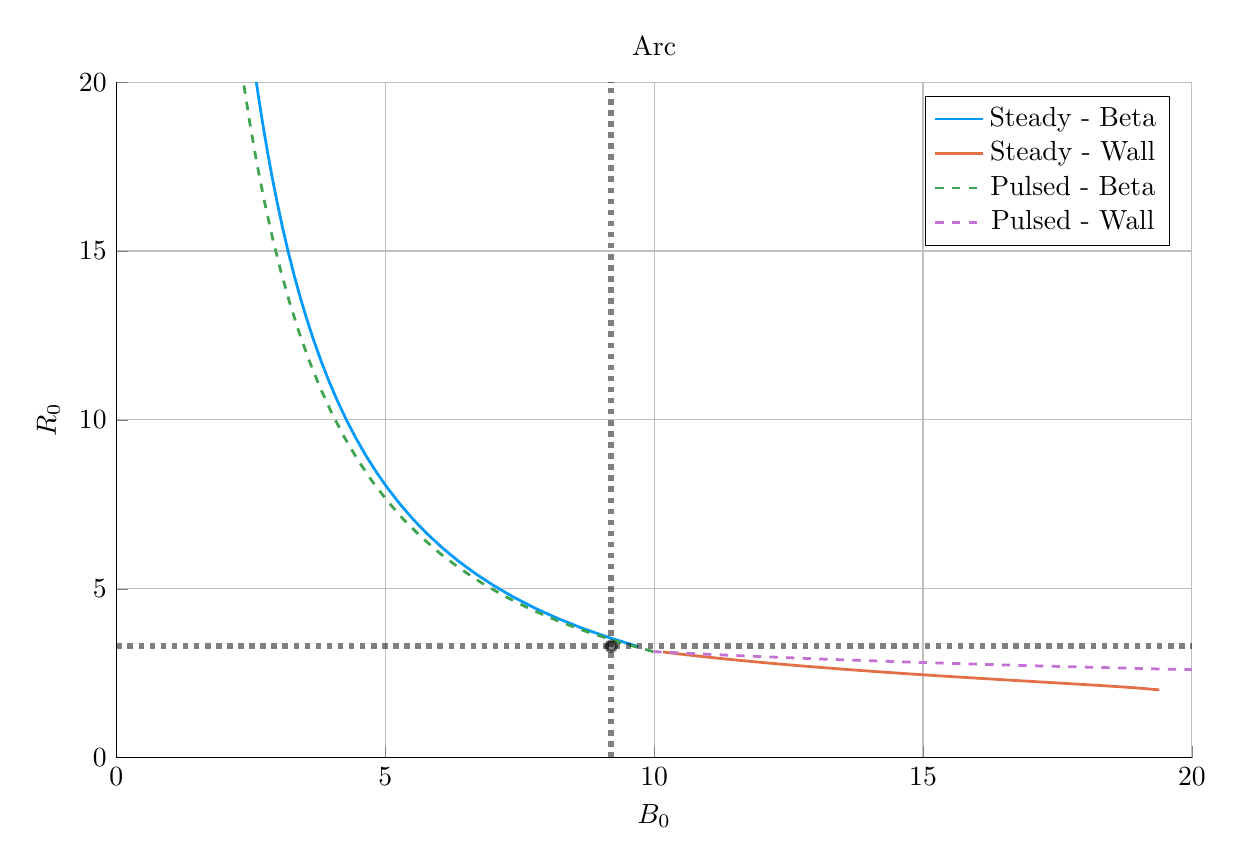
\begin{tikzpicture}[]
\begin{axis}[height = {101.6mm}, ylabel = {${R}_{0}$}, title = {Arc}, xmin = {0.0}, xmax = {20.0}, ymax = {20.0}, xlabel = {${B}_{0}$}, {unbounded coords=jump, scaled x ticks = false, xticklabel style={rotate = 0}, xmajorgrids = true, xtick = {0.0,5.0,10.0,15.0,20.0}, xticklabels = {0,5,10,15,20}, xtick align = inside, axis lines* = left, scaled y ticks = false, yticklabel style={rotate = 0}, ymajorgrids = true, ytick = {0.0,5.0,10.0,15.0,20.0}, yticklabels = {0,5,10,15,20}, ytick align = inside, axis lines* = left,     xshift = 0.0mm,
    yshift = 0.0mm,
    axis background/.style={fill={rgb,1:red,1.00000000;green,1.00000000;blue,1.00000000}}
, colorbar style={title=}}, ymin = {0.0}, width = {152.4mm}]\addplot+ [color = {rgb,1:red,0.00000000;green,0.60560316;blue,0.97868012},
draw opacity=1.0,
line width=1,
solid,mark = none,
mark size = 2.0,
mark options = {
    color = {rgb,1:red,0.00000000;green,0.00000000;blue,0.00000000}, draw opacity = 1.0,
    fill = {rgb,1:red,0.00000000;green,0.60560316;blue,0.97868012}, fill opacity = 1.0,
    line width = 1,
    rotate = 0,
    solid
}]coordinates {
(9.701206080853105, 3.2904233285656006)
(9.162315904693079, 3.553631706046861)
(8.664301107137337, 3.8315748016260343)
(8.203576462497304, 4.124583886864978)
(7.776718537485166, 4.433072975674755)
(7.380720231870917, 4.75741949036414)
(7.012886014999712, 5.097987291342331)
(6.670795005901889, 5.4551257000070565)
(6.352268997292712, 5.829168567645448)
(6.055344682097163, 6.220433393277178)
(5.778249464564785, 6.629220493040615)
(5.519380338856715, 7.05581222339423)
(5.2772854007125325, 7.500472260074458)
(5.050647625972996, 7.963444934423652)
(4.838270606140816, 8.444954628380609)
(4.639065978019038, 8.94520522910952)
(4.4520423235376105, 9.464379643936518)
(4.276295348572609, 10.002639375969222)
(4.110999177018484, 10.56012416048812)
(3.9553986195015125, 11.136951661929974)
(3.8088022956698633, 11.733217231026282)
(3.6705765055641186, 12.34899372141899)
(3.54013975965751, 12.984331364849716)
(3.4169578891619192, 13.639257703809928)
(3.30053966845824, 14.313777580345645)
(3.1904328903033052, 15.007873179535935)
(3.086220842019516, 15.721504126002731)
(2.9875191373772063, 16.45460763166718)
(2.8939728644914635, 17.207098692842226)
(2.8052540149097247, 17.97887033463821)
(2.7210591632720242, 18.7697939005645)
(2.6411073705789065, 19.579719385129263)
(2.565138287279709, 20.40847580717446)
(2.492910435164382, 21.255871621630877)
(2.4241996494611984, 22.12169516733927)
(2.3587976646588236, 23.0057151485579)
(2.296510829425685, 23.907681147764652)
(2.237158937627476, 24.827324167354146)
(2.180574163874242, 25.764357197843207)
(2.126600093288366, 26.71847581021091)
(2.075090836295778, 27.689358770027713)
(2.0259102202234582, 28.676668671060817)
(1.978931050353818, 29.68005258608471)
(1.9340344338545452, 30.69914273267572)
(1.8911091606836798, 31.733557151818793)
(1.8500511361739687, 32.78290039722107)
(1.8107628605384507, 33.846764233283025)
(1.773152951016952, 34.92472833975579)
(1.7371357028100902, 36.01636102117257)
(1.7026306853269466, 37.121219919229354)
(1.6695623706125668, 38.23885272635799)
(1.6378597911249178, 39.368797898817405)
(1.607456224302725, 40.51058536770822)
(1.5782889016090462, 41.663737246396295)
(1.5502987399539199, 42.82776853291479)
(1.5234300935954943, 44.00218780599217)
(1.4976305247952577, 45.18649791343829)
(1.4728505916614916, 46.38019665170201)
(1.4490436517578602, 47.58277743549339)
(1.4261656801829077, 48.79372995643627)
};
\addlegendentry{Steady - Beta}
\addplot+ [color = {rgb,1:red,0.88887350;green,0.43564919;blue,0.27812294},
draw opacity=1.0,
line width=1,
solid,mark = none,
mark size = 2.0,
mark options = {
    color = {rgb,1:red,0.00000000;green,0.00000000;blue,0.00000000}, draw opacity = 1.0,
    fill = {rgb,1:red,0.88887350;green,0.43564919;blue,0.27812294}, fill opacity = 1.0,
    line width = 1,
    rotate = 0,
    solid
}]coordinates {
(19.394007482712425, 2.006855814841082)
(18.932196567189358, 2.070220226465634)
(18.296989378345195, 2.1362327099649083)
(17.587029315408756, 2.2039322514902886)
(16.847882407994106, 2.272885741349308)
(16.111374502564406, 2.3427307443133163)
(15.396027314547156, 2.4132115621474344)
(14.710952688793137, 2.484165095168367)
(14.06168447794857, 2.555449485048069)
(13.450465418483889, 2.6269568263788754)
(12.877644538645335, 2.6986005527245354)
(12.342394470642008, 2.7703103261458715)
(11.843182246608265, 2.8420284550528074)
(11.376441269625893, 2.9137564749008216)
(10.944966372727551, 2.985307257194073)
(10.541663878705513, 3.056795384934831)
(10.165908182236457, 3.128148092221394)
};
\addlegendentry{Steady - Wall}
\addplot+ [color = {rgb,1:red,0.24222430;green,0.64327509;blue,0.30444865},
draw opacity=1.0,
line width=1,
dashed,mark = none,
mark size = 2.0,
mark options = {
    color = {rgb,1:red,0.00000000;green,0.00000000;blue,0.00000000}, draw opacity = 1.0,
    fill = {rgb,1:red,0.24222430;green,0.64327509;blue,0.30444865}, fill opacity = 1.0,
    line width = 1,
    rotate = 0,
    solid
}]coordinates {
(9.980483622051658, 3.1402982942956537)
(9.392786903460065, 3.3984668375583613)
(8.79273598103983, 3.7029994270206985)
(8.23820290909994, 4.029752381934837)
(7.725182218401588, 4.380005330007902)
(7.250078106370205, 4.755088191072525)
(6.80965553466646, 5.15638156809462)
(6.400998063035608, 5.585317075247801)
(6.0214713600430425, 6.043377623224966)
(5.668691517461799, 6.532097691007738)
(5.340497445229901, 7.053063624618788)
(5.034926745580058, 7.607914017422467)
(4.750194564008521, 8.198340243900201)
(4.484674995755211, 8.826087240213646)
(4.236884692979903, 9.49295465115087)
(4.00546837264544, 10.200798495308337)
(3.7891859704718387, 10.951533539957822)
(3.5869012239550364, 11.747136625739826)
(3.3975714987448393, 12.589651241396528)
(3.2202386987489797, 13.481193723261853)
(3.0540211220494466, 14.423961547290066)
(2.8981061427709687, 15.420244298711943)
(2.7517436139566023, 16.472438053930638)
(2.6142398986781377, 17.58306410230943)
(2.4849524463010138, 18.754793188384546)
(2.363284838174807, 19.990476791576892)
(2.248682232019848, 21.293187416028662)
(2.140627136740878, 22.666270490916787)
(2.038635448877246, 24.113411362836906)
(1.9422526775794744, 25.638722123308433)
(1.8510502754751532, 27.246854857488287)
(1.7646219756564088, 28.94315065234289)
(1.6825800061969869, 30.73383791051506)
(1.6045510059627948, 32.62630011975996)
(1.53017138625397, 34.629443897654504)
(1.4590817483192686, 36.754215952550474)
(1.3909197311384796, 39.01434852880224)
(1.3253102336217724, 41.42746903285954)
(1.261851128383913, 44.01681696754988)
(1.20009089049112, 46.81403058684408)
(1.1394908096975784, 49.863950342519615)
};
\addlegendentry{Pulsed - Beta}
\addplot+ [color = {rgb,1:red,0.76444018;green,0.44411178;blue,0.82429754},
draw opacity=1.0,
line width=1,
dashed,mark = none,
mark size = 2.0,
mark options = {
    color = {rgb,1:red,0.00000000;green,0.00000000;blue,0.00000000}, draw opacity = 1.0,
    fill = {rgb,1:red,0.76444018;green,0.44411178;blue,0.82429754}, fill opacity = 1.0,
    line width = 1,
    rotate = 0,
    solid
}]coordinates {
(29.27715761652869, 2.3448804182939873)
(25.4410619834368, 2.4377937236066716)
(22.158819835998365, 2.5322208586485804)
(19.342453256965573, 2.628163744265164)
(16.919364280634177, 2.7256238396687067)
(14.829378672669455, 2.8246020951898183)
(13.022412368922526, 2.9250989082568273)
(11.456617692058645, 3.0271140820266207)
(10.096901921254785, 3.1306467862637533)
(9.980483622051658, 3.1402982942956537)
};
\addlegendentry{Pulsed - Wall}
\addplot+ [color = {rgb,1:red,0.00000000;green,0.00000000;blue,0.00000000},
draw opacity=0.5,
line width=2,
dotted,mark = none,
mark size = 2.0,
mark options = {
    color = {rgb,1:red,0.00000000;green,0.00000000;blue,0.00000000}, draw opacity = 0.5,
    fill = {rgb,1:red,0.00000000;green,0.00000000;blue,0.00000000}, fill opacity = 0.5,
    line width = 1,
    rotate = 0,
    solid
},forget plot]coordinates {
(0.0, 3.3)
(20.0, 3.3)
};
\addplot+ [color = {rgb,1:red,0.00000000;green,0.00000000;blue,0.00000000},
draw opacity=0.5,
line width=2,
dotted,mark = none,
mark size = 2.0,
mark options = {
    color = {rgb,1:red,0.00000000;green,0.00000000;blue,0.00000000}, draw opacity = 0.5,
    fill = {rgb,1:red,0.00000000;green,0.00000000;blue,0.00000000}, fill opacity = 0.5,
    line width = 1,
    rotate = 0,
    solid
},forget plot]coordinates {
(9.2, 0.0)
(9.2, 20.0)
};
\addplot+[draw=none, color = {rgb,1:red,0.00000000;green,0.00000000;blue,0.00000000},
draw opacity=0.5,
line width=0,
solid,mark = *,
mark size = 2.0,
mark options = {
    color = {rgb,1:red,0.00000000;green,0.00000000;blue,0.00000000}, draw opacity = 0.5,
    fill = {rgb,1:red,0.00000000;green,0.00000000;blue,0.00000000}, fill opacity = 0.5,
    line width = 1,
    rotate = 0,
    solid
},forget plot] coordinates {
(9.2, 3.3)
};
\end{axis}

\end{tikzpicture}

    \end{adjustbox}
        \caption{$R_0$ vs $B_0$}
    \end{subfigure}
    \hfill
    \begin{subfigure}[t]{0.45\textwidth}
        \centering
    \begin{adjustbox}{width=\textwidth}
      \Large
      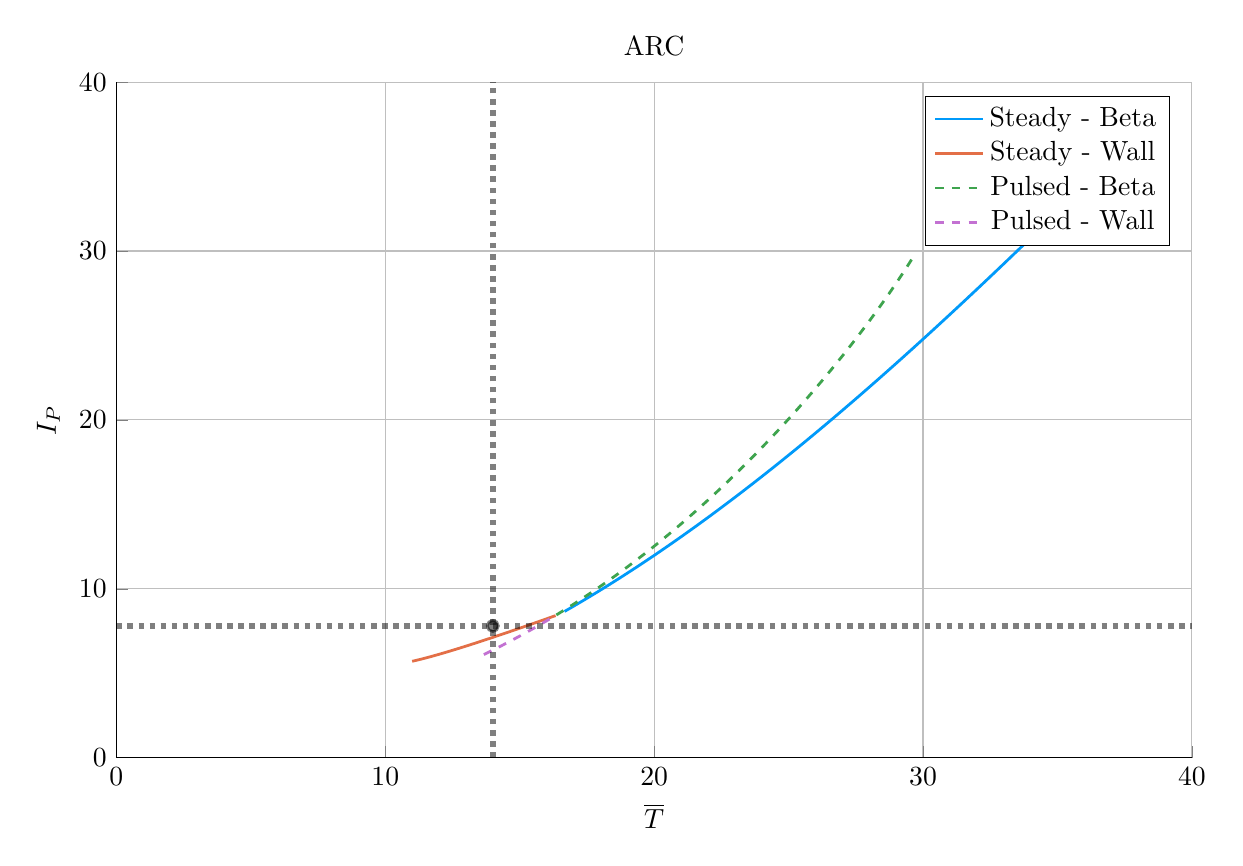
\begin{tikzpicture}[]
\begin{axis}[height = {101.6mm}, ylabel = {${I}_{P}$}, title = {ARC}, xmin = {0.0}, xmax = {40.0}, ymax = {40.0}, xlabel = {$\overline {T}$}, {unbounded coords=jump, scaled x ticks = false, xticklabel style={rotate = 0}, xmajorgrids = true, xtick = {0.0,10.0,20.0,30.0,40.0}, xticklabels = {0,10,20,30,40}, xtick align = inside, axis lines* = left, scaled y ticks = false, yticklabel style={rotate = 0}, ymajorgrids = true, ytick = {0.0,10.0,20.0,30.0,40.0}, yticklabels = {0,10,20,30,40}, ytick align = inside, axis lines* = left,     xshift = 0.0mm,
    yshift = 0.0mm,
    axis background/.style={fill={rgb,1:red,1.00000000;green,1.00000000;blue,1.00000000}}
, colorbar style={title=}}, ymin = {0.0}, width = {152.4mm}]\addplot+ [color = {rgb,1:red,0.00000000;green,0.60560316;blue,0.97868012},
draw opacity=1.0,
line width=1,
solid,mark = none,
mark size = 2.0,
mark options = {
    color = {rgb,1:red,0.00000000;green,0.00000000;blue,0.00000000}, draw opacity = 1.0,
    fill = {rgb,1:red,0.00000000;green,0.60560316;blue,0.97868012}, fill opacity = 1.0,
    line width = 1,
    rotate = 0,
    solid
}]coordinates {
(16.666666666666668, 8.658343870907427)
(17.0, 8.964855141636448)
(17.333333333333332, 9.277118721367206)
(17.666666666666668, 9.595036914426)
(18.0, 9.918585776352757)
(18.333333333333332, 10.247718935951552)
(18.666666666666668, 10.582387319200262)
(19.0, 10.922539274323045)
(19.333333333333332, 11.26812069483817)
(19.666666666666668, 11.61907514056121)
(20.0, 11.975343956529299)
(20.333333333333332, 12.336866389803589)
(20.666666666666668, 12.703579704100664)
(21.0, 13.07541929220057)
(21.333333333333332, 13.452318786079019)
(21.666666666666668, 13.834210164711733)
(22.0, 14.221023859501257)
(22.333333333333332, 14.61268885728139)
(22.666666666666668, 15.009132800857182)
(23.0, 15.410282087044596)
(23.333333333333332, 15.816061962178953)
(23.666666666666668, 16.226396615066992)
(24.0, 16.64120926736311)
(24.333333333333332, 17.060422261356294)
(24.666666666666668, 17.483957145159597)
(25.0, 17.91173475530017)
(25.333333333333332, 18.343675296712746)
(25.666666666666668, 18.77969842014449)
(26.0, 19.2197232969848)
(26.333333333333332, 19.663668691537165)
(26.666666666666668, 20.11145303075519)
(27.0, 20.562994471468567)
(27.333333333333332, 21.018210965128485)
(27.666666666666668, 21.477020320105293)
(28.0, 21.939340261574117)
(28.333333333333332, 22.405088489026962)
(28.666666666666668, 22.874182731452617)
(29.0, 23.34654080022686)
(29.333333333333332, 23.82208063975841)
(29.666666666666668, 24.300720375936947)
(30.0, 24.782378362431352)
(30.333333333333332, 25.26697322488704)
(30.666666666666668, 25.754423903072542)
(31.0, 26.244649691026318)
(31.333333333333332, 26.737570275254438)
(31.666666666666668, 27.233105771031717)
(32.0, 27.731176756857092)
(32.333333333333336, 28.23170430711659)
(32.666666666666664, 28.734610023004112)
(33.0, 29.23981606175298)
(33.333333333333336, 29.747245164229085)
(33.666666666666664, 30.256820680936514)
(34.0, 30.768466596486252)
(34.333333333333336, 31.282107552577845)
(34.666666666666664, 31.797668869543177)
(35.0, 32.31507656650066)
(35.333333333333336, 32.83425738016771)
(35.666666666666664, 33.35513878237846)
(36.0, 33.87764899635294)
(36.333333333333336, 34.40171701176134)
};
\addlegendentry{Steady - Beta}
\addplot+ [color = {rgb,1:red,0.88887350;green,0.43564919;blue,0.27812294},
draw opacity=1.0,
line width=1,
solid,mark = none,
mark size = 2.0,
mark options = {
    color = {rgb,1:red,0.00000000;green,0.00000000;blue,0.00000000}, draw opacity = 1.0,
    fill = {rgb,1:red,0.88887350;green,0.43564919;blue,0.27812294}, fill opacity = 1.0,
    line width = 1,
    rotate = 0,
    solid
}]coordinates {
(11.0, 5.705363947896813)
(11.333333333333334, 5.831631927327359)
(11.666666666666666, 5.971358416795512)
(12.0, 6.120248050030096)
(12.333333333333334, 6.27635241161913)
(12.666666666666666, 6.438084943966173)
(13.0, 6.6043437111573775)
(13.333333333333334, 6.774432932493379)
(13.666666666666666, 6.9477586358526295)
(14.0, 7.123875039246037)
(14.333333333333334, 7.302428845502918)
(14.666666666666666, 7.483135839919747)
(15.0, 7.66576464137543)
(15.333333333333334, 7.850323804140159)
(15.666666666666666, 8.036059275223955)
(16.0, 8.223435700494395)
(16.333333333333332, 8.412159667095638)
};
\addlegendentry{Steady - Wall}
\addplot+ [color = {rgb,1:red,0.24222430;green,0.64327509;blue,0.30444865},
draw opacity=1.0,
line width=1,
dashed,mark = none,
mark size = 2.0,
mark options = {
    color = {rgb,1:red,0.00000000;green,0.00000000;blue,0.00000000}, draw opacity = 1.0,
    fill = {rgb,1:red,0.24222430;green,0.64327509;blue,0.30444865}, fill opacity = 1.0,
    line width = 1,
    rotate = 0,
    solid
}]coordinates {
(16.364160609330686, 8.45211123232532)
(16.666666666666668, 8.749174237506722)
(17.0, 9.084875445329175)
(17.333333333333332, 9.429466194729264)
(17.666666666666668, 9.783065958753857)
(18.0, 10.145791398086809)
(18.333333333333332, 10.517756265001724)
(18.666666666666668, 10.899071333792335)
(19.0, 11.28984436597908)
(19.333333333333332, 11.690180120182706)
(19.666666666666668, 12.100180418434789)
(20.0, 12.519944282916168)
(20.333333333333332, 12.949568159742276)
(20.666666666666668, 13.389146249526421)
(21.0, 13.838770968145022)
(21.333333333333332, 14.298533565526986)
(21.666666666666668, 14.768524935556082)
(22.0, 15.2488366565296)
(22.333333333333332, 15.739562309352701)
(22.666666666666668, 16.240799130174846)
(23.0, 16.752650066058415)
(23.333333333333332, 17.27522631730515)
(23.666666666666668, 17.808650469386293)
(24.0, 18.353060342640163)
(24.333333333333332, 18.908613721362002)
(24.666666666666668, 19.475494169025602)
(25.0, 20.053918198206937)
(25.333333333333332, 20.644144149900036)
(25.666666666666668, 21.246483258877372)
(26.0, 21.861313557471373)
(26.333333333333332, 22.48909752802998)
(26.666666666666668, 23.130404800381292)
(27.0, 23.785941781633092)
(27.333333333333332, 24.456591033172632)
(27.666666666666668, 25.143464707502787)
(28.0, 25.84797885666414)
(28.333333333333332, 26.571959755666764)
(28.666666666666668, 27.3178012356156)
(29.0, 28.088707029156687)
(29.333333333333332, 28.889082725820668)
(29.666666666666668, 29.725209471035893)
};
\addlegendentry{Pulsed - Beta}
\addplot+ [color = {rgb,1:red,0.76444018;green,0.44411178;blue,0.82429754},
draw opacity=1.0,
line width=1,
dashed,mark = none,
mark size = 2.0,
mark options = {
    color = {rgb,1:red,0.00000000;green,0.00000000;blue,0.00000000}, draw opacity = 1.0,
    fill = {rgb,1:red,0.76444018;green,0.44411178;blue,0.82429754}, fill opacity = 1.0,
    line width = 1,
    rotate = 0,
    solid
}]coordinates {
(13.666666666666666, 6.106956435644008)
(14.0, 6.368429153074452)
(14.333333333333334, 6.637611037727747)
(14.666666666666666, 6.914640849606676)
(15.0, 7.199655680909235)
(15.333333333333334, 7.492790823032018)
(15.666666666666666, 7.794179619860046)
(16.0, 8.103953307930404)
(16.333333333333332, 8.422240844292133)
(16.364160609330686, 8.45211123232532)
};
\addlegendentry{Pulsed - Wall}
\addplot+ [color = {rgb,1:red,0.00000000;green,0.00000000;blue,0.00000000},
draw opacity=0.5,
line width=2,
dotted,mark = none,
mark size = 2.0,
mark options = {
    color = {rgb,1:red,0.00000000;green,0.00000000;blue,0.00000000}, draw opacity = 0.5,
    fill = {rgb,1:red,0.00000000;green,0.00000000;blue,0.00000000}, fill opacity = 0.5,
    line width = 1,
    rotate = 0,
    solid
},forget plot]coordinates {
(0.0, 7.8)
(40.0, 7.8)
};
\addplot+ [color = {rgb,1:red,0.00000000;green,0.00000000;blue,0.00000000},
draw opacity=0.5,
line width=2,
dotted,mark = none,
mark size = 2.0,
mark options = {
    color = {rgb,1:red,0.00000000;green,0.00000000;blue,0.00000000}, draw opacity = 0.5,
    fill = {rgb,1:red,0.00000000;green,0.00000000;blue,0.00000000}, fill opacity = 0.5,
    line width = 1,
    rotate = 0,
    solid
},forget plot]coordinates {
(14.0, 0.0)
(14.0, 40.0)
};
\addplot+[draw=none, color = {rgb,1:red,0.00000000;green,0.00000000;blue,0.00000000},
draw opacity=0.5,
line width=0,
solid,mark = *,
mark size = 2.0,
mark options = {
    color = {rgb,1:red,0.00000000;green,0.00000000;blue,0.00000000}, draw opacity = 0.5,
    fill = {rgb,1:red,0.00000000;green,0.00000000;blue,0.00000000}, fill opacity = 0.5,
    line width = 1,
    rotate = 0,
    solid
},forget plot] coordinates {
(14.0, 7.8)
};
\end{axis}

\end{tikzpicture}

    \end{adjustbox}
        \caption{$I_P$ vs $\overline T$}
    \end{subfigure}
    \hfill \hfill ~\\ ~\\ ~\\
    \caption{Arc Model Comparison} ~\\
\end{figure*}

\begin{table}[h!]
\centering  
\caption{Arc Variables}
\hfill
\begin{subtable}[t]{0.4\textwidth}
\centering  
\caption{Input Variables} ~\\
\begin{tabular}{ c|c } 

Input            & Value           \\
\hline
$H$              & 1.8             \\
$Q$              & 13.6            \\
$N_{G}$          & 0.67            \\
$\epsilon$       & 0.333          \\
$\kappa_{95}$    & 1.84            \\
$\delta_{95}$    & 0.333           \\
$\nu_{n}$        & 0.385           \\
$\nu_{T}$        & 0.929           \\
$l_{i}$          & 0.67            \\
$A$              & 2.5             \\
$Z_{eff}$        & 1.2             \\
$f_{D}$          & 0.9             \\
$\tau_{FT}$      & 1.6e9           \\
$B_{CS}$         & 12.77           \\

\end{tabular}
\end{subtable}
\hfill
\begin{subtable}[t]{0.5\textwidth}
\centering  
\caption{Output Variables} ~\\
\begin{tabular}{ c|c|c } 

Output           & Original         & Fussy.jl        \\
\hline
$R_{0}$          & 3.3              & 3.4           \\
$B_{0}$          & 9.2              & 9.5           \\
$I_{P}$          & 7.8              & 8.8           \\
$\overline n$    & 1.3              & 1.3           \\
$\overline T$    & 14.0             & 16.8           \\
$\beta_{N}$       & 0.026           & -          \\
$q_{95}$         & 7.2              & 6.1           \\
$P_{W}$          & 2.5              & 2.2           \\
$f_{BS}$         & 0.63             & 0.56          \\
$f_{CD}$         & 0.37             & 0.44          \\
$f_{ID}$         & -              & -             \\
$\volume$         & 141            & 157           \\
$P_{F}$          & 525            & 726           \\
$\eta_{CD}$      & 0.321            & 0.316          \\

\end{tabular}
\end{subtable}
\hfill
\hfill
\end{table}

\newpage

\subsection{Contrasting with the Aries Act Studies}

Moving on, the Aries Act study focuses on how steady-state reactors would look under both a conservative and optimistic perspective. This is highlighted in \cref{fig:act_h_cost}, which shows how costs decreases as the H factor is allowed to increase. Notice that for every value of H, the ACT I study (i.e. the optimistic act) has a lower cost than the design from ACT II (i.e. the conservative one).

This figure also highlights another peculiarity of the ARIES study -- a reliance on the minimum possible value of H. Note that just left of the reactor point on both plots is a highly erratic portion of the curve. As such, if even a slightly smaller value of H were used in either case, a quite distinct reactor would occur. This is not a robust way to design machines. A better approach would be to build with some safety factor -- i.e at a slightly more magical version of H. This can be seen in ARC's H-Sweep.

\begin{figure*}[h!]
    \centering
    \hfill 
    \begin{subfigure}[t]{0.4\textwidth}
        \centering
    \begin{adjustbox}{width=\textwidth}
      \Large
      \begin{tikzpicture}[]
\begin{axis}[height = {101.6mm}, ylabel = {${C}_{W}$}, title = {Act I}, xmin = {0.0}, xmax = {3.9599999999999995}, ymax = {0.1}, xlabel = {${H}$}, {unbounded coords=jump, scaled x ticks = false, xticklabel style={rotate = 0}, xmajorgrids = true, xtick = {0.0,1.0,2.0,3.0}, xticklabels = {0,1,2,3}, xtick align = inside, axis lines* = left, scaled y ticks = false, yticklabel style={rotate = 0}, ymajorgrids = true, ytick = {0.0,0.02,0.04,0.06,0.08,0.1}, yticklabels = {0.00,0.02,0.04,0.06,0.08,0.10}, ytick align = inside, axis lines* = left,     xshift = 0.0mm,
    yshift = 0.0mm,
    axis background/.style={fill={rgb,1:red,1.00000000;green,1.00000000;blue,1.00000000}}
, colorbar style={title=}}, ymin = {0.0}, width = {152.4mm}]\addplot+ [color = {rgb,1:red,0.88887350;green,0.43564919;blue,0.27812294},
draw opacity=0.7,
line width=3,
dotted,mark = none,
mark size = 2.0,
mark options = {
    color = {rgb,1:red,0.00000000;green,0.00000000;blue,0.00000000}, draw opacity = 0.7,
    fill = {rgb,1:red,0.88887350;green,0.43564919;blue,0.27812294}, fill opacity = 0.7,
    line width = 1,
    rotate = 0,
    solid
}]coordinates {
(1.65, 0.0038580882449725513)
(1.7325, 0.0034224421580344765)
(1.815, 0.0031242773601625963)
(1.8975, 0.0029076912463966475)
(1.98, 0.0027437459144664237)
(2.0625, 0.002615755758688704)
(2.145, 0.0025133725117807595)
};
\addlegendentry{$wall$}
\addplot+ [color = {rgb,1:red,0.24222430;green,0.64327509;blue,0.30444865},
draw opacity=0.7,
line width=1,
solid,mark = none,
mark size = 2.0,
mark options = {
    color = {rgb,1:red,0.00000000;green,0.00000000;blue,0.00000000}, draw opacity = 0.7,
    fill = {rgb,1:red,0.24222430;green,0.64327509;blue,0.30444865}, fill opacity = 0.7,
    line width = 1,
    rotate = 0,
    solid
}]coordinates {
(1.4025, 0.025918216479107938)
(1.485, 0.012095504772150555)
(1.5675, 0.005882239716429097)
(1.65, 0.0038447827755938714)
(1.7325, 0.0034077229105716356)
(1.815, 0.0031112188891089447)
(1.8975, 0.002896491612881698)
(1.98, 0.002734083771296579)
(2.0625, 0.002607278997942983)
(2.145, 0.002505795370579703)
(2.2275, 0.0024978293322600134)
(2.31, 0.0026050612316072053)
(2.3925, 0.002711328730788369)
(2.475, 0.0028163739703009525)
(2.5575, 0.002920119984789825)
(2.64, 0.0030223238461750735)
(2.7225, 0.003122910039550508)
(2.805, 0.003221795626029453)
(2.8875, 0.003318919864510233)
(2.97, 0.003414240640857473)
(3.0525, 0.003507731326910594)
(3.135, 0.003599378182186399)
(3.2175, 0.00368917819814934)
(3.3, 0.003777137172338829)
};
\addlegendentry{$cost$}
\addplot+ [color = {rgb,1:red,0.76444018;green,0.44411178;blue,0.82429754},
draw opacity=0.7,
line width=1,
solid,mark = none,
mark size = 2.0,
mark options = {
    color = {rgb,1:red,0.00000000;green,0.00000000;blue,0.00000000}, draw opacity = 0.7,
    fill = {rgb,1:red,0.76444018;green,0.44411178;blue,0.82429754}, fill opacity = 0.7,
    line width = 1,
    rotate = 0,
    solid
}]coordinates {
(1.4025, 0.02636776101728183)
(1.485, 0.018483166138998787)
(1.5675, 0.007170526433976295)
(1.65, 0.003841721357482374)
(1.7325, 0.0034053745614292777)
(1.815, 0.0031097242744622163)
(1.8975, 0.002895546190157591)
(1.98, 0.0027334738346990873)
(2.0625, 0.002606876408558846)
(2.145, 0.0025055240752749086)
(2.2275, 0.0024978197141057924)
(2.31, 0.0026050530799257014)
(2.3925, 0.0027113218095688846)
(2.475, 0.0028164020534254693)
(2.5575, 0.0029201149972198264)
(2.64, 0.0030223196276555316)
(2.7225, 0.003122906476745389)
(2.805, 0.0032217926032687013)
(2.8875, 0.0033189173512138603)
(2.97, 0.0034142385345432096)
(3.0525, 0.0035077295453675586)
(3.135, 0.0035993767225118564)
(3.2175, 0.003689176968945425)
(3.3, 0.0037771361544507143)
};
\addlegendentry{$W_M$}
\addplot+ [color = {rgb,1:red,0.67554396;green,0.55566233;blue,0.09423434},
draw opacity=1.0,
line width=1,
dashed,mark = none,
mark size = 2.0,
mark options = {
    color = {rgb,1:red,0.00000000;green,0.00000000;blue,0.00000000}, draw opacity = 1.0,
    fill = {rgb,1:red,0.67554396;green,0.55566233;blue,0.09423434}, fill opacity = 1.0,
    line width = 1,
    rotate = 0,
    solid
},forget plot]coordinates {
(1.65, 0.0)
(1.65, 0.1)
};
\addplot+ [color = {rgb,1:red,0.00000048;green,0.66575898;blue,0.68099695},
draw opacity=1.0,
line width=1,
dashed,mark = none,
mark size = 2.0,
mark options = {
    color = {rgb,1:red,0.00000000;green,0.00000000;blue,0.00000000}, draw opacity = 1.0,
    fill = {rgb,1:red,0.00000048;green,0.66575898;blue,0.68099695}, fill opacity = 1.0,
    line width = 1,
    rotate = 0,
    solid
},forget plot]coordinates {
(0.0, 0.0)
(0.0, 0.1)
};
\addplot+ [color = {rgb,1:red,0.00000048;green,0.66575898;blue,0.68099695},
draw opacity=1.0,
line width=1,
dashed,mark = none,
mark size = 2.0,
mark options = {
    color = {rgb,1:red,0.00000000;green,0.00000000;blue,0.00000000}, draw opacity = 1.0,
    fill = {rgb,1:red,0.00000048;green,0.66575898;blue,0.68099695}, fill opacity = 1.0,
    line width = 1,
    rotate = 0,
    solid
},forget plot]coordinates {
(3.3, 0.0)
(3.3, 0.1)
};
\end{axis}

\end{tikzpicture}

    \end{adjustbox}
        \caption{Act I H Sweep}
    \end{subfigure}
    \hfill
    \begin{subfigure}[t]{0.4\textwidth}
        \centering
    \begin{adjustbox}{width=\textwidth}
      \Large
      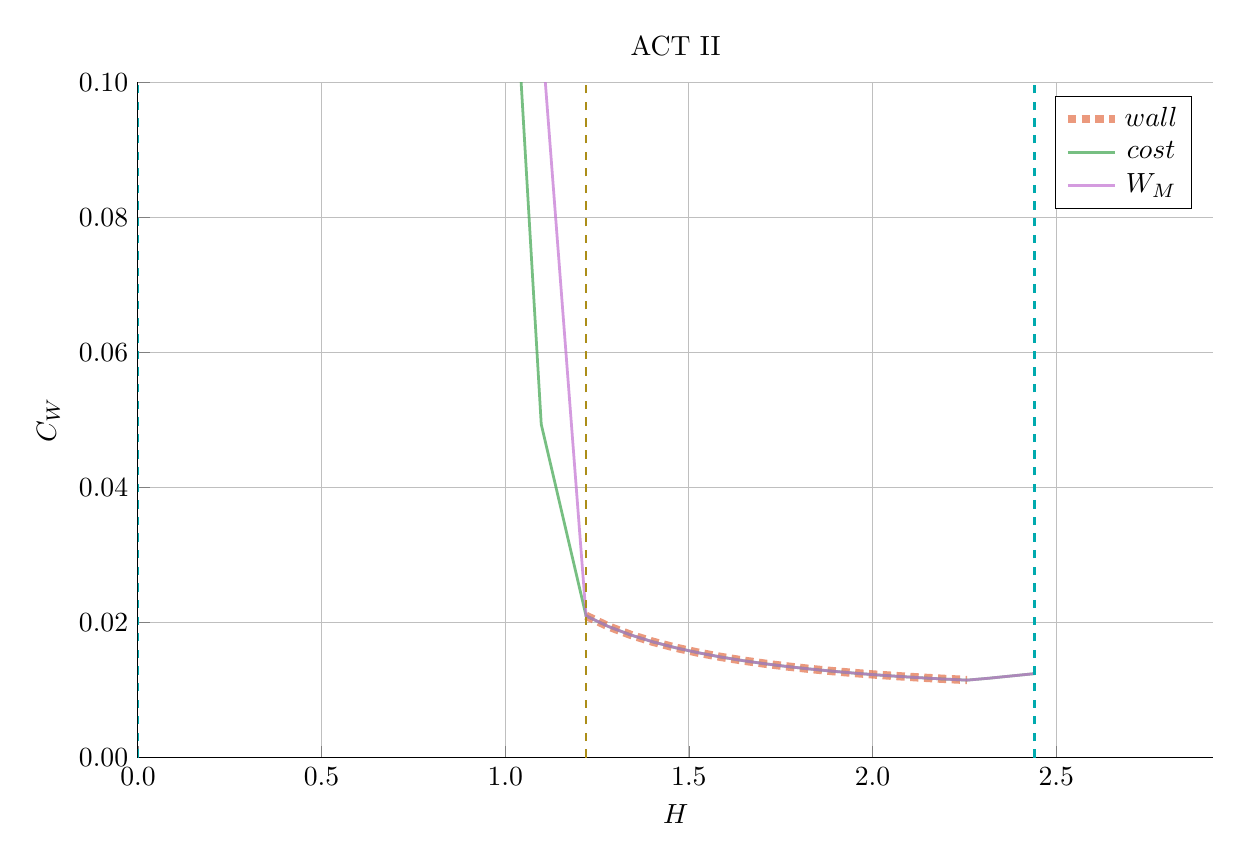
\begin{tikzpicture}[]
\begin{axis}[height = {101.6mm}, ylabel = {${C}_{W}$}, title = {ACT II}, xmin = {0.0}, xmax = {2.928}, ymax = {0.1}, xlabel = {${H}$}, {unbounded coords=jump, scaled x ticks = false, xticklabel style={rotate = 0}, xmajorgrids = true, xtick = {0.0,0.5,1.0,1.5,2.0,2.5}, xticklabels = {0.0,0.5,1.0,1.5,2.0,2.5}, xtick align = inside, axis lines* = left, scaled y ticks = false, yticklabel style={rotate = 0}, ymajorgrids = true, ytick = {0.0,0.02,0.04,0.06,0.08,0.1}, yticklabels = {0.00,0.02,0.04,0.06,0.08,0.10}, ytick align = inside, axis lines* = left,     xshift = 0.0mm,
    yshift = 0.0mm,
    axis background/.style={fill={rgb,1:red,1.00000000;green,1.00000000;blue,1.00000000}}
, colorbar style={title=}}, ymin = {0.0}, width = {152.4mm}]\addplot+ [color = {rgb,1:red,0.88887350;green,0.43564919;blue,0.27812294},
draw opacity=0.7,
line width=3,
dotted,mark = none,
mark size = 2.0,
mark options = {
    color = {rgb,1:red,0.00000000;green,0.00000000;blue,0.00000000}, draw opacity = 0.7,
    fill = {rgb,1:red,0.88887350;green,0.43564919;blue,0.27812294}, fill opacity = 0.7,
    line width = 1,
    rotate = 0,
    solid
}]coordinates {
(1.22, 0.021005512518330174)
(1.281, 0.01942744270360855)
(1.342, 0.018170389811630824)
(1.403, 0.017139710886836464)
(1.464, 0.01627794436788193)
(1.525, 0.015546450836866612)
(1.586, 0.014919600022944367)
(1.647, 0.014377436937475022)
(1.708, 0.013905581766222853)
(1.769, 0.01349265356023887)
(1.83, 0.013129558656358339)
(1.891, 0.01280891244140467)
(1.952, 0.012524569645508304)
(2.013, 0.01227184717788876)
(2.074, 0.012046102834086084)
(2.135, 0.01184360516877147)
(2.196, 0.011661349792575638)
(2.257, 0.011496773538316084)
};
\addlegendentry{$wall$}
\addplot+ [color = {rgb,1:red,0.24222430;green,0.64327509;blue,0.30444865},
draw opacity=0.7,
line width=1,
solid,mark = none,
mark size = 2.0,
mark options = {
    color = {rgb,1:red,0.00000000;green,0.00000000;blue,0.00000000}, draw opacity = 0.7,
    fill = {rgb,1:red,0.24222430;green,0.64327509;blue,0.30444865}, fill opacity = 0.7,
    line width = 1,
    rotate = 0,
    solid
}]coordinates {
(1.037, 0.10576482650233505)
(1.098, 0.04935829436307264)
(1.22, 0.020990970199014802)
(1.281, 0.0194129595370893)
(1.342, 0.01815662533322952)
(1.403, 0.01712672739309554)
(1.464, 0.016265578765863785)
(1.525, 0.015534719386234706)
(1.586, 0.014908297877268767)
(1.647, 0.014366575271189693)
(1.708, 0.013895114510245749)
(1.769, 0.013482541510434981)
(1.83, 0.013119766959557726)
(1.891, 0.012796621459369077)
(1.952, 0.012503284271399288)
(2.013, 0.012246990247871287)
(2.074, 0.012019443303647051)
(2.135, 0.011815835760118812)
(2.196, 0.011632962604193957)
(2.257, 0.011474758216077388)
(2.318, 0.011765579200211946)
(2.379, 0.012101340215422274)
(2.44, 0.012432978177363389)
};
\addlegendentry{$cost$}
\addplot+ [color = {rgb,1:red,0.76444018;green,0.44411178;blue,0.82429754},
draw opacity=0.7,
line width=1,
solid,mark = none,
mark size = 2.0,
mark options = {
    color = {rgb,1:red,0.00000000;green,0.00000000;blue,0.00000000}, draw opacity = 0.7,
    fill = {rgb,1:red,0.76444018;green,0.44411178;blue,0.82429754}, fill opacity = 0.7,
    line width = 1,
    rotate = 0,
    solid
}]coordinates {
(1.098, 0.10789687618345375)
(1.22, 0.020993563020398034)
(1.281, 0.019414381524971283)
(1.342, 0.018157569810455732)
(1.403, 0.017127496371177657)
(1.464, 0.016266077641847662)
(1.525, 0.015535219465132215)
(1.586, 0.014908546212398566)
(1.647, 0.014366740003006752)
(1.708, 0.013895218421357018)
(1.769, 0.01348260263682947)
(1.83, 0.013119799308255348)
(1.891, 0.0127993859843838)
(1.952, 0.012506614611284711)
(2.013, 0.01224686415179682)
(2.074, 0.012019222925033022)
(2.135, 0.011815568425293648)
(2.196, 0.011632678053496345)
(2.257, 0.011474127813480542)
(2.318, 0.011765572318494604)
(2.379, 0.012101333413489)
(2.44, 0.012432971811628111)
};
\addlegendentry{$W_M$}
\addplot+ [color = {rgb,1:red,0.67554396;green,0.55566233;blue,0.09423434},
draw opacity=1.0,
line width=1,
dashed,mark = none,
mark size = 2.0,
mark options = {
    color = {rgb,1:red,0.00000000;green,0.00000000;blue,0.00000000}, draw opacity = 1.0,
    fill = {rgb,1:red,0.67554396;green,0.55566233;blue,0.09423434}, fill opacity = 1.0,
    line width = 1,
    rotate = 0,
    solid
},forget plot]coordinates {
(1.22, 0.0)
(1.22, 0.1)
};
\addplot+ [color = {rgb,1:red,0.00000048;green,0.66575898;blue,0.68099695},
draw opacity=1.0,
line width=1,
dashed,mark = none,
mark size = 2.0,
mark options = {
    color = {rgb,1:red,0.00000000;green,0.00000000;blue,0.00000000}, draw opacity = 1.0,
    fill = {rgb,1:red,0.00000048;green,0.66575898;blue,0.68099695}, fill opacity = 1.0,
    line width = 1,
    rotate = 0,
    solid
},forget plot]coordinates {
(0.0, 0.0)
(0.0, 0.1)
};
\addplot+ [color = {rgb,1:red,0.00000048;green,0.66575898;blue,0.68099695},
draw opacity=1.0,
line width=1,
dashed,mark = none,
mark size = 2.0,
mark options = {
    color = {rgb,1:red,0.00000000;green,0.00000000;blue,0.00000000}, draw opacity = 1.0,
    fill = {rgb,1:red,0.00000048;green,0.66575898;blue,0.68099695}, fill opacity = 1.0,
    line width = 1,
    rotate = 0,
    solid
},forget plot]coordinates {
(2.44, 0.0)
(2.44, 0.1)
};
\end{axis}

\end{tikzpicture}

    \end{adjustbox}
        \caption{Act II H Sweep}
    \end{subfigure}
    \hfill \hfill ~\\ ~\\ ~\\
    \begin{subfigure}[t]{0.4\textwidth}
        \centering
		\begin{adjustbox}{width=\textwidth}
			\Large
			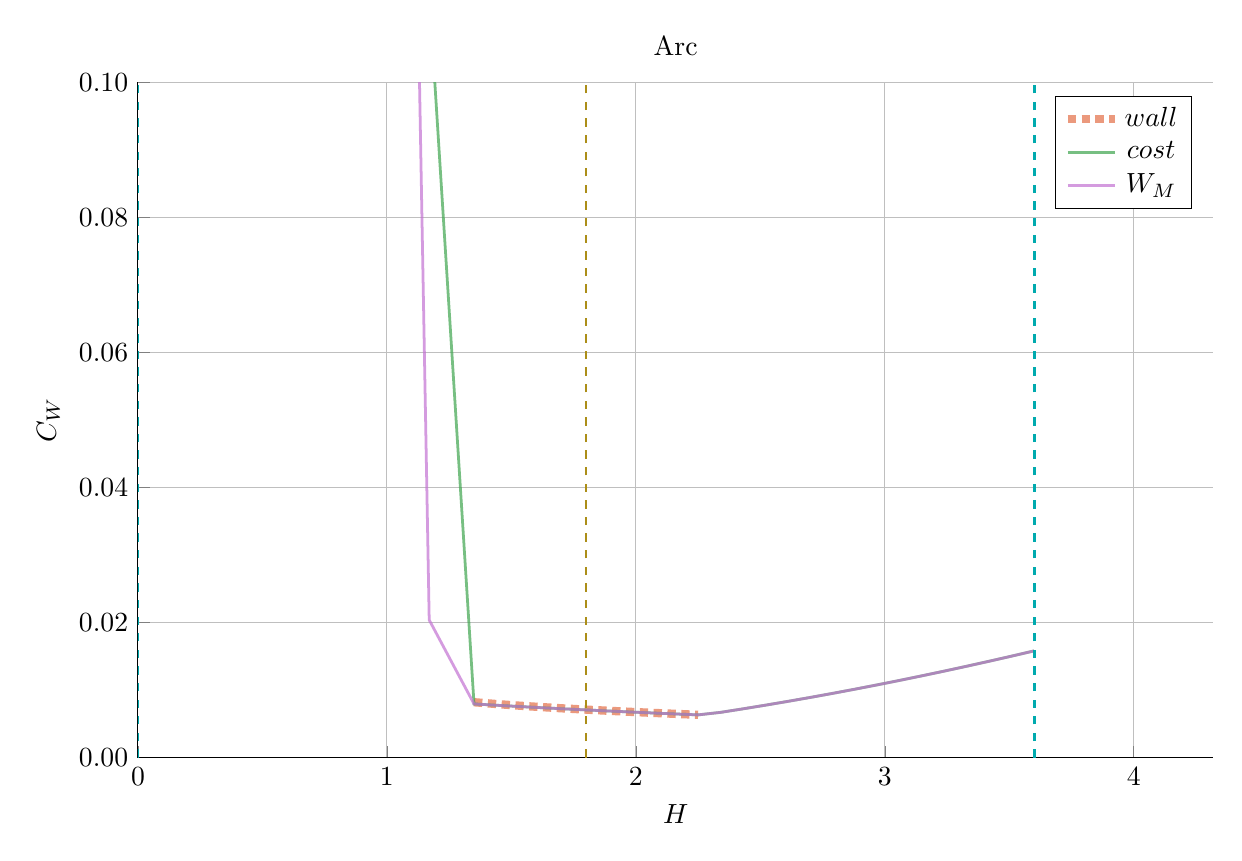
\begin{tikzpicture}[]
\begin{axis}[height = {101.6mm}, ylabel = {${C}_{W}$}, title = {Arc}, xmin = {0.0}, xmax = {4.32}, ymax = {0.1}, xlabel = {${H}$}, {unbounded coords=jump, scaled x ticks = false, xticklabel style={rotate = 0}, xmajorgrids = true, xtick = {0.0,1.0,2.0,3.0,4.0}, xticklabels = {0,1,2,3,4}, xtick align = inside, axis lines* = left, scaled y ticks = false, yticklabel style={rotate = 0}, ymajorgrids = true, ytick = {0.0,0.02,0.04,0.06,0.08,0.1}, yticklabels = {0.00,0.02,0.04,0.06,0.08,0.10}, ytick align = inside, axis lines* = left,     xshift = 0.0mm,
    yshift = 0.0mm,
    axis background/.style={fill={rgb,1:red,1.00000000;green,1.00000000;blue,1.00000000}}
, colorbar style={title=}}, ymin = {0.0}, width = {152.4mm}]\addplot+ [color = {rgb,1:red,0.88887350;green,0.43564919;blue,0.27812294},
draw opacity=0.7,
line width=3,
dotted,mark = none,
mark size = 2.0,
mark options = {
    color = {rgb,1:red,0.00000000;green,0.00000000;blue,0.00000000}, draw opacity = 0.7,
    fill = {rgb,1:red,0.88887350;green,0.43564919;blue,0.27812294}, fill opacity = 0.7,
    line width = 1,
    rotate = 0,
    solid
}]coordinates {
(1.35, 0.008207241762396246)
(1.44, 0.00793667759257354)
(1.53, 0.0076997912429461225)
(1.62, 0.007486816554981894)
(1.71, 0.007291648689881567)
(1.8, 0.007110333347796811)
(1.89, 0.006940248814588952)
(1.98, 0.006779633349026309)
(2.07, 0.006627297197584387)
(2.16, 0.006482438866566955)
(2.25, 0.006344768968841929)
};
\addlegendentry{$wall$}
\addplot+ [color = {rgb,1:red,0.24222430;green,0.64327509;blue,0.30444865},
draw opacity=0.7,
line width=1,
solid,mark = none,
mark size = 2.0,
mark options = {
    color = {rgb,1:red,0.00000000;green,0.00000000;blue,0.00000000}, draw opacity = 0.7,
    fill = {rgb,1:red,0.24222430;green,0.64327509;blue,0.30444865}, fill opacity = 0.7,
    line width = 1,
    rotate = 0,
    solid
}]coordinates {
(1.08, 0.1656933786109522)
(1.35, 0.007956028922350611)
(1.44, 0.007759662745290108)
(1.53, 0.007574913322065527)
(1.62, 0.00739885086770846)
(1.71, 0.0072297906534508185)
(1.8, 0.007066784363464752)
(1.89, 0.00690932755478892)
(1.98, 0.006757201835765392)
(2.07, 0.006610359300650354)
(2.16, 0.0064688545800951625)
(2.25, 0.006332913629979953)
(2.34, 0.00670268792962123)
(2.43, 0.0072243580642261445)
(2.52, 0.007766406785339575)
(2.61, 0.008328785580854575)
(2.7, 0.008911412315791628)
(2.79, 0.00951417119398493)
(2.88, 0.010136912409268534)
(2.97, 0.010779452862615483)
(3.06, 0.011441576670944502)
(3.15, 0.012123036438828786)
(3.24, 0.012823554577929932)
(3.33, 0.0135428254017145)
(3.42, 0.014280516598644705)
(3.51, 0.015036271676563144)
(3.6, 0.01580971210009804)
};
\addlegendentry{$cost$}
\addplot+ [color = {rgb,1:red,0.76444018;green,0.44411178;blue,0.82429754},
draw opacity=0.7,
line width=1,
solid,mark = none,
mark size = 2.0,
mark options = {
    color = {rgb,1:red,0.00000000;green,0.00000000;blue,0.00000000}, draw opacity = 0.7,
    fill = {rgb,1:red,0.76444018;green,0.44411178;blue,0.82429754}, fill opacity = 0.7,
    line width = 1,
    rotate = 0,
    solid
}]coordinates {
(1.08, 0.20419403931121408)
(1.17, 0.02038194154635263)
(1.35, 0.007952462446561684)
(1.44, 0.007756882763096937)
(1.53, 0.007572765485693452)
(1.62, 0.007397214242173672)
(1.71, 0.007228584574974498)
(1.8, 0.007065962995902896)
(1.89, 0.006908746287963411)
(1.98, 0.006756833824238413)
(2.07, 0.0066101524637499)
(2.16, 0.006468686518064958)
(2.25, 0.006332754951862069)
(2.34, 0.00670262687626648)
(2.43, 0.007224172350640052)
(2.52, 0.007766066748915404)
(2.61, 0.008328266004035769)
(2.7, 0.008910694013555907)
(2.79, 0.009513241975770496)
(2.88, 0.010135768084513136)
(2.97, 0.010778097603257038)
(3.06, 0.011440023505553681)
(3.15, 0.01212130721887041)
(3.24, 0.012821680052634414)
(3.33, 0.013540844476435391)
(3.42, 0.014278476232750113)
(3.51, 0.015034225935616565)
(3.6, 0.01580772161808181)
};
\addlegendentry{$W_M$}
\addplot+ [color = {rgb,1:red,0.67554396;green,0.55566233;blue,0.09423434},
draw opacity=1.0,
line width=1,
dashed,mark = none,
mark size = 2.0,
mark options = {
    color = {rgb,1:red,0.00000000;green,0.00000000;blue,0.00000000}, draw opacity = 1.0,
    fill = {rgb,1:red,0.67554396;green,0.55566233;blue,0.09423434}, fill opacity = 1.0,
    line width = 1,
    rotate = 0,
    solid
},forget plot]coordinates {
(1.8, 0.0)
(1.8, 0.1)
};
\addplot+ [color = {rgb,1:red,0.00000048;green,0.66575898;blue,0.68099695},
draw opacity=1.0,
line width=1,
dashed,mark = none,
mark size = 2.0,
mark options = {
    color = {rgb,1:red,0.00000000;green,0.00000000;blue,0.00000000}, draw opacity = 1.0,
    fill = {rgb,1:red,0.00000048;green,0.66575898;blue,0.68099695}, fill opacity = 1.0,
    line width = 1,
    rotate = 0,
    solid
},forget plot]coordinates {
(0.0, 0.0)
(0.0, 0.1)
};
\addplot+ [color = {rgb,1:red,0.00000048;green,0.66575898;blue,0.68099695},
draw opacity=1.0,
line width=1,
dashed,mark = none,
mark size = 2.0,
mark options = {
    color = {rgb,1:red,0.00000000;green,0.00000000;blue,0.00000000}, draw opacity = 1.0,
    fill = {rgb,1:red,0.00000048;green,0.66575898;blue,0.68099695}, fill opacity = 1.0,
    line width = 1,
    rotate = 0,
    solid
},forget plot]coordinates {
(3.6, 0.0)
(3.6, 0.1)
};
\end{axis}

\end{tikzpicture}

		\end{adjustbox}
        \caption{Arc H Sweep}
    \end{subfigure} ~\\ ~\\ ~\\
    \caption{Act Studies Cost Dependence on the H Factor} ~\\    
	\label{fig:act_h_cost}
\end{figure*}

\newpage 

\subsubsection{Act I -- Advanced Physics and Engineering}

Act 1 is the ARIES study that assumes advanced physics and engineering design parameters. Although this paper's model does a good job matching the results from their paper, it does show what optimistic design really means. As can be seen, this design actually only surpasses the minimum possible toroidal field strength by as less than a Tesla! Practically, this means the reactor is barely realizable.

\begin{figure*}[h!]
    \centering
    \hfill 
    \begin{subfigure}[t]{0.45\textwidth}
        \centering
    \begin{adjustbox}{width=\textwidth}
      \Large
      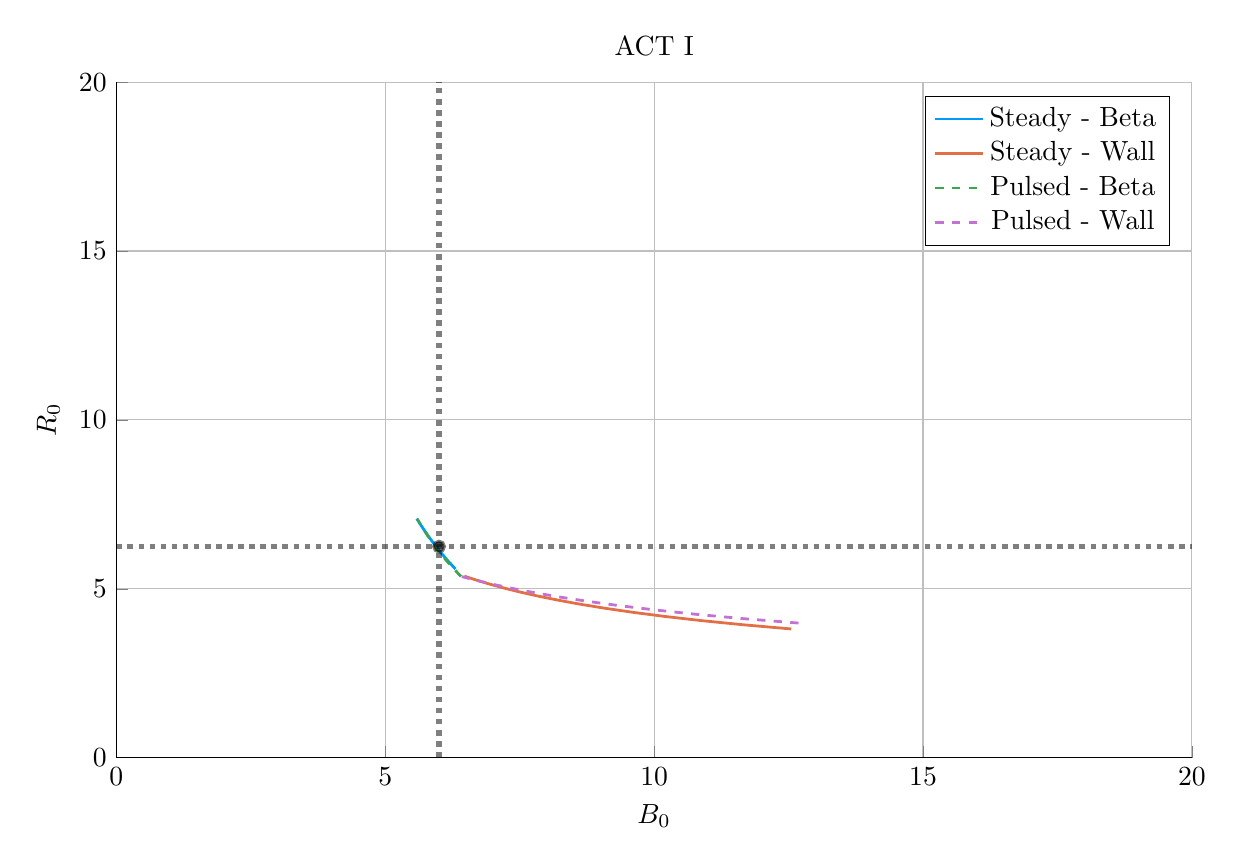
\begin{tikzpicture}[]
\begin{axis}[height = {101.6mm}, ylabel = {${R}_{0}$}, title = {ACT I}, xmin = {0.0}, xmax = {20.0}, ymax = {20.0}, xlabel = {${B}_{0}$}, {unbounded coords=jump, scaled x ticks = false, xticklabel style={rotate = 0}, xmajorgrids = true, xtick = {0.0,5.0,10.0,15.0,20.0}, xticklabels = {0,5,10,15,20}, xtick align = inside, axis lines* = left, scaled y ticks = false, yticklabel style={rotate = 0}, ymajorgrids = true, ytick = {0.0,5.0,10.0,15.0,20.0}, yticklabels = {0,5,10,15,20}, ytick align = inside, axis lines* = left,     xshift = 0.0mm,
    yshift = 0.0mm,
    axis background/.style={fill={rgb,1:red,1.00000000;green,1.00000000;blue,1.00000000}}
, colorbar style={title=}}, ymin = {0.0}, width = {152.4mm}]\addplot+ [color = {rgb,1:red,0.00000000;green,0.60560316;blue,0.97868012},
draw opacity=1.0,
line width=1,
solid,mark = none,
mark size = 2.0,
mark options = {
    color = {rgb,1:red,0.00000000;green,0.00000000;blue,0.00000000}, draw opacity = 1.0,
    fill = {rgb,1:red,0.00000000;green,0.60560316;blue,0.97868012}, fill opacity = 1.0,
    line width = 1,
    rotate = 0,
    solid
}]coordinates {
(6.30336807958207, 5.587199391496101)
(6.162193069273141, 5.831838137107903)
(6.030717178404645, 6.078157823726375)
(5.908065509576601, 6.325994353145188)
(5.793464904530972, 6.57518910191267)
(5.686229631357383, 6.825588847053452)
(5.585749511271037, 7.077045564754442)
};
\addlegendentry{Steady - Beta}
\addplot+ [color = {rgb,1:red,0.88887350;green,0.43564919;blue,0.27812294},
draw opacity=1.0,
line width=1,
solid,mark = none,
mark size = 2.0,
mark options = {
    color = {rgb,1:red,0.00000000;green,0.00000000;blue,0.00000000}, draw opacity = 1.0,
    fill = {rgb,1:red,0.88887350;green,0.43564919;blue,0.27812294}, fill opacity = 1.0,
    line width = 1,
    rotate = 0,
    solid
}]coordinates {
(12.549536249695134, 3.8108352245940957)
(11.658754653696462, 3.934083270736017)
(10.883719833507003, 4.057046546594516)
(10.206258129789394, 4.179626810883221)
(9.611335769312953, 4.301750356443285)
(9.086446934250878, 4.423366229113912)
(8.62129895070743, 4.544434218016914)
(8.207216040989662, 4.6649335402400025)
(7.837119555085499, 4.78484200403474)
(7.505047858717157, 4.9041467319817595)
(7.20604322925957, 5.022835870779136)
(6.935884710193303, 5.1409045607718795)
(6.691016583192173, 5.258349129805506)
(6.468415485086983, 5.375167957409874)
};
\addlegendentry{Steady - Wall}
\addplot+ [color = {rgb,1:red,0.24222430;green,0.64327509;blue,0.30444865},
draw opacity=1.0,
line width=1,
dashed,mark = none,
mark size = 2.0,
mark options = {
    color = {rgb,1:red,0.00000000;green,0.00000000;blue,0.00000000}, draw opacity = 1.0,
    fill = {rgb,1:red,0.24222430;green,0.64327509;blue,0.30444865}, fill opacity = 1.0,
    line width = 1,
    rotate = 0,
    solid
}]coordinates {
(6.408263337806559, 5.366131328829866)
(6.408263337806564, 5.366131328829862)
(6.385466513301022, 5.402805883604879)
(6.245492502072912, 5.638974714472524)
(6.116010320461132, 5.875875066688821)
(5.9960421481916395, 6.113307727774442)
(5.884727159112828, 6.351082733498888)
(5.781304768121868, 6.589019058920955)
(5.685100648450046, 6.826944315253105)
(5.595515000321003, 7.064694456596427)
};
\addlegendentry{Pulsed - Beta}
\addplot+ [color = {rgb,1:red,0.76444018;green,0.44411178;blue,0.82429754},
draw opacity=1.0,
line width=1,
dashed,mark = none,
mark size = 2.0,
mark options = {
    color = {rgb,1:red,0.00000000;green,0.00000000;blue,0.00000000}, draw opacity = 1.0,
    fill = {rgb,1:red,0.76444018;green,0.44411178;blue,0.82429754}, fill opacity = 1.0,
    line width = 1,
    rotate = 0,
    solid
}]coordinates {
(12.684248532650473, 3.9847907768802657)
(11.66307871570063, 4.114684512780648)
(10.781888309639141, 4.244124103742294)
(10.016282491385791, 4.373086052625054)
(9.346943280276514, 4.501549309887817)
(8.758420158941194, 4.6294950281779785)
(8.238241792953433, 4.756906348757686)
(7.776255600865612, 4.883768212546736)
(7.364131118520045, 5.010067192354689)
(6.994982564641668, 5.135791343697217)
(6.66307916140573, 5.260930071474144)
(6.408263337806559, 5.366131328829866)
(6.408263337806564, 5.366131328829862)
};
\addlegendentry{Pulsed - Wall}
\addplot+ [color = {rgb,1:red,0.00000000;green,0.00000000;blue,0.00000000},
draw opacity=0.5,
line width=2,
dotted,mark = none,
mark size = 2.0,
mark options = {
    color = {rgb,1:red,0.00000000;green,0.00000000;blue,0.00000000}, draw opacity = 0.5,
    fill = {rgb,1:red,0.00000000;green,0.00000000;blue,0.00000000}, fill opacity = 0.5,
    line width = 1,
    rotate = 0,
    solid
},forget plot]coordinates {
(0.0, 6.25)
(20.0, 6.25)
};
\addplot+ [color = {rgb,1:red,0.00000000;green,0.00000000;blue,0.00000000},
draw opacity=0.5,
line width=2,
dotted,mark = none,
mark size = 2.0,
mark options = {
    color = {rgb,1:red,0.00000000;green,0.00000000;blue,0.00000000}, draw opacity = 0.5,
    fill = {rgb,1:red,0.00000000;green,0.00000000;blue,0.00000000}, fill opacity = 0.5,
    line width = 1,
    rotate = 0,
    solid
},forget plot]coordinates {
(6.0, 0.0)
(6.0, 20.0)
};
\addplot+[draw=none, color = {rgb,1:red,0.00000000;green,0.00000000;blue,0.00000000},
draw opacity=0.5,
line width=0,
solid,mark = *,
mark size = 2.0,
mark options = {
    color = {rgb,1:red,0.00000000;green,0.00000000;blue,0.00000000}, draw opacity = 0.5,
    fill = {rgb,1:red,0.00000000;green,0.00000000;blue,0.00000000}, fill opacity = 0.5,
    line width = 1,
    rotate = 0,
    solid
},forget plot] coordinates {
(6.0, 6.25)
};
\end{axis}

\end{tikzpicture}

    \end{adjustbox}
        \caption{$R_0$ vs $B_0$}
    \end{subfigure}
    \hfill
    \begin{subfigure}[t]{0.45\textwidth}
        \centering
    \begin{adjustbox}{width=\textwidth}
      \Large
      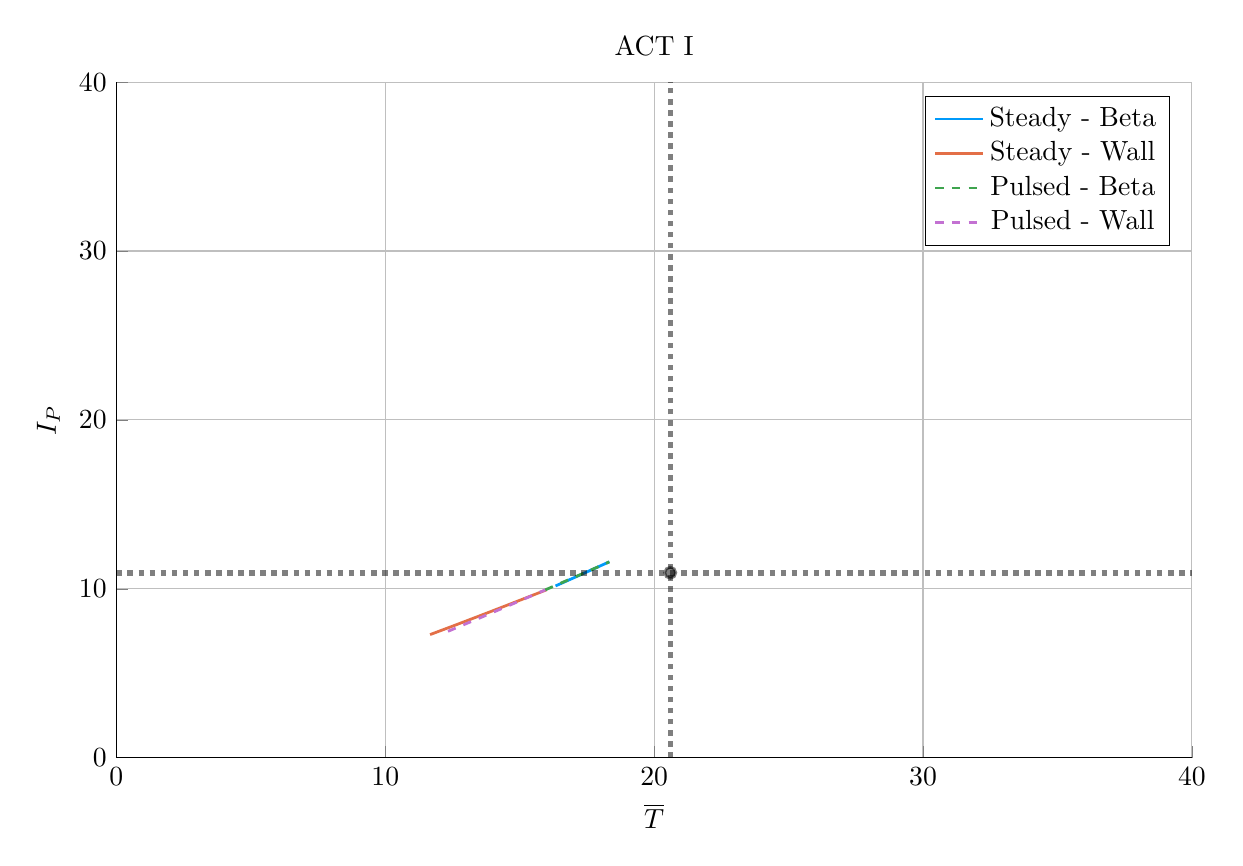
\begin{tikzpicture}[]
\begin{axis}[height = {101.6mm}, ylabel = {${I}_{P}$}, title = {ACT I}, xmin = {0.0}, xmax = {40.0}, ymax = {40.0}, xlabel = {$\overline {T}$}, {unbounded coords=jump, scaled x ticks = false, xticklabel style={rotate = 0}, xmajorgrids = true, xtick = {0.0,10.0,20.0,30.0,40.0}, xticklabels = {0,10,20,30,40}, xtick align = inside, axis lines* = left, scaled y ticks = false, yticklabel style={rotate = 0}, ymajorgrids = true, ytick = {0.0,10.0,20.0,30.0,40.0}, yticklabels = {0,10,20,30,40}, ytick align = inside, axis lines* = left,     xshift = 0.0mm,
    yshift = 0.0mm,
    axis background/.style={fill={rgb,1:red,1.00000000;green,1.00000000;blue,1.00000000}}
, colorbar style={title=}}, ymin = {0.0}, width = {152.4mm}]\addplot+ [color = {rgb,1:red,0.00000000;green,0.60560316;blue,0.97868012},
draw opacity=1.0,
line width=1,
solid,mark = none,
mark size = 2.0,
mark options = {
    color = {rgb,1:red,0.00000000;green,0.00000000;blue,0.00000000}, draw opacity = 1.0,
    fill = {rgb,1:red,0.00000000;green,0.60560316;blue,0.97868012}, fill opacity = 1.0,
    line width = 1,
    rotate = 0,
    solid
}]coordinates {
(16.333333333333332, 10.169194435531358)
(16.666666666666668, 10.405057509328124)
(17.0, 10.641905327194731)
(17.333333333333332, 10.87971637136811)
(17.666666666666668, 11.11846917050157)
(18.0, 11.358142407296011)
(18.333333333333332, 11.598714938197329)
};
\addlegendentry{Steady - Beta}
\addplot+ [color = {rgb,1:red,0.88887350;green,0.43564919;blue,0.27812294},
draw opacity=1.0,
line width=1,
solid,mark = none,
mark size = 2.0,
mark options = {
    color = {rgb,1:red,0.00000000;green,0.00000000;blue,0.00000000}, draw opacity = 1.0,
    fill = {rgb,1:red,0.88887350;green,0.43564919;blue,0.27812294}, fill opacity = 1.0,
    line width = 1,
    rotate = 0,
    solid
}]coordinates {
(11.666666666666666, 7.287903136887)
(12.0, 7.486025430610099)
(12.333333333333334, 7.685696663157812)
(12.666666666666666, 7.886645361110723)
(13.0, 8.08866940687473)
(13.333333333333334, 8.291629426976055)
(13.666666666666666, 8.495414075666067)
(14.0, 8.699964056113311)
(14.333333333333334, 8.905213556979005)
(14.666666666666666, 9.111120468746519)
(15.0, 9.31764336053339)
(15.333333333333334, 9.524758318501357)
(15.666666666666666, 9.732442959434447)
(16.0, 9.940679052729761)
};
\addlegendentry{Steady - Wall}
\addplot+ [color = {rgb,1:red,0.24222430;green,0.64327509;blue,0.30444865},
draw opacity=1.0,
line width=1,
dashed,mark = none,
mark size = 2.0,
mark options = {
    color = {rgb,1:red,0.00000000;green,0.00000000;blue,0.00000000}, draw opacity = 1.0,
    fill = {rgb,1:red,0.24222430;green,0.64327509;blue,0.30444865}, fill opacity = 1.0,
    line width = 1,
    rotate = 0,
    solid
}]coordinates {
(15.948125117373092, 9.933500150990564)
(15.9481251173731, 9.933500150990564)
(16.0, 9.969282740147014)
(16.333333333333332, 10.199548426407084)
(16.666666666666668, 10.430379144484162)
(17.0, 10.661750348679098)
(17.333333333333332, 10.893638132753678)
(17.666666666666668, 11.126019229767902)
(18.0, 11.358871009413285)
(18.333333333333332, 11.592171473618816)
};
\addlegendentry{Pulsed - Beta}
\addplot+ [color = {rgb,1:red,0.76444018;green,0.44411178;blue,0.82429754},
draw opacity=1.0,
line width=1,
dashed,mark = none,
mark size = 2.0,
mark options = {
    color = {rgb,1:red,0.00000000;green,0.00000000;blue,0.00000000}, draw opacity = 1.0,
    fill = {rgb,1:red,0.76444018;green,0.44411178;blue,0.82429754}, fill opacity = 1.0,
    line width = 1,
    rotate = 0,
    solid
}]coordinates {
(12.333333333333334, 7.481290856821823)
(12.666666666666666, 7.703549290655078)
(13.0, 7.92668121689452)
(13.333333333333334, 8.15065615613957)
(13.666666666666666, 8.375443966327172)
(14.0, 8.601014900773066)
(14.333333333333334, 8.82733966430566)
(14.666666666666666, 9.054389459546684)
(15.0, 9.282136024328327)
(15.333333333333334, 9.510551661584085)
(15.666666666666666, 9.73960926266661)
(15.948125117373092, 9.933500150990564)
(15.9481251173731, 9.933500150990564)
};
\addlegendentry{Pulsed - Wall}
\addplot+ [color = {rgb,1:red,0.00000000;green,0.00000000;blue,0.00000000},
draw opacity=0.5,
line width=2,
dotted,mark = none,
mark size = 2.0,
mark options = {
    color = {rgb,1:red,0.00000000;green,0.00000000;blue,0.00000000}, draw opacity = 0.5,
    fill = {rgb,1:red,0.00000000;green,0.00000000;blue,0.00000000}, fill opacity = 0.5,
    line width = 1,
    rotate = 0,
    solid
},forget plot]coordinates {
(0.0, 10.95)
(40.0, 10.95)
};
\addplot+ [color = {rgb,1:red,0.00000000;green,0.00000000;blue,0.00000000},
draw opacity=0.5,
line width=2,
dotted,mark = none,
mark size = 2.0,
mark options = {
    color = {rgb,1:red,0.00000000;green,0.00000000;blue,0.00000000}, draw opacity = 0.5,
    fill = {rgb,1:red,0.00000000;green,0.00000000;blue,0.00000000}, fill opacity = 0.5,
    line width = 1,
    rotate = 0,
    solid
},forget plot]coordinates {
(20.6, 0.0)
(20.6, 40.0)
};
\addplot+[draw=none, color = {rgb,1:red,0.00000000;green,0.00000000;blue,0.00000000},
draw opacity=0.5,
line width=0,
solid,mark = *,
mark size = 2.0,
mark options = {
    color = {rgb,1:red,0.00000000;green,0.00000000;blue,0.00000000}, draw opacity = 0.5,
    fill = {rgb,1:red,0.00000000;green,0.00000000;blue,0.00000000}, fill opacity = 0.5,
    line width = 1,
    rotate = 0,
    solid
},forget plot] coordinates {
(20.6, 10.95)
};
\end{axis}

\end{tikzpicture}

    \end{adjustbox}
        \caption{$I_P$ vs $\overline T$}
    \end{subfigure}
    \hfill \hfill ~\\ ~\\ ~\\
    \caption{Aries Act I Model Comparison} ~\\
\end{figure*}

\begin{table}[h!]
\centering  
\caption{Act I Variables}
\hfill
\begin{subtable}[t]{0.4\textwidth}
\centering  
\caption{Input Variables} ~\\
\begin{tabular}{ c|c } 

Input            & Value           \\
\hline
$H$              & 1.65            \\
$Q$              & 42.5            \\
$N_{G}$          & 1.0             \\
$\epsilon$       & 0.25            \\
$\kappa_{95}$    & 2.1             \\
$\delta_{95}$    & 0.4             \\
$\nu_{n}$        & 0.27            \\
$\nu_{T}$        & 1.15            \\
$l_{i}$          & 0.359         \\
$A$              & 2.5             \\
$Z_{eff}$        & 2.11            \\
$f_{D}$          & 0.75            \\
$\tau_{FT}$      & 1.6e9           \\
$B_{CS}$         & 12.77           \\

\end{tabular}
\end{subtable}
\hfill
\begin{subtable}[t]{0.5\textwidth}
\centering  
\caption{Output Variables} ~\\
\begin{tabular}{ c|c|c } 

Output           & Original         & Fussy.jl        \\
\hline
$R_{0}$          & 6.25             & 6.23           \\
$B_{0}$          & 6.0              & 6.0           \\
$I_{P}$          & 10.95            & 10.78           \\
$\overline n$    & 1.3              & 1.3           \\
$\overline T$    & 20.6             & 17.2            \\
$\beta_{N}$       & 0.0427           & -          \\
$q_{95}$         & 4.5              & 4.0           \\
$P_{W}$          & 2.45             & 2.00           \\
$f_{BS}$         & 0.91             & 0.91           \\
$f_{CD}$         & 0.09             & 0.09           \\
$f_{ID}$         & -              & -             \\
$\volume$         & 582.0            & 621.4           \\
$P_{F}$          & 1813           & 1865          \\
$\eta_{CD}$      & 0.188            & 0.185          \\

\end{tabular}
\end{subtable}
\hfill
\hfill
\end{table}

\newpage 

\subsubsection{Act II -- Conservative Physics and Engineering}

ARIES more conservative design -- Act II -- is much more like ARC in nature. From the plots, it is obvious the paper's model is basically right on top of the reactor curve made using Fussy.jl.  Much like ARC, too, it shows how the model overestimates fusion power and underestimates bootstrap fraction due to their selection of a pedestal profile for plasma temperature.

\begin{figure*}[h!]
    \centering
    \hfill 
    \begin{subfigure}[t]{0.45\textwidth}
        \centering
    \begin{adjustbox}{width=\textwidth}
      \Large
      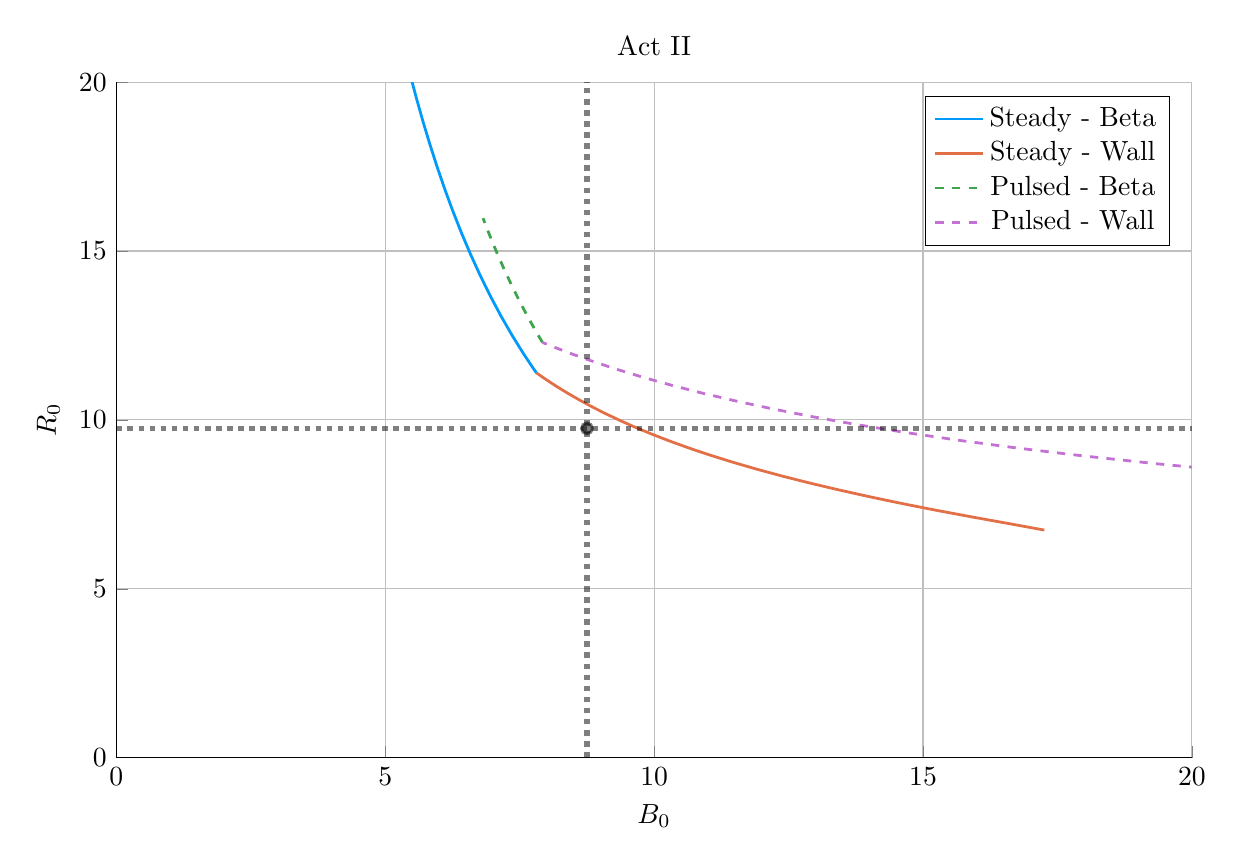
\begin{tikzpicture}[]
\begin{axis}[height = {101.6mm}, ylabel = {${R}_{0}$}, title = {Act II}, xmin = {0.0}, xmax = {20.0}, ymax = {20.0}, xlabel = {${B}_{0}$}, {unbounded coords=jump, scaled x ticks = false, xticklabel style={rotate = 0}, xmajorgrids = true, xtick = {0.0,5.0,10.0,15.0,20.0}, xticklabels = {0,5,10,15,20}, xtick align = inside, axis lines* = left, scaled y ticks = false, yticklabel style={rotate = 0}, ymajorgrids = true, ytick = {0.0,5.0,10.0,15.0,20.0}, yticklabels = {0,5,10,15,20}, ytick align = inside, axis lines* = left,     xshift = 0.0mm,
    yshift = 0.0mm,
    axis background/.style={fill={rgb,1:red,1.00000000;green,1.00000000;blue,1.00000000}}
, colorbar style={title=}}, ymin = {0.0}, width = {152.4mm}]\addplot+ [color = {rgb,1:red,0.00000000;green,0.60560316;blue,0.97868012},
draw opacity=1.0,
line width=1,
solid,mark = none,
mark size = 2.0,
mark options = {
    color = {rgb,1:red,0.00000000;green,0.00000000;blue,0.00000000}, draw opacity = 1.0,
    fill = {rgb,1:red,0.00000000;green,0.60560316;blue,0.97868012}, fill opacity = 1.0,
    line width = 1,
    rotate = 0,
    solid
}]coordinates {
(7.810935944285959, 11.389141268081966)
(7.57736049850867, 11.942634046586162)
(7.354864292609041, 12.51245847357923)
(7.145167234136329, 13.0943365692581)
(6.9473303865083675, 13.687993788149779)
(6.760499508614096, 14.293145886478186)
(6.583897990324067, 14.909495325365516)
(6.416817229618043, 15.536734694045393)
(6.258609820663305, 16.1745467994937)
(6.108683264880386, 16.82260538899235)
(5.966494431410919, 17.480575868750975)
(5.831544666176381, 18.148116014600475)
(5.703375459679132, 18.824876684423757)
(5.581564609582325, 19.510502502077443)
(5.465722802994068, 20.20463254880097)
(5.355490573482678, 20.906901035327614)
(5.25053558682053, 21.616937949657327)
(5.1505502068221745, 22.334369714080776)
(5.0552493196883175, 23.058819802110854)
};
\addlegendentry{Steady - Beta}
\addplot+ [color = {rgb,1:red,0.88887350;green,0.43564919;blue,0.27812294},
draw opacity=1.0,
line width=1,
solid,mark = none,
mark size = 2.0,
mark options = {
    color = {rgb,1:red,0.00000000;green,0.00000000;blue,0.00000000}, draw opacity = 1.0,
    fill = {rgb,1:red,0.88887350;green,0.43564919;blue,0.27812294}, fill opacity = 1.0,
    line width = 1,
    rotate = 0,
    solid
}]coordinates {
(17.25550839059296, 6.738604635617289)
(16.594334962335296, 6.931178286222189)
(15.9071755430688, 7.128187388035985)
(15.233983138507648, 7.327817939330552)
(14.594239858921854, 7.528927553154291)
(13.989673082630297, 7.7312042898700515)
(13.414782495717416, 7.934790159202381)
(12.872659546281994, 8.139273115071695)
(12.364365715508608, 8.344321605506495)
(11.889507953196574, 8.549679244077495)
(11.44685939646348, 8.755144058838903)
(11.034739998180656, 8.960554762148757)
(10.651252523287319, 9.165781242855727)
(10.294428800132035, 9.370717743724994)
(9.962319203963213, 9.57527782549947)
(9.653045819449929, 9.779390564591205)
(9.364832254395445, 9.982997628553138)
(9.096018465506306, 10.186050992034668)
(8.844373144802077, 10.388606525997883)
(8.61055754360846, 10.590345571972314)
(8.391192178573277, 10.791527736428888)
(8.18577947665566, 10.992035979756642)
(7.99323348423048, 11.1918525509058)
(7.812301489248497, 11.391007917726574)
};
\addlegendentry{Steady - Wall}
\addplot+ [color = {rgb,1:red,0.24222430;green,0.64327509;blue,0.30444865},
draw opacity=1.0,
line width=1,
dashed,mark = none,
mark size = 2.0,
mark options = {
    color = {rgb,1:red,0.00000000;green,0.00000000;blue,0.00000000}, draw opacity = 1.0,
    fill = {rgb,1:red,0.24222430;green,0.64327509;blue,0.30444865}, fill opacity = 1.0,
    line width = 1,
    rotate = 0,
    solid
}]coordinates {
(7.923668284887995, 12.293879059492616)
(7.923668284887995, 12.293879059492635)
(7.836759696043437, 12.52591633746021)
(7.6662731560983355, 13.00454403942661)
(7.50499428233835, 13.488375025456907)
(7.35232773269976, 13.977065733125242)
(7.207727224738343, 14.470269937628656)
(7.070690693175276, 14.967639476613451)
(6.940756001029682, 15.46882496625731)
(6.817497143644154, 15.973476480630131)
};
\addlegendentry{Pulsed - Beta}
\addplot+ [color = {rgb,1:red,0.76444018;green,0.44411178;blue,0.82429754},
draw opacity=1.0,
line width=1,
dashed,mark = none,
mark size = 2.0,
mark options = {
    color = {rgb,1:red,0.00000000;green,0.00000000;blue,0.00000000}, draw opacity = 1.0,
    fill = {rgb,1:red,0.76444018;green,0.44411178;blue,0.82429754}, fill opacity = 1.0,
    line width = 1,
    rotate = 0,
    solid
}]coordinates {
(22.56106430311702, 8.239911323116141)
(20.85607192394036, 8.471453471694678)
(19.335265246056654, 8.703260993170346)
(17.974121547130903, 8.935277031603567)
(16.751976718553127, 9.167446093344447)
(15.651329744019142, 9.399714010238458)
(14.65728744097675, 9.632027927077594)
(13.757118584462601, 9.864336290607328)
(12.939893642194303, 10.096588839007167)
(12.196191964860315, 10.328736591776112)
(11.517862472405039, 10.560731839999896)
(10.897827027335556, 10.792528137074703)
(10.329918077124672, 11.02408028901105)
(9.808743940706389, 11.255344346143936)
(9.329576544487265, 11.486277593626015)
(8.888257451278507, 11.716838542453242)
(8.481118883411932, 11.946986920205564)
(8.10491708701527, 12.17668366154026)
(7.923668284887995, 12.293879059492616)
(7.923668284887995, 12.293879059492635)
};
\addlegendentry{Pulsed - Wall}
\addplot+ [color = {rgb,1:red,0.00000000;green,0.00000000;blue,0.00000000},
draw opacity=0.5,
line width=2,
dotted,mark = none,
mark size = 2.0,
mark options = {
    color = {rgb,1:red,0.00000000;green,0.00000000;blue,0.00000000}, draw opacity = 0.5,
    fill = {rgb,1:red,0.00000000;green,0.00000000;blue,0.00000000}, fill opacity = 0.5,
    line width = 1,
    rotate = 0,
    solid
},forget plot]coordinates {
(0.0, 9.75)
(20.0, 9.75)
};
\addplot+ [color = {rgb,1:red,0.00000000;green,0.00000000;blue,0.00000000},
draw opacity=0.5,
line width=2,
dotted,mark = none,
mark size = 2.0,
mark options = {
    color = {rgb,1:red,0.00000000;green,0.00000000;blue,0.00000000}, draw opacity = 0.5,
    fill = {rgb,1:red,0.00000000;green,0.00000000;blue,0.00000000}, fill opacity = 0.5,
    line width = 1,
    rotate = 0,
    solid
},forget plot]coordinates {
(8.75, 0.0)
(8.75, 20.0)
};
\addplot+[draw=none, color = {rgb,1:red,0.00000000;green,0.00000000;blue,0.00000000},
draw opacity=0.5,
line width=0,
solid,mark = *,
mark size = 2.0,
mark options = {
    color = {rgb,1:red,0.00000000;green,0.00000000;blue,0.00000000}, draw opacity = 0.5,
    fill = {rgb,1:red,0.00000000;green,0.00000000;blue,0.00000000}, fill opacity = 0.5,
    line width = 1,
    rotate = 0,
    solid
},forget plot] coordinates {
(8.75, 9.75)
};
\end{axis}

\end{tikzpicture}

    \end{adjustbox}
        \caption{$R_0$ vs $B_0$}
    \end{subfigure}
    \hfill
    \begin{subfigure}[t]{0.45\textwidth}
        \centering
    \begin{adjustbox}{width=\textwidth}
      \Large
      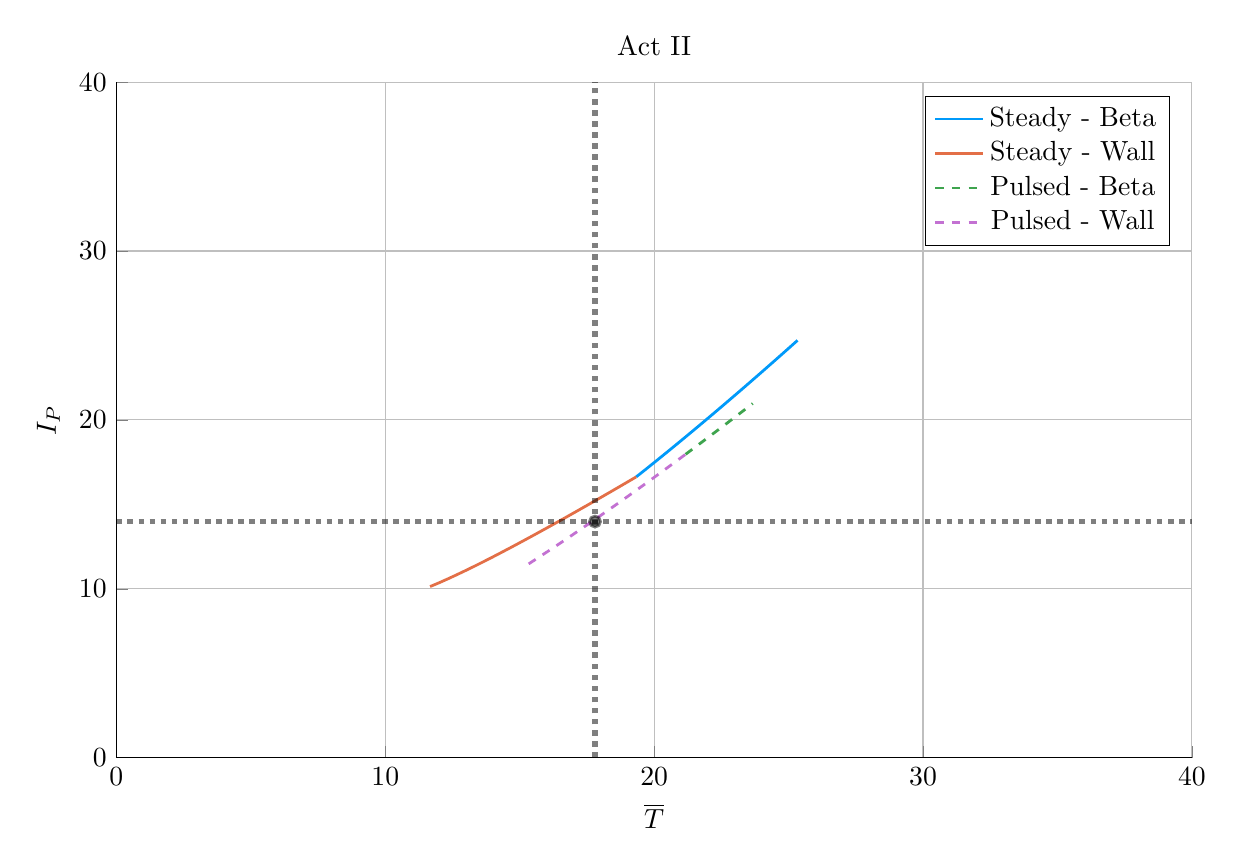
\begin{tikzpicture}[]
\begin{axis}[height = {101.6mm}, ylabel = {${I}_{P}$}, title = {Act II}, xmin = {0.0}, xmax = {40.0}, ymax = {40.0}, xlabel = {$\overline {T}$}, {unbounded coords=jump, scaled x ticks = false, xticklabel style={rotate = 0}, xmajorgrids = true, xtick = {0.0,10.0,20.0,30.0,40.0}, xticklabels = {0,10,20,30,40}, xtick align = inside, axis lines* = left, scaled y ticks = false, yticklabel style={rotate = 0}, ymajorgrids = true, ytick = {0.0,10.0,20.0,30.0,40.0}, yticklabels = {0,10,20,30,40}, ytick align = inside, axis lines* = left,     xshift = 0.0mm,
    yshift = 0.0mm,
    axis background/.style={fill={rgb,1:red,1.00000000;green,1.00000000;blue,1.00000000}}
, colorbar style={title=}}, ymin = {0.0}, width = {152.4mm}]\addplot+ [color = {rgb,1:red,0.00000000;green,0.60560316;blue,0.97868012},
draw opacity=1.0,
line width=1,
solid,mark = none,
mark size = 2.0,
mark options = {
    color = {rgb,1:red,0.00000000;green,0.00000000;blue,0.00000000}, draw opacity = 1.0,
    fill = {rgb,1:red,0.00000000;green,0.60560316;blue,0.97868012}, fill opacity = 1.0,
    line width = 1,
    rotate = 0,
    solid
}]coordinates {
(19.333333333333332, 16.626976584120992)
(19.666666666666668, 17.04714126565062)
(20.0, 17.4728205159228)
(20.333333333333332, 17.902037802268676)
(20.666666666666668, 18.334710756318135)
(21.0, 18.770758343299946)
(21.333333333333332, 19.21009903030823)
(21.666666666666668, 19.652652028291016)
(22.0, 20.098337062332053)
(22.333333333333332, 20.547074418426956)
(22.666666666666668, 20.998784986741654)
(23.0, 21.453390301179443)
(23.333333333333332, 21.910812577709113)
(23.666666666666668, 22.37097474604109)
(24.0, 22.833800482195542)
(24.333333333333332, 23.299214237115898)
(24.666666666666668, 23.767141260842724)
(25.0, 24.237507628970306)
(25.333333333333332, 24.710240262329886)
};
\addlegendentry{Steady - Beta}
\addplot+ [color = {rgb,1:red,0.88887350;green,0.43564919;blue,0.27812294},
draw opacity=1.0,
line width=1,
solid,mark = none,
mark size = 2.0,
mark options = {
    color = {rgb,1:red,0.00000000;green,0.00000000;blue,0.00000000}, draw opacity = 1.0,
    fill = {rgb,1:red,0.88887350;green,0.43564919;blue,0.27812294}, fill opacity = 1.0,
    line width = 1,
    rotate = 0,
    solid
}]coordinates {
(11.666666666666666, 10.131702672149428)
(12.0, 10.354462623384137)
(12.333333333333334, 10.591104956642406)
(12.666666666666666, 10.837356598740662)
(13.0, 11.09054386610192)
(13.333333333333334, 11.349883742416331)
(13.666666666666666, 11.61561327802365)
(14.0, 11.886764241828663)
(14.333333333333334, 12.16256217004895)
(14.666666666666666, 12.44240841774136)
(15.0, 12.72583049098312)
(15.333333333333334, 13.012449288635679)
(15.666666666666666, 13.301956539143166)
(16.0, 13.59409872387861)
(16.333333333333332, 13.888665310111481)
(16.666666666666668, 14.185479949266789)
(17.0, 14.48439377498311)
(17.333333333333332, 14.785280223642218)
(17.666666666666668, 15.088238807947413)
(18.0, 15.392552774473998)
(18.333333333333332, 15.698764813772398)
(18.666666666666668, 16.00659672680533)
(19.0, 16.315986303185774)
(19.333333333333332, 16.626976584120992)
};
\addlegendentry{Steady - Wall}
\addplot+ [color = {rgb,1:red,0.24222430;green,0.64327509;blue,0.30444865},
draw opacity=1.0,
line width=1,
dashed,mark = none,
mark size = 2.0,
mark options = {
    color = {rgb,1:red,0.00000000;green,0.00000000;blue,0.00000000}, draw opacity = 1.0,
    fill = {rgb,1:red,0.24222430;green,0.64327509;blue,0.30444865}, fill opacity = 1.0,
    line width = 1,
    rotate = 0,
    solid
}]coordinates {
(21.17034352159018, 17.96627417153032)
(21.170343521590212, 17.966274171530337)
(21.333333333333332, 18.1591936305205)
(21.666666666666668, 18.555297107283753)
(22.0, 18.953426399022014)
(22.333333333333332, 19.353497539767794)
(22.666666666666668, 19.7554274455778)
(23.0, 20.159133974954596)
(23.333333333333332, 20.564535986760628)
(23.666666666666668, 20.971553389451927)
};
\addlegendentry{Pulsed - Beta}
\addplot+ [color = {rgb,1:red,0.76444018;green,0.44411178;blue,0.82429754},
draw opacity=1.0,
line width=1,
dashed,mark = none,
mark size = 2.0,
mark options = {
    color = {rgb,1:red,0.00000000;green,0.00000000;blue,0.00000000}, draw opacity = 1.0,
    fill = {rgb,1:red,0.76444018;green,0.44411178;blue,0.82429754}, fill opacity = 1.0,
    line width = 1,
    rotate = 0,
    solid
}]coordinates {
(15.333333333333334, 11.474678053719876)
(15.666666666666666, 11.819475032994422)
(16.0, 12.167858357397087)
(16.333333333333332, 12.51974460671026)
(16.666666666666668, 12.875049128346197)
(17.0, 13.233686175102404)
(17.333333333333332, 13.595569077154208)
(17.666666666666668, 13.96061040317257)
(18.0, 14.328722110173729)
(18.333333333333332, 14.699815683529526)
(18.666666666666668, 15.073802268415148)
(19.0, 15.450592793824576)
(19.333333333333332, 15.830098089115069)
(19.666666666666668, 16.21222899561205)
(20.0, 16.596896471191773)
(20.333333333333332, 16.984011690059134)
(20.666666666666668, 17.37348613728185)
(21.0, 17.765231698435688)
(21.17034352159018, 17.96627417153032)
(21.170343521590212, 17.966274171530337)
};
\addlegendentry{Pulsed - Wall}
\addplot+ [color = {rgb,1:red,0.00000000;green,0.00000000;blue,0.00000000},
draw opacity=0.5,
line width=2,
dotted,mark = none,
mark size = 2.0,
mark options = {
    color = {rgb,1:red,0.00000000;green,0.00000000;blue,0.00000000}, draw opacity = 0.5,
    fill = {rgb,1:red,0.00000000;green,0.00000000;blue,0.00000000}, fill opacity = 0.5,
    line width = 1,
    rotate = 0,
    solid
},forget plot]coordinates {
(0.0, 13.98)
(40.0, 13.98)
};
\addplot+ [color = {rgb,1:red,0.00000000;green,0.00000000;blue,0.00000000},
draw opacity=0.5,
line width=2,
dotted,mark = none,
mark size = 2.0,
mark options = {
    color = {rgb,1:red,0.00000000;green,0.00000000;blue,0.00000000}, draw opacity = 0.5,
    fill = {rgb,1:red,0.00000000;green,0.00000000;blue,0.00000000}, fill opacity = 0.5,
    line width = 1,
    rotate = 0,
    solid
},forget plot]coordinates {
(17.8, 0.0)
(17.8, 40.0)
};
\addplot+[draw=none, color = {rgb,1:red,0.00000000;green,0.00000000;blue,0.00000000},
draw opacity=0.5,
line width=0,
solid,mark = *,
mark size = 2.0,
mark options = {
    color = {rgb,1:red,0.00000000;green,0.00000000;blue,0.00000000}, draw opacity = 0.5,
    fill = {rgb,1:red,0.00000000;green,0.00000000;blue,0.00000000}, fill opacity = 0.5,
    line width = 1,
    rotate = 0,
    solid
},forget plot] coordinates {
(17.8, 13.98)
};
\end{axis}

\end{tikzpicture}

    \end{adjustbox}
        \caption{$I_P$ vs $\overline T$}
    \end{subfigure}
    \hfill \hfill ~\\ ~\\ ~\\
    \caption{Aries Act II Model Comparison} ~\\
\end{figure*}

\begin{table}[h!]
\centering  
\caption{Act II Variables}
\hfill
\begin{subtable}[t]{0.4\textwidth}
\centering  
\caption{Input Variables} ~\\
\begin{tabular}{ c|c } 

Input            & Value           \\
\hline
$H$              & 1.22            \\
$Q$              & 25.0            \\
$N_{G}$          & 1.3             \\
$\epsilon$       & 0.25            \\
$\kappa_{95}$    & 1.964           \\
$\delta_{95}$    & 0.42            \\
$\nu_{n}$        & 0.41            \\
$\nu_{T}$        & 1.15            \\
$l_{i}$          & 0.60275         \\
$A$              & 2.5             \\
$Z_{eff}$        & 2.12            \\
$f_{D}$          & 0.74            \\
$\tau_{FT}$      & 1.6e9           \\
$B_{CS}$         & 12.77           \\

\end{tabular}
\end{subtable}
\hfill
\begin{subtable}[t]{0.5\textwidth}
\centering  
\caption{Output Variables} ~\\
\begin{tabular}{ c|c|c } 

Output           & Original         & Fussy.jl        \\
\hline
$R_{0}$          & 9.75             & 10.22           \\
$B_{0}$          & 8.75             & 9.05           \\
$I_{P}$          & 13.98            & 14.84           \\
$\overline n$    & 0.86             & 0.82          \\
$\overline T$    & 17.8             & 17.4           \\
$\beta_{N}$       & 0.026            & 0.023          \\
$q_{95}$         & 8.0              & 6.6           \\
$P_{W}$          & 1.46             & -            \\
$f_{BS}$         & 0.77             & 0.66           \\
$f_{CD}$         & 0.23             & 0.34           \\
$f_{ID}$         & -              & -             \\
$\volume$         & 2209           & 2559          \\
$P_{F}$          & 2637           & 3460          \\
$\eta_{CD}$      & 0.256            & 0.307           \\

\end{tabular}
\end{subtable}
\hfill
\hfill
\end{table}

\newpage

\subsection{Benchmarking with the Process DEMO Designs}

The PROCESS team's prospective designs for successors to ITER constitute the final set of model comparisons: the steady-state and pulsed DEMO reactors. As this paper is designed to compare these modes of operation, this study proves most fruitful. It also highlights how common model decisions can dramatically alter what reactors come out of the solvers.

The first discrepancy is how the PROCESS team defines the loss term in the ELMy H-Mode scaling law. As shown in their paper, they actually subtract out a Bremsstrahlung component, while leaving the fitting coefficients the same. \cite{process} After modifying Fussy.jl to incorporate this definition, the steady-state reactor is easily reproducible in $R_0$ -- $B_0$ slice of reactor space.

Unlike the steady-state case, however, the modified power loss term does not fix the pulsed case, as it actually draws the reactor curves further from the design in their paper. As such, it is flux balance that is now the main culprit for discrepencies between the two models. This makes sense, as this model uses highly simplified source terms -- namely neglecting anything but the central solenoid and PF coils (as well as ignoring crucial physics for these two components). Even acknowledging the differences between the two models, Fussy.jl still does remarkably well at reproducing their much more sophisticated coding framework. 

The final point to make is about selecting optimum points to build as the \replaced{dynamic}{floating} variables are allowed to make curves through reactor space. Up to this point, only steady-state tokamak designs have been explored. In every single one of these, though, the paper values have been very close to the point where the beta curves and wall loading curves cross. This is because they all result in the minimum cost-per-watt. 

For pulsed designs, on the other hand, kink curves start to appear for low magnetic field strengths. Just as beta-wall intersections were optimum places to design for low cost-per-watt ($C_W$) reactors, these beta-kink intersections will prove to be the place where minimum capital cost ($W_M$) reactors usually occur.

\newpage 

\subsubsection{DEMO Steady -- A Steady-State ITER Successor}

Hands down, this DEMO Steady reactor is the worst modeled reactor using Fussy.jl. As mentioned previously, though, some of the discrepancy was removed by using the PROCESS team's modified version of heat loss. This heavily corrected the $R_0$ -- $B_0$ curve, but had no effect on the $I_P$ -- $\overline T$ one. An interesting aside is that these curves actually show how steady current is independent of \replaced{limiting}{secondary} constraint (as noted).

\begin{figure*}[h!]
    \centering
    \hfill 
    \begin{subfigure}[t]{0.45\textwidth}
        \centering
    \begin{adjustbox}{width=\textwidth}
      \Large
      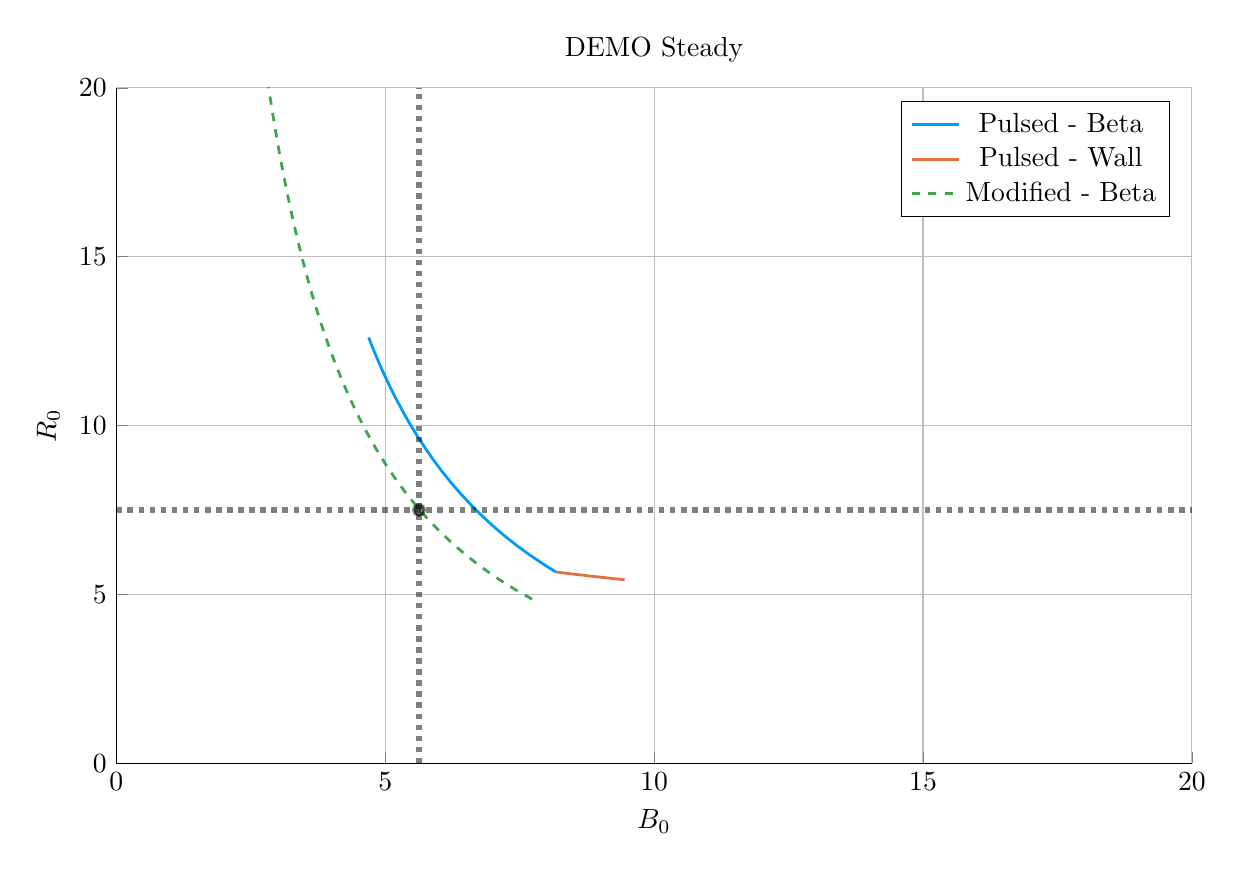
\begin{tikzpicture}[]
\begin{axis}[height = {101.6mm}, ylabel = {${R}_{0}$}, title = {DEMO Steady}, xmin = {0.0}, xmax = {20.0}, ymax = {20.0}, xlabel = {${B}_{0}$}, {unbounded coords=jump, scaled x ticks = false, xticklabel style={rotate = 0}, xmajorgrids = true, xtick = {0.0,5.0,10.0,15.0,20.0}, xticklabels = {0,5,10,15,20}, xtick align = inside, axis lines* = left, scaled y ticks = false, yticklabel style={rotate = 0}, ymajorgrids = true, ytick = {0.0,5.0,10.0,15.0,20.0}, yticklabels = {0,5,10,15,20}, ytick align = inside, axis lines* = left,     xshift = 0.0mm,
    yshift = 0.0mm,
    axis background/.style={fill={rgb,1:red,1.00000000;green,1.00000000;blue,1.00000000}}
, colorbar style={title=}}, ymin = {0.0}, width = {152.4mm}]\addplot+ [color = {rgb,1:red,0.00000000;green,0.60560316;blue,0.97868012},
draw opacity=1.0,
line width=1,
solid,mark = none,
mark size = 2.0,
mark options = {
    color = {rgb,1:red,0.00000000;green,0.00000000;blue,0.00000000}, draw opacity = 1.0,
    fill = {rgb,1:red,0.00000000;green,0.60560316;blue,0.97868012}, fill opacity = 1.0,
    line width = 1,
    rotate = 0,
    solid
}]coordinates {
(8.173486873088942, 5.664794455960266)
(7.942780080136996, 5.894389477908349)
(7.682110747013332, 6.174587309854596)
(7.436076373351653, 6.4617259587740365)
(7.203701032854224, 6.7556817964635885)
(6.984087846006315, 7.056316762210614)
(6.776411507024863, 7.363478485110443)
(6.579911624110169, 7.677000456183209)
(6.393886772782909, 7.996702249919802)
(6.217689175869905, 8.322389794615686)
(6.050719935402341, 8.653855690575247)
(5.892424751644716, 8.990879574996331)
(5.742290072962272, 9.333228532083597)
(5.599839627496144, 9.680657546690735)
(5.464631293842628, 10.03290999955685)
(5.33625427328881, 10.389718201981736)
(5.214326530771975, 10.75080396758328)
(5.098492475718857, 11.115879218594692)
(4.98842085737482, 11.484646623994054)
(4.88380285223036, 11.85680026661456)
(4.784350323760147, 12.232026336259217)
(4.689794236961777, 12.610003845742904)
};
\addlegendentry{Pulsed - Beta}
\addplot+ [color = {rgb,1:red,0.88887350;green,0.43564919;blue,0.27812294},
draw opacity=1.0,
line width=1,
solid,mark = none,
mark size = 2.0,
mark options = {
    color = {rgb,1:red,0.00000000;green,0.00000000;blue,0.00000000}, draw opacity = 1.0,
    fill = {rgb,1:red,0.88887350;green,0.43564919;blue,0.27812294}, fill opacity = 1.0,
    line width = 1,
    rotate = 0,
    solid
}]coordinates {
(9.452194760190558, 5.436039445052516)
(8.82895875946862, 5.541751345019407)
(8.260410483462291, 5.64769543408014)
(8.173486873088942, 5.664794455960266)
};
\addlegendentry{Pulsed - Wall}
\addplot+ [color = {rgb,1:red,0.24222430;green,0.64327509;blue,0.30444865},
draw opacity=1.0,
line width=1,
dashed,mark = none,
mark size = 2.0,
mark options = {
    color = {rgb,1:red,0.00000000;green,0.00000000;blue,0.00000000}, draw opacity = 1.0,
    fill = {rgb,1:red,0.24222430;green,0.64327509;blue,0.30444865}, fill opacity = 1.0,
    line width = 1,
    rotate = 0,
    solid
}]coordinates {
(7.729015258613306, 4.861871150043874)
(7.398090906424027, 5.162615732748398)
(7.087604971989989, 5.475689582149146)
(6.796029845186129, 5.801261884855786)
(6.5219747916377235, 6.139486028413868)
(6.264171517105504, 6.490498735804173)
(6.021461495247516, 6.854419238072999)
(5.792784817023639, 7.231348485954994)
(5.57717035299729, 7.621368405021026)
(5.3737270519036775, 8.024541198865679)
(5.1816362256187425, 8.440908704652248)
(5.000144692923053, 8.870491805097014)
(4.828558673035444, 9.313289900712723)
(4.666238335465348, 9.769280445839089)
(4.512592925835539, 10.23841855166636)
(4.367076398389423, 10.720636659108127)
(4.229183495269078, 11.215844284001262)
(4.098446220614958, 11.723927836706606)
(3.974430664327246, 12.244750517759236)
(3.856734136133517, 12.778152290770123)
(3.744982575583214, 13.323949933321568)
(3.6388282078672565, 13.881937166125676)
(3.537947419047361, 14.45188486023713)
(3.4420388274654035, 15.033541321628862)
(3.3508215308612357, 15.626632651963563)
(3.2640335111230074, 16.230863183919308)
(3.18143018067718, 16.84591598897328)
(3.1027830563428513, 17.471453455103656)
(3.0278785480626333, 18.107117931452404)
(2.956516851312625, 18.752532436599008)
(2.888510933213844, 19.407301426734122)
(2.823685603439882, 20.071011619694055)
(2.761876661959762, 20.74323287052923)
(2.702930116488407, 21.423519094029906)
(2.646701463253573, 22.111409229427537)
(2.593055025340143, 22.806428242329144)
};
\addlegendentry{Modified - Beta}
\addplot+ [color = {rgb,1:red,0.00000000;green,0.00000000;blue,0.00000000},
draw opacity=0.5,
line width=2,
dotted,mark = none,
mark size = 2.0,
mark options = {
    color = {rgb,1:red,0.00000000;green,0.00000000;blue,0.00000000}, draw opacity = 0.5,
    fill = {rgb,1:red,0.00000000;green,0.00000000;blue,0.00000000}, fill opacity = 0.5,
    line width = 1,
    rotate = 0,
    solid
},forget plot]coordinates {
(0.0, 7.5)
(20.0, 7.5)
};
\addplot+ [color = {rgb,1:red,0.00000000;green,0.00000000;blue,0.00000000},
draw opacity=0.5,
line width=2,
dotted,mark = none,
mark size = 2.0,
mark options = {
    color = {rgb,1:red,0.00000000;green,0.00000000;blue,0.00000000}, draw opacity = 0.5,
    fill = {rgb,1:red,0.00000000;green,0.00000000;blue,0.00000000}, fill opacity = 0.5,
    line width = 1,
    rotate = 0,
    solid
},forget plot]coordinates {
(5.627, 0.0)
(5.627, 20.0)
};
\addplot+[draw=none, color = {rgb,1:red,0.00000000;green,0.00000000;blue,0.00000000},
draw opacity=0.5,
line width=0,
solid,mark = *,
mark size = 2.0,
mark options = {
    color = {rgb,1:red,0.00000000;green,0.00000000;blue,0.00000000}, draw opacity = 0.5,
    fill = {rgb,1:red,0.00000000;green,0.00000000;blue,0.00000000}, fill opacity = 0.5,
    line width = 1,
    rotate = 0,
    solid
},forget plot] coordinates {
(5.627, 7.5)
};
\end{axis}

\end{tikzpicture}

    \end{adjustbox}
        \caption{$R_0$ vs $B_0$}
    \end{subfigure}
    \hfill
    \begin{subfigure}[t]{0.45\textwidth}
        \centering
    \begin{adjustbox}{width=\textwidth}
      \Large
      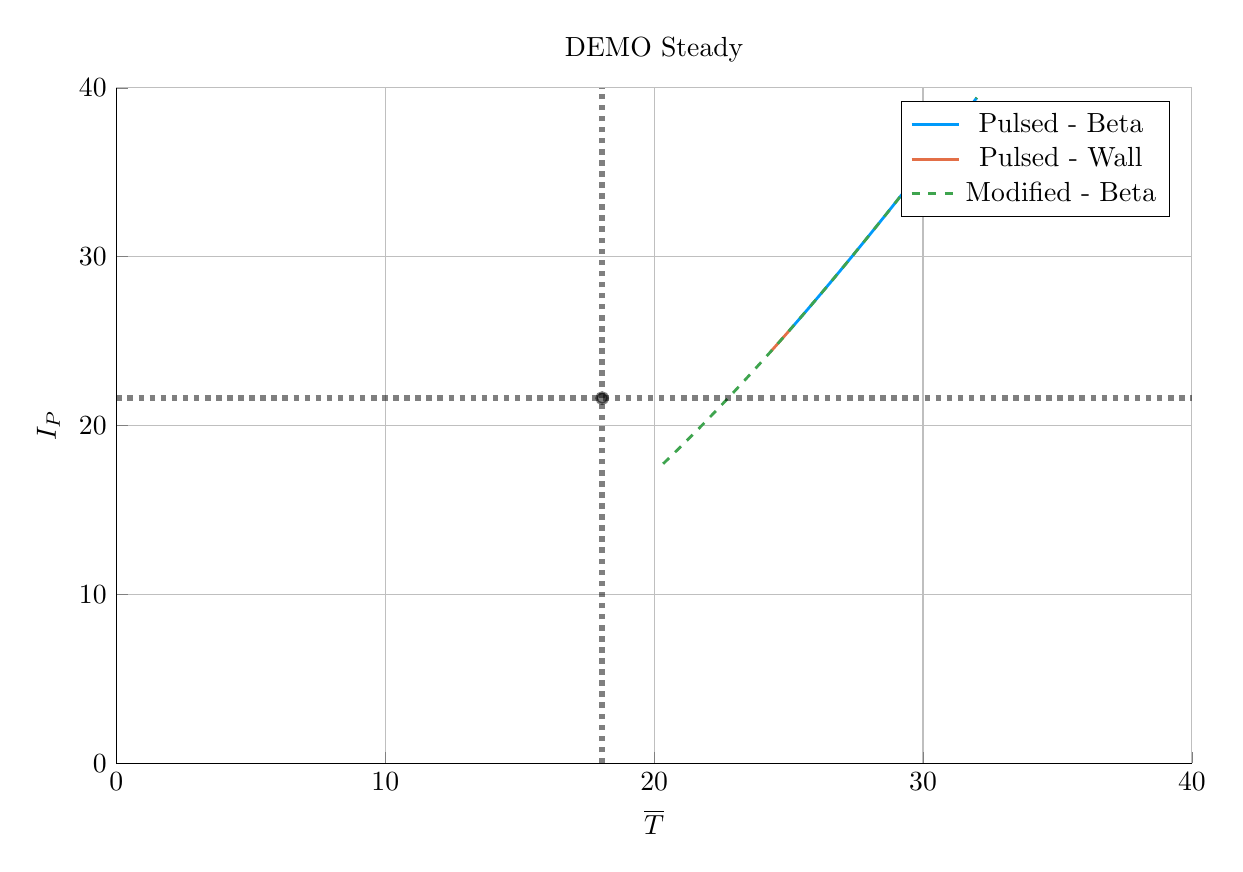
\begin{tikzpicture}[]
\begin{axis}[height = {101.6mm}, ylabel = {${I}_{P}$}, title = {DEMO Steady}, xmin = {0.0}, xmax = {40.0}, ymax = {40.0}, xlabel = {$\overline {T}$}, {unbounded coords=jump, scaled x ticks = false, xticklabel style={rotate = 0}, xmajorgrids = true, xtick = {0.0,10.0,20.0,30.0,40.0}, xticklabels = {0,10,20,30,40}, xtick align = inside, axis lines* = left, scaled y ticks = false, yticklabel style={rotate = 0}, ymajorgrids = true, ytick = {0.0,10.0,20.0,30.0,40.0}, yticklabels = {0,10,20,30,40}, ytick align = inside, axis lines* = left,     xshift = 0.0mm,
    yshift = 0.0mm,
    axis background/.style={fill={rgb,1:red,1.00000000;green,1.00000000;blue,1.00000000}}
, colorbar style={title=}}, ymin = {0.0}, width = {152.4mm}]\addplot+ [color = {rgb,1:red,0.00000000;green,0.60560316;blue,0.97868012},
draw opacity=1.0,
line width=1,
solid,mark = none,
mark size = 2.0,
mark options = {
    color = {rgb,1:red,0.00000000;green,0.00000000;blue,0.00000000}, draw opacity = 1.0,
    fill = {rgb,1:red,0.00000000;green,0.60560316;blue,0.97868012}, fill opacity = 1.0,
    line width = 1,
    rotate = 0,
    solid
}]coordinates {
(25.053735982163357, 25.677558860299992)
(25.333333333333332, 26.189593064380034)
(25.666666666666668, 26.80548085953921)
(26.0, 27.427148406840605)
(26.333333333333332, 28.054440831282633)
(26.666666666666668, 28.68719962041386)
(27.0, 29.325262818659787)
(27.333333333333332, 29.968465226287904)
(27.666666666666668, 30.6166386025962)
(28.0, 31.269611872884024)
(28.333333333333332, 31.92721133872904)
(28.666666666666668, 32.589260891064264)
(29.0, 33.25558222552837)
(29.333333333333332, 33.925995059549685)
(29.666666666666668, 34.60031735061725)
(30.0, 35.27836551518855)
(30.333333333333332, 35.95995464768734)
(30.666666666666668, 36.644898739049395)
(31.0, 37.333010894283476)
(31.333333333333332, 38.02410354852819)
(31.666666666666668, 38.717988681099214)
(32.0, 39.41447802704077)
};
\addlegendentry{Pulsed - Beta}
\addplot+ [color = {rgb,1:red,0.88887350;green,0.43564919;blue,0.27812294},
draw opacity=1.0,
line width=1,
solid,mark = none,
mark size = 2.0,
mark options = {
    color = {rgb,1:red,0.00000000;green,0.00000000;blue,0.00000000}, draw opacity = 1.0,
    fill = {rgb,1:red,0.88887350;green,0.43564919;blue,0.27812294}, fill opacity = 1.0,
    line width = 1,
    rotate = 0,
    solid
}]coordinates {
(24.333333333333332, 24.378107374495485)
(24.666666666666668, 24.975762903314084)
(25.0, 25.579637086786484)
(25.053735982163357, 25.677558860299992)
};
\addlegendentry{Pulsed - Wall}
\addplot+ [color = {rgb,1:red,0.24222430;green,0.64327509;blue,0.30444865},
draw opacity=1.0,
line width=1,
dashed,mark = none,
mark size = 2.0,
mark options = {
    color = {rgb,1:red,0.00000000;green,0.00000000;blue,0.00000000}, draw opacity = 1.0,
    fill = {rgb,1:red,0.24222430;green,0.64327509;blue,0.30444865}, fill opacity = 1.0,
    line width = 1,
    rotate = 0,
    solid
}]coordinates {
(20.333333333333332, 17.737142606162497)
(20.666666666666668, 18.250736761644205)
(21.0, 18.771889258341997)
(21.333333333333332, 19.300518519223587)
(21.666666666666668, 19.836537357082282)
(22.0, 20.37985305559639)
(22.333333333333332, 20.930367463801495)
(22.666666666666668, 21.487977099646507)
(23.0, 22.05257326267931)
(23.333333333333332, 22.62404215595106)
(23.666666666666668, 23.202265017123075)
(24.0, 23.787118258664318)
(24.333333333333332, 24.378473616949)
(24.666666666666668, 24.976198309995638)
(25.0, 25.58015520352756)
(25.333333333333332, 26.19020298497985)
(25.666666666666668, 26.806196345025047)
(26.0, 27.427986166140983)
(26.333333333333332, 28.055419717698932)
(26.666666666666668, 28.688340857006587)
(27.0, 29.3265902357016)
(27.333333333333332, 29.970005510854897)
(27.666666666666668, 30.61842156011136)
(28.0, 31.27167070016686)
(28.333333333333332, 31.92958290785876)
(28.666666666666668, 32.591986043126525)
(29.0, 33.25870607308836)
(29.333333333333332, 33.929567296470175)
(29.666666666666668, 34.604392567622554)
(30.0, 35.28300351936469)
(30.333333333333332, 35.96522078390488)
(30.666666666666668, 36.650864211102025)
(31.0, 37.3397530833557)
(31.333333333333332, 38.03170632643894)
(31.666666666666668, 38.726542715621264)
(32.0, 39.424081076468326)
};
\addlegendentry{Modified - Beta}
\addplot+ [color = {rgb,1:red,0.00000000;green,0.00000000;blue,0.00000000},
draw opacity=0.5,
line width=2,
dotted,mark = none,
mark size = 2.0,
mark options = {
    color = {rgb,1:red,0.00000000;green,0.00000000;blue,0.00000000}, draw opacity = 0.5,
    fill = {rgb,1:red,0.00000000;green,0.00000000;blue,0.00000000}, fill opacity = 0.5,
    line width = 1,
    rotate = 0,
    solid
},forget plot]coordinates {
(0.0, 21.627)
(40.0, 21.627)
};
\addplot+ [color = {rgb,1:red,0.00000000;green,0.00000000;blue,0.00000000},
draw opacity=0.5,
line width=2,
dotted,mark = none,
mark size = 2.0,
mark options = {
    color = {rgb,1:red,0.00000000;green,0.00000000;blue,0.00000000}, draw opacity = 0.5,
    fill = {rgb,1:red,0.00000000;green,0.00000000;blue,0.00000000}, fill opacity = 0.5,
    line width = 1,
    rotate = 0,
    solid
},forget plot]coordinates {
(18.067, 0.0)
(18.067, 40.0)
};
\addplot+[draw=none, color = {rgb,1:red,0.00000000;green,0.00000000;blue,0.00000000},
draw opacity=0.5,
line width=0,
solid,mark = *,
mark size = 2.0,
mark options = {
    color = {rgb,1:red,0.00000000;green,0.00000000;blue,0.00000000}, draw opacity = 0.5,
    fill = {rgb,1:red,0.00000000;green,0.00000000;blue,0.00000000}, fill opacity = 0.5,
    line width = 1,
    rotate = 0,
    solid
},forget plot] coordinates {
(18.067, 21.627)
};
\end{axis}

\end{tikzpicture}

    \end{adjustbox}
        \caption{$I_P$ vs $\overline T$}
    \end{subfigure}
    \hfill \hfill ~\\ ~\\ ~\\
    \caption{Demo Steady Model Comparison} ~\\
\end{figure*}

\begin{table}[h!]
\centering  
\caption{Demo Steady Variables}
\hfill
\begin{subtable}[t]{0.4\textwidth}
\centering  
\caption{Input Variables} ~\\
\begin{tabular}{ c|c } 

Input            & Value           \\
\hline
$H$              & 1.4             \\
$Q$              & 24.46           \\
$N_{G}$          & 1.2             \\
$\epsilon$       & 0.385           \\
$\kappa_{95}$    & 1.8             \\
$\delta_{95}$    & 0.333           \\
$\nu_{n}$        & 0.3972          \\
$\nu_{T}$        & 0.9187          \\
$l_{i}$          & 0.9             \\
$A$              & 2.856           \\
$Z_{eff}$        & 4.708           \\
$f_{D}$          & 0.7366          \\
$\tau_{FT}$      & 1.6e9           \\
$B_{CS}$         & 12.85           \\

\end{tabular}
\end{subtable}
\hfill
\begin{subtable}[t]{0.5\textwidth}
\centering  
\caption{Output Variables} ~\\
\begin{tabular}{ c|c|c } 

Output           & Original         & Fussy.jl        \\  
\hline
$R_{0}$          & 7.5              & 8.2           \\
$B_{0}$          & 5.627            & 6.307           \\
$I_{P}$          & 21.63            & 30.93           \\
$\overline n$    & 0.8746           & 1.048           \\
$\overline T$    & 18.07            & 27.83           \\
$\beta_{N}$       & 0.038            & -           \\
$q_{95}$         & 4.405            & 3.761           \\
$P_{W}$          & 1.911            & 4.151           \\
$f_{BS}$         & 0.611            & 0.424          \\
$f_{CD}$         & 0.389            & 0.576          \\
$f_{ID}$         & -              & -             \\
$\volume$         & 2217           & 2879          \\
$P_{F}$          & 3255           & 8971          \\
$\eta_{CD}$      & 0.4152           & -          \\

\end{tabular}
\end{subtable}
\hfill
\hfill
\end{table}

\newpage 

\subsubsection{DEMO Pulsed -- A Pulsed ITER Successor}

This pulsed version of DEMO is the only reactor in our collection that is not run in steady-state. As such, it may be the most important one. The first thing that is abundantly clear is that this design actually has no valid wall loading portion -- only a kink and beta curve exist! Even so, the results match pretty well. It should be noted, though, that this current drive is treated as an input and not solved self-consistently.

\begin{figure*}[h!]
    \centering
    \hfill 
    \begin{subfigure}[t]{0.45\textwidth}
        \centering
    \begin{adjustbox}{width=\textwidth}
      \Large
      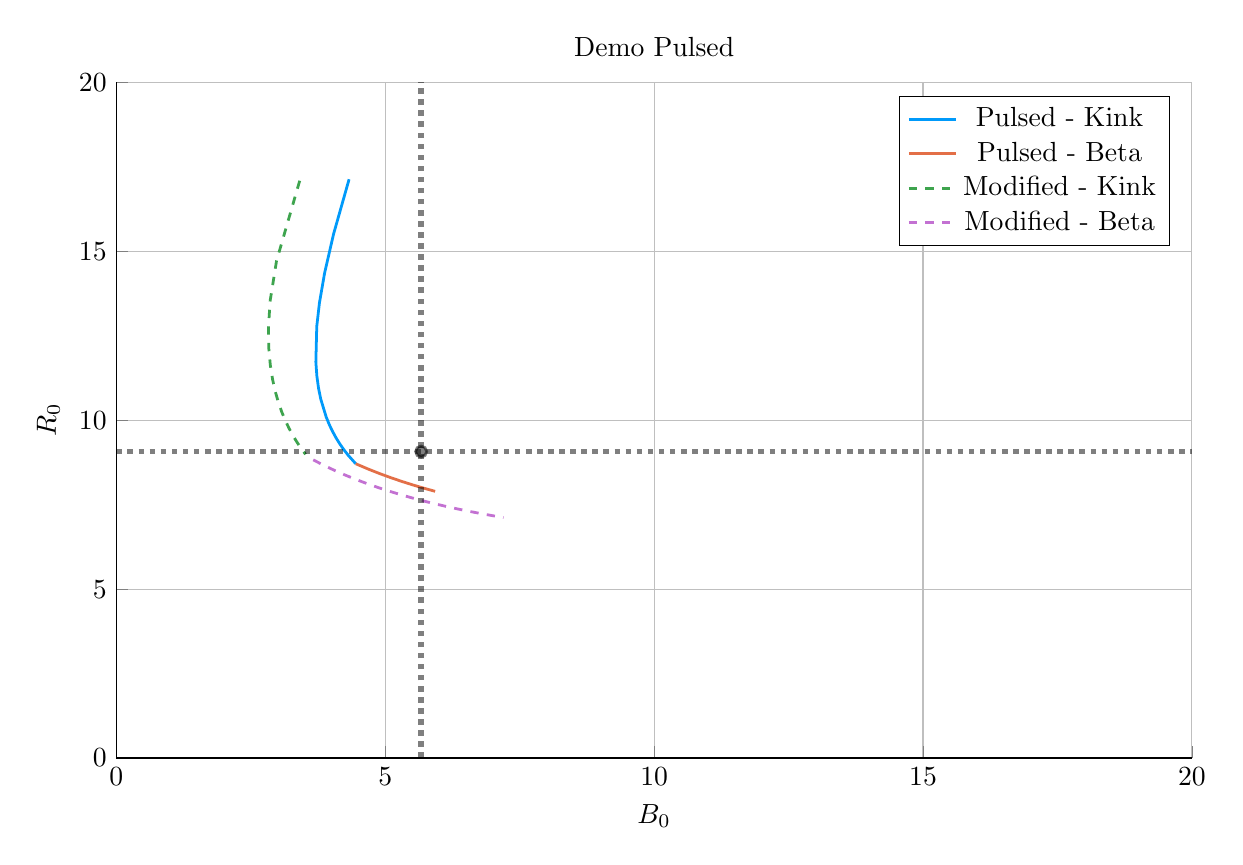
\begin{tikzpicture}[]
\begin{axis}[height = {101.6mm}, ylabel = {${R}_{0}$}, title = {Demo Pulsed}, xmin = {0.0}, xmax = {20.0}, ymax = {20.0}, xlabel = {${B}_{0}$}, {unbounded coords=jump, scaled x ticks = false, xticklabel style={rotate = 0}, xmajorgrids = true, xtick = {0.0,5.0,10.0,15.0,20.0}, xticklabels = {0,5,10,15,20}, xtick align = inside, axis lines* = left, scaled y ticks = false, yticklabel style={rotate = 0}, ymajorgrids = true, ytick = {0.0,5.0,10.0,15.0,20.0}, yticklabels = {0,5,10,15,20}, ytick align = inside, axis lines* = left,     xshift = 0.0mm,
    yshift = 0.0mm,
    axis background/.style={fill={rgb,1:red,1.00000000;green,1.00000000;blue,1.00000000}}
, colorbar style={title=}}, ymin = {0.0}, width = {152.4mm}]\addplot+ [color = {rgb,1:red,0.00000000;green,0.60560316;blue,0.97868012},
draw opacity=1.0,
line width=1,
solid,mark = none,
mark size = 2.0,
mark options = {
    color = {rgb,1:red,0.00000000;green,0.00000000;blue,0.00000000}, draw opacity = 1.0,
    fill = {rgb,1:red,0.00000000;green,0.60560316;blue,0.97868012}, fill opacity = 1.0,
    line width = 1,
    rotate = 0,
    solid
}]coordinates {
(4.327031075670194, 17.134796748649162)
(4.038214026054326, 15.511755022601415)
(3.8713719163129245, 14.355562963913712)
(3.7758613845615545, 13.476675762289453)
(3.7257856761317214, 12.778294295391971)
(3.7090473695925437, 11.723065749829066)
(3.727711597554826, 11.30970201784727)
(3.7586131667481433, 10.94971275897184)
(3.799052518631718, 10.632190690377048)
(3.901290136389271, 10.09455415135144)
(3.960577465316514, 9.863813619410237)
(4.0241209645210345, 9.653307397969705)
(4.0912717805663785, 9.460162902699798)
(4.161514602943343, 9.28206292757184)
(4.2344343960723005, 9.117114543572253)
(4.309692554546368, 8.963753917462126)
(4.450417240491067, 8.712493965092264)
};
\addlegendentry{Pulsed - Kink}
\addplot+ [color = {rgb,1:red,0.88887350;green,0.43564919;blue,0.27812294},
draw opacity=1.0,
line width=1,
solid,mark = none,
mark size = 2.0,
mark options = {
    color = {rgb,1:red,0.00000000;green,0.00000000;blue,0.00000000}, draw opacity = 1.0,
    fill = {rgb,1:red,0.88887350;green,0.43564919;blue,0.27812294}, fill opacity = 1.0,
    line width = 1,
    rotate = 0,
    solid
}]coordinates {
(4.450417240491067, 8.712493965092264)
(4.490148631384312, 8.684308742646298)
(4.692490181445514, 8.547262773806349)
(4.8960344619053355, 8.41947837460442)
(5.100651132702229, 8.30014929484307)
(5.306202822090688, 8.188581738801314)
(5.512545696627038, 8.084175191078112)
(5.719530043226767, 7.986407002697611)
(5.927000883375481, 7.894819882619234)
};
\addlegendentry{Pulsed - Beta}
\addplot+ [color = {rgb,1:red,0.24222430;green,0.64327509;blue,0.30444865},
draw opacity=1.0,
line width=1,
dashed,mark = none,
mark size = 2.0,
mark options = {
    color = {rgb,1:red,0.00000000;green,0.00000000;blue,0.00000000}, draw opacity = 1.0,
    fill = {rgb,1:red,0.24222430;green,0.64327509;blue,0.30444865}, fill opacity = 1.0,
    line width = 1,
    rotate = 0,
    solid
}]coordinates {
(3.4087424183072135, 17.090884129081292)
(2.977074181068944, 14.713048632784332)
(2.8592500074202523, 13.541171522519205)
(2.827199220063259, 12.740024138753894)
(2.8339789008667826, 12.12574468151967)
(2.862412302880871, 11.626187613249266)
(2.9044598258085443, 11.205091848948229)
(2.95577893007882, 10.841432203317366)
(3.0137895352525907, 10.521822649209419)
(3.076849710218805, 10.23716073884787)
(3.1438583711612704, 9.980947801083442)
(3.214045733980633, 9.748367275345563)
(3.2868548955983727, 9.535742205343247)
(3.361871149981842, 9.340197658526863)
(3.4387778750377818, 9.15944098345979)
(3.5173279629378453, 8.991613349767409)
};
\addlegendentry{Modified - Kink}
\addplot+ [color = {rgb,1:red,0.76444018;green,0.44411178;blue,0.82429754},
draw opacity=1.0,
line width=1,
dashed,mark = none,
mark size = 2.0,
mark options = {
    color = {rgb,1:red,0.00000000;green,0.00000000;blue,0.00000000}, draw opacity = 1.0,
    fill = {rgb,1:red,0.76444018;green,0.44411178;blue,0.82429754}, fill opacity = 1.0,
    line width = 1,
    rotate = 0,
    solid
}]coordinates {
(3.6607028750648505, 8.825949645171955)
(3.8574448036470477, 8.664618827122876)
(4.056375867871351, 8.51434867582932)
(4.257366397480293, 8.374075613831488)
(4.460279103534801, 8.242896218794312)
(4.664969389370631, 8.12003771613466)
(4.871285596007394, 8.004834914067093)
(5.07906923307514, 7.896711937521184)
(5.288155233306219, 7.795167587687744)
(5.498372259673351, 7.699763475973523)
(5.709543087166185, 7.610114306522102)
(5.921485076209294, 7.525879840414137)
(6.134010749367255, 7.446758190646709)
(6.346928478632384, 7.372480180910637)
(6.560043285872518, 7.302804563889649)
(6.773157754368795, 7.237513941672651)
(6.986073044284746, 7.176411266758267)
(7.198590001107076, 7.119316828230052)
};
\addlegendentry{Modified - Beta}
\addplot+ [color = {rgb,1:red,0.00000000;green,0.00000000;blue,0.00000000},
draw opacity=0.5,
line width=2,
dotted,mark = none,
mark size = 2.0,
mark options = {
    color = {rgb,1:red,0.00000000;green,0.00000000;blue,0.00000000}, draw opacity = 0.5,
    fill = {rgb,1:red,0.00000000;green,0.00000000;blue,0.00000000}, fill opacity = 0.5,
    line width = 1,
    rotate = 0,
    solid
},forget plot]coordinates {
(0.0, 9.072)
(20.0, 9.072)
};
\addplot+ [color = {rgb,1:red,0.00000000;green,0.00000000;blue,0.00000000},
draw opacity=0.5,
line width=2,
dotted,mark = none,
mark size = 2.0,
mark options = {
    color = {rgb,1:red,0.00000000;green,0.00000000;blue,0.00000000}, draw opacity = 0.5,
    fill = {rgb,1:red,0.00000000;green,0.00000000;blue,0.00000000}, fill opacity = 0.5,
    line width = 1,
    rotate = 0,
    solid
},forget plot]coordinates {
(5.667, 0.0)
(5.667, 20.0)
};
\addplot+[draw=none, color = {rgb,1:red,0.00000000;green,0.00000000;blue,0.00000000},
draw opacity=0.5,
line width=0,
solid,mark = *,
mark size = 2.0,
mark options = {
    color = {rgb,1:red,0.00000000;green,0.00000000;blue,0.00000000}, draw opacity = 0.5,
    fill = {rgb,1:red,0.00000000;green,0.00000000;blue,0.00000000}, fill opacity = 0.5,
    line width = 1,
    rotate = 0,
    solid
},forget plot] coordinates {
(5.667, 9.072)
};
\end{axis}

\end{tikzpicture}

    \end{adjustbox}
        \caption{$R_0$ vs $B_0$}
    \end{subfigure}
    \hfill
    \begin{subfigure}[t]{0.45\textwidth}
        \centering
    \begin{adjustbox}{width=\textwidth}
      \Large
      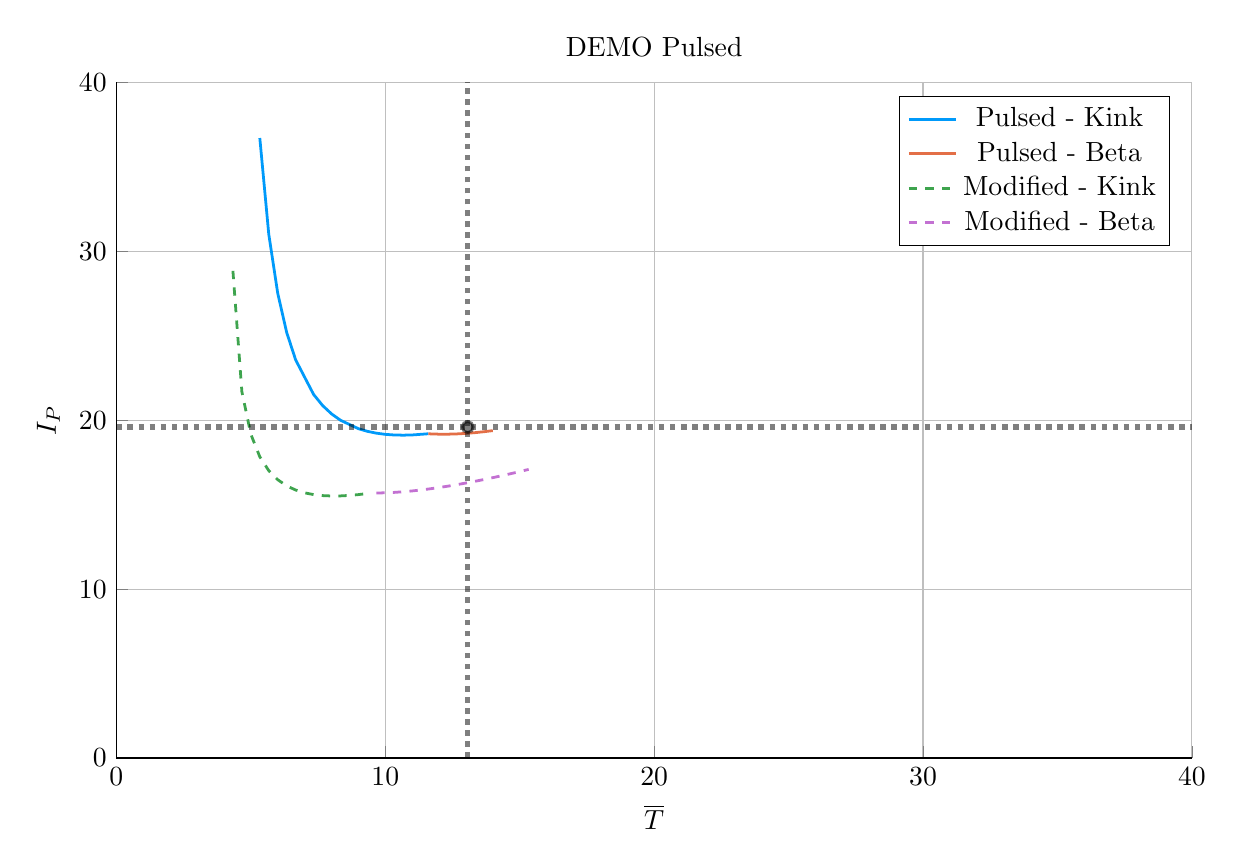
\begin{tikzpicture}[]
\begin{axis}[height = {101.6mm}, ylabel = {${I}_{P}$}, title = {DEMO Pulsed}, xmin = {0.0}, xmax = {40.0}, ymax = {40.0}, xlabel = {$\overline {T}$}, {unbounded coords=jump, scaled x ticks = false, xticklabel style={rotate = 0}, xmajorgrids = true, xtick = {0.0,10.0,20.0,30.0,40.0}, xticklabels = {0,10,20,30,40}, xtick align = inside, axis lines* = left, scaled y ticks = false, yticklabel style={rotate = 0}, ymajorgrids = true, ytick = {0.0,10.0,20.0,30.0,40.0}, yticklabels = {0,10,20,30,40}, ytick align = inside, axis lines* = left,     xshift = 0.0mm,
    yshift = 0.0mm,
    axis background/.style={fill={rgb,1:red,1.00000000;green,1.00000000;blue,1.00000000}}
, colorbar style={title=}}, ymin = {0.0}, width = {152.4mm}]\addplot+ [color = {rgb,1:red,0.00000000;green,0.60560316;blue,0.97868012},
draw opacity=1.0,
line width=1,
solid,mark = none,
mark size = 2.0,
mark options = {
    color = {rgb,1:red,0.00000000;green,0.00000000;blue,0.00000000}, draw opacity = 1.0,
    fill = {rgb,1:red,0.00000000;green,0.60560316;blue,0.97868012}, fill opacity = 1.0,
    line width = 1,
    rotate = 0,
    solid
}]coordinates {
(5.333333333333333, 36.71051032912112)
(5.666666666666667, 31.014995367356207)
(6.0, 27.51734786322149)
(6.333333333333333, 25.19534286389616)
(6.666666666666667, 23.57285610926683)
(7.333333333333333, 21.52905816503197)
(7.666666666666667, 20.874444053021588)
(8.0, 20.377542510464334)
(8.333333333333334, 19.99951688957442)
(9.0, 19.499202175706746)
(9.333333333333334, 19.343044014643887)
(9.666666666666666, 19.233955791269285)
(10.0, 19.16365729524907)
(10.333333333333334, 19.125701869840853)
(10.666666666666666, 19.11499858904485)
(11.0, 19.127475979338943)
(11.600962879632572, 19.198383823705257)
};
\addlegendentry{Pulsed - Kink}
\addplot+ [color = {rgb,1:red,0.88887350;green,0.43564919;blue,0.27812294},
draw opacity=1.0,
line width=1,
solid,mark = none,
mark size = 2.0,
mark options = {
    color = {rgb,1:red,0.00000000;green,0.00000000;blue,0.00000000}, draw opacity = 1.0,
    fill = {rgb,1:red,0.88887350;green,0.43564919;blue,0.27812294}, fill opacity = 1.0,
    line width = 1,
    rotate = 0,
    solid
}]coordinates {
(11.600962879632572, 19.198383823705257)
(11.666666666666666, 19.192414153878335)
(12.0, 19.174087186739918)
(12.333333333333334, 19.17397121853779)
(12.666666666666666, 19.189978018951553)
(13.0, 19.220357277326283)
(13.333333333333334, 19.263633100211838)
(13.666666666666666, 19.31855421750887)
(14.0, 19.384054548489104)
};
\addlegendentry{Pulsed - Beta}
\addplot+ [color = {rgb,1:red,0.24222430;green,0.64327509;blue,0.30444865},
draw opacity=1.0,
line width=1,
dashed,mark = none,
mark size = 2.0,
mark options = {
    color = {rgb,1:red,0.00000000;green,0.00000000;blue,0.00000000}, draw opacity = 1.0,
    fill = {rgb,1:red,0.24222430;green,0.64327509;blue,0.30444865}, fill opacity = 1.0,
    line width = 1,
    rotate = 0,
    solid
}]coordinates {
(4.333333333333333, 28.845639077165217)
(4.666666666666667, 21.687713986294685)
(5.0, 19.170340224057398)
(5.333333333333333, 17.83397336320386)
(5.666666666666667, 17.01478565989059)
(6.0, 16.477486603636205)
(6.333333333333333, 16.113958654578386)
(6.666666666666667, 15.866460603971907)
(7.0, 15.700928946757587)
(7.333333333333333, 15.59578560596909)
(7.666666666666667, 15.536607983152381)
(8.0, 15.513342675582972)
(8.333333333333334, 15.518740955012225)
(8.666666666666666, 15.547428978968492)
(9.0, 15.595329068459918)
(9.333333333333334, 15.659285368310089)
};
\addlegendentry{Modified - Kink}
\addplot+ [color = {rgb,1:red,0.76444018;green,0.44411178;blue,0.82429754},
draw opacity=1.0,
line width=1,
dashed,mark = none,
mark size = 2.0,
mark options = {
    color = {rgb,1:red,0.00000000;green,0.00000000;blue,0.00000000}, draw opacity = 1.0,
    fill = {rgb,1:red,0.76444018;green,0.44411178;blue,0.82429754}, fill opacity = 1.0,
    line width = 1,
    rotate = 0,
    solid
}]coordinates {
(9.666666666666666, 15.691192911261952)
(10.0, 15.70165788278533)
(10.333333333333334, 15.726578234093749)
(10.666666666666666, 15.764127054896537)
(11.0, 15.812802650736373)
(11.333333333333334, 15.871360766004056)
(11.666666666666666, 15.938763317563621)
(12.0, 16.014139065408)
(12.333333333333334, 16.09675304572932)
(12.666666666666666, 16.185982524147033)
(13.0, 16.281297862810217)
(13.333333333333334, 16.382247130746602)
(13.666666666666666, 16.488443597982137)
(14.0, 16.5995554722192)
(14.333333333333334, 16.715297396529092)
(14.666666666666666, 16.83542334285969)
(15.0, 16.959720624053933)
(15.333333333333334, 17.088004807739882)
};
\addlegendentry{Modified - Beta}
\addplot+ [color = {rgb,1:red,0.00000000;green,0.00000000;blue,0.00000000},
draw opacity=0.5,
line width=2,
dotted,mark = none,
mark size = 2.0,
mark options = {
    color = {rgb,1:red,0.00000000;green,0.00000000;blue,0.00000000}, draw opacity = 0.5,
    fill = {rgb,1:red,0.00000000;green,0.00000000;blue,0.00000000}, fill opacity = 0.5,
    line width = 1,
    rotate = 0,
    solid
},forget plot]coordinates {
(0.0, 19.6)
(40.0, 19.6)
};
\addplot+ [color = {rgb,1:red,0.00000000;green,0.00000000;blue,0.00000000},
draw opacity=0.5,
line width=2,
dotted,mark = none,
mark size = 2.0,
mark options = {
    color = {rgb,1:red,0.00000000;green,0.00000000;blue,0.00000000}, draw opacity = 0.5,
    fill = {rgb,1:red,0.00000000;green,0.00000000;blue,0.00000000}, fill opacity = 0.5,
    line width = 1,
    rotate = 0,
    solid
},forget plot]coordinates {
(13.065, 0.0)
(13.065, 40.0)
};
\addplot+[draw=none, color = {rgb,1:red,0.00000000;green,0.00000000;blue,0.00000000},
draw opacity=0.5,
line width=0,
solid,mark = *,
mark size = 2.0,
mark options = {
    color = {rgb,1:red,0.00000000;green,0.00000000;blue,0.00000000}, draw opacity = 0.5,
    fill = {rgb,1:red,0.00000000;green,0.00000000;blue,0.00000000}, fill opacity = 0.5,
    line width = 1,
    rotate = 0,
    solid
},forget plot] coordinates {
(13.065, 19.6)
};
\end{axis}

\end{tikzpicture}

    \end{adjustbox}
        \caption{$I_P$ vs $\overline T$}
    \end{subfigure}
    \hfill \hfill ~\\ ~\\ ~\\
    \caption{Demo Pulsed Model Comparison} ~\\
\end{figure*}

\begin{table}[h!]
\centering  
\caption{Demo Pulsed Variables}
\hfill
\begin{subtable}[t]{0.4\textwidth}
\centering  
\caption{Input Variables} ~\\
\begin{tabular}{ c|c } 

Input            & Value           \\
\hline
$H$              & 1.1             \\
$Q$              & 39.86           \\
$N_{G}$          & 1.2             \\
$\epsilon$       & 0.3226          \\
$\kappa_{95}$    & 1.59            \\
$\delta_{95}$    & 0.333           \\
$\nu_{n}$        & 0.27            \\
$\nu_{T}$        & 1.094           \\
$l_{i}$          & 1.155           \\
$A$              & 2.735           \\
$Z_{eff}$        & 2.584           \\
$f_{D}$          & 0.7753          \\
$\tau_{FT}$      & 7273          \\
$B_{CS}$         & 12.77           \\

\end{tabular}
\end{subtable}
\hfill
\begin{subtable}[t]{0.5\textwidth}
\centering  
\caption{Output Variables} ~\\
\begin{tabular}{ c|c|c } 

Output           & Original         & Fussy.jl        \\
\hline
$R_{0}$          & 9.07            & 8.10             \\
$B_{0}$          & 5.67            & 5.48            \\
$I_{P}$          & 19.6             & 19.3           \\
$\overline n$    & 0.7983           & 0.9795          \\
$\overline T$    & 13.06            & 13.28           \\
$\beta_{N}$       & 0.0259           & -          \\
$q_{95}$         & 3.247            & 2.853           \\
$P_{W}$          & 1.05             & 1.47           \\
$f_{BS}$         & 0.348            & 0.164          \\
$f_{CD}$         & 0.096            & 0.106          \\
$f_{ID}$         & 0.557            & 0.730          \\
$\volume$         & 2502           & 1751          \\
$P_{F}$          & 2037           & 2376          \\
$\eta_{CD}$      & 0.2721           & -     

\end{tabular}
\end{subtable}
\hfill
\hfill
\end{table}

\section{Developing Prototype Reactors}

Now that the model used in Fussy.jl has been tested against other fusion systems codes in the field, we will develop our own prototype reactors. Because this paper is about making a levelized comparison of pulsed and steady-state tokamaks, we will develop middle-of-the-road reactors that only differ by operating mode. 

The steady-state prototype, Charybdis, is the obvious choice to start with -- as the model was tested against four of these typed reactors. It was also pointed out that the model did remarkably well when recreating ARC. As the authors share many of the ARC team's philosophies, Charybdis uses \replaced{static}{fixed} parameters very similar to them.

Next, although led to believe Charybdis' pulsed twin reactor -- Proteus -- would be created by a simple flip of the switch, it was a slight oversimplification. The first difference is that the pulsed twin, Proteus, is assumed to be purely pulsed: $\eta_{CD} = 0$. Further, the bootstrap current is much less important than it was for steady-state tokamaks. This corresponds to a current profile peaked at the origin -- i.e. a parabola. Numerically, this is done by raising $l_i$ from around 5.5 to 6.

The final difference creates the largest change in the twin reactors: the choice of miracle. As hinted several times before, the H factor is a common way designers artificially boost the confinement of their machines. This H value will thus be the miracle for Charybdis, the steady-state prototype. Next, as the main conclusion of this paper is to state the advantages of high magnetic field, a free way to boost a central solenoid -- through $B_{CS}$ -- will be employed using HTS coils.

Opposite the order of how they were designed, the goal now is to lock down a value of $B_{CS}$ for Proteus and then use it to set the H factor for Charybdis. This selection algorithm is depicted in \cref{fig:selection}. For Proteus, the point locked down was $B_{CS} = 20 \ \textnormal{T}$, which occurred at a fusion power ($P_F$) of around 1250 MW. As shown in the cost curve, this was at a point where the ratio between the minimum capital cost and the minimum cost-per-watt saturated. This choice of a 1250 MW reactor then led to Charybdis having an H factor of 1.7.

\begin{figure}[h!]
\centering
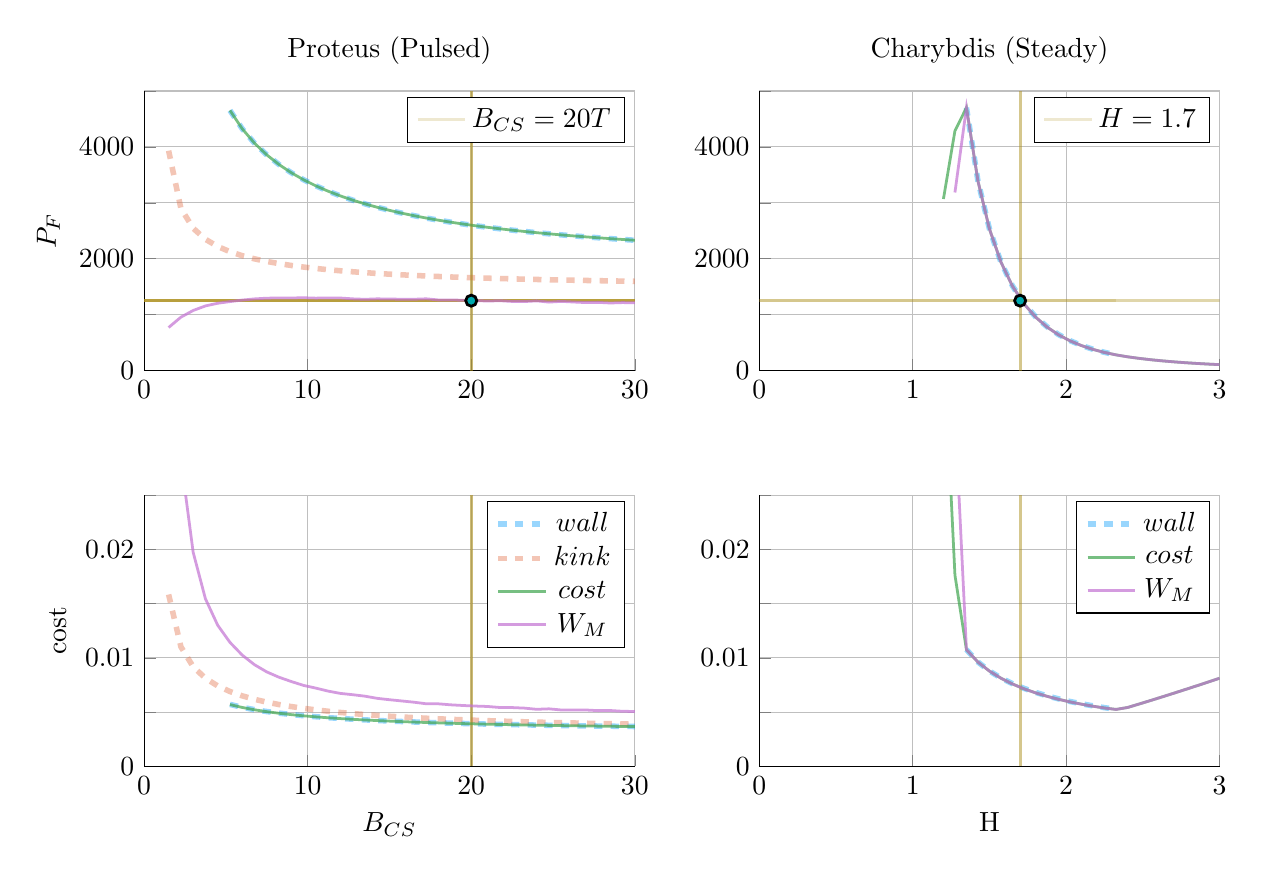
\begin{tikzpicture}[]
\begin{axis}[height = {51.32916666666667mm}, ylabel = {$P_F$}, title = {Proteus (Pulsed)}, xmin = {0}, xmax = {30.0}, ymax = {5000.0}, xlabel = {}, {unbounded coords=jump, scaled x ticks = false, xticklabel style={rotate = 0}, xmajorgrids = true, xtick = {0.0,10.0,20.0,30.0}, xticklabels = {0,10,20,30}, xtick align = inside, axis lines* = left, scaled y ticks = false, yticklabel style={rotate = 0}, ymajorgrids = true, ytick = {0,1000,2000,3000,4000,5000}, yticklabels = {0,,2000,,4000,}, ytick align = inside, axis lines* = left,     xshift = 0.0mm,
    yshift = 50.27mm,
    axis background/.style={fill={rgb,1:red,1.00000000;green,1.00000000;blue,1.00000000}}
}, ymin = {2.220446049250313e-16}, width = {78.14027777777778mm}]\addplot+ [color = {rgb,1:red,0.67554396;green,0.55566233;blue,0.09423434},
draw opacity=0.2,
line width=1,
solid,mark = none,
mark size = 2.0,
mark options = {
    color = {rgb,1:red,0.00000000;green,0.00000000;blue,0.00000000}, draw opacity = 1.0,
    fill = {rgb,1:red,0.67554396;green,0.55566233;blue,0.09423434}, fill opacity = 1.0,
    line width = 1,
    rotate = 0,
    solid
}]coordinates {
(20.0, 2.220446049250313e-16)
(20.0, 5000.0)
};
\addlegendentry{$B_{CS} = 20 T$}
\addplot+ [color = {rgb,1:red,0.67554396;green,0.55566233;blue,0.09423434},
draw opacity=0.2,
line width=1,
solid,mark = none,
mark size = 2.0,
mark options = {
    color = {rgb,1:red,0.00000000;green,0.00000000;blue,0.00000000}, draw opacity = 1.0,
    fill = {rgb,1:red,0.67554396;green,0.55566233;blue,0.09423434}, fill opacity = 1.0,
    line width = 1,
    rotate = 0,
    solid
},forget plot]coordinates {
(0.0, 1250.0)
(30.0, 1250.0)
};
\addplot+[draw=none, color = {rgb,1:red,0.00000048;green,0.66575898;blue,0.68099695},
draw opacity=1.0,
line width=0,
solid,mark = *,
mark size = 2.0,
mark options = {
    color = {rgb,1:red,0.00000000;green,0.00000000;blue,0.00000000}, draw opacity = 1.0,
    fill = {rgb,1:red,0.00000048;green,0.66575898;blue,0.68099695}, fill opacity = 1.0,
    line width = 1,
    rotate = 0,
    solid
},forget plot] coordinates {
(20, 1250)
};
\addplot+ [color = {rgb,1:red,0.67554396;green,0.55566233;blue,0.09423434},
draw opacity=0.2,
line width=1,
solid,mark = none,
mark size = 2.0,
mark options = {
    color = {rgb,1:red,0.00000000;green,0.00000000;blue,0.00000000}, draw opacity = 1.0,
    fill = {rgb,1:red,0.67554396;green,0.55566233;blue,0.09423434}, fill opacity = 1.0,
    line width = 1,
    rotate = 0,
    solid
},forget plot]coordinates {
(0.0, 1250.0)
(30.0, 1250.0)
};
\addplot+ [color = {rgb,1:red,0.00000000;green,0.60560316;blue,0.97868012},
draw opacity=0.4,
line width=2,
dashed,mark = none,
mark size = 2.0,
mark options = {
    color = {rgb,1:red,0.00000000;green,0.00000000;blue,0.00000000}, draw opacity = 1.0,
    fill = {rgb,1:red,0.00000000;green,0.60560316;blue,0.97868012}, fill opacity = 1.0,
    line width = 1,
    rotate = 0,
    solid
},forget plot]coordinates {
(5.25, 4651.734735476011)
(6.0, 4323.6250098364)
(6.75, 4065.99692078527)
(7.5, 3857.273578687972)
(8.25, 3684.1342593418663)
(9.0, 3537.844669896544)
(9.75, 3412.404653539425)
(10.5, 3303.536032694244)
(11.25, 3208.094051273514)
(12.0, 3123.707522754923)
(12.75, 3048.5495054628623)
(13.5, 2981.185980181023)
(14.25, 2920.472987010462)
(15.0, 2865.484885250518)
(15.75, 2815.463186166668)
(16.5, 2769.7793320244814)
(17.25, 2727.9071420752607)
(18.0, 2689.4020933235493)
(18.75, 2653.885520176901)
(19.5, 2621.0324111911764)
(20.25, 2590.561874678777)
(21.0, 2562.2296107375955)
(21.75, 2535.8219099446264)
(22.5, 2511.150826555893)
(23.25, 2488.050264495335)
(24.0, 2466.372779394113)
(24.75, 2445.986947213969)
(25.5, 2426.775184780072)
(26.25, 2408.6319334297787)
(27.0, 2391.4621364565396)
(27.75, 2375.1799557182867)
(28.5, 2359.707684182671)
(29.25, 2344.974819785335)
(30.0, 2330.917272823136)
};
\addplot+ [color = {rgb,1:red,0.67554396;green,0.55566233;blue,0.09423434},
draw opacity=0.2,
line width=1,
solid,mark = none,
mark size = 2.0,
mark options = {
    color = {rgb,1:red,0.00000000;green,0.00000000;blue,0.00000000}, draw opacity = 1.0,
    fill = {rgb,1:red,0.67554396;green,0.55566233;blue,0.09423434}, fill opacity = 1.0,
    line width = 1,
    rotate = 0,
    solid
},forget plot]coordinates {
(20.0, 2.220446049250313e-16)
(20.0, 5000.0)
};
\addplot+ [color = {rgb,1:red,0.67554396;green,0.55566233;blue,0.09423434},
draw opacity=0.2,
line width=1,
solid,mark = none,
mark size = 2.0,
mark options = {
    color = {rgb,1:red,0.00000000;green,0.00000000;blue,0.00000000}, draw opacity = 1.0,
    fill = {rgb,1:red,0.67554396;green,0.55566233;blue,0.09423434}, fill opacity = 1.0,
    line width = 1,
    rotate = 0,
    solid
},forget plot]coordinates {
(0.0, 1250.0)
(30.0, 1250.0)
};
\addplot+ [color = {rgb,1:red,0.67554396;green,0.55566233;blue,0.09423434},
draw opacity=0.2,
line width=1,
solid,mark = none,
mark size = 2.0,
mark options = {
    color = {rgb,1:red,0.00000000;green,0.00000000;blue,0.00000000}, draw opacity = 1.0,
    fill = {rgb,1:red,0.67554396;green,0.55566233;blue,0.09423434}, fill opacity = 1.0,
    line width = 1,
    rotate = 0,
    solid
},forget plot]coordinates {
(0.0, 1250.0)
(30.0, 1250.0)
};
\addplot+ [color = {rgb,1:red,0.88887350;green,0.43564919;blue,0.27812294},
draw opacity=0.4,
line width=2,
dashed,mark = none,
mark size = 2.0,
mark options = {
    color = {rgb,1:red,0.00000000;green,0.00000000;blue,0.00000000}, draw opacity = 1.0,
    fill = {rgb,1:red,0.88887350;green,0.43564919;blue,0.27812294}, fill opacity = 1.0,
    line width = 1,
    rotate = 0,
    solid
},forget plot]coordinates {
(1.5, 3931.6170696070676)
(2.25, 2900.7235747979908)
(3.0, 2544.8446560898715)
(3.75, 2348.228116500571)
(4.5, 2219.0134794713767)
(5.25, 2125.815532966674)
(6.0, 2054.566085735622)
(6.75, 1997.8824990557177)
(7.5, 1951.4633680592258)
(8.25, 1912.6074536455505)
(9.0, 1879.5196356674505)
(9.75, 1850.953068441656)
(10.5, 1826.0101459658863)
(11.25, 1804.02551415983)
(12.0, 1784.493638745381)
(12.75, 1767.0222758941622)
(13.5, 1751.3015387280175)
(14.25, 1737.0827328069474)
(15.0, 1724.1634044428295)
(15.75, 1712.376890482151)
(16.5, 1701.5841921715175)
(17.25, 1691.6685698179294)
(18.0, 1682.530881991843)
(18.75, 1674.0861755860074)
(19.5, 1666.2615100001372)
(20.25, 1658.9932835127363)
(21.0, 1652.2262595201232)
(21.75, 1645.91179207308)
(22.5, 1640.0070406407558)
(23.25, 1634.4738680952948)
(24.0, 1629.2785569006053)
(24.75, 1624.3908184475338)
(25.5, 1619.7835209277835)
(26.25, 1615.432247074283)
(27.0, 1611.314956936522)
(27.75, 1607.4117026157203)
(28.5, 1603.7043856927105)
(29.25, 1600.1765499289672)
(30.0, 1596.813203261599)
};
\addplot+ [color = {rgb,1:red,0.67554396;green,0.55566233;blue,0.09423434},
draw opacity=0.2,
line width=1,
solid,mark = none,
mark size = 2.0,
mark options = {
    color = {rgb,1:red,0.00000000;green,0.00000000;blue,0.00000000}, draw opacity = 1.0,
    fill = {rgb,1:red,0.67554396;green,0.55566233;blue,0.09423434}, fill opacity = 1.0,
    line width = 1,
    rotate = 0,
    solid
},forget plot]coordinates {
(20.0, 2.220446049250313e-16)
(20.0, 5000.0)
};
\addplot+ [color = {rgb,1:red,0.67554396;green,0.55566233;blue,0.09423434},
draw opacity=0.2,
line width=1,
solid,mark = none,
mark size = 2.0,
mark options = {
    color = {rgb,1:red,0.00000000;green,0.00000000;blue,0.00000000}, draw opacity = 1.0,
    fill = {rgb,1:red,0.67554396;green,0.55566233;blue,0.09423434}, fill opacity = 1.0,
    line width = 1,
    rotate = 0,
    solid
},forget plot]coordinates {
(0.0, 1250.0)
(30.0, 1250.0)
};
\addplot+ [color = {rgb,1:red,0.67554396;green,0.55566233;blue,0.09423434},
draw opacity=0.2,
line width=1,
solid,mark = none,
mark size = 2.0,
mark options = {
    color = {rgb,1:red,0.00000000;green,0.00000000;blue,0.00000000}, draw opacity = 1.0,
    fill = {rgb,1:red,0.67554396;green,0.55566233;blue,0.09423434}, fill opacity = 1.0,
    line width = 1,
    rotate = 0,
    solid
},forget plot]coordinates {
(0.0, 1250.0)
(30.0, 1250.0)
};
\addplot+ [color = {rgb,1:red,0.24222430;green,0.64327509;blue,0.30444865},
draw opacity=0.7,
line width=1,
solid,mark = none,
mark size = 2.0,
mark options = {
    color = {rgb,1:red,0.00000000;green,0.00000000;blue,0.00000000}, draw opacity = 1.0,
    fill = {rgb,1:red,0.24222430;green,0.64327509;blue,0.30444865}, fill opacity = 1.0,
    line width = 1,
    rotate = 0,
    solid
},forget plot]coordinates {
(5.25, 4651.856974626446)
(6.0, 4323.626574700689)
(6.75, 4065.9133365013354)
(7.5, 3857.1264771824617)
(8.25, 3683.9377449687768)
(9.0, 3537.608432111376)
(9.75, 3412.1356303067523)
(10.5, 3303.239361854739)
(11.25, 3207.7736468791713)
(12.0, 3123.3664382128795)
(12.75, 3048.1901722862794)
(13.5, 2980.810371417949)
(14.25, 2920.082728006143)
(15.0, 2865.081335141082)
(15.75, 2815.0474968726217)
(16.5, 2769.352491750233)
(17.25, 2727.4700069605415)
(18.0, 2688.955412764386)
(18.75, 2653.4299583736)
(19.5, 2620.5685580410595)
(20.25, 2590.0902617025704)
(21.0, 2561.7507209540713)
(21.75, 2535.3361812985195)
(22.5, 2510.65866319561)
(23.25, 2487.5520396570964)
(24.0, 2465.868837737164)
(24.75, 2445.477613655657)
(25.5, 2426.2607621440256)
(26.25, 2408.1127073411044)
(27.0, 2390.9383771738235)
(27.75, 2374.651919394813)
(28.5, 2359.1756148307045)
(29.25, 2344.438950143004)
(30.0, 2330.377825995788)
};
\addplot+ [color = {rgb,1:red,0.67554396;green,0.55566233;blue,0.09423434},
draw opacity=0.2,
line width=1,
solid,mark = none,
mark size = 2.0,
mark options = {
    color = {rgb,1:red,0.00000000;green,0.00000000;blue,0.00000000}, draw opacity = 1.0,
    fill = {rgb,1:red,0.67554396;green,0.55566233;blue,0.09423434}, fill opacity = 1.0,
    line width = 1,
    rotate = 0,
    solid
},forget plot]coordinates {
(20.0, 2.220446049250313e-16)
(20.0, 5000.0)
};
\addplot+ [color = {rgb,1:red,0.67554396;green,0.55566233;blue,0.09423434},
draw opacity=0.2,
line width=1,
solid,mark = none,
mark size = 2.0,
mark options = {
    color = {rgb,1:red,0.00000000;green,0.00000000;blue,0.00000000}, draw opacity = 1.0,
    fill = {rgb,1:red,0.67554396;green,0.55566233;blue,0.09423434}, fill opacity = 1.0,
    line width = 1,
    rotate = 0,
    solid
},forget plot]coordinates {
(0.0, 1250.0)
(30.0, 1250.0)
};
\addplot+ [color = {rgb,1:red,0.67554396;green,0.55566233;blue,0.09423434},
draw opacity=0.2,
line width=1,
solid,mark = none,
mark size = 2.0,
mark options = {
    color = {rgb,1:red,0.00000000;green,0.00000000;blue,0.00000000}, draw opacity = 1.0,
    fill = {rgb,1:red,0.67554396;green,0.55566233;blue,0.09423434}, fill opacity = 1.0,
    line width = 1,
    rotate = 0,
    solid
},forget plot]coordinates {
(0.0, 1250.0)
(30.0, 1250.0)
};
\addplot+ [color = {rgb,1:red,0.76444018;green,0.44411178;blue,0.82429754},
draw opacity=0.7,
line width=1,
solid,mark = none,
mark size = 2.0,
mark options = {
    color = {rgb,1:red,0.00000000;green,0.00000000;blue,0.00000000}, draw opacity = 1.0,
    fill = {rgb,1:red,0.76444018;green,0.44411178;blue,0.82429754}, fill opacity = 1.0,
    line width = 1,
    rotate = 0,
    solid
},forget plot]coordinates {
(1.5, 770.4535163440595)
(2.25, 954.8730192598816)
(3.0, 1074.7019495723541)
(3.75, 1156.024788273215)
(4.5, 1204.0200711633677)
(5.25, 1233.7948079824048)
(6.0, 1260.6547091987875)
(6.75, 1281.8429530808678)
(7.5, 1294.6082412516207)
(8.25, 1298.1292122440111)
(9.0, 1298.1210010392879)
(9.75, 1302.223238135332)
(10.5, 1295.054060000207)
(11.25, 1299.5652880713872)
(12.0, 1297.6289491073692)
(12.75, 1282.6829774082355)
(13.5, 1274.473146838615)
(14.25, 1282.8743293523935)
(15.0, 1279.4366420169024)
(15.75, 1276.1045609204925)
(16.5, 1275.52105613002)
(17.25, 1283.4690177878747)
(18.0, 1262.712514215648)
(18.75, 1262.7843385038082)
(19.5, 1257.6056644505838)
(20.25, 1251.4051011388665)
(21.0, 1243.4899440635038)
(21.75, 1249.4484707880504)
(22.5, 1236.3207332951713)
(23.25, 1234.0894652277675)
(24.0, 1246.6870760568188)
(24.75, 1224.0642650291306)
(25.5, 1237.4485384154398)
(26.25, 1226.0446362827531)
(27.0, 1215.9720878560222)
(27.75, 1219.8261291156418)
(28.5, 1208.2813208095588)
(29.25, 1215.812124675399)
(30.0, 1211.4870892754757)
};
\end{axis}
\begin{axis}[height = {51.32916666666667mm}, ylabel = {}, title = {Charybdis (Steady)}, xmin = {0}, xmax = {3.0}, ymax = {5000.0}, xlabel = {}, {unbounded coords=jump, scaled x ticks = false, xticklabel style={rotate = 0}, xmajorgrids = true, xtick = {0.0,1.0,2.0,3.0}, xticklabels = {0,1,2,3}, xtick align = inside, axis lines* = left, scaled y ticks = false, yticklabel style={rotate = 0}, ymajorgrids = true, ytick = {0,1000,2000,3000,4000,5000}, yticklabels = {0,,2000,,4000,}, ytick align = inside, axis lines* = left,     xshift = 78.14027777777778mm,
    yshift = 50.27mm,
    axis background/.style={fill={rgb,1:red,1.00000000;green,1.00000000;blue,1.00000000}}
}, ymin = {2.220446049250313e-16}, width = {74.25972222222222mm}]\addplot+ [color = {rgb,1:red,0.67554396;green,0.55566233;blue,0.09423434},
draw opacity=0.2,
line width=1,
solid,mark = none,
mark size = 2.0,
mark options = {
    color = {rgb,1:red,0.00000000;green,0.00000000;blue,0.00000000}, draw opacity = 1.0,
    fill = {rgb,1:red,0.67554396;green,0.55566233;blue,0.09423434}, fill opacity = 1.0,
    line width = 1,
    rotate = 0,
    solid
}]coordinates {
(1.7, 2.220446049250313e-16)
(1.7, 5000.0)
};
\addlegendentry{$H = 1.7$}
\addplot+ [color = {rgb,1:red,0.67554396;green,0.55566233;blue,0.09423434},
draw opacity=0.2,
line width=1,
solid,mark = none,
mark size = 2.0,
mark options = {
    color = {rgb,1:red,0.00000000;green,0.00000000;blue,0.00000000}, draw opacity = 1.0,
    fill = {rgb,1:red,0.67554396;green,0.55566233;blue,0.09423434}, fill opacity = 1.0,
    line width = 1,
    rotate = 0,
    solid
},forget plot]coordinates {
(0.0, 1250.0)
(2.325, 1250.0)
};
\addplot+[draw=none, color = {rgb,1:red,0.00000048;green,0.66575898;blue,0.68099695},
draw opacity=1.0,
line width=0,
solid,mark = *,
mark size = 2.0,
mark options = {
    color = {rgb,1:red,0.00000000;green,0.00000000;blue,0.00000000}, draw opacity = 1.0,
    fill = {rgb,1:red,0.00000048;green,0.66575898;blue,0.68099695}, fill opacity = 1.0,
    line width = 1,
    rotate = 0,
    solid
},forget plot] coordinates {
(1.7, 1250.0)
};
\addplot+ [color = {rgb,1:red,0.00000000;green,0.60560316;blue,0.97868012},
draw opacity=0.4,
line width=2,
dashed,mark = none,
mark size = 2.0,
mark options = {
    color = {rgb,1:red,0.00000000;green,0.00000000;blue,0.00000000}, draw opacity = 1.0,
    fill = {rgb,1:red,0.00000000;green,0.60560316;blue,0.97868012}, fill opacity = 1.0,
    line width = 1,
    rotate = 0,
    solid
},forget plot]coordinates {
(1.35, 4702.419771261358)
(1.425, 3389.739729501066)
(1.5, 2531.7367375233785)
(1.575, 1938.5570892600988)
(1.65, 1513.711721274854)
(1.725, 1200.1687454499686)
(1.8, 964.3328758303221)
(1.875, 784.1982422273053)
(1.95, 644.8519631594907)
(2.025, 535.8348429353653)
(2.1, 449.6995270356)
(2.175, 381.0209603225493)
(2.25, 325.79222945707494)
(2.325, 281.0170460687302)
};
\addplot+ [color = {rgb,1:red,0.67554396;green,0.55566233;blue,0.09423434},
draw opacity=0.2,
line width=1,
solid,mark = none,
mark size = 2.0,
mark options = {
    color = {rgb,1:red,0.00000000;green,0.00000000;blue,0.00000000}, draw opacity = 1.0,
    fill = {rgb,1:red,0.67554396;green,0.55566233;blue,0.09423434}, fill opacity = 1.0,
    line width = 1,
    rotate = 0,
    solid
},forget plot]coordinates {
(1.7, 2.220446049250313e-16)
(1.7, 5000.0)
};
\addplot+ [color = {rgb,1:red,0.67554396;green,0.55566233;blue,0.09423434},
draw opacity=0.2,
line width=1,
solid,mark = none,
mark size = 2.0,
mark options = {
    color = {rgb,1:red,0.00000000;green,0.00000000;blue,0.00000000}, draw opacity = 1.0,
    fill = {rgb,1:red,0.67554396;green,0.55566233;blue,0.09423434}, fill opacity = 1.0,
    line width = 1,
    rotate = 0,
    solid
},forget plot]coordinates {
(0.0, 1250.0)
(3.0, 1250.0)
};
\addplot+ [color = {rgb,1:red,0.24222430;green,0.64327509;blue,0.30444865},
draw opacity=0.7,
line width=1,
solid,mark = none,
mark size = 2.0,
mark options = {
    color = {rgb,1:red,0.00000000;green,0.00000000;blue,0.00000000}, draw opacity = 1.0,
    fill = {rgb,1:red,0.24222430;green,0.64327509;blue,0.30444865}, fill opacity = 1.0,
    line width = 1,
    rotate = 0,
    solid
},forget plot]coordinates {
(1.2, 3068.343606355172)
(1.275, 4286.260736815682)
(1.35, 4701.710701951617)
(1.425, 3388.877819042802)
(1.5, 2531.10959033651)
(1.575, 1938.9724494012169)
(1.65, 1509.401812434612)
(1.725, 1194.4826335617477)
(1.8, 958.6889855821258)
(1.875, 779.1702454071224)
(1.95, 640.597451863543)
(2.025, 532.3571298076668)
(2.1, 446.9177644738313)
(2.175, 378.82904019299)
(2.25, 324.08335892453823)
(2.325, 281.0958675842298)
(2.4, 246.5983680765812)
(2.475, 218.57873818292612)
(2.55, 194.68877419879524)
(2.625, 174.21242277866037)
(2.7, 156.57438414009331)
(2.775, 141.30840500712233)
(2.85, 128.03547590420067)
(2.925, 116.44528649040114)
(3.0, 106.28251642550786)
};
\addplot+ [color = {rgb,1:red,0.67554396;green,0.55566233;blue,0.09423434},
draw opacity=0.2,
line width=1,
solid,mark = none,
mark size = 2.0,
mark options = {
    color = {rgb,1:red,0.00000000;green,0.00000000;blue,0.00000000}, draw opacity = 1.0,
    fill = {rgb,1:red,0.67554396;green,0.55566233;blue,0.09423434}, fill opacity = 1.0,
    line width = 1,
    rotate = 0,
    solid
},forget plot]coordinates {
(1.7, 2.220446049250313e-16)
(1.7, 5000.0)
};
\addplot+ [color = {rgb,1:red,0.67554396;green,0.55566233;blue,0.09423434},
draw opacity=0.2,
line width=1,
solid,mark = none,
mark size = 2.0,
mark options = {
    color = {rgb,1:red,0.00000000;green,0.00000000;blue,0.00000000}, draw opacity = 1.0,
    fill = {rgb,1:red,0.67554396;green,0.55566233;blue,0.09423434}, fill opacity = 1.0,
    line width = 1,
    rotate = 0,
    solid
},forget plot]coordinates {
(0.0, 1250.0)
(3.0, 1250.0)
};
\addplot+ [color = {rgb,1:red,0.76444018;green,0.44411178;blue,0.82429754},
draw opacity=0.7,
line width=1,
solid,mark = none,
mark size = 2.0,
mark options = {
    color = {rgb,1:red,0.00000000;green,0.00000000;blue,0.00000000}, draw opacity = 1.0,
    fill = {rgb,1:red,0.76444018;green,0.44411178;blue,0.82429754}, fill opacity = 1.0,
    line width = 1,
    rotate = 0,
    solid
},forget plot]coordinates {
(1.275, 3184.7544513979055)
(1.35, 4702.336497990941)
(1.425, 3388.9574757185483)
(1.5, 2531.1205717652433)
(1.575, 1938.799888683301)
(1.65, 1508.8938538316263)
(1.725, 1193.8896388912244)
(1.8, 958.1150115203263)
(1.875, 778.6581601462384)
(1.95, 640.1615648471053)
(2.025, 531.9977422035347)
(2.1, 446.62839995026565)
(2.175, 378.60033344126833)
(2.25, 323.90523713971857)
(2.325, 280.72617729356347)
(2.4, 246.59420337797187)
(2.475, 218.57531693530026)
(2.55, 194.6859804122245)
(2.625, 174.2102899084507)
(2.7, 156.57254493780485)
(2.775, 141.30691976562986)
(2.85, 128.0342791712537)
(2.925, 116.44432378465737)
(3.0, 106.2817429069081)
};
\end{axis}
\begin{axis}[height = {50.27083333333333mm}, ylabel = {cost}, xmin = {0}, xmax = {30.0}, ymax = {0.025}, xlabel = {$B_{CS}$}, {unbounded coords=jump, scaled x ticks = false, xticklabel style={rotate = 0}, xmajorgrids = true, xtick = {0.0,10.0,20.0,30.0}, xticklabels = {0,10,20,30}, xtick align = inside, axis lines* = left, scaled y ticks = false, yticklabel style={rotate = 0}, ymajorgrids = true, ytick = {0.0,0.005,0.01,0.015,0.02,0.025}, yticklabels = {0,,0.01,,0.02,}, ytick align = inside, axis lines* = left,     xshift = 0.0mm,
    yshift = 0.0mm,
    axis background/.style={fill={rgb,1:red,1.00000000;green,1.00000000;blue,1.00000000}}
}, ymin = {2.220446049250313e-16}, width = {78.14027777777778mm}]\addplot+ [color = {rgb,1:red,0.67554396;green,0.55566233;blue,0.09423434},
draw opacity=0.2,
line width=1,
solid,mark = none,
mark size = 2.0,
mark options = {
    color = {rgb,1:red,0.00000000;green,0.00000000;blue,0.00000000}, draw opacity = 1.0,
    fill = {rgb,1:red,0.67554396;green,0.55566233;blue,0.09423434}, fill opacity = 1.0,
    line width = 1,
    rotate = 0,
    solid
},forget plot]coordinates {
(20.0, 2.220446049250313e-16)
(20.0, 0.025)
};
\addplot+ [color = {rgb,1:red,0.00000000;green,0.60560316;blue,0.97868012},
draw opacity=0.4,
line width=2,
dashed,mark = none,
mark size = 2.0,
mark options = {
    color = {rgb,1:red,0.00000000;green,0.00000000;blue,0.00000000}, draw opacity = 1.0,
    fill = {rgb,1:red,0.00000000;green,0.60560316;blue,0.97868012}, fill opacity = 1.0,
    line width = 1,
    rotate = 0,
    solid
}]coordinates {
(5.25, 0.005712169507610721)
(6.0, 0.0054444534313977866)
(6.75, 0.005230803362268402)
(7.5, 0.005055242790193239)
(8.25, 0.004907777182901757)
(9.0, 0.0047817748559315625)
(9.75, 0.004672630374322221)
(10.5, 0.004577026917421361)
(11.25, 0.004492503453970045)
(12.0, 0.004417187891782309)
(12.75, 0.004349625699874065)
(13.5, 0.004288666003441743)
(14.25, 0.004233383629634849)
(15.0, 0.004183024392188465)
(15.75, 0.0041369658312621765)
(16.5, 0.0040946884909867755)
(17.25, 0.00405575454151269)
(18.0, 0.004019791621043743)
(18.75, 0.003986480453414949)
(19.5, 0.003955545239870983)
(20.25, 0.003926746118584195)
(21.0, 0.0038998731854889943)
(21.75, 0.0038747417080940948)
(22.5, 0.0038511882607775326)
(23.25, 0.003829067578986908)
(24.0, 0.003808249979473855)
(24.75, 0.0037886192299880117)
(25.5, 0.0037700707786679946)
(26.25, 0.003752510273376433)
(27.0, 0.003735852316365348)
(27.75, 0.003720019411012883)
(28.5, 0.0037049410664172205)
(29.25, 0.003690553032237887)
(30.0, 0.003676796641638663)
};
\addlegendentry{$wall$}
\addplot+ [color = {rgb,1:red,0.67554396;green,0.55566233;blue,0.09423434},
draw opacity=0.2,
line width=1,
solid,mark = none,
mark size = 2.0,
mark options = {
    color = {rgb,1:red,0.00000000;green,0.00000000;blue,0.00000000}, draw opacity = 1.0,
    fill = {rgb,1:red,0.67554396;green,0.55566233;blue,0.09423434}, fill opacity = 1.0,
    line width = 1,
    rotate = 0,
    solid
},forget plot]coordinates {
(20.0, 2.220446049250313e-16)
(20.0, 0.025)
};
\addplot+ [color = {rgb,1:red,0.88887350;green,0.43564919;blue,0.27812294},
draw opacity=0.4,
line width=2,
dashed,mark = none,
mark size = 2.0,
mark options = {
    color = {rgb,1:red,0.00000000;green,0.00000000;blue,0.00000000}, draw opacity = 1.0,
    fill = {rgb,1:red,0.88887350;green,0.43564919;blue,0.27812294}, fill opacity = 1.0,
    line width = 1,
    rotate = 0,
    solid
}]coordinates {
(1.5, 0.015842084276554803)
(2.25, 0.011027723360657306)
(3.0, 0.009184398565447206)
(3.75, 0.008127289094349444)
(4.5, 0.00741869039022264)
(5.25, 0.006901347357456164)
(6.0, 0.006502613319842857)
(6.75, 0.00618357378444017)
(7.5, 0.005921212780220669)
(8.25, 0.005700909685618601)
(9.0, 0.005512859892710094)
(9.75, 0.005350203362180274)
(10.5, 0.005207971705396623)
(11.25, 0.005082463540278267)
(12.0, 0.004970854616305341)
(12.75, 0.004870945672054286)
(13.5, 0.004780993822536362)
(14.25, 0.004699596605104463)
(15.0, 0.004625609671370743)
(15.75, 0.004558089085527066)
(16.5, 0.004496246202265874)
(17.25, 0.00443941766214106)
(18.0, 0.004387039347241793)
(18.75, 0.004338627299893744)
(19.5, 0.004293765577662339)
(20.25, 0.00425209115915401)
(21.0, 0.00421328852908289)
(21.75, 0.004177079626068539)
(22.5, 0.004143219429166407)
(23.25, 0.004111489704198208)
(24.0, 0.004081697424729452)
(24.75, 0.004053669127067244)
(25.5, 0.0040272493764508255)
(26.25, 0.00400229825081617)
(27.0, 0.00397868942182741)
(27.75, 0.003956308530105813)
(28.5, 0.003935051802461753)
(29.25, 0.0039148248692859764)
(30.0, 0.0038955417483358588)
};
\addlegendentry{$kink$}
\addplot+ [color = {rgb,1:red,0.67554396;green,0.55566233;blue,0.09423434},
draw opacity=0.2,
line width=1,
solid,mark = none,
mark size = 2.0,
mark options = {
    color = {rgb,1:red,0.00000000;green,0.00000000;blue,0.00000000}, draw opacity = 1.0,
    fill = {rgb,1:red,0.67554396;green,0.55566233;blue,0.09423434}, fill opacity = 1.0,
    line width = 1,
    rotate = 0,
    solid
},forget plot]coordinates {
(20.0, 2.220446049250313e-16)
(20.0, 0.025)
};
\addplot+ [color = {rgb,1:red,0.24222430;green,0.64327509;blue,0.30444865},
draw opacity=0.7,
line width=1,
solid,mark = none,
mark size = 2.0,
mark options = {
    color = {rgb,1:red,0.00000000;green,0.00000000;blue,0.00000000}, draw opacity = 1.0,
    fill = {rgb,1:red,0.24222430;green,0.64327509;blue,0.30444865}, fill opacity = 1.0,
    line width = 1,
    rotate = 0,
    solid
}]coordinates {
(5.25, 0.005699108286967114)
(6.0, 0.005431918985170679)
(6.75, 0.005218695597593083)
(7.5, 0.00504348909712318)
(8.25, 0.004896322814082233)
(9.0, 0.004770577307210836)
(9.75, 0.0046616558552848835)
(10.5, 0.004566248011640114)
(11.25, 0.00448189757652828)
(12.0, 0.004406736153465555)
(12.75, 0.004339312108727203)
(13.5, 0.004278476921148212)
(14.25, 0.004223307271331157)
(15.0, 0.004173050519899408)
(15.75, 0.004127085500622218)
(16.5, 0.0040848938438373915)
(17.25, 0.004046038614993616)
(18.0, 0.004010148222137879)
(18.75, 0.00397690409614773)
(19.5, 0.003946030963240186)
(20.25, 0.003917289495264197)
(21.0, 0.003890470261769372)
(21.75, 0.003865388865284866)
(22.5, 0.003841882268902024)
(23.25, 0.003819805513198085)
(24.0, 0.003799029152446171)
(24.75, 0.003779437261914396)
(25.5, 0.003760925475183273)
(26.25, 0.0037433996492244382)
(27.0, 0.0037267745723733076)
(27.75, 0.0037109729093953285)
(28.5, 0.0036959243249772844)
(29.25, 0.0036815647050791557)
(30.0, 0.0036678355176402375)
};
\addlegendentry{$cost$}
\addplot+ [color = {rgb,1:red,0.67554396;green,0.55566233;blue,0.09423434},
draw opacity=0.2,
line width=1,
solid,mark = none,
mark size = 2.0,
mark options = {
    color = {rgb,1:red,0.00000000;green,0.00000000;blue,0.00000000}, draw opacity = 1.0,
    fill = {rgb,1:red,0.67554396;green,0.55566233;blue,0.09423434}, fill opacity = 1.0,
    line width = 1,
    rotate = 0,
    solid
},forget plot]coordinates {
(20.0, 2.220446049250313e-16)
(20.0, 0.025)
};
\addplot+ [color = {rgb,1:red,0.76444018;green,0.44411178;blue,0.82429754},
draw opacity=0.7,
line width=1,
solid,mark = none,
mark size = 2.0,
mark options = {
    color = {rgb,1:red,0.00000000;green,0.00000000;blue,0.00000000}, draw opacity = 1.0,
    fill = {rgb,1:red,0.76444018;green,0.44411178;blue,0.82429754}, fill opacity = 1.0,
    line width = 1,
    rotate = 0,
    solid
}]coordinates {
(1.5, 0.05223210501542239)
(2.25, 0.02833040148612962)
(3.0, 0.019732274618891227)
(3.75, 0.015446981617283367)
(4.5, 0.013008492254036925)
(5.25, 0.011429385904544741)
(6.0, 0.010255297100209866)
(6.75, 0.009370308159988431)
(7.5, 0.008707398302373198)
(8.25, 0.008214961790840908)
(9.0, 0.007821656853953102)
(9.75, 0.007463109307240802)
(10.5, 0.0072148694257092635)
(11.25, 0.006938470614651945)
(12.0, 0.006727619695413485)
(12.75, 0.006607789272603787)
(13.5, 0.006472556510230988)
(14.25, 0.006271680008440839)
(15.0, 0.006145123991398349)
(15.75, 0.006031078710959066)
(16.5, 0.005915472007059153)
(17.25, 0.005771538677745611)
(18.0, 0.005766296073041771)
(18.75, 0.005674040666347106)
(19.5, 0.0056123068722334)
(20.25, 0.00556107150454927)
(21.0, 0.005522751053130744)
(21.75, 0.005428199766117318)
(22.5, 0.005421656764476662)
(23.25, 0.005371407215177307)
(24.0, 0.00526158749530259)
(24.75, 0.0053056994490001605)
(25.5, 0.005198962345185956)
(26.25, 0.0052003537942846585)
(27.0, 0.005198849728449561)
(27.75, 0.005140344393809157)
(28.5, 0.005149300170841572)
(29.25, 0.0050795270300204465)
(30.0, 0.0050613944422245455)
};
\addlegendentry{$W_M$}
\end{axis}
\begin{axis}[height = {50.27083333333333mm}, ylabel = {}, xmin = {0}, xmax = {3.0}, ymax = {0.025}, xlabel = {H}, {unbounded coords=jump, scaled x ticks = false, xticklabel style={rotate = 0}, xmajorgrids = true, xtick = {0.0,1.0,2.0,3.0}, xticklabels = {0,1,2,3}, xtick align = inside, axis lines* = left, scaled y ticks = false, yticklabel style={rotate = 0}, ymajorgrids = true, ytick = {0.0,0.005,0.01,0.015,0.02,0.025}, yticklabels = {0,,0.01,,0.02,}, ytick align = inside, axis lines* = left,     xshift = 78.14027777777778mm,
    yshift = 0.0mm,
    axis background/.style={fill={rgb,1:red,1.00000000;green,1.00000000;blue,1.00000000}}
}, ymin = {2.220446049250313e-16}, width = {74.25972222222222mm}]\addplot+ [color = {rgb,1:red,0.67554396;green,0.55566233;blue,0.09423434},
draw opacity=0.2,
line width=1,
solid,mark = none,
mark size = 2.0,
mark options = {
    color = {rgb,1:red,0.00000000;green,0.00000000;blue,0.00000000}, draw opacity = 1.0,
    fill = {rgb,1:red,0.67554396;green,0.55566233;blue,0.09423434}, fill opacity = 1.0,
    line width = 1,
    rotate = 0,
    solid
},forget plot]coordinates {
(1.7, 2.220446049250313e-16)
(1.7, 0.025)
};
\addplot+ [color = {rgb,1:red,0.00000000;green,0.60560316;blue,0.97868012},
draw opacity=0.4,
line width=2,
dashed,mark = none,
mark size = 2.0,
mark options = {
    color = {rgb,1:red,0.00000000;green,0.00000000;blue,0.00000000}, draw opacity = 1.0,
    fill = {rgb,1:red,0.00000000;green,0.60560316;blue,0.97868012}, fill opacity = 1.0,
    line width = 1,
    rotate = 0,
    solid
}]coordinates {
(1.35, 0.010760789339450592)
(1.425, 0.009619732155513792)
(1.5, 0.008790232219442471)
(1.575, 0.008146191975740865)
(1.65, 0.007626898115139337)
(1.725, 0.007192476002664734)
(1.8, 0.006822575452014479)
(1.875, 0.006503593633824443)
(1.95, 0.0062261453756207365)
(2.025, 0.005983128714839427)
(2.1, 0.005769265207076111)
(2.175, 0.005580354114326208)
(2.25, 0.005412981470921174)
(2.325, 0.005264307742085152)
};
\addlegendentry{$wall$}
\addplot+ [color = {rgb,1:red,0.67554396;green,0.55566233;blue,0.09423434},
draw opacity=0.2,
line width=1,
solid,mark = none,
mark size = 2.0,
mark options = {
    color = {rgb,1:red,0.00000000;green,0.00000000;blue,0.00000000}, draw opacity = 1.0,
    fill = {rgb,1:red,0.67554396;green,0.55566233;blue,0.09423434}, fill opacity = 1.0,
    line width = 1,
    rotate = 0,
    solid
},forget plot]coordinates {
(1.7, 2.220446049250313e-16)
(1.7, 0.025)
};
\addplot+ [color = {rgb,1:red,0.24222430;green,0.64327509;blue,0.30444865},
draw opacity=0.7,
line width=1,
solid,mark = none,
mark size = 2.0,
mark options = {
    color = {rgb,1:red,0.00000000;green,0.00000000;blue,0.00000000}, draw opacity = 1.0,
    fill = {rgb,1:red,0.24222430;green,0.64327509;blue,0.30444865}, fill opacity = 1.0,
    line width = 1,
    rotate = 0,
    solid
}]coordinates {
(1.2, 0.03955604782212376)
(1.275, 0.017626268319405003)
(1.35, 0.010752340035232979)
(1.425, 0.009611551048557565)
(1.5, 0.0087828479937872)
(1.575, 0.008128572834245925)
(1.65, 0.007595410831335045)
(1.725, 0.0071543615675789905)
(1.8, 0.006781886166659966)
(1.875, 0.006462738781500925)
(1.95, 0.006186432417976108)
(2.025, 0.0059453885417352845)
(2.1, 0.005733897923299464)
(2.175, 0.0055475060627055185)
(2.25, 0.00538263545086886)
(2.325, 0.005253142678967394)
(2.4, 0.005427786793601137)
(2.475, 0.005746521058004576)
(2.55, 0.006071280283520698)
(2.625, 0.0064016264412292325)
(2.7, 0.0067371256054170785)
(2.775, 0.0070773474574213485)
(2.85, 0.00742187127058562)
(2.925, 0.007770286622950337)
(3.0, 0.00812219532133706)
};
\addlegendentry{$cost$}
\addplot+ [color = {rgb,1:red,0.67554396;green,0.55566233;blue,0.09423434},
draw opacity=0.2,
line width=1,
solid,mark = none,
mark size = 2.0,
mark options = {
    color = {rgb,1:red,0.00000000;green,0.00000000;blue,0.00000000}, draw opacity = 1.0,
    fill = {rgb,1:red,0.67554396;green,0.55566233;blue,0.09423434}, fill opacity = 1.0,
    line width = 1,
    rotate = 0,
    solid
},forget plot]coordinates {
(1.7, 2.220446049250313e-16)
(1.7, 0.025)
};
\addplot+ [color = {rgb,1:red,0.76444018;green,0.44411178;blue,0.82429754},
draw opacity=0.7,
line width=1,
solid,mark = none,
mark size = 2.0,
mark options = {
    color = {rgb,1:red,0.00000000;green,0.00000000;blue,0.00000000}, draw opacity = 1.0,
    fill = {rgb,1:red,0.76444018;green,0.44411178;blue,0.82429754}, fill opacity = 1.0,
    line width = 1,
    rotate = 0,
    solid
}]coordinates {
(1.275, 0.03264708523270401)
(1.35, 0.010753340743983937)
(1.425, 0.00961170510614119)
(1.5, 0.008782873413673694)
(1.575, 0.008128099556360414)
(1.65, 0.007593766537561769)
(1.725, 0.007152108504984691)
(1.8, 0.006779338556104632)
(1.875, 0.006460094676034919)
(1.95, 0.00618382358702477)
(2.025, 0.0059429032795105825)
(2.1, 0.0057315925106183425)
(2.175, 0.005545412165487934)
(2.25, 0.005380765853367499)
(2.325, 0.005248715055615644)
(2.4, 0.00542778246571542)
(2.475, 0.005746516116775585)
(2.55, 0.006071274753887745)
(2.625, 0.006401620641767468)
(2.7, 0.006737118898236894)
(2.775, 0.007077340266624284)
(2.85, 0.007421863685601813)
(2.925, 0.007770278683276702)
(3.0, 0.008122187063544624)
};
\addlegendentry{$W_M$}
\end{axis}

\end{tikzpicture}

\caption{How to Build a Fusion Reactor} ~ \\
\small As is convention in fusion engineering, a good design only relies on one miracle. For steady-state reactors, we assume we can get better confinement -- by increasing $H$. While in the pulsed case, the miracle is assuming strong magnets for the central solenoid -- $B_{CS}$.
\label{fig:selection}
\end{figure}

\clearpage

\newpage

\subsection{Navigating around Charybdis}

The Charybdis reactor is the steady-state twin developed for this paper. As mentioned, its parameters are similar to the ARC design. This is shown in \cref{fig:charybdis}, where the two $R_0$ -- $B_0$ curves are almost interchangeable. Before moving on, it proves useful to note that the optimum place to build on these curves is where the two portions intersect -- as it minimizes costs.

\begin{figure*}[h!]
    \centering
    \hfill 
    \begin{subfigure}[t]{0.45\textwidth}
        \centering
    \begin{adjustbox}{width=\textwidth}
      \Large
      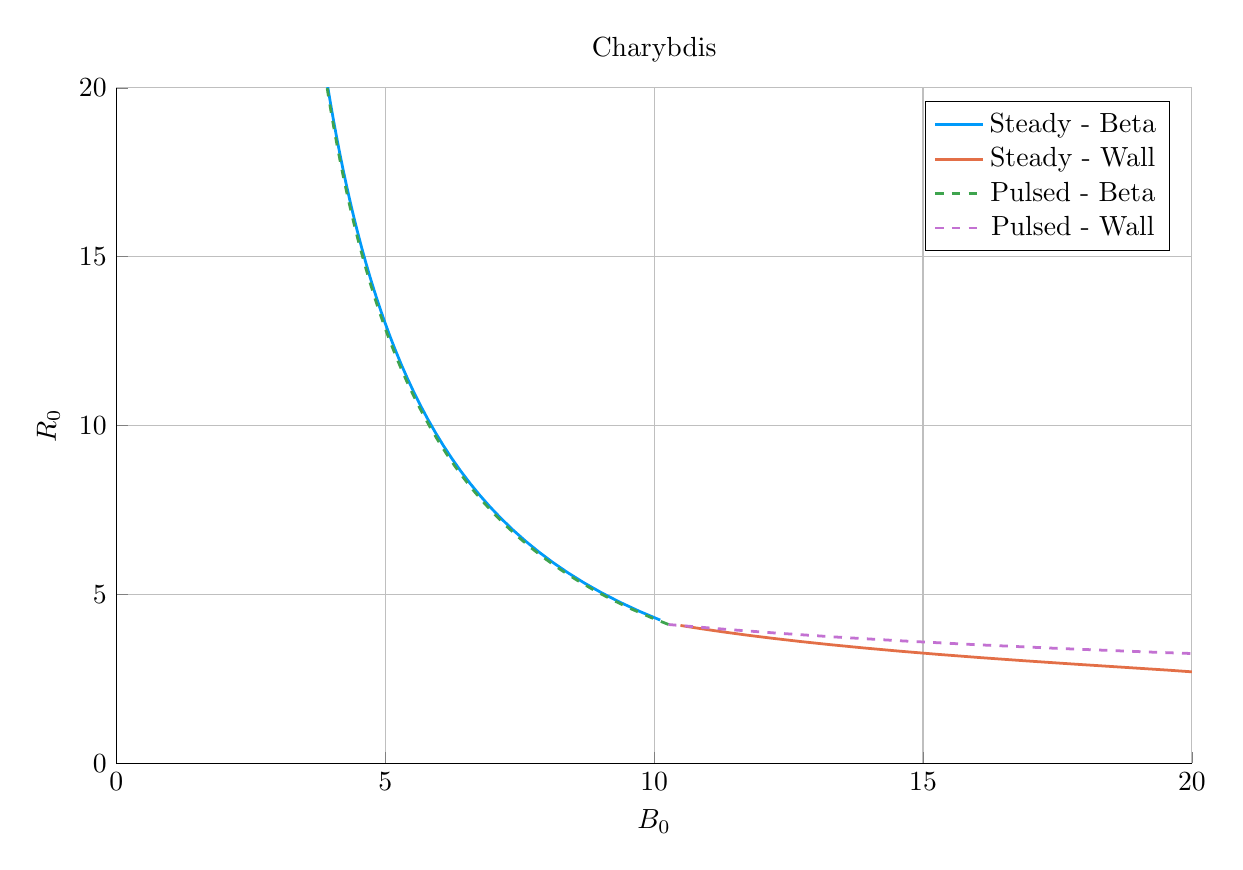
\begin{tikzpicture}[]
\begin{axis}[height = {101.6mm}, ylabel = {${R}_{0}$}, title = {Charybdis}, xmin = {0.0}, xmax = {20.0}, ymax = {20.0}, xlabel = {${B}_{0}$}, {unbounded coords=jump, scaled x ticks = false, xticklabel style={rotate = 0}, xmajorgrids = true, xtick = {0.0,5.0,10.0,15.0,20.0}, xticklabels = {0,5,10,15,20}, xtick align = inside, axis lines* = left, scaled y ticks = false, yticklabel style={rotate = 0}, ymajorgrids = true, ytick = {0.0,5.0,10.0,15.0,20.0}, yticklabels = {0,5,10,15,20}, ytick align = inside, axis lines* = left,     xshift = 0.0mm,
    yshift = 0.0mm,
    axis background/.style={fill={rgb,1:red,1.00000000;green,1.00000000;blue,1.00000000}}
, colorbar style={title=}}, ymin = {0.0}, width = {152.4mm}]\addplot+ [color = {rgb,1:red,0.00000000;green,0.60560316;blue,0.97868012},
draw opacity=1.0,
line width=1,
solid,mark = none,
mark size = 2.0,
mark options = {
    color = {rgb,1:red,0.00000000;green,0.00000000;blue,0.00000000}, draw opacity = 1.0,
    fill = {rgb,1:red,0.00000000;green,0.60560316;blue,0.97868012}, fill opacity = 1.0,
    line width = 1,
    rotate = 0,
    solid
}]coordinates {
(10.112818033153026, 4.241771689478311)
(9.722156888543116, 4.504138117525138)
(9.357875603858393, 4.77497367032698)
(9.017653755630063, 5.054228410858618)
(8.6995124437054, 5.34178832481448)
(8.401566530516865, 5.637594610921002)
(8.122163706328223, 5.941556970897918)
(7.859819415455661, 6.2535750482800845)
(7.613196557650265, 6.5735387749268055)
(7.381088038653343, 6.901328733442317)
(7.162401716104116, 7.236816533350192)
(6.956147367527331, 7.579865198961832)
(6.761425371986388, 7.930329566972662)
(6.577416849463348, 8.28805669191591)
(6.403375044688587, 8.652886257700402)
(6.2386177769852695, 9.02465099355178)
(6.0825208065966905, 9.403177092267818)
(5.934511989185341, 9.788284632344096)
(5.794066116682695, 10.179787994954152)
(5.660700347012839, 10.577496284633074)
(5.533970150598111, 10.981213744847159)
(5.413465705416883, 11.390740170754555)
(5.298808685607224, 11.805871315185586)
(5.189649392059402, 12.226399293085946)
(5.085664187259174, 12.652112975136994)
(4.986553195072601, 13.082798376170517)
(4.892038235455667, 13.518239035062717)
(4.801860966679364, 13.958216385902286)
(4.7157812114040425, 14.402510119861804)
(4.633575445956479, 14.850898537267405)
(4.5550354347559185, 15.303158889428241)
(4.479966994069385, 15.759067709846747)
(4.408188871204256, 16.21840113449116)
(4.33953172691477, 16.680935210866018)
(4.273837210246432, 17.14644619566822)
(4.210957116299974, 17.614710840865197)
(4.15075261849161, 18.085506668079862)
(4.0930935678432965, 18.558612231207235)
(4.037857852672517, 19.03380736722975)
(3.9849308127842145, 19.510873435234036)
(3.9342047029103653, 19.98959354366903)
(3.8855782007091695, 20.46975276591405)
(3.838955955133626, 20.951138344257103)
(3.7942481714200484, 21.433539882408354)
(3.7513702293348077, 21.91674952670236)
(3.710242331663442, 22.400562136158193)
(3.6707891802306123, 22.88477544159215)
(3.6329396770109583, 23.369190193993973)
(3.5966266481325166, 23.853610302391182)
(3.5617865887889004, 24.33784296144382)
(3.5283594272686503, 24.821698769019683)
(3.496288306480746, 25.30499183401733)
(3.465519381509793, 25.787539874702443)
(3.4360016318699595, 26.2691643078435)
(3.4076866872513096, 26.74969032892794)
(3.380528665662031, 27.228946983749)
(3.3544840229690007, 27.706767231660894)
(3.3295114129297314, 28.18298800079238)
(3.3055715568879336, 28.6574502355218)
(3.2826271223788512, 29.129998936506894)
(3.260642607548369, 29.600483215419466)
(3.239584247604666, 30.068756211731234)
(3.2194198921826622, 30.53467533068977)
(3.2001189373344725, 30.998102038032528)
(3.181652227422265, 31.45890197647381)
(3.163991977015565, 31.916944945395528)
(3.1471116955378684, 32.37210489697581)
(3.130986116696265, 32.82425992717794)
(3.115591132350856, 33.27329226186858)
(3.1009037305081053, 33.719088238329654)
(3.0869019371473265, 34.16153828242195)
(3.0735647616124355, 34.600536881650775)
(3.0608721453218655, 35.035982554380354)
};
\addlegendentry{Steady - Beta}
\addplot+ [color = {rgb,1:red,0.88887350;green,0.43564919;blue,0.27812294},
draw opacity=1.0,
line width=1,
solid,mark = none,
mark size = 2.0,
mark options = {
    color = {rgb,1:red,0.00000000;green,0.00000000;blue,0.00000000}, draw opacity = 1.0,
    fill = {rgb,1:red,0.88887350;green,0.43564919;blue,0.27812294}, fill opacity = 1.0,
    line width = 1,
    rotate = 0,
    solid
}]coordinates {
(20.758867641064707, 2.5885674971573294)
(20.346250098246923, 2.6701608818805265)
(19.57104597888471, 2.7580768645580767)
(18.681781921115476, 2.84914579801761)
(17.775790175980152, 2.942053074257325)
(16.896654716492492, 3.036102404206255)
(16.063927450323227, 3.1308756359103893)
(15.285557510665852, 3.226095678435203)
(14.563500533069154, 3.3215674678202314)
(13.896568848875791, 3.417147967307318)
(13.281970890030232, 3.5127292434426214)
(12.716170469467318, 3.6082281475654683)
(12.195372283741088, 3.7035796419955296)
(11.715794270833433, 3.798732281084355)
(11.273815669498969, 3.8936450383948094)
(10.866051794088186, 3.9882850129983627)
(10.489365023931143, 4.08262666943062)
};
\addlegendentry{Steady - Wall}
\addplot+ [color = {rgb,1:red,0.24222430;green,0.64327509;blue,0.30444865},
draw opacity=1.0,
line width=1,
dashed,mark = none,
mark size = 2.0,
mark options = {
    color = {rgb,1:red,0.00000000;green,0.00000000;blue,0.00000000}, draw opacity = 1.0,
    fill = {rgb,1:red,0.24222430;green,0.64327509;blue,0.30444865}, fill opacity = 1.0,
    line width = 1,
    rotate = 0,
    solid
}]coordinates {
(10.26788634689966, 4.1112515557786775)
(9.953967652326213, 4.3094639978912825)
(9.567926244368271, 4.576742787082168)
(9.207974394987358, 4.852707848855866)
(8.871841888699304, 5.137296446755483)
(8.557505525932248, 5.430432251844937)
(8.263156925406376, 5.732025498645217)
(7.9871752024348766, 6.041973183885721)
(7.728103682045175, 6.3601593098028015)
(7.484629973620137, 6.686455168691173)
(7.255568856523303, 7.020719666856628)
(7.039847526735421, 7.362799685753208)
(6.836492834698909, 7.712530477959993)
(6.644620209081183, 8.06973609553486)
(6.463424013335149, 8.43422984818008)
(6.2921691243175495, 8.80581478856818)
(6.13018355681404, 9.184284222105854)
(5.97685198655569, 9.569422237740964)
(5.831610044919842, 9.961004260702955)
(5.693939286027163, 10.358797615092055)
(5.563362729090489, 10.762562105803609)
(5.439440906144732, 11.172050607751359)
(5.321768347746793, 11.587009663771289)
(5.209970453003084, 12.007180084871303)
(5.103700692769835, 12.43229755779498)
(5.002638109938164, 12.862093246958203)
(4.906485077678376, 13.296294396161224)
(4.814965286571576, 13.734624924501638)
(4.727821933804548, 14.176806014771396)
(4.644816091323922, 14.622556692215932)
(4.565725232806084, 15.071594391671503)
(4.490341901840154, 15.523635511246878)
(4.418472505906755, 15.978395950871612)
(4.349936222622964, 16.435591634187325)
(4.284564006352339, 16.89493901242702)
(4.222197684694192, 17.3561555490841)
(4.162689135592264, 17.818960184341037)
(4.105899536872315, 18.283073778386605)
(4.051698680949713, 18.748219532911282)
(3.9999643482627323, 19.214123390225897)
(3.9505817337017928, 19.680514409594025)
(3.903442920928527, 20.147125120523665)
(3.858446400032002, 20.613691852887264)
(3.8154966244515616, 21.079955043879853)
(3.7745036035252744, 21.545659521938795)
(3.7353825273991994, 22.010554767868463)
(3.6980534213689746, 22.47439515350876)
(3.6624408270205375, 22.936940158387063)
(3.62847350780097, 23.397954564874027)
(3.5960841768845415, 23.85720863243935)
(3.565209245407392, 24.314478251672824)
(3.5357885893311605, 24.769545078785413)
(3.5077653333614305, 25.22219665136009)
(3.4810856504959875, 25.672226486155235)
(3.4556985759109375, 26.119434159797105)
(3.4315558340122845, 26.563625373217942)
(3.408611677587535, 27.004612000714285)
(3.3868227380888998, 27.44221212450356)
(3.36614788616562, 27.876250055664674)
(3.3465481016421226, 28.306556342336567)
(3.327986352208224, 28.732967766047434)
(3.3104274769652595, 29.155327355093103)
(3.2938380965241474, 29.573484219331384)
(3.278186482171801, 29.987293796610192)
(3.263442495132517, 30.396617529277517)
(3.2495774839156075, 30.801322953869263)
(3.236564206241785, 31.2012836153002)
(3.224376752844934, 31.596379002720997)
(3.212990475972638, 31.98649447963656)
(3.2023819222517877, 32.371521208907616)
(3.192528769611062, 32.751356073231776)
(3.1834097679780142, 33.12590159165121)
(3.1750046834890777, 33.49506583261046)
(3.1672942459724482, 33.8587623240416)
};
\addlegendentry{Pulsed - Beta}
\addplot+ [color = {rgb,1:red,0.76444018;green,0.44411178;blue,0.82429754},
draw opacity=1.0,
line width=1,
dashed,mark = none,
mark size = 2.0,
mark options = {
    color = {rgb,1:red,0.00000000;green,0.00000000;blue,0.00000000}, draw opacity = 1.0,
    fill = {rgb,1:red,0.76444018;green,0.44411178;blue,0.82429754}, fill opacity = 1.0,
    line width = 1,
    rotate = 0,
    solid
}]coordinates {
(48.990476413653056, 2.408463256282958)
(42.83950920694117, 2.5157944044289065)
(37.687790427214495, 2.623911121514849)
(33.33937742845888, 2.732773154793489)
(29.64296398154308, 2.8423415573543895)
(26.48039367255613, 2.9525785265823425)
(23.758442882319894, 3.0634472709719978)
(21.402860298405816, 3.174911900538905)
(19.353987387634486, 3.2869373368800954)
(17.563502020363714, 3.3994892396762393)
(15.991970371213752, 3.512533946790301)
(14.606987499719377, 3.6260384258753686)
(13.381751501116137, 3.7399702354868722)
(12.293960329570087, 3.854297494171075)
(11.32495111804522, 3.9689888562032056)
(10.459023415380802, 4.084013492866982)
(10.26788634689966, 4.1112515557786775)
};
\addlegendentry{Pulsed - Wall}
\end{axis}

\end{tikzpicture}

    \end{adjustbox}
        \caption{Charybdis Reactor}
    \end{subfigure}
    \hfill
    \begin{subfigure}[t]{0.45\textwidth}
        \centering
    \begin{adjustbox}{width=\textwidth}
      \Large
      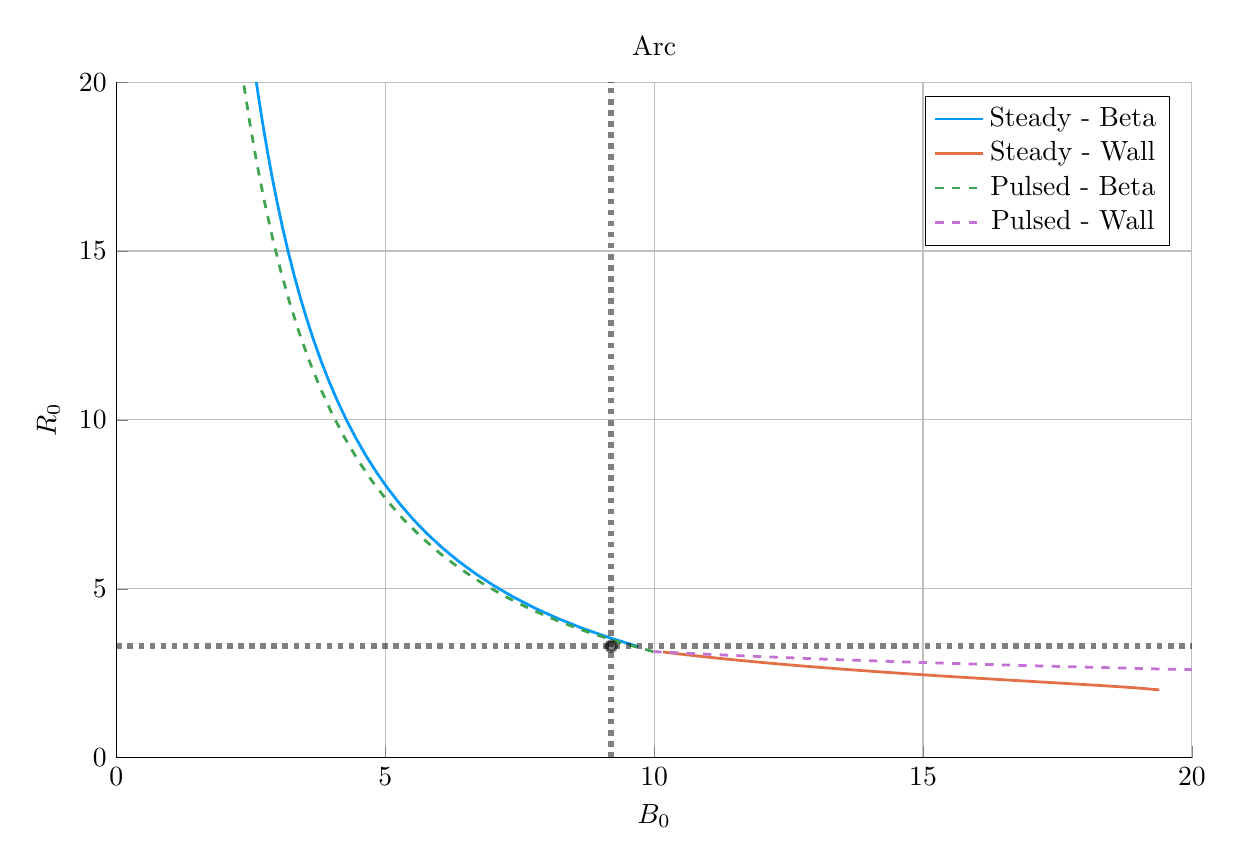
\begin{tikzpicture}[]
\begin{axis}[height = {101.6mm}, ylabel = {${R}_{0}$}, title = {Arc}, xmin = {0.0}, xmax = {20.0}, ymax = {20.0}, xlabel = {${B}_{0}$}, {unbounded coords=jump, scaled x ticks = false, xticklabel style={rotate = 0}, xmajorgrids = true, xtick = {0.0,5.0,10.0,15.0,20.0}, xticklabels = {0,5,10,15,20}, xtick align = inside, axis lines* = left, scaled y ticks = false, yticklabel style={rotate = 0}, ymajorgrids = true, ytick = {0.0,5.0,10.0,15.0,20.0}, yticklabels = {0,5,10,15,20}, ytick align = inside, axis lines* = left,     xshift = 0.0mm,
    yshift = 0.0mm,
    axis background/.style={fill={rgb,1:red,1.00000000;green,1.00000000;blue,1.00000000}}
, colorbar style={title=}}, ymin = {0.0}, width = {152.4mm}]\addplot+ [color = {rgb,1:red,0.00000000;green,0.60560316;blue,0.97868012},
draw opacity=1.0,
line width=1,
solid,mark = none,
mark size = 2.0,
mark options = {
    color = {rgb,1:red,0.00000000;green,0.00000000;blue,0.00000000}, draw opacity = 1.0,
    fill = {rgb,1:red,0.00000000;green,0.60560316;blue,0.97868012}, fill opacity = 1.0,
    line width = 1,
    rotate = 0,
    solid
}]coordinates {
(9.701206080853105, 3.2904233285656006)
(9.162315904693079, 3.553631706046861)
(8.664301107137337, 3.8315748016260343)
(8.203576462497304, 4.124583886864978)
(7.776718537485166, 4.433072975674755)
(7.380720231870917, 4.75741949036414)
(7.012886014999712, 5.097987291342331)
(6.670795005901889, 5.4551257000070565)
(6.352268997292712, 5.829168567645448)
(6.055344682097163, 6.220433393277178)
(5.778249464564785, 6.629220493040615)
(5.519380338856715, 7.05581222339423)
(5.2772854007125325, 7.500472260074458)
(5.050647625972996, 7.963444934423652)
(4.838270606140816, 8.444954628380609)
(4.639065978019038, 8.94520522910952)
(4.4520423235376105, 9.464379643936518)
(4.276295348572609, 10.002639375969222)
(4.110999177018484, 10.56012416048812)
(3.9553986195015125, 11.136951661929974)
(3.8088022956698633, 11.733217231026282)
(3.6705765055641186, 12.34899372141899)
(3.54013975965751, 12.984331364849716)
(3.4169578891619192, 13.639257703809928)
(3.30053966845824, 14.313777580345645)
(3.1904328903033052, 15.007873179535935)
(3.086220842019516, 15.721504126002731)
(2.9875191373772063, 16.45460763166718)
(2.8939728644914635, 17.207098692842226)
(2.8052540149097247, 17.97887033463821)
(2.7210591632720242, 18.7697939005645)
(2.6411073705789065, 19.579719385129263)
(2.565138287279709, 20.40847580717446)
(2.492910435164382, 21.255871621630877)
(2.4241996494611984, 22.12169516733927)
(2.3587976646588236, 23.0057151485579)
(2.296510829425685, 23.907681147764652)
(2.237158937627476, 24.827324167354146)
(2.180574163874242, 25.764357197843207)
(2.126600093288366, 26.71847581021091)
(2.075090836295778, 27.689358770027713)
(2.0259102202234582, 28.676668671060817)
(1.978931050353818, 29.68005258608471)
(1.9340344338545452, 30.69914273267572)
(1.8911091606836798, 31.733557151818793)
(1.8500511361739687, 32.78290039722107)
(1.8107628605384507, 33.846764233283025)
(1.773152951016952, 34.92472833975579)
(1.7371357028100902, 36.01636102117257)
(1.7026306853269466, 37.121219919229354)
(1.6695623706125668, 38.23885272635799)
(1.6378597911249178, 39.368797898817405)
(1.607456224302725, 40.51058536770822)
(1.5782889016090462, 41.663737246396295)
(1.5502987399539199, 42.82776853291479)
(1.5234300935954943, 44.00218780599217)
(1.4976305247952577, 45.18649791343829)
(1.4728505916614916, 46.38019665170201)
(1.4490436517578602, 47.58277743549339)
(1.4261656801829077, 48.79372995643627)
};
\addlegendentry{Steady - Beta}
\addplot+ [color = {rgb,1:red,0.88887350;green,0.43564919;blue,0.27812294},
draw opacity=1.0,
line width=1,
solid,mark = none,
mark size = 2.0,
mark options = {
    color = {rgb,1:red,0.00000000;green,0.00000000;blue,0.00000000}, draw opacity = 1.0,
    fill = {rgb,1:red,0.88887350;green,0.43564919;blue,0.27812294}, fill opacity = 1.0,
    line width = 1,
    rotate = 0,
    solid
}]coordinates {
(19.394007482712425, 2.006855814841082)
(18.932196567189358, 2.070220226465634)
(18.296989378345195, 2.1362327099649083)
(17.587029315408756, 2.2039322514902886)
(16.847882407994106, 2.272885741349308)
(16.111374502564406, 2.3427307443133163)
(15.396027314547156, 2.4132115621474344)
(14.710952688793137, 2.484165095168367)
(14.06168447794857, 2.555449485048069)
(13.450465418483889, 2.6269568263788754)
(12.877644538645335, 2.6986005527245354)
(12.342394470642008, 2.7703103261458715)
(11.843182246608265, 2.8420284550528074)
(11.376441269625893, 2.9137564749008216)
(10.944966372727551, 2.985307257194073)
(10.541663878705513, 3.056795384934831)
(10.165908182236457, 3.128148092221394)
};
\addlegendentry{Steady - Wall}
\addplot+ [color = {rgb,1:red,0.24222430;green,0.64327509;blue,0.30444865},
draw opacity=1.0,
line width=1,
dashed,mark = none,
mark size = 2.0,
mark options = {
    color = {rgb,1:red,0.00000000;green,0.00000000;blue,0.00000000}, draw opacity = 1.0,
    fill = {rgb,1:red,0.24222430;green,0.64327509;blue,0.30444865}, fill opacity = 1.0,
    line width = 1,
    rotate = 0,
    solid
}]coordinates {
(9.980483622051658, 3.1402982942956537)
(9.392786903460065, 3.3984668375583613)
(8.79273598103983, 3.7029994270206985)
(8.23820290909994, 4.029752381934837)
(7.725182218401588, 4.380005330007902)
(7.250078106370205, 4.755088191072525)
(6.80965553466646, 5.15638156809462)
(6.400998063035608, 5.585317075247801)
(6.0214713600430425, 6.043377623224966)
(5.668691517461799, 6.532097691007738)
(5.340497445229901, 7.053063624618788)
(5.034926745580058, 7.607914017422467)
(4.750194564008521, 8.198340243900201)
(4.484674995755211, 8.826087240213646)
(4.236884692979903, 9.49295465115087)
(4.00546837264544, 10.200798495308337)
(3.7891859704718387, 10.951533539957822)
(3.5869012239550364, 11.747136625739826)
(3.3975714987448393, 12.589651241396528)
(3.2202386987489797, 13.481193723261853)
(3.0540211220494466, 14.423961547290066)
(2.8981061427709687, 15.420244298711943)
(2.7517436139566023, 16.472438053930638)
(2.6142398986781377, 17.58306410230943)
(2.4849524463010138, 18.754793188384546)
(2.363284838174807, 19.990476791576892)
(2.248682232019848, 21.293187416028662)
(2.140627136740878, 22.666270490916787)
(2.038635448877246, 24.113411362836906)
(1.9422526775794744, 25.638722123308433)
(1.8510502754751532, 27.246854857488287)
(1.7646219756564088, 28.94315065234289)
(1.6825800061969869, 30.73383791051506)
(1.6045510059627948, 32.62630011975996)
(1.53017138625397, 34.629443897654504)
(1.4590817483192686, 36.754215952550474)
(1.3909197311384796, 39.01434852880224)
(1.3253102336217724, 41.42746903285954)
(1.261851128383913, 44.01681696754988)
(1.20009089049112, 46.81403058684408)
(1.1394908096975784, 49.863950342519615)
};
\addlegendentry{Pulsed - Beta}
\addplot+ [color = {rgb,1:red,0.76444018;green,0.44411178;blue,0.82429754},
draw opacity=1.0,
line width=1,
dashed,mark = none,
mark size = 2.0,
mark options = {
    color = {rgb,1:red,0.00000000;green,0.00000000;blue,0.00000000}, draw opacity = 1.0,
    fill = {rgb,1:red,0.76444018;green,0.44411178;blue,0.82429754}, fill opacity = 1.0,
    line width = 1,
    rotate = 0,
    solid
}]coordinates {
(29.27715761652869, 2.3448804182939873)
(25.4410619834368, 2.4377937236066716)
(22.158819835998365, 2.5322208586485804)
(19.342453256965573, 2.628163744265164)
(16.919364280634177, 2.7256238396687067)
(14.829378672669455, 2.8246020951898183)
(13.022412368922526, 2.9250989082568273)
(11.456617692058645, 3.0271140820266207)
(10.096901921254785, 3.1306467862637533)
(9.980483622051658, 3.1402982942956537)
};
\addlegendentry{Pulsed - Wall}
\addplot+ [color = {rgb,1:red,0.00000000;green,0.00000000;blue,0.00000000},
draw opacity=0.5,
line width=2,
dotted,mark = none,
mark size = 2.0,
mark options = {
    color = {rgb,1:red,0.00000000;green,0.00000000;blue,0.00000000}, draw opacity = 0.5,
    fill = {rgb,1:red,0.00000000;green,0.00000000;blue,0.00000000}, fill opacity = 0.5,
    line width = 1,
    rotate = 0,
    solid
},forget plot]coordinates {
(0.0, 3.3)
(20.0, 3.3)
};
\addplot+ [color = {rgb,1:red,0.00000000;green,0.00000000;blue,0.00000000},
draw opacity=0.5,
line width=2,
dotted,mark = none,
mark size = 2.0,
mark options = {
    color = {rgb,1:red,0.00000000;green,0.00000000;blue,0.00000000}, draw opacity = 0.5,
    fill = {rgb,1:red,0.00000000;green,0.00000000;blue,0.00000000}, fill opacity = 0.5,
    line width = 1,
    rotate = 0,
    solid
},forget plot]coordinates {
(9.2, 0.0)
(9.2, 20.0)
};
\addplot+[draw=none, color = {rgb,1:red,0.00000000;green,0.00000000;blue,0.00000000},
draw opacity=0.5,
line width=0,
solid,mark = *,
mark size = 2.0,
mark options = {
    color = {rgb,1:red,0.00000000;green,0.00000000;blue,0.00000000}, draw opacity = 0.5,
    fill = {rgb,1:red,0.00000000;green,0.00000000;blue,0.00000000}, fill opacity = 0.5,
    line width = 1,
    rotate = 0,
    solid
},forget plot] coordinates {
(9.2, 3.3)
};
\end{axis}

\end{tikzpicture}

    \end{adjustbox}
        \caption{Arc Reactor}
    \end{subfigure}
    \hfill \hfill ~\\ ~\\ ~\\
    \caption{Steady State Prototype Comparison} ~\\
    \label{fig:charybdis}
\end{figure*}

\begin{table}[h!]
\centering  
\caption{Charybdis Variables}
\hfill
\begin{subtable}[t]{0.4\textwidth}
\centering  
\caption{Input Variables} ~\\
\begin{tabular}{ c|c } 

Input            & Value           \\
\hline
$H$              & 1.7              \\
$Q$              & 25.0             \\
$N_{G}$          & 0.9              \\
$\epsilon$       & 0.3              \\
$\kappa_{95}$    & 1.8              \\
$\delta_{95}$    & 0.35             \\
$\nu_{n}$        & 0.4              \\
$\nu_{T}$        & 1.1              \\
$l_{i}$          & 0.5579         \\
$A$              & 2.5              \\
$Z_{eff}$        & 1.75             \\
$f_{D}$          & 0.9              \\
$\tau_{FT}$      & 1.6e9            \\
$B_{CS}$         & 12.0             \\

\end{tabular}
\end{subtable}
\hfill
\begin{subtable}[t]{0.5\textwidth}
\centering  
\caption{Output Variables} ~\\
\begin{tabular}{ c|c } 

Output           & Value       \\
\hline
$R_{0}$          & 4.13            \\
$B_{0}$          & 10.28            \\
$I_{P}$          & 8.98            \\
$\overline n$    & 1.47            \\
$\overline T$    & 15.81           \\
$\beta_{N}$       & 0.028            \\
$q_{95}$         & 6.089            \\
$P_{W}$          & 3.003            \\
$f_{BS}$         & 0.723           \\
$f_{CD}$         & 0.277           \\
$f_{ID}$         & 0.0              \\
$\volume$         & 225.5            \\
$P_{F}$          & 1294           \\
$\eta_{CD}$      & 0.291           \\

\end{tabular}
\end{subtable}
\hfill
\hfill
\end{table}

\newpage 

\subsection{Pinning down Proteus}

The pulsed twin reactor, Proteus, highlights the effects o f a high field central solenoid. When compared to the Pulsed Demo design, the $R_0$ -- $B_0$ curve looks far more favorable -- i.e. each machine built at a certain magnet strength would be more compact (and cheaper). An interesting facet of Proteus is that it exhibits all three used limits: kink safety factor, Troyon beta, and wall loading.

\begin{figure*}[h!]
    \centering
    \hfill 
    \begin{subfigure}[t]{0.45\textwidth}
        \centering
    \begin{adjustbox}{width=\textwidth}
      \Large
      \begin{tikzpicture}[]
\begin{axis}[height = {101.6mm}, ylabel = {${R}_{0}$}, title = {Proteus}, xmin = {0.0}, xmax = {20.0}, ymax = {20.0}, xlabel = {${B}_{0}$}, {unbounded coords=jump, scaled x ticks = false, xticklabel style={rotate = 0}, xmajorgrids = true, xtick = {0.0,5.0,10.0,15.0,20.0}, xticklabels = {0,5,10,15,20}, xtick align = inside, axis lines* = left, scaled y ticks = false, yticklabel style={rotate = 0}, ymajorgrids = true, ytick = {0.0,5.0,10.0,15.0,20.0}, yticklabels = {0,5,10,15,20}, ytick align = inside, axis lines* = left,     xshift = 0.0mm,
    yshift = 0.0mm,
    axis background/.style={fill={rgb,1:red,1.00000000;green,1.00000000;blue,1.00000000}}
, colorbar style={title=}}, ymin = {0.0}, width = {152.4mm}]\addplot+ [color = {rgb,1:red,0.00000000;green,0.60560316;blue,0.97868012},
draw opacity=1.0,
line width=1,
solid,mark = none,
mark size = 2.0,
mark options = {
    color = {rgb,1:red,0.00000000;green,0.00000000;blue,0.00000000}, draw opacity = 1.0,
    fill = {rgb,1:red,0.00000000;green,0.60560316;blue,0.97868012}, fill opacity = 1.0,
    line width = 1,
    rotate = 0,
    solid
}]coordinates {
(4.658732060637907, 15.19267920719026)
(4.211109766361548, 13.257359890602805)
(3.9293920326356777, 11.874737313931622)
(3.7651903683456465, 10.866007699416029)
(3.6776039543745567, 10.103021459180615)
(3.6402437753208394, 9.505760636119051)
(3.6366994671255806, 9.024418756735512)
(3.656621534643579, 8.627122931627166)
(3.693300156736026, 8.29276379316033)
(3.7422515017241134, 8.006879676976913)
(3.865532743079537, 7.5424484228595015)
(3.936096932264377, 7.350942552250971)
(4.010907188015084, 7.180521653028847)
(4.089072356933184, 7.027918062531758)
(4.169903401491354, 6.8905526178616)
(4.252857906625248, 6.7663586425757165)
(4.337501757261618, 6.653657691692545)
(4.42348218754058, 6.551070097987566)
(4.5983381267510195, 6.371833566535418)
(4.686766232902671, 6.29340795554276)
(4.775618142770625, 6.221477142908907)
(4.864743502376605, 6.155442914152805)
(4.927312314219091, 6.1123879686673135)
};
\addlegendentry{Pulsed - Kink}
\addplot+ [color = {rgb,1:red,0.88887350;green,0.43564919;blue,0.27812294},
draw opacity=1.0,
line width=1,
solid,mark = none,
mark size = 2.0,
mark options = {
    color = {rgb,1:red,0.00000000;green,0.00000000;blue,0.00000000}, draw opacity = 1.0,
    fill = {rgb,1:red,0.88887350;green,0.43564919;blue,0.27812294}, fill opacity = 1.0,
    line width = 1,
    rotate = 0,
    solid
}]coordinates {
(4.927312314219091, 6.1123879686673135)
(4.984545814413324, 6.09581207033949)
(5.17452482724068, 6.0447147858623)
(5.362091669637646, 5.999934523234248)
(5.54700293215903, 5.961033646850443)
(5.729042482638278, 5.92761240871646)
(5.908022832274664, 5.899302777254819)
(6.083785777786694, 5.87576371038825)
(6.256202341425288, 5.85667756374391)
(6.324169421042356, 5.850226299362774)
};
\addlegendentry{Pulsed - Beta}
\addplot+ [color = {rgb,1:red,0.24222430;green,0.64327509;blue,0.30444865},
draw opacity=1.0,
line width=1,
solid,mark = none,
mark size = 2.0,
mark options = {
    color = {rgb,1:red,0.00000000;green,0.00000000;blue,0.00000000}, draw opacity = 1.0,
    fill = {rgb,1:red,0.24222430;green,0.64327509;blue,0.30444865}, fill opacity = 1.0,
    line width = 1,
    rotate = 0,
    solid
}]coordinates {
(6.324169421042356, 5.850226299362774)
(6.727338549778396, 5.88388315153579)
(7.320469048424473, 5.950696360836003)
(7.835746509376305, 6.026778469060774)
(8.290245520072391, 6.109137751468495)
(8.696162676727877, 6.195913809142839)
(9.0624397222742, 6.285887257774413)
(9.395798186463841, 6.3782240354403505)
(9.701405747258567, 6.472333393687546)
(10.244760202900984, 6.664256338261126)
(10.930275827723788, 6.957604003970967)
(11.131878682735255, 7.056189303396245)
(11.50278450645086, 7.253945523825199)
(11.83715172742864, 7.452031096358636)
(11.992609772603878, 7.551070724623068)
(12.141110720831467, 7.650057379146056)
};
\addlegendentry{Pulsed - Wall}
\end{axis}

\end{tikzpicture}

    \end{adjustbox}
        \caption{Proteus Reactor}
    \end{subfigure}
    \hfill
    \begin{subfigure}[t]{0.45\textwidth}
        \centering
    \begin{adjustbox}{width=\textwidth}
      \Large
      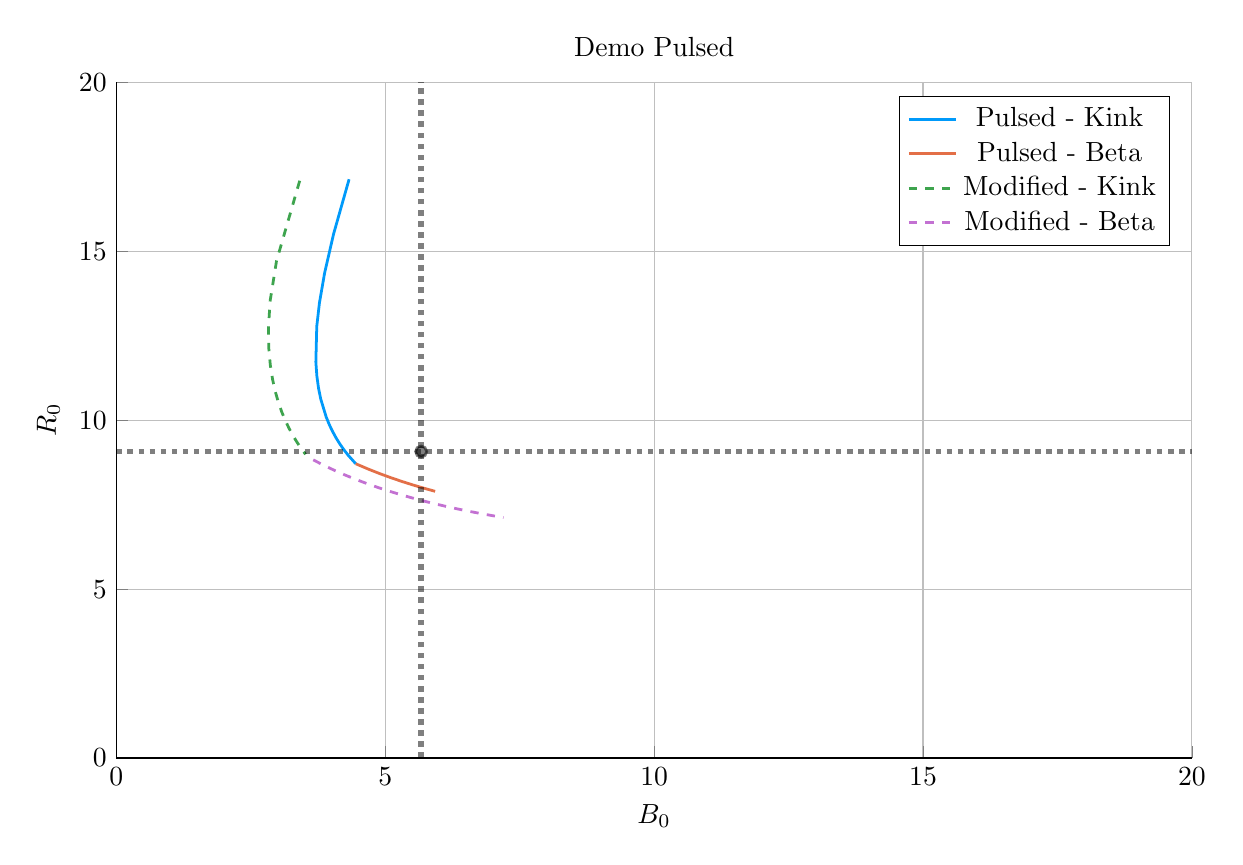
\begin{tikzpicture}[]
\begin{axis}[height = {101.6mm}, ylabel = {${R}_{0}$}, title = {Demo Pulsed}, xmin = {0.0}, xmax = {20.0}, ymax = {20.0}, xlabel = {${B}_{0}$}, {unbounded coords=jump, scaled x ticks = false, xticklabel style={rotate = 0}, xmajorgrids = true, xtick = {0.0,5.0,10.0,15.0,20.0}, xticklabels = {0,5,10,15,20}, xtick align = inside, axis lines* = left, scaled y ticks = false, yticklabel style={rotate = 0}, ymajorgrids = true, ytick = {0.0,5.0,10.0,15.0,20.0}, yticklabels = {0,5,10,15,20}, ytick align = inside, axis lines* = left,     xshift = 0.0mm,
    yshift = 0.0mm,
    axis background/.style={fill={rgb,1:red,1.00000000;green,1.00000000;blue,1.00000000}}
, colorbar style={title=}}, ymin = {0.0}, width = {152.4mm}]\addplot+ [color = {rgb,1:red,0.00000000;green,0.60560316;blue,0.97868012},
draw opacity=1.0,
line width=1,
solid,mark = none,
mark size = 2.0,
mark options = {
    color = {rgb,1:red,0.00000000;green,0.00000000;blue,0.00000000}, draw opacity = 1.0,
    fill = {rgb,1:red,0.00000000;green,0.60560316;blue,0.97868012}, fill opacity = 1.0,
    line width = 1,
    rotate = 0,
    solid
}]coordinates {
(4.327031075670194, 17.134796748649162)
(4.038214026054326, 15.511755022601415)
(3.8713719163129245, 14.355562963913712)
(3.7758613845615545, 13.476675762289453)
(3.7257856761317214, 12.778294295391971)
(3.7090473695925437, 11.723065749829066)
(3.727711597554826, 11.30970201784727)
(3.7586131667481433, 10.94971275897184)
(3.799052518631718, 10.632190690377048)
(3.901290136389271, 10.09455415135144)
(3.960577465316514, 9.863813619410237)
(4.0241209645210345, 9.653307397969705)
(4.0912717805663785, 9.460162902699798)
(4.161514602943343, 9.28206292757184)
(4.2344343960723005, 9.117114543572253)
(4.309692554546368, 8.963753917462126)
(4.450417240491067, 8.712493965092264)
};
\addlegendentry{Pulsed - Kink}
\addplot+ [color = {rgb,1:red,0.88887350;green,0.43564919;blue,0.27812294},
draw opacity=1.0,
line width=1,
solid,mark = none,
mark size = 2.0,
mark options = {
    color = {rgb,1:red,0.00000000;green,0.00000000;blue,0.00000000}, draw opacity = 1.0,
    fill = {rgb,1:red,0.88887350;green,0.43564919;blue,0.27812294}, fill opacity = 1.0,
    line width = 1,
    rotate = 0,
    solid
}]coordinates {
(4.450417240491067, 8.712493965092264)
(4.490148631384312, 8.684308742646298)
(4.692490181445514, 8.547262773806349)
(4.8960344619053355, 8.41947837460442)
(5.100651132702229, 8.30014929484307)
(5.306202822090688, 8.188581738801314)
(5.512545696627038, 8.084175191078112)
(5.719530043226767, 7.986407002697611)
(5.927000883375481, 7.894819882619234)
};
\addlegendentry{Pulsed - Beta}
\addplot+ [color = {rgb,1:red,0.24222430;green,0.64327509;blue,0.30444865},
draw opacity=1.0,
line width=1,
dashed,mark = none,
mark size = 2.0,
mark options = {
    color = {rgb,1:red,0.00000000;green,0.00000000;blue,0.00000000}, draw opacity = 1.0,
    fill = {rgb,1:red,0.24222430;green,0.64327509;blue,0.30444865}, fill opacity = 1.0,
    line width = 1,
    rotate = 0,
    solid
}]coordinates {
(3.4087424183072135, 17.090884129081292)
(2.977074181068944, 14.713048632784332)
(2.8592500074202523, 13.541171522519205)
(2.827199220063259, 12.740024138753894)
(2.8339789008667826, 12.12574468151967)
(2.862412302880871, 11.626187613249266)
(2.9044598258085443, 11.205091848948229)
(2.95577893007882, 10.841432203317366)
(3.0137895352525907, 10.521822649209419)
(3.076849710218805, 10.23716073884787)
(3.1438583711612704, 9.980947801083442)
(3.214045733980633, 9.748367275345563)
(3.2868548955983727, 9.535742205343247)
(3.361871149981842, 9.340197658526863)
(3.4387778750377818, 9.15944098345979)
(3.5173279629378453, 8.991613349767409)
};
\addlegendentry{Modified - Kink}
\addplot+ [color = {rgb,1:red,0.76444018;green,0.44411178;blue,0.82429754},
draw opacity=1.0,
line width=1,
dashed,mark = none,
mark size = 2.0,
mark options = {
    color = {rgb,1:red,0.00000000;green,0.00000000;blue,0.00000000}, draw opacity = 1.0,
    fill = {rgb,1:red,0.76444018;green,0.44411178;blue,0.82429754}, fill opacity = 1.0,
    line width = 1,
    rotate = 0,
    solid
}]coordinates {
(3.6607028750648505, 8.825949645171955)
(3.8574448036470477, 8.664618827122876)
(4.056375867871351, 8.51434867582932)
(4.257366397480293, 8.374075613831488)
(4.460279103534801, 8.242896218794312)
(4.664969389370631, 8.12003771613466)
(4.871285596007394, 8.004834914067093)
(5.07906923307514, 7.896711937521184)
(5.288155233306219, 7.795167587687744)
(5.498372259673351, 7.699763475973523)
(5.709543087166185, 7.610114306522102)
(5.921485076209294, 7.525879840414137)
(6.134010749367255, 7.446758190646709)
(6.346928478632384, 7.372480180910637)
(6.560043285872518, 7.302804563889649)
(6.773157754368795, 7.237513941672651)
(6.986073044284746, 7.176411266758267)
(7.198590001107076, 7.119316828230052)
};
\addlegendentry{Modified - Beta}
\addplot+ [color = {rgb,1:red,0.00000000;green,0.00000000;blue,0.00000000},
draw opacity=0.5,
line width=2,
dotted,mark = none,
mark size = 2.0,
mark options = {
    color = {rgb,1:red,0.00000000;green,0.00000000;blue,0.00000000}, draw opacity = 0.5,
    fill = {rgb,1:red,0.00000000;green,0.00000000;blue,0.00000000}, fill opacity = 0.5,
    line width = 1,
    rotate = 0,
    solid
},forget plot]coordinates {
(0.0, 9.072)
(20.0, 9.072)
};
\addplot+ [color = {rgb,1:red,0.00000000;green,0.00000000;blue,0.00000000},
draw opacity=0.5,
line width=2,
dotted,mark = none,
mark size = 2.0,
mark options = {
    color = {rgb,1:red,0.00000000;green,0.00000000;blue,0.00000000}, draw opacity = 0.5,
    fill = {rgb,1:red,0.00000000;green,0.00000000;blue,0.00000000}, fill opacity = 0.5,
    line width = 1,
    rotate = 0,
    solid
},forget plot]coordinates {
(5.667, 0.0)
(5.667, 20.0)
};
\addplot+[draw=none, color = {rgb,1:red,0.00000000;green,0.00000000;blue,0.00000000},
draw opacity=0.5,
line width=0,
solid,mark = *,
mark size = 2.0,
mark options = {
    color = {rgb,1:red,0.00000000;green,0.00000000;blue,0.00000000}, draw opacity = 0.5,
    fill = {rgb,1:red,0.00000000;green,0.00000000;blue,0.00000000}, fill opacity = 0.5,
    line width = 1,
    rotate = 0,
    solid
},forget plot] coordinates {
(5.667, 9.072)
};
\end{axis}

\end{tikzpicture}

    \end{adjustbox}
        \caption{Demo Pulsed Reactor}
    \end{subfigure}
    \hfill \hfill ~\\ ~\\ ~\\
    \caption{Pulsed Prototype Comparison} ~\\
\end{figure*}

\begin{table}[h!]
\centering  
\caption{Proteus Variables}
\hfill
\begin{subtable}[t]{0.4\textwidth}
\centering  
\caption{Input Variables} ~\\
\begin{tabular}{ c|c } 

Input            & Value           \\
\hline
$H$              & 1.0              \\
$Q$              & 25.0             \\
$N_{G}$          & 0.9              \\
$\epsilon$       & 0.3              \\
$\kappa_{95}$    & 1.8              \\
$\delta_{95}$    & 0.35             \\
$\nu_{n}$        & 0.4              \\
$\nu_{T}$        & 1.1              \\
$l_{i}$          & 0.6328         \\
$A$              & 2.5              \\
$Z_{eff}$        & 1.75             \\
$f_{D}$          & 0.9              \\
$\tau_{FT}$      & 7200           \\
$B_{CS}$         & 20.0             \\

\end{tabular}
\end{subtable}
\hfill
\begin{subtable}[t]{0.5\textwidth}
\centering  
\caption{Output Variables} ~\\
\begin{tabular}{ c|c } 

Output           & Value       \\
\hline
$R_{0}$          & 6.11             \\
$B_{0}$          & 4.93            \\
$I_{P}$          & 15.54            \\
$\overline n$    & 1.16            \\
$\overline T$    & 11.25            \\
$\beta_{N}$       & 0.028            \\
$q_{95}$         & 2.5              \\
$P_{W}$          & 1.763            \\
$f_{BS}$         & 0.2675           \\
$f_{CD}$         & 0.0              \\
$f_{ID}$         & 0.7325           \\
$\volume$         & 732.6            \\
$P_{F}$          & 1667           \\
$\eta_{CD}$      & 0.0              \\

\end{tabular}
\end{subtable}
\hfill
\hfill
\end{table}

\section{Learning from the Data}

Now that the model has been properly vetted and prototypes designed, we can explore how pulsed and steady-state tokamaks scale. Fitting with the Dickens theme, there will be three mostly independent results. The first result will explore how to minimize costs for a reactor by choosing optimum design points. The next will be an argument for how to properly utilize the HTS magnet technology in component design. Lastly, we will take a cursory look at the other parameters capable of lowering machine costs.

\subsection{Picking a Design Point}

With more than twenty design parameters, finding the most efficient reactor is a fool's errand. Intuition building aside, finding good reactors becomes much more feasible when only focusing on \replaced{dynamic}{floating} variables -- i.e. when keeping \replaced{static}{fixed} variables constant. This method, for example, is how all the $R_0$ -- $B_0$ curves have been produced this chapter. Once these curves are produced, it is up to the user to choose which reactor on them to build. However, the guiding metric usually involves lowering some cost, either: capital cost or cost-per-watt.

Regardless of reactor type, most efficient tokamaks operate near the beta limit -- where plasma pressure is greatest. Besides being a regime highly sensitive to magnetic field strength, the beta limit is a constraint that occurs on every reactor (seen by the authors). This beta limit is usually nested between the kink limit to lower $B_0$ values and wall loading to higher ones. Understanding these regimes is the first step towards building an intuition favoring efficient machines -- see \cref{fig:limit_regimes}.

\begin{figure}
\centering
\begin{adjustbox}{width=0.75\textwidth}
	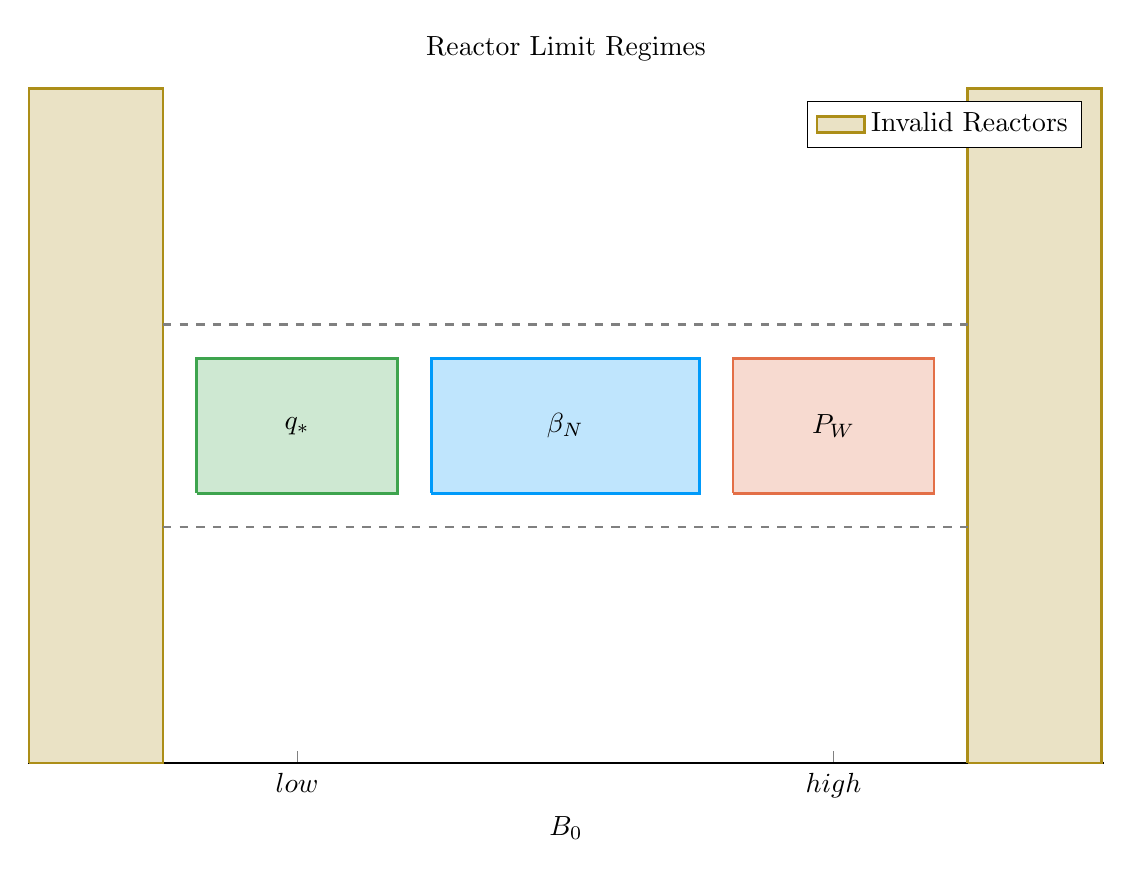
\begin{tikzpicture}[]
\begin{axis}[height = {101.6mm}, ylabel = {}, title = {Reactor Limit Regimes}, xmin = {-0.005}, xmax = {8.015}, ymax = {1.0015}, xlabel = {$B_0$}, {unbounded coords=jump, scaled x ticks = false, xticklabel style={rotate = 0}, xmajorgrids = false, xtick = {2,6}, xticklabels = {$low$,$high$}, xtick align = inside, axis lines* = left, scaled y ticks = false, yticklabel style={rotate = 0}, ymajorticks=false, ymajorgrids = false, axis lines* = left,     xshift = 0.0mm,
    yshift = 0.0mm,
    axis background/.style={fill={rgb,1:red,1.00000000;green,1.00000000;blue,1.00000000}}
, colorbar style={title=}}, ymin = {0}, width = {152.4mm}]\addplot+ [color = {rgb,1:red,0.67554396;green,0.55566233;blue,0.09423434},
draw opacity=1.0,
line width=1,
solid,mark = none,
mark size = 2.0,
mark options = {
    color = {rgb,1:red,0.00000000;green,0.00000000;blue,0.00000000}, draw opacity = 1.0,
    fill = {rgb,1:red,0.67554396;green,0.55566233;blue,0.09423434}, fill opacity = 1.0,
    line width = 1,
    rotate = 0,
    solid
},fill = {rgb,1:red,0.67554396;green,0.55566233;blue,0.09423434}, fill opacity=0.25,area legend]coordinates {
(0, 0)
(1, 0)
(1, 1)
(0, 1)
(0, 0)
};
\addlegendentry{Invalid Reactors}
\addplot+ [color = {rgb,1:red,0.67554396;green,0.55566233;blue,0.09423434},
draw opacity=1.0,
line width=1,
solid,mark = none,
mark size = 2.0,
mark options = {
    color = {rgb,1:red,0.00000000;green,0.00000000;blue,0.00000000}, draw opacity = 1.0,
    fill = {rgb,1:red,0.67554396;green,0.55566233;blue,0.09423434}, fill opacity = 1.0,
    line width = 1,
    rotate = 0,
    solid
},fill = {rgb,1:red,0.67554396;green,0.55566233;blue,0.09423434}, fill opacity=0.25,forget plot]coordinates {
(7, 0)
(8, 0)
(8, 1)
(7, 1)
(7, 0)
};
\addplot+ [color = {rgb,1:red,0.24222430;green,0.64327509;blue,0.30444865},
draw opacity=1.0,
line width=1,
solid,mark = none,
mark size = 2.0,
mark options = {
    color = {rgb,1:red,0.00000000;green,0.00000000;blue,0.00000000}, draw opacity = 1.0,
    fill = {rgb,1:red,0.24222430;green,0.64327509;blue,0.30444865}, fill opacity = 1.0,
    line width = 1,
    rotate = 0,
    solid
},fill = {rgb,1:red,0.24222430;green,0.64327509;blue,0.30444865}, fill opacity=0.25,forget plot]coordinates {
(1.25, 0.4)
(2.75, 0.4)
(2.75, 0.6)
(1.25, 0.6)
(1.25, 0.4)
};
\addplot+ [color = {rgb,1:red,0.00000000;green,0.60560316;blue,0.97868012},
draw opacity=1.0,
line width=1,
solid,mark = none,
mark size = 2.0,
mark options = {
    color = {rgb,1:red,0.00000000;green,0.00000000;blue,0.00000000}, draw opacity = 1.0,
    fill = {rgb,1:red,0.00000000;green,0.60560316;blue,0.97868012}, fill opacity = 1.0,
    line width = 1,
    rotate = 0,
    solid
},fill = {rgb,1:red,0.00000000;green,0.60560316;blue,0.97868012}, fill opacity=0.25,forget plot]coordinates {
(3.0, 0.4)
(5.0, 0.4)
(5.0, 0.6)
(3.0, 0.6)
(3.0, 0.4)
};
\addplot+ [color = {rgb,1:red,0.88887350;green,0.43564919;blue,0.27812294},
draw opacity=1.0,
line width=1,
solid,mark = none,
mark size = 2.0,
mark options = {
    color = {rgb,1:red,0.00000000;green,0.00000000;blue,0.00000000}, draw opacity = 1.0,
    fill = {rgb,1:red,0.88887350;green,0.43564919;blue,0.27812294}, fill opacity = 1.0,
    line width = 1,
    rotate = 0,
    solid
},fill = {rgb,1:red,0.88887350;green,0.43564919;blue,0.27812294}, fill opacity=0.25,forget plot]coordinates {
(5.25, 0.4)
(6.75, 0.4)
(6.75, 0.6)
(5.25, 0.6)
(5.25, 0.4)
};
\addplot+ [color = {rgb,1:red,0.50196078;green,0.50196078;blue,0.50196078},
draw opacity=1.0,
line width=1,
dashed,mark = none,
mark size = 2.0,
mark options = {
    color = {rgb,1:red,0.00000000;green,0.00000000;blue,0.00000000}, draw opacity = 1.0,
    fill = {rgb,1:red,0.50196078;green,0.50196078;blue,0.50196078}, fill opacity = 1.0,
    line width = 1,
    rotate = 0,
    solid
},forget plot]coordinates {
(1.0, 0.65)
(7.0, 0.65)
};
\addplot+ [color = {rgb,1:red,0.50196078;green,0.50196078;blue,0.50196078},
draw opacity=1.0,
line width=1,
dashed,mark = none,
mark size = 2.0,
mark options = {
    color = {rgb,1:red,0.00000000;green,0.00000000;blue,0.00000000}, draw opacity = 1.0,
    fill = {rgb,1:red,0.50196078;green,0.50196078;blue,0.50196078}, fill opacity = 1.0,
    line width = 1,
    rotate = 0,
    solid
},forget plot]coordinates {
(1.0, 0.35)
(7.0, 0.35)
};
\node at (axis cs:2, 0.5) [,
color={rgb,1:red,0.00000000;green,0.00000000;blue,0.00000000}, draw opacity=1.0,
rotate=0.0
] {$q_{*}$};
\node at (axis cs:4, 0.5) [,
color={rgb,1:red,0.00000000;green,0.00000000;blue,0.00000000}, draw opacity=1.0,
rotate=0.0
] {$\beta_N$};
\node at (axis cs:6, 0.5) [,
color={rgb,1:red,0.00000000;green,0.00000000;blue,0.00000000}, draw opacity=1.0,
rotate=0.0
] {$P_W$};
\end{axis}

\end{tikzpicture}

\end{adjustbox}
\caption{Limit Regimes as function of $B_0$}
\label{fig:limit_regimes}
\end{figure}

Now that the beta limit curve has been designated as the most efficient regime to operate in (usually), the goal is to select which reactor on it is the best one to build. Starting with the easier of the two, the optimum design point for steady-state reactors is the point where wall loading first starts to dominate design. Here, engineering concerns cause the reactor to start increasing in size and cost -- which is bad. This conclusion is justified by the cost curves for all five reactors in \cref{fig:steady_cost}. As these show, it is also where these reactor designers pinned down their tokamaks.\footnote{ Simply stated, the optimum reactor for steady-state tokamaks is one that just barely satisfies the beta and wall loading limit simultaneously -- i.e. where the two curves intersect. }

\begin{figure*}
    \centering
    \hfill 
    \begin{subfigure}[t]{0.45\textwidth}
        \centering
		\begin{adjustbox}{width=\textwidth}
			\Large
			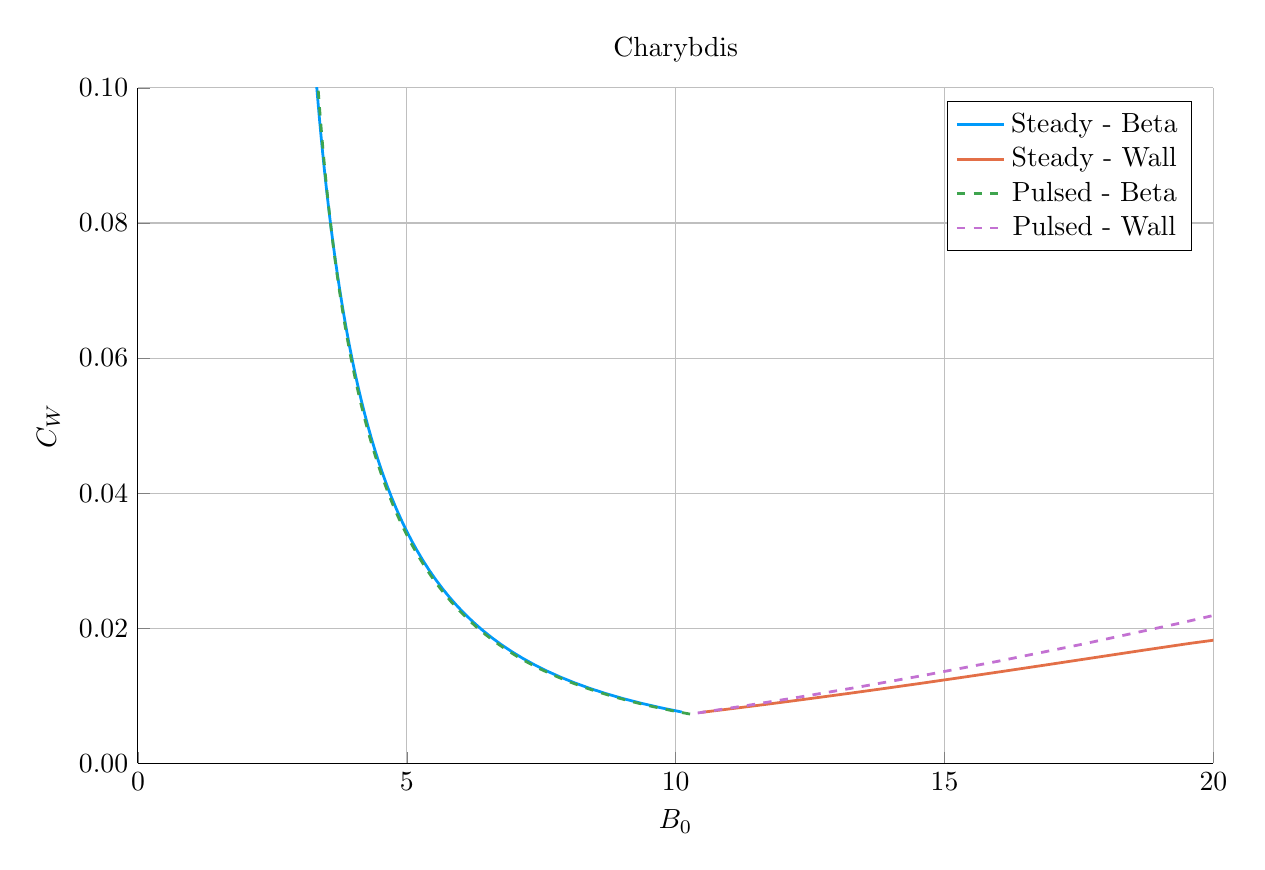
\begin{tikzpicture}[]
\begin{axis}[height = {101.6mm}, ylabel = {${C}_{W}$}, title = {Charybdis}, xmin = {0.0}, xmax = {20.0}, ymax = {0.1}, xlabel = {${B}_{0}$}, {unbounded coords=jump, scaled x ticks = false, xticklabel style={rotate = 0}, xmajorgrids = true, xtick = {0.0,5.0,10.0,15.0,20.0}, xticklabels = {0,5,10,15,20}, xtick align = inside, axis lines* = left, scaled y ticks = false, yticklabel style={rotate = 0}, ymajorgrids = true, ytick = {0.0,0.02,0.04,0.06,0.08,0.1}, yticklabels = {0.00,0.02,0.04,0.06,0.08,0.10}, ytick align = inside, axis lines* = left,     xshift = 0.0mm,
    yshift = 0.0mm,
    axis background/.style={fill={rgb,1:red,1.00000000;green,1.00000000;blue,1.00000000}}
, colorbar style={title=}}, ymin = {0.0}, width = {152.4mm}]\addplot+ [color = {rgb,1:red,0.00000000;green,0.60560316;blue,0.97868012},
draw opacity=1.0,
line width=1,
solid,mark = none,
mark size = 2.0,
mark options = {
    color = {rgb,1:red,0.00000000;green,0.00000000;blue,0.00000000}, draw opacity = 1.0,
    fill = {rgb,1:red,0.00000000;green,0.60560316;blue,0.97868012}, fill opacity = 1.0,
    line width = 1,
    rotate = 0,
    solid
}]coordinates {
(10.112818033153026, 0.007598383414978856)
(9.722156888543116, 0.008230424223188452)
(9.357875603858393, 0.008896404207575682)
(9.017653755630063, 0.009597023567402527)
(8.6995124437054, 0.010332804662622194)
(8.401566530516865, 0.011104394978990672)
(8.122163706328223, 0.011912345200844093)
(7.859819415455661, 0.012757161102175962)
(7.613196557650265, 0.013639302343912054)
(7.381088038653343, 0.014559181429827196)
(7.162401716104116, 0.015517162820285028)
(6.956147367527331, 0.016513562202290014)
(6.761425371986388, 0.017548645913683623)
(6.577416849463348, 0.018622630518712633)
(6.403375044688587, 0.019735682531644493)
(6.2386177769852695, 0.02088791828458706)
(6.0825208065966905, 0.022079403933712667)
(5.934511989185341, 0.02331015560822712)
(5.794066116682695, 0.024580139674436858)
(5.660700347012839, 0.02588927313954039)
(5.533970150598111, 0.027237424167073223)
(5.413465705416883, 0.02862441270831249)
(5.298808685607224, 0.03005001123436344)
(5.189649392059402, 0.031513945582432444)
(5.085664187259174, 0.033015895883282464)
(4.986553195072601, 0.03455549758379169)
(4.892038235455667, 0.03613234255000151)
(4.801860966679364, 0.037745980245626594)
(4.7157812114040425, 0.03939591897965519)
(4.633575445956479, 0.041081627216715676)
(4.5550354347559185, 0.04280253494397791)
(4.479966994069385, 0.04455803508845128)
(4.408188871204256, 0.046347484978679)
(4.33953172691477, 0.048170207844964834)
(4.273837210246432, 0.05002549435242988)
(4.210957116299974, 0.051912604161371986)
(4.15075261849161, 0.053830767509593334)
(4.0930935678432965, 0.05577918681155204)
(4.037857852672517, 0.05775703826940529)
(3.9849308127842145, 0.05976347349121981)
(3.9342047029103653, 0.06179762111185749)
(3.8855782007091695, 0.06385858841225403)
(3.838955955133626, 0.06594546293303978)
(3.7942481714200484, 0.06805731407868133)
(3.7513702293348077, 0.07019319470855978)
(3.710242331663442, 0.07235214271160313)
(3.6707891802306123, 0.0745331825613442)
(3.6329396770109583, 0.07673532684849063)
(3.5966266481325166, 0.07895757778829673)
(3.5617865887889004, 0.08119892870027327)
(3.5283594272686503, 0.08345836545794902)
(3.496288306480746, 0.08573486790664452)
(3.465519381509793, 0.08802741124736263)
(3.4360016318699595, 0.09033496738515884)
(3.4076866872513096, 0.0926565062404898)
(3.380528665662031, 0.09499099702224018)
(3.3544840229690007, 0.09733740946131986)
(3.3295114129297314, 0.09969471500383864)
(3.3055715568879336, 0.10206188796308927)
(3.2826271223788512, 0.10443790662966322)
(3.260642607548369, 0.10682175444066445)
(3.239584247604666, 0.10921242049746493)
(3.2194198921826622, 0.11160890156230109)
(3.2001189373344725, 0.11401020198268878)
(3.181652227422265, 0.11641533509457672)
(3.163991977015565, 0.11882332397376366)
(3.1471116955378684, 0.12123320224599504)
(3.130986116696265, 0.12364401485456963)
(3.115591132350856, 0.1260548187858383)
(3.1009037305081053, 0.12846468375306214)
(3.0869019371473265, 0.13087269283917113)
(3.0735647616124355, 0.13327794309901428)
(3.0608721453218655, 0.13567954612178545)
};
\addlegendentry{Steady - Beta}
\addplot+ [color = {rgb,1:red,0.88887350;green,0.43564919;blue,0.27812294},
draw opacity=1.0,
line width=1,
solid,mark = none,
mark size = 2.0,
mark options = {
    color = {rgb,1:red,0.00000000;green,0.00000000;blue,0.00000000}, draw opacity = 1.0,
    fill = {rgb,1:red,0.88887350;green,0.43564919;blue,0.27812294}, fill opacity = 1.0,
    line width = 1,
    rotate = 0,
    solid
}]coordinates {
(20.758867641064707, 0.018765308409143346)
(20.346250098246923, 0.018594952760163406)
(19.57104597888471, 0.01777146918538113)
(18.681781921115476, 0.016727851446155666)
(17.775790175980152, 0.015638576778075435)
(16.896654716492492, 0.014581653280825104)
(16.063927450323227, 0.013591211730165224)
(15.285557510665852, 0.012680275903338053)
(14.563500533069154, 0.01185123263968419)
(13.896568848875791, 0.01110114677254841)
(13.281970890030232, 0.010424581221258129)
(12.716170469467318, 0.009815118917575654)
(12.195372283741088, 0.00926617943914564)
(11.715794270833433, 0.008771443174384838)
(11.273815669498969, 0.008325054959037046)
(10.866051794088186, 0.007921704192505699)
(10.489365023931143, 0.007556609136513177)
};
\addlegendentry{Steady - Wall}
\addplot+ [color = {rgb,1:red,0.24222430;green,0.64327509;blue,0.30444865},
draw opacity=1.0,
line width=1,
dashed,mark = none,
mark size = 2.0,
mark options = {
    color = {rgb,1:red,0.00000000;green,0.00000000;blue,0.00000000}, draw opacity = 1.0,
    fill = {rgb,1:red,0.24222430;green,0.64327509;blue,0.30444865}, fill opacity = 1.0,
    line width = 1,
    rotate = 0,
    solid
}]coordinates {
(10.26788634689966, 0.007291637162809203)
(9.953967652326213, 0.007763018579561715)
(9.567926244368271, 0.008410560830066265)
(9.207974394987358, 0.009093056690349528)
(8.871841888699304, 0.009811202030777346)
(8.557505525932248, 0.010565644256199823)
(8.263156925406376, 0.01135697964954635)
(7.9871752024348766, 0.01218575089778548)
(7.728103682045175, 0.013052444820635726)
(7.484629973620137, 0.01395749030938975)
(7.255568856523303, 0.014901256485610468)
(7.039847526735421, 0.015884051087442074)
(6.836492834698909, 0.01690611908975986)
(6.644620209081183, 0.01796764156282338)
(6.463424013335149, 0.01906873477252413)
(6.2921691243175495, 0.020209449523749864)
(6.13018355681404, 0.02138977074682875)
(5.97685198655569, 0.022609617323612653)
(5.831610044919842, 0.023868842161338135)
(5.693939286027163, 0.025167232481888336)
(5.563362729090489, 0.026504510357656302)
(5.439440906144732, 0.0278803334592314)
(5.321768347746793, 0.02929429601917866)
(5.209970453003084, 0.030745929990983068)
(5.103700692769835, 0.03223470641747899)
(5.002638109938164, 0.03376003696406285)
(4.906485077678376, 0.03532127563010485)
(4.814965286571576, 0.03691772061565451)
(4.727821933804548, 0.03854861633202897)
(4.644816091323922, 0.04021315554278132)
(4.565725232806084, 0.04191048162126061)
(4.490341901840154, 0.04363969091085349)
(4.418472505906755, 0.04539983517396531)
(4.349936222622964, 0.047189924115870814)
(4.284564006352339, 0.049008927969770806)
(4.222197684694192, 0.05085578012965056)
(4.162689135592264, 0.05272937981792158)
(4.105899536872315, 0.05462859477526984)
(4.051698680949713, 0.056552263960658246)
(3.9999643482627323, 0.058499200250012214)
(3.9505817337017928, 0.06046819312273483)
(3.903442920928527, 0.062458011325916454)
(3.858446400032002, 0.06446740550676137)
(3.8154966244515616, 0.06649511080452623)
(3.7745036035252744, 0.06853984939399767)
(3.7353825273991994, 0.07060033297331114)
(3.6980534213689746, 0.07267526518964869)
(3.6624408270205375, 0.07476334399712868)
(3.62847350780097, 0.07686326394192533)
(3.5960841768845415, 0.07897371837037194)
(3.565209245407392, 0.08109340155652811)
(3.5357885893311605, 0.0832210107463015)
(3.5077653333614305, 0.08535524811591486)
(3.4810856504959875, 0.08749482264305544)
(3.4556985759109375, 0.08963845188964095)
(3.4315558340122845, 0.09178486369563649)
(3.408611677587535, 0.09393279778385825)
(3.3868227380888998, 0.09608100727612065)
(3.36614788616562, 0.09822826012150637)
(3.3465481016421226, 0.10037334043786662)
(3.327986352208224, 0.1025150497680155)
(3.3104274769652595, 0.10465220838353721)
(3.2938380965241474, 0.1067836557197021)
(3.278186482171801, 0.10890825269906537)
(3.263442495132517, 0.11102488135374605)
(3.2495774839156075, 0.1131324463411963)
(3.236564206241785, 0.11522987560063444)
(3.224376752844934, 0.11731612107126856)
(3.212990475972638, 0.11939015934381376)
(3.2023819222517877, 0.12145099224802183)
(3.192528769611062, 0.12349764737898258)
(3.1834097679780142, 0.1255291785649034)
(3.1750046834890777, 0.12754466627907632)
(3.1672942459724482, 0.12954321799866983)
};
\addlegendentry{Pulsed - Beta}
\addplot+ [color = {rgb,1:red,0.76444018;green,0.44411178;blue,0.82429754},
draw opacity=1.0,
line width=1,
dashed,mark = none,
mark size = 2.0,
mark options = {
    color = {rgb,1:red,0.00000000;green,0.00000000;blue,0.00000000}, draw opacity = 1.0,
    fill = {rgb,1:red,0.76444018;green,0.44411178;blue,0.82429754}, fill opacity = 1.0,
    line width = 1,
    rotate = 0,
    solid
}]coordinates {
(48.990476413653056, 0.09724163307501366)
(42.83950920694117, 0.07766994779263652)
(37.687790427214495, 0.06269593244609177)
(33.33937742845888, 0.05109841711622891)
(29.64296398154308, 0.04201539110057761)
(26.48039367255613, 0.034828857187910324)
(23.758442882319894, 0.029089432591006322)
(21.402860298405816, 0.02446606951047545)
(19.353987387634486, 0.020711961258999954)
(17.563502020363714, 0.017641064746807725)
(15.991970371213752, 0.015111701839397276)
(14.606987499719377, 0.013014953187280779)
(13.381751501116137, 0.011266342778060628)
(12.293960329570087, 0.009799811915435606)
(11.32495111804522, 0.00856330563618739)
(10.459023415380802, 0.007515507834648486)
(10.26788634689966, 0.007291637162809203)
};
\addlegendentry{Pulsed - Wall}
\end{axis}

\end{tikzpicture}

		\end{adjustbox}
        \caption{Charybdis}
    \end{subfigure}
    \hfill
    \begin{subfigure}[t]{0.45\textwidth}
        \centering
		\begin{adjustbox}{width=\textwidth}
			\Large
			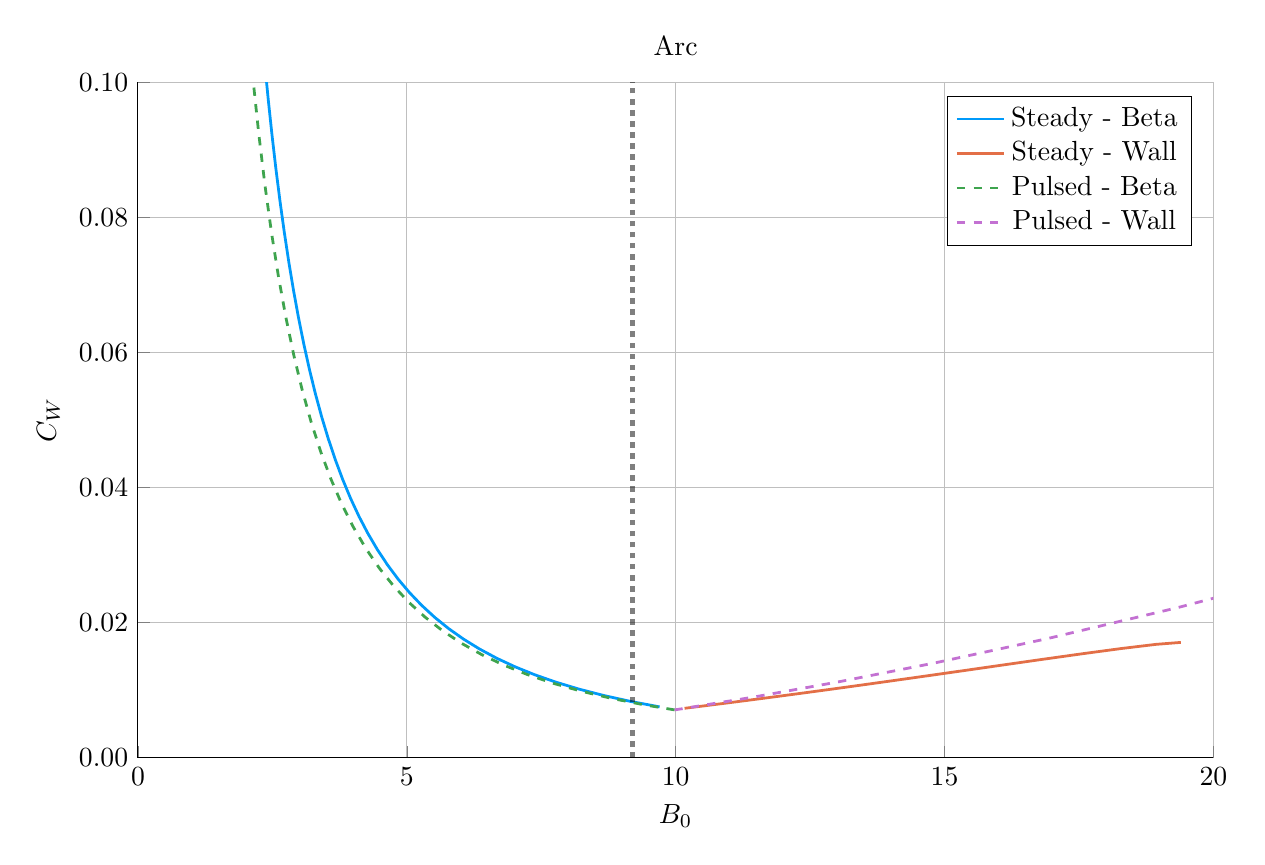
\begin{tikzpicture}[]
\begin{axis}[height = {101.6mm}, ylabel = {${C}_{W}$}, title = {Arc}, xmin = {0.0}, xmax = {20.0}, ymax = {0.1}, xlabel = {${B}_{0}$}, {unbounded coords=jump, scaled x ticks = false, xticklabel style={rotate = 0}, xmajorgrids = true, xtick = {0.0,5.0,10.0,15.0,20.0}, xticklabels = {0,5,10,15,20}, xtick align = inside, axis lines* = left, scaled y ticks = false, yticklabel style={rotate = 0}, ymajorgrids = true, ytick = {0.0,0.02,0.04,0.06,0.08,0.1}, yticklabels = {0.00,0.02,0.04,0.06,0.08,0.10}, ytick align = inside, axis lines* = left,     xshift = 0.0mm,
    yshift = 0.0mm,
    axis background/.style={fill={rgb,1:red,1.00000000;green,1.00000000;blue,1.00000000}}
, colorbar style={title=}}, ymin = {0.0}, width = {152.4mm}]\addplot+ [color = {rgb,1:red,0.00000000;green,0.60560316;blue,0.97868012},
draw opacity=1.0,
line width=1,
solid,mark = none,
mark size = 2.0,
mark options = {
    color = {rgb,1:red,0.00000000;green,0.00000000;blue,0.00000000}, draw opacity = 1.0,
    fill = {rgb,1:red,0.00000000;green,0.60560316;blue,0.97868012}, fill opacity = 1.0,
    line width = 1,
    rotate = 0,
    solid
}]coordinates {
(9.701206080853105, 0.00751651377736839)
(9.162315904693079, 0.008323905812934898)
(8.664301107137337, 0.009198905086222158)
(8.203576462497304, 0.010145151644824739)
(7.776718537485166, 0.011166668317960562)
(7.380720231870917, 0.012267478183796882)
(7.012886014999712, 0.013451673110529961)
(6.670795005901889, 0.014723405583659413)
(6.352268997292712, 0.01608688012694734)
(6.055344682097163, 0.017546344352390175)
(5.778249464564785, 0.019106079676451882)
(5.519380338856715, 0.020770391741442663)
(5.2772854007125325, 0.02254360058225732)
(5.050647625972996, 0.02443003057971548)
(4.838270606140816, 0.026434000242494555)
(4.639065978019038, 0.028559811860080504)
(4.4520423235376105, 0.030811741069328453)
(4.276295348572609, 0.03319402637711819)
(4.110999177018484, 0.03571085868120887)
(3.9553986195015125, 0.038366370830779505)
(3.8088022956698633, 0.041164627267286334)
(3.6705765055641186, 0.04410961378519341)
(3.54013975965751, 0.047205227450858)
(3.4169578891619192, 0.050455266716399376)
(3.30053966845824, 0.05386342176374704)
(3.1904328903033052, 0.05743326511231589)
(3.086220842019516, 0.061168242521834885)
(2.9875191373772063, 0.0650716642198721)
(2.8939728644914635, 0.0691466964814904)
(2.8052540149097247, 0.07339635358630757)
(2.7210591632720242, 0.07782349017600093)
(2.6411073705789065, 0.08243079403304142)
(2.565138287279709, 0.08722077929915266)
(2.492910435164382, 0.09219578014969385)
(2.4241996494611984, 0.09735794493788336)
(2.3587976646588236, 0.10270923082049731)
(2.296510829425685, 0.10825139887447487)
(2.237158937627476, 0.11398600971161459)
(2.180574163874242, 0.11991441959647205)
(2.126600093288366, 0.1260377770704313)
(2.075090836295778, 0.1323570200829707)
(2.0259102202234582, 0.13887287362917833)
(1.978931050353818, 0.14558584789074455)
(1.9340344338545452, 0.15249623687593467)
(1.8911091606836798, 0.1596041175523241)
(1.8500511361739687, 0.16690934946459546)
(1.8107628605384507, 0.17441157482817518)
(1.773152951016952, 0.1821102190881948)
(1.7371357028100902, 0.19000449193192903)
(1.7026306853269466, 0.19809338874181076)
(1.6695623706125668, 0.2063756924750063)
(1.6378597911249178, 0.21484997595463062)
(1.607456224302725, 0.22351460455684893)
(1.5782889016090462, 0.23236773927733403)
(1.5502987399539199, 0.24140734015998855)
(1.5234300935954943, 0.2506311700702061)
(1.4976305247952577, 0.26003679879456143)
(1.4728505916614916, 0.26962160744844355)
(1.4490436517578602, 0.2793827931728701)
(1.4261656801829077, 0.2893173741014787)
};
\addlegendentry{Steady - Beta}
\addplot+ [color = {rgb,1:red,0.88887350;green,0.43564919;blue,0.27812294},
draw opacity=1.0,
line width=1,
solid,mark = none,
mark size = 2.0,
mark options = {
    color = {rgb,1:red,0.00000000;green,0.00000000;blue,0.00000000}, draw opacity = 1.0,
    fill = {rgb,1:red,0.88887350;green,0.43564919;blue,0.27812294}, fill opacity = 1.0,
    line width = 1,
    rotate = 0,
    solid
}]coordinates {
(19.394007482712425, 0.017062717610395756)
(18.932196567189358, 0.01677318247708789)
(18.296989378345195, 0.01616608087020061)
(17.587029315408756, 0.015409201334794807)
(16.847882407994106, 0.014583614099307054)
(16.111374502564406, 0.01374625755936427)
(15.396027314547156, 0.012930331454144767)
(14.710952688793137, 0.012152313568351602)
(14.06168447794857, 0.011421914699879928)
(13.450465418483889, 0.010742972750322424)
(12.877644538645335, 0.010115989865118968)
(12.342394470642008, 0.009539468548127306)
(11.843182246608265, 0.00901077532361949)
(11.376441269625893, 0.008524384373336923)
(10.944966372727551, 0.008083786116178366)
(10.541663878705513, 0.007678592362816001)
(10.165908182236457, 0.0073076305932358344)
};
\addlegendentry{Steady - Wall}
\addplot+ [color = {rgb,1:red,0.24222430;green,0.64327509;blue,0.30444865},
draw opacity=1.0,
line width=1,
dashed,mark = none,
mark size = 2.0,
mark options = {
    color = {rgb,1:red,0.00000000;green,0.00000000;blue,0.00000000}, draw opacity = 1.0,
    fill = {rgb,1:red,0.24222430;green,0.64327509;blue,0.30444865}, fill opacity = 1.0,
    line width = 1,
    rotate = 0,
    solid
}]coordinates {
(9.980483622051658, 0.007070839678110688)
(9.392786903460065, 0.007852618677281367)
(8.79273598103983, 0.008801125480455354)
(8.23820290909994, 0.009848957316818736)
(7.725182218401588, 0.011005021009379608)
(7.250078106370205, 0.012278877224830715)
(6.80965553466646, 0.013680774995781924)
(6.400998063035608, 0.01522168706241675)
(6.0214713600430425, 0.01691334607316053)
(5.668691517461799, 0.01876828173242221)
(5.340497445229901, 0.020799859050557753)
(5.034926745580058, 0.02302231794191222)
(4.750194564008521, 0.02545081453735327)
(4.484674995755211, 0.028101464735781394)
(4.236884692979903, 0.030991390724248)
(4.00546837264544, 0.03413877146046793)
(3.7891859704718387, 0.03756289844971818)
(3.5869012239550364, 0.04128423857957625)
(3.3975714987448393, 0.04532450632539042)
(3.2202386987489797, 0.04970674833925621)
(3.0540211220494466, 0.05445544432876858)
(2.8981061427709687, 0.059596629277403584)
(2.7517436139566023, 0.06515804353669719)
(2.6142398986781377, 0.07116931924441194)
(2.4849524463010138, 0.07766221405391976)
(2.363284838174807, 0.08467090653190464)
(2.248682232019848, 0.09223237213933476)
(2.140627136740878, 0.10038686497222395)
(2.038635448877246, 0.10917853919500715)
(1.9422526775794744, 0.11865625658225108)
(1.8510502754751532, 0.12887464475233826)
(1.7646219756564088, 0.1398954977169483)
(1.6825800061969869, 0.15178965160557917)
(1.6045510059627948, 0.16463953300974782)
(1.53017138625397, 0.17854268160508957)
(1.4590817483192686, 0.19361672262027943)
(1.3909197311384796, 0.21000656636649426)
(1.3253102336217724, 0.22789515931839086)
(1.261851128383913, 0.24752015854836598)
(1.20009089049112, 0.2692010388315911)
(1.1394908096975784, 0.2933858656724498)
};
\addlegendentry{Pulsed - Beta}
\addplot+ [color = {rgb,1:red,0.76444018;green,0.44411178;blue,0.82429754},
draw opacity=1.0,
line width=1,
dashed,mark = none,
mark size = 2.0,
mark options = {
    color = {rgb,1:red,0.00000000;green,0.00000000;blue,0.00000000}, draw opacity = 1.0,
    fill = {rgb,1:red,0.76444018;green,0.44411178;blue,0.82429754}, fill opacity = 1.0,
    line width = 1,
    rotate = 0,
    solid
}]coordinates {
(29.27715761652869, 0.045433420664911836)
(25.4410619834368, 0.0356668159806907)
(22.158819835998365, 0.02810552804100701)
(19.342453256965573, 0.02222656993153558)
(16.919364280634177, 0.0176372518175528)
(14.829378672669455, 0.014041066675248008)
(13.022412368922526, 0.011212962182114766)
(11.456617692058645, 0.00898128637894181)
(10.096901921254785, 0.00721451699843558)
(9.980483622051658, 0.007070839678110688)
};
\addlegendentry{Pulsed - Wall}
\addplot+ [color = {rgb,1:red,0.00000000;green,0.00000000;blue,0.00000000},
draw opacity=0.5,
line width=2,
dotted,mark = none,
mark size = 2.0,
mark options = {
    color = {rgb,1:red,0.00000000;green,0.00000000;blue,0.00000000}, draw opacity = 0.5,
    fill = {rgb,1:red,0.00000000;green,0.00000000;blue,0.00000000}, fill opacity = 0.5,
    line width = 1,
    rotate = 0,
    solid
},forget plot]coordinates {
(0.0, NaN)
(20.0, NaN)
};
\addplot+ [color = {rgb,1:red,0.00000000;green,0.00000000;blue,0.00000000},
draw opacity=0.5,
line width=2,
dotted,mark = none,
mark size = 2.0,
mark options = {
    color = {rgb,1:red,0.00000000;green,0.00000000;blue,0.00000000}, draw opacity = 0.5,
    fill = {rgb,1:red,0.00000000;green,0.00000000;blue,0.00000000}, fill opacity = 0.5,
    line width = 1,
    rotate = 0,
    solid
},forget plot]coordinates {
(9.2, 0.0)
(9.2, 0.1)
};
\addplot+[draw=none, color = {rgb,1:red,0.00000000;green,0.00000000;blue,0.00000000},
draw opacity=0.5,
line width=0,
solid,mark = *,
mark size = 2.0,
mark options = {
    color = {rgb,1:red,0.00000000;green,0.00000000;blue,0.00000000}, draw opacity = 0.5,
    fill = {rgb,1:red,0.00000000;green,0.00000000;blue,0.00000000}, fill opacity = 0.5,
    line width = 1,
    rotate = 0,
    solid
},forget plot] coordinates {
(9.2, NaN)
};
\end{axis}

\end{tikzpicture}

		\end{adjustbox}
        \caption{Arc}
    \end{subfigure}
    \hfill \hfill ~\\ ~\\ ~\\ ~\\
    \hfill 
    \begin{subfigure}[t]{0.45\textwidth}
        \centering
		\begin{adjustbox}{width=\textwidth}
			\Large
			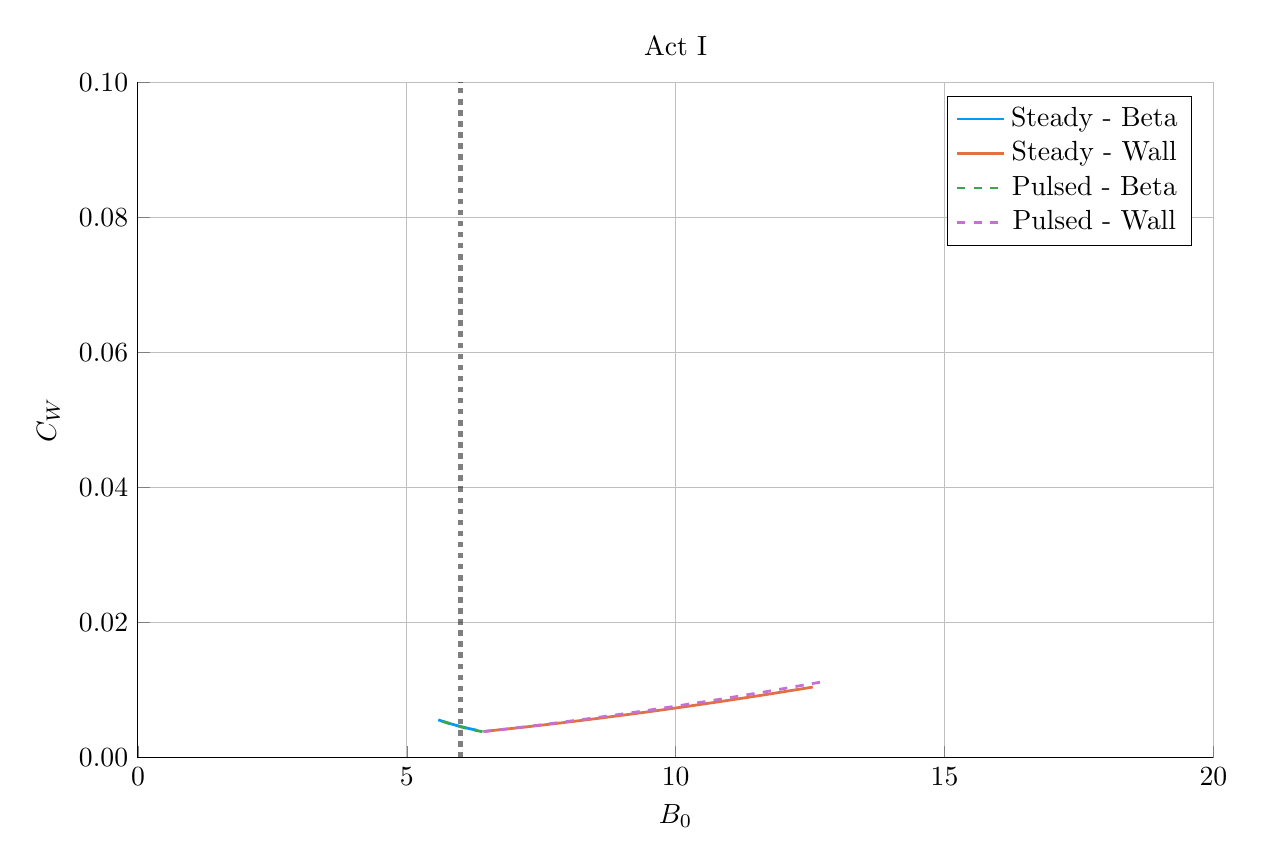
\begin{tikzpicture}[]
\begin{axis}[height = {101.6mm}, ylabel = {${C}_{W}$}, title = {Act I}, xmin = {0.0}, xmax = {20.0}, ymax = {0.1}, xlabel = {${B}_{0}$}, {unbounded coords=jump, scaled x ticks = false, xticklabel style={rotate = 0}, xmajorgrids = true, xtick = {0.0,5.0,10.0,15.0,20.0}, xticklabels = {0,5,10,15,20}, xtick align = inside, axis lines* = left, scaled y ticks = false, yticklabel style={rotate = 0}, ymajorgrids = true, ytick = {0.0,0.02,0.04,0.06,0.08,0.1}, yticklabels = {0.00,0.02,0.04,0.06,0.08,0.10}, ytick align = inside, axis lines* = left,     xshift = 0.0mm,
    yshift = 0.0mm,
    axis background/.style={fill={rgb,1:red,1.00000000;green,1.00000000;blue,1.00000000}}
, colorbar style={title=}}, ymin = {0.0}, width = {152.4mm}]\addplot+ [color = {rgb,1:red,0.00000000;green,0.60560316;blue,0.97868012},
draw opacity=1.0,
line width=1,
solid,mark = none,
mark size = 2.0,
mark options = {
    color = {rgb,1:red,0.00000000;green,0.00000000;blue,0.00000000}, draw opacity = 1.0,
    fill = {rgb,1:red,0.00000000;green,0.60560316;blue,0.97868012}, fill opacity = 1.0,
    line width = 1,
    rotate = 0,
    solid
}]coordinates {
(6.30336807958207, 0.004055552148042579)
(6.162193069273141, 0.004300298316165893)
(6.030717178404645, 0.004550498291731095)
(5.908065509576601, 0.004805976791051415)
(5.793464904530972, 0.005066558265934883)
(5.686229631357383, 0.005332067188485748)
(5.585749511271037, 0.005602328191394613)
};
\addlegendentry{Steady - Beta}
\addplot+ [color = {rgb,1:red,0.88887350;green,0.43564919;blue,0.27812294},
draw opacity=1.0,
line width=1,
solid,mark = none,
mark size = 2.0,
mark options = {
    color = {rgb,1:red,0.00000000;green,0.00000000;blue,0.00000000}, draw opacity = 1.0,
    fill = {rgb,1:red,0.88887350;green,0.43564919;blue,0.27812294}, fill opacity = 1.0,
    line width = 1,
    rotate = 0,
    solid
}]coordinates {
(12.549536249695134, 0.010450364750783054)
(11.658754653696462, 0.009311160177277214)
(10.883719833507003, 0.008367979762533702)
(10.206258129789394, 0.007581000508027489)
(9.611335769312953, 0.0069194030019139735)
(9.086446934250878, 0.006359119854353646)
(8.62129895070743, 0.0058814059200114925)
(8.207216040989662, 0.005471332591600982)
(7.837119555085499, 0.005117248050094358)
(7.505047858717157, 0.00480979217186778)
(7.20604322925957, 0.0045414928704811935)
(6.935884710193303, 0.0043062495703983395)
(6.691016583192173, 0.004099109819554263)
(6.468415485086983, 0.0039160098791423655)
};
\addlegendentry{Steady - Wall}
\addplot+ [color = {rgb,1:red,0.24222430;green,0.64327509;blue,0.30444865},
draw opacity=1.0,
line width=1,
dashed,mark = none,
mark size = 2.0,
mark options = {
    color = {rgb,1:red,0.00000000;green,0.00000000;blue,0.00000000}, draw opacity = 1.0,
    fill = {rgb,1:red,0.24222430;green,0.64327509;blue,0.30444865}, fill opacity = 1.0,
    line width = 1,
    rotate = 0,
    solid
}]coordinates {
(6.408263337806559, 0.003837054084878144)
(6.408263337806564, 0.0038370540848781357)
(6.385466513301022, 0.003872993818821736)
(6.245492502072912, 0.004106512578517519)
(6.116010320461132, 0.004344317387601225)
(5.9960421481916395, 0.004586160922256416)
(5.884727159112828, 0.004831799090393476)
(5.781304768121868, 0.00508099132781059)
(5.685100648450046, 0.005333500860613775)
(5.595515000321003, 0.005589094940610307)
};
\addlegendentry{Pulsed - Beta}
\addplot+ [color = {rgb,1:red,0.76444018;green,0.44411178;blue,0.82429754},
draw opacity=1.0,
line width=1,
dashed,mark = none,
mark size = 2.0,
mark options = {
    color = {rgb,1:red,0.00000000;green,0.00000000;blue,0.00000000}, draw opacity = 1.0,
    fill = {rgb,1:red,0.76444018;green,0.44411178;blue,0.82429754}, fill opacity = 1.0,
    line width = 1,
    rotate = 0,
    solid
}]coordinates {
(12.684248532650473, 0.011163257244949718)
(11.66307871570063, 0.009745831059904)
(10.781888309639141, 0.008590800927445573)
(10.016282491385791, 0.007639361749178777)
(9.346943280276514, 0.006847895899781745)
(8.758420158941194, 0.0061835958355957316)
(8.238241792953433, 0.005621466066992172)
(7.776255600865612, 0.005142236201168238)
(7.364131118520045, 0.0047308861724008975)
(6.994982564641668, 0.00437558945422717)
(6.66307916140573, 0.004066945929726434)
(6.408263337806559, 0.003837054084878144)
(6.408263337806564, 0.0038370540848781357)
};
\addlegendentry{Pulsed - Wall}
\addplot+ [color = {rgb,1:red,0.00000000;green,0.00000000;blue,0.00000000},
draw opacity=0.5,
line width=2,
dotted,mark = none,
mark size = 2.0,
mark options = {
    color = {rgb,1:red,0.00000000;green,0.00000000;blue,0.00000000}, draw opacity = 0.5,
    fill = {rgb,1:red,0.00000000;green,0.00000000;blue,0.00000000}, fill opacity = 0.5,
    line width = 1,
    rotate = 0,
    solid
},forget plot]coordinates {
(0.0, NaN)
(20.0, NaN)
};
\addplot+ [color = {rgb,1:red,0.00000000;green,0.00000000;blue,0.00000000},
draw opacity=0.5,
line width=2,
dotted,mark = none,
mark size = 2.0,
mark options = {
    color = {rgb,1:red,0.00000000;green,0.00000000;blue,0.00000000}, draw opacity = 0.5,
    fill = {rgb,1:red,0.00000000;green,0.00000000;blue,0.00000000}, fill opacity = 0.5,
    line width = 1,
    rotate = 0,
    solid
},forget plot]coordinates {
(6.0, 0.0)
(6.0, 0.1)
};
\addplot+[draw=none, color = {rgb,1:red,0.00000000;green,0.00000000;blue,0.00000000},
draw opacity=0.5,
line width=0,
solid,mark = *,
mark size = 2.0,
mark options = {
    color = {rgb,1:red,0.00000000;green,0.00000000;blue,0.00000000}, draw opacity = 0.5,
    fill = {rgb,1:red,0.00000000;green,0.00000000;blue,0.00000000}, fill opacity = 0.5,
    line width = 1,
    rotate = 0,
    solid
},forget plot] coordinates {
(6.0, NaN)
};
\end{axis}

\end{tikzpicture}

		\end{adjustbox}
        \caption{Act I}
    \end{subfigure}
    \hfill
    \begin{subfigure}[t]{0.45\textwidth}
        \centering
		\begin{adjustbox}{width=\textwidth}
			\Large
			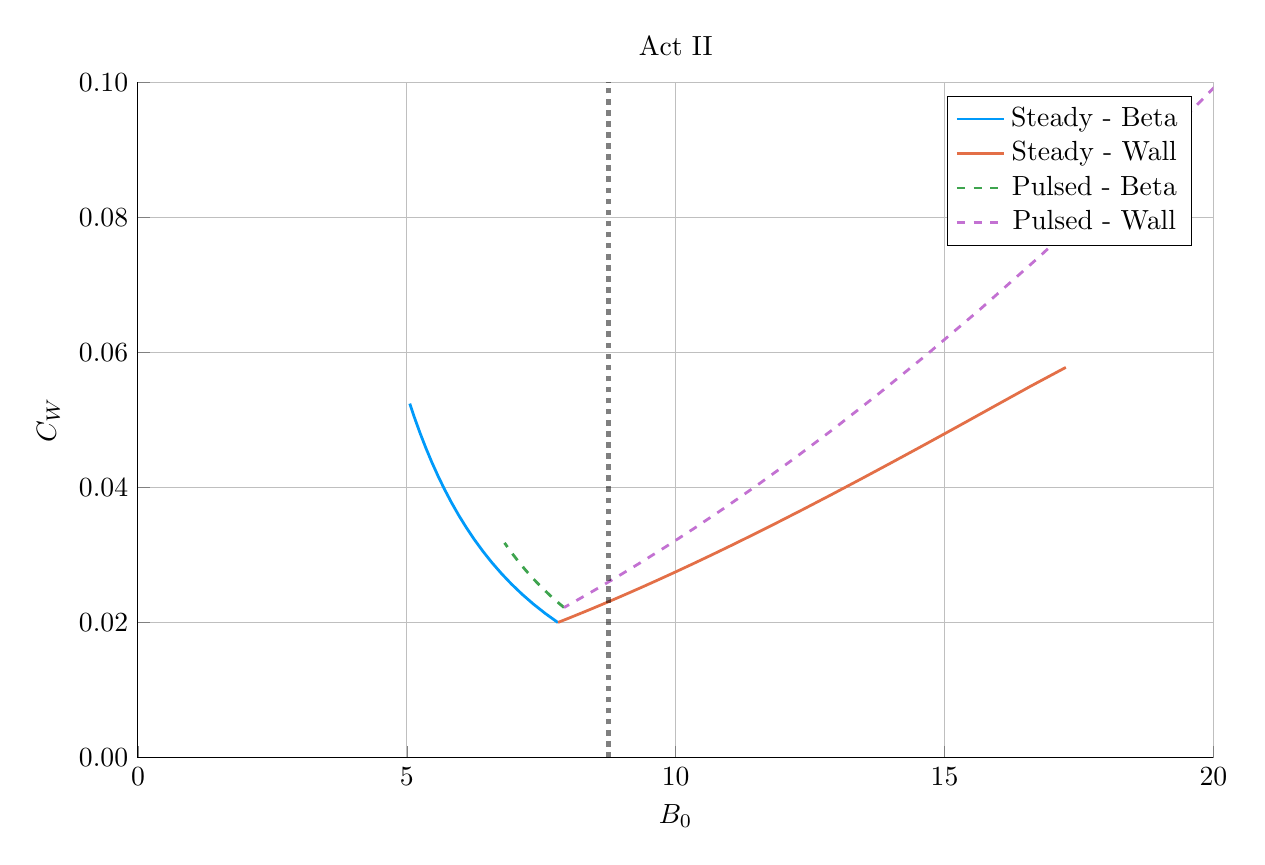
\begin{tikzpicture}[]
\begin{axis}[height = {101.6mm}, ylabel = {${C}_{W}$}, title = {Act II}, xmin = {0.0}, xmax = {20.0}, ymax = {0.1}, xlabel = {${B}_{0}$}, {unbounded coords=jump, scaled x ticks = false, xticklabel style={rotate = 0}, xmajorgrids = true, xtick = {0.0,5.0,10.0,15.0,20.0}, xticklabels = {0,5,10,15,20}, xtick align = inside, axis lines* = left, scaled y ticks = false, yticklabel style={rotate = 0}, ymajorgrids = true, ytick = {0.0,0.02,0.04,0.06,0.08,0.1}, yticklabels = {0.00,0.02,0.04,0.06,0.08,0.10}, ytick align = inside, axis lines* = left,     xshift = 0.0mm,
    yshift = 0.0mm,
    axis background/.style={fill={rgb,1:red,1.00000000;green,1.00000000;blue,1.00000000}}
, colorbar style={title=}}, ymin = {0.0}, width = {152.4mm}]\addplot+ [color = {rgb,1:red,0.00000000;green,0.60560316;blue,0.97868012},
draw opacity=1.0,
line width=1,
solid,mark = none,
mark size = 2.0,
mark options = {
    color = {rgb,1:red,0.00000000;green,0.00000000;blue,0.00000000}, draw opacity = 1.0,
    fill = {rgb,1:red,0.00000000;green,0.60560316;blue,0.97868012}, fill opacity = 1.0,
    line width = 1,
    rotate = 0,
    solid
}]coordinates {
(7.810935944285959, 0.019999870342781445)
(7.57736049850867, 0.02133467083845229)
(7.354864292609041, 0.022732819748494743)
(7.145167234136329, 0.024185030975062572)
(6.9473303865083675, 0.025691491983248542)
(6.760499508614096, 0.027252320661142464)
(6.583897990324067, 0.028867554534578326)
(6.416817229618043, 0.030537157829042417)
(6.258609820663305, 0.032261020375438675)
(6.108683264880386, 0.034038958296321455)
(5.966494431410919, 0.03587071487617403)
(5.831544666176381, 0.0377559616009066)
(5.703375459679132, 0.03969429938840844)
(5.581564609582325, 0.04168525992229865)
(5.465722802994068, 0.04372830718110872)
(5.355490573482678, 0.04582283908419109)
(5.25053558682053, 0.047968189231402746)
(5.1505502068221745, 0.0501636288266544)
(5.0552493196883175, 0.0524083686363995)
};
\addlegendentry{Steady - Beta}
\addplot+ [color = {rgb,1:red,0.88887350;green,0.43564919;blue,0.27812294},
draw opacity=1.0,
line width=1,
solid,mark = none,
mark size = 2.0,
mark options = {
    color = {rgb,1:red,0.00000000;green,0.00000000;blue,0.00000000}, draw opacity = 1.0,
    fill = {rgb,1:red,0.88887350;green,0.43564919;blue,0.27812294}, fill opacity = 1.0,
    line width = 1,
    rotate = 0,
    solid
}]coordinates {
(17.25550839059296, 0.057778872694714996)
(16.594334962335296, 0.05496298917461432)
(15.9071755430688, 0.05194082278283737)
(15.233983138507648, 0.04897170009560995)
(14.594239858921854, 0.04617848140750687)
(13.989673082630297, 0.04357183498888427)
(13.414782495717416, 0.041119354314331134)
(12.872659546281994, 0.03883879592226187)
(12.364365715508608, 0.03673485145929315)
(11.889507953196574, 0.03480335845855904)
(11.44685939646348, 0.0330353994524836)
(11.034739998180656, 0.03141974653036777)
(10.651252523287319, 0.02994431754557875)
(10.294428800132035, 0.02859703023052943)
(9.962319203963213, 0.02736628585076568)
(9.653045819449929, 0.0262412244397216)
(9.364832254395445, 0.02521184000785315)
(9.096018465506306, 0.02426901119368965)
(8.844373144802077, 0.023401030424376988)
(8.61055754360846, 0.022610816631964757)
(8.391192178573277, 0.021881336042883122)
(8.18577947665566, 0.021210054866812295)
(7.99323348423048, 0.020591621521449808)
(7.812301489248497, 0.02001998340874561)
};
\addlegendentry{Steady - Wall}
\addplot+ [color = {rgb,1:red,0.24222430;green,0.64327509;blue,0.30444865},
draw opacity=1.0,
line width=1,
dashed,mark = none,
mark size = 2.0,
mark options = {
    color = {rgb,1:red,0.00000000;green,0.00000000;blue,0.00000000}, draw opacity = 1.0,
    fill = {rgb,1:red,0.24222430;green,0.64327509;blue,0.30444865}, fill opacity = 1.0,
    line width = 1,
    rotate = 0,
    solid
}]coordinates {
(7.923668284887995, 0.02222721640664124)
(7.923668284887995, 0.022227216406641305)
(7.836759696043437, 0.022801804106215327)
(7.6662731560983355, 0.023999703560063156)
(7.50499428233835, 0.025227714472706875)
(7.35232773269976, 0.026485173676255868)
(7.207727224738343, 0.02777136956552452)
(7.070690693175276, 0.029085544281911353)
(6.940756001029682, 0.03042689602188544)
(6.817497143644154, 0.0317945813900804)
};
\addlegendentry{Pulsed - Beta}
\addplot+ [color = {rgb,1:red,0.76444018;green,0.44411178;blue,0.82429754},
draw opacity=1.0,
line width=1,
dashed,mark = none,
mark size = 2.0,
mark options = {
    color = {rgb,1:red,0.00000000;green,0.00000000;blue,0.00000000}, draw opacity = 1.0,
    fill = {rgb,1:red,0.76444018;green,0.44411178;blue,0.82429754}, fill opacity = 1.0,
    line width = 1,
    rotate = 0,
    solid
}]coordinates {
(22.56106430311702, 0.12077728813238993)
(20.85607192394036, 0.10611249618735387)
(19.335265246056654, 0.09369703436900484)
(17.974121547130903, 0.08312792497015177)
(16.751976718553127, 0.07408393734926945)
(15.651329744019142, 0.06630720048423838)
(14.65728744097675, 0.05958933132558854)
(13.757118584462601, 0.05376088392733976)
(12.939893642194303, 0.04868326015323384)
(12.196191964860315, 0.04424246074454113)
(11.517862472405039, 0.04034422355142677)
(10.897827027335556, 0.0369102154096456)
(10.329918077124672, 0.0338750302375444)
(9.808743940706389, 0.031183808185534914)
(9.329576544487265, 0.02879033654896873)
(8.888257451278507, 0.026655526551708646)
(8.481118883411932, 0.024746185235479588)
(8.10491708701527, 0.02303402032897385)
(7.923668284887995, 0.02222721640664124)
(7.923668284887995, 0.022227216406641305)
};
\addlegendentry{Pulsed - Wall}
\addplot+ [color = {rgb,1:red,0.00000000;green,0.00000000;blue,0.00000000},
draw opacity=0.5,
line width=2,
dotted,mark = none,
mark size = 2.0,
mark options = {
    color = {rgb,1:red,0.00000000;green,0.00000000;blue,0.00000000}, draw opacity = 0.5,
    fill = {rgb,1:red,0.00000000;green,0.00000000;blue,0.00000000}, fill opacity = 0.5,
    line width = 1,
    rotate = 0,
    solid
},forget plot]coordinates {
(0.0, NaN)
(20.0, NaN)
};
\addplot+ [color = {rgb,1:red,0.00000000;green,0.00000000;blue,0.00000000},
draw opacity=0.5,
line width=2,
dotted,mark = none,
mark size = 2.0,
mark options = {
    color = {rgb,1:red,0.00000000;green,0.00000000;blue,0.00000000}, draw opacity = 0.5,
    fill = {rgb,1:red,0.00000000;green,0.00000000;blue,0.00000000}, fill opacity = 0.5,
    line width = 1,
    rotate = 0,
    solid
},forget plot]coordinates {
(8.75, 0.0)
(8.75, 0.1)
};
\addplot+[draw=none, color = {rgb,1:red,0.00000000;green,0.00000000;blue,0.00000000},
draw opacity=0.5,
line width=0,
solid,mark = *,
mark size = 2.0,
mark options = {
    color = {rgb,1:red,0.00000000;green,0.00000000;blue,0.00000000}, draw opacity = 0.5,
    fill = {rgb,1:red,0.00000000;green,0.00000000;blue,0.00000000}, fill opacity = 0.5,
    line width = 1,
    rotate = 0,
    solid
},forget plot] coordinates {
(8.75, NaN)
};
\end{axis}

\end{tikzpicture}

		\end{adjustbox}
        \caption{Act II}
    \end{subfigure}
    \hfill \hfill ~\\ ~\\ ~\\
    \caption{Steady State Cost Curves}
    \label{fig:steady_cost}
\end{figure*}

The problem of selecting an optimum design is more difficult for the pulsed case. This is mainly due to the kink limit regime being actually achievable. Following the conclusion from steady-state reactors would be an oversimplification because there are actually two costs relevant to a reactor: capital cost and cost-per-watt. These beta-wall reactors are actually the points often best for minimizing cost-per-watt (i.e. your rate of return). The new beta-kink reactors, then, lead to cheap to build machines -- as they minimize capital cost. These conclusions are shown in \cref{fig:pulsed_costs}.

\begin{figure*}
    \centering
    \hfill 
    \begin{subfigure}[t]{0.45\textwidth}
        \centering
		\begin{adjustbox}{width=\textwidth}
			\Large
			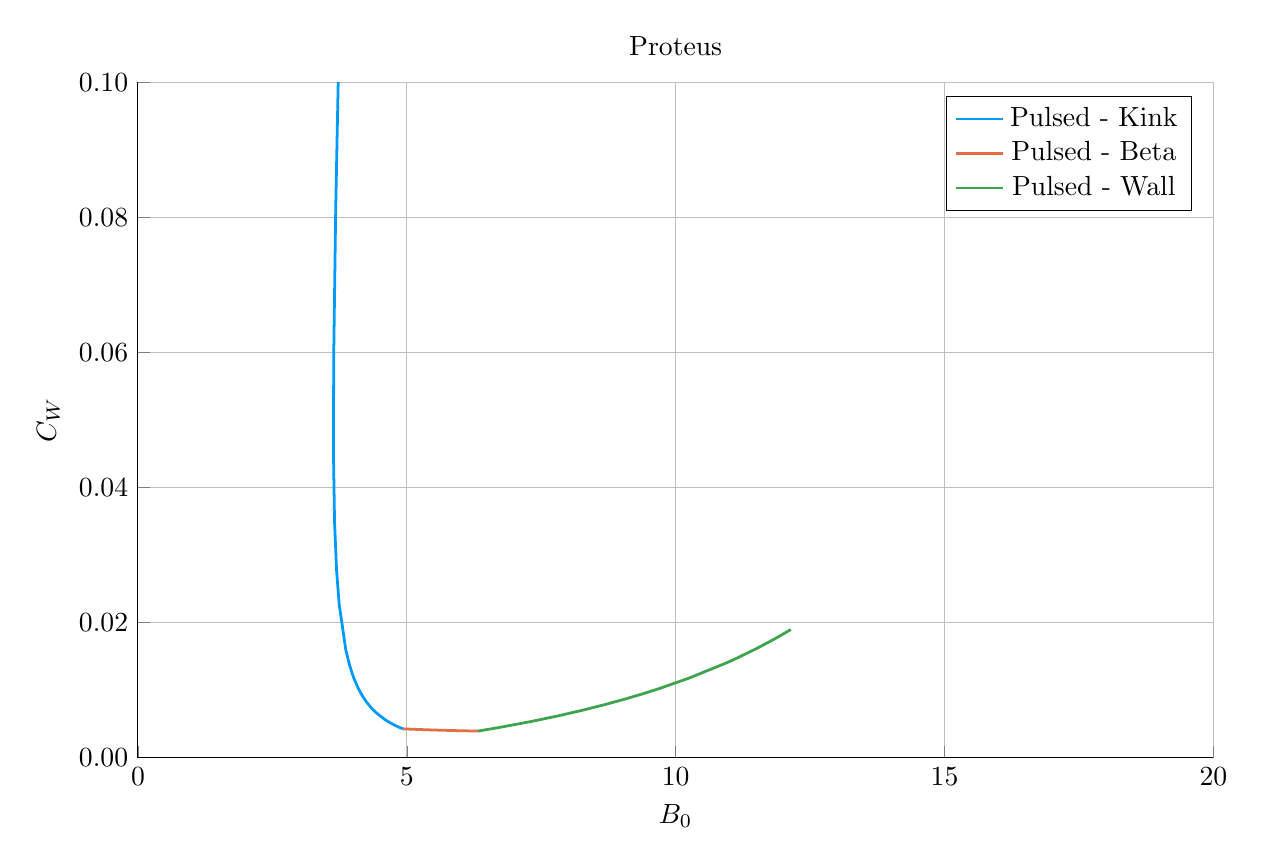
\begin{tikzpicture}[]
\begin{axis}[height = {101.6mm}, ylabel = {${C}_{W}$}, title = {Proteus}, xmin = {0.0}, xmax = {20.0}, ymax = {0.1}, xlabel = {${B}_{0}$}, {unbounded coords=jump, scaled x ticks = false, xticklabel style={rotate = 0}, xmajorgrids = true, xtick = {0.0,5.0,10.0,15.0,20.0}, xticklabels = {0,5,10,15,20}, xtick align = inside, axis lines* = left, scaled y ticks = false, yticklabel style={rotate = 0}, ymajorgrids = true, ytick = {0.0,0.02,0.04,0.06,0.08,0.1}, yticklabels = {0.00,0.02,0.04,0.06,0.08,0.10}, ytick align = inside, axis lines* = left,     xshift = 0.0mm,
    yshift = 0.0mm,
    axis background/.style={fill={rgb,1:red,1.00000000;green,1.00000000;blue,1.00000000}}
, colorbar style={title=}}, ymin = {0.0}, width = {152.4mm}]\addplot+ [color = {rgb,1:red,0.00000000;green,0.60560316;blue,0.97868012},
draw opacity=1.0,
line width=1,
solid,mark = none,
mark size = 2.0,
mark options = {
    color = {rgb,1:red,0.00000000;green,0.00000000;blue,0.00000000}, draw opacity = 1.0,
    fill = {rgb,1:red,0.00000000;green,0.60560316;blue,0.97868012}, fill opacity = 1.0,
    line width = 1,
    rotate = 0,
    solid
}]coordinates {
(4.658732060637907, 0.5238680720960677)
(4.211109766361548, 0.29158377814463826)
(3.9293920326356777, 0.17767190497429325)
(3.7651903683456465, 0.1166072358238225)
(3.6776039543745567, 0.08112372927887979)
(3.6402437753208394, 0.05909652489757084)
(3.6366994671255806, 0.04467306876996977)
(3.656621534643579, 0.03480923074663025)
(3.693300156736026, 0.02781736023114741)
(3.7422515017241134, 0.022710208007687336)
(3.865532743079537, 0.015952709019313158)
(3.936096932264377, 0.013665127664349888)
(4.010907188015084, 0.01184965388633812)
(4.089072356933184, 0.010387577045642686)
(4.169903401491354, 0.009194676609194867)
(4.252857906625248, 0.008210013517334984)
(4.337501757261618, 0.007388710643319612)
(4.42348218754058, 0.006697190814676216)
(4.5983381267510195, 0.005607443376267891)
(4.686766232902671, 0.005174363801875551)
(4.775618142770625, 0.004798727872321348)
(4.864743502376605, 0.004470996685456748)
(4.927312314219091, 0.004265648977267023)
};
\addlegendentry{Pulsed - Kink}
\addplot+ [color = {rgb,1:red,0.88887350;green,0.43564919;blue,0.27812294},
draw opacity=1.0,
line width=1,
solid,mark = none,
mark size = 2.0,
mark options = {
    color = {rgb,1:red,0.00000000;green,0.00000000;blue,0.00000000}, draw opacity = 1.0,
    fill = {rgb,1:red,0.88887350;green,0.43564919;blue,0.27812294}, fill opacity = 1.0,
    line width = 1,
    rotate = 0,
    solid
}]coordinates {
(4.927312314219091, 0.004265648977267023)
(4.984545814413324, 0.004246004028390513)
(5.17452482724068, 0.0041849470602593405)
(5.362091669637646, 0.0041306604637180565)
(5.54700293215903, 0.004082678433657853)
(5.729042482638278, 0.004040568150841258)
(5.908022832274664, 0.004003927180150204)
(6.083785777786694, 0.003972381072297988)
(6.256202341425288, 0.003945581215430235)
(6.324169421042356, 0.003936121998618512)
};
\addlegendentry{Pulsed - Beta}
\addplot+ [color = {rgb,1:red,0.24222430;green,0.64327509;blue,0.30444865},
draw opacity=1.0,
line width=1,
solid,mark = none,
mark size = 2.0,
mark options = {
    color = {rgb,1:red,0.00000000;green,0.00000000;blue,0.00000000}, draw opacity = 1.0,
    fill = {rgb,1:red,0.24222430;green,0.64327509;blue,0.30444865}, fill opacity = 1.0,
    line width = 1,
    rotate = 0,
    solid
}]coordinates {
(6.324169421042356, 0.003936121998618512)
(6.727338549778396, 0.004479602725986452)
(7.320469048424473, 0.005364564868057796)
(7.835746509376305, 0.006224935802002464)
(8.290245520072391, 0.007063234029306885)
(8.696162676727877, 0.00788223849893927)
(9.0624397222742, 0.00868451845222651)
(9.395798186463841, 0.00947231261660997)
(9.701405747258567, 0.010247527923592582)
(10.244760202900984, 0.011766415534875542)
(10.930275827723788, 0.013983337609097824)
(11.131878682735255, 0.014709436843559874)
(11.50278450645086, 0.01614615622924262)
(11.83715172742864, 0.017565397423788643)
(11.992609772603878, 0.018269423189653803)
(12.141110720831467, 0.018970135151011147)
};
\addlegendentry{Pulsed - Wall}
\end{axis}

\end{tikzpicture}

		\end{adjustbox}
        \caption{Proteus Cost-per-Watt}
    \end{subfigure}
    \hfill
    \begin{subfigure}[t]{0.45\textwidth}
        \centering
		\begin{adjustbox}{width=\textwidth}
			\Large
			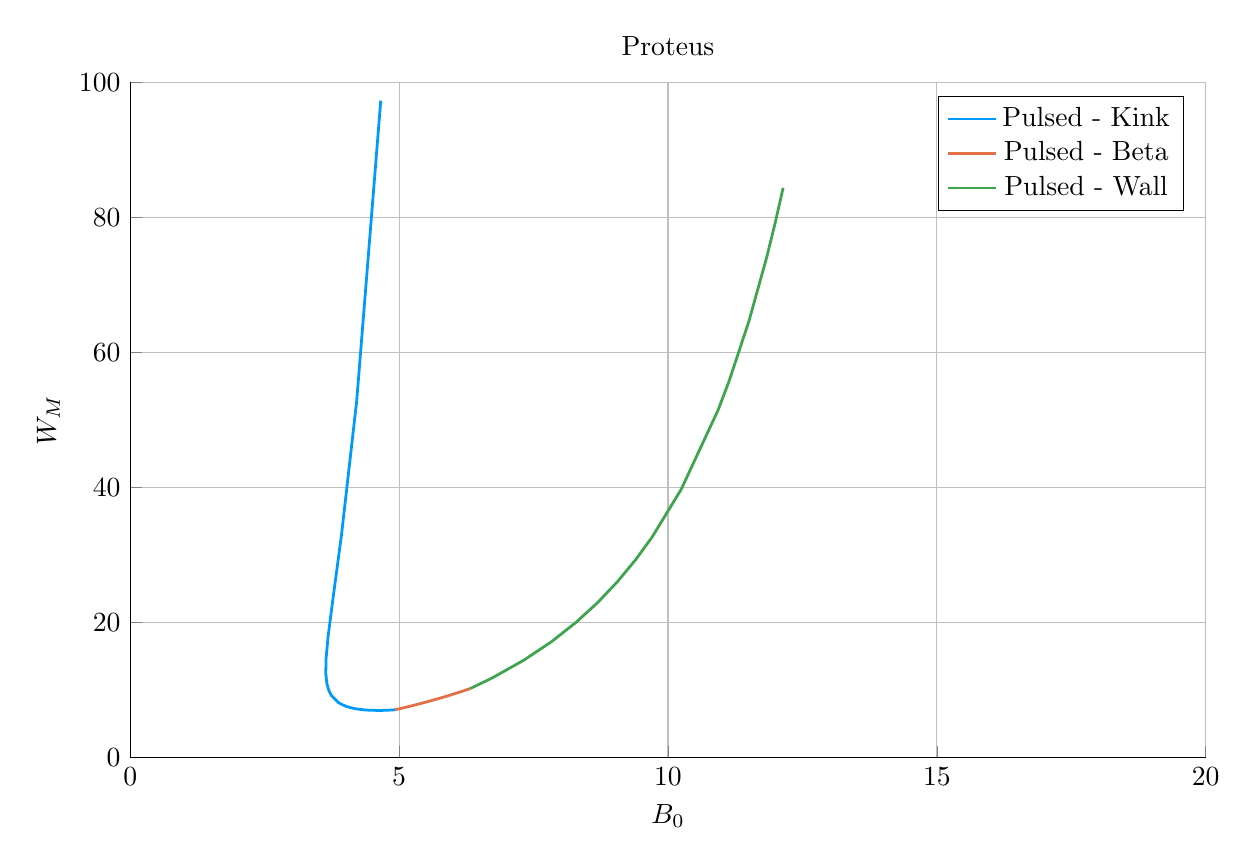
\begin{tikzpicture}[]
\begin{axis}[height = {101.6mm}, ylabel = {${W}_{M}$}, title = {Proteus}, xmin = {0.0}, xmax = {20.0}, ymax = {100.0}, xlabel = {${B}_{0}$}, {unbounded coords=jump, scaled x ticks = false, xticklabel style={rotate = 0}, xmajorgrids = true, xtick = {0.0,5.0,10.0,15.0,20.0}, xticklabels = {0,5,10,15,20}, xtick align = inside, axis lines* = left, scaled y ticks = false, yticklabel style={rotate = 0}, ymajorgrids = true, ytick = {0.0,20.0,40.0,60.0,80.0,100.0}, yticklabels = {0,20,40,60,80,100}, ytick align = inside, axis lines* = left,     xshift = 0.0mm,
    yshift = 0.0mm,
    axis background/.style={fill={rgb,1:red,1.00000000;green,1.00000000;blue,1.00000000}}
, colorbar style={title=}}, ymin = {0.0}, width = {152.4mm}]\addplot+ [color = {rgb,1:red,0.00000000;green,0.60560316;blue,0.97868012},
draw opacity=1.0,
line width=1,
solid,mark = none,
mark size = 2.0,
mark options = {
    color = {rgb,1:red,0.00000000;green,0.00000000;blue,0.00000000}, draw opacity = 1.0,
    fill = {rgb,1:red,0.00000000;green,0.60560316;blue,0.97868012}, fill opacity = 1.0,
    line width = 1,
    rotate = 0,
    solid
}]coordinates {
(4.658732060637907, 97.28232425378617)
(4.211109766361548, 52.81528522659042)
(3.9293920326356777, 33.045940900779435)
(3.7651903683456465, 23.247661382566328)
(3.6776039543745567, 17.827034690374397)
(3.6402437753208394, 14.548456710153735)
(3.6366994671255806, 12.424185075208992)
(3.656621534643579, 10.973706805818463)
(3.693300156736026, 9.943115007776825)
(3.7422515017241134, 9.18863958559583)
(3.865532743079537, 8.195040941316238)
(3.936096932264377, 7.866037710488523)
(4.010907188015084, 7.612872940496481)
(4.089072356933184, 7.418652478460303)
(4.169903401491354, 7.271257368183174)
(4.252857906625248, 7.16179941021134)
(4.337501757261618, 7.083633084260422)
(4.42348218754058, 7.031705491759868)
(4.5983381267510195, 6.991823293679325)
(4.686766232902671, 6.998413622496496)
(4.775618142770625, 7.019967223555443)
(4.864743502376605, 7.054937735216179)
(4.927312314219091, 7.086769144908002)
};
\addlegendentry{Pulsed - Kink}
\addplot+ [color = {rgb,1:red,0.88887350;green,0.43564919;blue,0.27812294},
draw opacity=1.0,
line width=1,
solid,mark = none,
mark size = 2.0,
mark options = {
    color = {rgb,1:red,0.00000000;green,0.00000000;blue,0.00000000}, draw opacity = 1.0,
    fill = {rgb,1:red,0.88887350;green,0.43564919;blue,0.27812294}, fill opacity = 1.0,
    line width = 1,
    rotate = 0,
    solid
}]coordinates {
(4.927312314219091, 7.086769144908002)
(4.984545814413324, 7.193516773221651)
(5.17452482724068, 7.558989804600146)
(5.362091669637646, 7.937858802904825)
(5.54700293215903, 8.330611438237515)
(5.729042482638278, 8.737734587814298)
(5.908022832274664, 9.159710709615348)
(6.083785777786694, 9.597014749238335)
(6.256202341425288, 10.050111620812826)
(6.324169421042356, 10.235766195929495)
};
\addlegendentry{Pulsed - Beta}
\addplot+ [color = {rgb,1:red,0.24222430;green,0.64327509;blue,0.30444865},
draw opacity=1.0,
line width=1,
solid,mark = none,
mark size = 2.0,
mark options = {
    color = {rgb,1:red,0.00000000;green,0.00000000;blue,0.00000000}, draw opacity = 1.0,
    fill = {rgb,1:red,0.24222430;green,0.64327509;blue,0.30444865}, fill opacity = 1.0,
    line width = 1,
    rotate = 0,
    solid
}]coordinates {
(6.324169421042356, 10.235766195929495)
(6.727338549778396, 11.783493156592025)
(7.320469048424473, 14.433662866898274)
(7.835746509376305, 17.179550950209588)
(8.290245520072391, 20.029490714669382)
(8.696162676727877, 22.99147222981706)
(9.0624397222742, 26.07266302814804)
(9.395798186463841, 29.27939084761122)
(9.701405747258567, 32.61725020270231)
(10.244760202900984, 39.70580850721064)
(10.930275827723788, 51.43239308745394)
(11.131878682735255, 55.64715526987581)
(11.50278450645086, 64.55415559202683)
(11.83715172742864, 74.11630708302644)
(11.992609772603878, 79.14953842129572)
(12.141110720831467, 84.35411724014395)
};
\addlegendentry{Pulsed - Wall}
\end{axis}

\end{tikzpicture}

		\end{adjustbox}
        \caption{Proteus Capital Cost}
    \end{subfigure}
    \hfill \hfill ~\\ ~\\ ~\\ ~\\
    \hfill 
    \begin{subfigure}[t]{0.45\textwidth}
        \centering
		\begin{adjustbox}{width=\textwidth}
			\Large
			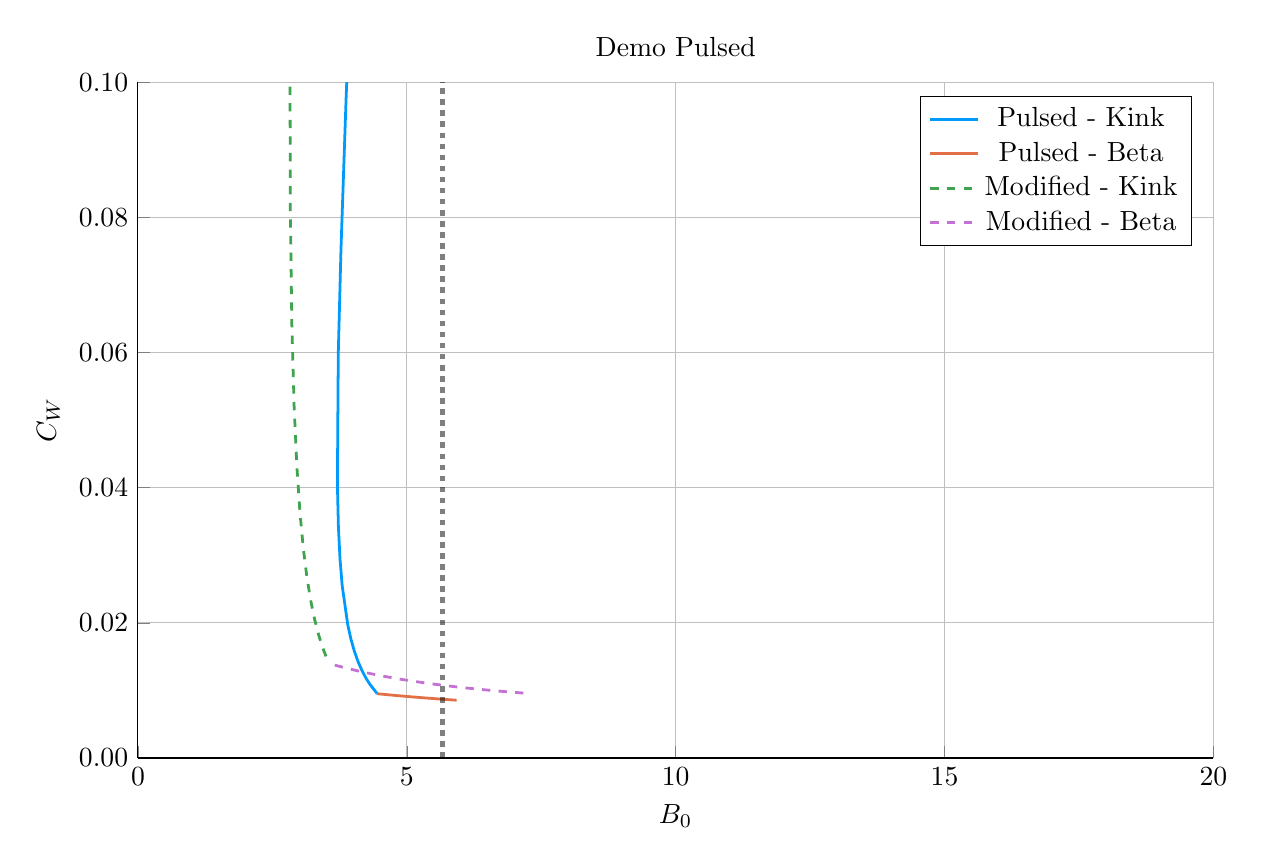
\begin{tikzpicture}[]
\begin{axis}[height = {101.6mm}, ylabel = {${C}_{W}$}, title = {Demo Pulsed}, xmin = {0.0}, xmax = {20.0}, ymax = {0.1}, xlabel = {${B}_{0}$}, {unbounded coords=jump, scaled x ticks = false, xticklabel style={rotate = 0}, xmajorgrids = true, xtick = {0.0,5.0,10.0,15.0,20.0}, xticklabels = {0,5,10,15,20}, xtick align = inside, axis lines* = left, scaled y ticks = false, yticklabel style={rotate = 0}, ymajorgrids = true, ytick = {0.0,0.02,0.04,0.06,0.08,0.1}, yticklabels = {0.00,0.02,0.04,0.06,0.08,0.10}, ytick align = inside, axis lines* = left,     xshift = 0.0mm,
    yshift = 0.0mm,
    axis background/.style={fill={rgb,1:red,1.00000000;green,1.00000000;blue,1.00000000}}
, colorbar style={title=}}, ymin = {0.0}, width = {152.4mm}]\addplot+ [color = {rgb,1:red,0.00000000;green,0.60560316;blue,0.97868012},
draw opacity=1.0,
line width=1,
solid,mark = none,
mark size = 2.0,
mark options = {
    color = {rgb,1:red,0.00000000;green,0.00000000;blue,0.00000000}, draw opacity = 1.0,
    fill = {rgb,1:red,0.00000000;green,0.60560316;blue,0.97868012}, fill opacity = 1.0,
    line width = 1,
    rotate = 0,
    solid
}]coordinates {
(4.327031075670194, 0.1892287825513326)
(4.038214026054326, 0.13206162052102163)
(3.8713719163129245, 0.09770836377510679)
(3.7758613845615545, 0.0753228145367537)
(3.7257856761317214, 0.05989044017674145)
(3.7090473695925437, 0.04055229837333577)
(3.727711597554826, 0.03426367140819575)
(3.7586131667481433, 0.029359319233913946)
(3.799052518631718, 0.025462690957960717)
(3.901290136389271, 0.019741499311841708)
(3.960577465316514, 0.017607284508542168)
(4.0241209645210345, 0.015819330878112364)
(4.0912717805663785, 0.014306863958145555)
(4.161514602943343, 0.013016229386127556)
(4.2344343960723005, 0.0119061698584303)
(4.309692554546368, 0.010944552619225426)
(4.450417240491067, 0.009508186007059894)
};
\addlegendentry{Pulsed - Kink}
\addplot+ [color = {rgb,1:red,0.88887350;green,0.43564919;blue,0.27812294},
draw opacity=1.0,
line width=1,
solid,mark = none,
mark size = 2.0,
mark options = {
    color = {rgb,1:red,0.00000000;green,0.00000000;blue,0.00000000}, draw opacity = 1.0,
    fill = {rgb,1:red,0.88887350;green,0.43564919;blue,0.27812294}, fill opacity = 1.0,
    line width = 1,
    rotate = 0,
    solid
}]coordinates {
(4.450417240491067, 0.009508186007059894)
(4.490148631384312, 0.009477474217304566)
(4.692490181445514, 0.009325449924582748)
(4.8960344619053355, 0.009179881556836224)
(5.100651132702229, 0.00904086745514222)
(5.306202822090688, 0.008908420253381469)
(5.512545696627038, 0.008782491226353)
(5.719530043226767, 0.008662988371093566)
(5.927000883375481, 0.00854978980550123)
};
\addlegendentry{Pulsed - Beta}
\addplot+ [color = {rgb,1:red,0.24222430;green,0.64327509;blue,0.30444865},
draw opacity=1.0,
line width=1,
dashed,mark = none,
mark size = 2.0,
mark options = {
    color = {rgb,1:red,0.00000000;green,0.00000000;blue,0.00000000}, draw opacity = 1.0,
    fill = {rgb,1:red,0.24222430;green,0.64327509;blue,0.30444865}, fill opacity = 1.0,
    line width = 1,
    rotate = 0,
    solid
}]coordinates {
(3.4087424183072135, 0.34025279914240075)
(2.977074181068944, 0.20266043375242454)
(2.8592500074202523, 0.14107963570535767)
(2.827199220063259, 0.10460917631328934)
(2.8339789008667826, 0.08069963800921795)
(2.862412302880871, 0.06408640910554732)
(2.9044598258085443, 0.05207050885933721)
(2.95577893007882, 0.04311069749575431)
(3.0137895352525907, 0.03626387631819784)
(3.076849710218805, 0.03092374739004359)
(3.1438583711612704, 0.02668548743841045)
(3.214045733980633, 0.023270423882766844)
(3.2868548955983727, 0.020481784288090023)
(3.361871149981842, 0.018177576354657807)
(3.4387778750377818, 0.016253383634250513)
(3.5173279629378453, 0.014631131503744007)
};
\addlegendentry{Modified - Kink}
\addplot+ [color = {rgb,1:red,0.76444018;green,0.44411178;blue,0.82429754},
draw opacity=1.0,
line width=1,
dashed,mark = none,
mark size = 2.0,
mark options = {
    color = {rgb,1:red,0.00000000;green,0.00000000;blue,0.00000000}, draw opacity = 1.0,
    fill = {rgb,1:red,0.76444018;green,0.44411178;blue,0.82429754}, fill opacity = 1.0,
    line width = 1,
    rotate = 0,
    solid
}]coordinates {
(3.6607028750648505, 0.013744899135556416)
(3.8574448036470477, 0.013332033203155177)
(4.056375867871351, 0.012949491171136135)
(4.257366397480293, 0.012594759179481692)
(4.460279103534801, 0.012265542491796714)
(4.664969389370631, 0.011959760748489753)
(4.871285596007394, 0.011675536110154509)
(5.07906923307514, 0.01141117796484883)
(5.288155233306219, 0.011165166374807946)
(5.498372259673351, 0.010936135522073528)
(5.709543087166185, 0.010722857854384784)
(5.921485076209294, 0.010524229289897682)
(6.134010749367255, 0.010339255636975386)
(6.346928478632384, 0.0101670402635639)
(6.560043285872518, 0.010006772983002756)
(6.773157754368795, 0.009857720087022352)
(6.986073044284746, 0.009719215441404045)
(7.198590001107076, 0.00959065255201969)
};
\addlegendentry{Modified - Beta}
\addplot+ [color = {rgb,1:red,0.00000000;green,0.00000000;blue,0.00000000},
draw opacity=0.5,
line width=2,
dotted,mark = none,
mark size = 2.0,
mark options = {
    color = {rgb,1:red,0.00000000;green,0.00000000;blue,0.00000000}, draw opacity = 0.5,
    fill = {rgb,1:red,0.00000000;green,0.00000000;blue,0.00000000}, fill opacity = 0.5,
    line width = 1,
    rotate = 0,
    solid
},forget plot]coordinates {
(0.0, NaN)
(20.0, NaN)
};
\addplot+ [color = {rgb,1:red,0.00000000;green,0.00000000;blue,0.00000000},
draw opacity=0.5,
line width=2,
dotted,mark = none,
mark size = 2.0,
mark options = {
    color = {rgb,1:red,0.00000000;green,0.00000000;blue,0.00000000}, draw opacity = 0.5,
    fill = {rgb,1:red,0.00000000;green,0.00000000;blue,0.00000000}, fill opacity = 0.5,
    line width = 1,
    rotate = 0,
    solid
},forget plot]coordinates {
(5.667, 0.0)
(5.667, 0.1)
};
\addplot+[draw=none, color = {rgb,1:red,0.00000000;green,0.00000000;blue,0.00000000},
draw opacity=0.5,
line width=0,
solid,mark = *,
mark size = 2.0,
mark options = {
    color = {rgb,1:red,0.00000000;green,0.00000000;blue,0.00000000}, draw opacity = 0.5,
    fill = {rgb,1:red,0.00000000;green,0.00000000;blue,0.00000000}, fill opacity = 0.5,
    line width = 1,
    rotate = 0,
    solid
},forget plot] coordinates {
(5.667, NaN)
};
\end{axis}

\end{tikzpicture}

		\end{adjustbox}
        \caption{Demo Pulsed Cost-per-Watt}
    \end{subfigure}
    \hfill
    \begin{subfigure}[t]{0.45\textwidth}
        \centering
		\begin{adjustbox}{width=\textwidth}
			\Large
			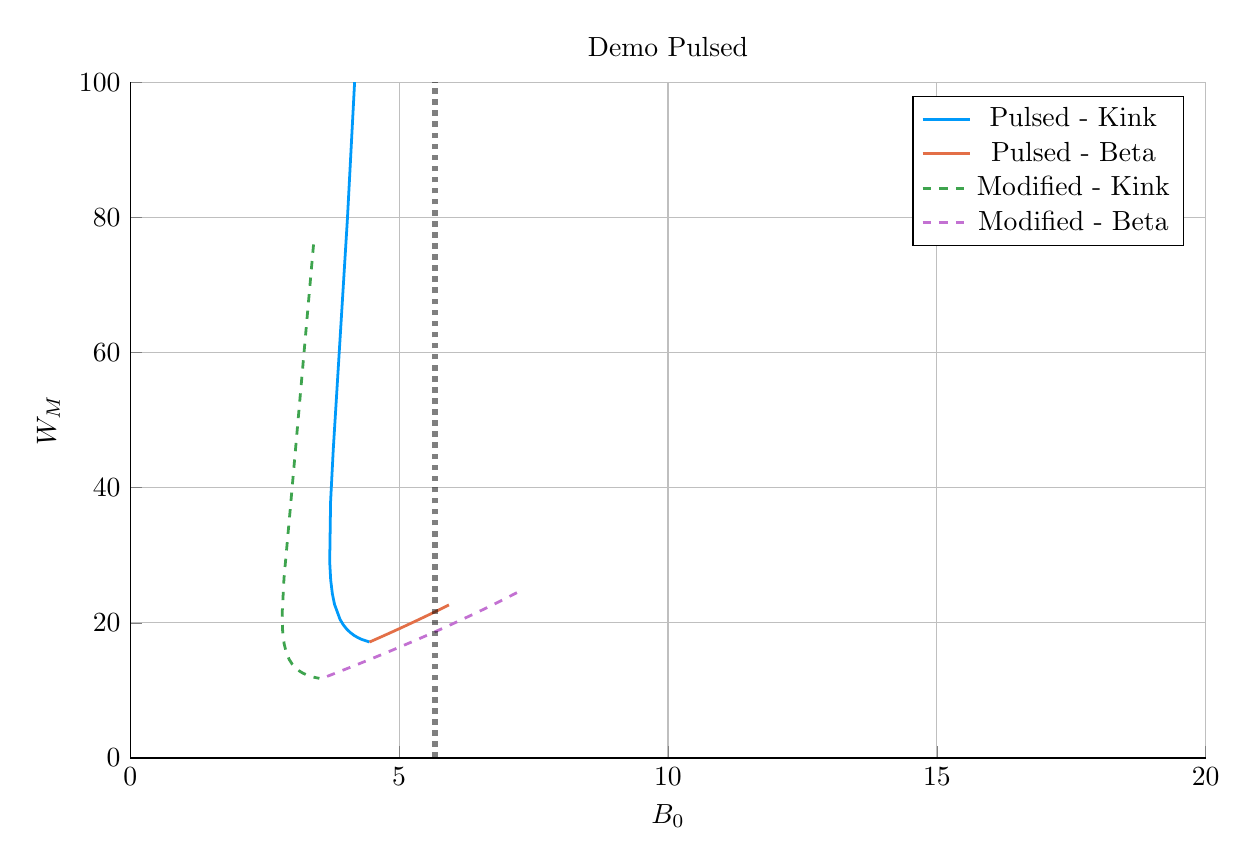
\begin{tikzpicture}[]
\begin{axis}[height = {101.6mm}, ylabel = {${W}_{M}$}, title = {Demo Pulsed}, xmin = {0.0}, xmax = {20.0}, ymax = {100.0}, xlabel = {${B}_{0}$}, {unbounded coords=jump, scaled x ticks = false, xticklabel style={rotate = 0}, xmajorgrids = true, xtick = {0.0,5.0,10.0,15.0,20.0}, xticklabels = {0,5,10,15,20}, xtick align = inside, axis lines* = left, scaled y ticks = false, yticklabel style={rotate = 0}, ymajorgrids = true, ytick = {0.0,20.0,40.0,60.0,80.0,100.0}, yticklabels = {0,20,40,60,80,100}, ytick align = inside, axis lines* = left,     xshift = 0.0mm,
    yshift = 0.0mm,
    axis background/.style={fill={rgb,1:red,1.00000000;green,1.00000000;blue,1.00000000}}
, colorbar style={title=}}, ymin = {0.0}, width = {152.4mm}]\addplot+ [color = {rgb,1:red,0.00000000;green,0.60560316;blue,0.97868012},
draw opacity=1.0,
line width=1,
solid,mark = none,
mark size = 2.0,
mark options = {
    color = {rgb,1:red,0.00000000;green,0.00000000;blue,0.00000000}, draw opacity = 1.0,
    fill = {rgb,1:red,0.00000000;green,0.60560316;blue,0.97868012}, fill opacity = 1.0,
    line width = 1,
    rotate = 0,
    solid
}]coordinates {
(4.327031075670194, 123.44373673332173)
(4.038214026054326, 79.76523284023226)
(3.8713719163129245, 58.108897430981536)
(3.7758613845615545, 45.733304605517155)
(3.7257856761317214, 37.95828264093558)
(3.7090473695925437, 29.04694896379975)
(3.727711597554826, 26.344517979953586)
(3.7586131667481433, 24.306117941226923)
(3.799052518631718, 22.733747168495924)
(3.901290136389271, 20.517766605492294)
(3.960577465316514, 19.728940193613518)
(4.0241209645210345, 19.090733790490855)
(4.0912717805663785, 18.572256162198553)
(4.161514602943343, 18.150497380470465)
(4.2344343960723005, 17.808002600991745)
(4.309692554546368, 17.531315861496644)
(4.450417240491067, 17.166473566094577)
};
\addlegendentry{Pulsed - Kink}
\addplot+ [color = {rgb,1:red,0.88887350;green,0.43564919;blue,0.27812294},
draw opacity=1.0,
line width=1,
solid,mark = none,
mark size = 2.0,
mark options = {
    color = {rgb,1:red,0.00000000;green,0.00000000;blue,0.00000000}, draw opacity = 1.0,
    fill = {rgb,1:red,0.88887350;green,0.43564919;blue,0.27812294}, fill opacity = 1.0,
    line width = 1,
    rotate = 0,
    solid
}]coordinates {
(4.450417240491067, 17.166473566094577)
(4.490148631384312, 17.305309015848636)
(4.692490181445514, 18.019389484737392)
(4.8960344619053355, 18.749800407200777)
(5.100651132702229, 19.496700146051747)
(5.306202822090688, 20.26030213940914)
(5.512545696627038, 21.04087102241869)
(5.719530043226767, 21.83871936060431)
(5.927000883375481, 22.654204785704835)
};
\addlegendentry{Pulsed - Beta}
\addplot+ [color = {rgb,1:red,0.24222430;green,0.64327509;blue,0.30444865},
draw opacity=1.0,
line width=1,
dashed,mark = none,
mark size = 2.0,
mark options = {
    color = {rgb,1:red,0.00000000;green,0.00000000;blue,0.00000000}, draw opacity = 1.0,
    fill = {rgb,1:red,0.24222430;green,0.64327509;blue,0.30444865}, fill opacity = 1.0,
    line width = 1,
    rotate = 0,
    solid
}]coordinates {
(3.4087424183072135, 76.02109466923234)
(2.977074181068944, 36.99469776498375)
(2.8592500074202523, 26.602664601337402)
(2.827199220063259, 21.660862067495565)
(2.8339789008667826, 18.765953821795108)
(2.862412302880871, 16.874407011263102)
(2.9044598258085443, 15.553537101768894)
(2.95577893007882, 14.590024878457532)
(3.0137895352525907, 13.865991589551562)
(3.076849710218805, 13.310773511983673)
(3.1438583711612704, 12.879335564625128)
(3.214045733980633, 12.54157019826116)
(3.2868548955983727, 12.276561049231674)
(3.361871149981842, 12.069311294803374)
(3.4387778750377818, 11.90878112839417)
(3.5173279629378453, 11.786660090388734)
};
\addlegendentry{Modified - Kink}
\addplot+ [color = {rgb,1:red,0.76444018;green,0.44411178;blue,0.82429754},
draw opacity=1.0,
line width=1,
dashed,mark = none,
mark size = 2.0,
mark options = {
    color = {rgb,1:red,0.00000000;green,0.00000000;blue,0.00000000}, draw opacity = 1.0,
    fill = {rgb,1:red,0.76444018;green,0.44411178;blue,0.82429754}, fill opacity = 1.0,
    line width = 1,
    rotate = 0,
    solid
}]coordinates {
(3.6607028750648505, 12.074397140834275)
(3.8574448036470477, 12.685277919648211)
(4.056375867871351, 13.310146449544076)
(4.257366397480293, 13.949057026240864)
(4.460279103534801, 14.602113733589642)
(4.664969389370631, 15.269467629207359)
(4.871285596007394, 15.951314711845848)
(5.07906923307514, 16.647894398080105)
(5.288155233306219, 17.359488308762714)
(5.498372259673351, 18.086419214151615)
(5.709543087166185, 18.82905002156669)
(5.921485076209294, 19.587782712469505)
(6.134010749367255, 20.363057156601585)
(6.346928478632384, 21.155349745799302)
(6.560043285872518, 21.965171804607706)
(6.773157754368795, 22.79306774804729)
(6.986073044284746, 23.639612971086876)
(7.198590001107076, 24.50541146426436)
};
\addlegendentry{Modified - Beta}
\addplot+ [color = {rgb,1:red,0.00000000;green,0.00000000;blue,0.00000000},
draw opacity=0.5,
line width=2,
dotted,mark = none,
mark size = 2.0,
mark options = {
    color = {rgb,1:red,0.00000000;green,0.00000000;blue,0.00000000}, draw opacity = 0.5,
    fill = {rgb,1:red,0.00000000;green,0.00000000;blue,0.00000000}, fill opacity = 0.5,
    line width = 1,
    rotate = 0,
    solid
},forget plot]coordinates {
(0.0, NaN)
(20.0, NaN)
};
\addplot+ [color = {rgb,1:red,0.00000000;green,0.00000000;blue,0.00000000},
draw opacity=0.5,
line width=2,
dotted,mark = none,
mark size = 2.0,
mark options = {
    color = {rgb,1:red,0.00000000;green,0.00000000;blue,0.00000000}, draw opacity = 0.5,
    fill = {rgb,1:red,0.00000000;green,0.00000000;blue,0.00000000}, fill opacity = 0.5,
    line width = 1,
    rotate = 0,
    solid
},forget plot]coordinates {
(5.667, 0.0)
(5.667, 100.0)
};
\addplot+[draw=none, color = {rgb,1:red,0.00000000;green,0.00000000;blue,0.00000000},
draw opacity=0.5,
line width=0,
solid,mark = *,
mark size = 2.0,
mark options = {
    color = {rgb,1:red,0.00000000;green,0.00000000;blue,0.00000000}, draw opacity = 0.5,
    fill = {rgb,1:red,0.00000000;green,0.00000000;blue,0.00000000}, fill opacity = 0.5,
    line width = 1,
    rotate = 0,
    solid
},forget plot] coordinates {
(5.667, NaN)
};
\end{axis}

\end{tikzpicture}

		\end{adjustbox}
        \caption{Demo Pulsed Capital Cost}
    \end{subfigure}	
    \hfill \hfill ~\\ ~\\ ~\\
    \caption{Pulsed Cost Curves}
    \label{fig:pulsed_costs}
\end{figure*}

Summarizing the conclusions of this subsection, the beta limit is usually the best constraint to operate at. For lowering the cost-per-watt, a reactor should always be run at the highest magnetic field strength ($B_0$) that satisfies the beta limit. This most often occurs when wall loading takes over (for steady-state reactors) or reactors start being physically unrealizable (for pulsed ones). Building cheap to build reactors -- i.e. minimizing capital cost -- then actually proved to make pulsed design one of trade-offs. This is because the beta-kink curve intersection produces a low capital cost reactor, but at the price of operating at a subpar cost-per-watt. Designers should therefore balance the two cost metrics.

\subsection{Utilizing High Field Magnets}

The main conclusion for this paper is that high field magnets are the way to go to build an efficient, compact fusion reactor. In line with the MIT ARC effort, these high fields will be built with high-temperature superconducting (HTS) tape. This innovation is set to double the strength of conventional magnets. The real question is how best to use this technology.

At a very simple level, there are two main places strong magnets can be employed: the toroidal fields ($B_0$) and the central solenoid ($B_{CS}$). The easier mode of operation to start with is steady-state. This is because steady-state tokamaks do not rely on a central solenoid for the profitability of their machines. Further, the cost curves in \cref{fig:steady_cost} show that all these designs would benefit from toroidal fields ($B_0$) not achievable with conventional magnets -- which can only reach around 10 T on a good day.

The more interesting result is that pulsed reactors gain no real benefit from using HTS toroidal field magnets. Within the modern paradigm (i.e. D-T fuel, H-Mode, etc), pulsed reactors never have to exceed the limits of \replaced{less expensive LTS magnets.}{inexpensive, copper magnets.} The place HTS can really help is with the central solenoid, which governs how long a pulse can last. Further, the effect of improving the central solenoid saturates within the range accessible to HTS tape. Again, HTS would be more than adequate for the modern paradigm. These conclusions are shown in \cref{fig:pulsed_sensitivities,fig:pulsed_samplings}.

\begin{figure*}
    \centering
    \hfill 
    \begin{subfigure}[t]{0.45\textwidth}
        \centering
		\begin{adjustbox}{width=\textwidth}
			\Large
			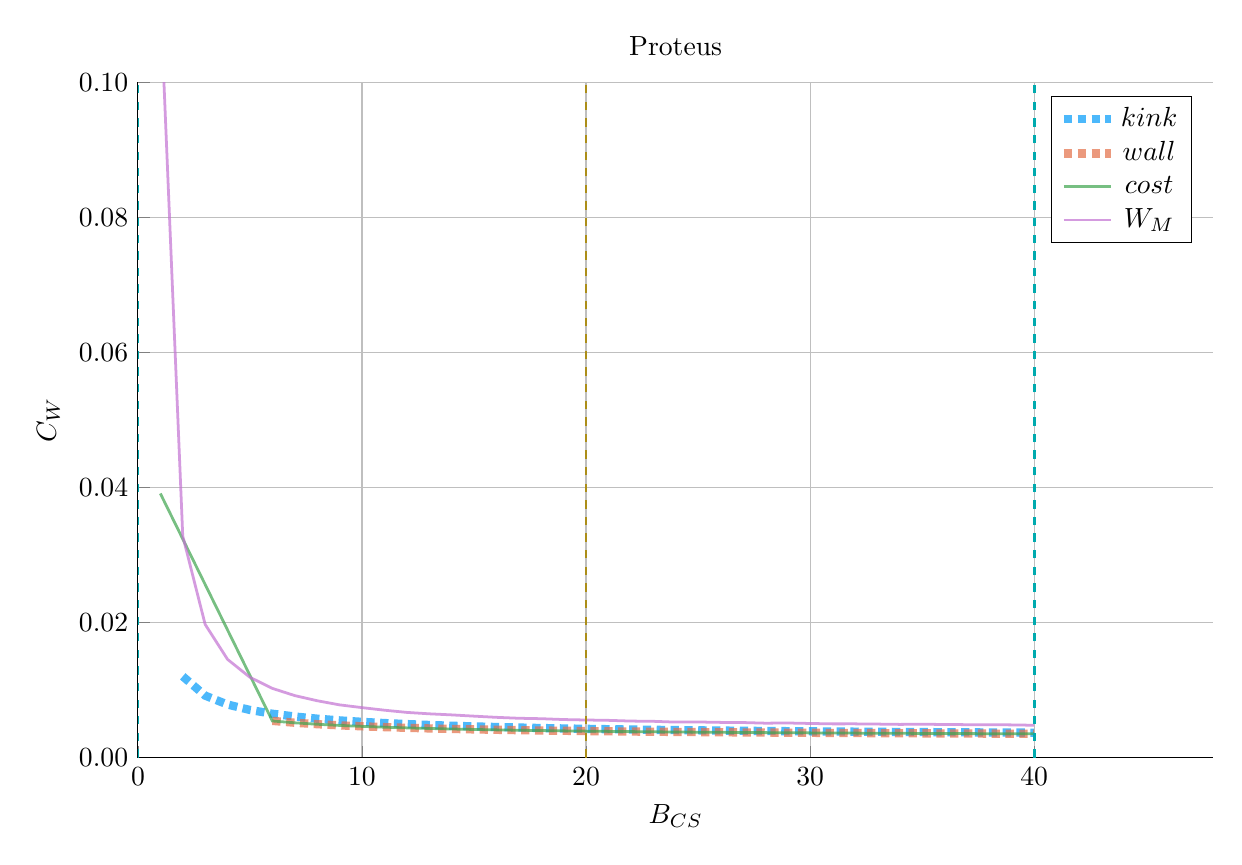
\begin{tikzpicture}[]
\begin{axis}[height = {101.6mm}, ylabel = {${C}_{W}$}, title = {Proteus}, xmin = {0.0}, xmax = {48.0}, ymax = {0.1}, xlabel = {${B}_{CS}$}, {unbounded coords=jump, scaled x ticks = false, xticklabel style={rotate = 0}, xmajorgrids = true, xtick = {0.0,10.0,20.0,30.0,40.0}, xticklabels = {0,10,20,30,40}, xtick align = inside, axis lines* = left, scaled y ticks = false, yticklabel style={rotate = 0}, ymajorgrids = true, ytick = {0.0,0.02,0.04,0.06,0.08,0.1}, yticklabels = {0.00,0.02,0.04,0.06,0.08,0.10}, ytick align = inside, axis lines* = left,     xshift = 0.0mm,
    yshift = 0.0mm,
    axis background/.style={fill={rgb,1:red,1.00000000;green,1.00000000;blue,1.00000000}}
, colorbar style={title=}}, ymin = {0.0}, width = {152.4mm}]\addplot+ [color = {rgb,1:red,0.00000000;green,0.60560316;blue,0.97868012},
draw opacity=0.7,
line width=3,
dotted,mark = none,
mark size = 2.0,
mark options = {
    color = {rgb,1:red,0.00000000;green,0.00000000;blue,0.00000000}, draw opacity = 0.7,
    fill = {rgb,1:red,0.00000000;green,0.60560316;blue,0.97868012}, fill opacity = 0.7,
    line width = 1,
    rotate = 0,
    solid
}]coordinates {
(2.0, 0.01203588028473762)
(3.0, 0.009184398565447248)
(4.0, 0.007862884013421416)
(5.0, 0.007057989599185806)
(6.0, 0.006502613319842857)
(7.0, 0.006090672614199328)
(8.0, 0.005770350019203115)
(9.0, 0.005512859892710094)
(10.0, 0.005300727695239639)
(11.0, 0.005122630604633569)
(12.0, 0.004970854616305319)
(13.0, 0.00483993073972795)
(14.0, 0.0047258536533321)
(15.0, 0.004625609812173743)
(16.0, 0.004536878856245803)
(17.0, 0.004457840030041975)
(18.0, 0.004387039347241793)
(19.0, 0.004323297793305687)
(20.0, 0.004265648725148842)
(21.0, 0.00421328852908289)
(22.0, 0.004165543387382086)
(23.0, 0.0041218418382133306)
(24.0, 0.004081697424729452)
(25.0, 0.004044691025187507)
(26.0, 0.004010460170934446)
(27.0, 0.00397868942182741)
(28.0, 0.003949102890414613)
(29.0, 0.003921458228696752)
(30.0, 0.0038955417483358588)
(31.0, 0.00387116442730114)
(32.0, 0.003848158715413871)
(33.0, 0.0038263753834889853)
(34.0, 0.003805681791784416)
(35.0, 0.0037859598267780737)
(36.0, 0.003767103936991627)
(37.0, 0.003749019788626583)
(38.0, 0.0037316235037579658)
(39.0, 0.0037148400629903496)
(40.0, 0.003698602652227772)
};
\addlegendentry{$kink$}
\addplot+ [color = {rgb,1:red,0.88887350;green,0.43564919;blue,0.27812294},
draw opacity=0.7,
line width=3,
dotted,mark = none,
mark size = 2.0,
mark options = {
    color = {rgb,1:red,0.00000000;green,0.00000000;blue,0.00000000}, draw opacity = 0.7,
    fill = {rgb,1:red,0.88887350;green,0.43564919;blue,0.27812294}, fill opacity = 0.7,
    line width = 1,
    rotate = 0,
    solid
}]coordinates {
(6.0, 0.0054444534313977866)
(7.0, 0.005168634641274746)
(8.0, 0.004954271193511655)
(9.0, 0.004781774855931542)
(10.0, 0.0046393940524333595)
(11.0, 0.004519572327657892)
(12.0, 0.004417187891782309)
(13.0, 0.004328621916738755)
(14.0, 0.004251229863078844)
(15.0, 0.004183024392188461)
(16.0, 0.004122476375660697)
(17.0, 0.004068385219748399)
(18.0, 0.004019791621043741)
(19.0, 0.003975917241919141)
(20.0, 0.003936121998618529)
(21.0, 0.0038998731854890116)
(22.0, 0.0038667227426346573)
(23.0, 0.0038362902440819057)
(24.0, 0.003808249979473852)
(25.0, 0.003782321013899768)
(26.0, 0.003758259446775421)
(27.0, 0.003735852316365348)
(28.0, 0.0037149127505960292)
(29.0, 0.0036952760721994664)
(30.0, 0.003676796641638663)
(31.0, 0.003659345275564596)
(32.0, 0.003642807117806076)
(33.0, 0.0036270798687725717)
(34.0, 0.003612072300608303)
(35.0, 0.0035977030015636596)
(36.0, 0.0035838993052924165)
(37.0, 0.003570596370170802)
(38.0, 0.0035577363809944163)
(39.0, 0.003545267851071995)
(40.0, 0.003533145007184075)
};
\addlegendentry{$wall$}
\addplot+ [color = {rgb,1:red,0.24222430;green,0.64327509;blue,0.30444865},
draw opacity=0.7,
line width=1,
solid,mark = none,
mark size = 2.0,
mark options = {
    color = {rgb,1:red,0.00000000;green,0.00000000;blue,0.00000000}, draw opacity = 0.7,
    fill = {rgb,1:red,0.24222430;green,0.64327509;blue,0.30444865}, fill opacity = 0.7,
    line width = 1,
    rotate = 0,
    solid
}]coordinates {
(1.0, 0.03911143879274214)
(6.0, 0.005431918985170686)
(7.0, 0.005156651927896806)
(8.0, 0.0049427222925668)
(9.0, 0.004770577307210836)
(10.0, 0.004628487505103093)
(11.0, 0.004508911021409933)
(12.0, 0.004406736153465557)
(13.0, 0.004318351239259131)
(14.0, 0.0042411171388798095)
(15.0, 0.004173050519899446)
(16.0, 0.00411262543808849)
(17.0, 0.0040586437812760905)
(18.0, 0.004010148222137883)
(19.0, 0.003966362101140297)
(20.0, 0.003926646631736614)
(21.0, 0.003890470261769361)
(22.0, 0.003857385855340664)
(23.0, 0.003827013846123357)
(24.0, 0.003799029152446192)
(25.0, 0.0037731515135378028)
(26.0, 0.0037491374742800476)
(27.0, 0.003726774572373303)
(28.0, 0.0037058763309042774)
(29.0, 0.0036862784148944654)
(30.0, 0.0036678355176402353)
(31.0, 0.0036504187072176437)
(32.0, 0.0036339133609214515)
(33.0, 0.003618217419267161)
(34.0, 0.003603239855200063)
(35.0, 0.0035888993956205303)
(36.0, 0.003575123536625824)
(37.0, 0.0035618476053302967)
(38.0, 0.00354901385682175)
(39.0, 0.0035365709088021192)
(40.0, 0.0035244731223137145)
};
\addlegendentry{$cost$}
\addplot+ [color = {rgb,1:red,0.76444018;green,0.44411178;blue,0.82429754},
draw opacity=0.7,
line width=1,
solid,mark = none,
mark size = 2.0,
mark options = {
    color = {rgb,1:red,0.00000000;green,0.00000000;blue,0.00000000}, draw opacity = 0.7,
    fill = {rgb,1:red,0.76444018;green,0.44411178;blue,0.82429754}, fill opacity = 0.7,
    line width = 1,
    rotate = 0,
    solid
}]coordinates {
(1.0, 0.11281791824873516)
(2.0, 0.032817502153924004)
(3.0, 0.019728226993225767)
(4.0, 0.014550673387607675)
(5.0, 0.01189537503222638)
(6.0, 0.010254586386818185)
(7.0, 0.009187722848027494)
(8.0, 0.008426409595366063)
(9.0, 0.007814460956383539)
(10.0, 0.007407116893402244)
(11.0, 0.007026609234473925)
(12.0, 0.006699623094822548)
(13.0, 0.006490049586328449)
(14.0, 0.006332285776340749)
(15.0, 0.006145121123500574)
(16.0, 0.005968637732544897)
(17.0, 0.005831116183284295)
(18.0, 0.005766436928694199)
(19.0, 0.005641758652539625)
(20.0, 0.005573536740322697)
(21.0, 0.005522757977005573)
(22.0, 0.005416005772196298)
(23.0, 0.005379655600977924)
(24.0, 0.005261536268439173)
(25.0, 0.005281022329992938)
(26.0, 0.0052218684208626695)
(27.0, 0.005199327855049588)
(28.0, 0.005104248642193906)
(29.0, 0.005130959429711627)
(30.0, 0.005061392939220031)
(31.0, 0.005001395595923804)
(32.0, 0.005003038146366862)
(33.0, 0.004969709625977857)
(34.0, 0.004924506782614121)
(35.0, 0.004946663939864212)
(36.0, 0.004912455965902953)
(37.0, 0.004883749116586274)
(38.0, 0.004871307710986148)
(39.0, 0.004851151446945242)
(40.0, 0.004795575554984452)
};
\addlegendentry{$W_M$}
\addplot+ [color = {rgb,1:red,0.67554396;green,0.55566233;blue,0.09423434},
draw opacity=1.0,
line width=1,
dashed,mark = none,
mark size = 2.0,
mark options = {
    color = {rgb,1:red,0.00000000;green,0.00000000;blue,0.00000000}, draw opacity = 1.0,
    fill = {rgb,1:red,0.67554396;green,0.55566233;blue,0.09423434}, fill opacity = 1.0,
    line width = 1,
    rotate = 0,
    solid
},forget plot]coordinates {
(20.0, 0.0)
(20.0, 0.1)
};
\addplot+ [color = {rgb,1:red,0.00000048;green,0.66575898;blue,0.68099695},
draw opacity=1.0,
line width=1,
dashed,mark = none,
mark size = 2.0,
mark options = {
    color = {rgb,1:red,0.00000000;green,0.00000000;blue,0.00000000}, draw opacity = 1.0,
    fill = {rgb,1:red,0.00000048;green,0.66575898;blue,0.68099695}, fill opacity = 1.0,
    line width = 1,
    rotate = 0,
    solid
},forget plot]coordinates {
(0.0, 0.0)
(0.0, 0.1)
};
\addplot+ [color = {rgb,1:red,0.00000048;green,0.66575898;blue,0.68099695},
draw opacity=1.0,
line width=1,
dashed,mark = none,
mark size = 2.0,
mark options = {
    color = {rgb,1:red,0.00000000;green,0.00000000;blue,0.00000000}, draw opacity = 1.0,
    fill = {rgb,1:red,0.00000048;green,0.66575898;blue,0.68099695}, fill opacity = 1.0,
    line width = 1,
    rotate = 0,
    solid
},forget plot]coordinates {
(40.0, 0.0)
(40.0, 0.1)
};
\end{axis}

\end{tikzpicture}

		\end{adjustbox}
        \caption{Proteus Cost-per-Watt}
    \end{subfigure}
    \hfill
    \begin{subfigure}[t]{0.45\textwidth}
        \centering
		\begin{adjustbox}{width=\textwidth}
			\Large
			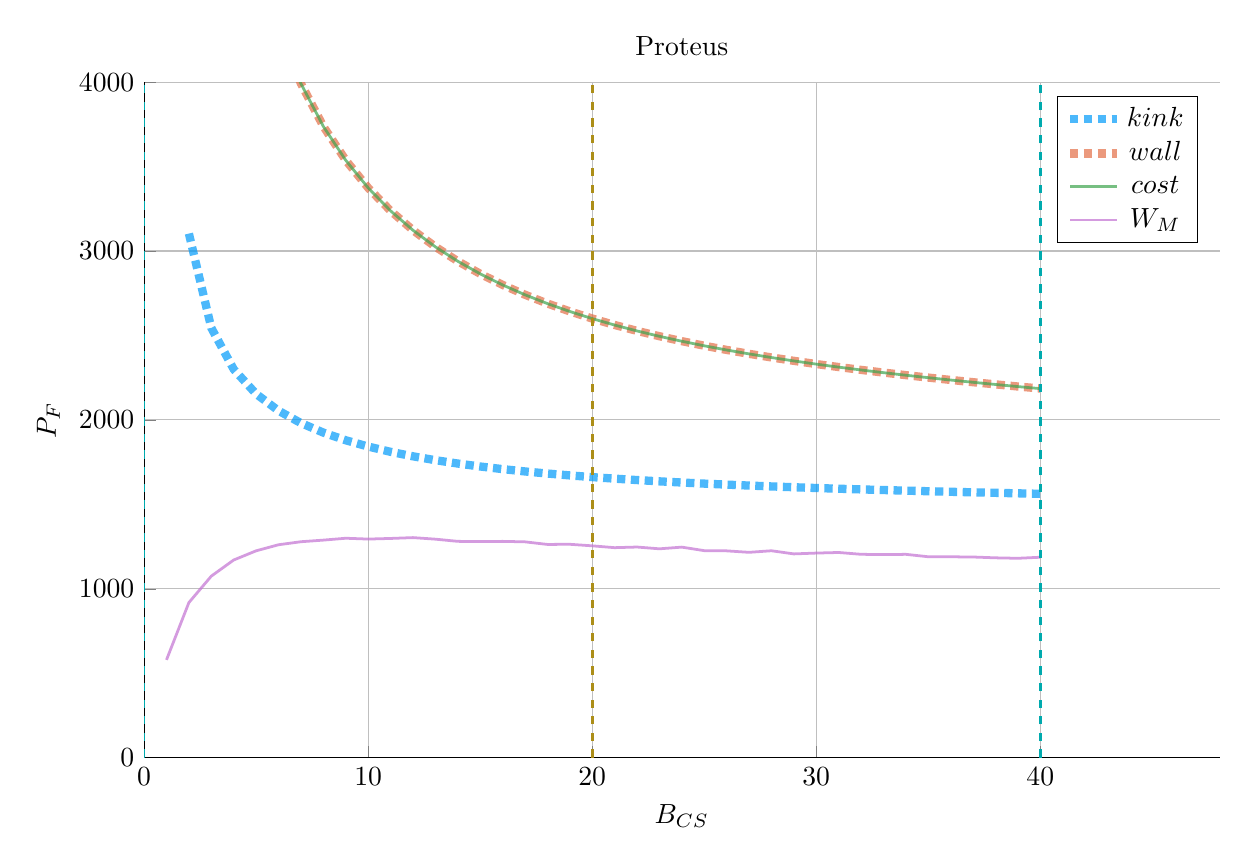
\begin{tikzpicture}[]
\begin{axis}[height = {101.6mm}, ylabel = {${P}_{F}$}, title = {Proteus}, xmin = {0.0}, xmax = {48.0}, ymax = {4000.0}, xlabel = {${B}_{CS}$}, {unbounded coords=jump, scaled x ticks = false, xticklabel style={rotate = 0}, xmajorgrids = true, xtick = {0.0,10.0,20.0,30.0,40.0}, xticklabels = {0,10,20,30,40}, xtick align = inside, axis lines* = left, scaled y ticks = false, yticklabel style={rotate = 0}, ymajorgrids = true, ytick = {0.0,1000.0,2000.0,3000.0,4000.0}, yticklabels = {0,1000,2000,3000,4000}, ytick align = inside, axis lines* = left,     xshift = 0.0mm,
    yshift = 0.0mm,
    axis background/.style={fill={rgb,1:red,1.00000000;green,1.00000000;blue,1.00000000}}
, colorbar style={title=}}, ymin = {0.0}, width = {152.4mm}]\addplot+ [color = {rgb,1:red,0.00000000;green,0.60560316;blue,0.97868012},
draw opacity=0.7,
line width=3,
dotted,mark = none,
mark size = 2.0,
mark options = {
    color = {rgb,1:red,0.00000000;green,0.00000000;blue,0.00000000}, draw opacity = 0.7,
    fill = {rgb,1:red,0.00000000;green,0.60560316;blue,0.97868012}, fill opacity = 0.7,
    line width = 1,
    rotate = 0,
    solid
}]coordinates {
(2.0, 3103.446964483028)
(3.0, 2544.8446560898697)
(4.0, 2299.7883505862683)
(5.0, 2153.9401008014215)
(6.0, 2054.566085735622)
(7.0, 1981.4265807089412)
(8.0, 1924.8436783738584)
(9.0, 1879.5196356674505)
(10.0, 1842.2729246450338)
(11.0, 1811.058926720514)
(12.0, 1784.4936387453804)
(13.0, 1761.6008925896194)
(14.0, 1741.6687589347825)
(15.0, 1724.1634290251588)
(16.0, 1708.675049552884)
(17.0, 1694.8827715321645)
(18.0, 1682.530881991843)
(19.0, 1671.41236950268)
(20.0, 1661.3577430103219)
(21.0, 1652.2262595201232)
(22.0, 1643.9000207526378)
(23.0, 1636.2791174294293)
(24.0, 1629.2785569006053)
(25.0, 1622.8251506662725)
(26.0, 1616.8556306952612)
(27.0, 1611.314956936522)
(28.0, 1606.1550041060862)
(29.0, 1601.3335066156708)
(30.0, 1596.813203261599)
(31.0, 1592.5611379345382)
(32.0, 1588.5481006380803)
(33.0, 1584.7480767592144)
(34.0, 1581.137944358817)
(35.0, 1577.697113913979)
(36.0, 1574.4071855210084)
(37.0, 1571.2517143488374)
(38.0, 1568.2160778261118)
(39.0, 1565.2871970827582)
(40.0, 1562.4534231467098)
};
\addlegendentry{$kink$}
\addplot+ [color = {rgb,1:red,0.88887350;green,0.43564919;blue,0.27812294},
draw opacity=0.7,
line width=3,
dotted,mark = none,
mark size = 2.0,
mark options = {
    color = {rgb,1:red,0.00000000;green,0.00000000;blue,0.00000000}, draw opacity = 0.7,
    fill = {rgb,1:red,0.88887350;green,0.43564919;blue,0.27812294}, fill opacity = 0.7,
    line width = 1,
    rotate = 0,
    solid
}]coordinates {
(6.0, 4323.6250098364)
(7.0, 3991.769889747364)
(8.0, 3738.5019719471065)
(9.0, 3537.844669896544)
(10.0, 3374.4482917260734)
(11.0, 3238.5755547510726)
(12.0, 3123.707522754923)
(13.0, 3025.2906069442192)
(14.0, 2940.0327020869304)
(15.0, 2865.4848852505193)
(16.0, 2799.781119223045)
(17.0, 2741.4699493813873)
(18.0, 2689.4020933235506)
(19.0, 2642.653242662454)
(20.0, 2600.4697515783287)
(21.0, 2562.2296107375905)
(22.0, 2527.4138764273603)
(23.0, 2495.5854037525905)
(24.0, 2466.372779394115)
(25.0, 2439.458018649117)
(26.0, 2414.5670292139203)
(27.0, 2391.4621364565396)
(28.0, 2369.9361636649223)
(29.0, 2349.807698422879)
(30.0, 2330.917272823136)
(31.0, 2313.1242542242217)
(32.0, 2296.3042930448983)
(33.0, 2280.3472105413966)
(34.0, 2265.1552364984454)
(35.0, 2250.64152696625)
(36.0, 2236.728907456072)
(37.0, 2223.34879867789)
(38.0, 2210.440290899089)
(39.0, 2197.9493399942594)
(40.0, 2185.8280637304556)
};
\addlegendentry{$wall$}
\addplot+ [color = {rgb,1:red,0.24222430;green,0.64327509;blue,0.30444865},
draw opacity=0.7,
line width=1,
solid,mark = none,
mark size = 2.0,
mark options = {
    color = {rgb,1:red,0.00000000;green,0.00000000;blue,0.00000000}, draw opacity = 0.7,
    fill = {rgb,1:red,0.24222430;green,0.64327509;blue,0.30444865}, fill opacity = 0.7,
    line width = 1,
    rotate = 0,
    solid
}]coordinates {
(6.0, 4323.626574700694)
(7.0, 3991.6631892643886)
(8.0, 3738.320677711505)
(9.0, 3537.608432111376)
(10.0, 3374.169551170435)
(11.0, 3238.26268518392)
(12.0, 3123.3664382128786)
(13.0, 3024.925648281227)
(14.0, 2939.6471637487452)
(15.0, 2865.0813351410798)
(16.0, 2799.36161050096)
(17.0, 2741.036157991272)
(18.0, 2688.955412764389)
(19.0, 2642.1948546153712)
(20.0, 2600.0006699519377)
(21.0, 2561.750720954071)
(22.0, 2526.9259593565384)
(23.0, 2495.0891597848504)
(24.0, 2465.868837737165)
(25.0, 2438.946956709572)
(26.0, 2414.0493736799453)
(27.0, 2390.9383771738217)
(28.0, 2369.4067567095603)
(29.0, 2349.2730703154293)
(30.0, 2330.3778259957894)
(31.0, 2312.580367156535)
(32.0, 2295.756323266687)
(33.0, 2279.7954985113834)
(34.0, 2264.600106129103)
(35.0, 2250.0832841784704)
(36.0, 2236.1678437242876)
(37.0, 2222.7851932488634)
(38.0, 2209.8744060154622)
(39.0, 2197.3814243621327)
(40.0, 2185.25835564655)
};
\addlegendentry{$cost$}
\addplot+ [color = {rgb,1:red,0.76444018;green,0.44411178;blue,0.82429754},
draw opacity=0.7,
line width=1,
solid,mark = none,
mark size = 2.0,
mark options = {
    color = {rgb,1:red,0.00000000;green,0.00000000;blue,0.00000000}, draw opacity = 0.7,
    fill = {rgb,1:red,0.76444018;green,0.44411178;blue,0.82429754}, fill opacity = 0.7,
    line width = 1,
    rotate = 0,
    solid
}]coordinates {
(1.0, 579.1770635549526)
(2.0, 918.4032254393342)
(3.0, 1074.9224453723655)
(4.0, 1170.511694377957)
(5.0, 1224.8328861528692)
(6.0, 1260.7420812438745)
(7.0, 1278.6558574628261)
(8.0, 1288.1834994000776)
(9.0, 1299.316367656194)
(10.0, 1294.3919774035123)
(11.0, 1298.0825023461)
(12.0, 1303.0515424091216)
(13.0, 1293.865250965231)
(14.0, 1280.9007331366447)
(15.0, 1279.4372391236866)
(16.0, 1280.7616167001067)
(17.0, 1277.9826713878344)
(18.0, 1262.6816701784642)
(19.0, 1263.51658245539)
(20.0, 1254.3696077727395)
(21.0, 1243.4883851017005)
(22.0, 1247.271738332874)
(23.0, 1236.6841019289109)
(24.0, 1246.6992139316376)
(25.0, 1225.840796579752)
(26.0, 1224.5924675745566)
(27.0, 1215.860267902309)
(28.0, 1225.2315346432224)
(29.0, 1206.5608956425033)
(30.0, 1211.487449032281)
(31.0, 1214.9842647989544)
(32.0, 1204.193043008769)
(33.0, 1202.3951421040542)
(34.0, 1204.0095118625998)
(35.0, 1189.6936123071723)
(36.0, 1189.4184409015577)
(37.0, 1188.1807853881828)
(38.0, 1183.3067663347506)
(39.0, 1180.5861451931135)
(40.0, 1186.8241154535017)
};
\addlegendentry{$W_M$}
\addplot+ [color = {rgb,1:red,0.67554396;green,0.55566233;blue,0.09423434},
draw opacity=1.0,
line width=1,
dashed,mark = none,
mark size = 2.0,
mark options = {
    color = {rgb,1:red,0.00000000;green,0.00000000;blue,0.00000000}, draw opacity = 1.0,
    fill = {rgb,1:red,0.67554396;green,0.55566233;blue,0.09423434}, fill opacity = 1.0,
    line width = 1,
    rotate = 0,
    solid
},forget plot]coordinates {
(20.0, 0.0)
(20.0, 4000.0)
};
\addplot+ [color = {rgb,1:red,0.00000048;green,0.66575898;blue,0.68099695},
draw opacity=1.0,
line width=1,
dashed,mark = none,
mark size = 2.0,
mark options = {
    color = {rgb,1:red,0.00000000;green,0.00000000;blue,0.00000000}, draw opacity = 1.0,
    fill = {rgb,1:red,0.00000048;green,0.66575898;blue,0.68099695}, fill opacity = 1.0,
    line width = 1,
    rotate = 0,
    solid
},forget plot]coordinates {
(0.0, 0.0)
(0.0, 4000.0)
};
\addplot+ [color = {rgb,1:red,0.00000048;green,0.66575898;blue,0.68099695},
draw opacity=1.0,
line width=1,
dashed,mark = none,
mark size = 2.0,
mark options = {
    color = {rgb,1:red,0.00000000;green,0.00000000;blue,0.00000000}, draw opacity = 1.0,
    fill = {rgb,1:red,0.00000048;green,0.66575898;blue,0.68099695}, fill opacity = 1.0,
    line width = 1,
    rotate = 0,
    solid
},forget plot]coordinates {
(40.0, 0.0)
(40.0, 4000.0)
};
\end{axis}

\end{tikzpicture}

		\end{adjustbox}
        \caption{Proteus Fusion Power}
    \end{subfigure}
    \hfill \hfill ~\\ ~\\ ~\\ ~\\
    \hfill 
    \begin{subfigure}[t]{0.45\textwidth}
        \centering
		\begin{adjustbox}{width=\textwidth}
			\Large
			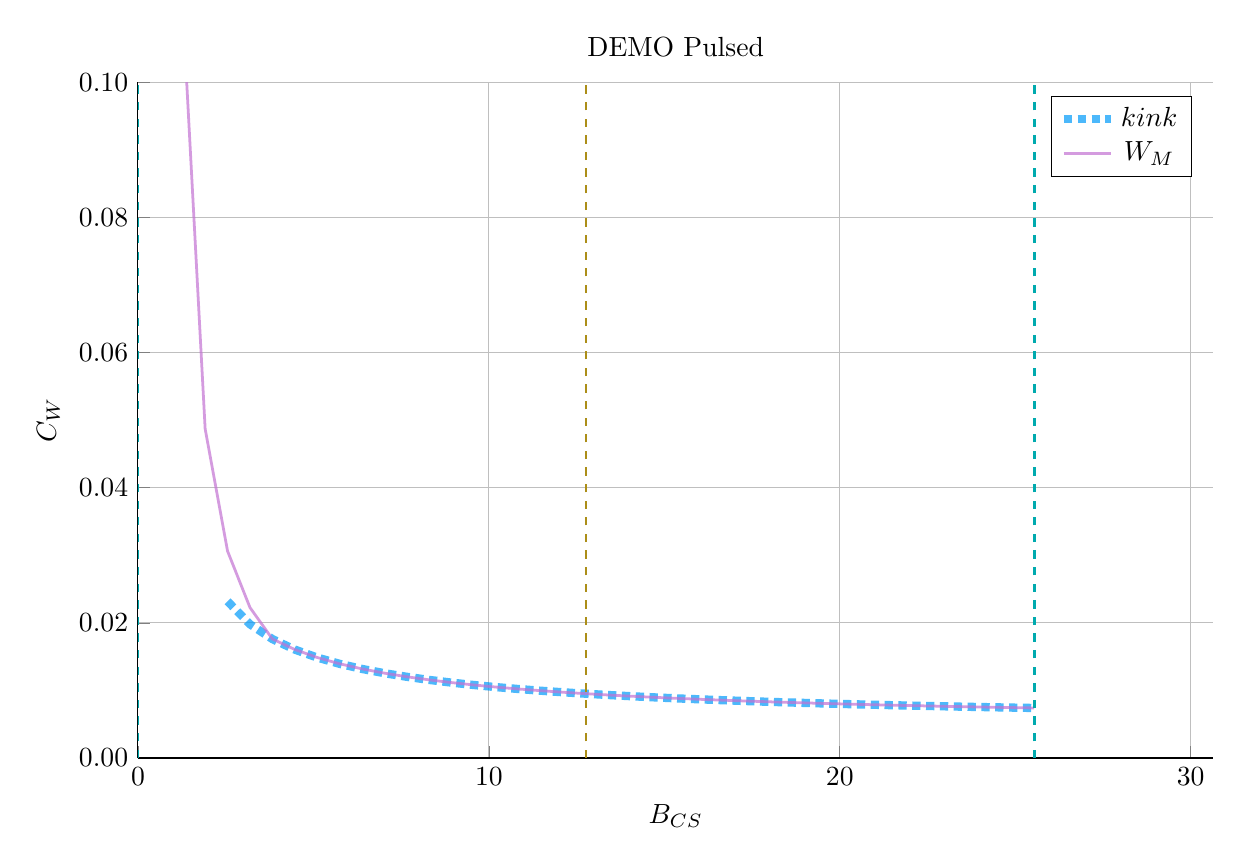
\begin{tikzpicture}[]
\begin{axis}[height = {101.6mm}, ylabel = {${C}_{W}$}, title = {DEMO Pulsed}, xmin = {0.0}, xmax = {30.647999999999996}, ymax = {0.1}, xlabel = {${B}_{CS}$}, {unbounded coords=jump, scaled x ticks = false, xticklabel style={rotate = 0}, xmajorgrids = true, xtick = {0.0,10.0,20.0,30.0}, xticklabels = {0,10,20,30}, xtick align = inside, axis lines* = left, scaled y ticks = false, yticklabel style={rotate = 0}, ymajorgrids = true, ytick = {0.0,0.02,0.04,0.06,0.08,0.1}, yticklabels = {0.00,0.02,0.04,0.06,0.08,0.10}, ytick align = inside, axis lines* = left,     xshift = 0.0mm,
    yshift = 0.0mm,
    axis background/.style={fill={rgb,1:red,1.00000000;green,1.00000000;blue,1.00000000}}
, colorbar style={title=}}, ymin = {0.0}, width = {152.4mm}]\addplot+ [color = {rgb,1:red,0.00000000;green,0.60560316;blue,0.97868012},
draw opacity=0.7,
line width=3,
dotted,mark = none,
mark size = 2.0,
mark options = {
    color = {rgb,1:red,0.00000000;green,0.00000000;blue,0.00000000}, draw opacity = 0.7,
    fill = {rgb,1:red,0.00000000;green,0.60560316;blue,0.97868012}, fill opacity = 0.7,
    line width = 1,
    rotate = 0,
    solid
}]coordinates {
(2.554, 0.02318734520558535)
(3.1925, 0.01979476107899613)
(3.831, 0.017603355037552698)
(4.4695, 0.016044799178348484)
(5.108, 0.014866250639298402)
(5.7465, 0.013936482483239419)
(6.385, 0.01317990783855962)
(7.0235, 0.012549576851985598)
(7.662, 0.012014608821880964)
(8.3005, 0.0115537578450752)
(8.939, 0.011151866449576242)
(9.5775, 0.010797792385662914)
(10.216, 0.01048313680344431)
(10.8545, 0.010201432064429045)
(11.493, 0.009947605124186827)
(12.1315, 0.009717612480587775)
(12.77, 0.009508186007059894)
(13.4085, 0.00931664851451733)
(14.047, 0.0091407869999344)
(14.6855, 0.008978750314220367)
(15.324, 0.008828974406358622)
(15.9625, 0.008690131290406682)
(16.601, 0.00856108205364691)
(17.2395, 0.00844084383977025)
(17.878, 0.008328561855196386)
(18.5165, 0.008223492959290063)
(19.155, 0.008124981083533659)
(19.7935, 0.008032448226206816)
(20.432, 0.00794538294556649)
(21.0705, 0.007863325416792471)
(21.709, 0.007785870780985343)
(22.3475, 0.007712652483079618)
(22.986, 0.007643337657768243)
(23.6245, 0.007577631727123891)
(24.263, 0.007515260912787025)
(24.9015, 0.007455982613051396)
(25.54, 0.0073995698561812534)
};
\addlegendentry{$kink$}
\addplot+ [color = {rgb,1:red,0.76444018;green,0.44411178;blue,0.82429754},
draw opacity=0.7,
line width=1,
solid,mark = none,
mark size = 2.0,
mark options = {
    color = {rgb,1:red,0.00000000;green,0.00000000;blue,0.00000000}, draw opacity = 0.7,
    fill = {rgb,1:red,0.76444018;green,0.44411178;blue,0.82429754}, fill opacity = 0.7,
    line width = 1,
    rotate = 0,
    solid
}]coordinates {
(1.277, 0.11103962259635594)
(1.9155, 0.04872207778751838)
(2.554, 0.030623786781632356)
(3.1925, 0.02227209817598041)
(3.831, 0.017616907013725057)
(4.4695, 0.016056698056099362)
(5.108, 0.014876903024892953)
(5.7465, 0.013946157004488027)
(6.385, 0.013188791795150938)
(7.0235, 0.01255780643010704)
(7.662, 0.012022286474819083)
(8.3005, 0.011560962727119612)
(8.939, 0.011158661188546642)
(9.5775, 0.010804227420746708)
(10.216, 0.010489253514917194)
(10.8545, 0.010207264779534897)
(11.493, 0.009953182722525435)
(12.1315, 0.009722959528177274)
(12.77, 0.00951332304230177)
(13.4085, 0.009321594890974848)
(14.047, 0.009145558054080098)
(14.6855, 0.008983359034690068)
(15.324, 0.008833434022137314)
(15.9625, 0.008694452806924206)
(16.601, 0.008565275282310096)
(17.2395, 0.008444917567257735)
(17.878, 0.008332525241857281)
(18.5165, 0.008227351925267778)
(19.155, 0.008128742121807565)
(19.7935, 0.008036117248420337)
(20.432, 0.007948964229775446)
(21.0705, 0.007866826138305198)
(21.709, 0.007789294347336472)
(22.3475, 0.007716002134627253)
(22.986, 0.007646619130621194)
(23.6245, 0.007580846791208588)
(24.263, 0.007518414534202099)
(24.9015, 0.007459076306986172)
(25.54, 0.00740260787168551)
};
\addlegendentry{$W_M$}
\addplot+ [color = {rgb,1:red,0.67554396;green,0.55566233;blue,0.09423434},
draw opacity=1.0,
line width=1,
dashed,mark = none,
mark size = 2.0,
mark options = {
    color = {rgb,1:red,0.00000000;green,0.00000000;blue,0.00000000}, draw opacity = 1.0,
    fill = {rgb,1:red,0.67554396;green,0.55566233;blue,0.09423434}, fill opacity = 1.0,
    line width = 1,
    rotate = 0,
    solid
},forget plot]coordinates {
(12.77, 0.0)
(12.77, 0.1)
};
\addplot+ [color = {rgb,1:red,0.00000048;green,0.66575898;blue,0.68099695},
draw opacity=1.0,
line width=1,
dashed,mark = none,
mark size = 2.0,
mark options = {
    color = {rgb,1:red,0.00000000;green,0.00000000;blue,0.00000000}, draw opacity = 1.0,
    fill = {rgb,1:red,0.00000048;green,0.66575898;blue,0.68099695}, fill opacity = 1.0,
    line width = 1,
    rotate = 0,
    solid
},forget plot]coordinates {
(0.0, 0.0)
(0.0, 0.1)
};
\addplot+ [color = {rgb,1:red,0.00000048;green,0.66575898;blue,0.68099695},
draw opacity=1.0,
line width=1,
dashed,mark = none,
mark size = 2.0,
mark options = {
    color = {rgb,1:red,0.00000000;green,0.00000000;blue,0.00000000}, draw opacity = 1.0,
    fill = {rgb,1:red,0.00000048;green,0.66575898;blue,0.68099695}, fill opacity = 1.0,
    line width = 1,
    rotate = 0,
    solid
},forget plot]coordinates {
(25.54, 0.0)
(25.54, 0.1)
};
\end{axis}

\end{tikzpicture}

		\end{adjustbox}
        \caption{Demo Pulsed Cost-per-Watt}
    \end{subfigure}
    \hfill
    \begin{subfigure}[t]{0.45\textwidth}
        \centering
		\begin{adjustbox}{width=\textwidth}
			\Large
			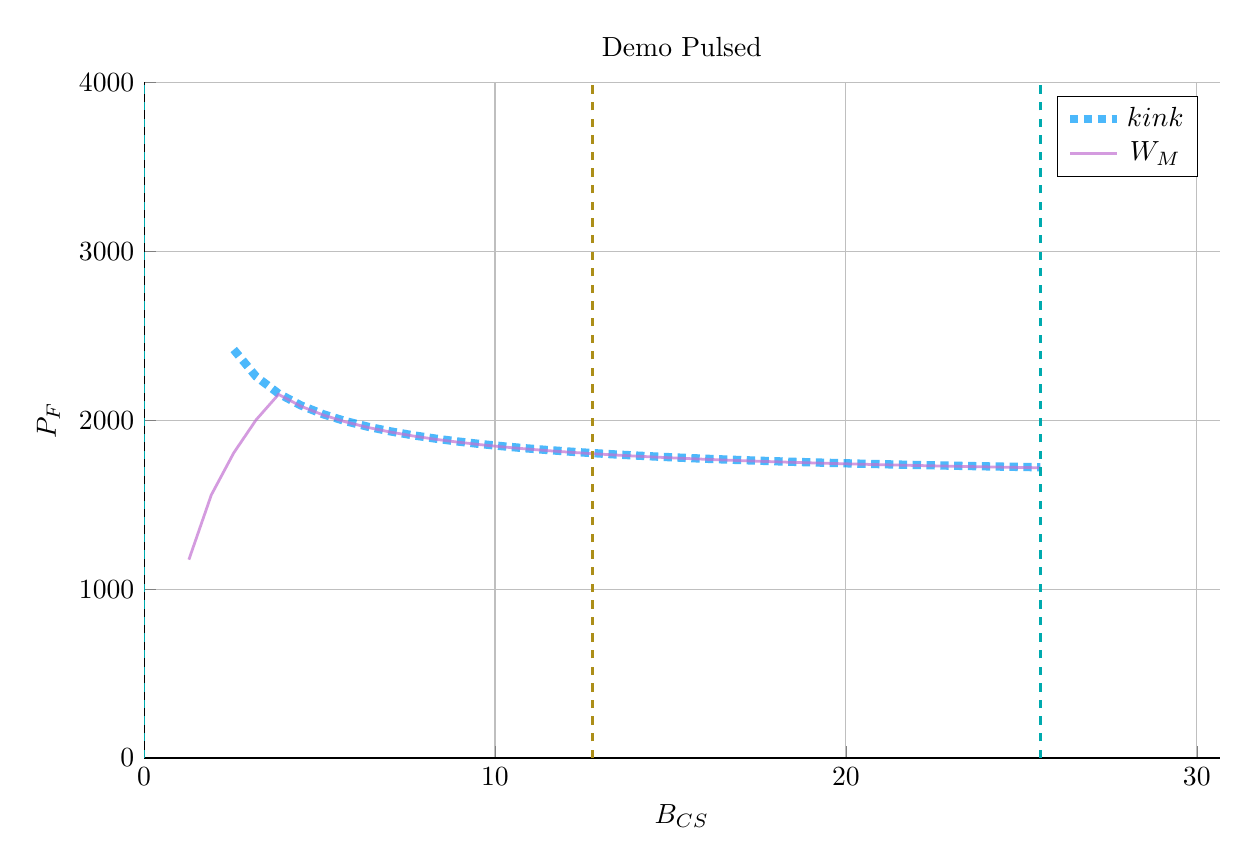
\begin{tikzpicture}[]
\begin{axis}[height = {101.6mm}, ylabel = {${P}_{F}$}, title = {Demo Pulsed}, xmin = {0.0}, xmax = {30.647999999999996}, ymax = {4000.0}, xlabel = {${B}_{CS}$}, {unbounded coords=jump, scaled x ticks = false, xticklabel style={rotate = 0}, xmajorgrids = true, xtick = {0.0,10.0,20.0,30.0}, xticklabels = {0,10,20,30}, xtick align = inside, axis lines* = left, scaled y ticks = false, yticklabel style={rotate = 0}, ymajorgrids = true, ytick = {0.0,1000.0,2000.0,3000.0,4000.0}, yticklabels = {0,1000,2000,3000,4000}, ytick align = inside, axis lines* = left,     xshift = 0.0mm,
    yshift = 0.0mm,
    axis background/.style={fill={rgb,1:red,1.00000000;green,1.00000000;blue,1.00000000}}
, colorbar style={title=}}, ymin = {0.0}, width = {152.4mm}]\addplot+ [color = {rgb,1:red,0.00000000;green,0.60560316;blue,0.97868012},
draw opacity=0.7,
line width=3,
dotted,mark = none,
mark size = 2.0,
mark options = {
    color = {rgb,1:red,0.00000000;green,0.00000000;blue,0.00000000}, draw opacity = 0.7,
    fill = {rgb,1:red,0.00000000;green,0.60560316;blue,0.97868012}, fill opacity = 0.7,
    line width = 1,
    rotate = 0,
    solid
}]coordinates {
(2.554, 2418.439490660037)
(3.1925, 2258.667693929749)
(3.831, 2158.0434330029475)
(4.4695, 2087.6944206835706)
(5.108, 2035.1850409704718)
(5.7465, 1994.1965229213151)
(6.385, 1961.1441091669103)
(7.0235, 1933.826748790783)
(7.662, 1910.809955252131)
(8.3005, 1891.1142191277927)
(8.939, 1874.045166007475)
(9.5775, 1859.0951637532023)
(10.216, 1845.8834195623997)
(10.8545, 1834.1179730892675)
(11.493, 1823.5707253838252)
(12.1315, 1814.0605347693095)
(12.77, 1805.4414957120475)
(13.4085, 1797.5944815414484)
(14.047, 1790.4213179193448)
(14.6855, 1783.840134166425)
(15.324, 1777.781969664348)
(15.9625, 1772.1884340879249)
(16.601, 1767.0095972933589)
(17.2395, 1762.2024944996933)
(17.878, 1757.7298713228834)
(18.5165, 1753.5594201574)
(19.155, 1749.6627140975622)
(19.7935, 1746.0147788945287)
(20.432, 1742.5935778099401)
(21.0705, 1739.3793742056532)
(21.709, 1736.35482098222)
(22.3475, 1733.5042719541648)
(22.986, 1730.8135737806701)
(23.6245, 1728.2702184672714)
(24.263, 1725.8626428941761)
(24.9015, 1723.5806118852602)
(25.54, 1721.4146017114554)
};
\addlegendentry{$kink$}
\addplot+ [color = {rgb,1:red,0.76444018;green,0.44411178;blue,0.82429754},
draw opacity=0.7,
line width=1,
solid,mark = none,
mark size = 2.0,
mark options = {
    color = {rgb,1:red,0.00000000;green,0.00000000;blue,0.00000000}, draw opacity = 0.7,
    fill = {rgb,1:red,0.76444018;green,0.44411178;blue,0.82429754}, fill opacity = 0.7,
    line width = 1,
    rotate = 0,
    solid
}]coordinates {
(1.277, 1174.4191595640114)
(1.9155, 1557.5099838793772)
(2.554, 1806.3330313588413)
(3.1925, 2002.266281526456)
(3.831, 2152.948912848028)
(4.4695, 2082.9342814002794)
(5.108, 2030.6738841896818)
(5.7465, 1989.8799521445594)
(6.385, 1956.9849582412296)
(7.0235, 1929.7982968068923)
(7.662, 1906.8921995146331)
(8.3005, 1887.2917453417733)
(8.939, 1870.3057585821527)
(9.5775, 1855.4289762406506)
(10.216, 1842.2823256076385)
(10.8545, 1830.575224059819)
(11.493, 1820.0806153930123)
(12.1315, 1810.6181808889562)
(12.77, 1802.0426638004947)
(13.4085, 1794.2355420887463)
(14.047, 1787.0990590472247)
(14.6855, 1780.5516755814833)
(15.324, 1774.524841644359)
(15.9625, 1768.9603836664687)
(16.601, 1763.8086152609226)
(17.2395, 1759.0267819242679)
(17.878, 1754.5778384698829)
(18.5165, 1750.4295358069392)
(19.155, 1746.5536228804472)
(19.7935, 1742.9252430663948)
(20.432, 1739.5224273045656)
(21.0705, 1736.3256505161612)
(21.709, 1733.3175403646217)
(22.3475, 1730.482506673844)
(22.986, 1727.8065934950305)
(23.6245, 1725.2772187330588)
(24.263, 1722.8829728498188)
(24.9015, 1720.6135803737259)
(25.54, 1718.4596602703402)
};
\addlegendentry{$W_M$}
\addplot+ [color = {rgb,1:red,0.67554396;green,0.55566233;blue,0.09423434},
draw opacity=1.0,
line width=1,
dashed,mark = none,
mark size = 2.0,
mark options = {
    color = {rgb,1:red,0.00000000;green,0.00000000;blue,0.00000000}, draw opacity = 1.0,
    fill = {rgb,1:red,0.67554396;green,0.55566233;blue,0.09423434}, fill opacity = 1.0,
    line width = 1,
    rotate = 0,
    solid
},forget plot]coordinates {
(12.77, 0.0)
(12.77, 4000.0)
};
\addplot+ [color = {rgb,1:red,0.00000048;green,0.66575898;blue,0.68099695},
draw opacity=1.0,
line width=1,
dashed,mark = none,
mark size = 2.0,
mark options = {
    color = {rgb,1:red,0.00000000;green,0.00000000;blue,0.00000000}, draw opacity = 1.0,
    fill = {rgb,1:red,0.00000048;green,0.66575898;blue,0.68099695}, fill opacity = 1.0,
    line width = 1,
    rotate = 0,
    solid
},forget plot]coordinates {
(0.0, 0.0)
(0.0, 4000.0)
};
\addplot+ [color = {rgb,1:red,0.00000048;green,0.66575898;blue,0.68099695},
draw opacity=1.0,
line width=1,
dashed,mark = none,
mark size = 2.0,
mark options = {
    color = {rgb,1:red,0.00000000;green,0.00000000;blue,0.00000000}, draw opacity = 1.0,
    fill = {rgb,1:red,0.00000048;green,0.66575898;blue,0.68099695}, fill opacity = 1.0,
    line width = 1,
    rotate = 0,
    solid
},forget plot]coordinates {
(25.54, 0.0)
(25.54, 4000.0)
};
\end{axis}

\end{tikzpicture}

		\end{adjustbox}
        \caption{Demo Pulsed Fusion Power}
    \end{subfigure}	
    \hfill \hfill ~\\ ~\\ ~\\
    \caption{Pulsed $B_{CS}$ Sensitivity}
    \label{fig:pulsed_sensitivities}
\end{figure*}

\begin{figure*}
    \centering
    \hfill 
    \begin{subfigure}[t]{0.45\textwidth}
        \centering
		\begin{adjustbox}{width=\textwidth}
			\Large
			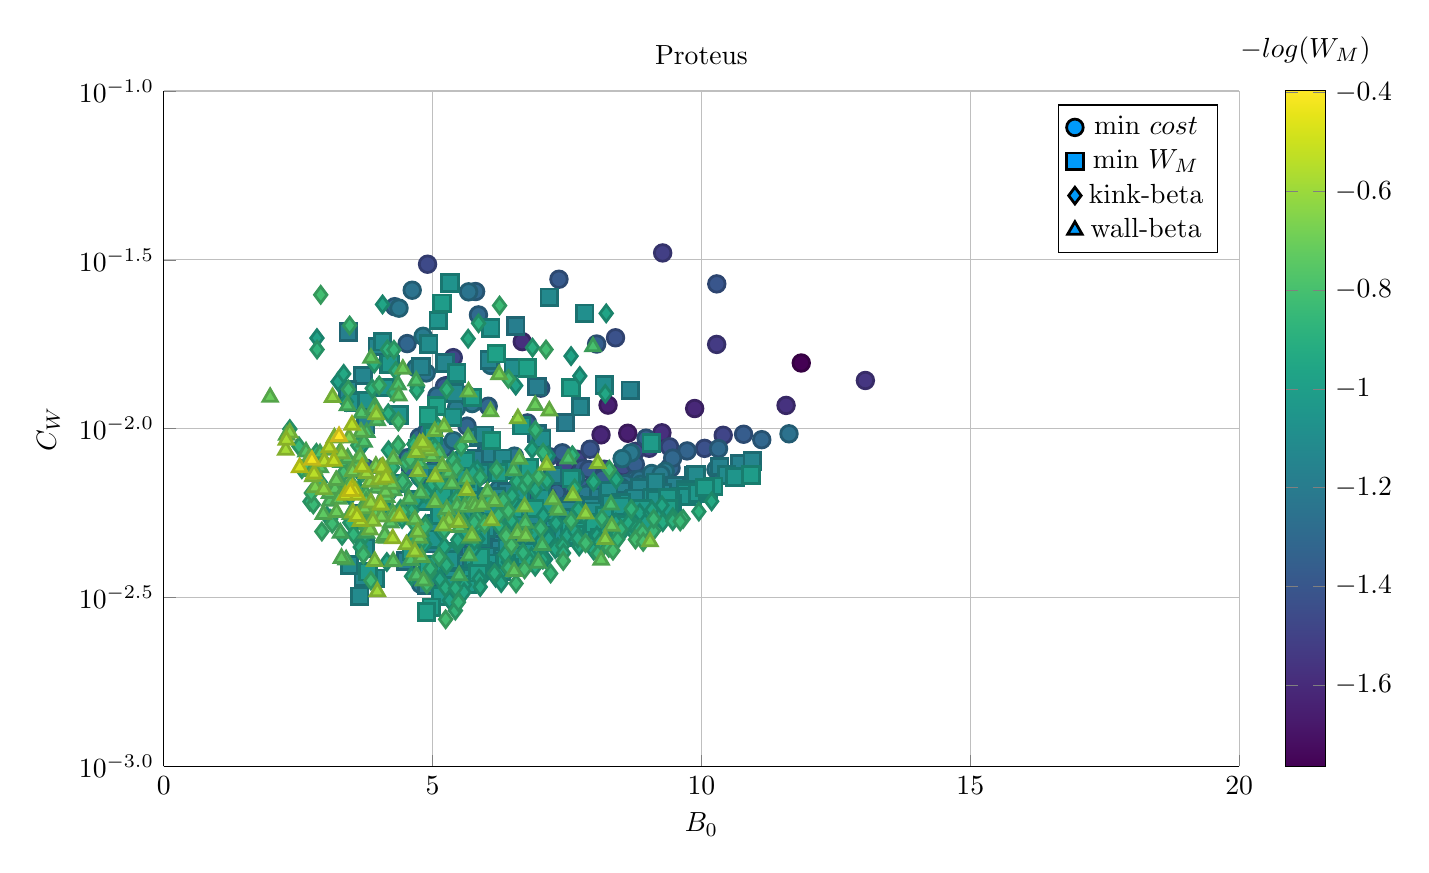
\begin{tikzpicture}[]
\begin{axis}[colorbar = {true}, height = {101.6mm}, ylabel = {${C}_{W}$}, title = {Proteus}, xmin = {0.0}, xmax = {20.0}, ymax = {0.1}, ymode = {log}, xlabel = {${B}_{0}$}, {unbounded coords=jump, scaled x ticks = false, xticklabel style={rotate = 0}, xmajorgrids = true, xtick = {0.0,5.0,10.0,15.0,20.0}, xticklabels = {0,5,10,15,20}, xtick align = inside, axis lines* = left, scaled y ticks = false, yticklabel style={rotate = 0}, log basis y=10, ymajorgrids = true, ytick = {0.001,0.0031622776601683794,0.01,0.03162277660168379,0.1}, yticklabels = {$10^{-3.0}$,$10^{-2.5}$,$10^{-2.0}$,$10^{-1.5}$,$10^{-1.0}$}, ytick align = inside, axis lines* = left,     xshift = 0.0mm,
    yshift = 0.0mm,
    axis background/.style={fill={rgb,1:red,1.00000000;green,1.00000000;blue,1.00000000}}
, colormap={plots}{rgb=(0.26700400,0.00487400,0.32941500), rgb=(0.27794100,0.05632400,0.38119100), rgb=(0.28291000,0.10539300,0.42690200), rgb=(0.28229000,0.14591200,0.46151000), rgb=(0.27619400,0.19007400,0.49300100), rgb=(0.26514500,0.23295600,0.51659900), rgb=(0.25042500,0.27429000,0.53310300), rgb=(0.23360300,0.31382800,0.54391400), rgb=(0.21813000,0.34743200,0.55003800), rgb=(0.20123900,0.38367000,0.55429400), rgb=(0.18555600,0.41857000,0.55675300), rgb=(0.17117600,0.45253000,0.55796500), rgb=(0.15772900,0.48593200,0.55801300), rgb=(0.14618000,0.51541300,0.55682300), rgb=(0.13374300,0.54853500,0.55354100), rgb=(0.12346300,0.58168700,0.54744500), rgb=(0.11948300,0.61481700,0.53769200), rgb=(0.12632600,0.64410700,0.52531100), rgb=(0.15014800,0.67663100,0.50658900), rgb=(0.19109000,0.70836600,0.48228400), rgb=(0.24607000,0.73891000,0.45202400), rgb=(0.31192500,0.76782200,0.41558600), rgb=(0.37777900,0.79178100,0.37793900), rgb=(0.45867400,0.81636300,0.32972700), rgb=(0.54552400,0.83803900,0.27562600), rgb=(0.63690200,0.85654200,0.21662000), rgb=(0.73088900,0.87191600,0.15602900), rgb=(0.81457600,0.88339300,0.11034700), rgb=(0.90631100,0.89485500,0.09812500), rgb=(0.99324800,0.90615700,0.14393600)}, colorbar style={title=$-log( W_M )$}}, ymin = {0.001}, width = {152.4mm}]\addplot+[scatter, scatter src=explicit, only marks = {true}, color = {rgb,1:red,0.00000000;green,0.60560316;blue,0.97868012},
draw opacity=1,
line width=0,
solid,mark = *,
mark size = 3.0,
mark options = {
    color = {rgb,1:red,0.00000000;green,0.00000000;blue,0.00000000}, draw opacity = 1.0,
    fill = {rgb,1:red,0.00000000;green,0.60560316;blue,0.97868012}, fill opacity = 1,
    line width = 1,
    rotate = 0,
    solid
}] coordinates {
(11.855851167264671, 0.015650867313707448) [-1.7651507846396934]
(8.62894306410229, 0.009694646552347688) [-1.652530796858066]
(8.262669569295957, 0.011744038729478485) [-1.647000146345283]
(8.132345586482765, 0.009590177278586947) [-1.6184546481250472]
(9.87352129314419, 0.011474300333025303) [-1.6124908438767973]
(9.26466071494926, 0.00972401084478665) [-1.5828949402967583]
(6.667811597046653, 0.018106858351787505) [-1.577618500437912]
(11.573395463568893, 0.011719738653164523) [-1.56873554690934]
(5.264528343635174, 0.013419897432724169) [-1.5599002750009094]
(13.048135395345042, 0.013892471464509717) [-1.5518482038436605]
(10.282796584070674, 0.017767343192357253) [-1.5302287668791192]
(9.278542294221232, 0.033146306422516245) [-1.5115301730224102]
(7.5044360623009565, 0.007510212646674021) [-1.5013825191439996]
(9.02784009554164, 0.008751202105526691) [-1.4958902811815062]
(8.710683108208965, 0.00816949735167802) [-1.4892617900728689]
(7.687377168804008, 0.008118078139228204) [-1.4884348201277007]
(10.404534949568816, 0.009559158760396884) [-1.4866425610729714]
(5.384524713145202, 0.01623184139531336) [-1.4835478223239928]
(7.472857057569771, 0.007837831837729894) [-1.4780728724015184]
(4.906484287411937, 0.03069401611625924) [-1.4650031348255397]
(7.111580297007043, 0.006765803188842749) [-1.4601242927308113]
(8.773685022223647, 0.008568870415676909) [-1.453691298071198]
(8.545510256202396, 0.007723927816166263) [-1.4489094778079963]
(7.070436548811644, 0.006162431971740805) [-1.432973868001932]
(6.884154096232421, 0.006329451983138475) [-1.4325147285303634]
(9.405921329983288, 0.008839617844718544) [-1.4268866569895065]
(10.057985274469397, 0.008744700190770928) [-1.4268347679685771]
(8.401821549997786, 0.018590297650719324) [-1.4237681445033143]
(8.189937032371649, 0.007587250291191641) [-1.4234658725845162]
(8.234578254729767, 0.007390656211515189) [-1.4109108269606008]
(7.92991212471289, 0.008694085637837138) [-1.4079262096010774]
(6.59839258184741, 0.00634066157530613) [-1.407330123320285]
(10.284931156770094, 0.026840973164111593) [-1.3996791570309395]
(7.3137838143058795, 0.007040053838733538) [-1.3974870797438]
(5.221820332167986, 0.013359280479800206) [-1.3946269662443698]
(7.785957307166937, 0.007634837530984513) [-1.3905305073664083]
(7.069469201177765, 0.006488653571629467) [-1.3895960301339119]
(6.200523563918331, 0.00554611680879456) [-1.381931002288656]
(7.340133149046422, 0.00695131625200887) [-1.3818272949203658]
(7.349866215424601, 0.027704627448181397) [-1.3812563757949996]
(7.351199097200025, 0.00681167564679013) [-1.379699079550137]
(8.120289345307025, 0.006715817539753603) [-1.376650573885692]
(7.90274300232169, 0.00757067906104037) [-1.3758581110553065]
(7.565484576443418, 0.006499559071472007) [-1.375220700855124]
(7.688718501611012, 0.00646934556613389) [-1.3742348635950123]
(7.005633077388933, 0.0063267927368600325) [-1.3713423550361032]
(7.166534585210968, 0.008267480512087599) [-1.370057699317172]
(5.695615872659735, 0.004988896324536347) [-1.3686239973313072]
(6.620180775083285, 0.005540386026064644) [-1.3680076928767484]
(5.712356159098289, 0.005024205798518008) [-1.3672266212882762]
(10.783439028923059, 0.009628839399324697) [-1.3667105305870977]
(6.000471468140266, 0.0050592629231849704) [-1.3651176317240314]
(8.050752136473724, 0.017814080806893125) [-1.3612722200713383]
(8.77043990632116, 0.007840171434328094) [-1.360737823431438]
(7.010340303297389, 0.013182987051350502) [-1.3596008789905631]
(7.295294539644262, 0.006730765435871485) [-1.3568098625263256]
(6.641599582701438, 0.005632641769207446) [-1.3562925407270994]
(6.645748730966029, 0.005613911931897123) [-1.3540300242042478]
(6.054699810485283, 0.005176189759381431) [-1.3527684291391184]
(9.401252816575663, 0.007678792615766904) [-1.3513432280511455]
(5.581708167132495, 0.006888425944911811) [-1.3508742741062625]
(7.803535098905909, 0.006674090356682625) [-1.348444904526092]
(6.76411548346407, 0.010402669872398145) [-1.3482429808137002]
(8.969455503638764, 0.009376571407375644) [-1.3481015746033576]
(5.634510628688515, 0.012583797530216616) [-1.34746159692277]
(8.156032796881272, 0.007115527316776566) [-1.3450418873098828]
(7.056939291922313, 0.006464286011476574) [-1.3449397649071608]
(7.240799475525162, 0.006186516144095541) [-1.344834769873685]
(6.571134452649435, 0.0053864817732829605) [-1.3436955024234147]
(7.4120702527384665, 0.00848434463520388) [-1.3426163725681677]
(5.934011898969639, 0.004938310227983135) [-1.3374912582230194]
(7.37766442956072, 0.006636608478826529) [-1.335539302100867]
(5.026669706190863, 0.007606581585076429) [-1.3352915983538123]
(6.825792187162438, 0.006029019944814239) [-1.331337874103357]
(9.732916904654346, 0.008594819258321628) [-1.3310780697195672]
(5.698038434377145, 0.004728216221281147) [-1.3292068036291638]
(6.854283769326888, 0.005953363383436291) [-1.32828646244698]
(4.7527705925878685, 0.009441137210103956) [-1.3280975618898123]
(6.452485475407575, 0.005079524630506098) [-1.3278697867431468]
(6.6282734062471, 0.005749625528658903) [-1.327757292865828]
(7.362442088263758, 0.006249734903697681) [-1.3253106415861637]
(6.357926345811093, 0.005155209960292018) [-1.3237407060184172]
(9.434691757978365, 0.007650804529712704) [-1.3217246458754282]
(5.945683748997239, 0.004926318213851794) [-1.319376268743699]
(5.716699212704698, 0.004774448071559269) [-1.3182101821558738]
(7.9999703999657505, 0.0066268624262571275) [-1.31770129332637]
(4.526018058829261, 0.017867829271260238) [-1.3171626271127284]
(7.307142270921693, 0.006479743346210051) [-1.3144438328362922]
(5.64022055353738, 0.010177994071422254) [-1.314397397461996]
(11.121291715489328, 0.009279261565995508) [-1.3134452963620502]
(6.890660641840135, 0.005896178522672516) [-1.3126768401499638]
(5.8496112618323926, 0.007223214696135702) [-1.3123916957087167]
(3.755618871416242, 0.007643344629724278) [-1.3117090270675453]
(6.965828665871357, 0.0062843154751196315) [-1.3112976001573549]
(7.132942553696917, 0.006316305209750007) [-1.3102933400586538]
(6.034623082086722, 0.011655743235665423) [-1.3084666426112759]
(9.464190150712176, 0.008181643780093392) [-1.3081739820914746]
(6.735484315816856, 0.005920113041607297) [-1.3081169022767745]
(6.329532230716051, 0.005266304291939928) [-1.3075986397555424]
(6.949512174456946, 0.0056632699287416785) [-1.3038897119548887]
(5.7123865302563095, 0.004515583648974614) [-1.3034916079905217]
(4.588431546307119, 0.00762405310841983) [-1.301506470226052]
(5.8529754306366, 0.021723513711501174) [-1.2978787946122285]
(6.763583440942078, 0.005860560202229156) [-1.297460949292816]
(5.79974352272628, 0.02547444831481485) [-1.2953226778576867]
(4.294506467374343, 0.022974551007964673) [-1.2951062787178942]
(10.317711969577175, 0.008727794605170999) [-1.2946978796261759]
(7.030442720189729, 0.00606442154900928) [-1.293243062455323]
(6.3155245633398005, 0.00478216163852665) [-1.2916316854649297]
(5.594153930448576, 0.004505685536187866) [-1.291573412415986]
(7.0608047385200905, 0.006201757851874389) [-1.2910367642815292]
(8.746159160738731, 0.007056272547770033) [-1.2894268757747884]
(5.790961836119614, 0.004812007322004063) [-1.2891780169645117]
(7.13931972393237, 0.005900795309436559) [-1.2883016772579983]
(5.642350264315365, 0.004575860387174974) [-1.2877120777365891]
(5.500511487756749, 0.007501625869556503) [-1.2825608117529994]
(5.1870060839860015, 0.004048206616482656) [-1.2803416949249293]
(5.0793762257146975, 0.012501014524680899) [-1.2790944723531177]
(4.900710067477188, 0.009849033693022476) [-1.2789599032268324]
(5.416336002756713, 0.004266328381972482) [-1.278637308935949]
(7.047880217226236, 0.00602317781329061) [-1.2752962713941192]
(4.537987048593646, 0.008202673797589401) [-1.2724318730764337]
(6.7947527911354095, 0.005313590913225172) [-1.26778944603233]
(7.547856502776895, 0.005746237915345085) [-1.2652894696394015]
(8.337373800803634, 0.0063394092295352205) [-1.263844406219344]
(5.839234828237175, 0.004670640784960837) [-1.2622412045786418]
(6.307588148065544, 0.005025369604276285) [-1.2622057750392766]
(6.369182324037021, 0.004715175023029078) [-1.2568407944078956]
(7.25221896281004, 0.005515822538041083) [-1.2564369672634057]
(5.207422458409709, 0.008763742702873716) [-1.255580803936347]
(8.846964102011665, 0.007090160917314494) [-1.2542825781236586]
(11.62801313878366, 0.009658252430988482) [-1.253606675738751]
(6.586437041421525, 0.005078101074449218) [-1.2533258835374417]
(5.896819232149536, 0.004668333949768413) [-1.252740293490489]
(7.218625057420257, 0.005623439530060779) [-1.2512906609771755]
(4.770007649977626, 0.007192663750971734) [-1.2505906665339703]
(6.391248250395476, 0.004753912504004936) [-1.2505667349102745]
(6.722228809625436, 0.00547669175115548) [-1.2505409706978425]
(5.9975644347104575, 0.008585550973626429) [-1.2504311283223648]
(6.220483255591395, 0.00536142422310656) [-1.2495193060816674]
(7.131398255569569, 0.005891517799670805) [-1.2472203996667584]
(4.620896334693883, 0.025703839631456088) [-1.246340221801285]
(5.634708074324937, 0.004426672964739238) [-1.246337044553182]
(6.0053836269885, 0.004733745531528537) [-1.2444533586241864]
(6.122472771064873, 0.004373459187272198) [-1.2410504069560844]
(4.881468969197191, 0.014622918962551527) [-1.2404616678069278]
(5.669873863181108, 0.025422666134658947) [-1.2402101811954278]
(9.159921449108527, 0.00699405114862055) [-1.2399625556579728]
(6.619988989498716, 0.005459593535350185) [-1.2395775558220574]
(4.0721743569002395, 0.006780135026174841) [-1.238968027160994]
(8.487125648729805, 0.006381273355008305) [-1.2381935518916032]
(5.785136288326493, 0.005454977773134567) [-1.2372164242860222]
(7.805870043590986, 0.006162937475975255) [-1.2359322527835273]
(6.521775930847536, 0.008295248979234676) [-1.2345953253761524]
(7.299795216034374, 0.005661235915534237) [-1.2333782101635051]
(6.654376116038794, 0.005116145429327062) [-1.2329256482335589]
(8.586321868785943, 0.0068738253515159406) [-1.2318041138227]
(5.871716076416853, 0.007759607253139788) [-1.2286780396839752]
(5.525881431830733, 0.004270512991179436) [-1.225800447150557]
(4.37566370657649, 0.022744869820021597) [-1.2237626122718148]
(5.386416012885563, 0.009221148903357415) [-1.2192315569877235]
(5.735606858683557, 0.011868028475244749) [-1.2191811590789894]
(8.68706974133124, 0.008481483201532794) [-1.2185680785343938]
(8.63032181590475, 0.00622802822970762) [-1.2179132583990178]
(8.508158073563377, 0.006703260233628488) [-1.2171472173843672]
(7.953691408978824, 0.00633213628058925) [-1.2167448502658762]
(6.081331959057098, 0.015392818825938645) [-1.2162995250149307]
(5.225401290559421, 0.003872910530196867) [-1.215703789534109]
(5.988978974443945, 0.004720977485089404) [-1.2156312790675603]
(9.073087462786646, 0.00736963569440644) [-1.2145283350978044]
(7.217725198328268, 0.005383150867826381) [-1.214317974252912]
(5.536577745729214, 0.004178935326843822) [-1.2138536176262873]
(4.776559777248383, 0.0034641548226198885) [-1.2119360055173332]
(5.211688187540344, 0.0038140534914709043) [-1.2104347246988538]
(10.269380266980404, 0.007570292211977012) [-1.2084631186053005]
(6.918845939903695, 0.0052385995930077645) [-1.2083264519217767]
(7.0692693982238906, 0.005083028024589718) [-1.2073346872626274]
(5.874112036399968, 0.004039129704078142) [-1.2071975929322125]
(4.690082401892927, 0.01513911751066285) [-1.2067840670536927]
(7.861161945792819, 0.006395373245847939) [-1.206736577191552]
(9.326423266814658, 0.007483645463069493) [-1.2065799786199445]
(8.029413669351802, 0.005698374888186277) [-1.203843641047789]
(6.959732144718079, 0.005550896360654382) [-1.203724365314369]
(6.960477287319412, 0.005010777712400389) [-1.2024406864855146]
(7.654476699386534, 0.007157947201399507) [-1.2021169810907544]
(4.823547237227045, 0.01877759730610099) [-1.2015933815507112]
(6.062862639710857, 0.004489267037355289) [-1.2014423796656961]
(8.999102001729389, 0.006374667856956503) [-1.2011965112492808]
(7.2717504340335415, 0.00572395742880883) [-1.2005427289121806]
(6.227413325881237, 0.0066192080125215165) [-1.1994215784439877]
(9.247503176233229, 0.007316062816603203) [-1.1975084180232178]
(5.443249511926066, 0.011502671870448664) [-1.1972619972446426]
(6.742357647461489, 0.005266662336518346) [-1.1967371969067386]
(5.926964832086266, 0.004368135902166705) [-1.1965134818457024]
(8.524769827029726, 0.008154332104698897) [-1.196084536648355]
(8.867575034400405, 0.006843978332329513) [-1.1943424204563022]
(6.457339766119646, 0.005029914775543452) [-1.1908054127888088]
};
\addlegendentry{min $cost$}
\addlegendentry{min $W_M$}
\addlegendentry{kink-beta}
\addlegendentry{wall-beta}
\addplot+[scatter, scatter src=explicit, only marks = {true}, color = {rgb,1:red,0.00000000;green,0.60560316;blue,0.97868012},
draw opacity=1,
line width=0,
solid,mark = square*,
mark size = 3.0,
mark options = {
    color = {rgb,1:red,0.00000000;green,0.00000000;blue,0.00000000}, draw opacity = 1.0,
    fill = {rgb,1:red,0.00000000;green,0.60560316;blue,0.97868012}, fill opacity = 1,
    line width = 1,
    rotate = 0,
    solid
}] coordinates {
(7.4724590738720655, 0.010422279639263054) [-1.1890033537880158]
(6.938996985119089, 0.009658294464102987) [-1.1883675827161198]
(6.9393893920794385, 0.013313745665171912) [-1.1879538738656286]
(6.377850385556073, 0.006487414571263668) [-1.1878029685724296]
(6.547487324963764, 0.020145877705477357) [-1.186260879134981]
(8.029613686159495, 0.005801884747670386) [-1.1859242026174677]
(5.6874025972941205, 0.004217349677698315) [-1.183889066210908]
(7.827309596895398, 0.0058827996938258294) [-1.1830291222504283]
(5.8219713598117036, 0.008160599297710009) [-1.1826268505607591]
(6.946718058585209, 0.004857174007518612) [-1.182365307189366]
(3.434094114791118, 0.01935279381255584) [-1.1822251925764147]
(6.23809783755075, 0.00447855648592392) [-1.1813612663460882]
(5.88781791976068, 0.00428725320402622) [-1.1785285195809967]
(4.505121226933233, 0.004053651772674214) [-1.1775655951090325]
(6.553162158329651, 0.005121496915389368) [-1.17705398157876]
(5.8303432949169745, 0.005890819973806921) [-1.1767452937515073]
(8.807822926389145, 0.006104718148251412) [-1.1766083315756861]
(4.18691738643155, 0.01556268699280997) [-1.173888237216638]
(7.55203601905607, 0.005882961839613334) [-1.1734465174435744]
(5.819836385827624, 0.005961179911412564) [-1.1729466514857931]
(9.116693027577789, 0.006287276174883399) [-1.172839252676928]
(3.659189590525744, 0.005599267038542826) [-1.1727769211527406]
(7.004035835152084, 0.005070632392189801) [-1.1727372361954858]
(4.897086463141796, 0.003434292526080427) [-1.1726542785062386]
(8.087708955601924, 0.0062657093568900535) [-1.1703764252048678]
(6.7024429891400565, 0.004942047034638912) [-1.1699166462753263]
(5.893015258208656, 0.004183590560340062) [-1.1681831393061217]
(7.479710666339309, 0.005170881199231806) [-1.1671080842733117]
(9.508375514310952, 0.006777996547666784) [-1.1655606692177785]
(6.075560203652315, 0.008402469668507205) [-1.165303541813206]
(6.61932998550545, 0.004666935296152095) [-1.1643973078802388]
(6.286558265163782, 0.004663766235492665) [-1.1632535008384055]
(5.050068824721165, 0.004566940606242733) [-1.1631989573193973]
(7.688714523679582, 0.0054331000812183365) [-1.1630392685982025]
(8.505800422917172, 0.006544368204474158) [-1.1625753891662707]
(8.975209897762664, 0.006511116933487475) [-1.1617936783337066]
(8.380983437312786, 0.006126048639979384) [-1.159367616011031]
(8.67470730810651, 0.012995381528200805) [-1.1593260324319568]
(5.960621269295445, 0.004013416769217783) [-1.1592024857112633]
(6.282535161243701, 0.004530529794416821) [-1.1590403977294572]
(10.712436821713085, 0.007867971330715704) [-1.1589428109110296]
(7.099415207654768, 0.005330271588661515) [-1.158451320077056]
(10.3395352744249, 0.007724720119696045) [-1.157468772898154]
(6.536306152444655, 0.004436262085616985) [-1.1570637161067505]
(9.855000808062698, 0.007249642226094706) [-1.1563966451418943]
(5.856384724795581, 0.009420901412013665) [-1.1561531921827275]
(7.454679880823048, 0.0057898611640113395) [-1.1538328200442942]
(5.14753239685863, 0.007237376261288284) [-1.1525173430901554]
(6.856563325018079, 0.004881019954742076) [-1.1522162283529644]
(7.618840457764884, 0.0059379940430840635) [-1.151968932860403]
(8.398440991699191, 0.0061407721476487214) [-1.1511586507355254]
(4.781165601129724, 0.015255960449664327) [-1.1509834966159156]
(6.247011281135245, 0.004419080970160178) [-1.1503660387736743]
(3.7553680100049234, 0.01032617135589161) [-1.1500086948877408]
(5.5152996897670015, 0.004014883666259908) [-1.1494080253790357]
(7.800728278542519, 0.005291422749753008) [-1.1493093072503229]
(6.054088477025007, 0.01598351560152435) [-1.1489823622220707]
(5.411295562966824, 0.003915099463846501) [-1.1484511044037433]
(7.052045109627868, 0.005020529922825154) [-1.1483999797493492]
(5.28488049549897, 0.0034947010100993764) [-1.147064765638366]
(7.62011089503286, 0.005859550653426385) [-1.1465028274549764]
(7.468210164743146, 0.005641165149475234) [-1.144883586902141]
(5.595946792423691, 0.007176119328254024) [-1.144368544047569]
(10.943656185786155, 0.00802165691682325) [-1.1435280806157744]
(7.908061023064291, 0.005447269817044685) [-1.1433393449411435]
(8.854582349908517, 0.006668732693209443) [-1.143332108158641]
(6.549837080949351, 0.004886014774808058) [-1.143184585873657]
(3.9729755898485215, 0.017515494611674454) [-1.1428249654095861]
(3.703954177548893, 0.014377117697389604) [-1.1427984862828113]
(3.4213090828497417, 0.013005276311642224) [-1.142397010267489]
(6.02709699747974, 0.005929095379259443) [-1.1423708774410877]
(5.231750077921478, 0.01565086593371781) [-1.1422424769576425]
(7.2349136535832095, 0.007266091038483963) [-1.140012696356206]
(7.647205004097057, 0.005840600330748377) [-1.1399465227440013]
(6.532016233135844, 0.00480284773560221) [-1.1387943392990294]
(7.523885505796154, 0.005752426766742318) [-1.1382802201938975]
(7.750130276532692, 0.011612930840038163) [-1.1380314198362265]
(9.276469763067444, 0.006446360072583165) [-1.137892443914052]
(5.952941013085345, 0.009562541252399106) [-1.1311113631375915]
(7.951426521304668, 0.005743536904522906) [-1.1302954325651586]
(5.952653119927932, 0.0041760314888273755) [-1.1295543261638465]
(8.253192497448524, 0.006161648966500728) [-1.129462828049983]
(5.512192429439468, 0.00369116854025651) [-1.1277963061708562]
(6.180741676638315, 0.006278926396423389) [-1.126807171194116]
(6.608627477861355, 0.004487529275565533) [-1.1267021554022474]
(9.14457555501132, 0.006938744439971839) [-1.1265761162904897]
(5.310301950330671, 0.004304336836767321) [-1.1261385034152473]
(7.969320198807478, 0.005917258047258142) [-1.1260458936236624]
(7.954215183655014, 0.005885263457738176) [-1.1250537668582923]
(6.771595293849517, 0.005616858230043609) [-1.124511019242948]
(6.641944516873176, 0.004843731890681865) [-1.1236988869720232]
(6.896134858333351, 0.005173923137495115) [-1.1235064786985465]
(3.7132325707792995, 0.003624821435760545) [-1.1232730371267585]
(4.936839162331792, 0.007429853985811719) [-1.1231293548483412]
(6.555316024199809, 0.005231942783984398) [-1.1209978185544383]
(6.304604592673814, 0.008169617815892689) [-1.1196911148335087]
(8.737416781995437, 0.0061580609115664325) [-1.1194748634113345]
(6.123815672401932, 0.004188882178419093) [-1.119418152841014]
(8.324353852438948, 0.005791769416647159) [-1.1191123923650526]
(6.830685941792606, 0.004931972266091366) [-1.1181736482095217]
(8.279157421008941, 0.005611347227289511) [-1.1176702646643628]
(7.172394160745635, 0.024480989089009208) [-1.1175403888423328]
(6.753756430979739, 0.004518885765871233) [-1.1174827013795072]
(8.76524294869496, 0.0062233325455323925) [-1.1174414411464733]
(5.952289891041446, 0.006299808378708293) [-1.1171134960728113]
(6.523754565443294, 0.004568184715721437) [-1.1171111976535804]
(5.4096290381473375, 0.012757776435747556) [-1.1168806186241906]
(9.896916686410892, 0.007305420869085463) [-1.1160945644374545]
(8.286804128590813, 0.005340773800773009) [-1.1139896885893594]
(5.399012890266871, 0.0036233885329560954) [-1.1123768792739945]
(8.296167355721272, 0.005311493039288053) [-1.1112153482766423]
(6.778775360762903, 0.0045000578497955725) [-1.1111283014916062]
(3.642453456441478, 0.003188662256079057) [-1.1108869662710774]
(6.918579935305505, 0.004842654136629077) [-1.1089922492653659]
(6.5071710234613676, 0.00452032863173795) [-1.108391782497311]
(7.258592477367294, 0.00535669926333167) [-1.1082929384878708]
(6.6776055936353265, 0.004745534590751309) [-1.1074346113685616]
(5.3226296796509205, 0.004323464728471098) [-1.1074227437950106]
(10.46985584146923, 0.007293078759243216) [-1.1069130893453907]
(3.4547855533452156, 0.003945456212149148) [-1.106325178133445]
(7.57975455174028, 0.004982808461571556) [-1.1060035644106432]
(5.06842585608741, 0.0052409052861536465) [-1.1038776732161713]
(5.698043204630489, 0.0065314531396132094) [-1.10351060592976]
(7.734654274692709, 0.005173060010686301) [-1.1022315889718237]
(6.228402773452205, 0.005951424789746293) [-1.1016702257969113]
(5.288893434740895, 0.007437806150470808) [-1.100448826904311]
(7.254453932047169, 0.005288339533793414) [-1.0998565094908217]
(6.807046489565401, 0.004337170224988449) [-1.0995498480529582]
(8.496667761878552, 0.005750254423520601) [-1.0992970719713648]
(6.506723144546308, 0.004423364554484401) [-1.0987351440216522]
(8.273277101596172, 0.006535275113176343) [-1.0983869460625248]
(7.024499917691516, 0.006822630998366228) [-1.0977261444257258]
(4.929559505548113, 0.017828562633364364) [-1.0969882385788774]
(6.546519891753608, 0.004407786879742766) [-1.096807077081938]
(6.299458688060015, 0.0041501216036249275) [-1.0962033310727437]
(5.917588131126826, 0.003972749736578854) [-1.0948458082881816]
(6.5027787367036485, 0.015155543307471772) [-1.093965318294314]
(8.191093731826841, 0.013471957430229371) [-1.093275686079877]
(5.765417917352738, 0.003923510470624812) [-1.0931318196649105]
(4.067683728143941, 0.01811006730780237) [-1.0926393639694263]
(5.643295069658257, 0.005671433069083637) [-1.09199330517098]
(5.33448260992027, 0.0035546432563184145) [-1.0916603258728452]
(5.996010919360583, 0.005082501155756355) [-1.091508438458307]
(6.130249778803564, 0.003922207642532424) [-1.0911853630489914]
(5.152309500808404, 0.007129588907950501) [-1.0896526200520398]
(6.613976143688219, 0.004468466025444819) [-1.088663441639713]
(7.828710312153846, 0.021949864805969728) [-1.0877780715734315]
(7.029871400370792, 0.009322832924906896) [-1.0870739196827126]
(6.6598420793586, 0.004672088916974179) [-1.0855818982110972]
(6.33097870945106, 0.004039319528471343) [-1.0844715994400023]
(7.702268833143657, 0.0053439960085053) [-1.0842780595786392]
(6.084754710909704, 0.005760793758021615) [-1.084266572782003]
(7.98999393987453, 0.00569380985136289) [-1.0839928767281124]
(5.068992476376386, 0.0039349920083461085) [-1.0828594792618813]
(9.086048642306793, 0.0062405207423892875) [-1.082853352734588]
(7.44906676523106, 0.0054577800846403015) [-1.0824719035597]
(5.375575122544495, 0.0035809652689903063) [-1.0824709528228211]
(7.386984140765724, 0.005148297391297789) [-1.0814366033908964]
(9.702271536107535, 0.006582162000449632) [-1.0809878234039578]
(9.614854186704672, 0.006301853688415234) [-1.0808972954130593]
(4.645688111866446, 0.006161790226168522) [-1.0797863646031054]
(3.927334262139488, 0.0036086053477567665) [-1.079163153355685]
(6.963971610592974, 0.004793357206410555) [-1.0780309855478056]
(8.244956752748422, 0.0054298508521766365) [-1.076806285491668]
(5.769697532800943, 0.00604411217248383) [-1.0765985094568509]
(7.283344319549832, 0.004828662165485411) [-1.0760641298404754]
(5.392578394594405, 0.005661819547798889) [-1.0757730303287785]
(3.7434225317786316, 0.00443044659495794) [-1.0744056068515366]
(7.7252366425534715, 0.005467468655559742) [-1.073726482715373]
(8.506016241294386, 0.006046667097602973) [-1.072815333291583]
(5.722077224788854, 0.006315687038558954) [-1.0718638391063322]
(3.5290681872248832, 0.011989877345034696) [-1.0710072465261937]
(5.408389828424612, 0.006287200186056995) [-1.0706716976099708]
(5.880603880610476, 0.00739594343637032) [-1.069478881808043]
(3.770984054785403, 0.012080600310741674) [-1.0679830462657767]
(9.144669371614333, 0.006138341400017388) [-1.0670572282884458]
(5.3325423351198395, 0.004085658341340117) [-1.0667391835901658]
(8.316799187366927, 0.006004004929014098) [-1.066302608545655]
(6.389619437625667, 0.004440975162005993) [-1.064104157833971]
(5.324355765249537, 0.026972932068461592) [-1.0640878812065675]
(6.511622532652898, 0.004395996587917252) [-1.0635820925869255]
(6.911249511094287, 0.004423420241739423) [-1.062988318250961]
(7.502962627592097, 0.00480727122317776) [-1.0628036997189863]
(5.469724443246719, 0.0034131330547271113) [-1.062700357913494]
(5.706475165604361, 0.0036974585830479817) [-1.0626514373993834]
(7.276669037534987, 0.004776499853086686) [-1.0610739421064752]
(6.526975357350624, 0.004144297606935685) [-1.0588352037418618]
(5.105089902831069, 0.0209014980088616) [-1.0585986545827941]
(4.374531653432859, 0.010988948677442597) [-1.057135771526312]
(4.122473679442906, 0.013241941603829825) [-1.056315661795303]
(6.078673477412938, 0.019862106250452566) [-1.0562734967702754]
(7.427558910001991, 0.004858658731965693) [-1.0561257856094448]
(7.01015270925273, 0.006223828461257365) [-1.0559814704124602]
(5.014809023336614, 0.004706089102701761) [-1.0555859489072712]
(6.029077134394886, 0.003994614402213268) [-1.0549803415205259]
(9.718000396033032, 0.006463993798881436) [-1.0545713902023608]
(5.896086527792721, 0.0038990516235787613) [-1.054205756099488]
(10.62632239203378, 0.007195479612398366) [-1.0536290024409787]
(9.830251746280974, 0.006286763322784177) [-1.0533216125601341]
(5.653429182632709, 0.004822724612666477) [-1.0529307720930816]
(7.148582094551358, 0.005656264568736301) [-1.0525850668019536]
(9.721783343528084, 0.006295530789348686) [-1.052552508886994]
(6.4747129291886205, 0.007550888758433211) [-1.0509835312174363]
(7.5553171987129115, 0.004904482654727138) [-1.0508250621973283]
(5.689433662550519, 0.006571304536184572) [-1.050680345054969]
(6.819358408267933, 0.004560195418506711) [-1.0506245233592775]
(5.372500908480495, 0.01080264515897382) [-1.0505217359121972]
(9.464104357867244, 0.00597835329976134) [-1.049317623712287]
(9.421645636318559, 0.00605275476812188) [-1.0490747591885061]
(6.83923495211403, 0.004511808104116367) [-1.0489907539423449]
(7.595014509377157, 0.0049153150140211965) [-1.0478434867034416]
(6.9492853284169565, 0.004616652674773231) [-1.0473758850488442]
(6.631954997333512, 0.006447737760929581) [-1.046767629611379]
(4.836574702453568, 0.006114416229637186) [-1.0460742739305466]
(5.447392742867525, 0.01461141466329314) [-1.0428746875530057]
(5.278008805745069, 0.0034297894059699906) [-1.0409932776852704]
(6.869290933859089, 0.004324846597058025) [-1.040720375777512]
(4.388359570069462, 0.0068957525832947) [-1.0400494553390642]
(7.730136216039545, 0.0047742837106654985) [-1.03963800286999]
(5.097390647393597, 0.0070972253563865) [-1.0394862991533038]
(5.705197239891871, 0.006107051538135721) [-1.0391370640013136]
(4.211114439903267, 0.015503036624972183) [-1.038354289214968]
(9.925180494788561, 0.006445735380428859) [-1.0380750082543837]
(8.392824243874195, 0.005205902574339689) [-1.0370263081612092]
(7.973811270774484, 0.005283195240312258) [-1.0365321066837632]
(8.49921904371083, 0.005892181423629392) [-1.0364145571368009]
(6.655649338522086, 0.010214094301379546) [-1.0358730287795153]
(6.272206414918943, 0.003781581128188247) [-1.0352797650690977]
(9.40142074331525, 0.0061316127141858145) [-1.0352425491421158]
(4.6061758509773245, 0.004345014451914255) [-1.0335536367675167]
(5.764426452876033, 0.00415632052734694) [-1.0319535365225938]
(9.372888478292797, 0.006253917955260214) [-1.031638330454266]
(5.729013310777877, 0.003613822408322808) [-1.0316283345953763]
(5.883030813164119, 0.00478160347928963) [-1.0312630056422283]
(6.556479558238363, 0.004326998549376461) [-1.030801418278412]
(6.395724956994062, 0.006039359373565179) [-1.0301227610636083]
(5.139256557257989, 0.005550817437725965) [-1.029015666765989]
(10.123332193763748, 0.006583295742064639) [-1.0288573869793878]
(6.568561456688728, 0.004204292638824563) [-1.0245024368116802]
(5.6039086370880105, 0.007145400138218064) [-1.0231385619546913]
(7.648719554707365, 0.004789677204757558) [-1.021449027000752]
(10.226601060349507, 0.00675373673736514) [-1.0213127693885564]
(5.153470412653239, 0.003193542226257652) [-1.0209276741398987]
(7.579001576207003, 0.007121099635585821) [-1.0202684704954939]
(3.8015765702844804, 0.0037708668397859442) [-1.0187837906200732]
(8.894908266877893, 0.005805595496214904) [-1.0179738483919518]
(9.066566182501706, 0.009070154520460257) [-1.0169425110693646]
(8.213444606213486, 0.00501503870041615) [-1.0162045101447212]
(10.062564168396998, 0.00670010251636303) [-1.0149810946438107]
(4.727731778507776, 0.008752580219573484) [-1.014353466976016]
(5.174769297851055, 0.023528952793841592) [-1.0140528730661398]
(8.195915051921629, 0.005527004085356763) [-1.0133093427968076]
(7.054369905297556, 0.004778958682375364) [-1.0128360857902137]
(5.031848935370691, 0.003842216867194081) [-1.0126834015105255]
(10.922140692684003, 0.007300503854095673) [-1.0124869131348806]
(5.915584448350069, 0.0038089628255598917) [-1.0084966915198963]
(5.602678326023923, 0.008048423371546378) [-1.005776006726422]
(7.544600594243294, 0.005136336479510988) [-1.0027757315503723]
(4.977942341177753, 0.0029594317443149176) [-1.002422823826331]
(5.642218938318191, 0.003459304695059543) [-1.0023352556688647]
(8.295019648678474, 0.004988217345842403) [-0.9994656987080655]
(7.070940189155582, 0.004649343635980374) [-0.9991953302395459]
(6.226711465325763, 0.007411548557741582) [-0.9991876183275935]
(6.419292049664728, 0.0038831217844692545) [-0.9971256954762724]
(4.887255844769486, 0.0028654321699102935) [-0.9968293366364798]
(7.7523402111694955, 0.004992975570566671) [-0.9965130838642419]
(5.890289877584987, 0.003830578946172306) [-0.9960911988132904]
(7.574296219984337, 0.013215773066776348) [-0.9953080727443692]
(9.012153601445592, 0.005338097758519931) [-0.994764309342816]
(9.386356586964215, 0.005798704578553127) [-0.9941918143808477]
(6.789856926677994, 0.007661762309327555) [-0.9939974184414383]
(5.741492166499531, 0.012372283627325148) [-0.9936895922796631]
(8.093840230774958, 0.0047417231470052315) [-0.9920762514365737]
(8.423301149042322, 0.005175409039233765) [-0.9891335090238219]
(6.5096125388500665, 0.005799134035216279) [-0.988320863141931]
(6.362065295698958, 0.003975692742134705) [-0.9873980470532571]
(6.898795759334327, 0.005803966541873779) [-0.9872638091155089]
(5.86662772167221, 0.005281651647264406) [-0.9871243344745786]
(5.00980677003057, 0.00954881671016918) [-0.9862026242600886]
(6.0980328290063905, 0.009231911938640338) [-0.9851939256634008]
(8.004532839270633, 0.005233428706224578) [-0.9845137991026185]
(6.760939557779194, 0.015110407509335635) [-0.9844063088607684]
(5.192252043701997, 0.006274740712107015) [-0.9843851675543582]
(6.182612803400956, 0.01666579340898781) [-0.9832677624207663]
(8.112468976523042, 0.004743145828135927) [-0.9823156156623659]
(5.841361480008224, 0.003744148435661381) [-0.9817957805945331]
(7.647006952351862, 0.0048552692105239565) [-0.9817262777133879]
(5.077285700891451, 0.01167873981501713) [-0.980944500204026]
(5.883453787587344, 0.004161496814710868) [-0.9808435285359967]
(4.920420200443467, 0.010903168023481107) [-0.9803069086017846]
(8.471906861597214, 0.005187973951951495) [-0.979926239566149]
(4.915731269106913, 0.0039527765780552285) [-0.9799255860420428]
};
\addlegendentry{min $cost$}
\addlegendentry{min $W_M$}
\addlegendentry{kink-beta}
\addlegendentry{wall-beta}
\addplot+[scatter, scatter src=explicit, only marks = {true}, color = {rgb,1:red,0.00000000;green,0.60560316;blue,0.97868012},
draw opacity=1,
line width=0,
solid,mark = diamond*,
mark size = 3.0,
mark options = {
    color = {rgb,1:red,0.00000000;green,0.00000000;blue,0.00000000}, draw opacity = 1.0,
    fill = {rgb,1:red,0.00000000;green,0.60560316;blue,0.97868012}, fill opacity = 1,
    line width = 1,
    rotate = 0,
    solid
}] coordinates {
(5.163569333804058, 0.0049343734079309275) [-0.9797193514246809]
(7.7377435890937285, 0.014326928101993836) [-0.9793649258547107]
(5.770648171127724, 0.004418560150536774) [-0.9793554194238832]
(4.7261265073999565, 0.007133046942930264) [-0.9793399260652301]
(4.749925847834237, 0.004527202123528333) [-0.9786718824413932]
(3.240965863210715, 0.013777079521683793) [-0.9784247640598123]
(8.408728218761828, 0.005278344797288595) [-0.9784156054323705]
(5.20936895107677, 0.004002965553163199) [-0.9772101816150688]
(6.546367069245276, 0.013418113026562503) [-0.9771245449599791]
(6.406431686907994, 0.004027289040267911) [-0.9768013676267739]
(2.8493674862886933, 0.018551171796247393) [-0.9763993914483391]
(4.701597365840406, 0.006130885121857039) [-0.9762949474128021]
(9.199948291326558, 0.005562603331167774) [-0.9759999361809304]
(7.151824598817379, 0.008328856003390762) [-0.9748577786630778]
(7.102409218167167, 0.004109700372311695) [-0.9738966318394574]
(8.195112351068081, 0.004913914166672265) [-0.9734793512186626]
(8.019705338927611, 0.004665122126804512) [-0.9731032751395803]
(4.288110261014516, 0.006640697404806304) [-0.9726016535105552]
(7.158134609952364, 0.004736078134325021) [-0.9724572780741577]
(8.692965677697089, 0.005647304198937851) [-0.9722087723669882]
(7.04081204863579, 0.004389286248628818) [-0.9718244022964762]
(6.172874474865109, 0.0036192646662402627) [-0.970582002945255]
(5.829412829585688, 0.007574170243236733) [-0.9693863160362324]
(7.575254278646649, 0.016406094197261946) [-0.968978562403945]
(6.893566062723393, 0.004910644527520683) [-0.9682987091511867]
(5.843014132287411, 0.004713875842941002) [-0.9661896439247507]
(4.121615844519561, 0.005899389733384474) [-0.96458538139874]
(8.852159273433807, 0.0056286885015633895) [-0.9644132418595727]
(7.329772367480614, 0.004458328702018249) [-0.9642494738631832]
(5.31195688229714, 0.005896947846453336) [-0.9638749980488863]
(3.697832735744159, 0.008919099387898428) [-0.9633607889353855]
(6.250834556973929, 0.003704995647544644) [-0.9628913890413714]
(6.500149334307347, 0.00612171997200749) [-0.9627420883815555]
(5.897610687949902, 0.003560196433315863) [-0.9623524414535783]
(8.228428756399241, 0.02195538724653361) [-0.9620751879990892]
(5.31447757801713, 0.0031037314795763953) [-0.9616273380898692]
(4.624496397148145, 0.004737846584498155) [-0.9614728013262]
(9.047502524734744, 0.0056288454988440186) [-0.9611621976310423]
(3.471426876486878, 0.006420794710655912) [-0.9607076853432408]
(8.055993344424852, 0.004827398822111102) [-0.9600064809118957]
(4.06945875470874, 0.02333271298987377) [-0.9582788764682687]
(7.8112502642797335, 0.005548252171458194) [-0.9582126253448857]
(4.396839446778801, 0.005664193052715976) [-0.9580357625022031]
(7.059156686353003, 0.005536719771654066) [-0.957784719926681]
(6.4485520230870526, 0.003853864382102105) [-0.9569481934101607]
(9.079267570556611, 0.005755412847229535) [-0.9553125817248839]
(6.850175265995453, 0.008689466677368552) [-0.9542931196842905]
(9.265046294027139, 0.0059335279307082415) [-0.9535689234008579]
(5.556145133044266, 0.00540418577910244) [-0.9533577705177119]
(5.606085450842784, 0.004951751523060612) [-0.9524896594035642]
(5.864773049982009, 0.0035965091424978767) [-0.9519498604980341]
(4.871789867074014, 0.005225320910765454) [-0.9518141933322811]
(4.821265154656363, 0.0064487141747247515) [-0.9516817791582881]
(7.49714796909489, 0.004824944888873151) [-0.9503280372896984]
(7.652085089646745, 0.00494548994415281) [-0.9501901690400224]
(3.6090788861115164, 0.005348280279251544) [-0.9501200807106565]
(5.592765892679784, 0.003451161099821506) [-0.9494094470373718]
(8.211654548745017, 0.012679296138241048) [-0.9485432404545778]
(3.4687639943104416, 0.006306624155522614) [-0.9476409244484506]
(4.715290208355647, 0.013277570668597095) [-0.945668217439486]
(3.3968467639253097, 0.012011087422302516) [-0.9455646191283261]
(6.929080513992421, 0.0042225651663969944) [-0.9452539976263535]
(5.753334163582096, 0.007400046119087899) [-0.9445379968061569]
(6.431026814779499, 0.0038853521635503845) [-0.9442842771351952]
(5.13470470595001, 0.003581425300578328) [-0.9439633256599537]
(3.346771982647369, 0.014533706969027229) [-0.9435190061725043]
(7.296199575307953, 0.005251128867230356) [-0.9431579759120018]
(5.584711216656185, 0.0032803092315458883) [-0.9428483368499935]
(5.759317722724291, 0.005138967929828396) [-0.9422331530579936]
(6.2763056958379275, 0.0034905159514662587) [-0.9396609276523904]
(4.148908790420203, 0.004029446318551389) [-0.939623008122614]
(4.852715089804117, 0.00455015926208741) [-0.9389137302612279]
(7.2815528500474205, 0.00439803335731196) [-0.938282475354221]
(8.414244745385743, 0.007076676002554203) [-0.9381610470878076]
(6.837652278417975, 0.004180164094848145) [-0.9375089447207223]
(8.362247909505692, 0.0047224227678250175) [-0.9369328543779993]
(10.188852826189901, 0.0060949751266714085) [-0.9362670591806482]
(6.3722625009771, 0.005648330019282998) [-0.9352069487820426]
(8.70602103637789, 0.005000154489324483) [-0.9348472459577944]
(4.65445869454244, 0.005297957377087851) [-0.9342522553820941]
(6.8577055008924, 0.006759629185969791) [-0.9338432220939059]
(6.911805980008015, 0.006608248212098614) [-0.9331696663167082]
(5.222906626654739, 0.004476157560195598) [-0.9323821674335669]
(5.462373220366154, 0.004553679627799357) [-0.9312147370194936]
(5.777533206690353, 0.004658130964295737) [-0.930280167995953]
(5.763106093855023, 0.005060711761627857) [-0.9280045677807334]
(5.661287853711494, 0.018476285473848813) [-0.9280031254185547]
(5.886099304722964, 0.0034004941489706427) [-0.9276368843131759]
(8.72982393926539, 0.005166624841841688) [-0.9268239261037757]
(7.993966095669579, 0.004359745755123362) [-0.926124917347277]
(7.709858613265846, 0.005775582114052551) [-0.9257073204007308]
(5.000710041954155, 0.008935057639573897) [-0.924623493423007]
(9.280863770388121, 0.005284834073095107) [-0.9243237059537647]
(7.992982212357834, 0.006960808141066332) [-0.9233834598837832]
(7.725388495469679, 0.004477816754705252) [-0.9228152651263011]
(8.642887767693, 0.005256266572834143) [-0.9225398322566478]
(8.106323440719299, 0.004614605578452094) [-0.9221817845745035]
(5.467084936816215, 0.004684328138894626) [-0.9215264386089611]
(8.780851791680211, 0.005073667236310502) [-0.9182360577808578]
(7.127056236434144, 0.00699448652183368) [-0.9171606639000199]
(7.050193019070159, 0.004096269252840535) [-0.9167994991962954]
(8.504167071645156, 0.004877105036737716) [-0.9148199077007076]
(6.466794968280729, 0.005333658362398189) [-0.9143950266851926]
(6.4762426876721335, 0.0063326000908344015) [-0.9137204603649657]
(4.608410559498858, 0.003656199076187517) [-0.9133127453951064]
(4.874118431629954, 0.006406059775809559) [-0.9121627392578615]
(4.992030378511728, 0.006847766811629225) [-0.9120709030515949]
(3.6261454471826053, 0.006587871594639965) [-0.9120475096142877]
(5.161608445600136, 0.006957117514637042) [-0.9120417957644669]
(5.239590416114853, 0.003379934383470047) [-0.9119544487627024]
(4.011896732092007, 0.010913194864582846) [-0.911708891151293]
(6.811789581560687, 0.004041226194685478) [-0.9111798161472054]
(3.6595530888001493, 0.0073486956507704685) [-0.9107411837742436]
(7.698908400710838, 0.004735506056694406) [-0.9100560207797687]
(5.100881887137048, 0.010112207946458425) [-0.9096645202732524]
(4.180407160338469, 0.008635225183072814) [-0.9087883894803973]
(4.432443411649786, 0.005403661462545021) [-0.9082790009204854]
(6.956153316752639, 0.004047054134608013) [-0.9081431792626627]
(6.908028260305316, 0.003902974011235298) [-0.9067699437470415]
(6.8575179411615865, 0.017382642208156447) [-0.9060971962820227]
(7.419270217881975, 0.004507017121233361) [-0.9060048430542386]
(9.468233477067555, 0.0054677225459759575) [-0.9051444524245076]
(6.350468665669973, 0.004250447610661418) [-0.9046954309394458]
(3.0344651126470925, 0.005523706134151735) [-0.9046460109599029]
(8.852524961116277, 0.005058679669540388) [-0.9046042329773717]
(8.429824505672025, 0.004880341290688154) [-0.9039977279126346]
(3.744595844946886, 0.004848014991264962) [-0.9034337968845987]
(5.423208070923409, 0.0033710581928259836) [-0.9031566859943262]
(5.854967990299706, 0.02051608060889296) [-0.9023267465363606]
(5.260632439324682, 0.00394866132787808) [-0.9008355008980751]
(4.176250216898683, 0.011116102682336754) [-0.9007285357561787]
(6.151982676445439, 0.0037301270643077876) [-0.8972742280672815]
(6.568398224096726, 0.006975150409970039) [-0.897175036870542]
(7.434263593402055, 0.004282665596744035) [-0.8971186814881362]
(4.7045725522240245, 0.012972814791692319) [-0.8969796612342156]
(6.237480125766376, 0.0051618357133361315) [-0.89672282177903]
(3.915156568157962, 0.015575744813995764) [-0.8963952627105445]
(7.6422870146573105, 0.006658522954563811) [-0.8958485488547734]
(3.1061306919040166, 0.005404120857058153) [-0.8943684288096996]
(4.651637430520222, 0.009007603010797853) [-0.8914082601651864]
(2.9116931238222, 0.006944169371814818) [-0.8896483571913044]
(5.604053658526947, 0.006491642132230442) [-0.8869865112217631]
(2.3447738696941314, 0.009974107942199384) [-0.8866075677924622]
(3.8768524181937223, 0.013162396177814029) [-0.8851823316418669]
(4.806668995668227, 0.004826124490303322) [-0.8846740900795415]
(9.950873397294433, 0.005684202227253982) [-0.8840192815000373]
(3.3163864725304015, 0.0048201007942522064) [-0.8839767416908659]
(2.796699494263198, 0.007830361841197038) [-0.8835453569153728]
(5.845373623491452, 0.005186138093663713) [-0.8832514898254401]
(9.465990707647464, 0.0053254692875210185) [-0.8832295476215102]
(5.091098829533018, 0.008573190683116311) [-0.883069564455261]
(3.6554194556792865, 0.004462559243137306) [-0.8830632191913902]
(4.608870374016982, 0.005696949886972815) [-0.8825797897872378]
(4.159834486518271, 0.01716789737474233) [-0.8801231316414504]
(3.461957709000272, 0.005269633409728344) [-0.8791867595932125]
(5.446600645662568, 0.006190708259408953) [-0.877951083604425]
(5.262304519052551, 0.013073202281995273) [-0.8774262288873376]
(5.145509881332488, 0.006886241915548495) [-0.8751523935645794]
(4.937914504418897, 0.003750268079957199) [-0.8748921304141444]
(4.316563676997114, 0.014828542032509849) [-0.874690516784764]
(6.682091561189088, 0.004289107281658671) [-0.8742887892359985]
(8.694827653054606, 0.005786133363621624) [-0.8739921539442262]
(5.044814371961976, 0.008747322528766296) [-0.8716524887679293]
(2.851521374083037, 0.01715728174165555) [-0.8712831508374237]
(7.599350171224736, 0.008344053133431154) [-0.8707782727491976]
(6.707964087851157, 0.006756312980238707) [-0.8688158783682262]
(8.499063750692546, 0.005033506475358252) [-0.8686482360373176]
(2.720184002283725, 0.0060832943243140855) [-0.8685858440662988]
(6.731544640110328, 0.004920623586218273) [-0.8672784286683882]
(3.52951352848754, 0.004866417685086465) [-0.866786932045215]
(5.885273892942349, 0.007171410952306857) [-0.8662743883953999]
(4.813561604112889, 0.004690311648627596) [-0.8651646039969739]
(2.5691810641922643, 0.007587597698564831) [-0.8649542416484729]
(7.055071809944492, 0.008493030870048135) [-0.8638854242016366]
(4.258502368067083, 0.007681026757569149) [-0.8637850725340939]
(4.957528699510972, 0.00385351424497451) [-0.8621520373035888]
(5.832946651653685, 0.005420954062013184) [-0.8611949292176813]
(4.280553079517511, 0.012767830297498842) [-0.8597568594294163]
(5.4236101919168185, 0.0028935280651521448) [-0.859303050958753]
(6.7700394723593345, 0.007054888627501927) [-0.85891018749718]
(5.217260861023469, 0.005004853345841743) [-0.8586165859116928]
(6.911535960841843, 0.009908479871966714) [-0.8586114389950454]
(6.065282585150003, 0.006151478093055551) [-0.8583221454358831]
(3.2738674623080715, 0.006469455145345583) [-0.8577258338037467]
(5.7751786231727715, 0.0052827318377912606) [-0.856994532353176]
(5.481645974933554, 0.0030638188926231558) [-0.8566075426873476]
(5.385506583044884, 0.008039114601071939) [-0.8562684441084778]
(4.280883541253691, 0.01712944125320649) [-0.8558052872802134]
(8.073531613860254, 0.004267584417782998) [-0.8545697779334551]
(2.8392040579287516, 0.008482681890822595) [-0.8538958276429577]
(6.409644241428625, 0.003872739374790015) [-0.8535463695644936]
(2.514320277808639, 0.008873113176598642) [-0.85173359228685]
(7.008327136552047, 0.0050732777646726) [-0.8517054901788327]
(8.442352665513507, 0.004701607268823488) [-0.8493774101081241]
(8.148031613950224, 0.005419475274884782) [-0.8484701682854062]
(6.316167713542666, 0.00613724465859049) [-0.8467333432677736]
(6.189789330037644, 0.007557168723331712) [-0.8464349448005866]
(4.6352075165423, 0.005291739209830012) [-0.8453378253842451]
(9.107643778189926, 0.004983376401809511) [-0.8450087852753472]
(7.195931866197252, 0.003726820437409142) [-0.8448171197590391]
(4.403900232032701, 0.005789125924199343) [-0.8432574743352121]
(6.227392115626739, 0.005549754850410065) [-0.8430436771013377]
(3.175630469470364, 0.006783858344365182) [-0.8427718589011481]
(9.11147345565457, 0.005406145285483184) [-0.8415948084087838]
(9.659660586121168, 0.005406021522066206) [-0.8413272380615733]
(2.781736340373693, 0.005966658469646099) [-0.840505435392519]
(4.487900836996558, 0.006853609897202617) [-0.8403240064715908]
(9.605416701378251, 0.005315540207414598) [-0.8379028159133117]
(5.530331473589358, 0.008857688291635324) [-0.8377789816141492]
(4.500095834838545, 0.007938563015546142) [-0.8372578650925528]
(5.1180363941421, 0.004170239875860694) [-0.8369045170441011]
(4.446762671744573, 0.0056579135553807185) [-0.8359444642160421]
(3.6082156583342995, 0.008931755340602409) [-0.8352235482527809]
(4.440645087448686, 0.006981447071324104) [-0.8348048184219272]
(6.5517248820925245, 0.0034808725102794254) [-0.8343383061127448]
(6.245750692074205, 0.023150613766082406) [-0.833965424798725]
(3.4341154849757043, 0.0130684108929944) [-0.8330108332095327]
(3.4575971581688485, 0.02020816396851675) [-0.8328999767795251]
(4.866122429846157, 0.005117909063290362) [-0.8325894160918027]
(4.360928384599431, 0.008942904219591468) [-0.8305235366709506]
(7.573516533245067, 0.005329721235361873) [-0.8279917628427604]
(4.006532203799648, 0.013442707154089855) [-0.8257253077335049]
(2.940881576078556, 0.004961296668951894) [-0.8244439870918499]
(3.85217798810421, 0.003549416514808207) [-0.8243214968512095]
(8.903737057598516, 0.004936273572913412) [-0.8242933470610456]
(2.7453228911556184, 0.006450216216685992) [-0.823012819256833]
(5.441285944818317, 0.0076278023903487095) [-0.8223450782723788]
(3.7132970420259257, 0.004240662831829435) [-0.8222030505336514]
(7.844347645651706, 0.004583574206680189) [-0.8220930638276832]
(8.285167619412919, 0.007568987706711713) [-0.8220631016600264]
(5.219354497266211, 0.005518205902757275) [-0.8219864216086542]
(3.133964735348043, 0.005230785495605878) [-0.8219312934239001]
(6.410501193983617, 0.014042771210954628) [-0.8200917106540455]
(6.410186075327697, 0.0057025663921860025) [-0.8199389869999576]
(4.893182308960504, 0.003461216371181937) [-0.8184296236132867]
(6.972081871326781, 0.007217320297822837) [-0.8176734758564849]
(8.276667542305814, 0.004437347255537501) [-0.8154036160329199]
(7.108991012539537, 0.01716089273801921) [-0.8153527954342572]
(4.752962405123785, 0.007223735861818005) [-0.8144082854197419]
(4.363736627051301, 0.010504588562265854) [-0.8128175200037216]
(5.317750785182672, 0.005469791669344847) [-0.8124816458921246]
(4.683554404099402, 0.00800956789757918) [-0.811311819724745]
(2.919467974948761, 0.024915969416016464) [-0.8111026189728189]
(8.772147756566394, 0.004696885840713195) [-0.8093556032871382]
(3.702230002294393, 0.007424815290696485) [-0.8081403395005344]
(5.242616968483684, 0.002726446890806165) [-0.8078565007546591]
(7.429821268323427, 0.004060122004748655) [-0.8076401136101801]
(5.968749232485764, 0.00521133009673052) [-0.8058609898285525]
(3.680050411757493, 0.005311081041698119) [-0.8047538384635771]
(6.36797123807192, 0.004818293923541147) [-0.8045321061264834]
(5.703734554705681, 0.006080023629405084) [-0.804095594882759]
(4.182050476436067, 0.006910473351855834) [-0.8037221310081099]
(4.584011173528611, 0.008100775387463259) [-0.8035470296524466]
(4.0849372192137805, 0.007575262106447099) [-0.8029316931085251]
(3.3442067896455874, 0.007394228868903094) [-0.8027212756805284]
(6.710692775140918, 0.0038334779249383955) [-0.8021950738645045]
(8.916589972717246, 0.004623754785007905) [-0.8001182754285723]
(6.4666546955770725, 0.004516682923706159) [-0.8000707725554996]
(8.354731342303536, 0.0043544029690039685) [-0.7981120109543962]
};
\addlegendentry{min $cost$}
\addlegendentry{min $W_M$}
\addlegendentry{kink-beta}
\addlegendentry{wall-beta}
\addplot+[scatter, scatter src=explicit, only marks = {true}, color = {rgb,1:red,0.00000000;green,0.60560316;blue,0.97868012},
draw opacity=1,
line width=0,
solid,mark = triangle*,
mark size = 3.0,
mark options = {
    color = {rgb,1:red,0.00000000;green,0.00000000;blue,0.00000000}, draw opacity = 1.0,
    fill = {rgb,1:red,0.00000000;green,0.60560316;blue,0.97868012}, fill opacity = 1,
    line width = 1,
    rotate = 0,
    solid
}] coordinates {
(7.982186289271877, 0.017490077363632575) [-0.796569715037787]
(3.2703794534567265, 0.006971446105088665) [-0.79441004262747]
(3.7700680738136, 0.004911921812799429) [-0.7933559474809188]
(8.317086445019621, 0.005954017273857897) [-0.793170820712885]
(3.2978194637633975, 0.007955591590128024) [-0.7930383455051904]
(4.758988363113068, 0.007901931985354861) [-0.7901570548309161]
(7.521156355356296, 0.008137353095022991) [-0.7899846868276869]
(7.040825833920544, 0.00451444584006381) [-0.7877812779595144]
(3.775326933700475, 0.009753587016237195) [-0.7866817518906072]
(5.493725267865333, 0.003671094509078405) [-0.7862115386558454]
(4.044146101287071, 0.005984919625817065) [-0.7857827687264937]
(2.6739732720090017, 0.007731178757598179) [-0.7852361561866921]
(4.383409797222648, 0.005487637707476247) [-0.7839377375933054]
(4.701229802777103, 0.0036719603734188056) [-0.7819628551532836]
(6.725347674318221, 0.0052571395699657075) [-0.7811216845856691]
(4.694259764069304, 0.013864387522447816) [-0.7809918721633216]
(4.593444572959526, 0.004076457809715312) [-0.7809175837352759]
(4.3590806325424705, 0.01348942620030939) [-0.7808076935800926]
(5.119162577980096, 0.008463888793993459) [-0.7806814861016669]
(2.7498069256958906, 0.007481884358420134) [-0.7801570592845017]
(3.726046647970594, 0.009121533238626805) [-0.779570124080519]
(4.909504781625994, 0.008320597960456288) [-0.7795292440734509]
(2.906745811964016, 0.008435833537480966) [-0.7778143736900492]
(3.3113079850647438, 0.008142288298726664) [-0.7773545006224067]
(4.224105244662667, 0.006689457230456803) [-0.7764899368885182]
(3.287361803194864, 0.0049083517753881175) [-0.7756195405244002]
(6.505558276268843, 0.007521529262855716) [-0.775153683924341]
(5.696926430611809, 0.004740003739998331) [-0.7750610829327748]
(3.2056338644246307, 0.006724172004779728) [-0.7747436949495959]
(3.4176105890393247, 0.011698217503304088) [-0.7742992479600759]
(3.4708440181749936, 0.006405289888306118) [-0.7742009181502876]
(5.554417332033395, 0.005273402730059259) [-0.7740650517521674]
(5.300614309096901, 0.007399875727122566) [-0.7739873317108487]
(3.677909811172474, 0.01112021819603376) [-0.7725628696347435]
(3.392392352186492, 0.004092971739154845) [-0.7712605585908249]
(3.9317889259985774, 0.011622544197713853) [-0.7710828598045486]
(7.321786350346492, 0.005847108178504653) [-0.7673997285740343]
(6.965596652437369, 0.004002837382643835) [-0.7673383740621305]
(3.761908287399655, 0.006406320488396418) [-0.7672456113797256]
(3.4947623268472614, 0.005660698191622548) [-0.764435393058592]
(3.902024165303857, 0.011426609842125667) [-0.7638357297225782]
(4.026166603652503, 0.007631339242334709) [-0.7626015633802015]
(3.9702515853629077, 0.01056591877280965) [-0.7619966091715842]
(5.633920675122439, 0.007093482393847056) [-0.7612576974946794]
(5.678365104919285, 0.004199528649097035) [-0.7606477643719728]
(3.0898883044164016, 0.0061043171457404255) [-0.7605070169615751]
(5.456072776414409, 0.005910142488032306) [-0.758989724487738]
(4.562083126103043, 0.006191333042698553) [-0.7584940036454934]
(3.783215377526504, 0.005196318355535534) [-0.7578164289426172]
(3.69963159331381, 0.005719494012873511) [-0.7567591049966362]
(2.646115652877054, 0.008543926940425047) [-0.7538617973810071]
(4.169636958974256, 0.0073469528110748335) [-0.7537871731800888]
(4.780525396363716, 0.006441611010764987) [-0.7521304210847025]
(3.5612333508340304, 0.007873808712793464) [-0.7505360316489605]
(3.4227864539388366, 0.008186819140401449) [-0.7500694348357367]
(2.9094781628733806, 0.0076761152805164415) [-0.7494357842274176]
(4.149974065981728, 0.0047411278954142926) [-0.7487383263348856]
(4.222313327749478, 0.005267487206516911) [-0.748295040109479]
(5.503526344628001, 0.00510155095748603) [-0.7479526703994891]
(3.763396783653185, 0.006094955162156969) [-0.7466544801447141]
(4.255348399675368, 0.005639377464652442) [-0.7463294557121921]
(4.272648052766545, 0.00656211934176063) [-0.7456515908681062]
(4.830140150670868, 0.0035438623842295783) [-0.7444648456519638]
(3.085801160026255, 0.006441345668266567) [-0.7439211998146191]
(4.145861118073279, 0.006262467782433261) [-0.7421222250103424]
(3.965581192932127, 0.0066746030671468205) [-0.7403121329507368]
(3.1838030651640414, 0.006622183639274274) [-0.7387273173168031]
(4.3704472716173415, 0.012518345047005714) [-0.7371532712992378]
(5.5983886071400715, 0.00586330527207291) [-0.7360030908345161]
(2.9678289815530667, 0.005573934279152215) [-0.7357478352131354]
(5.358952351411402, 0.006870018393163525) [-0.7339237337939822]
(6.514835801313995, 0.003781081009019496) [-0.7316156433190686]
(3.470144009007478, 0.005576715958847161) [-0.730702553629045]
(3.3055072312112017, 0.004134252470600433) [-0.7303312511957366]
(3.8545888904677232, 0.016171613473295127) [-0.729843436610322]
(4.267061229792734, 0.00404440687451383) [-0.729785410401758]
(4.096485670323546, 0.004753217414856202) [-0.7280136301997069]
(4.1098718270579715, 0.004833924471763445) [-0.7277336612900158]
(5.264152982173128, 0.005768678984885649) [-0.7272359161193896]
(7.3393889846347005, 0.00573908255056886) [-0.7261698897326505]
(3.253725428948601, 0.006183903992389591) [-0.7254945822919602]
(5.661666153711246, 0.009425592036620765) [-0.7248709166727003]
(8.13361055754777, 0.004083762847564463) [-0.7247250045744125]
(3.9421632183183126, 0.00555669738244576) [-0.7243021962618132]
(6.020272298357047, 0.0065008956198242835) [-0.7231361773710641]
(2.286780324082544, 0.009573909711490997) [-0.7199601214619464]
(3.2736818000686214, 0.008493769102557683) [-0.7192904335624307]
(4.793949097323017, 0.004161800763514465) [-0.7181717103320575]
(3.6690349959712614, 0.009774432785564847) [-0.7157082647813301]
(3.535281471794612, 0.00672518720165279) [-0.7133538793997596]
(6.614067187387773, 0.008133758684308967) [-0.713147328980733]
(4.985934699103326, 0.008280513658244542) [-0.7119090304419833]
(5.7550593979875515, 0.006015339197745989) [-0.711874379444345]
(3.207546341546654, 0.007033302783846991) [-0.7093738574733863]
(6.90791534637268, 0.011727088780751) [-0.7092628118222435]
(4.67033497428646, 0.005377543447438159) [-0.7082779809831496]
(4.270234666855647, 0.008128700004840336) [-0.7079149740331597]
(5.795686296493415, 0.0058863833594118755) [-0.7077375314316801]
(1.9790820806062603, 0.012394108558435596) [-0.706334024208209]
(3.4726912762512505, 0.006861678840585157) [-0.7060355945938097]
(4.070272478342615, 0.006864373636908622) [-0.7038135733626147]
(4.447134523453414, 0.015006249425988506) [-0.7037512219734932]
(3.2135272761266185, 0.0056577722783176685) [-0.7035264465900107]
(4.75132236786913, 0.0047465607385720155) [-0.7022436655591267]
(6.5770561564453205, 0.004898438903780831) [-0.7019504846768324]
(3.6547055651245524, 0.008250562988123147) [-0.7016519102010582]
(4.127022864795487, 0.006496474197890071) [-0.7004682671343294]
(8.33284037289304, 0.005145205657743317) [-0.7004607417357811]
(4.250083591929479, 0.006854852769634591) [-0.697257876722007]
(5.044733432332777, 0.006051804862445387) [-0.6953271827789312]
(6.153468801674844, 0.006092815363031721) [-0.6948756488655455]
(5.917870290638942, 0.005948341687370322) [-0.6919725490450255]
(7.238481439547606, 0.0061691154576320574) [-0.6918216720826577]
(4.288353817450597, 0.0054945127517174305) [-0.6886003704823062]
(5.667457667827006, 0.012860214571413951) [-0.6865445113698354]
(6.076378498038616, 0.011227817940353334) [-0.6865379033167814]
(3.7388530278604835, 0.005800308282021995) [-0.6863247651980258]
(2.8007659183578695, 0.007550070260844876) [-0.6862505468129048]
(4.047819032401517, 0.005486969125512323) [-0.6827724197832519]
(6.236594667587364, 0.014464387967398951) [-0.6824631897623205]
(3.514381256898037, 0.0074827989319399095) [-0.6818862739311917]
(6.7323548583617745, 0.004806188895106216) [-0.681045803589209]
(2.705323167992661, 0.00816889826360917) [-0.676519673155459]
(3.079651640463748, 0.008648428702718012) [-0.6719661779681881]
(3.9455786497151437, 0.007745025158563004) [-0.6704735841254407]
(7.1708135559773885, 0.011288445943848816) [-0.6697397033471468]
(5.1809460712901405, 0.007738022382834421) [-0.6679378664124311]
(3.834751683030462, 0.005015581678421179) [-0.664568252574071]
(2.816780025877492, 0.00669592297226573) [-0.6634727256080692]
(5.041344998994057, 0.009819105400840689) [-0.6633739502994719]
(5.214146739829181, 0.010135569818090663) [-0.6603293996125943]
(3.445983293073669, 0.00939249858471365) [-0.65559527704335]
(4.724821980344775, 0.004941346717547644) [-0.6555295241521746]
(5.733904638627086, 0.004816500541784696) [-0.6547058060100277]
(6.71150704308087, 0.005870743901744645) [-0.6537537417688543]
(3.9926963426974877, 0.005932794164922308) [-0.6464043889016696]
(3.839779806917738, 0.006947472050559312) [-0.6441524371503791]
(4.947962683390753, 0.008614150802832586) [-0.6435755088238163]
(9.043541461230836, 0.004628896988884589) [-0.6417612434876113]
(5.302615936004961, 0.005338370482502946) [-0.6411233744130039]
(8.210459343500704, 0.004699744627579453) [-0.640987214146381]
(4.064992065698377, 0.007087487092480624) [-0.6407246446539182]
(5.2001625880823035, 0.00515820561993347) [-0.64043910323564]
(3.924166505526565, 0.004048780696974486) [-0.6389038068208055]
(3.3055646723045466, 0.00843149772202716) [-0.638861148766444]
(2.3431027076360427, 0.009714499389582036) [-0.6294069795917682]
(2.9784020115141594, 0.0066068889503494155) [-0.6275768971661828]
(7.845207137329146, 0.005596317067294422) [-0.6258147083581025]
(3.1395811870263364, 0.012383474644047428) [-0.6240811582101908]
(7.608752753627301, 0.006342206752876274) [-0.623858733293817]
(4.759212352761081, 0.009038977180576242) [-0.6219180031981787]
(3.5512617341673973, 0.006413229068552367) [-0.6211295209142411]
(6.5861350560898355, 0.010716497136382792) [-0.6208626542170634]
(2.7730032352397758, 0.007209680201685642) [-0.6167467450464242]
(4.7279199297230265, 0.007474011503233748) [-0.6161668959029009]
(6.096182475218135, 0.005341623010745903) [-0.6158927687215917]
(3.8526700349117524, 0.006034549350656402) [-0.6151171154024009]
(4.075071149482022, 0.007710534578292543) [-0.611487844722998]
(3.889793695556784, 0.005325687468973261) [-0.6105960450602266]
(3.1734073266530562, 0.009395651952966138) [-0.6072970237328563]
(4.8806109420764425, 0.008849998609604285) [-0.607167934756837]
(3.9521857189597385, 0.011011436412354999) [-0.6068046108992835]
(7.122126103122555, 0.007800196444848983) [-0.6044115520464747]
(3.7702646415340295, 0.0073754945362265924) [-0.6042994837220221]
(5.483592792188756, 0.005285659011122866) [-0.6039904096870199]
(4.5134013960198205, 0.004536101420664817) [-0.6002259639912214]
(8.072413933782823, 0.007893069724651697) [-0.599628654709536]
(4.694507377714824, 0.008506562490937598) [-0.598984163230935]
(4.670619563104218, 0.004316469816027581) [-0.5959261626040724]
(5.0467479639948545, 0.007203992072904583) [-0.5955950405014814]
(5.637388657503325, 0.006569799906212832) [-0.5938202025196627]
(3.972440882280208, 0.003293448348458264) [-0.5924965364478813]
(4.001063351169907, 0.0070697734857009835) [-0.5863105067137702]
(4.8159371689644965, 0.009059683017711614) [-0.5857713266966416]
(2.2690075256983846, 0.008641043968933318) [-0.5816462999976075]
(3.5201947570369465, 0.005633523166219161) [-0.5704137695427589]
(2.280961223613253, 0.009253005496876103) [-0.5696437106298752]
(4.388552565899829, 0.005521854237443246) [-0.5674002220585073]
(4.2587232470646486, 0.004724937285390053) [-0.5659611714323005]
(4.03527701540423, 0.005946042806037286) [-0.5624256589175691]
(3.6582705856346367, 0.00531457081165648) [-0.5623603869588525]
(4.052906848352482, 0.007652522473212391) [-0.5622060582579881]
(4.131944695533454, 0.007158812168546282) [-0.5586016066139208]
(3.6888987396139457, 0.007692772934772429) [-0.5432695620897464]
(2.987155286668649, 0.00799195574835828) [-0.5428363896952032]
(3.5015495514056996, 0.010249112638021826) [-0.539430680583471]
(2.795898731962027, 0.007346405766288606) [-0.5383974392028681]
(3.0767184862058623, 0.008784909565917896) [-0.5373180372652652]
(3.5926277408581435, 0.0055030838414073325) [-0.5326220427069656]
(3.597143484770023, 0.006358422348850781) [-0.5205630703573453]
(3.1639163457733632, 0.008016224358949506) [-0.5202460681153916]
(3.509686673751803, 0.006657238129354447) [-0.4996366974648138]
(3.37753930693142, 0.006356911553311087) [-0.4986461154825478]
(3.5556397060429195, 0.006534404082035447) [-0.49130085436950693]
(2.5279962253282875, 0.007673849676678937) [-0.47853240174435874]
(3.468819096733251, 0.006520797389370089) [-0.4429783531489627]
(2.7565743126313778, 0.008070276950949126) [-0.4191253220081923]
(3.2605654725046955, 0.00948755292374014) [-0.3962980847359198]
};
\addlegendentry{min $cost$}
\addlegendentry{min $W_M$}
\addlegendentry{kink-beta}
\addlegendentry{wall-beta}
\end{axis}

\end{tikzpicture}

		\end{adjustbox}
        \caption{Proteus $B_0$ Sampling}
    \end{subfigure}
    \hfill
    \begin{subfigure}[t]{0.45\textwidth}
        \centering
		\begin{adjustbox}{width=\textwidth}
			\Large
			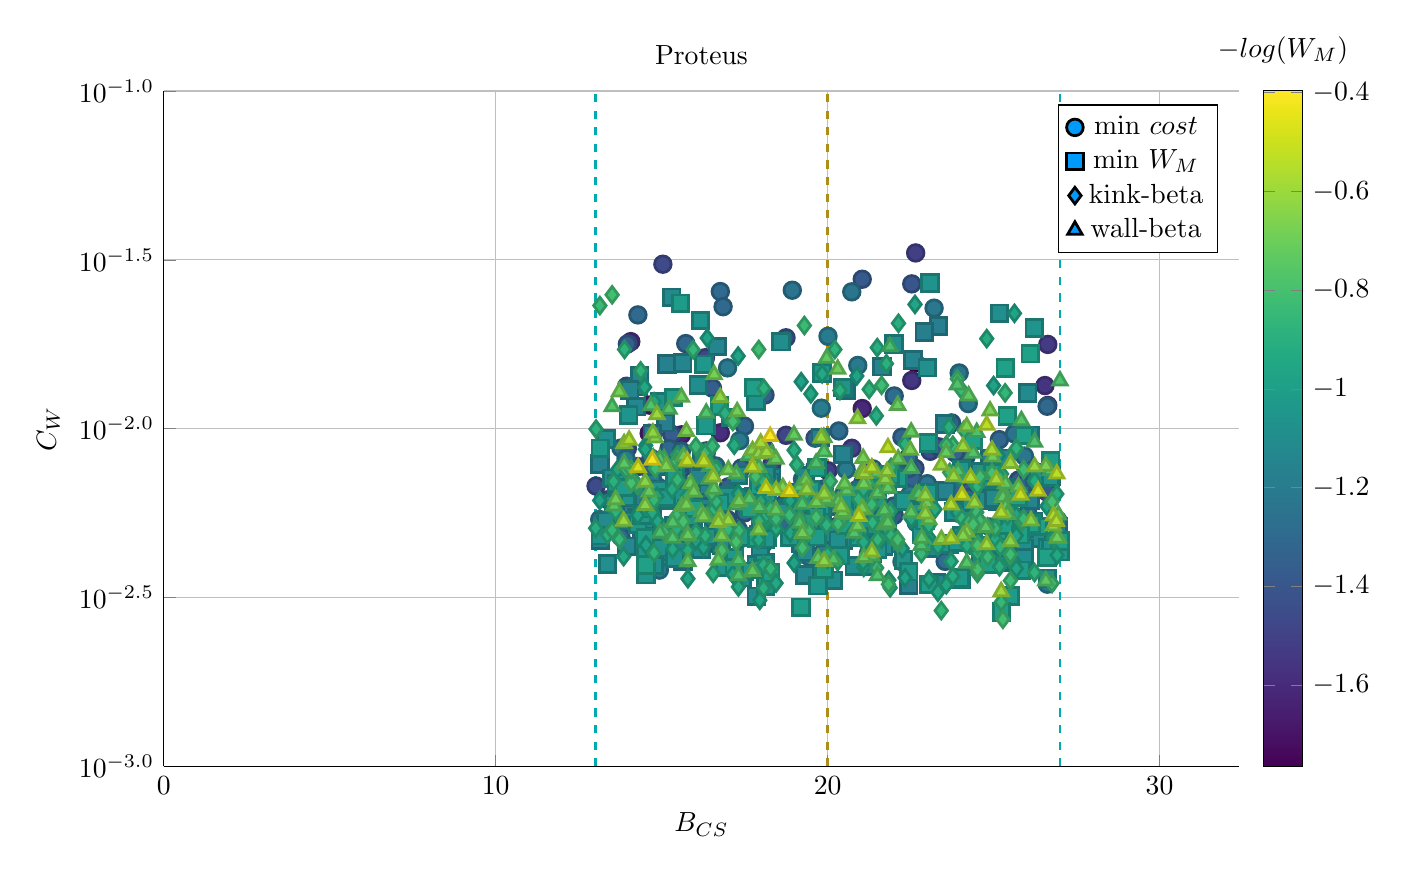
\begin{tikzpicture}[]
\begin{axis}[colorbar = {true}, height = {101.6mm}, ylabel = {${C}_{W}$}, title = {Proteus}, xmin = {0.0}, xmax = {32.398879571197455}, ymax = {0.1}, ymode = {log}, xlabel = {${B}_{CS}$}, {unbounded coords=jump, scaled x ticks = false, xticklabel style={rotate = 0}, xmajorgrids = true, xtick = {0.0,10.0,20.0,30.0}, xticklabels = {0,10,20,30}, xtick align = inside, axis lines* = left, scaled y ticks = false, yticklabel style={rotate = 0}, log basis y=10, ymajorgrids = true, ytick = {0.001,0.0031622776601683794,0.01,0.03162277660168379,0.1}, yticklabels = {$10^{-3.0}$,$10^{-2.5}$,$10^{-2.0}$,$10^{-1.5}$,$10^{-1.0}$}, ytick align = inside, axis lines* = left,     xshift = 0.0mm,
    yshift = 0.0mm,
    axis background/.style={fill={rgb,1:red,1.00000000;green,1.00000000;blue,1.00000000}}
, colormap={plots}{rgb=(0.26700400,0.00487400,0.32941500), rgb=(0.27794100,0.05632400,0.38119100), rgb=(0.28291000,0.10539300,0.42690200), rgb=(0.28229000,0.14591200,0.46151000), rgb=(0.27619400,0.19007400,0.49300100), rgb=(0.26514500,0.23295600,0.51659900), rgb=(0.25042500,0.27429000,0.53310300), rgb=(0.23360300,0.31382800,0.54391400), rgb=(0.21813000,0.34743200,0.55003800), rgb=(0.20123900,0.38367000,0.55429400), rgb=(0.18555600,0.41857000,0.55675300), rgb=(0.17117600,0.45253000,0.55796500), rgb=(0.15772900,0.48593200,0.55801300), rgb=(0.14618000,0.51541300,0.55682300), rgb=(0.13374300,0.54853500,0.55354100), rgb=(0.12346300,0.58168700,0.54744500), rgb=(0.11948300,0.61481700,0.53769200), rgb=(0.12632600,0.64410700,0.52531100), rgb=(0.15014800,0.67663100,0.50658900), rgb=(0.19109000,0.70836600,0.48228400), rgb=(0.24607000,0.73891000,0.45202400), rgb=(0.31192500,0.76782200,0.41558600), rgb=(0.37777900,0.79178100,0.37793900), rgb=(0.45867400,0.81636300,0.32972700), rgb=(0.54552400,0.83803900,0.27562600), rgb=(0.63690200,0.85654200,0.21662000), rgb=(0.73088900,0.87191600,0.15602900), rgb=(0.81457600,0.88339300,0.11034700), rgb=(0.90631100,0.89485500,0.09812500), rgb=(0.99324800,0.90615700,0.14393600)}, colorbar style={title=$-log( W_M )$}}, ymin = {0.001}, width = {152.4mm}]\addplot+[scatter, scatter src=explicit, only marks = {true}, color = {rgb,1:red,0.00000000;green,0.60560316;blue,0.97868012},
draw opacity=1,
line width=0,
solid,mark = *,
mark size = 3.0,
mark options = {
    color = {rgb,1:red,0.00000000;green,0.00000000;blue,0.00000000}, draw opacity = 1.0,
    fill = {rgb,1:red,0.00000000;green,0.60560316;blue,0.97868012}, fill opacity = 1,
    line width = 1,
    rotate = 0,
    solid
}] coordinates {
(22.651942134178245, 0.015650867313707448) [-1.7651507846396934]
(14.624587492471523, 0.009694646552347688) [-1.652530796858066]
(14.624587492471523, 0.011744038729478485) [-1.647000146345283]
(15.59515103457413, 0.009590177278586947) [-1.6184546481250472]
(21.041924335629172, 0.011474300333025303) [-1.6124908438767973]
(16.768060529085655, 0.00972401084478665) [-1.5828949402967583]
(14.070903864396604, 0.018106858351787505) [-1.577618500437912]
(26.63211955782928, 0.011719738653164523) [-1.56873554690934]
(26.54729756362062, 0.013419897432724169) [-1.5599002750009094]
(22.534449427914588, 0.013892471464509717) [-1.5518482038436605]
(26.63211955782928, 0.017767343192357253) [-1.5302287668791192]
(22.651942134178245, 0.033146306422516245) [-1.5115301730224102]
(20.011081752470886, 0.007510212646674021) [-1.5013825191439996]
(20.72766466016537, 0.008751202105526691) [-1.4958902811815062]
(15.146473848919625, 0.00816949735167802) [-1.4892617900728689]
(24.953221543185066, 0.008118078139228204) [-1.4884348201277007]
(18.74607790769805, 0.009559158760396884) [-1.4866425610729714]
(16.318569485171636, 0.01623184139531336) [-1.4835478223239928]
(18.31823242637104, 0.007837831837729894) [-1.4780728724015184]
(15.036815235314387, 0.03069401611625924) [-1.4650031348255397]
(13.023841119875671, 0.006765803188842749) [-1.4601242927308113]
(23.08827436791659, 0.008568870415676909) [-1.453691298071198]
(14.283963091120235, 0.007723927816166263) [-1.4489094778079963]
(13.382063426709323, 0.006162431971740805) [-1.432973868001932]
(18.11370115924847, 0.006329451983138475) [-1.4325147285303634]
(23.34059635854204, 0.008839617844718544) [-1.4268866569895065]
(13.967685136763796, 0.008744700190770928) [-1.4268347679685771]
(18.74607790769805, 0.018590297650719324) [-1.4237681445033143]
(16.531939570236105, 0.007587250291191641) [-1.4234658725845162]
(18.117461030315134, 0.007390656211515189) [-1.4109108269606008]
(18.117461030315134, 0.008694085637837138) [-1.4079262096010774]
(19.068604275965242, 0.00634066157530613) [-1.407330123320285]
(22.534449427914588, 0.026840973164111593) [-1.3996791570309395]
(25.747123007837175, 0.007040053838733538) [-1.3974870797438]
(13.944355842468203, 0.013359280479800206) [-1.3946269662443698]
(22.631885608490197, 0.007634837530984513) [-1.3905305073664083]
(26.612756674676874, 0.006488653571629467) [-1.3895960301339119]
(16.513096841535003, 0.00554611680879456) [-1.381931002288656]
(21.069685019437017, 0.00695131625200887) [-1.3818272949203658]
(21.041924335629172, 0.027704627448181397) [-1.3812563757949996]
(14.736556573901334, 0.00681167564679013) [-1.379699079550137]
(15.578926279356907, 0.006715817539753603) [-1.376650573885692]
(15.578926279356907, 0.00757067906104037) [-1.3758581110553065]
(24.170613812194496, 0.006499559071472007) [-1.375220700855124]
(23.73345635781125, 0.00646934556613389) [-1.3742348635950123]
(18.987744543833536, 0.0063267927368600325) [-1.3713423550361032]
(24.170613812194496, 0.008267480512087599) [-1.370057699317172]
(21.364079170448615, 0.004988896324536347) [-1.3686239973313072]
(22.006250519027304, 0.005540386026064644) [-1.3680076928767484]
(16.643751715736272, 0.005024205798518008) [-1.3672266212882762]
(15.300354897105095, 0.009628839399324697) [-1.3667105305870977]
(25.983749051053568, 0.0050592629231849704) [-1.3651176317240314]
(13.967685136763796, 0.017814080806893125) [-1.3612722200713383]
(15.565992883535738, 0.007840171434328094) [-1.360737823431438]
(16.531939570236105, 0.013182987051350502) [-1.3596008789905631]
(17.009377486662636, 0.006730765435871485) [-1.3568098625263256]
(17.49511712424178, 0.005632641769207446) [-1.3562925407270994]
(23.9635738853514, 0.005613911931897123) [-1.3540300242042478]
(20.336854083719853, 0.005176189759381431) [-1.3527684291391184]
(19.620614991884782, 0.007678792615766904) [-1.3513432280511455]
(25.983749051053568, 0.006888425944911811) [-1.3508742741062625]
(23.84218963638598, 0.006674090356682625) [-1.348444904526092]
(23.73345635781125, 0.010402669872398145) [-1.3482429808137002]
(19.620614991884782, 0.009376571407375644) [-1.3481015746033576]
(18.11370115924847, 0.012583797530216616) [-1.34746159692277]
(22.569231891000115, 0.007115527316776566) [-1.3450418873098828]
(24.492468867569784, 0.006464286011476574) [-1.3449397649071608]
(13.63676824165126, 0.006186516144095541) [-1.344834769873685]
(16.985654434835766, 0.0053864817732829605) [-1.3436955024234147]
(23.84218963638598, 0.00848434463520388) [-1.3426163725681677]
(15.156092946594729, 0.004938310227983135) [-1.3374912582230194]
(19.892081526120066, 0.006636608478826529) [-1.335539302100867]
(21.364079170448615, 0.007606581585076429) [-1.3352915983538123]
(14.277566761363651, 0.006029019944814239) [-1.331337874103357]
(16.34367742556589, 0.008594819258321628) [-1.3310780697195672]
(16.372753180241236, 0.004728216221281147) [-1.3292068036291638]
(18.651304149911, 0.005953363383436291) [-1.32828646244698]
(22.23750424468451, 0.009441137210103956) [-1.3280975618898123]
(14.816548429122673, 0.005079524630506098) [-1.3278697867431468]
(16.278758069854046, 0.005749625528658903) [-1.327757292865828]
(24.236502870832883, 0.006249734903697681) [-1.3253106415861637]
(21.376974447323292, 0.005155209960292018) [-1.3237407060184172]
(17.406035904117076, 0.007650804529712704) [-1.3217246458754282]
(16.676591700948407, 0.004926318213851794) [-1.319376268743699]
(20.218859975126456, 0.004774448071559269) [-1.3182101821558738]
(20.90842789138097, 0.0066268624262571275) [-1.31770129332637]
(15.726344083812931, 0.017867829271260238) [-1.3171626271127284]
(20.509174541398565, 0.006479743346210051) [-1.3144438328362922]
(17.49511712424178, 0.010177994071422254) [-1.314397397461996]
(25.17536025842546, 0.009279261565995508) [-1.3134452963620502]
(16.443823660899717, 0.005896178522672516) [-1.3126768401499638]
(21.376974447323292, 0.007223214696135702) [-1.3123916957087167]
(14.585638446869181, 0.007643344629724278) [-1.3117090270675453]
(14.29222630999366, 0.0062843154751196315) [-1.3112976001573549]
(19.34016378549167, 0.006316305209750007) [-1.3102933400586538]
(26.612756674676874, 0.011655743235665423) [-1.3084666426112759]
(14.677311567391737, 0.008181643780093392) [-1.3081739820914746]
(23.930583881480565, 0.005920113041607297) [-1.3081169022767745]
(18.59998810930447, 0.005266304291939928) [-1.3075986397555424]
(21.639804877968437, 0.0056632699287416785) [-1.3038897119548887]
(14.341073675298674, 0.004515583648974614) [-1.3034916079905217]
(22.44852739031052, 0.00762405310841983) [-1.301506470226052]
(14.283963091120235, 0.021723513711501174) [-1.2978787946122285]
(23.797921766937304, 0.005860560202229156) [-1.297460949292816]
(16.768060529085655, 0.02547444831481485) [-1.2953226778576867]
(16.850723243246257, 0.022974551007964673) [-1.2951062787178942]
(15.221638230176215, 0.008727794605170999) [-1.2946978796261759]
(21.194827607120533, 0.00606442154900928) [-1.293243062455323]
(13.773496878720852, 0.00478216163852665) [-1.2916316854649297]
(16.312384742623273, 0.004505685536187866) [-1.291573412415986]
(19.299286366301942, 0.006201757851874389) [-1.2910367642815292]
(14.715733335251208, 0.007056272547770033) [-1.2894268757747884]
(14.861104082210852, 0.004812007322004063) [-1.2891780169645117]
(21.99387616545991, 0.005900795309436559) [-1.2883016772579983]
(18.07568232599605, 0.004575860387174974) [-1.2877120777365891]
(16.5278219937302, 0.007501625869556503) [-1.2825608117529994]
(23.540570660663604, 0.004048206616482656) [-1.2803416949249293]
(22.006250519027304, 0.012501014524680899) [-1.2790944723531177]
(20.336854083719853, 0.009849033693022476) [-1.2789599032268324]
(21.229554500357366, 0.004266328381972482) [-1.278637308935949]
(14.019194247307421, 0.00602317781329061) [-1.2752962713941192]
(22.427243379042164, 0.008202673797589401) [-1.2724318730764337]
(19.80983944525114, 0.005313590913225172) [-1.26778944603233]
(15.630962235184002, 0.005746237915345085) [-1.2652894696394015]
(16.169659899199626, 0.0063394092295352205) [-1.263844406219344]
(19.370057307761773, 0.004670640784960837) [-1.2622412045786418]
(17.31176227830558, 0.005025369604276285) [-1.2622057750392766]
(17.350614255078973, 0.004715175023029078) [-1.2568407944078956]
(25.92926544649174, 0.005515822538041083) [-1.2564369672634057]
(13.773496878720852, 0.008763742702873716) [-1.255580803936347]
(19.24342166986986, 0.007090160917314494) [-1.2542825781236586]
(25.62853126166569, 0.009658252430988482) [-1.253606675738751]
(16.629549912781222, 0.005078101074449218) [-1.2533258835374417]
(21.331324879071882, 0.004668333949768413) [-1.252740293490489]
(26.02926384975561, 0.005623439530060779) [-1.2512906609771755]
(21.229554500357366, 0.007192663750971734) [-1.2505906665339703]
(26.93045024335227, 0.004753912504004936) [-1.2505667349102745]
(21.770706681119528, 0.00547669175115548) [-1.2505409706978425]
(15.59515103457413, 0.008585550973626429) [-1.2504311283223648]
(26.93045024335227, 0.00536142422310656) [-1.2495193060816674]
(22.748668314502247, 0.005891517799670805) [-1.2472203996667584]
(18.935691126914783, 0.025703839631456088) [-1.246340221801285]
(25.42163009914487, 0.004426672964739238) [-1.246337044553182]
(20.46656298748178, 0.004733745531528537) [-1.2444533586241864]
(19.245483292983383, 0.004373459187272198) [-1.2410504069560844]
(23.9635738853514, 0.014622918962551527) [-1.2404616678069278]
(20.72766466016537, 0.025422666134658947) [-1.2402101811954278]
(26.22602836680247, 0.00699405114862055) [-1.2399625556579728]
(19.15392842040434, 0.005459593535350185) [-1.2395775558220574]
(16.17194115370324, 0.006780135026174841) [-1.238968027160994]
(14.289259863079467, 0.006381273355008305) [-1.2381935518916032]
(19.245483292983383, 0.005454977773134567) [-1.2372164242860222]
(14.084051213081182, 0.006162937475975255) [-1.2359322527835273]
(25.92926544649174, 0.008295248979234676) [-1.2345953253761524]
(13.882021490725897, 0.005661235915534237) [-1.2333782101635051]
(24.89028576683355, 0.005116145429327062) [-1.2329256482335589]
(23.00100122686372, 0.0068738253515159406) [-1.2318041138227]
(16.629549912781222, 0.007759607253139788) [-1.2286780396839752]
(19.836396597287973, 0.004270512991179436) [-1.225800447150557]
(23.207115019583632, 0.022744869820021597) [-1.2237626122718148]
(17.350614255078973, 0.009221148903357415) [-1.2192315569877235]
(24.236502870832883, 0.011868028475244749) [-1.2191811590789894]
(16.34367742556589, 0.008481483201532794) [-1.2185680785343938]
(15.115258956268827, 0.00622802822970762) [-1.2179132583990178]
(14.90981948109104, 0.006703260233628488) [-1.2171472173843672]
(14.749136049291781, 0.00633213628058925) [-1.2167448502658762]
(20.90842789138097, 0.015392818825938645) [-1.2162995250149307]
(17.846164384152665, 0.003872910530196867) [-1.215703789534109]
(20.52604477006502, 0.004720977485089404) [-1.2156312790675603]
(22.124486957585535, 0.00736963569440644) [-1.2145283350978044]
(13.134678555839974, 0.005383150867826381) [-1.214317974252912]
(19.4366251326122, 0.004178935326843822) [-1.2138536176262873]
(26.62064413932083, 0.0034641548226198885) [-1.2119360055173332]
(14.931149108977916, 0.0038140534914709043) [-1.2104347246988538]
(20.557603047451465, 0.007570292211977012) [-1.2084631186053005]
(19.77593528714308, 0.0052385995930077645) [-1.2083264519217767]
(19.161909349795547, 0.005083028024589718) [-1.2073346872626274]
(22.23981527386949, 0.004039129704078142) [-1.2071975929322125]
(16.985654434835766, 0.01513911751066285) [-1.2067840670536927]
(22.486042313795984, 0.006395373245847939) [-1.206736577191552]
(26.236300999552455, 0.007483645463069493) [-1.2065799786199445]
(13.956526564952654, 0.005698374888186277) [-1.203843641047789]
(21.81360757918857, 0.005550896360654382) [-1.203724365314369]
(20.463153166774777, 0.005010777712400389) [-1.2024406864855146]
(14.715733335251208, 0.007157947201399507) [-1.2021169810907544]
(20.011081752470886, 0.01877759730610099) [-1.2015933815507112]
(14.00713301228089, 0.004489267037355289) [-1.2014423796656961]
(13.92658713143997, 0.006374667856956503) [-1.2011965112492808]
(14.486497670639796, 0.00572395742880883) [-1.2005427289121806]
(14.736556573901334, 0.0066192080125215165) [-1.1994215784439877]
(22.133490212694397, 0.007316062816603203) [-1.1975084180232178]
(19.80983944525114, 0.011502671870448664) [-1.1972619972446426]
(22.67137053609239, 0.005266662336518346) [-1.1967371969067386]
(26.735167824179122, 0.004368135902166705) [-1.1965134818457024]
(13.92658713143997, 0.008154332104698897) [-1.196084536648355]
(15.58476565413219, 0.006843978332329513) [-1.1943424204563022]
(25.30217158353333, 0.005029914775543452) [-1.1908054127888088]
};
\addlegendentry{min $cost$}
\addlegendentry{min $W_M$}
\addlegendentry{kink-beta}
\addlegendentry{wall-beta}
\addplot+[scatter, scatter src=explicit, only marks = {true}, color = {rgb,1:red,0.00000000;green,0.60560316;blue,0.97868012},
draw opacity=1,
line width=0,
solid,mark = square*,
mark size = 3.0,
mark options = {
    color = {rgb,1:red,0.00000000;green,0.00000000;blue,0.00000000}, draw opacity = 1.0,
    fill = {rgb,1:red,0.00000000;green,0.60560316;blue,0.97868012}, fill opacity = 1,
    line width = 1,
    rotate = 0,
    solid
}] coordinates {
(15.115258956268827, 0.010422279639263054) [-1.1890033537880158]
(14.715733335251208, 0.009658294464102987) [-1.1883675827161198]
(14.289259863079467, 0.013313745665171912) [-1.1879538738656286]
(19.892081526120066, 0.006487414571263668) [-1.1878029685724296]
(23.34059635854204, 0.020145877705477357) [-1.186260879134981]
(16.751068465480447, 0.005801884747670386) [-1.1859242026174677]
(20.313030948006798, 0.004217349677698315) [-1.183889066210908]
(20.08100946018568, 0.0058827996938258294) [-1.1830291222504283]
(24.89028576683355, 0.008160599297710009) [-1.1826268505607591]
(14.406348579120323, 0.004857174007518612) [-1.182365307189366]
(22.908762374221453, 0.01935279381255584) [-1.1822251925764147]
(20.278362500869783, 0.00447855648592392) [-1.1813612663460882]
(21.35046825241222, 0.00428725320402622) [-1.1785285195809967]
(15.6446694279654, 0.004053651772674214) [-1.1775655951090325]
(26.95198308809553, 0.005121496915389368) [-1.17705398157876]
(14.277566761363651, 0.005890819973806921) [-1.1767452937515073]
(25.12415251137596, 0.006104718148251412) [-1.1766083315756861]
(15.156092946594729, 0.01556268699280997) [-1.173888237216638]
(16.269054087414798, 0.005882961839613334) [-1.1734465174435744]
(20.278362500869783, 0.005961179911412564) [-1.1729466514857931]
(14.227206890976186, 0.006287276174883399) [-1.172839252676928]
(14.119035956708807, 0.005599267038542826) [-1.1727769211527406]
(26.11020939532839, 0.005070632392189801) [-1.1727372361954858]
(22.439521795398957, 0.003434292526080427) [-1.1726542785062386]
(17.248393366297435, 0.0062657093568900535) [-1.1703764252048678]
(16.5796794571122, 0.004942047034638912) [-1.1699166462753263]
(17.970910867302806, 0.004183590560340062) [-1.1681831393061217]
(16.624697426657203, 0.005170881199231806) [-1.1671080842733117]
(16.379855484535224, 0.006777996547666784) [-1.1655606692177785]
(20.463153166774777, 0.008402469668507205) [-1.165303541813206]
(13.151972673873539, 0.004666935296152095) [-1.1643973078802388]
(20.460136716993496, 0.004663766235492665) [-1.1632535008384055]
(19.2031189942159, 0.004566940606242733) [-1.1631989573193973]
(19.83550100861325, 0.0054331000812183365) [-1.1630392685982025]
(23.569327548205543, 0.006544368204474158) [-1.1625753891662707]
(13.671384109436172, 0.006511116933487475) [-1.1617936783337066]
(22.51827341524219, 0.006126048639979384) [-1.159367616011031]
(20.557603047451465, 0.012995381528200805) [-1.1593260324319568]
(18.135261940423753, 0.004013416769217783) [-1.1592024857112633]
(15.652603562708304, 0.004530529794416821) [-1.1590403977294572]
(13.139446789187307, 0.007867971330715704) [-1.1589428109110296]
(16.76328611632, 0.005330271588661515) [-1.158451320077056]
(14.857639167188884, 0.007724720119696045) [-1.157468772898154]
(24.758718787792066, 0.004436262085616985) [-1.1570637161067505]
(16.10076446545596, 0.007249642226094706) [-1.1563966451418943]
(19.77593528714308, 0.009420901412013665) [-1.1561531921827275]
(24.04992975868823, 0.0057898611640113395) [-1.1538328200442942]
(26.735167824179122, 0.007237376261288284) [-1.1525173430901554]
(17.092107947023983, 0.004881019954742076) [-1.1522162283529644]
(17.644214712877762, 0.0059379940430840635) [-1.151968932860403]
(26.108450807284747, 0.0061407721476487214) [-1.1511586507355254]
(21.639804877968437, 0.015255960449664327) [-1.1509834966159156]
(23.06727295287375, 0.004419080970160178) [-1.1503660387736743]
(23.540570660663604, 0.01032617135589161) [-1.1500086948877408]
(25.200810274108626, 0.004014883666259908) [-1.1494080253790357]
(19.32885457468507, 0.005291422749753008) [-1.1493093072503229]
(22.569231891000115, 0.01598351560152435) [-1.1489823622220707]
(21.074369777477393, 0.003915099463846501) [-1.1484511044037433]
(25.27069929453632, 0.005020529922825154) [-1.1483999797493492]
(23.27207804604334, 0.0034947010100993764) [-1.147064765638366]
(14.719150012234948, 0.005859550653426385) [-1.1465028274549764]
(24.247203750488318, 0.005641165149475234) [-1.144883586902141]
(18.31823242637104, 0.007176119328254024) [-1.144368544047569]
(16.20920986207578, 0.00802165691682325) [-1.1435280806157744]
(14.246324004196616, 0.005447269817044685) [-1.1433393449411435]
(25.35315185019304, 0.006668732693209443) [-1.143332108158641]
(19.971681515811508, 0.004886014774808058) [-1.143184585873657]
(16.676591700948407, 0.017515494611674454) [-1.1428249654095861]
(14.341073675298674, 0.014377117697389604) [-1.1427984862828113]
(14.040817864118065, 0.013005276311642224) [-1.142397010267489]
(21.194827607120533, 0.005929095379259443) [-1.1423708774410877]
(15.630962235184002, 0.01565086593371781) [-1.1422424769576425]
(19.32885457468507, 0.007266091038483963) [-1.140012696356206]
(20.5792220239773, 0.005840600330748377) [-1.1399465227440013]
(25.415403683525007, 0.00480284773560221) [-1.1387943392990294]
(19.654837660739332, 0.005752426766742318) [-1.1382802201938975]
(14.227206890976186, 0.011612930840038163) [-1.1380314198362265]
(19.150893512430507, 0.006446360072583165) [-1.137892443914052]
(26.11020939532839, 0.009562541252399106) [-1.1311113631375915]
(20.922532876081345, 0.005743536904522906) [-1.1302954325651586]
(24.59831707555059, 0.0041760314888273755) [-1.1295543261638465]
(14.802199219727623, 0.006161648966500728) [-1.129462828049983]
(19.31280667855182, 0.00369116854025651) [-1.1277963061708562]
(21.467959067562802, 0.006278926396423389) [-1.126807171194116]
(13.95165441994897, 0.004487529275565533) [-1.1267021554022474]
(18.269334848839954, 0.006938744439971839) [-1.1265761162904897]
(19.31280667855182, 0.004304336836767321) [-1.1261385034152473]
(15.968611966724305, 0.005917258047258142) [-1.1260458936236624]
(18.85019132037221, 0.005885263457738176) [-1.1250537668582923]
(14.486497670639796, 0.005616858230043609) [-1.124511019242948]
(17.9238683493206, 0.004843731890681865) [-1.1236988869720232]
(25.85696228036533, 0.005173923137495115) [-1.1235064786985465]
(19.860778911496865, 0.003624821435760545) [-1.1232730371267585]
(18.135261940423753, 0.007429853985811719) [-1.1231293548483412]
(14.36713722146902, 0.005231942783984398) [-1.1209978185544383]
(25.27069929453632, 0.008169617815892689) [-1.1196911148335087]
(24.792905974230315, 0.0061580609115664325) [-1.1194748634113345]
(14.94576539459215, 0.004188882178419093) [-1.119418152841014]
(17.83202655689412, 0.005791769416647159) [-1.1191123923650526]
(21.037434506959272, 0.004931972266091366) [-1.1181736482095217]
(16.33802128070243, 0.005611347227289511) [-1.1176702646643628]
(15.300354897105095, 0.024480989089009208) [-1.1175403888423328]
(16.804752354132532, 0.004518885765871233) [-1.1174827013795072]
(24.9997310960539, 0.0062233325455323925) [-1.1174414411464733]
(13.95165441994897, 0.006299808378708293) [-1.1171134960728113]
(21.91021863095728, 0.004568184715721437) [-1.1171111976535804]
(26.02926384975561, 0.012757776435747556) [-1.1168806186241906]
(18.159403641727735, 0.007305420869085463) [-1.1160945644374545]
(13.321210613736467, 0.005340773800773009) [-1.1139896885893594]
(17.421485223983048, 0.0036233885329560954) [-1.1123768792739945]
(26.198956758292148, 0.005311493039288053) [-1.1112153482766423]
(21.686800668420936, 0.0045000578497955725) [-1.1111283014916062]
(17.850925724336616, 0.003188662256079057) [-1.1108869662710774]
(19.233603569785046, 0.004842654136629077) [-1.1089922492653659]
(25.347291504394295, 0.00452032863173795) [-1.108391782497311]
(14.504420816138161, 0.00535669926333167) [-1.1082929384878708]
(26.32188665435516, 0.004745534590751309) [-1.1074346113685616]
(17.970910867302806, 0.004323464728471098) [-1.1074227437950106]
(17.30594937629188, 0.007293078759243216) [-1.1069130893453907]
(17.850925724336616, 0.003945456212149148) [-1.106325178133445]
(21.792402805381546, 0.004982808461571556) [-1.1060035644106432]
(17.970910867302806, 0.0052409052861536465) [-1.1038776732161713]
(21.069685019437017, 0.0065314531396132094) [-1.10351060592976]
(15.354808162096106, 0.005173060010686301) [-1.1022315889718237]
(17.92907707816459, 0.005951424789746293) [-1.1016702257969113]
(24.59831707555059, 0.007437806150470808) [-1.100448826904311]
(15.948854285961046, 0.005288339533793414) [-1.0998565094908217]
(14.961732146234509, 0.004337170224988449) [-1.0995498480529582]
(25.430993986088392, 0.005750254423520601) [-1.0992970719713648]
(25.92565373787029, 0.004423364554484401) [-1.0987351440216522]
(25.430993986088392, 0.006535275113176343) [-1.0983869460625248]
(21.792402805381546, 0.006822630998366228) [-1.0977261444257258]
(21.99387616545991, 0.017828562633364364) [-1.0969882385788774]
(16.191435661836504, 0.004407786879742766) [-1.096807077081938]
(25.920441712682297, 0.0041501216036249275) [-1.0962033310727437]
(13.367816836249185, 0.003972749736578854) [-1.0948458082881816]
(23.00100122686372, 0.015155543307471772) [-1.093965318294314]
(16.10076446545596, 0.013471957430229371) [-1.093275686079877]
(20.800547804595237, 0.003923510470624812) [-1.0931318196649105]
(18.59998810930447, 0.01811006730780237) [-1.0926393639694263]
(23.797921766937304, 0.005671433069083637) [-1.09199330517098]
(20.172158161026072, 0.0035546432563184145) [-1.0916603258728452]
(25.920441712682297, 0.005082501155756355) [-1.091508438458307]
(21.322964695317083, 0.003922207642532424) [-1.0911853630489914]
(13.508356065492707, 0.007129588907950501) [-1.0896526200520398]
(25.41312647977644, 0.004468466025444819) [-1.088663441639713]
(25.17536025842546, 0.021949864805969728) [-1.0877780715734315]
(13.321210613736467, 0.009322832924906896) [-1.0870739196827126]
(20.321218652713394, 0.004672088916974179) [-1.0855818982110972]
(17.197220657946232, 0.004039319528471343) [-1.0844715994400023]
(13.872957163284784, 0.0053439960085053) [-1.0842780595786392]
(22.748668314502247, 0.005760793758021615) [-1.084266572782003]
(21.108662110316036, 0.00569380985136289) [-1.0839928767281124]
(14.775761073278609, 0.0039349920083461085) [-1.0828594792618813]
(14.806549696522097, 0.0062405207423892875) [-1.082853352734588]
(18.145601806636947, 0.0054577800846403015) [-1.0824719035597]
(24.020772375357197, 0.0035809652689903063) [-1.0824709528228211]
(21.25065104433097, 0.005148297391297789) [-1.0814366033908964]
(15.662032516582798, 0.006582162000449632) [-1.0809878234039578]
(17.764718157329845, 0.006301853688415234) [-1.0808972954130593]
(17.421485223983048, 0.006161790226168522) [-1.0797863646031054]
(26.62064413932083, 0.0036086053477567665) [-1.079163153355685]
(16.368956330173987, 0.004793357206410555) [-1.0780309855478056]
(15.902251231898113, 0.0054298508521766365) [-1.076806285491668]
(19.34016378549167, 0.00604411217248383) [-1.0765985094568509]
(24.032420298396573, 0.004828662165485411) [-1.0760641298404754]
(18.651304149911, 0.005661819547798889) [-1.0757730303287785]
(26.62064413932083, 0.00443044659495794) [-1.0744056068515366]
(15.866386736192135, 0.005467468655559742) [-1.073726482715373]
(24.306579484746003, 0.006046667097602973) [-1.072815333291583]
(17.009377486662636, 0.006315687038558954) [-1.0718638391063322]
(14.931149108977916, 0.011989877345034696) [-1.0710072465261937]
(21.322964695317083, 0.006287200186056995) [-1.0706716976099708]
(26.32188665435516, 0.00739594343637032) [-1.069478881808043]
(17.846164384152665, 0.012080600310741674) [-1.0679830462657767]
(15.30993412600253, 0.006138341400017388) [-1.0670572282884458]
(22.284343035497017, 0.004085658341340117) [-1.0667391835901658]
(17.736283735115194, 0.006004004929014098) [-1.066302608545655]
(14.961732146234509, 0.004440975162005993) [-1.064104157833971]
(23.08827436791659, 0.026972932068461592) [-1.0640878812065675]
(21.508022779864863, 0.004395996587917252) [-1.0635820925869255]
(26.716640036139204, 0.004423420241739423) [-1.062988318250961]
(19.11527100708343, 0.00480727122317776) [-1.0628036997189863]
(18.131669417857122, 0.0034131330547271113) [-1.062700357913494]
(14.529712726466656, 0.0036974585830479817) [-1.0626514373993834]
(18.173944283111027, 0.004776499853086686) [-1.0610739421064752]
(15.401502456170876, 0.004144297606935685) [-1.0588352037418618]
(16.169659899199626, 0.0209014980088616) [-1.0585986545827941]
(14.00713301228089, 0.010988948677442597) [-1.057135771526312]
(20.46656298748178, 0.013241941603829825) [-1.056315661795303]
(26.22602836680247, 0.019862106250452566) [-1.0562734967702754]
(22.819346636869057, 0.004858658731965693) [-1.0561257856094448]
(19.11527100708343, 0.006223828461257365) [-1.0559814704124602]
(18.131669417857122, 0.004706089102701761) [-1.0555859489072712]
(18.079332919029085, 0.003994614402213268) [-1.0549803415205259]
(20.87914774430368, 0.006463993798881436) [-1.0545713902023608]
(16.908681604757444, 0.0038990516235787613) [-1.054205756099488]
(26.711777515939247, 0.007195479612398366) [-1.0536290024409787]
(13.929572546627387, 0.006286763322784177) [-1.0533216125601341]
(13.151972673873539, 0.004822724612666477) [-1.0529307720930816]
(22.819346636869057, 0.005656264568736301) [-1.0525850668019536]
(15.477350070944595, 0.006295530789348686) [-1.052552508886994]
(24.032420298396573, 0.007550888758433211) [-1.0509835312174363]
(15.45268981247694, 0.004904482654727138) [-1.0508250621973283]
(14.961732146234509, 0.006571304536184572) [-1.050680345054969]
(23.655268515644366, 0.004560195418506711) [-1.0506245233592775]
(17.092107947023983, 0.01080264515897382) [-1.0505217359121972]
(13.55338844221082, 0.00597835329976134) [-1.049317623712287]
(17.625908695494353, 0.00605275476812188) [-1.0490747591885061]
(24.537224497440306, 0.004511808104116367) [-1.0489907539423449]
(24.391233921325668, 0.0049153150140211965) [-1.0478434867034416]
(23.909126603799116, 0.004616652674773231) [-1.0473758850488442]
(18.173944283111027, 0.006447737760929581) [-1.046767629611379]
(22.284343035497017, 0.006114416229637186) [-1.0460742739305466]
(19.83550100861325, 0.01461141466329314) [-1.0428746875530057]
(19.710045895289856, 0.0034297894059699906) [-1.0409932776852704]
(26.99666218082735, 0.004324846597058025) [-1.040720375777512]
(13.63676824165126, 0.0068957525832947) [-1.0400494553390642]
(18.87182730714039, 0.0047742837106654985) [-1.03963800286999]
(24.953221543185066, 0.0070972253563865) [-1.0394862991533038]
(20.509174541398565, 0.006107051538135721) [-1.0391370640013136]
(16.278758069854046, 0.015503036624972183) [-1.038354289214968]
(23.035515049672192, 0.006445735380428859) [-1.0380750082543837]
(14.279438101093232, 0.005205902574339689) [-1.0370263081612092]
(21.737554950575895, 0.005283195240312258) [-1.0365321066837632]
(19.806577545472447, 0.005892181423629392) [-1.0364145571368009]
(16.33802128070243, 0.010214094301379546) [-1.0358730287795153]
(17.48698733172037, 0.003781581128188247) [-1.0352797650690977]
(21.495458720132525, 0.0061316127141858145) [-1.0352425491421158]
(14.518866161482416, 0.004345014451914255) [-1.0335536367675167]
(17.197220657946232, 0.00415632052734694) [-1.0319535365225938]
(15.134079464405815, 0.006253917955260214) [-1.031638330454266]
(23.993469701679754, 0.003613822408322808) [-1.0316283345953763]
(17.48698733172037, 0.00478160347928963) [-1.0312630056422283]
(24.747450186073678, 0.004326998549376461) [-1.030801418278412]
(16.751068465480447, 0.006039359373565179) [-1.0301227610636083]
(14.406348579120323, 0.005550817437725965) [-1.029015666765989]
(19.493426492317983, 0.006583295742064639) [-1.0288573869793878]
(20.37163275163815, 0.004204292638824563) [-1.0245024368116802]
(15.401502456170876, 0.007145400138218064) [-1.0231385619546913]
(19.68119459959854, 0.004789677204757558) [-1.021449027000752]
(17.924682632407837, 0.00675373673736514) [-1.0213127693885564]
(25.50482023490044, 0.003193542226257652) [-1.0209276741398987]
(22.124486957585535, 0.007121099635585821) [-1.0202684704954939]
(22.439521795398957, 0.0037708668397859442) [-1.0187837906200732]
(15.743591734002468, 0.005805595496214904) [-1.0179738483919518]
(23.035515049672192, 0.009070154520460257) [-1.0169425110693646]
(15.5630871969197, 0.00501503870041615) [-1.0162045101447212]
(13.869405436882781, 0.00670010251636303) [-1.0149810946438107]
(13.151972673873539, 0.008752580219573484) [-1.014353466976016]
(15.565992883535738, 0.023528952793841592) [-1.0140528730661398]
(19.665351838058136, 0.005527004085356763) [-1.0133093427968076]
(20.943775733817652, 0.004778958682375364) [-1.0128360857902137]
(18.033648098721542, 0.003842216867194081) [-1.0126834015105255]
(21.878860060352352, 0.007300503854095673) [-1.0124869131348806]
(25.83788180341901, 0.0038089628255598917) [-1.0084966915198963]
(26.716640036139204, 0.008048423371546378) [-1.005776006726422]
(26.339525393761082, 0.005136336479510988) [-1.0027757315503723]
(19.193829077288807, 0.0029594317443149176) [-1.002422823826331]
(23.0540274641531, 0.003459304695059543) [-1.0023352556688647]
(25.143925437510074, 0.004988217345842403) [-0.9994656987080655]
(26.999066309331212, 0.004649343635980374) [-0.9991953302395459]
(24.969602727169466, 0.007411548557741582) [-0.9991876183275935]
(17.18725041495652, 0.0038831217844692545) [-0.9971256954762724]
(25.239953702493796, 0.0028654321699102935) [-0.9968293366364798]
(24.38577334322156, 0.004992975570566671) [-0.9965130838642419]
(19.895557019888, 0.003830578946172306) [-0.9960911988132904]
(17.764718157329845, 0.013215773066776348) [-0.9953080727443692]
(22.937595078654155, 0.005338097758519931) [-0.994764309342816]
(14.62322740320338, 0.005798704578553127) [-0.9941918143808477]
(19.68119459959854, 0.007661762309327555) [-0.9939974184414383]
(15.354808162096106, 0.012372283627325148) [-0.9936895922796631]
(14.509582689075785, 0.0047417231470052315) [-0.9920762514365737]
(25.357682218729416, 0.005175409039233765) [-0.9891335090238219]
(17.644214712877762, 0.005799134035216279) [-0.988320863141931]
(24.822975077806525, 0.003975692742134705) [-0.9873980470532571]
(15.968611966724305, 0.005803966541873779) [-0.9872638091155089]
(19.372259092318934, 0.005281651647264406) [-0.9871243344745786]
(25.92565373787029, 0.00954881671016918) [-0.9862026242600886]
(24.391233921325668, 0.009231911938640338) [-0.9851939256634008]
(26.125739860092395, 0.005233428706224578) [-0.9845137991026185]
(25.35315185019304, 0.015110407509335635) [-0.9844063088607684]
(25.747123007837175, 0.006274740712107015) [-0.9843851675543582]
(26.108450807284747, 0.01666579340898781) [-0.9832677624207663]
(17.860630065422363, 0.004743145828135927) [-0.9823156156623659]
(18.28268228926236, 0.003744148435661381) [-0.9817957805945331]
(25.812435546384016, 0.0048552692105239565) [-0.9817262777133879]
(16.751068465480447, 0.01167873981501713) [-0.980944500204026]
(26.605009277171177, 0.004161496814710868) [-0.9808435285359967]
(25.41312647977644, 0.010903168023481107) [-0.9803069086017846]
(20.536092995679923, 0.005187973951951495) [-0.979926239566149]
(14.529712726466656, 0.0039527765780552285) [-0.9799255860420428]
};
\addlegendentry{min $cost$}
\addlegendentry{min $W_M$}
\addlegendentry{kink-beta}
\addlegendentry{wall-beta}
\addplot+[scatter, scatter src=explicit, only marks = {true}, color = {rgb,1:red,0.00000000;green,0.60560316;blue,0.97868012},
draw opacity=1,
line width=0,
solid,mark = diamond*,
mark size = 3.0,
mark options = {
    color = {rgb,1:red,0.00000000;green,0.00000000;blue,0.00000000}, draw opacity = 1.0,
    fill = {rgb,1:red,0.00000000;green,0.60560316;blue,0.97868012}, fill opacity = 1,
    line width = 1,
    rotate = 0,
    solid
}] coordinates {
(21.711893029131566, 0.0049343734079309275) [-0.9797193514246809]
(20.87914774430368, 0.014326928101993836) [-0.9793649258547107]
(22.249101100040285, 0.004418560150536774) [-0.9793554194238832]
(23.993469701679754, 0.007133046942930264) [-0.9793399260652301]
(14.529712726466656, 0.004527202123528333) [-0.9786718824413932]
(19.2031189942159, 0.013777079521683793) [-0.9784247640598123]
(25.079354543031585, 0.005278344797288595) [-0.9784156054323705]
(18.989026003231032, 0.004002965553163199) [-0.9772101816150688]
(24.9997310960539, 0.013418113026562503) [-0.9771245449599791]
(25.62847037709553, 0.004027289040267911) [-0.9768013676267739]
(16.372753180241236, 0.018551171796247393) [-0.9763993914483391]
(13.134678555839974, 0.006130885121857039) [-0.9762949474128021]
(16.427208297726143, 0.005562603331167774) [-0.9759999361809304]
(25.143925437510074, 0.008328856003390762) [-0.9748577786630778]
(19.99680496969866, 0.004109700372311695) [-0.9738966318394574]
(13.56697824167195, 0.004913914166672265) [-0.9734793512186626]
(16.03107337465876, 0.004665122126804512) [-0.9731032751395803]
(18.033648098721542, 0.006640697404806304) [-0.9726016535105552]
(24.427094392002633, 0.004736078134325021) [-0.9724572780741577]
(23.908352016960492, 0.005647304198937851) [-0.9722087723669882]
(24.79132961055872, 0.004389286248628818) [-0.9718244022964762]
(22.332295899617375, 0.0036192646662402627) [-0.970582002945255]
(13.671384109436172, 0.007574170243236733) [-0.9693863160362324]
(17.30594937629188, 0.016406094197261946) [-0.968978562403945]
(18.87182730714039, 0.004910644527520683) [-0.9682987091511867]
(21.62636840883897, 0.004713875842941002) [-0.9661896439247507]
(19.193829077288807, 0.005899389733384474) [-0.96458538139874]
(21.793166599979934, 0.0056286885015633895) [-0.9644132418595727]
(16.260430864278227, 0.004458328702018249) [-0.9642494738631832]
(26.605009277171177, 0.005896947846453336) [-0.9638749980488863]
(14.518866161482416, 0.008919099387898428) [-0.9633607889353855]
(17.144948028029052, 0.003704995647544644) [-0.9628913890413714]
(18.87182730714039, 0.00612171997200749) [-0.9627420883815555]
(21.843108678301228, 0.003560196433315863) [-0.9623524414535783]
(25.62853126166569, 0.02195538724653361) [-0.9620751879990892]
(17.955918213319755, 0.0031037314795763953) [-0.9616273380898692]
(23.06727295287375, 0.004737846584498155) [-0.9614728013262]
(22.9924640163578, 0.0056288454988440186) [-0.9611621976310423]
(17.31176227830558, 0.006420794710655912) [-0.9607076853432408]
(25.68282437564652, 0.004827398822111102) [-0.9600064809118957]
(22.631885608490197, 0.02333271298987377) [-0.9582788764682687]
(25.68282437564652, 0.005548252171458194) [-0.9582126253448857]
(23.06727295287375, 0.005664193052715976) [-0.9580357625022031]
(14.279438101093232, 0.005536719771654066) [-0.957784719926681]
(25.68559192901304, 0.003853864382102105) [-0.9569481934101607]
(16.556270886342375, 0.005755412847229535) [-0.9553125817248839]
(14.509582689075785, 0.008689466677368552) [-0.9542931196842905]
(16.58107133568487, 0.0059335279307082415) [-0.9535689234008579]
(22.517026888269854, 0.00540418577910244) [-0.9533577705177119]
(20.77275422833572, 0.004951751523060612) [-0.9524896594035642]
(15.790739414166003, 0.0035965091424978767) [-0.9519498604980341]
(16.804752354132532, 0.005225320910765454) [-0.9518141933322811]
(21.467959067562802, 0.0064487141747247515) [-0.9516817791582881]
(26.80433260075194, 0.004824944888873151) [-0.9503280372896984]
(24.08056889459325, 0.00494548994415281) [-0.9501901690400224]
(14.861104082210852, 0.005348280279251544) [-0.9501200807106565]
(23.575238252030694, 0.003451161099821506) [-0.9494094470373718]
(19.493426492317983, 0.012679296138241048) [-0.9485432404545778]
(14.861104082210852, 0.006306624155522614) [-0.9476409244484506]
(14.486497670639796, 0.013277570668597095) [-0.945668217439486]
(14.775761073278609, 0.012011087422302516) [-0.9455646191283261]
(26.913506127016916, 0.0042225651663969944) [-0.9452539976263535]
(21.817575837477094, 0.007400046119087899) [-0.9445379968061569]
(21.088494147417737, 0.0038853521635503845) [-0.9442842771351952]
(23.0540274641531, 0.003581425300578328) [-0.9439633256599537]
(19.836396597287973, 0.014533706969027229) [-0.9435190061725043]
(21.495170330924516, 0.005251128867230356) [-0.9431579759120018]
(23.32241055960176, 0.0032803092315458883) [-0.9428483368499935]
(16.76328611632, 0.005138967929828396) [-0.9422331530579936]
(18.447686620108747, 0.0034905159514662587) [-0.9396609276523904]
(21.074369777477393, 0.004029446318551389) [-0.939623008122614]
(23.0540274641531, 0.00455015926208741) [-0.9389137302612279]
(15.33021544852462, 0.00439803335731196) [-0.938282475354221]
(18.159403641727735, 0.007076676002554203) [-0.9381610470878076]
(13.855662151001413, 0.004180164094848145) [-0.9375089447207223]
(25.047879452913545, 0.0047224227678250175) [-0.9369328543779993]
(17.98391484948191, 0.0060949751266714085) [-0.9362670591806482]
(14.719150012234948, 0.005648330019282998) [-0.9352069487820426]
(24.387769811025546, 0.005000154489324483) [-0.9348472459577944]
(17.955918213319755, 0.005297957377087851) [-0.9342522553820941]
(21.495170330924516, 0.006759629185969791) [-0.9338432220939059]
(15.30993412600253, 0.006608248212098614) [-0.9331696663167082]
(23.32241055960176, 0.004476157560195598) [-0.9323821674335669]
(22.834131439170747, 0.004553679627799357) [-0.9312147370194936]
(24.537224497440306, 0.004658130964295737) [-0.930280167995953]
(18.447686620108747, 0.005060711761627857) [-0.9280045677807334]
(24.792905974230315, 0.018476285473848813) [-0.9280031254185547]
(17.312868144499753, 0.0034004941489706427) [-0.9276368843131759]
(24.59404027903679, 0.005166624841841688) [-0.9268239261037757]
(15.785946454503529, 0.004359745755123362) [-0.926124917347277]
(23.23495821442244, 0.005775582114052551) [-0.9257073204007308]
(17.18725041495652, 0.008935057639573897) [-0.924623493423007]
(19.158825560243013, 0.005284834073095107) [-0.9243237059537647]
(24.387769811025546, 0.006960808141066332) [-0.9233834598837832]
(24.764249505652145, 0.004477816754705252) [-0.9228152651263011]
(15.610110935591706, 0.005256266572834143) [-0.9225398322566478]
(21.086014975073198, 0.004614605578452094) [-0.9221817845745035]
(17.9238683493206, 0.004684328138894626) [-0.9215264386089611]
(13.011374727983977, 0.005073667236310502) [-0.9182360577808578]
(26.236300999552455, 0.00699448652183368) [-0.9171606639000199]
(25.496539583465434, 0.004096269252840535) [-0.9167994991962954]
(24.105981493227365, 0.004877105036737716) [-0.9148199077007076]
(18.145601806636947, 0.005333658362398189) [-0.9143950266851926]
(15.772215710533262, 0.0063326000908344015) [-0.9137204603649657]
(23.77209082045688, 0.003656199076187517) [-0.9133127453951064]
(26.905013263566943, 0.006406059775809559) [-0.9121627392578615]
(21.843108678301228, 0.006847766811629225) [-0.9120709030515949]
(21.074369777477393, 0.006587871594639965) [-0.9120475096142877]
(24.537224497440306, 0.006957117514637042) [-0.9120417957644669]
(21.88346447009828, 0.003379934383470047) [-0.9119544487627024]
(21.467959067562802, 0.010913194864582846) [-0.911708891151293]
(20.30332931675502, 0.004041226194685478) [-0.9111798161472054]
(25.239953702493796, 0.0073486956507704685) [-0.9107411837742436]
(26.79882485524314, 0.004735506056694406) [-0.9100560207797687]
(23.655268515644366, 0.010112207946458425) [-0.9096645202732524]
(18.989026003231032, 0.008635225183072814) [-0.9087883894803973]
(21.686800668420936, 0.005403661462545021) [-0.9082790009204854]
(23.71920555338414, 0.004047054134608013) [-0.9081431792626627]
(25.17696423356227, 0.003902974011235298) [-0.9067699437470415]
(21.495458720132525, 0.017382642208156447) [-0.9060971962820227]
(24.194837362132866, 0.004507017121233361) [-0.9060048430542386]
(18.442422810906905, 0.0054677225459759575) [-0.9051444524245076]
(19.99680496969866, 0.004250447610661418) [-0.9046954309394458]
(25.42163009914487, 0.005523706134151735) [-0.9046460109599029]
(15.469368499099941, 0.005058679669540388) [-0.9046042329773717]
(19.15808110804699, 0.004880341290688154) [-0.9039977279126346]
(13.367816836249185, 0.004848014991264962) [-0.9034337968845987]
(18.072238642477593, 0.0033710581928259836) [-0.9031566859943262]
(22.133490212694397, 0.02051608060889296) [-0.9023267465363606]
(18.072238642477593, 0.00394866132787808) [-0.9008355008980751]
(16.908681604757444, 0.011116102682336754) [-0.9007285357561787]
(16.552565712961382, 0.0037301270643077876) [-0.8972742280672815]
(13.55338844221082, 0.006975150409970039) [-0.897175036870542]
(24.511261732188537, 0.004282665596744035) [-0.8971186814881362]
(20.37163275163815, 0.012972814791692319) [-0.8969796612342156]
(23.05056195453426, 0.0051618357133361315) [-0.89672282177903]
(21.770706681119528, 0.015575744813995764) [-0.8963952627105445]
(18.269334848839954, 0.006658522954563811) [-0.8958485488547734]
(18.07568232599605, 0.005404120857058153) [-0.8943684288096996]
(22.332295899617375, 0.009007603010797853) [-0.8914082601651864]
(18.07568232599605, 0.006944169371814818) [-0.8896483571913044]
(19.99680496969866, 0.006491642132230442) [-0.8869865112217631]
(13.023841119875671, 0.009974107942199384) [-0.8866075677924622]
(18.079332919029085, 0.013162396177814029) [-0.8851823316418669]
(21.91021863095728, 0.004826124490303322) [-0.8846740900795415]
(13.616480154545364, 0.005684202227253982) [-0.8840192815000373]
(16.312384742623273, 0.0048201007942522064) [-0.8839767416908659]
(19.068604275965242, 0.007830361841197038) [-0.8835453569153728]
(19.968999576205356, 0.005186138093663713) [-0.8832514898254401]
(17.93627510472957, 0.0053254692875210185) [-0.8832295476215102]
(25.62847037709553, 0.008573190683116311) [-0.883069564455261]
(25.200810274108626, 0.004462559243137306) [-0.8830632191913902]
(21.88346447009828, 0.005696949886972815) [-0.8825797897872378]
(13.882021490725897, 0.01716789737474233) [-0.8801231316414504]
(21.35046825241222, 0.005269633409728344) [-0.8791867595932125]
(20.922532876081345, 0.006190708259408953) [-0.877951083604425]
(21.25065104433097, 0.013073202281995273) [-0.8774262288873376]
(15.902251231898113, 0.006886241915548495) [-0.8751523935645794]
(26.232326861807465, 0.003750268079957199) [-0.8748921304141444]
(14.36713722146902, 0.014828542032509849) [-0.874690516784764]
(14.771138015954458, 0.004289107281658671) [-0.8742887892359985]
(16.58107133568487, 0.005786133363621624) [-0.8739921539442262]
(25.68559192901304, 0.008747322528766296) [-0.8716524887679293]
(20.218859975126456, 0.01715728174165555) [-0.8712831508374237]
(15.469368499099941, 0.008344053133431154) [-0.8707782727491976]
(24.511261732188537, 0.006756312980238707) [-0.8688158783682262]
(17.009893524049446, 0.005033506475358252) [-0.8686482360373176]
(16.643751715736272, 0.0060832943243140855) [-0.8685858440662988]
(16.03107337465876, 0.004920623586218273) [-0.8672784286683882]
(19.370057307761773, 0.004866417685086465) [-0.866786932045215]
(25.17696423356227, 0.007171410952306857) [-0.8662743883953999]
(21.508022779864863, 0.004690311648627596) [-0.8651646039969739]
(16.643751715736272, 0.007587597698564831) [-0.8649542416484729]
(16.20920986207578, 0.008493030870048135) [-0.8638854242016366]
(21.91021863095728, 0.007681026757569149) [-0.8637850725340939]
(18.28268228926236, 0.00385351424497451) [-0.8621520373035888]
(24.04992975868823, 0.005420954062013184) [-0.8611949292176813]
(25.347291504394295, 0.012767830297498842) [-0.8597568594294163]
(23.423616029838065, 0.0028935280651521448) [-0.859303050958753]
(15.477350070944595, 0.007054888627501927) [-0.85891018749718]
(13.508455039987684, 0.005004853345841743) [-0.8586165859116928]
(24.105981493227365, 0.009908479871966714) [-0.8586114389950454]
(14.771138015954458, 0.006151478093055551) [-0.8583221454358831]
(19.370057307761773, 0.006469455145345583) [-0.8577258338037467]
(24.247203750488318, 0.0052827318377912606) [-0.856994532353176]
(25.228628745964095, 0.0030638188926231558) [-0.8566075426873476]
(16.379855484535224, 0.008039114601071939) [-0.8562684441084778]
(15.948854285961046, 0.01712944125320649) [-0.8558052872802134]
(22.824087425680514, 0.004267584417782998) [-0.8545697779334551]
(16.312384742623273, 0.008482681890822595) [-0.8538958276429577]
(21.47813011726619, 0.003872739374790015) [-0.8535463695644936]
(16.5278219937302, 0.008873113176598642) [-0.85173359228685]
(25.047879452913545, 0.0050732777646726) [-0.8517054901788327]
(13.726047247124878, 0.004701607268823488) [-0.8493774101081241]
(19.158825560243013, 0.005419475274884782) [-0.8484701682854062]
(22.937595078654155, 0.00613724465859049) [-0.8467333432677736]
(13.929572546627387, 0.007557168723331712) [-0.8464349448005866]
(25.85696228036533, 0.005291739209830012) [-0.8453378253842451]
(17.331198319361267, 0.004983376401809511) [-0.8450087852753472]
(24.51457558642517, 0.003726820437409142) [-0.8448171197590391]
(18.28268228926236, 0.005789125924199343) [-0.8432574743352121]
(18.85019132037221, 0.005549754850410065) [-0.8430436771013377]
(14.277566761363651, 0.006783858344365182) [-0.8427718589011481]
(25.903908026071807, 0.005406145285483184) [-0.8415948084087838]
(18.448679664153556, 0.005406021522066206) [-0.8413272380615733]
(21.331324879071882, 0.005966658469646099) [-0.840505435392519]
(14.246324004196616, 0.006853609897202617) [-0.8403240064715908]
(20.409971582846815, 0.005315540207414598) [-0.8379028159133117]
(16.03107337465876, 0.008857688291635324) [-0.8377789816141492]
(14.90981948109104, 0.007938563015546142) [-0.8372578650925528]
(24.822975077806525, 0.004170239875860694) [-0.8369045170441011]
(24.492468867569784, 0.0056579135553807185) [-0.8359444642160421]
(23.77209082045688, 0.008931755340602409) [-0.8352235482527809]
(20.08100946018568, 0.006981447071324104) [-0.8348048184219272]
(26.75919220891685, 0.0034808725102794254) [-0.8343383061127448]
(13.139446789187307, 0.023150613766082406) [-0.833965424798725]
(24.020772375357197, 0.0130684108929944) [-0.8330108332095327]
(19.299286366301942, 0.02020816396851675) [-0.8328999767795251]
(24.822975077806525, 0.005117909063290362) [-0.8325894160918027]
(23.575238252030694, 0.008942904219591468) [-0.8305235366709506]
(24.59404027903679, 0.005329721235361873) [-0.8279917628427604]
(21.62636840883897, 0.013442707154089855) [-0.8257253077335049]
(19.4366251326122, 0.004961296668951894) [-0.8244439870918499]
(25.50482023490044, 0.003549416514808207) [-0.8243214968512095]
(15.070376902383966, 0.004936273572913412) [-0.8242933470610456]
(16.513096841535003, 0.006450216216685992) [-0.823012819256833]
(14.806549696522097, 0.0076278023903487095) [-0.8223450782723788]
(25.50482023490044, 0.004240662831829435) [-0.8222030505336514]
(22.113655252880513, 0.004583574206680189) [-0.8220930638276832]
(25.903908026071807, 0.007568987706711713) [-0.8220631016600264]
(15.45268981247694, 0.005518205902757275) [-0.8219864216086542]
(20.313030948006798, 0.005230785495605878) [-0.8219312934239001]
(23.908352016960492, 0.014042771210954628) [-0.8200917106540455]
(20.536092995679923, 0.0057025663921860025) [-0.8199389869999576]
(21.83179616436196, 0.003461216371181937) [-0.8184296236132867]
(24.59404027903679, 0.007217320297822837) [-0.8176734758564849]
(19.239362922333935, 0.004437347255537501) [-0.8154036160329199]
(17.924682632407837, 0.01716089273801921) [-0.8153527954342572]
(17.83202655689412, 0.007223735861818005) [-0.8144082854197419]
(17.144948028029052, 0.010504588562265854) [-0.8128175200037216]
(19.654837660739332, 0.005469791669344847) [-0.8124816458921246]
(15.45268981247694, 0.00800956789757918) [-0.811311819724745]
(13.508356065492707, 0.024915969416016464) [-0.8111026189728189]
(22.110321392556187, 0.004696885840713195) [-0.8093556032871382]
(23.676571204968464, 0.007424815290696485) [-0.8081403395005344]
(25.279679700751608, 0.002726446890806165) [-0.8078565007546591]
(19.886196105853493, 0.004060122004748655) [-0.8076401136101801]
(24.38577334322156, 0.00521133009673052) [-0.8058609898285525]
(15.652603562708304, 0.005311081041698119) [-0.8047538384635771]
(15.785946454503529, 0.004818293923541147) [-0.8045321061264834]
(26.75919220891685, 0.006080023629405084) [-0.804095594882759]
(14.084051213081182, 0.006910473351855834) [-0.8037221310081099]
(15.58476565413219, 0.008100775387463259) [-0.8035470296524466]
(14.084051213081182, 0.007575262106447099) [-0.8029316931085251]
(24.953221543185066, 0.007394228868903094) [-0.8027212756805284]
(24.51457558642517, 0.0038334779249383955) [-0.8021950738645045]
(17.24469713700245, 0.004623754785007905) [-0.8001182754285723]
(24.51457558642517, 0.004516682923706159) [-0.8000707725554996]
(16.807954356556944, 0.0043544029690039685) [-0.7981120109543962]
};
\addlegendentry{min $cost$}
\addlegendentry{min $W_M$}
\addlegendentry{kink-beta}
\addlegendentry{wall-beta}
\addplot+[scatter, scatter src=explicit, only marks = {true}, color = {rgb,1:red,0.00000000;green,0.60560316;blue,0.97868012},
draw opacity=1,
line width=0,
solid,mark = triangle*,
mark size = 3.0,
mark options = {
    color = {rgb,1:red,0.00000000;green,0.00000000;blue,0.00000000}, draw opacity = 1.0,
    fill = {rgb,1:red,0.00000000;green,0.60560316;blue,0.97868012}, fill opacity = 1,
    line width = 1,
    rotate = 0,
    solid
}] coordinates {
(21.878860060352352, 0.017490077363632575) [-0.796569715037787]
(21.194827607120533, 0.006971446105088665) [-0.79441004262747]
(14.94576539459215, 0.004911921812799429) [-0.7933559474809188]
(17.24469713700245, 0.005954017273857897) [-0.793170820712885]
(15.652603562708304, 0.007955591590128024) [-0.7930383455051904]
(19.654837660739332, 0.007901931985354861) [-0.7901570548309161]
(15.070376902383966, 0.008137353095022991) [-0.7899846868276869]
(22.824087425680514, 0.00451444584006381) [-0.7877812779595144]
(24.492468867569784, 0.009753587016237195) [-0.7866817518906072]
(21.50197112243447, 0.003671094509078405) [-0.7862115386558454]
(19.233603569785046, 0.005984919625817065) [-0.7857827687264937]
(16.443823660899717, 0.007731178757598179) [-0.7852361561866921]
(16.368956330173987, 0.005487637707476247) [-0.7839377375933054]
(17.312868144499753, 0.0036719603734188056) [-0.7819628551532836]
(19.15808110804699, 0.0052571395699657075) [-0.7811216845856691]
(26.999066309331212, 0.013864387522447816) [-0.7809918721633216]
(17.312868144499753, 0.004076457809715312) [-0.7809175837352759]
(23.909126603799116, 0.01348942620030939) [-0.7808076935800926]
(24.38577334322156, 0.008463888793993459) [-0.7806814861016669]
(23.930583881480565, 0.007481884358420134) [-0.7801570592845017]
(26.232326861807465, 0.009121533238626805) [-0.779570124080519]
(17.625908695494353, 0.008320597960456288) [-0.7795292440734509]
(18.31823242637104, 0.008435833537480966) [-0.7778143736900492]
(14.94576539459215, 0.008142288298726664) [-0.7773545006224067]
(21.83179616436196, 0.006689457230456803) [-0.7764899368885182]
(20.800547804595237, 0.0049083517753881175) [-0.7756195405244002]
(26.711777515939247, 0.007521529262855716) [-0.775153683924341]
(15.33021544852462, 0.004740003739998331) [-0.7750610829327748]
(19.15392842040434, 0.006724172004779728) [-0.7747436949495959]
(14.677311567391737, 0.011698217503304088) [-0.7742992479600759]
(22.67137053609239, 0.006405289888306118) [-0.7742009181502876]
(15.33021544852462, 0.005273402730059259) [-0.7740650517521674]
(21.47813011726619, 0.007399875727122566) [-0.7739873317108487]
(16.34367742556589, 0.01112021819603376) [-0.7725628696347435]
(20.172158161026072, 0.004092971739154845) [-0.7712605585908249]
(13.508455039987684, 0.011622544197713853) [-0.7710828598045486]
(17.93627510472957, 0.005847108178504653) [-0.7673997285740343]
(24.190608387466142, 0.004002837382643835) [-0.7673383740621305]
(22.748668314502247, 0.006406320488396418) [-0.7672456113797256]
(16.191435661836504, 0.005660698191622548) [-0.764435393058592]
(15.221638230176215, 0.011426609842125667) [-0.7638357297225782]
(22.51827341524219, 0.007631339242334709) [-0.7626015633802015]
(25.83788180341901, 0.01056591877280965) [-0.7619966091715842]
(16.427208297726143, 0.007093482393847056) [-0.7612576974946794]
(21.33239828922411, 0.004199528649097035) [-0.7606477643719728]
(20.172158161026072, 0.0061043171457404255) [-0.7605070169615751]
(13.56697824167195, 0.005910142488032306) [-0.758989724487738]
(17.644214712877762, 0.006191333042698553) [-0.7584940036454934]
(21.711893029131566, 0.005196318355535534) [-0.7578164289426172]
(21.711893029131566, 0.005719494012873511) [-0.7567591049966362]
(19.892081526120066, 0.008543926940425047) [-0.7538617973810071]
(17.248393366297435, 0.0073469528110748335) [-0.7537871731800888]
(21.50197112243447, 0.006441611010764987) [-0.7521304210847025]
(13.872957163284784, 0.007873808712793464) [-0.7505360316489605]
(14.749136049291781, 0.008186819140401449) [-0.7500694348357367]
(17.92907707816459, 0.0076761152805164415) [-0.7494357842274176]
(22.834131439170747, 0.0047411278954142926) [-0.7487383263348856]
(21.81360757918857, 0.005267487206516911) [-0.748295040109479]
(24.764249505652145, 0.00510155095748603) [-0.7479526703994891]
(20.321218652713394, 0.006094955162156969) [-0.7466544801447141]
(22.517026888269854, 0.005639377464652442) [-0.7463294557121921]
(20.5792220239773, 0.00656211934176063) [-0.7456515908681062]
(26.57397685761885, 0.0035438623842295783) [-0.7444648456519638]
(25.30217158353333, 0.006441345668266567) [-0.7439211998146191]
(25.279679700751608, 0.006262467782433261) [-0.7421222250103424]
(21.81360757918857, 0.0066746030671468205) [-0.7403121329507368]
(16.5796794571122, 0.006622183639274274) [-0.7387273173168031]
(24.247203750488318, 0.012518345047005714) [-0.7371532712992378]
(25.357682218729416, 0.00586330527207291) [-0.7360030908345161]
(20.52604477006502, 0.005573934279152215) [-0.7357478352131354]
(25.357682218729416, 0.006870018393163525) [-0.7339237337939822]
(17.73863700050444, 0.003781081009019496) [-0.7316156433190686]
(25.415403683525007, 0.005576715958847161) [-0.730702553629045]
(19.710045895289856, 0.004134252470600433) [-0.7303312511957366]
(19.968999576205356, 0.016171613473295127) [-0.729843436610322]
(15.790739414166003, 0.00404440687451383) [-0.729785410401758]
(26.95198308809553, 0.004753217414856202) [-0.7280136301997069]
(15.790739414166003, 0.004833924471763445) [-0.7277336612900158]
(21.086014975073198, 0.005768678984885649) [-0.7272359161193896]
(18.442422810906905, 0.00573908255056886) [-0.7261698897326505]
(19.971681515811508, 0.006183903992389591) [-0.7254945822919602]
(19.886196105853493, 0.009425592036620765) [-0.7248709166727003]
(16.706793066848114, 0.004083762847564463) [-0.7247250045744125]
(26.95198308809553, 0.00555669738244576) [-0.7243021962618132]
(14.62322740320338, 0.0065008956198242835) [-0.7231361773710641]
(18.987744543833536, 0.009573909711490997) [-0.7199601214619464]
(23.569327548205543, 0.008493769102557683) [-0.7192904335624307]
(21.088494147417737, 0.004161800763514465) [-0.7181717103320575]
(22.517026888269854, 0.009774432785564847) [-0.7157082647813301]
(25.747123007837175, 0.00672518720165279) [-0.7133538793997596]
(18.442422810906905, 0.008133758684308967) [-0.713147328980733]
(15.662032516582798, 0.008280513658244542) [-0.7119090304419833]
(22.9924640163578, 0.006015339197745989) [-0.711874379444345]
(19.34016378549167, 0.007033302783846991) [-0.7093738574733863]
(22.110321392556187, 0.011727088780751) [-0.7092628118222435]
(23.05056195453426, 0.005377543447438159) [-0.7082779809831496]
(22.124486957585535, 0.008128700004840336) [-0.7079149740331597]
(15.610110935591706, 0.0058863833594118755) [-0.7077375314316801]
(15.59515103457413, 0.012394108558435596) [-0.706334024208209]
(20.509174541398565, 0.006861678840585157) [-0.7060355945938097]
(15.866386736192135, 0.006864373636908622) [-0.7038135733626147]
(20.30332931675502, 0.015006249425988506) [-0.7037512219734932]
(20.460136716993496, 0.0056577722783176685) [-0.7035264465900107]
(26.913506127016916, 0.0047465607385720155) [-0.7022436655591267]
(19.239362922333935, 0.004898438903780831) [-0.7019504846768324]
(24.969602727169466, 0.008250562988123147) [-0.7016519102010582]
(15.968611966724305, 0.006496474197890071) [-0.7004682671343294]
(20.901135540071117, 0.005145205657743317) [-0.7004607417357811]
(21.088494147417737, 0.006854852769634591) [-0.697257876722007]
(19.665351838058136, 0.006051804862445387) [-0.6953271827789312]
(17.331198319361267, 0.006092815363031721) [-0.6948756488655455]
(15.743591734002468, 0.005948341687370322) [-0.6919725490450255]
(13.616480154545364, 0.0061691154576320574) [-0.6918216720826577]
(16.260430864278227, 0.0054945127517174305) [-0.6886003704823062]
(13.726047247124878, 0.012860214571413951) [-0.6865445113698354]
(17.274852976599064, 0.011227817940353334) [-0.6865379033167814]
(21.037434506959272, 0.005800308282021995) [-0.6863247651980258]
(17.009377486662636, 0.007550070260844876) [-0.6862505468129048]
(16.76328611632, 0.005486969125512323) [-0.6827724197832519]
(16.58107133568487, 0.014464387967398951) [-0.6824631897623205]
(21.037434506959272, 0.0074827989319399095) [-0.6818862739311917]
(16.807954356556944, 0.004806188895106216) [-0.681045803589209]
(21.069685019437017, 0.00816889826360917) [-0.676519673155459]
(22.486042313795984, 0.008648428702718012) [-0.6719661779681881]
(26.57397685761885, 0.007745025158563004) [-0.6704735841254407]
(24.894140788700845, 0.011288445943848816) [-0.6697397033471468]
(15.134079464405815, 0.007738022382834421) [-0.6679378664124311]
(17.9238683493206, 0.005015581678421179) [-0.664568252574071]
(18.651304149911, 0.00669592297226573) [-0.6634727256080692]
(15.743591734002468, 0.009819105400840689) [-0.6633739502994719]
(24.190608387466142, 0.010135569818090663) [-0.6603293996125943]
(14.802199219727623, 0.00939249858471365) [-0.65559527704335]
(24.194837362132866, 0.004941346717547644) [-0.6555295241521746]
(24.08056889459325, 0.004816500541784696) [-0.6547058060100277]
(20.409971582846815, 0.005870743901744645) [-0.6537537417688543]
(14.504420816138161, 0.005932794164922308) [-0.6464043889016696]
(14.504420816138161, 0.006947472050559312) [-0.6441524371503791]
(17.73863700050444, 0.008614150802832586) [-0.6435755088238163]
(25.507534342078195, 0.004628896988884589) [-0.6417612434876113]
(26.125739860092395, 0.005338370482502946) [-0.6411233744130039]
(23.427377594633388, 0.004699744627579453) [-0.640987214146381]
(21.737554950575895, 0.007087487092480624) [-0.6407246446539182]
(26.79882485524314, 0.00515820561993347) [-0.64043910323564]
(19.895557019888, 0.004048780696974486) [-0.6389038068208055]
(17.9238683493206, 0.00843149772202716) [-0.638861148766444]
(14.736556573901334, 0.009714499389582036) [-0.6294069795917682]
(19.372259092318934, 0.0066068889503494155) [-0.6275768971661828]
(22.94603564581136, 0.005596317067294422) [-0.6258147083581025]
(16.76328611632, 0.012383474644047428) [-0.6240811582101908]
(22.94603564581136, 0.006342206752876274) [-0.623858733293817]
(13.869405436882781, 0.009038977180576242) [-0.6219180031981787]
(19.895557019888, 0.006413229068552367) [-0.6211295209142411]
(20.901135540071117, 0.010716497136382792) [-0.6208626542170634]
(23.797921766937304, 0.007209680201685642) [-0.6167467450464242]
(21.793166599979934, 0.007474011503233748) [-0.6161668959029009]
(17.009893524049446, 0.005341623010745903) [-0.6158927687215917]
(24.427094392002633, 0.006034549350656402) [-0.6151171154024009]
(26.236300999552455, 0.007710534578292543) [-0.611487844722998]
(13.855662151001413, 0.005325687468973261) [-0.6105960450602266]
(19.806577545472447, 0.009395651952966138) [-0.6072970237328563]
(24.08056889459325, 0.008849998609604285) [-0.607167934756837]
(14.857639167188884, 0.011011436412354999) [-0.6068046108992835]
(23.427377594633388, 0.007800196444848983) [-0.6044115520464747]
(21.108662110316036, 0.0073754945362265924) [-0.6042994837220221]
(16.706793066848114, 0.005285659011122866) [-0.6039904096870199]
(24.79132961055872, 0.004536101420664817) [-0.6002259639912214]
(25.507534342078195, 0.007893069724651697) [-0.599628654709536]
(18.159403641727735, 0.008506562490937598) [-0.598984163230935]
(21.33239828922411, 0.004316469816027581) [-0.5959261626040724]
(16.556270886342375, 0.007203992072904583) [-0.5955950405014814]
(18.448679664153556, 0.006569799906212832) [-0.5938202025196627]
(25.228628745964095, 0.003293448348458264) [-0.5924965364478813]
(25.079354543031585, 0.0070697734857009835) [-0.5863105067137702]
(17.98391484948191, 0.009059683017711614) [-0.5857713266966416]
(24.94963630462124, 0.008641043968933318) [-0.5816462999976075]
(25.228628745964095, 0.005633523166219161) [-0.5704137695427589]
(14.019194247307421, 0.009253005496876103) [-0.5696437106298752]
(26.80433260075194, 0.005521854237443246) [-0.5674002220585073]
(23.71920555338414, 0.004724937285390053) [-0.5659611714323005]
(23.71920555338414, 0.005946042806037286) [-0.5624256589175691]
(26.890395392361725, 0.00531457081165648) [-0.5623603869588525]
(21.33239828922411, 0.007652522473212391) [-0.5622060582579881]
(24.306579484746003, 0.007158812168546282) [-0.5586016066139208]
(17.736283735115194, 0.007692772934772429) [-0.5432695620897464]
(16.269054087414798, 0.00799195574835828) [-0.5428363896952032]
(24.79132961055872, 0.010249112638021826) [-0.539430680583471]
(26.905013263566943, 0.007346405766288606) [-0.5383974392028681]
(21.817575837477094, 0.008784909565917896) [-0.5373180372652652]
(20.943775733817652, 0.0055030838414073325) [-0.5326220427069656]
(25.812435546384016, 0.006358422348850781) [-0.5205630703573453]
(15.772215710533262, 0.008016224358949506) [-0.5202460681153916]
(18.145601806636947, 0.006657238129354447) [-0.4996366974648138]
(24.04992975868823, 0.006356911553311087) [-0.4986461154825478]
(26.339525393761082, 0.006534404082035447) [-0.49130085436950693]
(14.29222630999366, 0.007673849676678937) [-0.47853240174435874]
(18.85019132037221, 0.006520797389370089) [-0.4429783531489627]
(14.719150012234948, 0.008070276950949126) [-0.4191253220081923]
(18.269334848839954, 0.00948755292374014) [-0.3962980847359198]
};
\addlegendentry{min $cost$}
\addlegendentry{min $W_M$}
\addlegendentry{kink-beta}
\addlegendentry{wall-beta}
\addplot+ [color = {rgb,1:red,0.00000048;green,0.66575898;blue,0.68099695},
draw opacity=1.0,
line width=1,
dashed,mark = none,
mark size = 2.0,
mark options = {
    color = {rgb,1:red,0.00000000;green,0.00000000;blue,0.00000000}, draw opacity = 1.0,
    fill = {rgb,1:red,0.00000048;green,0.66575898;blue,0.68099695}, fill opacity = 1.0,
    line width = 1,
    rotate = 0,
    solid
},forget plot]coordinates {
(13.0, 0.001)
(13.0, 0.1)
};
\addplot+ [color = {rgb,1:red,0.67554396;green,0.55566233;blue,0.09423434},
draw opacity=1.0,
line width=1,
dashed,mark = none,
mark size = 2.0,
mark options = {
    color = {rgb,1:red,0.00000000;green,0.00000000;blue,0.00000000}, draw opacity = 1.0,
    fill = {rgb,1:red,0.67554396;green,0.55566233;blue,0.09423434}, fill opacity = 1.0,
    line width = 1,
    rotate = 0,
    solid
},forget plot]coordinates {
(20.0, 0.001)
(20.0, 0.1)
};
\addplot+ [color = {rgb,1:red,0.00000048;green,0.66575898;blue,0.68099695},
draw opacity=1.0,
line width=1,
dashed,mark = none,
mark size = 2.0,
mark options = {
    color = {rgb,1:red,0.00000000;green,0.00000000;blue,0.00000000}, draw opacity = 1.0,
    fill = {rgb,1:red,0.00000048;green,0.66575898;blue,0.68099695}, fill opacity = 1.0,
    line width = 1,
    rotate = 0,
    solid
},forget plot]coordinates {
(27.0, 0.001)
(27.0, 0.1)
};
\end{axis}

\end{tikzpicture}

		\end{adjustbox}
        \caption{Proteus $B_{CS}$ Sampling}
    \end{subfigure}
    \hfill \hfill ~\\ ~\\ ~\\ ~\\
    \hfill 
    \begin{subfigure}[t]{0.45\textwidth}
        \centering
		\begin{adjustbox}{width=\textwidth}
			\Large
			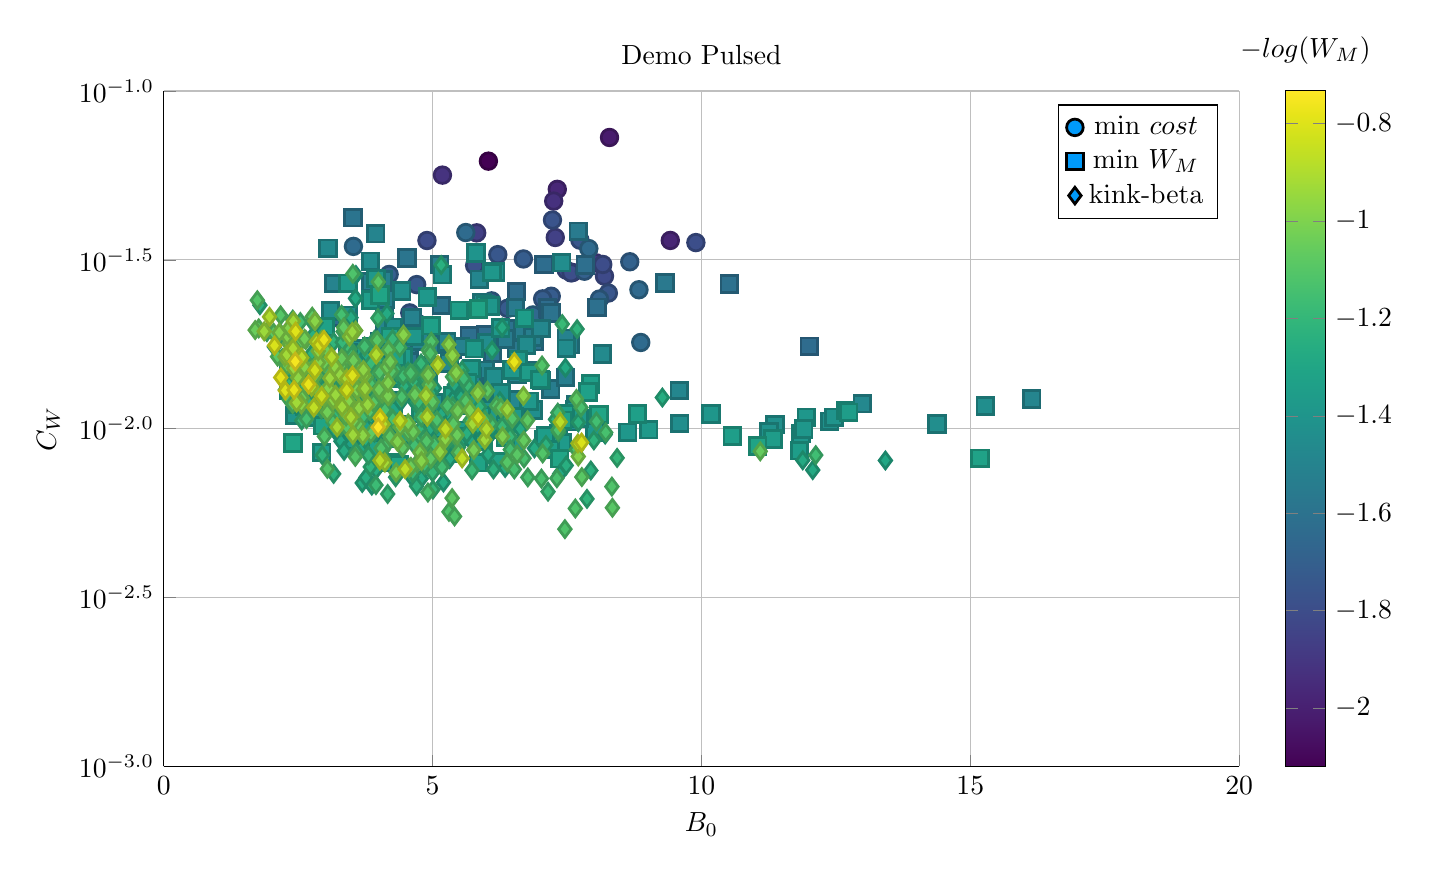
\begin{tikzpicture}[]
\begin{axis}[colorbar = {true}, height = {101.6mm}, ylabel = {${C}_{W}$}, title = {Demo Pulsed}, xmin = {0.0}, xmax = {20.0}, ymax = {0.1}, ymode = {log}, xlabel = {${B}_{0}$}, {unbounded coords=jump, scaled x ticks = false, xticklabel style={rotate = 0}, xmajorgrids = true, xtick = {0.0,5.0,10.0,15.0,20.0}, xticklabels = {0,5,10,15,20}, xtick align = inside, axis lines* = left, scaled y ticks = false, yticklabel style={rotate = 0}, log basis y=10, ymajorgrids = true, ytick = {0.001,0.0031622776601683794,0.01,0.03162277660168379,0.1}, yticklabels = {$10^{-3.0}$,$10^{-2.5}$,$10^{-2.0}$,$10^{-1.5}$,$10^{-1.0}$}, ytick align = inside, axis lines* = left,     xshift = 0.0mm,
    yshift = 0.0mm,
    axis background/.style={fill={rgb,1:red,1.00000000;green,1.00000000;blue,1.00000000}}
, colormap={plots}{rgb=(0.26700400,0.00487400,0.32941500), rgb=(0.27794100,0.05632400,0.38119100), rgb=(0.28291000,0.10539300,0.42690200), rgb=(0.28229000,0.14591200,0.46151000), rgb=(0.27619400,0.19007400,0.49300100), rgb=(0.26514500,0.23295600,0.51659900), rgb=(0.25042500,0.27429000,0.53310300), rgb=(0.23360300,0.31382800,0.54391400), rgb=(0.21813000,0.34743200,0.55003800), rgb=(0.20123900,0.38367000,0.55429400), rgb=(0.18555600,0.41857000,0.55675300), rgb=(0.17117600,0.45253000,0.55796500), rgb=(0.15772900,0.48593200,0.55801300), rgb=(0.14618000,0.51541300,0.55682300), rgb=(0.13374300,0.54853500,0.55354100), rgb=(0.12346300,0.58168700,0.54744500), rgb=(0.11948300,0.61481700,0.53769200), rgb=(0.12632600,0.64410700,0.52531100), rgb=(0.15014800,0.67663100,0.50658900), rgb=(0.19109000,0.70836600,0.48228400), rgb=(0.24607000,0.73891000,0.45202400), rgb=(0.31192500,0.76782200,0.41558600), rgb=(0.37777900,0.79178100,0.37793900), rgb=(0.45867400,0.81636300,0.32972700), rgb=(0.54552400,0.83803900,0.27562600), rgb=(0.63690200,0.85654200,0.21662000), rgb=(0.73088900,0.87191600,0.15602900), rgb=(0.81457600,0.88339300,0.11034700), rgb=(0.90631100,0.89485500,0.09812500), rgb=(0.99324800,0.90615700,0.14393600)}, colorbar style={title=$-log( W_M )$}}, ymin = {0.001}, width = {152.4mm}]\addplot+[scatter, scatter src=explicit, only marks = {true}, color = {rgb,1:red,0.00000000;green,0.60560316;blue,0.97868012},
draw opacity=1,
line width=0,
solid,mark = *,
mark size = 3.0,
mark options = {
    color = {rgb,1:red,0.00000000;green,0.00000000;blue,0.00000000}, draw opacity = 1.0,
    fill = {rgb,1:red,0.00000000;green,0.60560316;blue,0.97868012}, fill opacity = 1,
    line width = 1,
    rotate = 0,
    solid
}] coordinates {
(6.0376291897873084, 0.06197483174638786) [-2.119809409407475]
(8.29014098058992, 0.07282952610606806) [-2.022107373269494]
(9.420103794137964, 0.03609135913093006) [-1.9777667149411715]
(7.318722954994432, 0.051130362720294704) [-1.969913275543008]
(7.25219757869589, 0.047199699242522014) [-1.9276279243167613]
(5.1830212243548095, 0.05634035623848662) [-1.9180907603558137]
(7.605075373452645, 0.0290156978870517) [-1.8866814459155106]
(8.038027414173005, 0.030992141550921816) [-1.8810042714594786]
(5.819960412661949, 0.03801538835634297) [-1.861231108978198]
(7.281484484411212, 0.03683114347875789) [-1.8558362580925096]
(8.196367519793338, 0.028291519575269056) [-1.811508198071671]
(4.895214337316329, 0.03607745072820276) [-1.8048956433290855]
(8.164740419623248, 0.030644555029908985) [-1.797922304180305]
(7.485375190378305, 0.02949537628440487) [-1.7974494679074275]
(7.575835693873996, 0.028933124859920306) [-1.7961193741663348]
(9.896061646161176, 0.03557653455378664) [-1.7922955251500743]
(5.781753762991258, 0.030417392770278703) [-1.7763653379983415]
(7.2293817061271435, 0.04147970255534964) [-1.762574168304495]
(8.268196094729024, 0.025210912703269035) [-1.7524000959584443]
(7.738981336245074, 0.036173737778618126) [-1.7467043012053995]
(6.212564476265189, 0.032766263996239824) [-1.7445197156480476]
(4.575558741192934, 0.02202338694073385) [-1.7362913649987812]
(4.703832637956078, 0.026714074548194577) [-1.7340594740544224]
(6.392336735687798, 0.022713661122324157) [-1.7289223235866222]
(7.206811582654181, 0.02466928657304406) [-1.719614121069955]
(7.047211448521989, 0.024233508820652228) [-1.7167136137505041]
(6.688671457635685, 0.03181143352229567) [-1.7154437116459917]
(4.191978956537718, 0.028622291298276443) [-1.7060722509483957]
(7.823016295826839, 0.02926238447048653) [-1.6937830944780397]
(8.667006322370625, 0.03120868171359675) [-1.6889812321302553]
(6.097668524082785, 0.023905595143656186) [-1.686209077026567]
(8.103448360984764, 0.024204963735087338) [-1.6786883535604935]
(4.743339804248675, 0.020413682949498045) [-1.6734478593396724]
(6.86661111430788, 0.02171708878277083) [-1.650681965327452]
(8.837409416541565, 0.025789595420542006) [-1.6458495153344535]
(7.905189202860984, 0.034141771708853026) [-1.6412636709027566]
(5.617445394262159, 0.03809649700399676) [-1.6393314314904326]
(3.5279604177676442, 0.0346599142742729) [-1.6390302509540549]
(8.87108059531098, 0.018002375584230325) [-1.6381696948341165]
};
\addlegendentry{min $cost$}
\addlegendentry{min $W_M$}
\addlegendentry{kink-beta}
\addplot+[scatter, scatter src=explicit, only marks = {true}, color = {rgb,1:red,0.00000000;green,0.60560316;blue,0.97868012},
draw opacity=1,
line width=0,
solid,mark = square*,
mark size = 3.0,
mark options = {
    color = {rgb,1:red,0.00000000;green,0.00000000;blue,0.00000000}, draw opacity = 1.0,
    fill = {rgb,1:red,0.00000000;green,0.60560316;blue,0.97868012}, fill opacity = 1,
    line width = 1,
    rotate = 0,
    solid
}] coordinates {
(12.006327167234412, 0.017540808339758972) [-1.6348798048481208]
(7.13617498148303, 0.022785258097976623) [-1.6277277898588538]
(7.070736325233126, 0.030625514244526048) [-1.627684330571819]
(6.56017053121773, 0.025489957683783454) [-1.6248467182009472]
(5.980925581195891, 0.0189830433690413) [-1.62256122166559]
(5.681680569563924, 0.018838350678554387) [-1.6197529434592726]
(7.838353199376363, 0.030553347689269015) [-1.619473374550493]
(3.1599502425274832, 0.0213568595963161) [-1.6190205769362032]
(5.370255019403915, 0.017173711360022336) [-1.617478678707941]
(8.057787659408406, 0.022891816741403965) [-1.6135161817566324]
(10.515719243031652, 0.026834336105762403) [-1.6079101518459553]
(6.442976568556264, 0.01976733422078956) [-1.6005797137016178]
(6.892650960552643, 0.01811055755791537) [-1.5991182248913247]
(7.198509347079774, 0.02202289176749285) [-1.595836360479248]
(3.517726346433672, 0.042161103004000076) [-1.589397412964098]
(5.159769580238814, 0.0231728109038665) [-1.589205111302375]
(3.8365890735140322, 0.015450272567257462) [-1.5875377953010883]
(4.522678122476023, 0.0319953061173649) [-1.5845809864087244]
(4.56749863701147, 0.016164039710660088) [-1.5775674018565111]
(6.114630190971535, 0.016693759971981265) [-1.5713155071601692]
(6.555603899680141, 0.01726409176752251) [-1.5652457853616617]
(9.324368979144754, 0.02698353416604086) [-1.5643952661253622]
(4.546856339243231, 0.01769761001811183) [-1.5595601870169422]
(6.5407531731873325, 0.02281153437267921) [-1.552568848396255]
(7.709084001143297, 0.038423068705951594) [-1.5520441226990631]
(4.10568363851079, 0.022224095489930037) [-1.544925041354305]
(6.355103453558186, 0.01841847429182733) [-1.5430023738862098]
(6.679865116269665, 0.019477644457703495) [-1.5396243114452017]
(4.896210634322484, 0.01449908817629988) [-1.538692217528126]
(7.198003119281151, 0.013092644307368572) [-1.5373740781698282]
(5.131173117670862, 0.030574977212997605) [-1.5350312948909135]
(7.472740510067807, 0.014205258889817484) [-1.5317433014682034]
(6.8683725940871865, 0.018689708848548738) [-1.5311850486265117]
(5.766565183000099, 0.01387590038164943) [-1.5287451237254033]
(5.73965239781306, 0.013905952265261586) [-1.526526816139614]
(3.850247344392022, 0.027241135712482305) [-1.519178921439465]
(3.724681151757905, 0.016910779414334946) [-1.517891032933806]
(4.124143130105857, 0.024191852864153648) [-1.5130165343032327]
(7.561125230807454, 0.01773125993862434) [-1.5126055054907948]
(4.0802413603524945, 0.027530426264504002) [-1.5122759735909235]
(6.754598599599373, 0.014899481481132758) [-1.5121531835443067]
(5.140825889424527, 0.01778122202031051) [-1.5121518481580156]
(7.487694805484361, 0.01852162588841651) [-1.509963665969106]
(4.706543051446386, 0.013259386458548635) [-1.5098191352881933]
(4.023530685620901, 0.018078145365757758) [-1.5094600237705913]
(4.619206299311601, 0.02134336001409843) [-1.5091677016781566]
(5.515733266875538, 0.017507453096671365) [-1.505813383704145]
(3.1665229051711936, 0.026909424888676328) [-1.5035180904231982]
(4.7606297434625375, 0.018116695499993292) [-1.4998070828001184]
(2.6908911342489987, 0.01226652304303364) [-1.4993412700061268]
(5.9813285749518785, 0.014898889997617197) [-1.4970388348465338]
(5.73832856833363, 0.014279317114283529) [-1.4968151314329754]
(3.9410419383640107, 0.03778412752723575) [-1.4959262215207656]
(3.430490492055365, 0.012007443130458324) [-1.495878750102406]
(3.3992707879943804, 0.014131383104205364) [-1.4911760171512294]
(3.8869352833553514, 0.013847785437885679) [-1.4909012021072667]
(3.492353905872561, 0.013113327535403696) [-1.4904727997922445]
(16.140534236107158, 0.012253217681920671) [-1.4902975254497872]
(4.106645540108447, 0.020179920200301855) [-1.4899596862430686]
(6.569539440995961, 0.014465480638895564) [-1.484315053758591]
(9.588346294205625, 0.012974868808400592) [-1.4832272441818983]
(5.870682126151471, 0.02767164571202513) [-1.481908947186888]
(3.925275118526448, 0.012700241486954703) [-1.481610811848838]
(5.262489226894273, 0.018066556725317685) [-1.4808315890609627]
(5.861692393922073, 0.012152582495637852) [-1.4803924190961808]
(5.918313590579109, 0.023591043628319753) [-1.4777813991456452]
(3.8833429023200345, 0.014987126189756067) [-1.476226145125234]
(6.481366220083333, 0.012179602718049342) [-1.476103765156545]
(7.019026450980214, 0.0198044997246676) [-1.4759532635696884]
(12.992560883586702, 0.011854698849849837) [-1.4744693843941874]
(5.3126270403520905, 0.015665176708494814) [-1.4721189566530006]
(4.653270023129369, 0.012892988065699775) [-1.4694765884704042]
(5.56336817143885, 0.011723605612914264) [-1.4684762544315009]
(5.887370453127917, 0.01146148363735155) [-1.4673712598422484]
(4.769173324013478, 0.01403086783418577) [-1.4665127712450712]
(3.0555463671233567, 0.03422172209265897) [-1.466465342676487]
(7.658132277548963, 0.011814056076879775) [-1.4656409913573911]
(8.15735419014013, 0.01666169164744686) [-1.4607639902508311]
(3.6997605874700903, 0.011797068547740396) [-1.454804800167485]
(6.7465287199750925, 0.017714850999176746) [-1.454016548396377]
(7.488515154319888, 0.01730924236440855) [-1.449126660054787]
(4.899466318563284, 0.015350811156516968) [-1.4450317564339483]
(7.901350621283068, 0.010700521525178483) [-1.4442476160174416]
(6.002415704010382, 0.017999193081243068) [-1.4428695943470562]
(3.846424137063846, 0.03129913412451443) [-1.4416527786165851]
(7.401783272746636, 0.030992801350489627) [-1.4412978501823663]
(7.020304767734094, 0.013876797144792313) [-1.4410674847520173]
(14.381919368485658, 0.0103371343106061) [-1.4407593364531412]
(3.1028814474410384, 0.022291694526716137) [-1.4382523340904476]
(3.7705732972432857, 0.011033535668865918) [-1.4374618391296154]
(5.967712362691083, 0.011578760205733224) [-1.437309497392895]
(6.135496498952566, 0.014225493350487712) [-1.437004502630189]
(15.280361971651645, 0.011662685993065088) [-1.4369516286418977]
(9.595768152006077, 0.010363517857158673) [-1.4359296968945898]
(2.706516860566676, 0.012593943496598788) [-1.4348111698815942]
(7.531253395446069, 0.010486068251726523) [-1.4347403934029699]
(6.873696165627944, 0.011351647420548932) [-1.432162507533083]
(6.006312634325258, 0.010703895251080882) [-1.4298959659652046]
(11.369550336874795, 0.010279170294604838) [-1.429141349371285]
(4.426279201300683, 0.025557043779995653) [-1.4288294492620477]
(4.273188204709541, 0.019981046165081038) [-1.4275892047251812]
(3.284854781128933, 0.014011150106021747) [-1.42664672926539]
(3.563101077929043, 0.017276630179413652) [-1.4239039330716527]
(7.65153347612068, 0.01135063897630595) [-1.4237047673472223]
(3.427537242139707, 0.021651736693319764) [-1.4220880228019461]
(6.174362312871966, 0.029124606257697153) [-1.4214589216983458]
(12.38255150794347, 0.010524080735331771) [-1.4192750546166355]
(3.96419825273711, 0.012152497168515361) [-1.4188846212567885]
(4.984822443753677, 0.010654264771940928) [-1.418142111238707]
(4.177511278387798, 0.012093014306414056) [-1.4175771687309422]
(4.494983202230982, 0.010307835186267926) [-1.4166515403180218]
(11.258702848316975, 0.009802839106844477) [-1.4151591623618127]
(4.167168689552534, 0.012089411129630757) [-1.415086999740124]
(3.4268121903746978, 0.016771907819218872) [-1.4150518254702726]
(2.3537099631543916, 0.01479570625667246) [-1.412750376425469]
(5.182420388292304, 0.02858609969916251) [-1.4118418857799215]
(3.927997304454704, 0.009976658176736495) [-1.411745253778192]
(5.018593701573295, 0.011899859669740264) [-1.4101129990450592]
(3.885531120492574, 0.010975696046095008) [-1.4098064292280077]
(5.2474162565909435, 0.010078193568331789) [-1.4071217370506766]
(6.2004105061477235, 0.012567870805096065) [-1.4069653518342513]
(12.464033848113864, 0.010809590548122633) [-1.4053188021751997]
(3.762648000098064, 0.013228123351848638) [-1.4040831795581317]
(3.7635564019241006, 0.012756284815624411) [-1.403783408224447]
(6.2439977027647595, 0.011849909135487101) [-1.4034059706684434]
(4.011269493628918, 0.015391572104901911) [-1.4031334212883295]
(5.948372401188327, 0.011370525417095621) [-1.4027031557706915]
(6.105240096014571, 0.010883116023126084) [-1.4023409214316394]
(5.807785740293634, 0.03314304390232683) [-1.4018234466267534]
(6.240369813761391, 0.010943279854872806) [-1.4001967788421508]
(6.270554586884656, 0.012776602146795163) [-1.3983213447403338]
(10.178788051574003, 0.011065372696240975) [-1.3946316971345938]
(7.342798909437036, 0.009697674748088487) [-1.393981306323598]
(5.515659388841616, 0.012316212001497684) [-1.3939743444895971]
(5.981611630666005, 0.023293627402023516) [-1.3938659098694006]
(3.371060773893557, 0.012799262525216688) [-1.3934317035795]
(6.064709438936184, 0.02306752096780418) [-1.3919378361313393]
(2.855332574063217, 0.011575943181240602) [-1.3913501343623875]
(2.4437405695506387, 0.010938935413839007) [-1.3899986150261634]
(6.469695877217161, 0.014916276865219583) [-1.3888953225499234]
(11.950718647766315, 0.010811642128190005) [-1.3883849558567678]
(5.747775187553233, 0.012086573842968483) [-1.3880683151937296]
(8.62770676217042, 0.00974951527611275) [-1.3879257169733152]
(4.661434120932319, 0.01875474559032549) [-1.387200255154835]
(6.101706649362307, 0.028992717747430105) [-1.3869139374162498]
(4.921653466094031, 0.014275341697562267) [-1.385982080919773]
(11.85196051673142, 0.009658736241223327) [-1.385951966541943]
(11.902146743793873, 0.009979205376142167) [-1.384341496966052]
(8.017011891149473, 0.009781750047901397) [-1.3836628266676982]
(3.9453588859348705, 0.027837899406166513) [-1.383138617240496]
(2.7450573045264335, 0.013692957043690078) [-1.3831333668949872]
(6.793555399638037, 0.012055028195149642) [-1.3823755173012382]
(4.903012581972081, 0.02457168150365556) [-1.381386436684111]
(3.8233047461789904, 0.013467436970042478) [-1.381013926041926]
(3.9360749856112256, 0.01632900764605371) [-1.3807582017142732]
(4.3204944514848105, 0.016233342907168043) [-1.3795912650626003]
(6.26763114858317, 0.019856726760879642) [-1.3784744825946547]
(9.017994817618085, 0.009937020814786353) [-1.3784050115817357]
(5.662871931648498, 0.012947457233964572) [-1.3727350903904059]
(3.423561741004342, 0.02692798924274793) [-1.3726382795387042]
(6.527451391525709, 0.00894061047284123) [-1.3726183217257064]
(6.511799045245276, 0.01083618948017438) [-1.370506635821487]
(6.061861020595905, 0.010820381028973857) [-1.3702834841058706]
(5.720454003557526, 0.01507474130083674) [-1.3699905172740252]
(6.595551058907596, 0.016024901755414496) [-1.3694510931398833]
(7.0656961487120595, 0.009286958803152093) [-1.3690194932725448]
(5.7756989121996005, 0.01725165686414962) [-1.3685993689556193]
(7.407124185747266, 0.009100422809121853) [-1.3680782620249432]
(5.940087524048422, 0.009358898748733285) [-1.3659937757563743]
(7.721929512311208, 0.010741593794976297) [-1.3655266043175585]
(4.375024347794328, 0.00935804014953258) [-1.365489135635999]
(4.45788760453061, 0.01631624677926724) [-1.365314944668722]
(12.678530079731434, 0.011316654652064283) [-1.3620488306806053]
(2.8403626573133516, 0.010811158792461435) [-1.3600883836878876]
(6.791476575808721, 0.014663988794896813) [-1.3569999482959285]
(11.332959766691456, 0.009327975573933072) [-1.3565369493574833]
(3.5993697558328135, 0.009591330831744169) [-1.3564434514013937]
(7.094333669876596, 0.009510520762087537) [-1.355670949654743]
(11.824184374151493, 0.008600603815848054) [-1.3550689180362785]
(6.708017904184935, 0.0212306523206366) [-1.3545717493575382]
(3.9462715514882833, 0.011027495783414606) [-1.3536406793714741]
(3.846707059253749, 0.02403578580290836) [-1.3522480304376618]
(5.54278675314685, 0.01277987363566607) [-1.351683168790268]
(12.739777598462709, 0.011181317227288103) [-1.3509416538039447]
(6.996720111065061, 0.013988110662625983) [-1.350917699634303]
(5.58993729043943, 0.011706003302806382) [-1.3498675794038522]
(3.872376016258126, 0.01744787935363008) [-1.3480954361555229]
(10.572844829384726, 0.009513333911267541) [-1.3474307155472665]
(2.938257234568377, 0.008506399274340092) [-1.345835600508895]
(5.495169200054534, 0.022402494346273383) [-1.3441619287129023]
(3.5507214607316238, 0.011568935524735228) [-1.343173024895477]
(5.504907463368559, 0.009888039453025594) [-1.3431102335422052]
(5.65163629087646, 0.013676025720795522) [-1.3418959513921676]
(7.466637754651223, 0.011055478792069253) [-1.3416390955818198]
(7.940566023194332, 0.013562184857025608) [-1.3412225668983788]
(4.645128912048539, 0.013928329166195007) [-1.3411223781363122]
(3.5178351993254204, 0.008957609956171385) [-1.3409980727589041]
(8.80912527255541, 0.011061155580644737) [-1.3407774046291352]
(4.414263871815846, 0.014142372730384274) [-1.340736718067575]
(3.5324039876905395, 0.014931289500105476) [-1.340172101894623]
(7.191161190692271, 0.008673821452175847) [-1.339371225527388]
(7.889566195214564, 0.012851757813003692) [-1.3355889626958743]
(5.053734570947225, 0.009585198585080813) [-1.3353537500446666]
(3.197632928999906, 0.011502571386254939) [-1.3352936153265889]
(4.973690447707013, 0.020177908654106694) [-1.3347167954999664]
(5.902248798024801, 0.010934192827515073) [-1.3333464153994234]
(6.352797677366824, 0.010187040046408826) [-1.3319467069356516]
(5.715498297799574, 0.012093243108414115) [-1.3317606682979195]
(6.242863088777295, 0.0099544891977854) [-1.330878268232421]
(5.056377266744529, 0.00892167491417854) [-1.329838199225075]
(3.0039565360029306, 0.020024514359414238) [-1.3275817805394716]
(3.774870490274173, 0.010377685225384297) [-1.3271981479523673]
(3.4560894708307504, 0.00923521460571462) [-1.3257753666633474]
(3.739062356737302, 0.016536435428404248) [-1.324805801675252]
(15.176586722658566, 0.008177838551829547) [-1.3236480395933032]
(3.419819319784293, 0.01320289357034274) [-1.3223872875360454]
(6.352130677917973, 0.009416665871049234) [-1.320790714548859]
(2.322477510691322, 0.012966997564871513) [-1.3198610091294973]
(2.324248942944489, 0.014941915896507264) [-1.3173999901029887]
(4.846244775501472, 0.014705731648914599) [-1.3172398911361078]
(4.214745039825576, 0.018745840734049092) [-1.3155841266914403]
(11.045339988929378, 0.008883845818604448) [-1.3144429555765318]
(4.3255410851853195, 0.016334708642476756) [-1.3140984246311314]
(6.235375099026929, 0.007999169369094802) [-1.3136141988883636]
(7.418567204666788, 0.010593671042148305) [-1.3130409307938926]
(3.522574707719547, 0.011696426000066894) [-1.312883593567563]
(5.395063115984087, 0.008437215022084032) [-1.3113636666391015]
(2.9623590695188793, 0.010210442889078589) [-1.3110543205827916]
(2.619151065722938, 0.01161135507437133) [-1.3101666476591896]
(4.251202424158484, 0.010715857251244127) [-1.3094281744638252]
(5.850851943214601, 0.007935513211517508) [-1.3092819198295769]
(2.800331008488367, 0.01527961135499392) [-1.3091789421820008]
(3.962750439094108, 0.008718673720708605) [-1.308657609117127]
(3.9491153183500765, 0.012115862676003172) [-1.30815684782275]
(5.368732790803233, 0.012528702800938256) [-1.3073192126014976]
(5.531029878673032, 0.009466859805614364) [-1.306104667504652]
(4.019577892699671, 0.024862203238592617) [-1.3061029424340123]
(5.854899512854821, 0.022588731344076834) [-1.3059932173472433]
(3.4111150555142538, 0.010067194372351543) [-1.3053424100316993]
(5.9474935100169155, 0.009194414774426339) [-1.3048906180553326]
(4.442986113810117, 0.014224364223609164) [-1.3043596581137094]
(4.484605690017701, 0.00966642720928779) [-1.304157201921016]
(4.235072291257464, 0.007934056288357859) [-1.3040523349428945]
(2.481542761360737, 0.011830250137913223) [-1.3039439069452712]
(7.36295762251903, 0.008152912507864905) [-1.3022467953572583]
(4.272648359589559, 0.011323662495891916) [-1.3012176243848619]
(2.403751630196505, 0.009074217857747638) [-1.3011866801418175]
(8.097817905088668, 0.011011974496683653) [-1.3004916659282275]
(4.379478185125185, 0.007824745570931163) [-1.3001880033121107]
(4.787155359091795, 0.011078402389842862) [-1.2993649239636758]
};
\addlegendentry{min $cost$}
\addlegendentry{min $W_M$}
\addlegendentry{kink-beta}
\addplot+[scatter, scatter src=explicit, only marks = {true}, color = {rgb,1:red,0.00000000;green,0.60560316;blue,0.97868012},
draw opacity=1,
line width=0,
solid,mark = diamond*,
mark size = 3.0,
mark options = {
    color = {rgb,1:red,0.00000000;green,0.00000000;blue,0.00000000}, draw opacity = 1.0,
    fill = {rgb,1:red,0.00000000;green,0.60560316;blue,0.97868012}, fill opacity = 1,
    line width = 1,
    rotate = 0,
    solid
}] coordinates {
(3.5121202416558273, 0.012133883145293747) [-1.2971735267311564]
(5.277662377204398, 0.008497507185750146) [-1.2963451470925318]
(4.933311521981375, 0.011968595839803002) [-1.2939289874566402]
(13.420827419108324, 0.008051203599652048) [-1.2928570974581939]
(5.71174352009151, 0.009198462479520332) [-1.2926592596370523]
(5.012096245785827, 0.009976448637174172) [-1.2918359622137705]
(3.8248114438663654, 0.011200517330116096) [-1.2901565279273088]
(2.959247673493197, 0.014778677283745992) [-1.2885231243501492]
(4.219667355934983, 0.009645840422057206) [-1.2873870680148987]
(3.9368699206088387, 0.015368153744705897) [-1.2867189599495152]
(5.3763072490644115, 0.012200186404574626) [-1.2866608738447551]
(6.009303119414782, 0.009314200607444962) [-1.2862989627940875]
(7.363118579080014, 0.007351086075188858) [-1.2856479743658245]
(4.035860790767533, 0.011184811263709776) [-1.283461572944208]
(3.5737740510711875, 0.028511756618296732) [-1.282628142229196]
(3.295672492906566, 0.0091809969411667) [-1.282318795548118]
(7.469892811394071, 0.015147418693115068) [-1.2809419797501462]
(3.716712298492769, 0.009441743395354373) [-1.2802239523296417]
(5.842646483303914, 0.010115067051441084) [-1.279661807174519]
(3.655882587201946, 0.008682653521467484) [-1.2793586996677089]
(5.000424842433475, 0.00919694313697991) [-1.279241431080542]
(11.883710143751259, 0.008062649665833432) [-1.2791738597664242]
(3.769661149622435, 0.016537125137685977) [-1.2777724695025643]
(3.565755959498115, 0.024311609583825906) [-1.2776560252665474]
(12.069034139998493, 0.007543708329813699) [-1.2776226586446298]
(5.402872542958727, 0.013472425466080754) [-1.2772080908839465]
(3.5721530790668217, 0.010591022499429533) [-1.2768888641183538]
(6.113391779890812, 0.010068814155906535) [-1.2749252706301877]
(5.281892154588248, 0.011122028940902477) [-1.27405635520294]
(2.8318856035975837, 0.020592443763116842) [-1.273999627133777]
(3.171270658752047, 0.009932693135460512) [-1.2739263340884897]
(5.035138050414791, 0.013177764718534145) [-1.273686836355838]
(4.151495259485247, 0.021930543698997433) [-1.272060671091855]
(3.9079897018955214, 0.01703366147805158) [-1.2717552020206426]
(3.0490838025892786, 0.013199694993892157) [-1.2715552113887816]
(3.026643094075235, 0.018137179053328113) [-1.2711256143593725]
(5.509559307824704, 0.009089213335736035) [-1.2706918059143955]
(6.2933025717891, 0.019922160606497104) [-1.270659241243097]
(8.209845211268025, 0.009612072783370788) [-1.2706266042708976]
(2.738511903007871, 0.011815687417752718) [-1.2699973230973551]
(5.3168436208878225, 0.008127375094877596) [-1.2694883213650459]
(3.8713710824000858, 0.011108460101523684) [-1.269469949244091]
(4.40489854224676, 0.01200413289507089) [-1.2693810054133523]
(3.4817589149659844, 0.021322131632939743) [-1.2685038799823198]
(6.893437951158227, 0.008746022086925008) [-1.268011220133286]
(6.250792601428729, 0.012071261699451271) [-1.2676767161765092]
(3.8480774904528383, 0.015027760071695463) [-1.2672360183442966]
(5.528072317285266, 0.012386782250268949) [-1.2670329245716005]
(6.631542703995221, 0.00997135774995843) [-1.266521603924258]
(3.402074742995083, 0.014743359804979298) [-1.265829536383991]
(5.157191379781698, 0.011015221663609409) [-1.2655850749955841]
(4.081908569510066, 0.009754591610171831) [-1.2651606387913807]
(6.032688069883985, 0.008391084675782472) [-1.2650267302153226]
(6.323926257057424, 0.011459660264397842) [-1.2643165163116283]
(5.673390538312956, 0.01314380020899071) [-1.2638630587832318]
(4.962600203221328, 0.0100188505842072) [-1.263682663264664]
(5.202158247710273, 0.006930908540990179) [-1.2635507051033026]
(6.3498106860494135, 0.007655768190498255) [-1.2630930817893484]
(3.3542410941806997, 0.008595102325139414) [-1.2620028969039807]
(5.408801595842229, 0.008993269936185943) [-1.2617711256664215]
(4.060468748765856, 0.013435175267701598) [-1.2607622270815175]
(4.3458863312043015, 0.010399130132164968) [-1.2599969566754825]
(4.941827638049582, 0.011066872440514844) [-1.2580199333772297]
(3.7865968807980463, 0.014164623239439114) [-1.257674742909116]
(3.8700982106168342, 0.006784814729690784) [-1.256920205986828]
(3.860117954844053, 0.010847484174753686) [-1.2558826127376497]
(4.667259329944255, 0.012006910499828622) [-1.2545784323742915]
(9.273036766388604, 0.012367303307791636) [-1.2541769145790829]
(3.6923348872456994, 0.006909773766752695) [-1.2538081670568602]
(4.789726542521002, 0.007118806510545466) [-1.2537331036632384]
(3.7600070371379886, 0.007163920014099904) [-1.2523947287534352]
(4.421298005693511, 0.01409766195530951) [-1.252161894882265]
(4.610630866671953, 0.007191926525759095) [-1.2517841257242934]
(5.20128149593585, 0.010140660180167243) [-1.2510148685101052]
(4.053725242509742, 0.009947685467565285) [-1.2503817284236358]
(3.9490509942400003, 0.00755783116205777) [-1.2500618007814928]
(6.105587908907182, 0.01705584468677382) [-1.249408930050928]
(7.485181266118961, 0.007782048369656626) [-1.248434923528094]
(5.429695722081377, 0.009638865392082259) [-1.246475793101881]
(5.6359771653268504, 0.009668090359024908) [-1.2453083223674235]
(3.585647465370671, 0.01181801423349667) [-1.2430271033455136]
(4.967782040145293, 0.012765537294567253) [-1.2425009663963265]
(2.836991692259108, 0.014096920088512531) [-1.2420036959161107]
(3.851942066673645, 0.014638041989732616) [-1.2406291651922927]
(3.86783106759803, 0.011330221246013529) [-1.2404081246835275]
(4.144235850020982, 0.009882346466549934) [-1.2402721066912186]
(5.159714665590853, 0.030517882462548936) [-1.2399829928026451]
(2.7744066236166, 0.018855374361929193) [-1.2398403601837327]
(2.9616080503895255, 0.013105067185166342) [-1.2382227382575577]
(1.789190176158448, 0.023206171452307512) [-1.2372685823332665]
(2.057072816922599, 0.01748239328622686) [-1.2369979991721363]
(7.709371728502172, 0.010436966421480154) [-1.2364971528125899]
(3.754765214297292, 0.00929031971105747) [-1.235918342000411]
(2.4390459870956867, 0.01224311754662533) [-1.235332112263366]
(4.477287158856502, 0.013377000135851953) [-1.235230354209212]
(7.942543848452732, 0.00752176857171885) [-1.2348662947331168]
(6.132444327284232, 0.007577390318458053) [-1.2331237451825037]
(7.107404657748289, 0.008954934736687754) [-1.2314216648450123]
(3.1603738338503238, 0.007348723496235854) [-1.2276908244938955]
(4.701751679050523, 0.00675688814735783) [-1.2234874983546444]
(3.1402652758611795, 0.01611655322423877) [-1.2224132121245386]
(7.999091158540905, 0.009234491873309686) [-1.2212129344183997]
(3.445549117779653, 0.012691970303684906) [-1.221000044288545]
(3.3885426284661953, 0.011032294768272291) [-1.2201668573985105]
(5.5456091712090725, 0.014875616723151944) [-1.2200113852982524]
(4.54243872092666, 0.014755597501979523) [-1.2200110437170943]
(2.4705292036298423, 0.015480160187022769) [-1.2199386530853975]
(7.687093361817087, 0.019725018407248666) [-1.2192027637421239]
(3.3454463511646835, 0.01227428321856098) [-1.218844626416703]
(2.8137615251130303, 0.013727476887235461) [-1.2187513907488479]
(4.312486225133877, 0.007184219051293641) [-1.2182120816961266]
(4.772997377730909, 0.011425165896800414) [-1.2178523450390264]
(2.7578042878780122, 0.01671459075301228) [-1.217564445140848]
(3.8197074658287047, 0.01316079396243774) [-1.2148287908302686]
(7.285303183831831, 0.010653867811546877) [-1.2144650329368094]
(7.87104962823073, 0.006198307301760009) [-1.2142295699793069]
(3.9206245950101466, 0.009725241928162248) [-1.2114971471794018]
(2.949515743068061, 0.00834877000609595) [-1.2110590840755884]
(6.340610180985918, 0.010394495894857034) [-1.210956786812969]
(5.875295019857379, 0.01160689504064373) [-1.210625479626572]
(3.8412979296256804, 0.007709496307162327) [-1.210548450407708]
(4.861863097960495, 0.01196700634860152) [-1.2101072964851303]
(3.685725743106405, 0.014267222031421351) [-1.2097043828037173]
(3.0450965804813084, 0.017649120721508472) [-1.2090548152300868]
(5.178245200408863, 0.00786922573538261) [-1.2089432452477198]
(3.1609089410843576, 0.018050177035811292) [-1.2088567702310062]
(4.648811455834014, 0.01374396978202603) [-1.208355792529063]
(2.6748681285923954, 0.012119563498851512) [-1.2079597098695036]
(3.4809700733273528, 0.01476620759208673) [-1.2069143247822283]
(2.5693210089699696, 0.014425121215984256) [-1.2060355587049236]
(5.48357638584481, 0.008818373193963157) [-1.2051439881244612]
(3.5314903256684156, 0.014347196234709005) [-1.2048202874468241]
(2.7372435536225725, 0.013090961135950088) [-1.20412102013171]
(8.431693660708335, 0.008195788944222735) [-1.2006084749599055]
(3.22168634343002, 0.011017845567179161) [-1.1997509076464346]
(2.71871093880185, 0.01471498897475931) [-1.1989561148134826]
(2.566609676009112, 0.010576750792174504) [-1.1977552093777106]
(3.976434539417637, 0.015955953274896677) [-1.1973464324024234]
(4.873125471162229, 0.014024797653122234) [-1.1952843257986516]
(4.765913327506254, 0.009913142251828634) [-1.194608172565493]
(4.100942713127369, 0.012231614304186931) [-1.1943983553124515]
(3.211186770718166, 0.012895825589119291) [-1.1943709063726027]
(3.8064949992758947, 0.008341248647504823) [-1.193465520169887]
(5.000301151056601, 0.007422215660710276) [-1.1934529196767811]
(3.320155156974005, 0.018029259293378272) [-1.1932608414538086]
(3.75169525130439, 0.01475503745943627) [-1.1930245850534404]
(4.785428924434849, 0.01559839957452813) [-1.19275308105931]
(5.006411779829835, 0.006601321305241876) [-1.1925650410586528]
(4.729161558851959, 0.012849471675853265) [-1.1916847830033912]
(4.164290783750659, 0.006406786662781295) [-1.1906829642457115]
(3.8087569173433318, 0.015231829402577652) [-1.1905171502567853]
(4.25698051374954, 0.018424630927819426) [-1.1868792227109848]
(3.5466435162495946, 0.012087057868798792) [-1.1860893620286155]
(5.358611559304756, 0.016048418150957987) [-1.1858875370196502]
(4.738906273187223, 0.011972397837837176) [-1.1854558952607928]
(2.328150699298343, 0.013483711604703155) [-1.1848213366225184]
(3.6344930189881155, 0.011761816070313931) [-1.1847475832442582]
(4.630903293878455, 0.007399398212169979) [-1.1837916630431773]
(3.5912206702417406, 0.010413257435217902) [-1.1834175022102877]
(6.439604151254825, 0.009470444499328991) [-1.1831305353511883]
(3.8587290599416177, 0.015647472969860403) [-1.1828511911535706]
(7.410839889439496, 0.020407456319850734) [-1.181840770808167]
(7.14687725893768, 0.006510208938595967) [-1.1814651012301538]
(6.293989671314393, 0.010147346100150811) [-1.1809344434678004]
(5.074144294813995, 0.010306295906351105) [-1.1788261142099545]
(7.342502353808642, 0.00975845363999315) [-1.1783873972417303]
(3.983645541941601, 0.021255557406142055) [-1.1773891261145735]
(5.733227859571759, 0.007530050850229014) [-1.1772489110999693]
(4.863020029854074, 0.008856286376022381) [-1.1771937197283155]
(2.752607478621478, 0.02079595788529988) [-1.1768483795316644]
(4.34034532964977, 0.01477464262853022) [-1.1754670828809672]
(5.651026413557157, 0.013447350775475101) [-1.1748259721272571]
(3.5729145749442672, 0.008533818365309384) [-1.1743579362801864]
(4.828275081463438, 0.00926629982316415) [-1.1731424023398116]
(5.256321718375727, 0.009127162071787865) [-1.1728411497954707]
(3.9468845539429505, 0.006808109484569134) [-1.172547785671985]
(3.524962730858139, 0.009974514104150454) [-1.171293732602548]
(2.4431003187410245, 0.014894587057756483) [-1.1706435645347975]
(3.366739715078965, 0.014934801738779929) [-1.1704804143126533]
(3.919159617305408, 0.018312728464608994) [-1.1694340492000508]
(3.985672010289093, 0.013038425730797958) [-1.1664836698360914]
(3.9602939466659524, 0.011350876468389677) [-1.166021933665907]
(5.57816396320116, 0.014066615859663486) [-1.1653547583030963]
(3.7135886044363273, 0.01085952514652926) [-1.1637013339225117]
(3.732292225677101, 0.013377410828925157) [-1.1629231949973953]
(2.810904316594346, 0.013971916288186385) [-1.1625677338545028]
(3.034206239153093, 0.01498663044146402) [-1.1615160270969884]
(3.928029894091704, 0.011904820041118874) [-1.1613847421954753]
(2.6232376070221903, 0.013362365525672213) [-1.161380763910868]
(2.181980964430949, 0.019049310191542535) [-1.1612715538980343]
(3.2907142155592495, 0.010122141818818486) [-1.1608808882180581]
(5.371075061307033, 0.011629604231527799) [-1.1602959592128257]
(4.087463063508947, 0.008169777889897055) [-1.1601187846950554]
(12.12505747378403, 0.00834966465898116) [-1.1597072302883453]
(4.633851247354028, 0.014522157751088465) [-1.1596295654776811]
(4.45330922540737, 0.014324434384547807) [-1.1584930595938716]
(4.978980932820263, 0.008145962416336265) [-1.1583013384515075]
(4.072239550506503, 0.008646050418225202) [-1.1578217536561153]
(4.85035182175716, 0.007816314398845932) [-1.1564044749404534]
(4.69723552523336, 0.009241849076330648) [-1.1562110876559482]
(5.176056215218096, 0.007695271029389756) [-1.1558406723410226]
(2.324733000713789, 0.015939165384127457) [-1.1551976368183803]
(8.046084775778542, 0.010505037613581628) [-1.1547723960660046]
(3.463079612931359, 0.01720072822154318) [-1.1547042721803664]
(4.667433759545879, 0.008918107308299703) [-1.1544971334332936]
(7.328473923137891, 0.011156083675037292) [-1.1514583143146417]
(2.3995830140586842, 0.021035989307587558) [-1.150606587165903]
(3.735684839444669, 0.017520815218592205) [-1.1497568820513546]
(1.9186754281020504, 0.019315926185319167) [-1.1488471764736738]
(3.495720099796872, 0.016442878704583205) [-1.14854127278881]
(3.3507099367400888, 0.0147653907680726) [-1.1481443824350337]
(2.5403709550525817, 0.02069244645197561) [-1.1475056240535222]
(3.307281211177642, 0.021750535713550727) [-1.147314943378139]
(2.9349707147715516, 0.011413531346774588) [-1.1452162507505037]
(4.961675340508142, 0.011657490769208391) [-1.1440985305669964]
(6.445744456978382, 0.008671087589979474) [-1.143892607737901]
(5.031670650768643, 0.008990361186615302) [-1.1425154271844815]
(3.2137147299766298, 0.012558201977665608) [-1.1419282223298928]
(5.70066075923312, 0.010576229210216307) [-1.1414111342865825]
(4.790896832026144, 0.010807673225691976) [-1.1409606377195203]
(6.081644185908986, 0.010350872866134037) [-1.140632380055554]
(4.262584437785491, 0.010685556097930418) [-1.1405059694207205]
(2.655348617855336, 0.010680444710790922) [-1.1402761489506106]
(4.884538532888361, 0.01443507208815689) [-1.1390460916159142]
(6.52011178404498, 0.007579718089160525) [-1.1390342976608838]
(8.219749035826943, 0.009743368571375198) [-1.1383859727853913]
(7.7593463773798765, 0.011556690979889052) [-1.1378233474839952]
(4.388904498390582, 0.01739508549026366) [-1.1377132966757475]
(2.87524697467844, 0.011726874929476301) [-1.1376503199229564]
(7.024157829306849, 0.007116540390245059) [-1.1370921105287648]
(3.8400502604153073, 0.013630883580602493) [-1.136359546149739]
(2.4136732196953496, 0.01526251681202216) [-1.1362968805162]
(3.335636087343369, 0.019391120833403556) [-1.1358988321292471]
(3.77790333569627, 0.011860427509089479) [-1.1358539207185072]
(6.699557534343957, 0.008170611753766615) [-1.1356493088623822]
(6.7708197765220905, 0.007176648981252689) [-1.1354932328782563]
(7.311852681214439, 0.007134995489417047) [-1.1335001124055868]
(4.114267644468652, 0.011362840629455528) [-1.1323762690185122]
(4.590968546060674, 0.014605309967466338) [-1.1314565774222176]
(2.262672175094441, 0.013041177771875015) [-1.1310401855629826]
(4.912560401468473, 0.006470994712702174) [-1.130758874865596]
(4.425797376165855, 0.01241454353087534) [-1.1307392487451149]
(5.276947328747049, 0.011706749993287805) [-1.129690412643984]
(5.081053708467179, 0.01058602765458819) [-1.1289684185709847]
(3.1092112052594736, 0.016110870179123358) [-1.128250192514324]
(3.9460119406257674, 0.012109336313631335) [-1.1252475037678356]
(4.11423481085022, 0.008853551975990904) [-1.1245713568718563]
(7.673924172524263, 0.008673362533302236) [-1.1245104109679405]
(3.148239982482193, 0.010444270942938963) [-1.1242443075431308]
(7.332926397268772, 0.009907337069737673) [-1.1228938533825863]
(2.2060310557580083, 0.01617284927660436) [-1.1226570193988834]
(5.971667930097295, 0.010615516830489545) [-1.1219052279962924]
(3.51663552302443, 0.028747991383312018) [-1.1209037456306452]
(4.076712007747793, 0.012621272074607764) [-1.1208704370485616]
(5.3703261256374555, 0.014241574824224812) [-1.1207611585447455]
(3.9821638371433923, 0.018202292531005245) [-1.1203998091578635]
(2.834794233096108, 0.015435434654215487) [-1.1196814354947495]
(2.3348428892798987, 0.012169534423588058) [-1.117569159173303]
(7.460329569062209, 0.0050427739927004075) [-1.1174068253287153]
(8.334229534807674, 0.006738702814170826) [-1.1173159767010323]
(7.6542407588474095, 0.005804967663435989) [-1.1167239479963635]
(4.919718382849936, 0.01708642425533479) [-1.1164863253635564]
(2.814414855353182, 0.015330930676524145) [-1.115952177835906]
(4.041976031153369, 0.008749260299038544) [-1.1155484203276729]
(2.721112964282182, 0.015236234381945615) [-1.1150664792325955]
(3.517694706079986, 0.01592115312572862) [-1.1149932168726697]
(5.304584897418863, 0.005673676576267031) [-1.1142370448232701]
(4.01262924726297, 0.014668129539502894) [-1.1135938253905195]
(3.274377767656206, 0.011593058914657943) [-1.1130822843587194]
(4.975992266252103, 0.018098045276528054) [-1.1129520921882257]
(7.047376020362222, 0.00844667203200266) [-1.1124547143505663]
(4.954924426801322, 0.016721953817190965) [-1.1117755817247388]
(3.0436651254797384, 0.007606086700097335) [-1.111280366817552]
(7.035576200010004, 0.015386499810507239) [-1.1101740400684632]
(4.888281729137064, 0.009178873934432705) [-1.1096152505342232]
(2.9884438297689817, 0.00948558206580523) [-1.1091336694254372]
(5.408975488413491, 0.00549921046195563) [-1.1089472925298762]
(6.483666029911607, 0.010705864396776125) [-1.1083325350959032]
(5.618556937678765, 0.0120664731399153) [-1.1057691769416944]
(6.186800619034442, 0.01170188649136221) [-1.1052306881057743]
(4.23600155774913, 0.014780625174291278) [-1.1048342524266368]
(3.5626153752236394, 0.00825332130192428) [-1.1040791363201474]
(2.3538347979996055, 0.018112214499183755) [-1.10372942218946]
(3.833450231097823, 0.011298605446639833) [-1.103582476347948]
(2.6829809786237804, 0.013827700265786854) [-1.1030780605127657]
(1.7410705895023475, 0.024010256521613826) [-1.101931522650141]
(3.3679161726742315, 0.015522113628368707) [-1.101867046977712]
(6.386997924076926, 0.00795138947787912) [-1.1003667806450579]
(2.1736698824761405, 0.02165989163141366) [-1.0990677594380822]
(4.1107398352731535, 0.013037664993115445) [-1.0985681498236441]
(3.1379344010073895, 0.016081592594581397) [-1.09689970293996]
(3.415755120567788, 0.012393747498706212) [-1.096821122554822]
(4.211582969630022, 0.012434985279067572) [-1.0964121374005271]
(2.3972092151335223, 0.01183751115186516) [-1.0959153745200985]
(3.3655384332701184, 0.015872207284849116) [-1.0951138603994395]
(3.9036653836950026, 0.01193697612442737) [-1.0935630581131108]
(3.397642733250171, 0.010142382786196016) [-1.0930015853658588]
(3.9689356062063674, 0.01826314367748472) [-1.0926807345542335]
(3.5673375862826595, 0.01049669131167502) [-1.092358598815151]
(8.343962316263303, 0.0058331827187052395) [-1.0903108179825227]
(5.4799799062856565, 0.00850518416165101) [-1.0903092411067585]
(5.413159732575749, 0.009561398406421407) [-1.0901290311849905]
(3.990419079811774, 0.027205946824018463) [-1.0891338311139125]
(6.573225062757982, 0.008379371285638391) [-1.0890689103299427]
(7.775448300559045, 0.007192120489657057) [-1.0872838223167207]
(5.386459538552328, 0.010341548832271355) [-1.0871255562405924]
(2.116762025381024, 0.016346655642766064) [-1.0849442496417345]
(2.043365312658265, 0.019226877194134302) [-1.0838020887753101]
(7.675055822164445, 0.012250091200159203) [-1.082628205245438]
(4.442385865328871, 0.008783854738357962) [-1.0805808343660834]
(4.997462336161856, 0.012016404540784148) [-1.080271054774451]
(5.3631149896067996, 0.006231165693590567) [-1.0801595841738052]
(3.5589133049557615, 0.013504120583666778) [-1.0797421538416174]
(4.550539440886837, 0.009757261618363352) [-1.079288519162156]
(4.207585737712764, 0.009463688383061955) [-1.078476820875754]
(6.766248056461148, 0.010592864005372684) [-1.0780266788757749]
(6.019942290198816, 0.012954883136352588) [-1.0778476034611482]
(4.935393340160778, 0.013485988782771218) [-1.0764469259579614]
(4.963641375535833, 0.008147359422943883) [-1.075063487440137]
(4.178802451627272, 0.017121290387016014) [-1.074879773463421]
(1.7664922729346562, 0.019817131514923786) [-1.0740149328437256]
(2.7614526074607335, 0.021464616763908376) [-1.0738486066759012]
(6.270886560940824, 0.01152399518787241) [-1.0711312260692225]
(3.7686375484743015, 0.014191943547651131) [-1.06928079157637]
(3.3454851708246482, 0.019944682504313412) [-1.0687088115271801]
(3.851107871940013, 0.00966386312232761) [-1.0687077904852316]
(4.712591723549669, 0.007911353552645295) [-1.0684521463151042]
(5.873190453062931, 0.012936324683862861) [-1.067705362244033]
(2.8457401211182614, 0.01302714756844631) [-1.0655267787537868]
(3.2925175255317862, 0.015314284651039565) [-1.0615113046411393]
(6.696286641542485, 0.009228879677939469) [-1.0601691840599428]
(2.5592241862606206, 0.018206791342032624) [-1.0589514838793361]
(2.6421054695655553, 0.01831936902127058) [-1.057868448815426]
(2.292902909285389, 0.01537226128126389) [-1.05778433360521]
(11.093032555645918, 0.008570917001261924) [-1.0568804837212673]
(3.0696064782308428, 0.012747186808444161) [-1.0558941400665218]
(3.608070377185917, 0.015129775261064222) [-1.0556473195862826]
(3.3914033003167976, 0.010873415711863395) [-1.054537168258577]
(2.4398714751300834, 0.01557809794008186) [-1.0527531823194762]
(4.671277634580594, 0.01262330089114446) [-1.052629914880558]
(4.562466601970792, 0.0076605529720722675) [-1.052592177785885]
(3.3101651137376225, 0.016142309967701485) [-1.0515929911990265]
(4.064215049918993, 0.012702859866525635) [-1.0512633810141836]
(3.613237846005256, 0.010326490113221454) [-1.0499535278243906]
(3.391541024108422, 0.012721093941805501) [-1.0470131328477104]
(4.636960015836354, 0.00978857712726557) [-1.0463807341618387]
(5.456831819179769, 0.009576228642880297) [-1.0462935483529803]
(1.7006882736433009, 0.01959483555357529) [-1.0458514083535777]
(4.596405855563096, 0.007709997902679842) [-1.0438399840013235]
(3.5295135345171857, 0.015919495457267906) [-1.0435406101596871]
(3.346676253339364, 0.01239071710559281) [-1.040783011596233]
(2.9867541929139168, 0.015679966644429933) [-1.0397187130780394]
(4.1530375605709455, 0.015230745214026807) [-1.038247722514853]
(5.466416625572618, 0.011289609790172883) [-1.0380430812464003]
(2.937599216632024, 0.012466606692627022) [-1.0375845475228176]
(3.0464780015152564, 0.016865354045895356) [-1.0368953623416206]
(2.8190743451438043, 0.014372585210775795) [-1.036306884282499]
(2.576324883886435, 0.012320590593519882) [-1.03570319837104]
(4.004251962408269, 0.013053530609874004) [-1.0355122952268063]
(3.0408903139263304, 0.01119079805160066) [-1.0314745727869084]
(2.6186765928072866, 0.01845494685618777) [-1.0312301734130327]
(4.2116574452748745, 0.015793791584382592) [-1.030440445576239]
(3.324476927573184, 0.012737974739451104) [-1.0277141672361532]
(3.5300096106424967, 0.010537856507594746) [-1.027168996773148]
(4.39589897090039, 0.010110424501825947) [-1.0270904095688818]
(2.7469214347726245, 0.01484214906483406) [-1.0261311177700465]
(3.5848028120016533, 0.01431876725563697) [-1.0229229786890355]
(5.765726827226014, 0.008648691604744576) [-1.0223114579623158]
(3.3512596716739727, 0.012114230566454042) [-1.022068958565089]
(4.91969999500615, 0.014437350776910517) [-1.0211839464847208]
(3.2951822141353118, 0.012281065567738654) [-1.0176691351432716]
(4.322455426014604, 0.0074175528932745784) [-1.0165856318635014]
(4.546428189621743, 0.010374612701823249) [-1.0143252462539298]
(4.7624514726426055, 0.008510706864103686) [-1.0142381177837942]
(4.1730290452605985, 0.01248674262164791) [-1.0129232396078671]
(2.3306050050865417, 0.017806652585430665) [-1.0125647444997738]
(5.693287432013725, 0.011345347104865946) [-1.0037207776560917]
(2.978030260316961, 0.012373708117367271) [-1.003198322784066]
(6.301677392422665, 0.009482032659361695) [-1.0029689177259722]
(4.173421727861645, 0.013653948448114187) [-0.9990450070913021]
(4.346003874874251, 0.009154514135333249) [-0.9973195610857978]
(3.5936197367539533, 0.013010311450122575) [-0.9946211340894029]
(2.2946397179884763, 0.018810162139571717) [-0.9923924029785707]
(2.3340695198503636, 0.019881256237823264) [-0.9917007607924544]
(7.709054582698628, 0.008275062911537892) [-0.9916408303747891]
(5.4388033196047525, 0.014649907924485782) [-0.9913644302494574]
(2.148434894566656, 0.01926253175043295) [-0.9902497290573777]
(2.87842976501757, 0.015699046117576176) [-0.9894138041424901]
(3.433918341386283, 0.012051961166103624) [-0.9893651807241918]
(4.79273494452215, 0.008022066095410205) [-0.9848530297568319]
(3.711670999228989, 0.013026773852249103) [-0.9836046576227765]
(4.4588514654876805, 0.018974529948271136) [-0.9828523956209834]
(5.30282726822093, 0.017764833856116085) [-0.9822772518639555]
(3.0632979144824652, 0.01321866453770391) [-0.9818697425508119]
(3.569158538171769, 0.019515514826855127) [-0.9818303154949269]
(2.6159599466788808, 0.015244228888508071) [-0.9813294435043906]
(2.8129213440414267, 0.020814356464294765) [-0.9787593685481131]
(3.152928957135997, 0.012157063253184249) [-0.978398478853704]
(2.5602345761176393, 0.011799508153218364) [-0.977594229932504]
(5.840116888972459, 0.012747899020449044) [-0.9773468123760518]
(2.943007567313833, 0.018335220000733964) [-0.9767034115455528]
(6.689832919182652, 0.012508914828378579) [-0.9746427265048894]
(5.237119581326119, 0.009328943024758587) [-0.9725459029393491]
(5.369408308720781, 0.016481230341295856) [-0.9716405943168136]
(3.7030895503735666, 0.00954790705512384) [-0.9711313594454524]
(3.6341408081197715, 0.011513241929680599) [-0.9698069120874547]
(3.7204352362088327, 0.014394374762589314) [-0.9692348801123526]
(2.8734720766553297, 0.016973844610320355) [-0.9685280402150523]
(3.714049966974234, 0.014933868721669082) [-0.9658704234165245]
(3.1979776459836056, 0.015126882500275341) [-0.9651233563826583]
(2.4903327365658305, 0.014193705859900426) [-0.9650653407742441]
(5.135726517477304, 0.00853426793643652) [-0.9640058204057418]
(3.4557099187487355, 0.01872533288925579) [-0.962599170148611]
(2.2525393005855836, 0.016332052998598235) [-0.9612580786893828]
(3.281597363357241, 0.01441939914698694) [-0.9557302132604478]
(3.79296063378707, 0.0117752900265999) [-0.9490457656520759]
(3.5071675990450526, 0.0193395482333729) [-0.947639501737266]
(3.744083894232828, 0.013149847709433896) [-0.943706190260544]
(2.4136978715118502, 0.015117637580625787) [-0.9434139280888936]
(3.1956073797008466, 0.0125879248679175) [-0.9429865850699829]
(3.087684380601319, 0.01411191113322616) [-0.9415585192797086]
(6.387314862316656, 0.011409837229783748) [-0.941057394208844]
(1.868064252827002, 0.019423148038513603) [-0.9368881636948871]
(3.517612380644655, 0.009583075514758963) [-0.9355224585398421]
(3.3169647867100376, 0.011601055195807888) [-0.9329946610339073]
(2.4113956792484283, 0.020824461540300807) [-0.930899016546229]
(5.97165821045443, 0.009277012241569243) [-0.928211875302435]
(2.470462523186365, 0.01194518813440339) [-0.9269970117755183]
(5.749830889031981, 0.01034681118675942) [-0.9249792600672752]
(2.290860986751017, 0.016564555950340787) [-0.9238001596608555]
(4.877577995461517, 0.012537063381613154) [-0.922014130631664]
(4.112672255586944, 0.007937635686294072) [-0.9204666741583009]
(3.480967559692731, 0.010812971109687099) [-0.914072576053112]
(3.224447641671065, 0.010102362204229972) [-0.9118760043446604]
(3.405449306836143, 0.014080741930932915) [-0.908693924700854]
(2.404725250268494, 0.01728519914250651) [-0.9049486466860257]
(2.7508462248614443, 0.013296173149159578) [-0.8977567259052364]
(4.900929316673321, 0.010843573117275596) [-0.8968922665062005]
(3.9513200998813183, 0.016577460516901916) [-0.896766650637696]
(6.002371575888343, 0.009970301586313984) [-0.8953301684016652]
(3.1228226964864993, 0.01629280703467291) [-0.8924318318951231]
(1.9676536018156454, 0.021441063732677262) [-0.8922851321088905]
(5.100359245686042, 0.015451121002499882) [-0.886480854863251]
(4.079793285318206, 0.010319060333131864) [-0.8837672701068697]
(4.020908516311921, 0.008047516429286845) [-0.8820728267598327]
(2.5674577068239675, 0.01623520567382345) [-0.8776403803265223]
(7.702414380114129, 0.009044886324446817) [-0.8763347000439937]
(2.839582511008348, 0.018070892938301306) [-0.8754346538193333]
(7.372463114246075, 0.010473377825552466) [-0.8739466995315889]
(4.488822903197981, 0.007592143372577419) [-0.87066983037706]
(5.549794347551548, 0.00816729963459539) [-0.8694361154003535]
(5.239665075959274, 0.009979177172225535) [-0.8664814403169281]
(2.7917679202407, 0.011549733298793134) [-0.8639662009465794]
(4.395691921609646, 0.010548888956089592) [-0.8620931343403532]
(2.9362532658557066, 0.012488678340143755) [-0.840955719386174]
(5.849206941960216, 0.010794263424081567) [-0.8315760425583171]
(3.4019444230496036, 0.013007373009313476) [-0.8312306132779664]
(2.811418719178725, 0.014897707205617198) [-0.8285741403172917]
(2.8991497590152715, 0.0177058716450299) [-0.821784651239698]
(2.060120326949792, 0.017615629761432165) [-0.8099437102147425]
(7.770976541770383, 0.009100723900022924) [-0.8091618349588163]
(3.5100373909372937, 0.014372728741544227) [-0.8032208532092399]
(2.261415140919025, 0.01297088586642092) [-0.7997756668480064]
(2.453408007246705, 0.01942433491623158) [-0.7975271742553942]
(2.1762763821535813, 0.014178118941249575) [-0.7894418689262699]
(4.024331654058713, 0.010762176457395184) [-0.7829195755943013]
(2.424135747698611, 0.013026699000218344) [-0.7795507187745973]
(2.9811677222658117, 0.018336227163211427) [-0.778805784428531]
(6.519875652004668, 0.015764788034774865) [-0.776844481853121]
(2.6921268947817842, 0.013530680861585825) [-0.7757599622193818]
(2.4460803864319978, 0.01581936597576546) [-0.7511173894782736]
(3.98794755541278, 0.010099849386817005) [-0.7328899684473231]
};
\addlegendentry{min $cost$}
\addlegendentry{min $W_M$}
\addlegendentry{kink-beta}
\end{axis}

\end{tikzpicture}

		\end{adjustbox}
        \caption{Demo Pulsed $B_0$ Sampling}
    \end{subfigure}
    \hfill
    \begin{subfigure}[t]{0.45\textwidth}
        \centering
		\begin{adjustbox}{width=\textwidth}
			\Large
			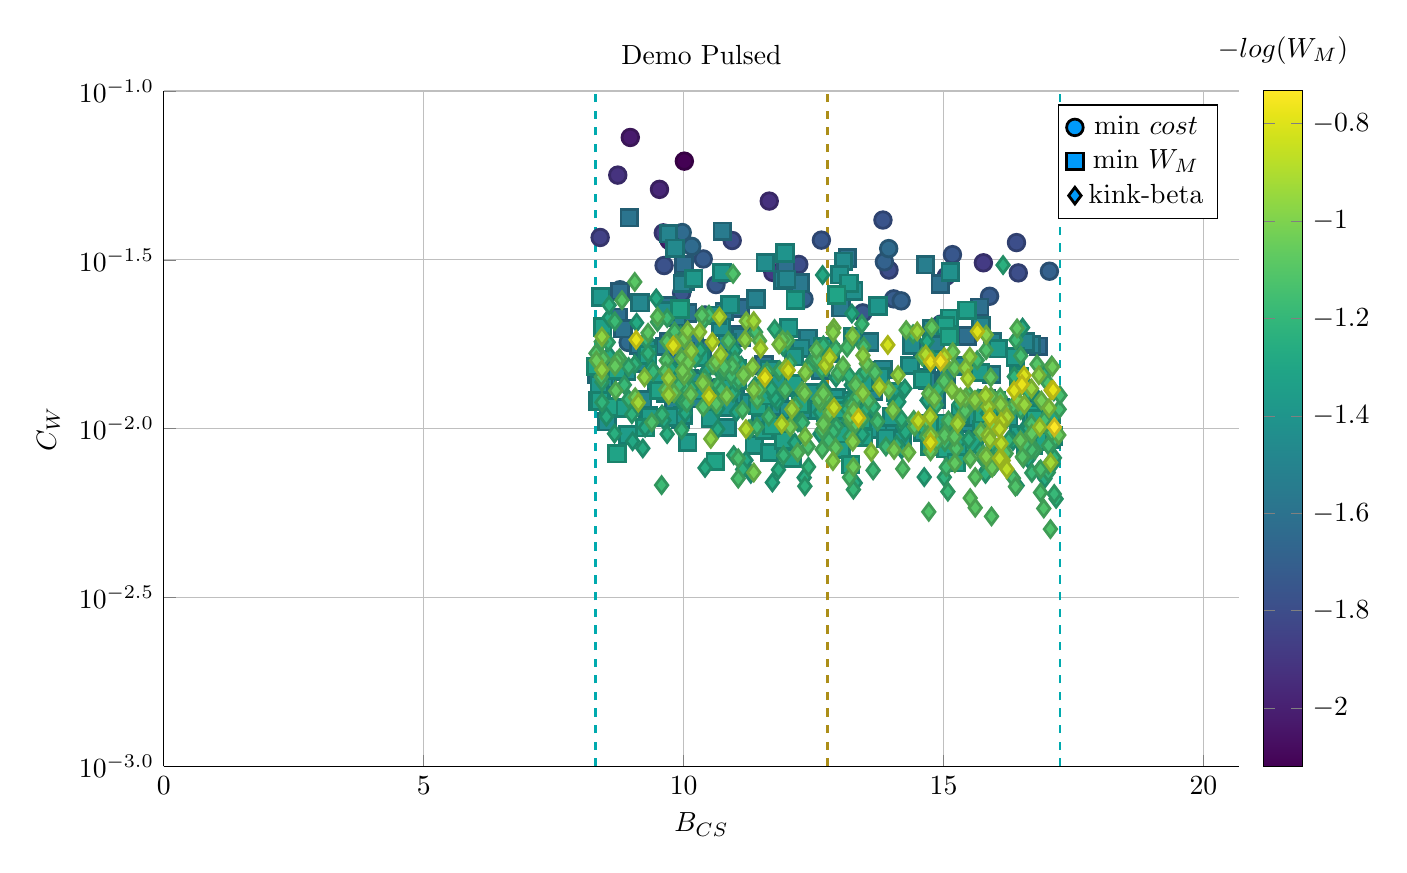
\begin{tikzpicture}[]
\begin{axis}[colorbar = {true}, height = {101.6mm}, ylabel = {${C}_{W}$}, title = {Demo Pulsed}, xmin = {0.0}, xmax = {20.686629468551892}, ymax = {0.1}, ymode = {log}, xlabel = {${B}_{CS}$}, {unbounded coords=jump, scaled x ticks = false, xticklabel style={rotate = 0}, xmajorgrids = true, xtick = {0.0,5.0,10.0,15.0,20.0}, xticklabels = {0,5,10,15,20}, xtick align = inside, axis lines* = left, scaled y ticks = false, yticklabel style={rotate = 0}, log basis y=10, ymajorgrids = true, ytick = {0.001,0.0031622776601683794,0.01,0.03162277660168379,0.1}, yticklabels = {$10^{-3.0}$,$10^{-2.5}$,$10^{-2.0}$,$10^{-1.5}$,$10^{-1.0}$}, ytick align = inside, axis lines* = left,     xshift = 0.0mm,
    yshift = 0.0mm,
    axis background/.style={fill={rgb,1:red,1.00000000;green,1.00000000;blue,1.00000000}}
, colormap={plots}{rgb=(0.26700400,0.00487400,0.32941500), rgb=(0.27794100,0.05632400,0.38119100), rgb=(0.28291000,0.10539300,0.42690200), rgb=(0.28229000,0.14591200,0.46151000), rgb=(0.27619400,0.19007400,0.49300100), rgb=(0.26514500,0.23295600,0.51659900), rgb=(0.25042500,0.27429000,0.53310300), rgb=(0.23360300,0.31382800,0.54391400), rgb=(0.21813000,0.34743200,0.55003800), rgb=(0.20123900,0.38367000,0.55429400), rgb=(0.18555600,0.41857000,0.55675300), rgb=(0.17117600,0.45253000,0.55796500), rgb=(0.15772900,0.48593200,0.55801300), rgb=(0.14618000,0.51541300,0.55682300), rgb=(0.13374300,0.54853500,0.55354100), rgb=(0.12346300,0.58168700,0.54744500), rgb=(0.11948300,0.61481700,0.53769200), rgb=(0.12632600,0.64410700,0.52531100), rgb=(0.15014800,0.67663100,0.50658900), rgb=(0.19109000,0.70836600,0.48228400), rgb=(0.24607000,0.73891000,0.45202400), rgb=(0.31192500,0.76782200,0.41558600), rgb=(0.37777900,0.79178100,0.37793900), rgb=(0.45867400,0.81636300,0.32972700), rgb=(0.54552400,0.83803900,0.27562600), rgb=(0.63690200,0.85654200,0.21662000), rgb=(0.73088900,0.87191600,0.15602900), rgb=(0.81457600,0.88339300,0.11034700), rgb=(0.90631100,0.89485500,0.09812500), rgb=(0.99324800,0.90615700,0.14393600)}, colorbar style={title=$-log( W_M )$}}, ymin = {0.001}, width = {152.4mm}]\addplot+[scatter, scatter src=explicit, only marks = {true}, color = {rgb,1:red,0.00000000;green,0.60560316;blue,0.97868012},
draw opacity=1,
line width=0,
solid,mark = *,
mark size = 3.0,
mark options = {
    color = {rgb,1:red,0.00000000;green,0.00000000;blue,0.00000000}, draw opacity = 1.0,
    fill = {rgb,1:red,0.00000000;green,0.60560316;blue,0.97868012}, fill opacity = 1,
    line width = 1,
    rotate = 0,
    solid
}] coordinates {
(10.014310061470209, 0.06197483174638786) [-2.119809409407475]
(8.974351824202143, 0.07282952610606806) [-2.022107373269494]
(9.720840649522977, 0.03609135913093006) [-1.9777667149411715]
(9.535747921961464, 0.051130362720294704) [-1.969913275543008]
(11.64719575750508, 0.047199699242522014) [-1.9276279243167613]
(8.733488072843636, 0.05634035623848662) [-1.9180907603558137]
(11.717151268119157, 0.0290156978870517) [-1.8866814459155106]
(15.76615725864231, 0.030992141550921816) [-1.8810042714594786]
(9.609717770109604, 0.03801538835634297) [-1.861231108978198]
(8.394527886005427, 0.03683114347875789) [-1.8558362580925096]
(15.053294230728687, 0.028291519575269056) [-1.811508198071671]
(10.934532396569558, 0.03607745072820276) [-1.8048956433290855]
(12.215380678409446, 0.030644555029908985) [-1.797922304180305]
(13.950900000393457, 0.02949537628440487) [-1.7974494679074275]
(16.437201647022366, 0.028933124859920306) [-1.7961193741663348]
(16.40261361811642, 0.03557653455378664) [-1.7922955251500743]
(9.624471357573801, 0.030417392770278703) [-1.7763653379983415]
(13.834221351663881, 0.04147970255534964) [-1.762574168304495]
(9.962006621581514, 0.025210912703269035) [-1.7524000959584443]
(12.65031002841598, 0.036173737778618126) [-1.7467043012053995]
(15.171180859324355, 0.032766263996239824) [-1.7445197156480476]
(13.447185867051214, 0.02202338694073385) [-1.7362913649987812]
(10.622905984575329, 0.026714074548194577) [-1.7340594740544224]
(9.687508349386887, 0.022713661122324157) [-1.7289223235866222]
(15.885358349462447, 0.02466928657304406) [-1.719614121069955]
(14.041145822343132, 0.024233508820652228) [-1.7167136137505041]
(10.377907964259716, 0.03181143352229567) [-1.7154437116459917]
(10.753780577931199, 0.028622291298276443) [-1.7060722509483957]
(17.03614113083419, 0.02926238447048653) [-1.6937830944780397]
(13.861622812084057, 0.03120868171359675) [-1.6889812321302553]
(14.184282250063832, 0.023905595143656186) [-1.686209077026567]
(12.315442430684204, 0.024204963735087338) [-1.6786883535604935]
(14.950434999553853, 0.020413682949498045) [-1.6734478593396724]
(10.4122328117203, 0.02171708878277083) [-1.650681965327452]
(8.776130848827346, 0.025789595420542006) [-1.6458495153344535]
(13.944616671700327, 0.034141771708853026) [-1.6412636709027566]
(9.972964073735131, 0.03809649700399676) [-1.6393314314904326]
(10.155668028711606, 0.0346599142742729) [-1.6390302509540549]
(8.93332912842768, 0.018002375584230325) [-1.6381696948341165]
};
\addlegendentry{min $cost$}
\addlegendentry{min $W_M$}
\addlegendentry{kink-beta}
\addplot+[scatter, scatter src=explicit, only marks = {true}, color = {rgb,1:red,0.00000000;green,0.60560316;blue,0.97868012},
draw opacity=1,
line width=0,
solid,mark = square*,
mark size = 3.0,
mark options = {
    color = {rgb,1:red,0.00000000;green,0.00000000;blue,0.00000000}, draw opacity = 1.0,
    fill = {rgb,1:red,0.00000000;green,0.60560316;blue,0.97868012}, fill opacity = 1,
    line width = 1,
    rotate = 0,
    solid
}] coordinates {
(16.82228492576424, 0.017540808339758972) [-1.6348798048481208]
(11.091923619988552, 0.022785258097976623) [-1.6277277898588538]
(10.00476818341642, 0.030625514244526048) [-1.627684330571819]
(8.777176250808912, 0.025489957683783454) [-1.6248467182009472]
(10.991846079958428, 0.0189830433690413) [-1.62256122166559]
(15.458683088869776, 0.018838350678554387) [-1.6197529434592726]
(11.964070298839442, 0.030553347689269015) [-1.619473374550493]
(8.73450389120548, 0.0213568595963161) [-1.6190205769362032]
(14.592694375647465, 0.017173711360022336) [-1.617478678707941]
(15.693294727899161, 0.022891816741403965) [-1.6135161817566324]
(14.936949374526826, 0.026834336105762403) [-1.6079101518459553]
(8.83184401567771, 0.01976733422078956) [-1.6005797137016178]
(9.72150547040655, 0.01811055755791537) [-1.5991182248913247]
(10.078203743630864, 0.02202289176749285) [-1.595836360479248]
(8.954209756242996, 0.042161103004000076) [-1.589397412964098]
(9.673607099925281, 0.0231728109038665) [-1.589205111302375]
(11.543935756448146, 0.015450272567257462) [-1.5875377953010883]
(13.151617966814817, 0.0319953061173649) [-1.5845809864087244]
(9.781030534247606, 0.016164039710660088) [-1.5775674018565111]
(9.303102469493684, 0.016693759971981265) [-1.5713155071601692]
(10.359872502096119, 0.01726409176752251) [-1.5652457853616617]
(12.237632180874417, 0.02698353416604086) [-1.5643952661253622]
(9.144801617136775, 0.01769761001811183) [-1.5595601870169422]
(13.029635600163276, 0.02281153437267921) [-1.552568848396255]
(10.7422001331706, 0.038423068705951594) [-1.5520441226990631]
(10.780757247562724, 0.022224095489930037) [-1.544925041354305]
(10.200715682654506, 0.01841847429182733) [-1.5430023738862098]
(15.017329028039686, 0.019477644457703495) [-1.5396243114452017]
(8.334002624663501, 0.01449908817629988) [-1.538692217528126]
(10.555701885198872, 0.013092644307368572) [-1.5373740781698282]
(14.65414605441725, 0.030574977212997605) [-1.5350312948909135]
(14.660222353908768, 0.014205258889817484) [-1.5317433014682034]
(11.106568774256633, 0.018689708848548738) [-1.5311850486265117]
(14.689056206740792, 0.01387590038164943) [-1.5287451237254033]
(9.473959265162193, 0.013905952265261586) [-1.526526816139614]
(10.035372496295135, 0.027241135712482305) [-1.519178921439465]
(10.039027121575653, 0.016910779414334946) [-1.517891032933806]
(11.39227618908412, 0.024191852864153648) [-1.5130165343032327]
(16.679321236285688, 0.01773125993862434) [-1.5126055054907948]
(11.906042879430306, 0.027530426264504002) [-1.5122759735909235]
(13.642157714321597, 0.014899481481132758) [-1.5121531835443067]
(14.850116736119897, 0.01778122202031051) [-1.5121518481580156]
(12.392450828732116, 0.01852162588841651) [-1.509963665969106]
(11.613487062213123, 0.013259386458548635) [-1.5098191352881933]
(13.579000388347866, 0.018078145365757758) [-1.5094600237705913]
(9.867201865947047, 0.02134336001409843) [-1.5091677016781566]
(9.643385161260726, 0.017507453096671365) [-1.505813383704145]
(9.97586799244543, 0.026909424888676328) [-1.5035180904231982]
(15.94212072748298, 0.018116695499993292) [-1.4998070828001184]
(10.309179324950696, 0.01226652304303364) [-1.4993412700061268]
(12.638042249859588, 0.014898889997617197) [-1.4970388348465338]
(15.055675671525783, 0.014279317114283529) [-1.4968151314329754]
(9.710222870228767, 0.03778412752723575) [-1.4959262215207656]
(9.813107231605422, 0.012007443130458324) [-1.495878750102406]
(9.685925965003944, 0.014131383104205364) [-1.4911760171512294]
(11.714098265194735, 0.013847785437885679) [-1.4909012021072667]
(10.994639674638705, 0.013113327535403696) [-1.4904727997922445]
(15.819989093254375, 0.012253217681920671) [-1.4902975254497872]
(15.716610680795545, 0.020179920200301855) [-1.4899596862430686]
(15.924465247564154, 0.014465480638895564) [-1.484315053758591]
(8.416214966248592, 0.012974868808400592) [-1.4832272441818983]
(11.981607928881237, 0.02767164571202513) [-1.481908947186888]
(11.711067257135763, 0.012700241486954703) [-1.481610811848838]
(16.57758432667383, 0.018066556725317685) [-1.4808315890609627]
(9.214130290028436, 0.012152582495637852) [-1.4803924190961808]
(9.16252648162826, 0.023591043628319753) [-1.4777813991456452]
(13.841485576616298, 0.014987126189756067) [-1.476226145125234]
(14.86036210936636, 0.012179602718049342) [-1.476103765156545]
(14.771702357628312, 0.0198044997246676) [-1.4759532635696884]
(11.751019990155784, 0.011854698849849837) [-1.4744693843941874]
(9.214130290028436, 0.015665176708494814) [-1.4721189566530006]
(13.644386027863185, 0.012892988065699775) [-1.4694765884704042]
(12.673551051198132, 0.011723605612914264) [-1.4684762544315009]
(16.7437460203336, 0.01146148363735155) [-1.4673712598422484]
(10.114476569413018, 0.01403086783418577) [-1.4665127712450712]
(9.836829838606402, 0.03422172209265897) [-1.466465342676487]
(15.478205114940627, 0.011814056076879775) [-1.4656409913573911]
(10.852786830516008, 0.01666169164744686) [-1.4607639902508311]
(12.451557765219139, 0.011797068547740396) [-1.454804800167485]
(14.385054216404878, 0.017714850999176746) [-1.454016548396377]
(12.250517419581046, 0.01730924236440855) [-1.449126660054787]
(15.399238782030915, 0.015350811156516968) [-1.4450317564339483]
(15.323964495196108, 0.010700521525178483) [-1.4442476160174416]
(10.840350242413816, 0.017999193081243068) [-1.4428695943470562]
(13.07657469813823, 0.03129913412451443) [-1.4416527786165851]
(11.571153759168391, 0.030992801350489627) [-1.4412978501823663]
(10.159175807081688, 0.013876797144792313) [-1.4410674847520173]
(14.65870048492913, 0.0103371343106061) [-1.4407593364531412]
(9.64911680597678, 0.022291694526716137) [-1.4382523340904476]
(11.824660750219888, 0.011033535668865918) [-1.4374618391296154]
(16.090603216081107, 0.011578760205733224) [-1.437309497392895]
(8.526794202732354, 0.014225493350487712) [-1.437004502630189]
(11.836002040544534, 0.011662685993065088) [-1.4369516286418977]
(15.4684670810238, 0.010363517857158673) [-1.4359296968945898]
(11.551257449345478, 0.012593943496598788) [-1.4348111698815942]
(8.523380131000312, 0.010486068251726523) [-1.4347403934029699]
(12.329900028804074, 0.011351647420548932) [-1.432162507533083]
(13.236600826453692, 0.010703895251080882) [-1.4298959659652046]
(16.83282359352303, 0.010279170294604838) [-1.429141349371285]
(13.269307990860742, 0.025557043779995653) [-1.4288294492620477]
(10.717109038917776, 0.019981046165081038) [-1.4275892047251812]
(8.463326863230373, 0.014011150106021747) [-1.42664672926539]
(9.292495803166666, 0.017276630179413652) [-1.4239039330716527]
(12.01294221545527, 0.01135063897630595) [-1.4237047673472223]
(10.642574031409726, 0.021651736693319764) [-1.4220880228019461]
(15.130371291452986, 0.029124606257697153) [-1.4214589216983458]
(13.449121379363364, 0.010524080735331771) [-1.4192750546166355]
(10.598536227766495, 0.012152497168515361) [-1.4188846212567885]
(9.94286005160173, 0.010654264771940928) [-1.418142111238707]
(8.354283940274188, 0.012093014306414056) [-1.4175771687309422]
(11.490654672775422, 0.010307835186267926) [-1.4166515403180218]
(13.927755889931667, 0.009802839106844477) [-1.4151591623618127]
(12.896498202515414, 0.012089411129630757) [-1.415086999740124]
(12.813665090982388, 0.016771907819218872) [-1.4150518254702726]
(8.905845640255238, 0.01479570625667246) [-1.412750376425469]
(13.001742838316293, 0.02858609969916251) [-1.4118418857799215]
(14.802174067631956, 0.009976658176736495) [-1.411745253778192]
(11.208912070421409, 0.011899859669740264) [-1.4101129990450592]
(12.913000276070724, 0.010975696046095008) [-1.4098064292280077]
(10.84161307277213, 0.010078193568331789) [-1.4071217370506766]
(10.952245284131447, 0.012567870805096065) [-1.4069653518342513]
(15.465550241086678, 0.010809590548122633) [-1.4053188021751997]
(11.888760566686239, 0.013228123351848638) [-1.4040831795581317]
(9.656977955682123, 0.012756284815624411) [-1.403783408224447]
(12.357969070297273, 0.011849909135487101) [-1.4034059706684434]
(14.354705949019486, 0.015391572104901911) [-1.4031334212883295]
(15.759091197715701, 0.011370525417095621) [-1.4027031557706915]
(15.93492167661274, 0.010883116023126084) [-1.4023409214316394]
(11.950351989604266, 0.03314304390232683) [-1.4018234466267534]
(9.31395933016945, 0.010943279854872806) [-1.4001967788421508]
(12.501198744996175, 0.012776602146795163) [-1.3983213447403338]
(16.691702745627914, 0.011065372696240975) [-1.3946316971345938]
(12.793680134727829, 0.009697674748088487) [-1.393981306323598]
(12.945145532203291, 0.012316212001497684) [-1.3939743444895971]
(10.895241072523511, 0.023293627402023516) [-1.3938659098694006]
(10.624418674781085, 0.012799262525216688) [-1.3934317035795]
(13.736998867652822, 0.02306752096780418) [-1.3919378361313393]
(10.86446674023058, 0.011575943181240602) [-1.3913501343623875]
(9.989604552735361, 0.010938935413839007) [-1.3899986150261634]
(11.65036209258509, 0.014916276865219583) [-1.3888953225499234]
(16.253794354777128, 0.010811642128190005) [-1.3883849558567678]
(13.237511348589962, 0.012086573842968483) [-1.3880683151937296]
(13.3098445206835, 0.00974951527611275) [-1.3879257169733152]
(13.250391582535599, 0.01875474559032549) [-1.387200255154835]
(10.737511566041665, 0.028992717747430105) [-1.3869139374162498]
(13.77662330230216, 0.014275341697562267) [-1.385982080919773]
(15.808216920395289, 0.009658736241223327) [-1.385951966541943]
(13.731078012406766, 0.009979205376142167) [-1.384341496966052]
(14.597629824496682, 0.009781750047901397) [-1.3836628266676982]
(10.193517952021443, 0.027837899406166513) [-1.383138617240496]
(11.85882016006122, 0.013692957043690078) [-1.3831333668949872]
(15.990533435344123, 0.012055028195149642) [-1.3823755173012382]
(8.403151177328072, 0.02457168150365556) [-1.381386436684111]
(8.38045546510813, 0.013467436970042478) [-1.381013926041926]
(12.120810510968868, 0.01632900764605371) [-1.3807582017142732]
(10.203415923531363, 0.016233342907168043) [-1.3795912650626003]
(12.022820996636117, 0.019856726760879642) [-1.3784744825946547]
(14.941654987190931, 0.009937020814786353) [-1.3784050115817357]
(10.30431640058217, 0.012947457233964572) [-1.3727350903904059]
(13.179314023604123, 0.02692798924274793) [-1.3726382795387042]
(11.360939883051167, 0.00894061047284123) [-1.3726183217257064]
(9.712824116971364, 0.01083618948017438) [-1.370506635821487]
(13.999353699862713, 0.010820381028973857) [-1.3702834841058706]
(11.029519708444795, 0.01507474130083674) [-1.3699905172740252]
(14.790388677939154, 0.016024901755414496) [-1.3694510931398833]
(14.2011289491935, 0.009286958803152093) [-1.3690194932725448]
(16.05186059099198, 0.01725165686414962) [-1.3685993689556193]
(10.079551280694128, 0.009100422809121853) [-1.3680782620249432]
(13.891099279827657, 0.009358898748733285) [-1.3659937757563743]
(10.51469839684549, 0.010741593794976297) [-1.3655266043175585]
(16.97679926285361, 0.00935804014953258) [-1.365489135635999]
(16.382025622806193, 0.01631624677926724) [-1.365314944668722]
(12.601871821561915, 0.011316654652064283) [-1.3620488306806053]
(9.342717740515683, 0.010811158792461435) [-1.3600883836878876]
(15.699013106793902, 0.014663988794896813) [-1.3569999482959285]
(17.08124053314885, 0.009327975573933072) [-1.3565369493574833]
(8.929819918270683, 0.009591330831744169) [-1.3564434514013937]
(17.107810871536294, 0.009510520762087537) [-1.355670949654743]
(15.272532347809275, 0.008600603815848054) [-1.3550689180362785]
(15.113272758939148, 0.0212306523206366) [-1.3545717493575382]
(12.758115395547385, 0.011027495783414606) [-1.3536406793714741]
(12.146510141523258, 0.02403578580290836) [-1.3522480304376618]
(9.802895887224908, 0.01277987363566607) [-1.351683168790268]
(12.731812711004267, 0.011181317227288103) [-1.3509416538039447]
(14.597629824496682, 0.013988110662625983) [-1.350917699634303]
(12.937418062164188, 0.011706003302806382) [-1.3498675794038522]
(12.680634700802198, 0.01744787935363008) [-1.3480954361555229]
(16.547895069902516, 0.009513333911267541) [-1.3474307155472665]
(11.653216567545261, 0.008506399274340092) [-1.345835600508895]
(15.44880839508013, 0.022402494346273383) [-1.3441619287129023]
(11.525312140201327, 0.011568935524735228) [-1.343173024895477]
(11.552250427675727, 0.009888039453025594) [-1.3431102335422052]
(13.467268933575436, 0.013676025720795522) [-1.3418959513921676]
(15.323265928492141, 0.011055478792069253) [-1.3416390955818198]
(12.121641590617898, 0.013562184857025608) [-1.3412225668983788]
(11.024065356801717, 0.013928329166195007) [-1.3411223781363122]
(16.734724817567656, 0.008957609956171385) [-1.3409980727589041]
(16.769045540215842, 0.011061155580644737) [-1.3407774046291352]
(9.473959265162193, 0.014142372730384274) [-1.340736718067575]
(8.74505555084563, 0.014931289500105476) [-1.340172101894623]
(13.027598279499255, 0.008673821452175847) [-1.339371225527388]
(14.069726621490684, 0.012851757813003692) [-1.3355889626958743]
(16.45157670371507, 0.009585198585080813) [-1.3353537500446666]
(8.828372531773972, 0.011502571386254939) [-1.3352936153265889]
(15.043191855376238, 0.020177908654106694) [-1.3347167954999664]
(15.87555423129121, 0.010934192827515073) [-1.3333464153994234]
(14.74050555979749, 0.010187040046408826) [-1.3319467069356516]
(8.394635001603197, 0.012093243108414115) [-1.3317606682979195]
(15.737459460817936, 0.0099544891977854) [-1.330878268232421]
(16.577004376563345, 0.00892167491417854) [-1.329838199225075]
(8.442119987401155, 0.020024514359414238) [-1.3275817805394716]
(15.03780769292473, 0.010377685225384297) [-1.3271981479523673]
(11.923687420170552, 0.00923521460571462) [-1.3257753666633474]
(9.311244990438865, 0.016536435428404248) [-1.324805801675252]
(12.08205721926947, 0.008177838551829547) [-1.3236480395933032]
(10.75205842676705, 0.01320289357034274) [-1.3223872875360454]
(13.461717625918478, 0.009416665871049234) [-1.320790714548859]
(9.519960674752117, 0.012966997564871513) [-1.3198610091294973]
(8.715815013641683, 0.014941915896507264) [-1.3173999901029887]
(9.815532890733682, 0.014705731648914599) [-1.3172398911361078]
(15.109422453252336, 0.018745840734049092) [-1.3155841266914403]
(14.740296253242736, 0.008883845818604448) [-1.3144429555765318]
(10.31653236444549, 0.016334708642476756) [-1.3140984246311314]
(10.60954534582113, 0.007999169369094802) [-1.3136141988883636]
(13.432319600929263, 0.010593671042148305) [-1.3130409307938926]
(11.42823386655995, 0.011696426000066894) [-1.312883593567563]
(8.719380611168567, 0.008437215022084032) [-1.3113636666391015]
(11.696923395666094, 0.010210442889078589) [-1.3110543205827916]
(8.560854879579562, 0.01161135507437133) [-1.3101666476591896]
(16.764368284085073, 0.010715857251244127) [-1.3094281744638252]
(15.192999611497397, 0.007935513211517508) [-1.3092819198295769]
(8.315725665672304, 0.01527961135499392) [-1.3091789421820008]
(15.043366759433116, 0.008718673720708605) [-1.308657609117127]
(16.021238035205084, 0.012115862676003172) [-1.30815684782275]
(11.593073557294613, 0.012528702800938256) [-1.3073192126014976]
(15.192999611497397, 0.009466859805614364) [-1.306104667504652]
(12.945145532203291, 0.024862203238592617) [-1.3061029424340123]
(9.927382980222017, 0.022588731344076834) [-1.3059932173472433]
(9.256949266351661, 0.010067194372351543) [-1.3053424100316993]
(16.82199006964077, 0.009194414774426339) [-1.3048906180553326]
(16.45157670371507, 0.014224364223609164) [-1.3043596581137094]
(13.051048964875424, 0.00966642720928779) [-1.304157201921016]
(15.244913096432274, 0.007934056288357859) [-1.3040523349428945]
(12.245141259071001, 0.011830250137913223) [-1.3039439069452712]
(16.026769470614276, 0.008152912507864905) [-1.3022467953572583]
(13.051048964875424, 0.011323662495891916) [-1.3012176243848619]
(15.591542980066137, 0.009074217857747638) [-1.3011866801418175]
(17.068912884842916, 0.011011974496683653) [-1.3004916659282275]
(13.212953491584514, 0.007824745570931163) [-1.3001880033121107]
(15.749170807222828, 0.011078402389842862) [-1.2993649239636758]
};
\addlegendentry{min $cost$}
\addlegendentry{min $W_M$}
\addlegendentry{kink-beta}
\addplot+[scatter, scatter src=explicit, only marks = {true}, color = {rgb,1:red,0.00000000;green,0.60560316;blue,0.97868012},
draw opacity=1,
line width=0,
solid,mark = diamond*,
mark size = 3.0,
mark options = {
    color = {rgb,1:red,0.00000000;green,0.00000000;blue,0.00000000}, draw opacity = 1.0,
    fill = {rgb,1:red,0.00000000;green,0.60560316;blue,0.97868012}, fill opacity = 1,
    line width = 1,
    rotate = 0,
    solid
}] coordinates {
(14.682772921069034, 0.012133883145293747) [-1.2971735267311564]
(16.555137236197424, 0.008497507185750146) [-1.2963451470925318]
(13.179991464330723, 0.011968595839803002) [-1.2939289874566402]
(15.888696111510232, 0.008051203599652048) [-1.2928570974581939]
(16.651463466334494, 0.009198462479520332) [-1.2926592596370523]
(16.555137236197424, 0.009976448637174172) [-1.2918359622137705]
(11.015371517921224, 0.011200517330116096) [-1.2901565279273088]
(10.43448368514836, 0.014778677283745992) [-1.2885231243501492]
(12.62262254375668, 0.009645840422057206) [-1.2873870680148987]
(11.10781988195937, 0.015368153744705897) [-1.2867189599495152]
(16.82199006964077, 0.012200186404574626) [-1.2866608738447551]
(15.327000264646497, 0.009314200607444962) [-1.2862989627940875]
(11.293041040527157, 0.007351086075188858) [-1.2856479743658245]
(12.62262254375668, 0.011184811263709776) [-1.283461572944208]
(12.673551051198132, 0.028511756618296732) [-1.282628142229196]
(9.018740260054527, 0.0091809969411667) [-1.282318795548118]
(9.378254722237372, 0.015147418693115068) [-1.2809419797501462]
(16.67207354194001, 0.009441743395354373) [-1.2802239523296417]
(14.221898977802105, 0.010115067051441084) [-1.279661807174519]
(14.193898850417899, 0.008682653521467484) [-1.2793586996677089]
(16.335988065907316, 0.00919694313697991) [-1.279241431080542]
(11.199032883922865, 0.008062649665833432) [-1.2791738597664242]
(8.565625511562189, 0.016537125137685977) [-1.2777724695025643]
(9.473959265162193, 0.024311609583825906) [-1.2776560252665474]
(15.820537682670786, 0.007543708329813699) [-1.2776226586446298]
(13.223938971427943, 0.013472425466080754) [-1.2772080908839465]
(9.6224419440208, 0.010591022499429533) [-1.2768888641183538]
(9.259381405997736, 0.010068814155906535) [-1.2749252706301877]
(10.02950074316046, 0.011122028940902477) [-1.27405635520294]
(9.096410727756737, 0.020592443763116842) [-1.273999627133777]
(11.250274296159523, 0.009932693135460512) [-1.2739263340884897]
(16.651463466334494, 0.013177764718534145) [-1.273686836355838]
(13.236600826453692, 0.021930543698997433) [-1.272060671091855]
(10.988390518242154, 0.01703366147805158) [-1.2717552020206426]
(12.689774417510133, 0.013199694993892157) [-1.2715552113887816]
(14.682772921069034, 0.018137179053328113) [-1.2711256143593725]
(12.138235311074201, 0.009089213335736035) [-1.2706918059143955]
(16.51983071545539, 0.019922160606497104) [-1.270659241243097]
(13.440224729488612, 0.009612072783370788) [-1.2706266042708976]
(14.056438663449487, 0.011815687417752718) [-1.2699973230973551]
(16.632293213183402, 0.008127375094877596) [-1.2694883213650459]
(15.843105813982604, 0.011108460101523684) [-1.269469949244091]
(14.139022745673238, 0.01200413289507089) [-1.2693810054133523]
(8.565625511562189, 0.021322131632939743) [-1.2685038799823198]
(9.215460716271485, 0.008746022086925008) [-1.268011220133286]
(11.79925508433291, 0.012071261699451271) [-1.2676767161765092]
(9.767648689516832, 0.015027760071695463) [-1.2672360183442966]
(9.905927226247794, 0.012386782250268949) [-1.2670329245716005]
(10.65725161660864, 0.00997135774995843) [-1.266521603924258]
(10.055681915858392, 0.014743359804979298) [-1.265829536383991]
(12.138235311074201, 0.011015221663609409) [-1.2655850749955841]
(14.267102900143742, 0.009754591610171831) [-1.2651606387913807]
(16.568716501758974, 0.008391084675782472) [-1.2650267302153226]
(10.65725161660864, 0.011459660264397842) [-1.2643165163116283]
(14.25689481086506, 0.01314380020899071) [-1.2638630587832318]
(16.632293213183402, 0.0100188505842072) [-1.263682663264664]
(11.707584495779955, 0.006930908540990179) [-1.2635507051033026]
(10.412391370371594, 0.007655768190498255) [-1.2630930817893484]
(15.707955638238712, 0.008595102325139414) [-1.2620028969039807]
(15.941689167985352, 0.008993269936185943) [-1.2617711256664215]
(11.618449420251658, 0.013435175267701598) [-1.2607622270815175]
(11.906052951232901, 0.010399130132164968) [-1.2599969566754825]
(13.422765787398976, 0.011066872440514844) [-1.2580199333772297]
(12.931935336308614, 0.014164623239439114) [-1.257674742909116]
(16.4155019400067, 0.006784814729690784) [-1.256920205986828]
(8.514832197721942, 0.010847484174753686) [-1.2558826127376497]
(9.960307841751561, 0.012006910499828622) [-1.2545784323742915]
(11.751019990155784, 0.012367303307791636) [-1.2541769145790829]
(13.300908706718086, 0.006909773766752695) [-1.2538081670568602]
(16.949195577210475, 0.007118806510545466) [-1.2537331036632384]
(12.318542112721676, 0.007163920014099904) [-1.2523947287534352]
(9.960307841751561, 0.01409766195530951) [-1.252161894882265]
(14.628561786858135, 0.007191926525759095) [-1.2517841257242934]
(15.90674460516089, 0.010140660180167243) [-1.2510148685101052]
(12.87923916901645, 0.009947685467565285) [-1.2503817284236358]
(11.824591933033416, 0.00755783116205777) [-1.2500618007814928]
(10.31927503264005, 0.01705584468677382) [-1.249408930050928]
(15.977434181824485, 0.007782048369656626) [-1.248434923528094]
(9.683456615169344, 0.009638865392082259) [-1.246475793101881]
(8.671623187801623, 0.009668090359024908) [-1.2453083223674235]
(15.299311115315916, 0.01181801423349667) [-1.2430271033455136]
(10.952245284131447, 0.012765537294567253) [-1.2425009663963265]
(13.37865937666007, 0.014096920088512531) [-1.2420036959161107]
(11.040941770182885, 0.014638041989732616) [-1.2406291651922927]
(13.488578301097156, 0.011330221246013529) [-1.2404081246835275]
(14.628561786858135, 0.009882346466549934) [-1.2402721066912186]
(16.145232878087864, 0.030517882462548936) [-1.2399829928026451]
(9.943887569980818, 0.018855374361929193) [-1.2398403601837327]
(11.689159647203805, 0.013105067185166342) [-1.2382227382575577]
(8.567148568313412, 0.023206171452307512) [-1.2372685823332665]
(11.915585134033648, 0.01748239328622686) [-1.2369979991721363]
(12.198645212509877, 0.010436966421480154) [-1.2364971528125899]
(15.48431465614079, 0.00929031971105747) [-1.235918342000411]
(9.047649397424134, 0.01224311754662533) [-1.235332112263366]
(11.376707871371156, 0.013377000135851953) [-1.235230354209212]
(16.840748740961537, 0.00752176857171885) [-1.2348662947331168]
(11.136175174634447, 0.007577390318458053) [-1.2331237451825037]
(14.097655097755435, 0.008954934736687754) [-1.2314216648450123]
(15.807042377277515, 0.007348723496235854) [-1.2276908244938955]
(12.33207356829479, 0.00675688814735783) [-1.2234874983546444]
(10.222252038737434, 0.01611655322423877) [-1.2224132121245386]
(16.251358747135995, 0.009234491873309686) [-1.2212129344183997]
(12.723834447815875, 0.012691970303684906) [-1.221000044288545]
(9.004625505986517, 0.011032294768272291) [-1.2201668573985105]
(10.678976402706837, 0.014875616723151944) [-1.2200113852982524]
(13.05961095465478, 0.014755597501979523) [-1.2200110437170943]
(9.058040813922531, 0.015480160187022769) [-1.2199386530853975]
(11.751019990155784, 0.019725018407248666) [-1.2192027637421239]
(15.662199761760458, 0.01227428321856098) [-1.218844626416703]
(11.002753780917594, 0.013727476887235461) [-1.2187513907488479]
(15.014532020154196, 0.007184219051293641) [-1.2182120816961266]
(13.148749979709805, 0.011425165896800414) [-1.2178523450390264]
(9.316969297353253, 0.01671459075301228) [-1.217564445140848]
(10.154270603961049, 0.01316079396243774) [-1.2148287908302686]
(14.19279870188835, 0.010653867811546877) [-1.2144650329368094]
(17.165092473837838, 0.006198307301760009) [-1.2142295699793069]
(15.014532020154196, 0.009725241928162248) [-1.2114971471794018]
(10.964602796324286, 0.00834877000609595) [-1.2110590840755884]
(12.25459113238908, 0.010394495894857034) [-1.210956786812969]
(13.649393629962841, 0.01160689504064373) [-1.210625479626572]
(12.40274647042282, 0.007709496307162327) [-1.210548450407708]
(8.42941267292461, 0.01196700634860152) [-1.2101072964851303]
(16.360665913232772, 0.014267222031421351) [-1.2097043828037173]
(12.688686022519612, 0.017649120721508472) [-1.2090548152300868]
(17.101933862003563, 0.00786922573538261) [-1.2089432452477198]
(13.212953491584514, 0.018050177035811292) [-1.2088567702310062]
(8.42941267292461, 0.01374396978202603) [-1.208355792529063]
(15.807042377277515, 0.012119563498851512) [-1.2079597098695036]
(11.826932290539112, 0.01476620759208673) [-1.2069143247822283]
(16.937250320827843, 0.014425121215984256) [-1.2060355587049236]
(16.56929514507332, 0.008818373193963157) [-1.2051439881244612]
(13.181524156722897, 0.014347196234709005) [-1.2048202874468241]
(14.89986738586979, 0.013090961135950088) [-1.20412102013171]
(17.131922906542755, 0.008195788944222735) [-1.2006084749599055]
(9.584782689444218, 0.011017845567179161) [-1.1997509076464346]
(13.490860552242111, 0.01471498897475931) [-1.1989561148134826]
(13.176473234117513, 0.010576750792174504) [-1.1977552093777106]
(10.988245035999599, 0.015955953274896677) [-1.1973464324024234]
(15.038409502255757, 0.014024797653122234) [-1.1952843257986516]
(9.961762717388044, 0.009913142251828634) [-1.194608172565493]
(8.942050925672243, 0.012231614304186931) [-1.1943983553124515]
(17.120985015074893, 0.012895825589119291) [-1.1943709063726027]
(11.920999462954518, 0.008341248647504823) [-1.193465520169887]
(17.014436731421398, 0.007422215660710276) [-1.1934529196767811]
(8.548963250971841, 0.018029259293378272) [-1.1932608414538086]
(9.416726619046099, 0.01475503745943627) [-1.1930245850534404]
(12.4394525554187, 0.01559839957452813) [-1.19275308105931]
(13.265902368751764, 0.006601321305241876) [-1.1925650410586528]
(16.6299411017185, 0.012849471675853265) [-1.1916847830033912]
(17.129202501787184, 0.006406786662781295) [-1.1906829642457115]
(8.942050925672243, 0.015231829402577652) [-1.1905171502567853]
(9.27906715150467, 0.018424630927819426) [-1.1868792227109848]
(10.021428108030735, 0.012087057868798792) [-1.1860893620286155]
(14.77757376918867, 0.016048418150957987) [-1.1858875370196502]
(10.454025691365954, 0.011972397837837176) [-1.1854558952607928]
(8.86037108397972, 0.013483711604703155) [-1.1848213366225184]
(14.860405552114257, 0.011761816070313931) [-1.1847475832442582]
(16.697734081097174, 0.007399398212169979) [-1.1837916630431773]
(12.287202704452202, 0.010413257435217902) [-1.1834175022102877]
(13.199631705820181, 0.009470444499328991) [-1.1831305353511883]
(12.04002156741698, 0.015647472969860403) [-1.1828511911535706]
(13.429268295632518, 0.020407456319850734) [-1.181840770808167]
(15.083042498987238, 0.006510208938595967) [-1.1814651012301538]
(12.93585934283502, 0.010147346100150811) [-1.1809344434678004]
(15.08903520717264, 0.010306295906351105) [-1.1788261142099545]
(12.874280008939282, 0.00975845363999315) [-1.1783873972417303]
(9.683456615169344, 0.021255557406142055) [-1.1773891261145735]
(13.645133488301468, 0.007530050850229014) [-1.1772489110999693]
(13.89170225379231, 0.008856286376022381) [-1.1771937197283155]
(8.67737182027737, 0.02079595788529988) [-1.1768483795316644]
(10.771643002371896, 0.01477464262853022) [-1.1754670828809672]
(10.657856383500425, 0.013447350775475101) [-1.1748259721272571]
(16.06471023259536, 0.008533818365309384) [-1.1743579362801864]
(17.1316836490387, 0.00926629982316415) [-1.1731424023398116]
(15.026041337358697, 0.009127162071787865) [-1.1728411497954707]
(9.576609781620636, 0.006808109484569134) [-1.172547785671985]
(11.279560489781714, 0.009974514104150454) [-1.171293732602548]
(11.847882069406987, 0.014894587057756483) [-1.1706435645347975]
(12.662794223849232, 0.014934801738779929) [-1.1704804143126533]
(16.3897848180077, 0.018312728464608994) [-1.1694340492000508]
(10.730031930410188, 0.013038425730797958) [-1.1664836698360914]
(16.484580953127526, 0.011350876468389677) [-1.166021933665907]
(10.407320998161198, 0.014066615859663486) [-1.1653547583030963]
(11.639069714872814, 0.01085952514652926) [-1.1637013339225117]
(10.006343137186239, 0.013377410828925157) [-1.1629231949973953]
(11.059345377913772, 0.013971916288186385) [-1.1625677338545028]
(12.40274647042282, 0.01498663044146402) [-1.1615160270969884]
(10.06408250853542, 0.011904820041118874) [-1.1613847421954753]
(9.902431073117565, 0.013362365525672213) [-1.161380763910868]
(14.413146086048558, 0.019049310191542535) [-1.1612715538980343]
(11.410705501319088, 0.010122141818818486) [-1.1608808882180581]
(16.090315471306553, 0.011629604231527799) [-1.1602959592128257]
(16.535372216388026, 0.008169777889897055) [-1.1601187846950554]
(16.106899256187383, 0.00834966465898116) [-1.1597072302883453]
(10.09639230576176, 0.014522157751088465) [-1.1596295654776811]
(10.914467071854592, 0.014324434384547807) [-1.1584930595938716]
(15.760042238713773, 0.008145962416336265) [-1.1583013384515075]
(16.758572280032737, 0.008646050418225202) [-1.1578217536561153]
(17.018646604266053, 0.007816314398845932) [-1.1564044749404534]
(12.796253779221516, 0.009241849076330648) [-1.1562110876559482]
(15.052414924338043, 0.007695271029389756) [-1.1558406723410226]
(15.647072980506872, 0.015939165384127457) [-1.1551976368183803]
(13.731078012406766, 0.010505037613581628) [-1.1547723960660046]
(12.92675278881294, 0.01720072822154318) [-1.1547042721803664]
(17.018646604266053, 0.008918107308299703) [-1.1544971334332936]
(16.253794354777128, 0.011156083675037292) [-1.1514583143146417]
(10.39603038372212, 0.021035989307587558) [-1.150606587165903]
(13.463766396551701, 0.017520815218592205) [-1.1497568820513546]
(11.384733765960362, 0.019315926185319167) [-1.1488471764736738]
(16.484580953127526, 0.016442878704583205) [-1.14854127278881]
(11.604112098987112, 0.0147653907680726) [-1.1481443824350337]
(9.497296911957019, 0.02069244645197561) [-1.1475056240535222]
(10.488224449472721, 0.021750535713550727) [-1.147314943378139]
(17.223162892419708, 0.011413531346774588) [-1.1452162507505037]
(12.150894786402327, 0.011657490769208391) [-1.1440985305669964]
(16.68930628775202, 0.008671087589979474) [-1.143892607737901]
(16.569886893433157, 0.008990361186615302) [-1.1425154271844815]
(17.23885789045991, 0.012558201977665608) [-1.1419282223298928]
(16.936340179186345, 0.010576229210216307) [-1.1414111342865825]
(14.737732430469173, 0.010807673225691976) [-1.1409606377195203]
(16.68930628775202, 0.010350872866134037) [-1.140632380055554]
(13.442192340718403, 0.010685556097930418) [-1.1405059694207205]
(16.212323704366778, 0.010680444710790922) [-1.1402761489506106]
(11.549625061051866, 0.01443507208815689) [-1.1390460916159142]
(16.86604828682311, 0.007579718089160525) [-1.1390342976608838]
(17.08124053314885, 0.009743368571375198) [-1.1383859727853913]
(15.465550241086678, 0.011556690979889052) [-1.1378233474839952]
(13.14480493296275, 0.01739508549026366) [-1.1377132966757475]
(13.247068833500391, 0.011726874929476301) [-1.1376503199229564]
(11.050777266016288, 0.007116540390245059) [-1.1370921105287648]
(17.00860271346254, 0.013630883580602493) [-1.136359546149739]
(12.74928812237468, 0.01526251681202216) [-1.1362968805162]
(9.828339372234877, 0.019391120833403556) [-1.1358988321292471]
(16.412079199162257, 0.011860427509089479) [-1.1358539207185072]
(11.050777266016288, 0.008170611753766615) [-1.1356493088623822]
(13.190058867236672, 0.007176648981252689) [-1.1354932328782563]
(16.343118613330425, 0.007134995489417047) [-1.1335001124055868]
(11.133919631731134, 0.011362840629455528) [-1.1323762690185122]
(12.973701334746814, 0.014605309967466338) [-1.1314565774222176]
(11.954226224374837, 0.013041177771875015) [-1.1310401855629826]
(16.86506841916708, 0.006470994712702174) [-1.130758874865596]
(13.342005434244879, 0.01241454353087534) [-1.1307392487451149]
(16.12398815332631, 0.011706749993287805) [-1.129690412643984]
(15.094274129902931, 0.01058602765458819) [-1.1289684185709847]
(12.56748354328549, 0.016110870179123358) [-1.128250192514324]
(13.554151997056962, 0.012109336313631335) [-1.1252475037678356]
(12.394305575398981, 0.008853551975990904) [-1.1245713568718563]
(12.666314398171494, 0.008673362533302236) [-1.1245104109679405]
(9.38696353728333, 0.010444270942938963) [-1.1242443075431308]
(12.666314398171494, 0.009907337069737673) [-1.1228938533825863]
(8.76764666380086, 0.01617284927660436) [-1.1226570193988834]
(14.427153110649943, 0.010615516830489545) [-1.1219052279962924]
(10.952245284131447, 0.028747991383312018) [-1.1209037456306452]
(15.478205114940627, 0.012621272074607764) [-1.1208704370485616]
(8.416214966248592, 0.014241574824224812) [-1.1207611585447455]
(10.861478291017514, 0.018202292531005245) [-1.1203998091578635]
(10.565503795542257, 0.015435434654215487) [-1.1196814354947495]
(11.416396882862225, 0.012169534423588058) [-1.117569159173303]
(17.056046623244733, 0.0050427739927004075) [-1.1174068253287153]
(16.382905849179593, 0.006738702814170826) [-1.1173159767010323]
(16.927370682421678, 0.005804967663435989) [-1.1167239479963635]
(15.819310539767171, 0.01708642425533479) [-1.1164863253635564]
(10.935292177538425, 0.015330930676524145) [-1.115952177835906]
(15.239908563209354, 0.008749260299038544) [-1.1155484203276729]
(10.779261519279597, 0.015236234381945615) [-1.1150664792325955]
(9.666784021208144, 0.01592115312572862) [-1.1149932168726697]
(14.715771391147522, 0.005673676576267031) [-1.1142370448232701]
(13.680348432326898, 0.014668129539502894) [-1.1135938253905195]
(10.376299721045067, 0.011593058914657943) [-1.1130822843587194]
(8.416214966248592, 0.018098045276528054) [-1.1129520921882257]
(16.203212144020178, 0.00844667203200266) [-1.1124547143505663]
(8.3150929357084, 0.016721953817190965) [-1.1117755817247388]
(14.214820563676106, 0.007606086700097335) [-1.111280366817552]
(17.08124053314885, 0.015386499810507239) [-1.1101740400684632]
(14.874445961744078, 0.009178873934432705) [-1.1096152505342232]
(14.672482884458876, 0.00948558206580523) [-1.1091336694254372]
(15.922543129962769, 0.00549921046195563) [-1.1089472925298762]
(16.203212144020178, 0.010705864396776125) [-1.1083325350959032]
(15.5516399592509, 0.0120664731399153) [-1.1057691769416944]
(16.343118613330425, 0.01170188649136221) [-1.1052306881057743]
(9.648292020157323, 0.014780625174291278) [-1.1048342524266368]
(16.51628138673719, 0.00825332130192428) [-1.1040791363201474]
(9.681715451502004, 0.018112214499183755) [-1.10372942218946]
(15.414896999567594, 0.011298605446639833) [-1.103582476347948]
(15.009780791796173, 0.013827700265786854) [-1.1030780605127657]
(8.814332075489222, 0.024010256521613826) [-1.101931522650141]
(16.797173981743242, 0.015522113628368707) [-1.101867046977712]
(17.056046623244733, 0.00795138947787912) [-1.1003667806450579]
(10.352335102686904, 0.02165989163141366) [-1.0990677594380822]
(11.451280856994098, 0.013037664993115445) [-1.0985681498236441]
(8.452615406027144, 0.016081592594581397) [-1.09689970293996]
(16.090603216081107, 0.012393747498706212) [-1.096821122554822]
(12.734897998052263, 0.012434985279067572) [-1.0964121374005271]
(10.628802191532834, 0.01183751115186516) [-1.0959153745200985]
(8.719715276295174, 0.015872207284849116) [-1.0951138603994395]
(12.625983424173063, 0.01193697612442737) [-1.0935630581131108]
(14.441565116440211, 0.010142382786196016) [-1.0930015853658588]
(11.999367064518468, 0.01826314367748472) [-1.0926807345542335]
(13.229170763420015, 0.01049669131167502) [-1.092358598815151]
(15.608937873185686, 0.0058331827187052395) [-1.0903108179825227]
(12.193541408467336, 0.00850518416165101) [-1.0903092411067585]
(15.019675662549972, 0.009561398406421407) [-1.0901290311849905]
(9.060221474382915, 0.027205946824018463) [-1.0891338311139125]
(15.764959446173226, 0.008379371285638391) [-1.0890689103299427]
(15.608937873185686, 0.007192120489657057) [-1.0872838223167207]
(13.3098445206835, 0.010341548832271355) [-1.0871255562405924]
(14.59138120111165, 0.016346655642766064) [-1.0849442496417345]
(9.315924162741839, 0.019226877194134302) [-1.0838020887753101]
(12.601871821561915, 0.012250091200159203) [-1.082628205245438]
(12.924031262737543, 0.008783854738357962) [-1.0805808343660834]
(15.653030555639692, 0.012016404540784148) [-1.080271054774451]
(15.512646895146803, 0.006231165693590567) [-1.0801595841738052]
(10.4293241314824, 0.013504120583666778) [-1.0797421538416174]
(15.922543129962769, 0.009757261618363352) [-1.079288519162156]
(15.2097039166877, 0.009463688383061955) [-1.078476820875754]
(14.675109774815514, 0.010592864005372684) [-1.0780266788757749]
(8.694275292655156, 0.012954883136352588) [-1.0778476034611482]
(13.3098445206835, 0.013485988782771218) [-1.0764469259579614]
(15.512646895146803, 0.008147359422943883) [-1.075063487440137]
(12.555043265968752, 0.017121290387016014) [-1.074879773463421]
(16.414193717365954, 0.019817131514923786) [-1.0740149328437256]
(9.499489200261518, 0.021464616763908376) [-1.0738486066759012]
(16.179906978781567, 0.01152399518787241) [-1.0711312260692225]
(15.907195365462307, 0.014191943547651131) [-1.06928079157637]
(14.773038471572836, 0.019944682504313412) [-1.0687088115271801]
(16.697626601085982, 0.00966386312232761) [-1.0687077904852316]
(15.21727889922035, 0.007911353552645295) [-1.0684521463151042]
(12.279561833433904, 0.012936324683862861) [-1.067705362244033]
(9.654430505463313, 0.01302714756844631) [-1.0655267787537868]
(8.68070242731715, 0.015314284651039565) [-1.0615113046411393]
(16.476097378317537, 0.009228879677939469) [-1.0601691840599428]
(11.460381977998352, 0.018206791342032624) [-1.0589514838793361]
(11.90294919631721, 0.01831936902127058) [-1.057868448815426]
(13.066220917397487, 0.01537226128126389) [-1.05778433360521]
(14.749153369639833, 0.008570917001261924) [-1.0568804837212673]
(9.814238842275277, 0.012747186808444161) [-1.0558941400665218]
(15.2097039166877, 0.015129775261064222) [-1.0556473195862826]
(13.203286173018427, 0.010873415711863395) [-1.054537168258577]
(13.515063543084086, 0.01557809794008186) [-1.0527531823194762]
(10.138069851208272, 0.01262330089114446) [-1.052629914880558]
(15.935040283403353, 0.0076605529720722675) [-1.052592177785885]
(9.964319726285012, 0.016142309967701485) [-1.0515929911990265]
(14.715771391147522, 0.012702859866525635) [-1.0512633810141836]
(12.686021808116777, 0.010326490113221454) [-1.0499535278243906]
(12.686021808116777, 0.012721093941805501) [-1.0470131328477104]
(15.717195872034022, 0.00978857712726557) [-1.0463807341618387]
(17.216791638431197, 0.009576228642880297) [-1.0462935483529803]
(14.281087434524585, 0.01959483555357529) [-1.0458514083535777]
(13.265030478377277, 0.007709997902679842) [-1.0438399840013235]
(8.322156024399444, 0.015919495457267906) [-1.0435406101596871]
(9.069471296088397, 0.01239071710559281) [-1.040783011596233]
(10.088575094977713, 0.015679966644429933) [-1.0397187130780394]
(17.094397200160145, 0.015230745214026807) [-1.038247722514853]
(13.27364358785741, 0.011289609790172883) [-1.0380430812464003]
(15.911378389800987, 0.012466606692627022) [-1.0375845475228176]
(15.1769425422912, 0.016865354045895356) [-1.0368953623416206]
(10.010878107922569, 0.014372585210775795) [-1.036306884282499]
(15.417226195379788, 0.012320590593519882) [-1.03570319837104]
(13.943417209174838, 0.013053530609874004) [-1.0355122952268063]
(12.814282185332162, 0.01119079805160066) [-1.0314745727869084]
(10.010878107922569, 0.01845494685618777) [-1.0312301734130327]
(10.626014515568746, 0.015793791584382592) [-1.030440445576239]
(12.329900028804074, 0.012737974739451104) [-1.0277141672361532]
(15.2843742804862, 0.010537856507594746) [-1.027168996773148]
(12.050413004937628, 0.010110424501825947) [-1.0270904095688818]
(9.978373821449097, 0.01484214906483406) [-1.0261311177700465]
(11.16204357795087, 0.01431876725563697) [-1.0229229786890355]
(14.048427188388485, 0.008648691604744576) [-1.0223114579623158]
(16.881212861187286, 0.012114230566454042) [-1.022068958565089]
(11.152598063296692, 0.014437350776910517) [-1.0211839464847208]
(14.822659105865004, 0.012281065567738654) [-1.0176691351432716]
(11.349510271822611, 0.0074175528932745784) [-1.0165856318635014]
(15.920719316002788, 0.010374612701823249) [-1.0143252462539298]
(14.328459345620294, 0.008510706864103686) [-1.0142381177837942]
(10.830134238512382, 0.01248674262164791) [-1.0129232396078671]
(9.856957746799111, 0.017806652585430665) [-1.0125647444997738]
(14.02537193418998, 0.011345347104865946) [-1.0037207776560917]
(15.323964495196108, 0.012373708117367271) [-1.003198322784066]
(12.34030270216915, 0.009482032659361695) [-1.0029689177259722]
(10.367905903639103, 0.013653948448114187) [-0.9990450070913021]
(13.253477366721526, 0.009154514135333249) [-0.9973195610857978]
(11.349510271822611, 0.013010311450122575) [-0.9946211340894029]
(13.250383827531609, 0.018810162139571717) [-0.9923924029785707]
(12.889228543990498, 0.019881256237823264) [-0.9917007607924544]
(15.820537682670786, 0.008275062911537892) [-0.9916408303747891]
(12.34030270216915, 0.014649907924485782) [-0.9913644302494574]
(12.875172558478717, 0.01926253175043295) [-0.9902497290573777]
(15.002408956800256, 0.015699046117576176) [-0.9894138041424901]
(16.440352839627238, 0.012051961166103624) [-0.9893651807241918]
(12.872082491519821, 0.008022066095410205) [-0.9848530297568319]
(15.160383583979094, 0.013026773852249103) [-0.9836046576227765]
(15.819989093254375, 0.018974529948271136) [-0.9828523956209834]
(11.836002040544534, 0.017764833856116085) [-0.9822772518639555]
(16.456059903854435, 0.01321866453770391) [-0.9818697425508119]
(10.077388123953416, 0.019515514826855127) [-0.9818303154949269]
(11.328829118873387, 0.015244228888508071) [-0.9813294435043906]
(11.205492624701558, 0.020814356464294765) [-0.9787593685481131]
(15.60441498416289, 0.012157063253184249) [-0.978398478853704]
(16.096781837402784, 0.011799508153218364) [-0.977594229932504]
(13.449121379363364, 0.012747899020449044) [-0.9773468123760518]
(11.180848380941647, 0.018335220000733964) [-0.9767034115455528]
(15.820537682670786, 0.012508914828378579) [-0.9746427265048894]
(10.522119955483676, 0.009328943024758587) [-0.9725459029393491]
(13.449121379363364, 0.016481230341295856) [-0.9716405943168136]
(14.756649927426192, 0.00954790705512384) [-0.9711313594454524]
(17.030214973528146, 0.011513241929680599) [-0.9698069120874547]
(16.83282359352303, 0.014394374762589314) [-0.9692348801123526]
(10.148256191979867, 0.016973844610320355) [-0.9685280402150523]
(8.428260485669103, 0.014933868721669082) [-0.9658704234165245]
(15.424095436239192, 0.015126882500275341) [-0.9651233563826583]
(9.247661850797837, 0.014193705859900426) [-0.9650653407742441]
(13.609266632716565, 0.00853426793643652) [-0.9640058204057418]
(8.428260485669103, 0.01872533288925579) [-0.962599170148611]
(15.505745720978474, 0.016332052998598235) [-0.9612580786893828]
(14.125164492461812, 0.01441939914698694) [-0.9557302132604478]
(16.55426736880549, 0.0117752900265999) [-0.9490457656520759]
(10.307817357789839, 0.0193395482333729) [-0.947639501737266]
(16.691702745627914, 0.013149847709433896) [-0.943706190260544]
(11.964125015546244, 0.015117637580625787) [-0.9434139280888936]
(9.712824116971364, 0.0125879248679175) [-0.9429865850699829]
(9.712824116971364, 0.01411191113322616) [-0.9415585192797086]
(12.08205721926947, 0.011409837229783748) [-0.941057394208844]
(14.493073484355865, 0.019423148038513603) [-0.9368881636948871]
(15.855976748574687, 0.009583075514758963) [-0.9355224585398421]
(15.855976748574687, 0.011601055195807888) [-0.9329946610339073]
(11.348471130428882, 0.020824461540300807) [-0.930899016546229]
(15.892129020887786, 0.009277012241569243) [-0.928211875302435]
(9.128969219164322, 0.01194518813440339) [-0.9269970117755183]
(15.272532347809275, 0.01034681118675942) [-0.9249792600672752]
(10.713582667587563, 0.016564555950340787) [-0.9238001596608555]
(15.808216920395289, 0.012537063381613154) [-0.922014130631664]
(17.05977599192584, 0.007937635686294072) [-0.9204666741583009]
(16.217367449213253, 0.010812971109687099) [-0.914072576053112]
(16.85054223425724, 0.010102362204229972) [-0.9118760043446604]
(15.4684670810238, 0.014080741930932915) [-0.908693924700854]
(11.481088331589127, 0.01728519914250651) [-0.9049486466860257]
(13.76765080793323, 0.013296173149159578) [-0.8977567259052364]
(14.740296253242736, 0.010843573117275596) [-0.8968922665062005]
(14.65870048492913, 0.016577460516901916) [-0.896766650637696]
(11.199032883922865, 0.009970301586313984) [-0.8953301684016652]
(15.015818348942519, 0.01629280703467291) [-0.8924318318951231]
(10.689875172245227, 0.021441063732677262) [-0.8922851321088905]
(12.731812711004267, 0.015451121002499882) [-0.886480854863251]
(11.887043773276378, 0.010319060333131864) [-0.8837672701068697]
(16.147883266873734, 0.008047516429286845) [-0.8820728267598327]
(12.809844174659062, 0.01623520567382345) [-0.8776403803265223]
(16.106899256187383, 0.009044886324446817) [-0.8763347000439937]
(10.552114089884526, 0.018070892938301306) [-0.8754346538193333]
(16.106899256187383, 0.010473377825552466) [-0.8739466995315889]
(16.21700927413456, 0.007592143372577419) [-0.87066983037706]
(16.07610603403395, 0.00816729963459539) [-0.8694361154003535]
(16.07610603403395, 0.009979177172225535) [-0.8664814403169281]
(12.893501605498717, 0.011549733298793134) [-0.8639662009465794]
(14.513288757667308, 0.010548888956089592) [-0.8620931343403532]
(10.490050109779498, 0.012488678340143755) [-0.840955719386174]
(15.888696111510232, 0.010794263424081567) [-0.8315760425583171]
(17.068912884842916, 0.013007373009313476) [-0.8312306132779664]
(12.01294221545527, 0.014897707205617198) [-0.8285741403172917]
(13.927755889931667, 0.0177058716450299) [-0.821784651239698]
(9.800170159790909, 0.017615629761432165) [-0.8099437102147425]
(14.749153369639833, 0.009100723900022924) [-0.8091618349588163]
(16.547895069902516, 0.014372728741544227) [-0.8032208532092399]
(16.356869144913418, 0.01297088586642092) [-0.7997756668480064]
(15.651268395095487, 0.01942433491623158) [-0.7975271742553942]
(11.566149972050328, 0.014178118941249575) [-0.7894418689262699]
(13.363593094097782, 0.010762176457395184) [-0.7829195755943013]
(17.107810871536294, 0.013026699000218344) [-0.7795507187745973]
(9.087171038765048, 0.018336227163211427) [-0.778805784428531]
(14.749153369639833, 0.015764788034774865) [-0.776844481853121]
(16.508178220387336, 0.013530680861585825) [-0.7757599622193818]
(14.941654987190931, 0.01581936597576546) [-0.7511173894782736]
(17.131922906542755, 0.010099849386817005) [-0.7328899684473231]
};
\addlegendentry{min $cost$}
\addlegendentry{min $W_M$}
\addlegendentry{kink-beta}
\addplot+ [color = {rgb,1:red,0.00000048;green,0.66575898;blue,0.68099695},
draw opacity=1.0,
line width=1,
dashed,mark = none,
mark size = 2.0,
mark options = {
    color = {rgb,1:red,0.00000000;green,0.00000000;blue,0.00000000}, draw opacity = 1.0,
    fill = {rgb,1:red,0.00000048;green,0.66575898;blue,0.68099695}, fill opacity = 1.0,
    line width = 1,
    rotate = 0,
    solid
},forget plot]coordinates {
(8.3005, 0.001)
(8.3005, 0.1)
};
\addplot+ [color = {rgb,1:red,0.67554396;green,0.55566233;blue,0.09423434},
draw opacity=1.0,
line width=1,
dashed,mark = none,
mark size = 2.0,
mark options = {
    color = {rgb,1:red,0.00000000;green,0.00000000;blue,0.00000000}, draw opacity = 1.0,
    fill = {rgb,1:red,0.67554396;green,0.55566233;blue,0.09423434}, fill opacity = 1.0,
    line width = 1,
    rotate = 0,
    solid
},forget plot]coordinates {
(12.77, 0.001)
(12.77, 0.1)
};
\addplot+ [color = {rgb,1:red,0.00000048;green,0.66575898;blue,0.68099695},
draw opacity=1.0,
line width=1,
dashed,mark = none,
mark size = 2.0,
mark options = {
    color = {rgb,1:red,0.00000000;green,0.00000000;blue,0.00000000}, draw opacity = 1.0,
    fill = {rgb,1:red,0.00000048;green,0.66575898;blue,0.68099695}, fill opacity = 1.0,
    line width = 1,
    rotate = 0,
    solid
},forget plot]coordinates {
(17.2395, 0.001)
(17.2395, 0.1)
};
\end{axis}

\end{tikzpicture}

		\end{adjustbox}
        \caption{Demo Pulsed $B_{CS}$ Sampling}
    \end{subfigure}	
    \hfill \hfill ~\\ ~\\ ~\\
    \caption{Pulsed Monte Carlo Sampling}
    \label{fig:pulsed_samplings}
\end{figure*}

Rehashing this section, HTS tape is the best way to lower the cost of fusion reactors at a commercial scale. For steady-state reactors, HTS works best in the toroidal field coils ($B_0$), while the tape would fare better in the central solenoid ($B_{CS}$) of pulsed reactors. Further, both effects saturate within the range of this HTS tape, rendering more sophisticated magnetic technology unnecessary. HTS is truly the answer to affordable fusion energy.

\subsection{Looking at Design Alternatives}

Even in this relatively simple fusion model, there are more than twenty \replaced{static}{fixed}/input variable knobs a designer can tune to improve reactor feasibility. Many have practical limits, such as being physically realizable or fitting within the ELMy H-Mode database. Thus, the goal of this subsection is to investigate some of the more interesting results. Although many more plots are available in the appendix.

\subsubsection{Capitalizing the Bootstrap Current}

Besides artificially enhancing a plasmas confinement with the H-factor, steady-state reactor designers may also heavily rely on high bootstrap currents. This is because bootstrap current is the portion of current you do not have to pay for. The research camp most focused on this miracle is General Atomic's DIII-D in San Diego. This miracle relies on tailoring current profiles to be extremely hollow.

Quickly reasoning this camp's thought process are two sets of plots. The first plot (\cref{fig:bootstrap_samplings}) highlights how the cheapest possible steady-state designs have bootstrap fractions approaching unity -- they use almost no current drive. This makes sense as current drive is extremely cost prohibitive (i.e. why people consider pulsed tokamaks).

\begin{figure*}
    \centering
    \hfill 
    \begin{subfigure}[t]{0.45\textwidth}
        \centering
		\begin{adjustbox}{width=\textwidth}
			\Large
			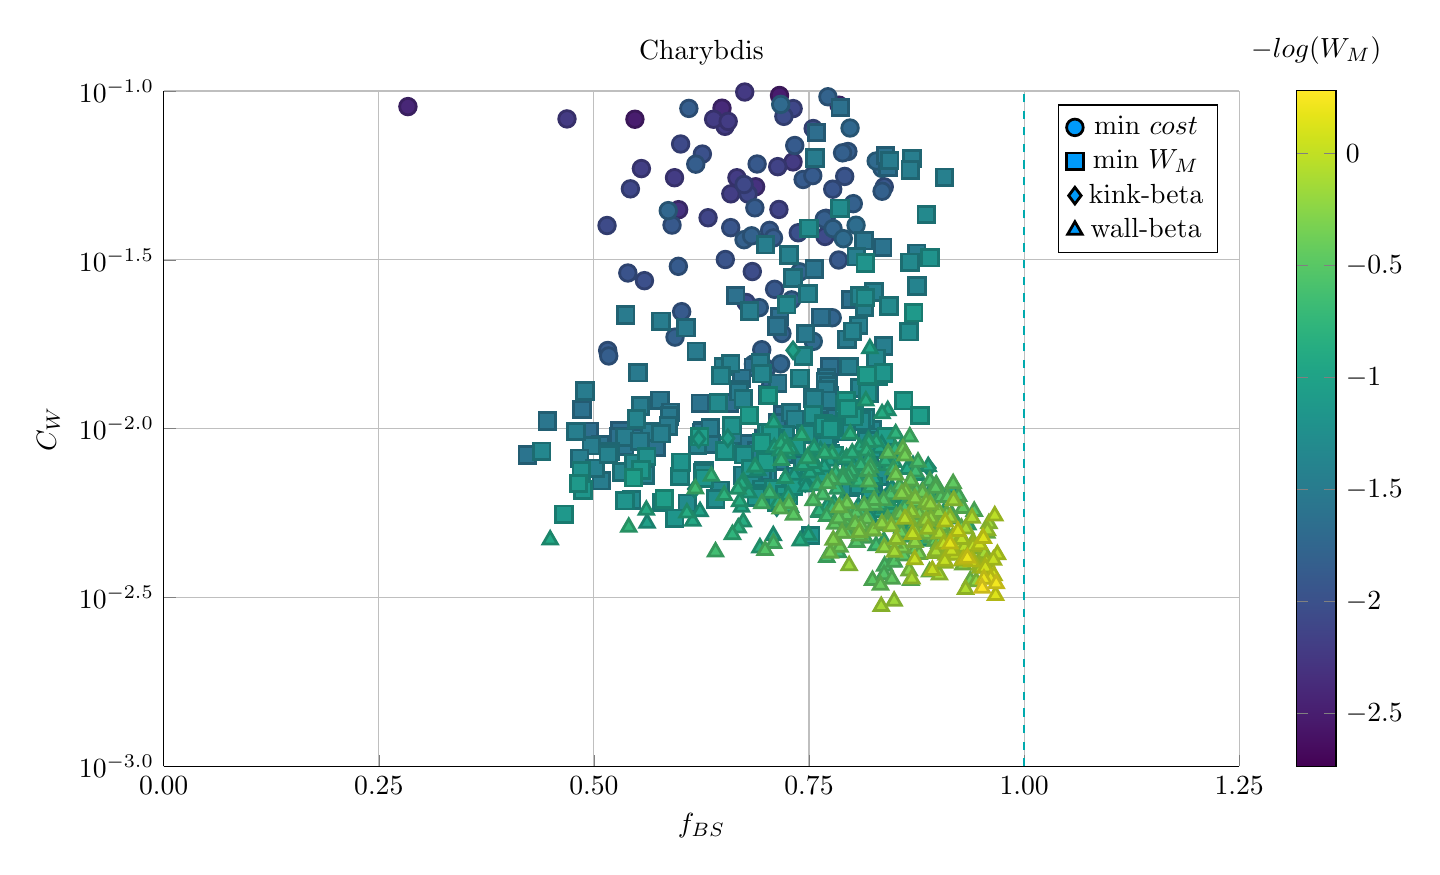
\begin{tikzpicture}[]
\begin{axis}[colorbar = {true}, height = {101.6mm}, ylabel = {${C}_{W}$}, title = {Charybdis}, xmin = {0.0}, xmax = {1.25}, ymax = {0.1}, ymode = {log}, xlabel = {${f}_{BS}$}, {unbounded coords=jump, scaled x ticks = false, xticklabel style={rotate = 0}, xmajorgrids = true, xtick = {0.0,0.25,0.5,0.75,1.0,1.25}, xticklabels = {0.00,0.25,0.50,0.75,1.00,1.25}, xtick align = inside, axis lines* = left, scaled y ticks = false, yticklabel style={rotate = 0}, log basis y=10, ymajorgrids = true, ytick = {0.001,0.0031622776601683794,0.01,0.03162277660168379,0.1}, yticklabels = {$10^{-3.0}$,$10^{-2.5}$,$10^{-2.0}$,$10^{-1.5}$,$10^{-1.0}$}, ytick align = inside, axis lines* = left,     xshift = 0.0mm,
    yshift = 0.0mm,
    axis background/.style={fill={rgb,1:red,1.00000000;green,1.00000000;blue,1.00000000}}
, colormap={plots}{rgb=(0.26700400,0.00487400,0.32941500), rgb=(0.27794100,0.05632400,0.38119100), rgb=(0.28291000,0.10539300,0.42690200), rgb=(0.28229000,0.14591200,0.46151000), rgb=(0.27619400,0.19007400,0.49300100), rgb=(0.26514500,0.23295600,0.51659900), rgb=(0.25042500,0.27429000,0.53310300), rgb=(0.23360300,0.31382800,0.54391400), rgb=(0.21813000,0.34743200,0.55003800), rgb=(0.20123900,0.38367000,0.55429400), rgb=(0.18555600,0.41857000,0.55675300), rgb=(0.17117600,0.45253000,0.55796500), rgb=(0.15772900,0.48593200,0.55801300), rgb=(0.14618000,0.51541300,0.55682300), rgb=(0.13374300,0.54853500,0.55354100), rgb=(0.12346300,0.58168700,0.54744500), rgb=(0.11948300,0.61481700,0.53769200), rgb=(0.12632600,0.64410700,0.52531100), rgb=(0.15014800,0.67663100,0.50658900), rgb=(0.19109000,0.70836600,0.48228400), rgb=(0.24607000,0.73891000,0.45202400), rgb=(0.31192500,0.76782200,0.41558600), rgb=(0.37777900,0.79178100,0.37793900), rgb=(0.45867400,0.81636300,0.32972700), rgb=(0.54552400,0.83803900,0.27562600), rgb=(0.63690200,0.85654200,0.21662000), rgb=(0.73088900,0.87191600,0.15602900), rgb=(0.81457600,0.88339300,0.11034700), rgb=(0.90631100,0.89485500,0.09812500), rgb=(0.99324800,0.90615700,0.14393600)}, colorbar style={title=$-log( W_M )$}}, ymin = {0.001}, width = {152.4mm}]\addplot+[scatter, scatter src=explicit, only marks = {true}, color = {rgb,1:red,0.00000000;green,0.60560316;blue,0.97868012},
draw opacity=1,
line width=0,
solid,mark = *,
mark size = 3.0,
mark options = {
    color = {rgb,1:red,0.00000000;green,0.00000000;blue,0.00000000}, draw opacity = 1.0,
    fill = {rgb,1:red,0.00000000;green,0.60560316;blue,0.97868012}, fill opacity = 1,
    line width = 1,
    rotate = 0,
    solid
}] coordinates {
(0.7359024750431782, 0.20372611777337152) [-2.737608795379803]
(0.5851953957160873, 0.16756698485075783) [-2.687028959846787]
(0.5364581048179937, 0.20307732356386315) [-2.590964172611572]
(0.7157155795294491, 0.09697011319422226) [-2.5133293798402634]
(0.5476668344586882, 0.08246486806905176) [-2.5100019193902536]
(0.5752437728161253, 0.19848215388453824) [-2.5025824444647777]
(0.7822657902821669, 0.18469850991270712) [-2.5011605733960924]
(0.7330176082872631, 0.12156262800516612) [-2.487146433631915]
(0.6068870363747878, 0.19851381203738652) [-2.4809660057819647]
(0.6590347940805605, 0.18516332132320687) [-2.470276837036607]
(0.2838228884486824, 0.08989325143911144) [-2.4120510478783452]
(0.5708561611145753, 0.11208716242840429) [-2.40064821683863]
(0.6846120659221104, 0.1197463715660703) [-2.3953673323479805]
(0.4540491134456154, 0.16126185747296792) [-2.393026566903574]
(0.664870722620742, 0.12157790627296668) [-2.3890711431592075]
(0.6488772614768177, 0.08892691625963052) [-2.3841714318705525]
(0.7962903980838778, 0.19098420146344375) [-2.3835230043455686]
(0.5527152139738948, 0.1567069747417994) [-2.381290315955617]
(0.5688566985496978, 0.12013460973440174) [-2.372431680776573]
(0.7534891693764634, 0.18909730733563926) [-2.3528250340145016]
(0.7848680602764574, 0.09075329244454268) [-2.3367870360584306]
(0.6786405769951752, 0.14161197175057597) [-2.321478568273318]
(0.6879316398295171, 0.05204568902739023) [-2.305558880403713]
(0.6025332208962126, 0.12356138844469775) [-2.304074016625784]
(0.5984321265445931, 0.04451265485552352) [-2.302767677581907]
(0.7386606591169115, 0.16063854506387298) [-2.296827704935537]
(0.6511502088521184, 0.10163604971512134) [-2.2875898578722627]
(0.7194233620171044, 0.11621384520807569) [-2.277792210835674]
(0.7567514313688793, 0.1663671711858832) [-2.2429196737605452]
(0.7579186381402687, 0.14065371048755002) [-2.2307023150334016]
(0.6752700403564966, 0.0992781716492562) [-2.229928759421221]
(0.7314415782128092, 0.06165765133592798) [-2.225497521252979]
(0.4687064864215902, 0.08264995845897197) [-2.2254079847151558]
(0.798488185414572, 0.10066936171865973) [-2.2222117952587324]
(0.7999537680483143, 0.11283696845057267) [-2.2164511971368666]
(0.6523833432801946, 0.07858675141449649) [-2.209080463460292]
(0.5936775460828698, 0.055353669168383704) [-2.209072102647127]
(0.639129584480767, 0.08246628156983182) [-2.2082284492074966]
(0.666208795279778, 0.05534045927382465) [-2.207545754633005]
(0.6560427480245121, 0.0812523499942961) [-2.2073960717358423]
(0.6591405401085446, 0.04959003498021099) [-2.1906798686881843]
(0.5551837247381063, 0.058916370946488036) [-2.180354292184896]
(0.7150132537788763, 0.04458441983079472) [-2.1445063804884623]
(0.7136491796753617, 0.05969099272190574) [-2.1441459472897755]
(0.6326692663477658, 0.04213154094480493) [-2.1211539010866085]
(0.7506892183015275, 0.11416954810746238) [-2.118865769548717]
(0.6791864978600942, 0.04953083435602705) [-2.0989534800462293]
(0.7315469652365952, 0.08867461574773429) [-2.098220502653117]
(0.6745347277267081, 0.0528553369774306) [-2.0935531757786148]
(0.5424055033322877, 0.05131047258257683) [-2.0908793980048204]
(0.6007799858607985, 0.06966107994211436) [-2.071206080374841]
(0.5152474997516242, 0.03996425224364798) [-2.064010547202469]
(0.7686026115092387, 0.03708750697043753) [-2.056677518407323]
(0.7207865714460837, 0.08410248770893317) [-2.046651526754166]
(0.6840849685675889, 0.029196081498388402) [-2.0379011758864283]
(0.7548350354881133, 0.07740613615195041) [-2.0346098603711273]
(0.6768336159103454, 0.023645385119135078) [-2.0286798881208097]
(0.5587072189827298, 0.027435451545116674) [-2.0136110022221563]
(0.7350235456977134, 0.11225395679162868) [-2.009422091461703]
(0.7375305044186223, 0.038038514881495206) [-2.0046094254929896]
(0.626054073537986, 0.06504727548043324) [-1.9998626026906214]
(0.5912300263829029, 0.1292818470624988) [-1.994011891463306]
(0.5394375501946231, 0.028908830411030862) [-1.9684875514336135]
(0.6527344577201069, 0.031694615819844695) [-1.962505769886516]
(0.7698840234200133, 0.041976164443053174) [-1.9620022465602456]
(0.7914883153195793, 0.0558374666834525) [-1.9556964151982232]
(0.7775684313579326, 0.051180643617204404) [-1.951439472922028]
(0.658985769190255, 0.03938689654476367) [-1.9407104232831573]
(0.8374522478389551, 0.05202238389928039) [-1.9285131737739916]
(0.7100254506306457, 0.025864965787053298) [-1.9158089273231942]
(0.7844213227435214, 0.0315876708787529) [-1.9026235632381945]
(0.5907921919303644, 0.04007799426592172) [-1.8998797107494547]
(0.6896895825351187, 0.06078277028813781) [-1.899469008660825]
(0.6019792525002452, 0.022206649532263138) [-1.8922403969034376]
(0.6914159704451317, 0.10343738795419383) [-1.8906275193753241]
(0.7041896502823766, 0.03865878413437627) [-1.888904730447693]
(0.5160181017136422, 0.01704724215883986) [-1.881726038777211]
(0.743187295487432, 0.05468787224768575) [-1.8763775212700056]
(0.7334309591956334, 0.06894730353059726) [-1.8735628617782005]
(0.5981394027328019, 0.030255781340376833) [-1.8728583861908288]
(0.7543798247443579, 0.05616340524751281) [-1.8726476950037667]
(0.6870514960504185, 0.04508699905590542) [-1.8707673950160981]
(0.7087125757213878, 0.036730885786441146) [-1.8559040168248113]
(0.6183905781152413, 0.06072120698828991) [-1.844735439552174]
(0.6103504198051167, 0.0887876180917983) [-1.8430067319432535]
(0.7951817179395599, 0.06618962633184258) [-1.8418706711323614]
(0.5172145933348372, 0.016421469596061083) [-1.839654971931263]
(0.7677643488639188, 0.041749778425302704) [-1.8363695553529753]
(0.6950647568960668, 0.017133631996777206) [-1.8261042714032643]
(0.7890113216319079, 0.06559232169922954) [-1.8156007183182272]
(0.8349557353351424, 0.050477285906930965) [-1.814915147975814]
(0.8014700349403633, 0.0463768454249938) [-1.8142470512570916]
(0.6922025322322042, 0.022826470712123872) [-1.8122133933822206]
(0.5942649107552632, 0.018671308945999422) [-1.8120480447424478]
(0.7298578035996299, 0.02406843511337114) [-1.810457309558868]
(0.6744865705831616, 0.03627504764978015) [-1.8068853182048894]
(0.7185012463149602, 0.019138039216325595) [-1.8019457667366159]
(0.6832930480165496, 0.03724912279904193) [-1.7968505393892884]
(0.7007625467971873, 0.015068032824050809) [-1.7952329403066731]
(0.8529644136574135, 0.10460346899306477) [-1.7847262081815998]
(0.7719812027452927, 0.09611727933154134) [-1.7840094275762153]
(0.7769681596557587, 0.021310065419317785) [-1.76773605949338]
(0.7393128324823182, 0.02913495659310822) [-1.7643358761825505]
(0.7056419712157331, 0.013537430460188857) [-1.7636964772599824]
(0.7169853719943156, 0.015563838196545969) [-1.7631697711543228]
(0.7779068969066241, 0.039135813481222324) [-1.7625125196445544]
(0.8348226277408363, 0.058991966200443106) [-1.7573515468471756]
(0.5863935693560001, 0.04422563848495237) [-1.7287980416000448]
(0.7977038871187261, 0.07767888704178068) [-1.7234251960549989]
(0.8280920948475081, 0.06204137364185275) [-1.706346162862732]
(0.7549772489845689, 0.018138423087163798) [-1.7045486732225623]
(0.7171125889592607, 0.09124971330207729) [-1.7014359592573747]
(0.7899075292932638, 0.0365316783828158) [-1.6927990438723723]
(0.6853958214714885, 0.015536674756802697) [-1.6898457437353114]
(0.804693703903259, 0.04003550886686569) [-1.6732846842044926]
};
\addlegendentry{min $cost$}
\addlegendentry{min $W_M$}
\addlegendentry{kink-beta}
\addlegendentry{wall-beta}
\addplot+[scatter, scatter src=explicit, only marks = {true}, color = {rgb,1:red,0.00000000;green,0.60560316;blue,0.97868012},
draw opacity=1,
line width=0,
solid,mark = square*,
mark size = 3.0,
mark options = {
    color = {rgb,1:red,0.00000000;green,0.00000000;blue,0.00000000}, draw opacity = 1.0,
    fill = {rgb,1:red,0.00000000;green,0.60560316;blue,0.97868012}, fill opacity = 1,
    line width = 1,
    rotate = 0,
    solid
}] coordinates {
(0.6851210809340392, 0.015197399614753464) [-1.6681264025020264]
(0.4941964393824304, 0.009823451646161325) [-1.663027891651841]
(0.530160434168107, 0.009846202245989184) [-1.6574639825902946]
(0.657378449413485, 0.011920058291303071) [-1.6569597902573525]
(0.7586216148428655, 0.07535163980234072) [-1.6567719329389001]
(0.7158310476944133, 0.02145281320442147) [-1.6490985707391912]
(0.7192558858327268, 0.010980468278747128) [-1.6422304847233504]
(0.7981807918170106, 0.024120165421292625) [-1.6325751861823363]
(0.7640459388499986, 0.021369208393676346) [-1.6291941426087102]
(0.8417754201260752, 0.059322254561326254) [-1.6271960977249518]
(0.7743051372156727, 0.015274978962504819) [-1.6270750467611084]
(0.664700618113425, 0.02479273110440336) [-1.626888156587228]
(0.7863682794539396, 0.08930149237460469) [-1.6249314455189936]
(0.5291119244133525, 0.009464726031912818) [-1.616950986036806]
(0.48595797227950854, 0.01140193486941599) [-1.6155813119347568]
(0.5723299817732307, 0.008812988458667981) [-1.6136190879018757]
(0.8388405409449038, 0.06439016913414505) [-1.6120765470743166]
(0.70226409417234, 0.012585512817446045) [-1.6084381516776733]
(0.7130021869125045, 0.02012839274260647) [-1.6020711217447665]
(0.5077104629720907, 0.008960652359910951) [-1.5956625490662]
(0.623540667348531, 0.011885919211945236) [-1.5936419030965376]
(0.8357083811774292, 0.03445722055743375) [-1.591719437101271]
(0.6974358183207425, 0.00935259758229712) [-1.5882416690043395]
(0.5494745058252606, 0.00941739351173858) [-1.587943800614445]
(0.4225576148062277, 0.008359730036220061) [-1.5878025494857624]
(0.7131882171897006, 0.010419937829338555) [-1.5868755906181577]
(0.7562368917045845, 0.029697190504060857) [-1.5849823271963874]
(0.6716640548925399, 0.014090253789926491) [-1.5820661333237485]
(0.6267086866070536, 0.009872769680224545) [-1.571414774494934]
(0.8140161912399068, 0.036055486397936085) [-1.561587842338199]
(0.6792373315387156, 0.009008401602884603) [-1.5604752308741954]
(0.44591630111536584, 0.010548811329102839) [-1.560024208321792]
(0.6253833131119283, 0.00975086483062938) [-1.5595172183929409]
(0.5357717637014691, 0.008877515881031174) [-1.5547403592804268]
(0.5767804998324492, 0.012128004524771618) [-1.5525172912757694]
(0.7804693216914177, 0.01075120106159998) [-1.550211325130473]
(0.7706256099884414, 0.01417054313300387) [-1.5499921130488996]
(0.7136233520662059, 0.013636547782905628) [-1.5488389310082484]
(0.5890435534060732, 0.01118682853182229) [-1.548636584215126]
(0.6960995570081354, 0.009004515948176011) [-1.5484303677563682]
(0.6891089745706832, 0.008589361734950092) [-1.5300696832010154]
(0.5877673649863151, 0.010918478084483) [-1.5240418415006989]
(0.7689373516155897, 0.013786535741271849) [-1.52035115860342]
(0.7458916933725457, 0.019102159289939535) [-1.5187095286365286]
(0.607104129340485, 0.019900882686515825) [-1.5152558703618486]
(0.7547906590532093, 0.01233142370653334) [-1.5130633149050525]
(0.6362345823351421, 0.008998649144966384) [-1.5127417843169062]
(0.727050378229241, 0.009033035828776036) [-1.512065872282441]
(0.5513544713967212, 0.014648425212785676) [-1.508698938344436]
(0.5368536810825235, 0.021717369003602268) [-1.5042599211378067]
(0.7620316566255821, 0.011787983533386965) [-1.5034350531454859]
(0.7725639125650813, 0.013402736400337721) [-1.50170709764633]
(0.681235287648052, 0.008403497514698337) [-1.501622468932281]
(0.6691676415273751, 0.013038942564365743) [-1.5014482706318735]
(0.7939788263529484, 0.018390392389316428) [-1.4999954524234758]
(0.6189955986913707, 0.01694354359189593) [-1.4973617780251773]
(0.5863662794504805, 0.010183371556613061) [-1.497105465512374]
(0.8436473841822292, 0.062282935043912684) [-1.4929511344473714]
(0.7571308398620893, 0.06324187033686292) [-1.4921349419619385]
(0.7738151286426059, 0.012548762978995496) [-1.4884591559674822]
(0.6686415918300896, 0.012867101009559307) [-1.487363796795517]
(0.4895966961882071, 0.012921001622500157) [-1.4866917975345906]
(0.6353463643428903, 0.010047951074758055) [-1.4840978906845892]
(0.8751665097475697, 0.03303866433608294) [-1.4824521913249147]
(0.8201318460604853, 0.012726704506142847) [-1.4821332841886103]
(0.5495938989749863, 0.007290805739373347) [-1.48122389777201]
(0.5651448258793007, 0.00977012454088988) [-1.4804970319589599]
(0.5085409731766444, 0.007020834402326414) [-1.4800609203732897]
(0.497047495750633, 0.008910343679206711) [-1.4785263901161534]
(0.7700846921982628, 0.013060328514041545) [-1.4759327339004988]
(0.6613546957182095, 0.009568901799246174) [-1.4716802129865878]
(0.5541661197172657, 0.011686646580567617) [-1.4714171457200942]
(0.5357853528313937, 0.009432683201513142) [-1.4697490463241623]
(0.5780574343855402, 0.0207896268155257) [-1.469182095495403]
(0.749496638108765, 0.00970055448692835) [-1.4669160574764228]
(0.7750171669992052, 0.009906198335664992) [-1.4650279037766998]
(0.48334514281038826, 0.008175296861755412) [-1.4649157170050158]
(0.8695060800287956, 0.06304537805517052) [-1.4637589731711664]
(0.8678168316150046, 0.058293696935902015) [-1.4637269213699509]
(0.6810497144003721, 0.022332692478256824) [-1.4633431723635995]
(0.553769872193598, 0.009175072172052877) [-1.4625771233357587]
(0.6993360633065318, 0.03507245292213848) [-1.4624493219359893]
(0.8048754097940412, 0.0323252483349636) [-1.456137936078477]
(0.7724185214963187, 0.012144991566364045) [-1.4552956920106896]
(0.47939065080719445, 0.009807429458519862) [-1.4545765412204814]
(0.83685598069093, 0.017552109366812733) [-1.4536933205355047]
(0.7008512611510139, 0.008376880643338882) [-1.4536264367612777]
(0.7313032608836818, 0.027928446404318328) [-1.4522195766945736]
(0.7965110041064016, 0.015275332383460013) [-1.4474663709891824]
(0.6932958919872281, 0.015700047070746036) [-1.4473086055649607]
(0.7730881776814797, 0.009670159078421467) [-1.4394573389116623]
(0.5779570147935796, 0.00966580645268258) [-1.43910869750835]
(0.8078038051086585, 0.02020398851625505) [-1.4359212547397637]
(0.715499444782145, 0.008025741974410725) [-1.4345455569874563]
(0.7208841307372137, 0.008395971364345037) [-1.4342039611389994]
(0.9074238589733309, 0.055516720625521446) [-1.431939711468657]
(0.5190051987619015, 0.008564631451482608) [-1.4318393301192203]
(0.6504475928061844, 0.015286328537971657) [-1.4298782830268841]
(0.7292085089618878, 0.011144326549623773) [-1.4297531319990848]
(0.81448792065999, 0.022836013108600235) [-1.429493152311542]
(0.825574988161768, 0.02541733792453219) [-1.4257656907023994]
(0.501465121842191, 0.007637958943877289) [-1.4246908118870814]
(0.7266226606300097, 0.032702505993041836) [-1.4223151615986427]
(0.6591067142233716, 0.015605848032644089) [-1.4209285260987674]
(0.5167081891349604, 0.00838874188644035) [-1.4103191250155003]
(0.5596505617132486, 0.007287678962320866) [-1.409160412241362]
(0.7557455862541304, 0.012263516831132143) [-1.3987487890322283]
(0.7341248325017325, 0.010656632838165833) [-1.3961077718749653]
(0.8092287508171119, 0.013186567390631069) [-1.39553831950318]
(0.8203576874800285, 0.00805251109990194) [-1.3921916689745937]
(0.8004943813587586, 0.019423304332311736) [-1.391977480132208]
(0.7489120391350832, 0.025114205055596032) [-1.3910450519688433]
(0.8754057461611234, 0.026458278303411537) [-1.3854794296349102]
(0.6735716252835262, 0.012247975078154037) [-1.3835251244626703]
(0.7665028038099523, 0.008921077760690099) [-1.3812630274600655]
(0.7015621857164597, 0.007416332681742631) [-1.3791460184166777]
(0.6202964877938695, 0.008932161350486465) [-1.376877777579119]
(0.8087590580422906, 0.024683476432383993) [-1.375791428631395]
(0.5494124765358024, 0.010670268336180793) [-1.3747828318073587]
(0.8149159088702812, 0.007870433585163046) [-1.3692376523933565]
(0.5320990994872573, 0.0074378152848894735) [-1.3684330757581267]
(0.7481734016173558, 0.008098566001726598) [-1.3642308788975135]
(0.6476576358282994, 0.014345667909698757) [-1.3639106630352087]
(0.6558906704773511, 0.008572986953587419) [-1.3552608297970883]
(0.8237471775593819, 0.00992037446225701) [-1.3550143961305745]
(0.7982100921053328, 0.007328347073490059) [-1.3536632792649093]
(0.6953629282134552, 0.007510901593863939) [-1.3520272957429909]
(0.6953230050470768, 0.014541602438699657) [-1.3510576974042412]
(0.6730211677715083, 0.007284218364658594) [-1.3496042220443973]
(0.7239679168228259, 0.023274179527198832) [-1.341589260669594]
(0.4393956478215161, 0.008576558289309913) [-1.3400141478767358]
(0.7426807786520446, 0.00783880949696723) [-1.3300314493551002]
(0.7395236873382182, 0.01411038207207742) [-1.3284263237560021]
(0.684855303548374, 0.007486503783717723) [-1.3242939338468662]
(0.8278021824532116, 0.016172436730796002) [-1.323178727777929]
(0.627797840186422, 0.007515284989600465) [-1.3213550729926942]
(0.8674653533336951, 0.031083172357107024) [-1.3188753969554132]
(0.6467532218081451, 0.006572813918743706) [-1.3138992633454782]
(0.8864160782387862, 0.04309583371292883) [-1.3112533972207423]
(0.6269156989625477, 0.007413444843148486) [-1.3066175516543825]
(0.8431393595924693, 0.02306836377257982) [-1.3040612288627607]
(0.8197076367002643, 0.00943254285754032) [-1.3038133693852783]
(0.6445239701337245, 0.01190899263404481) [-1.301084703290134]
(0.5463650306744098, 0.00789699984651379) [-1.3010145120900876]
(0.5437906828898529, 0.006149219434619409) [-1.3000605956773916]
(0.7434166628060613, 0.016437005811172183) [-1.2981699890610565]
(0.7146749298387812, 0.008660055713531614) [-1.2951558801969907]
(0.8148780528301931, 0.010749954823506654) [-1.29444309797184]
(0.6084531928479563, 0.006015009649024556) [-1.2856101424882644]
(0.7220256115514188, 0.009584357937856927) [-1.285263592011844]
(0.7859463410460376, 0.04494124949431044) [-1.284383793501614]
(0.799675832204197, 0.00683431321635412) [-1.2828114288158374]
(0.7499713034119133, 0.039187382342347976) [-1.2826431650359629]
(0.734351532241878, 0.007231700278305266) [-1.2824255065429995]
(0.713445223919135, 0.00853616645957665) [-1.2813323109549335]
(0.790122159696273, 0.006837657402697755) [-1.2806421539894215]
(0.8175324002405339, 0.009211465915111147) [-1.2790915578265545]
(0.8109413385537045, 0.010542099378207213) [-1.2707451840708122]
(0.8154085690878763, 0.024447750750697092) [-1.2676539939434082]
(0.771441058879269, 0.009098409772603787) [-1.2653553126366786]
(0.7976978951094078, 0.006725537497980498) [-1.264293982211982]
(0.8663731578909948, 0.019363431367524053) [-1.262045130852001]
(0.6826626081076077, 0.006906076996276599) [-1.2611290819783112]
(0.7930953306749782, 0.009803145458874337) [-1.2555987795426622]
(0.6414699980625864, 0.00619895569247597) [-1.2513270179335647]
(0.8316118369664839, 0.007239853513876978) [-1.2453167838780697]
(0.7681268084076656, 0.008896586162085272) [-1.2430939343579344]
(0.7009518612475429, 0.009719593902466845) [-1.2381773742332136]
(0.5613695492397395, 0.008270424440644015) [-1.2346782486332617]
(0.60010992732849, 0.0072241626571935376) [-1.2264046023709216]
(0.7548991538536438, 0.01098843719538726) [-1.2247195887884887]
(0.7269708164874584, 0.006808974225612837) [-1.2180889658059086]
(0.6946997618970708, 0.006611305121542242) [-1.2173874089477876]
(0.48544389569163865, 0.007501419726936573) [-1.2146247722956514]
(0.7909335635528599, 0.011764386053045915) [-1.2132972156104522]
(0.6745620250506631, 0.008378063320530003) [-1.2109120215395388]
(0.7747592904603993, 0.008427299987451904) [-1.2084181738286368]
(0.8180761130344034, 0.01273555061242485) [-1.20714909048448]
(0.6600048470179246, 0.010213320377511352) [-1.2033520253557135]
(0.8904893803598241, 0.032086426450625864) [-1.1973567207367808]
(0.7794460337871526, 0.01024990923611188) [-1.1946911954531152]
(0.7685171934523852, 0.010020735618058307) [-1.194687477055283]
(0.74643037518658, 0.009634752809511687) [-1.1937967228670217]
(0.8305632837722567, 0.014319974319254046) [-1.185724861965876]
(0.8154688896102296, 0.030946696104817876) [-1.1815951507377263]
(0.5359199492602275, 0.006119538485938838) [-1.1806237088701466]
(0.5790003431047352, 0.0060467130253046425) [-1.1800813312023146]
(0.6010234873787892, 0.007952378649071718) [-1.176244530950471]
(0.6903543708921169, 0.006432608194369421) [-1.1748225292203367]
(0.5938066341086683, 0.005427058328431804) [-1.1721208310483742]
(0.8244672749127927, 0.006744537821609478) [-1.1717373686057835]
(0.7520366981220118, 0.004828891223049449) [-1.1708649361692889]
(0.8079347587629624, 0.006810003648499363) [-1.1692163263768098]
(0.7113020735368382, 0.009353534353065332) [-1.167353919317699]
(0.8366541770603382, 0.014618785296867573) [-1.1652399164280889]
(0.8261711137782428, 0.008829535690276422) [-1.162809974145342]
(0.6281137770625854, 0.007136024429485349) [-1.1600693635040116]
(0.48744515553761025, 0.006579111152003091) [-1.157321108695414]
(0.651991884299557, 0.008599780741533768) [-1.1572067562856314]
(0.7107092242352311, 0.009251618906581017) [-1.1571634670399211]
(0.8088839694703398, 0.008133610271699837) [-1.154357334346231]
(0.8027929243249681, 0.011084851654264415) [-1.1506586644938104]
(0.823695688879586, 0.008713510430388705) [-1.150227655836216]
(0.822008562445382, 0.006602548762005154) [-1.1491924102402016]
(0.688612348505278, 0.006272419326365313) [-1.1477835171917188]
(0.6820414615312915, 0.007620679601131938) [-1.1465058315496728]
(0.7665548771358827, 0.010377192915174936) [-1.145014274974487]
(0.705868708485792, 0.009696220536212618) [-1.1375870233869183]
(0.767634347550663, 0.010180634102852183) [-1.1373650551215082]
(0.5547128257478453, 0.007542730978334406) [-1.1357458790371815]
(0.7783986920955023, 0.010126349397671063) [-1.133986432515703]
(0.4651362590200956, 0.005578205050921048) [-1.1320341014158335]
(0.8015228446950137, 0.010846318354017281) [-1.127079592692178]
(0.726461760542858, 0.006331906889150134) [-1.1252988863479554]
(0.48208147962640285, 0.006879141460401252) [-1.123003263844327]
(0.8717607864580118, 0.022040928898795047) [-1.1207682191899027]
(0.774982528534528, 0.00996173564893061) [-1.1180749050851169]
(0.7093096094323664, 0.006626896988025552) [-1.1159299024060154]
(0.8171791685966094, 0.014399132022875615) [-1.111366047368976]
(0.7932954390046818, 0.01206983625295502) [-1.1093461418096882]
(0.7219772506321358, 0.006356432017833017) [-1.1083223146390213]
(0.7029191591245791, 0.012535144034281957) [-1.108020004377878]
(0.7346977255426123, 0.00883860338226376) [-1.1055395253528022]
(0.6805779282507709, 0.010954609847675004) [-1.1018087579792433]
(0.7375539791268741, 0.006955673427821012) [-1.1000312304906807]
(0.7953037368390077, 0.011476323196829152) [-1.0958683903566835]
(0.8599427472738629, 0.012099180088161502) [-1.0918611830445206]
(0.7644072104571058, 0.007324655445979312) [-1.084008635561983]
(0.779650226067546, 0.008347799057721199) [-1.0818442729737123]
(0.6998274928068458, 0.007973263522900845) [-1.0762205003226006]
(0.87917336532856, 0.010946001598484297) [-1.0742112770850791]
(0.694879746234392, 0.009087852412631436) [-1.0708769548182164]
(0.7321698469384964, 0.0067597442860644836) [-1.069695292943837]
(0.545938699421471, 0.007160447099405331) [-1.0603710996179994]
(0.6228473762742924, 0.009473258949863166) [-1.058639833713732]
(0.5819104753803194, 0.0061899243692649306) [-1.0559914680496412]
(0.8398342477938563, 0.009482529791919412) [-1.0537452246128203]
(0.7506931030637808, 0.00708059455566661) [-1.0532767994986825]
(0.7126332937977515, 0.006035560775312132) [-1.0518252532905286]
};
\addlegendentry{min $cost$}
\addlegendentry{min $W_M$}
\addlegendentry{kink-beta}
\addlegendentry{wall-beta}
\addplot+[scatter, scatter src=explicit, only marks = {true}, color = {rgb,1:red,0.00000000;green,0.60560316;blue,0.97868012},
draw opacity=1,
line width=0,
solid,mark = diamond*,
mark size = 3.0,
mark options = {
    color = {rgb,1:red,0.00000000;green,0.00000000;blue,0.00000000}, draw opacity = 1.0,
    fill = {rgb,1:red,0.00000000;green,0.60560316;blue,0.97868012}, fill opacity = 1,
    line width = 1,
    rotate = 0,
    solid
}] coordinates {
(0.834626495849728, 0.006083501631057066) [-1.0496814932160978]
(0.6170409460102284, 0.006629793134010975) [-1.0478282176510978]
(0.8894694614486488, 0.00764908073743482) [-1.0476862508436227]
(0.7124945816098436, 0.005862884354721373) [-1.0434060376287386]
(0.6218172305989085, 0.009322710512378526) [-1.042586757918211]
(0.8441447569005192, 0.006487752068877104) [-1.0395059774095508]
(0.6555943522609418, 0.009374281366493263) [-1.037130039873791]
(0.7314329599011424, 0.0170614588554745) [-1.0308313508546258]
(0.745698806783015, 0.006913114243597262) [-1.0275590312193816]
};
\addlegendentry{min $cost$}
\addlegendentry{min $W_M$}
\addlegendentry{kink-beta}
\addlegendentry{wall-beta}
\addplot+[scatter, scatter src=explicit, only marks = {true}, color = {rgb,1:red,0.00000000;green,0.60560316;blue,0.97868012},
draw opacity=1,
line width=0,
solid,mark = triangle*,
mark size = 3.0,
mark options = {
    color = {rgb,1:red,0.00000000;green,0.00000000;blue,0.00000000}, draw opacity = 1.0,
    fill = {rgb,1:red,0.00000000;green,0.60560316;blue,0.97868012}, fill opacity = 1,
    line width = 1,
    rotate = 0,
    solid
}] coordinates {
(0.561781693172161, 0.005256053052710575) [-1.025114084474608]
(0.7328778253267054, 0.007284527271346537) [-1.025064662372027]
(0.8007534210560534, 0.00782078493256419) [-1.0135716419780334]
(0.8262131393427226, 0.005878041854646887) [-1.0133032391552028]
(0.6905506855070277, 0.007516810149579491) [-1.0129395602075102]
(0.8321644284749603, 0.005642606316680264) [-1.0090683465802397]
(0.7950726411527982, 0.007590586049588419) [-1.00487994972194]
(0.7745441322154459, 0.008018904893245096) [-1.0024486517409639]
(0.6233290112259804, 0.005687012650490601) [-0.9982503197852052]
(0.8207534028698369, 0.017272851302606376) [-0.9980863049007114]
(0.8345152086201154, 0.008976011549139531) [-0.9976413099828907]
(0.7463634982112085, 0.00672377146821775) [-0.9952427135597887]
(0.8372618582030043, 0.006179152610909006) [-0.9882704184280687]
(0.8464783361909116, 0.006658577387207133) [-0.9865959618907963]
(0.7633220600898417, 0.008611185683760977) [-0.9861502224644026]
(0.7552278550565529, 0.00861006159819778) [-0.9834884062410291]
(0.8264185188855481, 0.007078972975952707) [-0.9755470230412873]
(0.7923915340714205, 0.007165169234302644) [-0.9751682968759733]
(0.8074567550650718, 0.00588288059860778) [-0.9745460269854277]
(0.8318914609825181, 0.008762707263760248) [-0.9724510296030006]
(0.8213035185218059, 0.0054508764537053) [-0.9721723790112873]
(0.7930318484620907, 0.007500206088288035) [-0.9683079871351761]
(0.8188945200120549, 0.00925430650881406) [-0.9640479639625688]
(0.767842670848498, 0.007713542274813112) [-0.9605456904465843]
(0.7096157753674764, 0.008793232884908199) [-0.9509475064598062]
(0.7580155421129163, 0.00758530046831779) [-0.9475613034981963]
(0.7089024870209081, 0.010432599107525612) [-0.9431073279051986]
(0.9149131868692663, 0.006669463740427501) [-0.9395228095882537]
(0.4491718650706183, 0.004688262944849126) [-0.9379797386819722]
(0.6716296429821872, 0.005855680709409532) [-0.936956260188316]
(0.7084973783953123, 0.004823068577046762) [-0.9328401416066296]
(0.8473084623363518, 0.006257853989784519) [-0.9307108052550614]
(0.680102277451425, 0.006461854726339168) [-0.9281558619803609]
(0.7286173554216664, 0.008735963170322575) [-0.9264995775599043]
(0.6148265392179618, 0.005328057424477724) [-0.9262426999191099]
(0.8708623476098649, 0.007790932759723544) [-0.9227003718927437]
(0.7511842078366924, 0.007406866683715918) [-0.9211202387251416]
(0.7492906727437184, 0.004842693465206878) [-0.9122780994598872]
(0.7955701829594555, 0.00553456744660005) [-0.9098639973117462]
(0.7558381020157489, 0.00799774423691871) [-0.9085892171866993]
(0.8415001071316417, 0.011322447729645281) [-0.9043705523492929]
(0.7890506006382549, 0.008178982728725071) [-0.903352069757217]
(0.7712915128293827, 0.0058981820527739225) [-0.9005612951337819]
(0.7258140216436932, 0.006353815969057234) [-0.8985196847828957]
(0.5609209176660367, 0.005739892493181049) [-0.8983797144291398]
(0.8639203180223186, 0.007583618995886536) [-0.8971261027713628]
(0.8607562916265183, 0.006081355532545074) [-0.8962149920198969]
(0.754373466724369, 0.007895141300507174) [-0.8947574466288085]
(0.7247460265098778, 0.008446442250875192) [-0.8916300803179569]
(0.8160520408511582, 0.012086236110976131) [-0.890947883956792]
(0.8885362197506304, 0.007728598763745398) [-0.8865999168444305]
(0.6739713276486742, 0.006968625853256571) [-0.8862290860463612]
(0.6718514222391598, 0.00686791587727973) [-0.8853692596179883]
(0.8349391514029897, 0.011077289150155845) [-0.884029767456243]
(0.8386840624601364, 0.005982150284429834) [-0.8837850767800522]
(0.7926189511510549, 0.007098671990886852) [-0.8828563557879437]
(0.8755325354782295, 0.0072796273438267495) [-0.8804549747402444]
(0.7429355983125893, 0.007792003070402551) [-0.8799662830695792]
(0.6873358671749346, 0.007704064980519725) [-0.8744133357565225]
(0.608078559277003, 0.0056363780626130485) [-0.8730986298376362]
(0.8650491065103372, 0.004988178616679241) [-0.8728030894608018]
(0.755949029174458, 0.008770502666972253) [-0.8727320299344076]
(0.7164979559318809, 0.008601244202966506) [-0.8720334149277572]
(0.7397597050644923, 0.004655770362479482) [-0.8693487943882443]
(0.6693564574335278, 0.006084065906903396) [-0.8630202034214742]
(0.8948336018025309, 0.004924842040843803) [-0.861299793442028]
(0.6735677102568205, 0.005298172414294102) [-0.8595038240809204]
(0.884070817557377, 0.0046473625238345456) [-0.8567854750862633]
(0.8392200926952157, 0.005815101976145971) [-0.8560196956809655]
(0.8086377049101, 0.008787976150626518) [-0.8549409997795642]
(0.7620585480612541, 0.005657937584887749) [-0.8549130093089008]
(0.721608466453812, 0.00917703801839012) [-0.8535716907113037]
(0.8574731878954547, 0.008347881751030625) [-0.8521148893133685]
(0.7223023329248925, 0.007128967537191795) [-0.848258534769848]
(0.828082086272923, 0.009136355586300991) [-0.8460593767435973]
(0.8914338433470699, 0.006518603909074656) [-0.8436096023361083]
(0.7790818338019714, 0.006010163492689091) [-0.8427994583004987]
(0.8489823330394292, 0.007945945585113466) [-0.841947416622939]
(0.7140164502630464, 0.0060248058000312785) [-0.840612447094069]
(0.692960158641591, 0.004440943928455613) [-0.840512586473128]
(0.7936846601062392, 0.008192611227802852) [-0.8396933257766793]
(0.8253036422768626, 0.007794162811523137) [-0.8357637262102798]
(0.7176577445146243, 0.009012091589396549) [-0.8345082268411569]
(0.8411026749122155, 0.008170154991858254) [-0.8326261675235949]
(0.8673453392641903, 0.006937374865533122) [-0.8320882392153445]
(0.8443535134063129, 0.005749714926123568) [-0.8315762378530004]
(0.6674327583656098, 0.00662694635784487) [-0.8307347851507457]
(0.7979229568222829, 0.009642717688792466) [-0.830544413041331]
(0.7486196493214454, 0.008249655917762508) [-0.8297213382977437]
(0.7234408795670257, 0.00872151277844613) [-0.8286741188165131]
(0.8195077166471576, 0.009115953893059449) [-0.8267848509238259]
(0.7415863096812476, 0.009559156785738465) [-0.8225460718617404]
(0.882628421673329, 0.005739050504125615) [-0.8214723162104086]
(0.8441514595814047, 0.00777900336077081) [-0.8201412806434945]
(0.8002081668892973, 0.008465745314703852) [-0.8151576039795889]
(0.6677669744096973, 0.005082760625336129) [-0.8142249848207472]
(0.8388338734372748, 0.008019437945510303) [-0.8140641213229001]
(0.844349544914433, 0.005973868428211905) [-0.8103019758142813]
(0.8655797889605916, 0.0048937089468515296) [-0.8012431956657198]
(0.8767235956859443, 0.005621145192877696) [-0.8003481799777136]
(0.6514463008690072, 0.006353153460386551) [-0.7977579467571502]
(0.7768358242558124, 0.008421833334043108) [-0.7930251215824343]
(0.8131055308236846, 0.007429093264895125) [-0.7890451923079399]
(0.8577409198580296, 0.008826772268823495) [-0.787865286509519]
(0.8571117381670891, 0.006383916218566666) [-0.7843040366780064]
(0.7617613692882175, 0.005696794743220581) [-0.7839186276792087]
(0.8399957501289924, 0.006115696804857897) [-0.7832803335041352]
(0.9154813470712311, 0.005413509713037376) [-0.7821184247172652]
(0.8169552335864975, 0.008596617727968549) [-0.7805782205003577]
(0.8507297272541241, 0.009659872283801132) [-0.7798419979328133]
(0.7480474290724733, 0.008159117975808313) [-0.779526126485372]
(0.8190855489333428, 0.00801636696090187) [-0.7754633993416067]
(0.7683076772552567, 0.008468144805643287) [-0.7736782567370082]
(0.8036381327462332, 0.007247388825611958) [-0.7730881104428101]
(0.6609890516858297, 0.004861686496363432) [-0.771875090323587]
(0.8208529541828645, 0.005934301325116477) [-0.7684162906476206]
(0.857888157512953, 0.005077595748671911) [-0.7679743247932476]
(0.7599118957144253, 0.006786674226710283) [-0.7648185888526707]
(0.5404722311866441, 0.005109733182186724) [-0.7640789887074095]
(0.850303323221387, 0.008706119585241447) [-0.761342175922955]
(0.8324703962569376, 0.005941882664679825) [-0.7543127087245246]
(0.7810180143390126, 0.007371584809935278) [-0.7536484511278393]
(0.6365120126946172, 0.007235631321785017) [-0.7503956953450397]
(0.8102664427840746, 0.007794584633403252) [-0.7487808552191573]
(0.7179080344472686, 0.008059650365173391) [-0.7476061772087611]
(0.8081839139783411, 0.006963610302502873) [-0.7471256555265617]
(0.8215135890335709, 0.006698880656946609) [-0.7413304463691416]
(0.906510252238872, 0.005641975327508916) [-0.7367054574686347]
(0.7879258843595898, 0.006032870871331476) [-0.7331219552552337]
(0.7827283817945546, 0.006626912607429937) [-0.7143600945963312]
(0.7993934646487343, 0.007474831733495699) [-0.7106398428950327]
(0.8887316474556182, 0.0049761893476396495) [-0.6960873863412442]
(0.881376398190137, 0.005409555517719824) [-0.6958903955949629]
(0.7284595482955875, 0.005844386265058715) [-0.6930492540076382]
(0.7771753343842193, 0.00580869705512685) [-0.6929516890222392]
(0.9346631437744438, 0.005195474212399125) [-0.6915921881710438]
(0.7042690087414297, 0.006450299363758911) [-0.6857195379800745]
(0.7957275168756369, 0.007235955498415392) [-0.6856480650317041]
(0.7897107828861115, 0.007277002386326683) [-0.6825231692879921]
(0.7973600098611778, 0.005826409813708321) [-0.6799325504597861]
(0.784228905597579, 0.005748438997690529) [-0.6756496749536086]
(0.8370184847542357, 0.004642372121698665) [-0.6668421547656437]
(0.7893582740009938, 0.0070613972149505) [-0.6594486343899455]
(0.9040400511046615, 0.005204006670639966) [-0.6592191769587943]
(0.6179292248677679, 0.006638640066368149) [-0.6536209377575128]
(0.8480642947896218, 0.007561107269230883) [-0.650948550154174]
(0.8737967946784376, 0.0074536379991662315) [-0.6505954513533947]
(0.8104512110396144, 0.00562511440860501) [-0.649384718466127]
(0.7872802988853757, 0.0056379604361593005) [-0.6434610863211887]
(0.8727513962004305, 0.004893302789367808) [-0.6386314300711667]
(0.8816223373482828, 0.006520915492483144) [-0.6385156325462752]
(0.7840350618679737, 0.004295648023998173) [-0.6376426431852426]
(0.6413221738351599, 0.0043195416112934695) [-0.63745836942971]
(0.8280408116192789, 0.004504479712425151) [-0.634161727858793]
(0.770629091366626, 0.00550347046899009) [-0.6307004133850902]
(0.8214244494729275, 0.0076645781815444635) [-0.6183303859395417]
(0.8651481856574186, 0.004777548127961022) [-0.6130870829164431]
(0.7962746747618027, 0.005139848231321853) [-0.6129648030838463]
(0.8671409497325202, 0.009455939774823839) [-0.6084696230229766]
(0.6952012284346729, 0.005998204689845081) [-0.6069152599086628]
(0.8912308167445621, 0.006234008404953501) [-0.6054076068022625]
(0.8712898879417955, 0.005960524285263344) [-0.6024296737568321]
(0.7706299004977172, 0.004158248718194877) [-0.6015484963981724]
(0.8977757862883986, 0.006792484353594769) [-0.6012984238357434]
(0.7997545861464158, 0.0053623804243832325) [-0.5960707607608329]
(0.7659594279780312, 0.006374522460113841) [-0.5936136176179417]
(0.8766607778850557, 0.007967211841028115) [-0.5931302760876686]
(0.846288022283653, 0.0040369634147211595) [-0.5915885524237119]
(0.8686741183403025, 0.006918880590157332) [-0.5911727158362008]
(0.7087237194035546, 0.004576324737559804) [-0.5900682137185816]
(0.8186632676533585, 0.0074842396419395755) [-0.5884302817228046]
(0.7900183388819731, 0.005019503207090587) [-0.5877411509443977]
(0.8449348419583856, 0.006377695642268969) [-0.5867809186460089]
(0.8894386439718743, 0.005390939798069345) [-0.5825897309583699]
(0.861458778960287, 0.005822320038436803) [-0.5801191442990684]
(0.7765230116766165, 0.007078947827278213) [-0.5723010609292049]
(0.8930353233119908, 0.004797737450304729) [-0.5679221681687051]
(0.8152095416974562, 0.004745752868187461) [-0.5631840336886528]
(0.8379455009974563, 0.00392267122135458) [-0.5608362242209843]
(0.8905134159362131, 0.0069992567132512) [-0.5571205537040459]
(0.754839738401019, 0.006126321093742513) [-0.5485242916279889]
(0.77159018447825, 0.006874419461623871) [-0.5418068538132612]
(0.8978282334851548, 0.006822436837333278) [-0.5416427697741687]
(0.8815859891084225, 0.005644924884791849) [-0.5402605106654789]
(0.8553304998012851, 0.0067352955911504) [-0.5386131387961719]
(0.9239134830651885, 0.006300681826786258) [-0.5359571495451664]
(0.6988911750990952, 0.004361609192009016) [-0.535080858548875]
(0.8055259375096102, 0.004607755561392721) [-0.5306887960741941]
(0.8367259402516638, 0.0061242176982959935) [-0.5279445193313689]
(0.8748863967569592, 0.005699821777253932) [-0.5261185431060132]
(0.8371729333582552, 0.0036996967788339836) [-0.5222207530468324]
(0.8488949558629858, 0.0040283964244842855) [-0.5213443855242413]
(0.8749285008369249, 0.00654764695467552) [-0.5183202512122866]
(0.9158953519092266, 0.005565518290350856) [-0.5127600710400247]
(0.9031002442664525, 0.006257154173968822) [-0.5093311143657722]
(0.8790111178540976, 0.005081917135024615) [-0.5092608114367078]
(0.8045809142404459, 0.005634560391700447) [-0.5060145289105423]
(0.9420096803870313, 0.005696558547132009) [-0.4991936251195474]
(0.8196674588798039, 0.006963136499419175) [-0.4985513425302997]
(0.8257700225656487, 0.005936448000755268) [-0.49568499824767104]
(0.9153141979650739, 0.005499933154622071) [-0.49145223309081343]
(0.7909072663757235, 0.005365451873400001) [-0.489720395145329]
(0.7940227144675952, 0.00491035857559783) [-0.48946631183449096]
(0.7320787810157223, 0.005551912726236007) [-0.4844323986419559]
(0.8927497803271689, 0.004748719229574022) [-0.48348457652780674]
(0.8420010977641849, 0.008465503287908559) [-0.4828289975574789]
(0.9110449050232763, 0.006257332981884576) [-0.4809853618707981]
(0.86039695942421, 0.004200694755861984) [-0.4809735664575194]
(0.7265808068427371, 0.0059994354167316145) [-0.4808665748655182]
(0.8238098981143183, 0.003555536540962884) [-0.47941962356708046]
(0.8972231176808156, 0.0066692846879273) [-0.47870566324028313]
(0.8256400317835417, 0.006131865359849344) [-0.4657796688745686]
(0.8686293024747704, 0.006395516513040164) [-0.46371269394589404]
(0.8514644923481995, 0.005496536453572034) [-0.45939503859612524]
(0.7799019216828753, 0.005214384126637902) [-0.4580684801880486]
(0.7938394409052723, 0.0055399395484132434) [-0.4551930791506963]
(0.8464021941983755, 0.0035852448301646562) [-0.4548470636638538]
(0.9175291713709409, 0.006879940028304696) [-0.4511448351238025]
(0.8141188915667769, 0.005918008902458026) [-0.4506410472161431]
(0.9009640556412939, 0.005592591526077269) [-0.44462955271421334]
(0.7163979727195185, 0.005788664224478401) [-0.4417671924951601]
(0.8505177854313649, 0.00532175252277852) [-0.44063870628617696]
(0.8920869625339607, 0.005848263216255258) [-0.437792328306716]
(0.8413875479481865, 0.005381947350223633) [-0.4372128319808473]
(0.9289177551894326, 0.005807357934085231) [-0.43652773545054785]
(0.8682949722579286, 0.0035579027524431407) [-0.4353218816843834]
(0.7843097302577535, 0.005420864551162702) [-0.43301226198144244]
(0.8964830647760125, 0.004646937579329881) [-0.42496774176553237]
(0.8745426212493882, 0.006054896100373839) [-0.4234566027757057]
(0.8414632584737313, 0.005209006616931108) [-0.4201824434096411]
(0.8682872105207565, 0.007002732156807032) [-0.41942034556894325]
(0.8573424977816416, 0.0049133604129482904) [-0.41625636474955513]
(0.8212694674949965, 0.004976224512696799) [-0.4153472596885677]
(0.8330587016869412, 0.003443555856640112) [-0.413698533116882]
(0.9010449971024423, 0.004578061980750892) [-0.40716887268106433]
(0.8737702130691167, 0.004403076051908361) [-0.4054968032106688]
(0.8169925126444579, 0.005401731740408723) [-0.4052996247784937]
(0.8759172148862289, 0.005310951805886482) [-0.4028975857602535]
(0.8591367153039695, 0.008698035154467071) [-0.39012186383455005]
(0.8560617406515993, 0.005569688147985928) [-0.3893599374140784]
(0.881963623925512, 0.006443553450960519) [-0.3874731327472749]
(0.7805343997879001, 0.004467008080186493) [-0.38658238651008303]
(0.7859678282204032, 0.004460761734980448) [-0.3844088155607324]
(0.927107662864025, 0.005076162944946042) [-0.3841297559869705]
(0.8088001349045256, 0.004818082688701254) [-0.3799233329958369]
(0.7940920333223207, 0.005997359653275597) [-0.37864836021510145]
(0.8101992223388763, 0.005149154541509343) [-0.36993435073896774]
(0.8614894682048851, 0.008306174738593903) [-0.36922049805921237]
(0.8036344625940746, 0.005209314390453537) [-0.36517136675970174]
(0.8508628415378322, 0.007290638437768607) [-0.36363162472662647]
(0.9616677715876509, 0.0036256611613784515) [-0.3560282417598354]
(0.7850672781503891, 0.005842256453254562) [-0.3516846326479429]
(0.7884853903565926, 0.004905016792320226) [-0.3492105588330574]
(0.910169512329282, 0.005590131426966687) [-0.3472840105385271]
(0.9039440652436351, 0.005148015449606661) [-0.3423857768648871]
(0.7744730851799961, 0.004286076178376731) [-0.34008473263330824]
(0.8840619578965901, 0.0056574013522528305) [-0.33981132719586027]
(0.8781653190114052, 0.005572777477606549) [-0.3368100665351775]
(0.8779072907085302, 0.004245020651172842) [-0.3261286700088182]
(0.9375739663685452, 0.0035524606866130194) [-0.3248828072953213]
(0.9365676046014594, 0.0044119162569870325) [-0.3237537030658796]
(0.910239217692858, 0.004750368231083765) [-0.32158297109256706]
(0.8341490394102822, 0.005171308764988888) [-0.31633610176099597]
(0.8729330910809704, 0.004909553661940458) [-0.3101872292940103]
(0.956643592324788, 0.004909294009190796) [-0.3098160147643643]
(0.8821023749729797, 0.00502576457768123) [-0.3093537996509379]
(0.8588216977915929, 0.004436392853703478) [-0.3020236790754892]
(0.8623039387137502, 0.006511577615926468) [-0.29745070147912883]
(0.9118473269879757, 0.00461306470000636) [-0.29735951526414567]
(0.7781589643248866, 0.004680465313596841) [-0.297096548566907]
(0.9282571276501653, 0.004697469217442598) [-0.29644992799415604]
(0.8901284992413939, 0.0037669244430361265) [-0.2938964922996455]
(0.8494115521088278, 0.004587575266941993) [-0.28257092790254534]
(0.8577877328126653, 0.0064078055838669235) [-0.28099252950211584]
(0.9041403115797212, 0.00530715855216879) [-0.28082048228309614]
(0.8847938188145168, 0.004877778130689163) [-0.27593193726701837]
(0.8248405696783646, 0.0049912232219049505) [-0.2703748605364829]
(0.8827348437717529, 0.005273043762881384) [-0.2690545270372634]
(0.808400359255531, 0.004937266497875911) [-0.26717424050172617]
(0.8733799011357899, 0.006213446728866137) [-0.265997200376606]
(0.9010842836889638, 0.0056524730424728446) [-0.25038689413733667]
(0.9289488972861801, 0.003954761985215201) [-0.24780076823439073]
(0.8663760405803379, 0.0037967630657851185) [-0.24432516132466198]
(0.9187439399772247, 0.006126176695457683) [-0.24228545507340632]
(0.8860788171905449, 0.006043677482025348) [-0.24098176705620405]
(0.8732207619221588, 0.004606765283521174) [-0.23498602936303697]
(0.8348235846735506, 0.005233988553759739) [-0.23384238299419924]
(0.9326594965469017, 0.004493731334283636) [-0.22307147750953485]
(0.8916295483227494, 0.005417738815022194) [-0.21993321473743283]
(0.8375634067089345, 0.004448263928283447) [-0.2187092653207969]
(0.944379437348003, 0.003528184507838447) [-0.2182304394283714]
(0.8911145186496828, 0.005959058756527068) [-0.20811612422232886]
(0.8735019537648611, 0.004950566138327164) [-0.1949465367242654]
(0.8457029273963736, 0.005133692047824322) [-0.1906791623947412]
(0.869117290774014, 0.005653716907312768) [-0.18810565894941653]
(0.9541303333499361, 0.004274427302329817) [-0.18713071963852396]
(0.9487859315052685, 0.003864016941599036) [-0.18677877294445888]
(0.9445878636806585, 0.00441554608508164) [-0.17703877611975558]
(0.8860306234948858, 0.005336988341345154) [-0.17123608041269103]
(0.7966115927421442, 0.003933529206939484) [-0.16802217090161298]
(0.8647995837922147, 0.0054347452369170315) [-0.159632078632109]
(0.9178396622031678, 0.006126736142780316) [-0.1584653585633993]
(0.8489101631993583, 0.0030873738272408995) [-0.15384637826205888]
(0.9591075857618796, 0.005238443186491151) [-0.15261474916905785]
(0.9079901122322624, 0.004417302118131127) [-0.1399740101427423]
(0.9138414808995943, 0.005445321947113288) [-0.1326527268391873]
(0.9168051376873553, 0.0047684556241454085) [-0.13113219309132482]
(0.849432669325961, 0.004308730820813426) [-0.1292786219162588]
(0.8963941929872106, 0.004274521004327736) [-0.1287276514871562]
(0.8515024898625437, 0.0047020999988556375) [-0.1277634173442259]
(0.9520866271727871, 0.004231887627104429) [-0.12738968493207978]
(0.8975993150087279, 0.0043748812191618065) [-0.1269755756384773]
(0.9537532855732727, 0.004265235011823922) [-0.12633579891447322]
(0.9301055136157557, 0.004072522986806291) [-0.12472658311146567]
(0.923703352317645, 0.0043583870179065036) [-0.12390518423353727]
(0.9015783057350449, 0.003689222647756418) [-0.11839837879753673]
(0.8339285346776052, 0.0029776650111935925) [-0.11670888529278417]
(0.9323383253598436, 0.005053754755206823) [-0.1088797827790834]
(0.8695507891026808, 0.00359222417326949) [-0.10724377834470548]
(0.8976565363064207, 0.004324887110288639) [-0.1057014515796088]
(0.9573553371766189, 0.004991657187472934) [-0.09762333047105631]
(0.9308825816363819, 0.004066007527325285) [-0.08986115010427638]
(0.9078383749650842, 0.00399810728176478) [-0.08972858144092397]
(0.9407253066850251, 0.004617875020603879) [-0.08815417484720212]
(0.901647813297115, 0.004884171206849132) [-0.08799047414483956]
(0.9395341769553432, 0.0054399968889194406) [-0.08650970832660004]
(0.9319565706996895, 0.0033449406828065663) [-0.07833703721847408]
(0.8881700115965967, 0.005044147678571036) [-0.07809781976917668]
(0.9480739003377701, 0.003945875866690141) [-0.06836893206765238]
(0.909254389790068, 0.004223534548837912) [-0.06760495405668326]
(0.8614190660501688, 0.005403026282163361) [-0.061661540452943434]
(0.9237969649647858, 0.004408434014542463) [-0.04494064281798065]
(0.9500397648150889, 0.0038724933369633707) [-0.04318904098672454]
(0.9305835225005081, 0.004460267391873656) [-0.038212612054477985]
(0.9254292527964281, 0.004707734601250787) [-0.03133173591244241]
(0.9658695363503789, 0.005522119503805925) [-0.023022004136594866]
(0.9274881152004941, 0.0047045473818455) [-0.016271910745168695]
(0.9562591061815394, 0.004024540177598891) [-0.013950276486558543]
(0.9405794808125287, 0.004474130911360584) [-0.0058016737384623505]
(0.8703838719412478, 0.00486934716156001) [-0.00432271776304289]
(0.906550708683284, 0.0045544637197796455) [-0.0034234668049169196]
(0.9197124458220632, 0.004230145080346881) [0.0008245153063078174]
(0.9279862649169306, 0.004063826320255954) [0.0009736941531625351]
(0.9689701442939856, 0.004242088244665306) [0.011365608602917526]
(0.907884172661371, 0.004053843666656986) [0.017217287277544974]
(0.9407797912359374, 0.004053311634801778) [0.022463112293714088]
(0.8728786039425144, 0.0040944555844462105) [0.024356347238311652]
(0.908323858732787, 0.005301589093750614) [0.024444866029481902]
(0.9643187002653288, 0.004081705695114133) [0.024513255745396062]
(0.8933623691791993, 0.003808447532264428) [0.030693175440979267]
(0.9156710045098972, 0.00434886546170174) [0.033659198538161794]
(0.948050089148129, 0.00453657251614911) [0.06978595592755837]
(0.9549162506059938, 0.0038756765128374598) [0.08105387259127383]
(0.9230547071918007, 0.004970147185238468) [0.0850573900693481]
(0.9649418059925563, 0.003672425930249121) [0.0924093363293227]
(0.9389129986533887, 0.004032921363211944) [0.0970147585653836]
(0.9518236196814693, 0.004740310225079134) [0.0995058258534219]
(0.9297117487565377, 0.004094436086370008) [0.12004841257485119]
(0.9526477402440025, 0.004736045243736728) [0.13042403285969037]
(0.9668293054315091, 0.003208919299190161) [0.13155686422561652]
(0.9610615461039912, 0.0035950709225546947) [0.1464031650577429]
(0.9139214260612656, 0.004559290914970883) [0.16139055314319325]
(0.9533043433398901, 0.0035888572812232517) [0.19432690543735484]
(0.9340611213693844, 0.004139628207801369) [0.20016528780138218]
(0.9675870518871016, 0.003476959519620879) [0.22908467155128953]
(0.9512758233375257, 0.003372651368355341) [0.2806695016232924]
};
\addlegendentry{min $cost$}
\addlegendentry{min $W_M$}
\addlegendentry{kink-beta}
\addlegendentry{wall-beta}
\addplot+ [color = {rgb,1:red,0.00000048;green,0.66575898;blue,0.68099695},
draw opacity=1.0,
line width=1,
dashed,mark = none,
mark size = 2.0,
mark options = {
    color = {rgb,1:red,0.00000000;green,0.00000000;blue,0.00000000}, draw opacity = 1.0,
    fill = {rgb,1:red,0.00000048;green,0.66575898;blue,0.68099695}, fill opacity = 1.0,
    line width = 1,
    rotate = 0,
    solid
},forget plot]coordinates {
(1.0, 0.001)
(1.0, 0.1)
};
\end{axis}

\end{tikzpicture}

		\end{adjustbox}
        \caption{Charybdis $l_i$ Sampling}
    \end{subfigure}
    \hfill
    \begin{subfigure}[t]{0.45\textwidth}
        \centering
		\begin{adjustbox}{width=\textwidth}
			\Large
			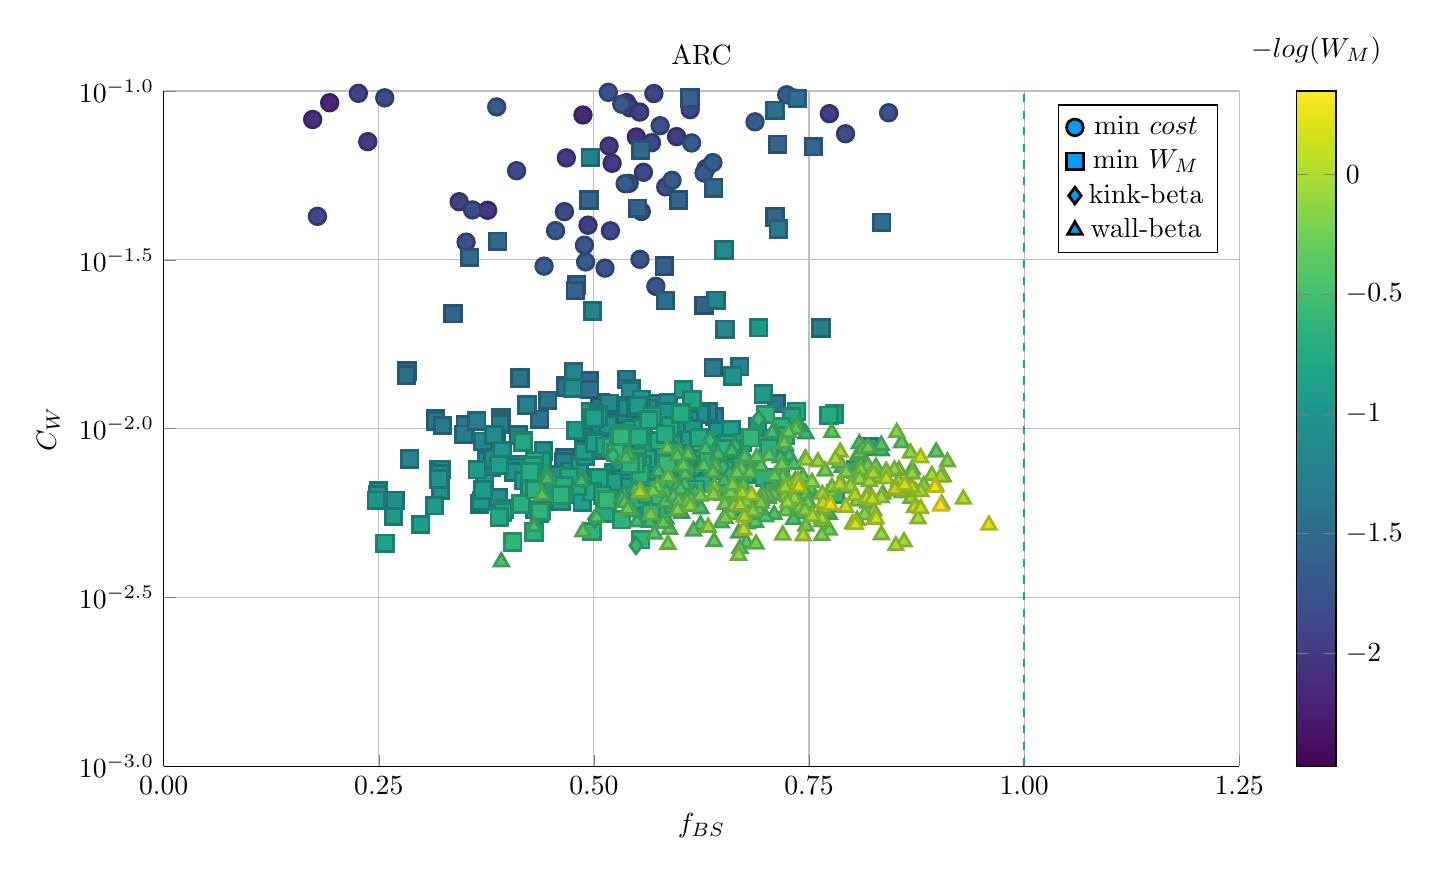
\begin{tikzpicture}[]
\begin{axis}[colorbar = {true}, height = {101.6mm}, ylabel = {${C}_{W}$}, title = {ARC}, xmin = {0.0}, xmax = {1.25}, ymax = {0.1}, ymode = {log}, xlabel = {${f}_{BS}$}, {unbounded coords=jump, scaled x ticks = false, xticklabel style={rotate = 0}, xmajorgrids = true, xtick = {0.0,0.25,0.5,0.75,1.0,1.25}, xticklabels = {0.00,0.25,0.50,0.75,1.00,1.25}, xtick align = inside, axis lines* = left, scaled y ticks = false, yticklabel style={rotate = 0}, log basis y=10, ymajorgrids = true, ytick = {0.001,0.0031622776601683794,0.01,0.03162277660168379,0.1}, yticklabels = {$10^{-3.0}$,$10^{-2.5}$,$10^{-2.0}$,$10^{-1.5}$,$10^{-1.0}$}, ytick align = inside, axis lines* = left,     xshift = 0.0mm,
    yshift = 0.0mm,
    axis background/.style={fill={rgb,1:red,1.00000000;green,1.00000000;blue,1.00000000}}
, colormap={plots}{rgb=(0.26700400,0.00487400,0.32941500), rgb=(0.27794100,0.05632400,0.38119100), rgb=(0.28291000,0.10539300,0.42690200), rgb=(0.28229000,0.14591200,0.46151000), rgb=(0.27619400,0.19007400,0.49300100), rgb=(0.26514500,0.23295600,0.51659900), rgb=(0.25042500,0.27429000,0.53310300), rgb=(0.23360300,0.31382800,0.54391400), rgb=(0.21813000,0.34743200,0.55003800), rgb=(0.20123900,0.38367000,0.55429400), rgb=(0.18555600,0.41857000,0.55675300), rgb=(0.17117600,0.45253000,0.55796500), rgb=(0.15772900,0.48593200,0.55801300), rgb=(0.14618000,0.51541300,0.55682300), rgb=(0.13374300,0.54853500,0.55354100), rgb=(0.12346300,0.58168700,0.54744500), rgb=(0.11948300,0.61481700,0.53769200), rgb=(0.12632600,0.64410700,0.52531100), rgb=(0.15014800,0.67663100,0.50658900), rgb=(0.19109000,0.70836600,0.48228400), rgb=(0.24607000,0.73891000,0.45202400), rgb=(0.31192500,0.76782200,0.41558600), rgb=(0.37777900,0.79178100,0.37793900), rgb=(0.45867400,0.81636300,0.32972700), rgb=(0.54552400,0.83803900,0.27562600), rgb=(0.63690200,0.85654200,0.21662000), rgb=(0.73088900,0.87191600,0.15602900), rgb=(0.81457600,0.88339300,0.11034700), rgb=(0.90631100,0.89485500,0.09812500), rgb=(0.99324800,0.90615700,0.14393600)}, colorbar style={title=$-log( W_M )$}}, ymin = {0.001}, width = {152.4mm}]\addplot+[scatter, scatter src=explicit, only marks = {true}, color = {rgb,1:red,0.00000000;green,0.60560316;blue,0.97868012},
draw opacity=1,
line width=0,
solid,mark = *,
mark size = 3.0,
mark options = {
    color = {rgb,1:red,0.00000000;green,0.00000000;blue,0.00000000}, draw opacity = 1.0,
    fill = {rgb,1:red,0.00000000;green,0.60560316;blue,0.97868012}, fill opacity = 1,
    line width = 1,
    rotate = 0,
    solid
}] coordinates {
(0.5241958664809654, 0.20287227770679064) [-2.471255345772589]
(0.6576174121055033, 0.2306439147061058) [-2.4448353783501813]
(0.5667366204542917, 0.21229572622839188) [-2.3420433442606363]
(0.5527453887086349, 0.17601810120802597) [-2.317452102945315]
(0.5061500178726741, 0.15646026161547585) [-2.271586680020917]
(0.2819526564955794, 0.23313397035671538) [-2.2454926622107947]
(0.5154131085826593, 0.30695982711321923) [-2.240477125239761]
(0.5121074780521085, 0.12981873154201856) [-2.221001617157497]
(0.36855232237120356, 0.20412561186382183) [-2.2185595731398573]
(0.4242321290991145, 0.17283887577812557) [-2.217742719332761]
(0.4047617309441989, 0.1723168352757067) [-2.1943652895954826]
(0.19286791326705938, 0.09228957678154598) [-2.180611452056678]
(0.5532714654641776, 0.18069474612421305) [-2.178533974810608]
(0.23145882806732, 0.17575721123179697) [-2.1613119546549586]
(0.564515028561278, 0.14737248164629663) [-2.153481889652779]
(0.2747981030966843, 0.15121971859178504) [-2.1532666027476224]
(0.4872417045079029, 0.08487876383400252) [-2.137355128792399]
(0.612166701787264, 0.18468615468864133) [-2.117721604472264]
(0.5023741300351264, 0.10225619683254578) [-2.112364994691398]
(0.17309553189891597, 0.08231272723595219) [-2.0932729799082814]
(0.8291596430779791, 0.18191471123359046) [-2.088330487139694]
(0.31718430150640886, 0.1065828154014555) [-2.0864754038765376]
(0.5273579873776012, 0.1272047508604084) [-2.0803726509713845]
(0.5595793743294597, 0.11257905190542687) [-2.0743439417542344]
(0.4605098153393489, 0.1600333280328488) [-2.060818046402037]
(0.5493219691145695, 0.07308016714475707) [-2.0557180072115067]
(0.31128212610729583, 0.12592715347430458) [-2.0556926961078257]
(0.37645603539027617, 0.044334788818868265) [-2.0190103037593397]
(0.5176809217159155, 0.06869458193202499) [-2.0160407406558845]
(0.7081188681434396, 0.1481536198793765) [-2.013932053549837]
(0.5211323398937894, 0.06108685421726483) [-2.00409352685897]
(0.5380552721473089, 0.09236557707945936) [-1.9956061889121497]
(0.23715847834480255, 0.07078434635359439) [-1.990719111417077]
(0.46795448687244745, 0.06336605700824453) [-1.9900844504935096]
(0.6557560817291185, 0.11627768440359171) [-1.9837616587056666]
(0.35068098774722584, 0.25526434794478386) [-1.9822717418460247]
(0.5960363570257688, 0.07325842242370716) [-1.9712120847707018]
(0.541926025336331, 0.08913847457348267) [-1.9636002811445543]
(0.7410857770713545, 0.15979638765383897) [-1.9571238190242108]
(0.3701358669693677, 0.20418232424592905) [-1.9546253727806209]
(0.5532971016447703, 0.08659458120814034) [-1.9463665380941702]
(0.4931141469968015, 0.040041103525576084) [-1.944009739142569]
(0.6750992151231566, 0.13342994620782112) [-1.9434041917067464]
(0.773711576159501, 0.08565629392349437) [-1.9426970317490913]
(0.34341778727051797, 0.04698977973717222) [-1.9371763921573384]
(0.40004180408095424, 0.11657734913990186) [-1.928537217281344]
(0.22621961396755902, 0.09839586000912476) [-1.9107205293107241]
(0.33982734439703416, 0.12275477488785659) [-1.9004071431399057]
(0.5696717164152757, 0.09825956480008603) [-1.8918218222163223]
(0.6089203094451604, 0.12138563536401357) [-1.8887149281050344]
(0.7855174188311217, 0.10048378866349675) [-1.8819056386780568]
(0.519165742162139, 0.03854677190172235) [-1.869430211714412]
(0.56689423388905, 0.07025107210769377) [-1.8651124798448722]
(0.17865306360793093, 0.04253804397177868) [-1.8644786123967394]
(0.6118904337598889, 0.08799392557650451) [-1.860496893823878]
(0.46571538383754973, 0.04391723622012491) [-1.8542903424441743]
(0.5575934736377758, 0.05743494936487108) [-1.8495112242429361]
(0.41012249247804866, 0.058061403117541356) [-1.846257438745883]
(0.7924354191473056, 0.07470510715125366) [-1.8416117842187498]
(0.5550986570410285, 0.04396908701659585) [-1.841317185146719]
(0.665840917415036, 0.14962201583537357) [-1.8309301799846331]
(0.6302313196317723, 0.05890018945608892) [-1.82730525270959]
(0.6638598475520857, 0.1158423978677618) [-1.826901690940231]
(0.2568814608902971, 0.09540606509282185) [-1.8239153211364227]
(0.6535189993672528, 0.12701003424511964) [-1.8168455226783244]
(0.3514379080061537, 0.03567637571358925) [-1.8166454759701696]
(0.35890190840174097, 0.0444388756442925) [-1.81017737836428]
(0.5834421319112952, 0.05199865811744338) [-1.8086978288671451]
(0.6467507601284886, 0.1251127775635393) [-1.798447628719369]
(0.7506773056708338, 0.14005152172406524) [-1.7969021740981885]
(0.5769610885682936, 0.0789099851468337) [-1.7945906278673165]
(0.5167473074126737, 0.09906247923337126) [-1.779933055929714]
(0.8424743258288371, 0.08619366633116249) [-1.7676381685595108]
(0.5128998814964993, 0.02988638548757804) [-1.7674346288089102]
(0.4890123747581225, 0.0349357030811516) [-1.748385793611066]
(0.5719886607137856, 0.026398091660566128) [-1.7474067398666728]
(0.5535801579795155, 0.0317308779482479) [-1.7473345345195481]
(0.6646042636427472, 0.13550842427034193) [-1.74675304289594]
(0.5410133779521771, 0.05327415376487706) [-1.7440444912963449]
(0.7331805458227827, 0.09528385676184899) [-1.7420641858951875]
(0.5323465099100665, 0.09137626462030565) [-1.7106233078102575]
(0.4554042355140383, 0.03859073092462427) [-1.7101957038204436]
(0.6280080521317699, 0.057157670859899604) [-1.6976377627866777]
(0.3870013471271922, 0.08970301543530995) [-1.6951046172778514]
(0.5908033630086555, 0.05437969052103555) [-1.6845366899487946]
(0.5362845083298821, 0.053158707255175616) [-1.6842882715798002]
(0.6135591627510759, 0.07015118809375721) [-1.6798255842338246]
(0.4903582554642052, 0.0311795818387021) [-1.678803886594569]
(0.7241153127543816, 0.09743173539150955) [-1.6644466872035906]
(0.44208173753609914, 0.03029149365815447) [-1.661845596221059]
(0.6382751599025954, 0.06136233850066078) [-1.6570891122908413]
(0.6872315803634489, 0.08102586935633366) [-1.6543345543312795]
};
\addlegendentry{min $cost$}
\addlegendentry{min $W_M$}
\addlegendentry{kink-beta}
\addlegendentry{wall-beta}
\addplot+[scatter, scatter src=explicit, only marks = {true}, color = {rgb,1:red,0.00000000;green,0.60560316;blue,0.97868012},
draw opacity=1,
line width=0,
solid,mark = square*,
mark size = 3.0,
mark options = {
    color = {rgb,1:red,0.00000000;green,0.00000000;blue,0.00000000}, draw opacity = 1.0,
    fill = {rgb,1:red,0.00000000;green,0.60560316;blue,0.97868012}, fill opacity = 1,
    line width = 1,
    rotate = 0,
    solid
}] coordinates {
(0.5817114877806479, 0.03030964076750237) [-1.6347176951799236]
(0.6118616823524671, 0.09519865042001042) [-1.6073278771107937]
(0.550825513446965, 0.04494796053659054) [-1.584364281605552]
(0.47990293428614395, 0.026650965215041525) [-1.5820971810203286]
(0.6280353944665124, 0.023183384776903366) [-1.581333652067033]
(0.49437603226420324, 0.047519264379099695) [-1.5776358054595747]
(0.3362571361359799, 0.021900164864569343) [-1.5739276291567563]
(0.5982172603264796, 0.04756226129621259) [-1.572108505738868]
(0.7135274551952335, 0.06954867549545035) [-1.5672962391673115]
(0.47833927674197335, 0.02566305684475041) [-1.5665040064849882]
(0.7103341191962936, 0.04235079729891905) [-1.5555149127719143]
(0.5543093285365798, 0.06695317015759708) [-1.543581310599075]
(0.7551306424351277, 0.06841478633789891) [-1.5260699424888133]
(0.3881783683118415, 0.03590196542626109) [-1.524227611937092]
(0.6393151095771953, 0.05163649629310236) [-1.5216893138751995]
(0.355597836411217, 0.032143280375917176) [-1.5039859914912947]
(0.4945318173106939, 0.013866958448834382) [-1.493326092363065]
(0.28281884884932085, 0.014801741304267257) [-1.487901247382047]
(0.28211632020593413, 0.014412667219330384) [-1.4777729839057352]
(0.7104365991482212, 0.08761412553231249) [-1.4621624345903141]
(0.7363692362152062, 0.09498385047870876) [-1.4604586034356677]
(0.8344486043341511, 0.04081913693413996) [-1.4587214825346047]
(0.46708133454393946, 0.01340972738128021) [-1.4490727286546803]
(0.5831555839731757, 0.023945948554713548) [-1.4457290774204032]
(0.5075718306406568, 0.011911642809951824) [-1.4426440160762033]
(0.46706461267458904, 0.013297745600298047) [-1.4402960124898458]
(0.4950737862291223, 0.013059974842794808) [-1.4297123303293562]
(0.5067238822314855, 0.0116292993719446) [-1.4185999884517813]
(0.44619912372103193, 0.012144168284609194) [-1.4088672496121717]
(0.31605802663087745, 0.010680636478422217) [-1.3865730777653493]
(0.41428673202754596, 0.0141353915084305) [-1.3853300727274243]
(0.712239885615206, 0.011858386666639936) [-1.3837167890494473]
(0.350431541268587, 0.01028527278110118) [-1.3831077459191452]
(0.43685814056517275, 0.010657247043679216) [-1.3769740136231394]
(0.3159315431374323, 0.010544710114440428) [-1.3745163187278553]
(0.5413118800861578, 0.01102120660236595) [-1.3615967553395791]
(0.7142435030748111, 0.039062963614451315) [-1.3533380016716623]
(0.3240459840226499, 0.010216036443098337) [-1.3372087645633441]
(0.3920447348241641, 0.010766373691067175) [-1.3345129020147544]
(0.6388083334581369, 0.01515074267205838) [-1.3192755308000974]
(0.39164878205902165, 0.010549186267561154) [-1.314224057600752]
(0.3488127094714696, 0.009622849310238562) [-1.3119655997760449]
(0.5378910611821822, 0.014012905880008366) [-1.3067859154211212]
(0.7641042278711495, 0.01987362470678978) [-1.306488109771051]
(0.36380256670479283, 0.010543596556449621) [-1.300448172019359]
(0.42213038169068423, 0.011753733588622684) [-1.2909613135050368]
(0.39123076658058537, 0.01032210691217398) [-1.290941195447848]
(0.412247493693321, 0.009573931433783737) [-1.288382478225186]
(0.4659585061159808, 0.008214078605189646) [-1.2848508011023854]
(0.38667992917631405, 0.009313214534419275) [-1.2663273942574376]
(0.6399920560778708, 0.010859939566305288) [-1.2628532071739471]
(0.4932184016134092, 0.00942852126782232) [-1.2571675985941009]
(0.4646455314624805, 0.007979384853642458) [-1.2548029920250783]
(0.3808496705423307, 0.007684943962399527) [-1.2437033135541056]
(0.4958659013831641, 0.06352567671838111) [-1.2369052187227225]
(0.5000213263897932, 0.009002465988456979) [-1.2270518720108157]
(0.5308438797997663, 0.011035208951789109) [-1.226245033465833]
(0.6694205694501582, 0.015249972586931702) [-1.2235700920501882]
(0.5693740544983247, 0.00868692401548569) [-1.2226473193604595]
(0.6417688448023928, 0.023992084814044464) [-1.2216425458700924]
(0.5487244266906349, 0.008820048824892238) [-1.2211984240451863]
(0.2858601406466925, 0.008128091853447697) [-1.2182589804749475]
(0.5156304286810139, 0.009127494309245325) [-1.2142161347607898]
(0.47639998325402977, 0.014715113037040341) [-1.2132136425529505]
(0.5288813993673583, 0.010793413620685892) [-1.206641818571807]
(0.5402250120741555, 0.009362601672990878) [-1.191936852103939]
(0.5727465096226879, 0.008532248708843341) [-1.1915692690246116]
(0.4984364208598661, 0.022329699785653967) [-1.1862171477514327]
(0.6327644843335064, 0.011220902449602043) [-1.1850949532660688]
(0.5065941888585173, 0.009964976977277301) [-1.1849042685186388]
(0.3751135189163956, 0.008046818607636182) [-1.1783816195421168]
(0.5288430725634312, 0.010502630239530353) [-1.1745570808178625]
(0.5743220494611327, 0.011831696332363917) [-1.1739049960816583]
(0.49014706797846697, 0.008338714638816998) [-1.1727262972250005]
(0.5428976258536967, 0.013100649505701023) [-1.1685715861060364]
(0.4876473654064088, 0.008679297866717622) [-1.1678361124508785]
(0.37098217471657124, 0.009176059619375874) [-1.1638475083020863]
(0.6512553694339193, 0.009147667338886346) [-1.163646396682439]
(0.5119225508554565, 0.008821522947817238) [-1.1625884970295683]
(0.6522013945133583, 0.01969269746480885) [-1.161263163747147]
(0.5367974717464423, 0.011052820822833412) [-1.1612436952445022]
(0.5422654663131025, 0.012951176392377263) [-1.1564975464369418]
(0.5110846173942302, 0.00865659180620948) [-1.1564777605259131]
(0.5353295518280365, 0.008539920889371473) [-1.153669555256764]
(0.5173196862178037, 0.011881223263670228) [-1.1449033146577834]
(0.6129510277633284, 0.011182674502441104) [-1.1446379399297224]
(0.3201525037042981, 0.00758528934201417) [-1.1369019245716605]
(0.642193788855941, 0.009173443590563553) [-1.1296752949778874]
(0.5535992683176709, 0.008338540154559412) [-1.1286199217371102]
(0.6513872112772378, 0.03379772419568562) [-1.1227901581286868]
(0.5384174946071185, 0.011716658365690755) [-1.1213706798498402]
(0.44262055397654837, 0.006600498288231924) [-1.120744758255219]
(0.38214281120318244, 0.008128082189126142) [-1.1202374603300567]
(0.4722194839752176, 0.007485071081146149) [-1.1198130519550673]
(0.3228255089630173, 0.00757188435534942) [-1.1197010006946204]
(0.38371417796295587, 0.0095811845612121) [-1.1171509659015317]
(0.624252275623572, 0.011241415941032132) [-1.1142292859317902]
(0.5355455264892967, 0.009608134033428447) [-1.111737343141002]
(0.5727668427351763, 0.01112408759755598) [-1.109744376511266]
(0.4114801256653036, 0.007847073705149175) [-1.1077966249084845]
(0.5382787031018355, 0.011559534016906275) [-1.1071823666105103]
(0.31965994829173516, 0.0073510161641234155) [-1.104798498774279]
(0.5384075099986052, 0.007531141843880735) [-1.1010716645822378]
(0.5864126224331899, 0.011959627018568285) [-1.1002751733513731]
(0.557617660880907, 0.007903291194171595) [-1.100001261719793]
(0.47549886995354823, 0.013186084887405795) [-1.0994225265487236]
(0.623037942078233, 0.011066567940261007) [-1.0985618635225085]
(0.5033268621050487, 0.00915283698682942) [-1.0949280603220852]
(0.2688518460791765, 0.006133703525212153) [-1.0934361516365225]
(0.6110478224857046, 0.010640115882783727) [-1.0929493330528903]
(0.558520760663903, 0.008947359142857395) [-1.0928608320296447]
(0.32155511158393607, 0.0073486051811523) [-1.087706069497112]
(0.4758264456361486, 0.006376305301764062) [-1.0862007240731857]
(0.4097926766511398, 0.007683528007593692) [-1.0852670263146056]
(0.5502315352756275, 0.008000466946774797) [-1.0851636190972072]
(0.5566953268770855, 0.0076693437218355535) [-1.0840894132396022]
(0.3216722475930553, 0.006579330015555362) [-1.0835229356564555]
(0.45567205862575944, 0.007297986251593657) [-1.082817350704825]
(0.36696671117349405, 0.005986051223044731) [-1.0820717451803519]
(0.3891852359575543, 0.006234773177915995) [-1.072577404791479]
(0.24971176414080096, 0.00656095951928795) [-1.0722121269518887]
(0.5633918208276852, 0.011424148754591202) [-1.0713713808748146]
(0.6042975616419993, 0.01019215515273024) [-1.0693614816162402]
(0.5485022627546088, 0.011520946380794598) [-1.0668579057002654]
(0.5553825174671281, 0.008690353228069395) [-1.0614717160120588]
(0.6436681416631705, 0.009857214240237989) [-1.0539224257593203]
(0.5231064369976265, 0.007410533138876833) [-1.0510937327305279]
(0.4070604216031404, 0.007449838707835127) [-1.0497007973704187]
(0.3198885646073333, 0.007088919319303044) [-1.0471558619826447]
(0.4414420283273741, 0.008599918404779687) [-1.0461189694088024]
(0.24867057556472014, 0.006377309887140109) [-1.0418966319978196]
(0.6376541673006868, 0.0075647796759351965) [-1.038421761130219]
(0.6009251138878389, 0.009882058577592544) [-1.036521934372695]
(0.41776764665149635, 0.009223959289867847) [-1.0356215569640665]
(0.5842492103852158, 0.011206142984745959) [-1.032265172493932]
(0.5159535753171318, 0.010275809470086928) [-1.0209529420786516]
(0.4959672719731226, 0.006909070463416791) [-1.017778295850808]
(0.661391258299459, 0.014318337912922812) [-1.0164185835880817]
(0.5608498014090172, 0.010831709750721097) [-1.0158514857486804]
(0.6151725048676855, 0.009969004456469335) [-1.0092640911327964]
(0.5314443614911326, 0.0076830709125841655) [-1.0065489183190215]
(0.5286944439645233, 0.007109903886026088) [-1.0049567352420634]
(0.5552755893210628, 0.012210250424143995) [-1.0009019288888164]
(0.5581675745958038, 0.007769954338030814) [-1.0006461053349212]
(0.24716026898994242, 0.00614165224338566) [-0.9994054785850832]
(0.504350487641437, 0.006788464214574843) [-0.9973161692403991]
(0.3934424737113256, 0.008588102458327246) [-0.9969035241117329]
(0.4796243766218075, 0.006868288351132624) [-0.9965363238277729]
(0.52700034066082, 0.0068423979356222785) [-0.9922669644795622]
(0.37317354020546645, 0.006930487452016415) [-0.9885003181225582]
(0.6089875710029672, 0.008132058870519111) [-0.9840022040037167]
(0.4213909625587017, 0.007028212307439231) [-0.9804048117014232]
(0.4833180602931159, 0.007774353597955766) [-0.979522354913071]
(0.26710604767533075, 0.0054956368744154315) [-0.9765348801577157]
(0.42944101394074274, 0.007267240459298835) [-0.9755629318997818]
(0.3691943435583234, 0.0061040685529331245) [-0.9749892927335156]
(0.49008340947678686, 0.008312108043668191) [-0.9674264957309127]
(0.43100817708896116, 0.005754155204131383) [-0.966984586559087]
(0.3146511741196146, 0.005916229247218672) [-0.963620689023264]
(0.6915196643186565, 0.019907252097557806) [-0.9635570646594878]
(0.6969186730398873, 0.012656834856123324) [-0.9589381201418358]
(0.5343246872696013, 0.006890734339357853) [-0.9584027445972434]
(0.5516547055046426, 0.01170966388492377) [-0.9563855192144691]
(0.45055913702267586, 0.00648495859205545) [-0.9554467273670927]
(0.36443125720312075, 0.0075610875798886755) [-0.9545632580533228]
(0.6903219512667356, 0.010114178702367332) [-0.9528002583069045]
(0.592139488874089, 0.009004872969664781) [-0.9496533928753537]
(0.49580893715304947, 0.011207230671626593) [-0.9413852860902241]
(0.6235670164997241, 0.007146213704940033) [-0.9370119952675158]
(0.37108589969685146, 0.006581879826789411) [-0.9331828097449962]
(0.6437665262857747, 0.008767448947945771) [-0.9329352040317512]
(0.4888947150611439, 0.008557021700551098) [-0.9324303568969876]
(0.2986086480277226, 0.005203512160232155) [-0.9311662336138826]
(0.6255293508491894, 0.008081114013096696) [-0.9287944685604638]
(0.6140870094258984, 0.007628598443188674) [-0.926890870969113]
(0.41876798527701836, 0.007018485606889323) [-0.92386498939783]
(0.5054852519528996, 0.011015711855547592) [-0.919580931517054]
(0.4786536293159207, 0.009893013391436023) [-0.9180169825194476]
(0.5441671870525477, 0.009982337828276887) [-0.9154453649397588]
(0.5007878466101845, 0.0091944581117192) [-0.9139490923741643]
(0.561487282467392, 0.007833072636536566) [-0.9132133538239265]
(0.6514919308345418, 0.008840033410607953) [-0.9121378643433682]
(0.6039078741957786, 0.013068265001934793) [-0.9110784645494641]
(0.6227409498560608, 0.007938450262022891) [-0.9098658111730449]
(0.6435481039076728, 0.008553630272950136) [-0.9070051498915257]
(0.6010749539644062, 0.007575552407024117) [-0.9067782074518957]
(0.5348620647926116, 0.006729621026089755) [-0.9060762300599821]
(0.8195604933647264, 0.008858181214516578) [-0.9039670080592699]
(0.4960911849247666, 0.010768315647388733) [-0.9014867608639769]
(0.5049187404089968, 0.010808877533630424) [-0.9007952929826429]
(0.5008305537160933, 0.009078214918907012) [-0.9007062506970809]
(0.5137960656889574, 0.007073305102824147) [-0.900208401387847]
(0.4299758063065358, 0.007716380916945232) [-0.8984405159461796]
(0.461950405654823, 0.006106767180219444) [-0.8982477432771846]
(0.6509355541893169, 0.008695264992095957) [-0.896003666359785]
(0.5225903676252684, 0.006941829479120447) [-0.8955056224321819]
(0.3894845570414093, 0.007814299518066377) [-0.8942100046557695]
(0.4394904947732839, 0.008028972189491295) [-0.8890699913254794]
(0.5003005570537615, 0.010728044838137048) [-0.8876712498055658]
(0.5845386590677969, 0.008310610689471132) [-0.8863260728535448]
(0.6591714169241578, 0.00991040208694835) [-0.8837201982810288]
(0.5754886167651249, 0.00719216253641406) [-0.8834009298105716]
(0.42859653650833, 0.007585939375582381) [-0.8806916777259077]
(0.6118081005357805, 0.009272863725182066) [-0.8796719383127752]
(0.48641611954822667, 0.006055492371240138) [-0.8726396490009896]
(0.257229546671479, 0.004580349740413994) [-0.8672923383997936]
(0.426462607268772, 0.007407120757886044) [-0.8535433362712267]
(0.5686669963907276, 0.008621646255895433) [-0.8533325571574846]
(0.6175106036050393, 0.006609354191499301) [-0.853129954975184]
(0.5877104639523651, 0.008626640245331227) [-0.8458427202328871]
(0.5716419045548307, 0.007926356626055567) [-0.8399949391566971]
(0.3962776710982887, 0.005783758781719592) [-0.8344337866440044]
(0.4255334400440256, 0.006679285642911387) [-0.8328143677232719]
(0.43857941286956165, 0.005735056256784172) [-0.8320308752066863]
(0.5769445652964436, 0.007843029441706253) [-0.8221569652352421]
(0.6611817268556156, 0.008093343165007398) [-0.8172218943340012]
(0.5126668648272711, 0.008863355456490663) [-0.8131136245599477]
(0.3941080030492619, 0.005668771371327368) [-0.8122740065328773]
(0.506119518337849, 0.007155161987838886) [-0.8080036926936133]
(0.6141107199137688, 0.008031459191263671) [-0.8071539542338575]
(0.6139955223319464, 0.012167930923139617) [-0.8069124707651293]
(0.6417146223223801, 0.008948962637139601) [-0.8052829756994823]
(0.5669733040046213, 0.006679423174117699) [-0.8020427686638395]
(0.7356948340040768, 0.011264900432107284) [-0.8005903298305235]
(0.5882544255345495, 0.0101736730249019) [-0.7977331662395057]
(0.6728655549820258, 0.009118819889961022) [-0.7969461494732382]
(0.5679841220109311, 0.01094150991845671) [-0.7969287961306641]
(0.6222675762661165, 0.009204618947872185) [-0.7946481033628194]
(0.4310732454261373, 0.008047254921185912) [-0.7926515245490977]
(0.4177825334190035, 0.009132260578460593) [-0.7893816917258589]
(0.4369556767367021, 0.005606722466908005) [-0.7891633883074732]
(0.4977504961312478, 0.006506117273958602) [-0.7806626165140812]
(0.5618987698011563, 0.008151671842735457) [-0.7792790884221499]
(0.556998592933926, 0.010062331825114089) [-0.7784524078397926]
(0.6554923199603303, 0.009001558635684543) [-0.7779808320754125]
(0.39004777043616934, 0.0054810011900626385) [-0.7720609309973395]
(0.5562151504078756, 0.00782695612444411) [-0.7652054854871606]
(0.5635456677693395, 0.010602248839245204) [-0.7637174087569671]
(0.7298248277431699, 0.010869712908743537) [-0.763435051327913]
(0.5099920259552589, 0.006363325083353543) [-0.7618517639809802]
(0.7795217235236127, 0.01105835991924475) [-0.7614993450910051]
(0.5128038581202035, 0.005635574040670621) [-0.7611032574956281]
(0.5843531099526409, 0.007945573763413242) [-0.7586493247490348]
(0.6783775994948534, 0.00746361599356464) [-0.7555286255013439]
(0.4287240355308217, 0.0077689317654998065) [-0.7546589867802752]
(0.615129822924657, 0.008443992254390653) [-0.7545235423813055]
(0.6198452199457032, 0.008351019459044646) [-0.7530552699688687]
(0.575573732558629, 0.009207860738462068) [-0.7525689023877592]
(0.6510139446420534, 0.0076258608035912135) [-0.750871938891472]
(0.6224512800040214, 0.009388924409384974) [-0.750814319098593]
(0.6012103864677005, 0.01118644198035734) [-0.748723305421913]
(0.7069020464705562, 0.009345849525045828) [-0.7483206071488305]
(0.4805514422966483, 0.006768249757897973) [-0.7464367414626797]
(0.4708373767438117, 0.007223518482823314) [-0.7461140334995429]
(0.7731485889984414, 0.010949849394014196) [-0.7445921563372909]
(0.8037621486342045, 0.0075644226280255) [-0.7405170531585982]
(0.6757344825134481, 0.007343719666417131) [-0.7390004613202035]
(0.6594328314470048, 0.008700856720017821) [-0.7387616236204831]
(0.626762429902987, 0.00688316527472499) [-0.7380863769707697]
(0.5829650043598863, 0.00962175642804203) [-0.7368937154713704]
(0.6007965815988566, 0.011034885333216478) [-0.7342730225098203]
(0.5580883743814108, 0.006379564580150208) [-0.733902575813519]
(0.5441864591828873, 0.005838014810087431) [-0.733366320896288]
(0.570430479648329, 0.005798113597019041) [-0.7194953671868318]
(0.4653459017068548, 0.006758912533271294) [-0.7147746128167595]
(0.5523041252103958, 0.009475051889139297) [-0.7131077088888362]
(0.41526223236330206, 0.005978841286873692) [-0.7060108538400767]
(0.42552016721166286, 0.007437940638478416) [-0.7054470522681139]
(0.6239617621329132, 0.008396523209957296) [-0.7043302537280044]
(0.6279845069667198, 0.008135075629052014) [-0.7004921579289034]
(0.5881492261240776, 0.006868958471786255) [-0.7001780528099326]
(0.5506350458775752, 0.00825632250348302) [-0.6977184423457128]
(0.6979968249478757, 0.007177220657115959) [-0.6956779138722414]
(0.6568303568061684, 0.007022224715140027) [-0.6951251649106842]
(0.6182818991073687, 0.006613282053180216) [-0.6924358169248216]
(0.5510239579883293, 0.0061493207913365135) [-0.6909665152137748]
(0.5702234268112552, 0.006107066134008809) [-0.6835279600057703]
(0.703320903908008, 0.008780796565424387) [-0.6827611083117922]
(0.7077673334600145, 0.0065261506973616846) [-0.6795072230761997]
(0.5495829548416775, 0.00800959338461906) [-0.677700463862544]
(0.4314935730470368, 0.006600686007871915) [-0.6763055623723756]
(0.43054195576046844, 0.004950028138324652) [-0.6703030174757271]
(0.5635130294426022, 0.005539486392576543) [-0.6677810778235018]
(0.553595959152619, 0.007362527200082348) [-0.6673391087292244]
(0.6519599706166325, 0.008739904111948478) [-0.6667743364683484]
(0.5824517878555476, 0.006646109301375384) [-0.6628604680937062]
(0.7176408995573551, 0.010112687007456347) [-0.6619264755699156]
(0.5770682825422682, 0.005808955328171345) [-0.6609430387636127]
(0.6024550183113115, 0.006226486976685874) [-0.6608237273970524]
(0.5478348614019433, 0.007880168654276763) [-0.6591974827031457]
(0.5208453986930105, 0.00880835203629707) [-0.6555251605106848]
(0.5959294410528901, 0.0069051641790013815) [-0.6502439759277362]
(0.46157053437184653, 0.006370154893781598) [-0.6501176336530103]
(0.716721708615555, 0.007046016170190783) [-0.6471624229162491]
(0.5422497797368149, 0.00786400613866977) [-0.642689222490187]
(0.676581400539928, 0.006126476505793275) [-0.6426719680934136]
(0.43755139645655033, 0.00568605172293329) [-0.6421657799692642]
(0.5322226344638359, 0.005380439014465079) [-0.6408278053086536]
(0.6315922459562998, 0.008151332535041496) [-0.6390518480231551]
(0.5289646632563154, 0.009445426881617458) [-0.637387036100165]
(0.5629402113776424, 0.006410449458406456) [-0.6331856765913819]
(0.6064256092688981, 0.007534711658278645) [-0.6317878364268024]
(0.699534914937192, 0.011020608245919671) [-0.6302067113060754]
(0.7227329826277413, 0.009531906181488446) [-0.6300141158962402]
(0.5326012265639793, 0.009634058044917598) [-0.6280804941242557]
(0.6330084093380534, 0.008014239654104959) [-0.6280494211696446]
(0.6507439971206197, 0.007547331772442004) [-0.6280078234260247]
(0.40558390299155495, 0.004613850780468482) [-0.6272747005855834]
(0.7806276684554971, 0.006403443257132637) [-0.6249924315441349]
(0.5542724771727453, 0.004688384323580258) [-0.6203497363094942]
(0.7379632139747722, 0.00673286293260975) [-0.6186335699037506]
(0.6491547712439395, 0.006536718541121758) [-0.616611980354735]
(0.4976979810985317, 0.004961181636973083) [-0.6158983852690758]
(0.5922925103137072, 0.005978684032577509) [-0.6126591649688387]
(0.6603227030387234, 0.005906726926903094) [-0.6115944493416251]
(0.5316308102551144, 0.00947881794063107) [-0.610433329147383]
(0.6827036729203786, 0.009411403397962845) [-0.6100633867421124]
(0.587302343499971, 0.006804926481153247) [-0.6086993044360022]
(0.576987349595759, 0.006194075724438983) [-0.5997038129358795]
(0.5849100380517773, 0.007840734610599833) [-0.5989923200136442]
(0.5667143656682501, 0.005628681372057809) [-0.596937261397637]
(0.525146575549925, 0.008492276760383373) [-0.5958587738741902]
(0.515389531675495, 0.006157094838169622) [-0.5927256123541282]
};
\addlegendentry{min $cost$}
\addlegendentry{min $W_M$}
\addlegendentry{kink-beta}
\addlegendentry{wall-beta}
\addplot+[scatter, scatter src=explicit, only marks = {true}, color = {rgb,1:red,0.00000000;green,0.60560316;blue,0.97868012},
draw opacity=1,
line width=0,
solid,mark = diamond*,
mark size = 3.0,
mark options = {
    color = {rgb,1:red,0.00000000;green,0.00000000;blue,0.00000000}, draw opacity = 1.0,
    fill = {rgb,1:red,0.00000000;green,0.60560316;blue,0.97868012}, fill opacity = 1,
    line width = 1,
    rotate = 0,
    solid
}] coordinates {
(0.6426659794233436, 0.00815561907827368) [-0.5919909182692854]
(0.5467348022827744, 0.006659517069337427) [-0.5900649293210665]
(0.7190311064983813, 0.007508093393788605) [-0.5846116951906657]
(0.6111339025872151, 0.007527132152211165) [-0.5833148125881625]
(0.6497883761170222, 0.007696247444472184) [-0.5830287350896988]
(0.6912674151371413, 0.010658010749014063) [-0.5820887710705529]
(0.5010169539514072, 0.005401882204713616) [-0.5820189989610497]
(0.535207082269819, 0.006378967305214437) [-0.5810074819933287]
(0.738016225952711, 0.010217682877138867) [-0.580249699669254]
(0.6642282356732003, 0.008850762543020996) [-0.5794750614001255]
(0.7241697567719548, 0.008618003799358996) [-0.5792296887118283]
(0.6755643086904745, 0.007360374433648833) [-0.5788547078152965]
(0.5490007479996606, 0.004512048645314757) [-0.57645307994183]
(0.7689819041990633, 0.006116989896278519) [-0.5763924759645073]
(0.5220335653648919, 0.008318627601371252) [-0.5729750222272765]
(0.4868290703396239, 0.007101945083232647) [-0.571357101904463]
(0.8201613481545499, 0.0074318775027898635) [-0.5687383147863687]
(0.6349821386738914, 0.00921889738378825) [-0.5664495516615029]
};
\addlegendentry{min $cost$}
\addlegendentry{min $W_M$}
\addlegendentry{kink-beta}
\addlegendentry{wall-beta}
\addplot+[scatter, scatter src=explicit, only marks = {true}, color = {rgb,1:red,0.00000000;green,0.60560316;blue,0.97868012},
draw opacity=1,
line width=0,
solid,mark = triangle*,
mark size = 3.0,
mark options = {
    color = {rgb,1:red,0.00000000;green,0.00000000;blue,0.00000000}, draw opacity = 1.0,
    fill = {rgb,1:red,0.00000000;green,0.60560316;blue,0.97868012}, fill opacity = 1,
    line width = 1,
    rotate = 0,
    solid
}] coordinates {
(0.7462328069126333, 0.009658524804105862) [-0.5601806209906858]
(0.733172140132461, 0.009987089667958969) [-0.5562142102431887]
(0.5325765388928654, 0.006226980540213371) [-0.5546880975085333]
(0.48540116680452616, 0.006988389031410877) [-0.5546446379212883]
(0.7213776765994893, 0.008732199148890674) [-0.5527698445398843]
(0.5646666533871787, 0.0052782873859023235) [-0.5511724233466424]
(0.6714883414104902, 0.006758297452000886) [-0.5458972121667514]
(0.6601590663603173, 0.008578141254814193) [-0.5458860807447207]
(0.61755852581437, 0.006467365285710576) [-0.5458790392173498]
(0.6069869283782695, 0.006443372817331658) [-0.5442175823270508]
(0.5750781331317051, 0.007444861036885179) [-0.5413629376616981]
(0.727120523648623, 0.008302826464105732) [-0.5407622305316014]
(0.8128499975149293, 0.007384818258648993) [-0.5380836133571618]
(0.4306345366490387, 0.0051300400638977835) [-0.5271444131838583]
(0.8339385882595673, 0.008602828358081035) [-0.5255090614858061]
(0.5500607622948984, 0.005298542813562824) [-0.5253112111160531]
(0.7164670912246649, 0.00819333918907477) [-0.5250086452090449]
(0.5474078932391263, 0.006599322440552919) [-0.5242581607842178]
(0.4452999137040005, 0.007353208884415579) [-0.5231634782341672]
(0.7094608911319944, 0.009826071077992524) [-0.5227222290441186]
(0.6704331503746649, 0.007775498450419187) [-0.5219300178618078]
(0.6444318946293824, 0.008375722675050382) [-0.5198234212377003]
(0.7146410804813309, 0.007439576027519643) [-0.5189423618344886]
(0.8072587227386677, 0.007085938022585789) [-0.5186559955617387]
(0.6515622757906024, 0.006989705805817807) [-0.5166768825560152]
(0.5836822932756094, 0.005403589710063612) [-0.5164750444191784]
(0.6780755069604057, 0.00522792590340526) [-0.5150980193064546]
(0.7071972425081949, 0.009714078296726672) [-0.5116011475894415]
(0.679146758206047, 0.008045443940040638) [-0.5108110236477874]
(0.6808115221769371, 0.006168650038348271) [-0.5086504350341889]
(0.7374570975653366, 0.010169283525689762) [-0.5058613464182684]
(0.8044487812948686, 0.007149224983922412) [-0.5044722675881411]
(0.6296116692519093, 0.008692377887529698) [-0.5031231924360503]
(0.44561234746837186, 0.007078098376377251) [-0.5028014569802962]
(0.7371135032871843, 0.005600084111327829) [-0.49869154414562766]
(0.6021442829696081, 0.0056125112484924035) [-0.4964599787823767]
(0.7378562224611037, 0.006989055802710069) [-0.4945330849408947]
(0.6013683340726933, 0.007748863368021302) [-0.49445009887788993]
(0.7119963782427297, 0.006902280893600737) [-0.49421586588303207]
(0.5455023731513893, 0.00566014678548545) [-0.4927895263450095]
(0.7255648759242043, 0.006279314886066035) [-0.49104432776578616]
(0.60544395537041, 0.0068196328329766425) [-0.4894491120094672]
(0.7255010248872851, 0.00586645675685587) [-0.4893731598482633]
(0.5961553356023347, 0.006713212862122576) [-0.48832643657065083]
(0.5405651809371826, 0.008344152391720813) [-0.4837586148470547]
(0.6244169439986023, 0.005795513687709428) [-0.4825057004434148]
(0.6699821798782176, 0.006822419925958226) [-0.4783695632105468]
(0.7884090567905805, 0.0076750515586257026) [-0.4778398107696417]
(0.7519821815458965, 0.006526727405836678) [-0.47615589494341126]
(0.606748467416823, 0.006076553561977724) [-0.4730246070917381]
(0.392373899848176, 0.004034790840437016) [-0.470381466184941]
(0.5844565869358972, 0.006479697957912273) [-0.46993988320225344]
(0.5374613782498835, 0.008165717336542033) [-0.4599766548042699]
(0.7321744577656044, 0.00538496287190979) [-0.45679107520810514]
(0.7323003853039213, 0.007848284231912143) [-0.4556219511821275]
(0.6005621660529309, 0.006600712155717754) [-0.4541668738184995]
(0.5031187110819957, 0.005454374636268768) [-0.4541064555241812]
(0.6126170800310774, 0.006125431816143641) [-0.4482955765676848]
(0.668355629932245, 0.0049059331399938155) [-0.44330924134877586]
(0.5946405329652326, 0.0056884836810024665) [-0.4427268704486458]
(0.606127810669948, 0.00731015290010166) [-0.44041188876301346]
(0.5990118160542135, 0.008551905531982902) [-0.4365732513919964]
(0.7456229467861399, 0.006367061568570841) [-0.43442596765666475]
(0.7202208309321447, 0.006761746354812581) [-0.43387758013866323]
(0.70952783567679, 0.005563916117757399) [-0.4286538673039319]
(0.699400290911475, 0.005480365884552941) [-0.4276593825982841]
(0.7393643087306998, 0.0062328465646338095) [-0.42677922558914155]
(0.6754629940735157, 0.00823395238579714) [-0.4265845359620904]
(0.7735702723950867, 0.005576683303865097) [-0.4263068075286862]
(0.6409170657777765, 0.007743741682150177) [-0.4248706605294772]
(0.5355224195610914, 0.0060366402560654946) [-0.42413966208895976]
(0.6479845635204572, 0.005263353300940577) [-0.4238953032901039]
(0.8085801490222563, 0.009024229969660702) [-0.4219301249136499]
(0.7118120504162843, 0.006671380181833438) [-0.4212383781626998]
(0.6595230555223146, 0.006486848222760267) [-0.4211778292210473]
(0.7756989961427158, 0.005863656687390416) [-0.42083484997410747]
(0.6239423318389465, 0.0051872913966039755) [-0.4176858743982254]
(0.8340073111971985, 0.008923153267776813) [-0.4125562162366198]
(0.751253706001916, 0.006633187100771731) [-0.41169860837029726]
(0.6131944579781969, 0.006189362812918045) [-0.4099354279936363]
(0.6093952446214297, 0.0083818741421803) [-0.4085744725915447]
(0.5826706652528132, 0.006049286496410891) [-0.4069630403485362]
(0.5968306925560191, 0.008297436412824197) [-0.4049846840705445]
(0.6937388488296713, 0.007742960768709124) [-0.4042004215441917]
(0.807827302186393, 0.007710669480181297) [-0.40320375837586364]
(0.7493153652493619, 0.006046061667925805) [-0.4028688677214397]
(0.5704013306287763, 0.004876529539216102) [-0.40001632289493805]
(0.5926248386168477, 0.006291433392085979) [-0.39976440163800875]
(0.7457396490099157, 0.008125237867570167) [-0.39804950655742244]
(0.6735584244562056, 0.006832906261032673) [-0.3970770857727276]
(0.7113953447902368, 0.006432248216156749) [-0.3908177018779014]
(0.7339871047747247, 0.007013862412780068) [-0.38805955987639323]
(0.7898500761552186, 0.006674804159855323) [-0.3864584691344222]
(0.6415707821544318, 0.006515832091950333) [-0.38429551664195744]
(0.6773994051537632, 0.004594344989791947) [-0.38405297410594313]
(0.6909900491216344, 0.005763218077573875) [-0.3831646466050567]
(0.6878883276184834, 0.005276300390961798) [-0.38294236861775216]
(0.7696564625783999, 0.005655464618579456) [-0.38288131062137803]
(0.43972942177297236, 0.006343046844021776) [-0.3823751133382093]
(0.6279411180967263, 0.00773200722515927) [-0.38146928666653984]
(0.8066328176721882, 0.008319222350851295) [-0.3795965309572695]
(0.5880353468087063, 0.005035636185664139) [-0.3740567262619664]
(0.6384363974416298, 0.0074073940583266225) [-0.37299740292253786]
(0.7464667473070459, 0.006389790707824904) [-0.3718977586029718]
(0.6158214440985598, 0.004979442746730671) [-0.3704439735448674]
(0.7214914188453198, 0.007296148641962362) [-0.3699388031456463]
(0.7088888557638892, 0.0065537429344493196) [-0.3673465484223324]
(0.7088839124292632, 0.006366328648950684) [-0.3663620347324109]
(0.554740742245829, 0.0065777201335919366) [-0.36473337871738076]
(0.7036680845446371, 0.008314725163938977) [-0.3621711889526386]
(0.8081121115464637, 0.008453236325245295) [-0.3621650615964567]
(0.7347906764983646, 0.009973310900945706) [-0.36211407373184695]
(0.785627176052173, 0.007908310098930752) [-0.358208177595687]
(0.85769284659742, 0.009085903374204375) [-0.3540595481577626]
(0.7292127935645752, 0.006346372007983234) [-0.353783118987174]
(0.7025239274779016, 0.0062192322127949005) [-0.35222463984026725]
(0.6904176389091119, 0.006037846604665242) [-0.3509025316268699]
(0.68923863079158, 0.008219213212955191) [-0.3505156401151719]
(0.7194618784241424, 0.0071884275030477075) [-0.34878832738313265]
(0.5556996388457375, 0.00640473519456716) [-0.3487293927724059]
(0.5806449815867873, 0.005242566183300256) [-0.3486265306507511]
(0.487101447577098, 0.004953286831218666) [-0.34709862801790886]
(0.6788253617118697, 0.005579652995774056) [-0.34579538401191395]
(0.6712687791027109, 0.007605183233966239) [-0.3424563617974656]
(0.5852531196610041, 0.008735028669940696) [-0.3416033910693547]
(0.6037941347834902, 0.007765678335692214) [-0.34067853168746914]
(0.669849925543272, 0.0044186510908645555) [-0.3399736780843229]
(0.5981621229953624, 0.00608996017461546) [-0.338097158267768]
(0.7764273811030159, 0.009734075214323398) [-0.3365189504472298]
(0.7429306227701317, 0.007182100285560063) [-0.3342891730139759]
(0.6814458296939387, 0.007395805129436751) [-0.33167488909851983]
(0.5393204677113422, 0.005770841448209159) [-0.3291558439371231]
(0.8977658080716024, 0.008531080054659001) [-0.3288043116425627]
(0.7023598722922598, 0.006310173960896718) [-0.32476450154274666]
(0.710081245288327, 0.007214539121290076) [-0.32435318438981625]
(0.8127952118927109, 0.008710866915913636) [-0.319394408736133]
(0.7262796040046966, 0.009745344842135342) [-0.318059813885549]
(0.7486340841195007, 0.006011707372419077) [-0.315839426619473]
(0.6660543607455871, 0.007379264780228708) [-0.3097939012350434]
(0.639724902525852, 0.004628681860959736) [-0.3065933727635902]
(0.5736264569495717, 0.006703155347445825) [-0.30207724924682977]
(0.701807469828968, 0.006303028558376165) [-0.2998550211328211]
(0.6956810800924564, 0.006372591850870413) [-0.29794233341211723]
(0.7211102957287179, 0.00905567845008256) [-0.2957856879215621]
(0.8185437419932546, 0.008767297354048045) [-0.2956291144058926]
(0.7186061348800985, 0.007817202485502895) [-0.2913679368241041]
(0.8294770662199363, 0.007470383962024203) [-0.2892288702213878]
(0.8698781921971915, 0.007570713841279498) [-0.2889717939061934]
(0.6086034388962854, 0.006057119581475122) [-0.28582397758261613]
(0.818452695053748, 0.007750609916263712) [-0.27872240290015404]
(0.7390974224738026, 0.005817210212530085) [-0.2782573603807452]
(0.7231121446213085, 0.005709584831919902) [-0.2758529279617783]
(0.8196288190944696, 0.006454640437957425) [-0.2753323324253393]
(0.7462418295304968, 0.005146834580969183) [-0.2708264347333128]
(0.8278348593662632, 0.007695726194025762) [-0.2682442835091777]
(0.5689460980737393, 0.006509235276863953) [-0.2674626671640477]
(0.6238629942776989, 0.006318881515013118) [-0.26741282542154104]
(0.6946961166713417, 0.006120838805400191) [-0.26712646329604073]
(0.768752235964598, 0.0074896767763484254) [-0.25797579946913735]
(0.6584598321220839, 0.0055696467286360865) [-0.2579027443089387]
(0.7734848172910634, 0.00500787807202677) [-0.25774335340749316]
(0.5861808951097021, 0.00718770720298848) [-0.2517354526381776]
(0.8357874380667064, 0.0064036107050744985) [-0.24899458817073455]
(0.6939983541911309, 0.0060083465319723545) [-0.24640907157258907]
(0.6400287197618183, 0.006731804838665094) [-0.24566906194686852]
(0.6522519206240542, 0.005960252685171891) [-0.2439370302166464]
(0.6769220211279855, 0.006073695964664229) [-0.242546439527727]
(0.5662073871717048, 0.005556320680076271) [-0.24127851531664316]
(0.6588597226805268, 0.0064449748969832125) [-0.23790440379280495]
(0.6672302630670783, 0.006017056809109401) [-0.23764410278160322]
(0.6883664651235504, 0.0045538885725679755) [-0.23726332240561498]
(0.8640245778254136, 0.006761707436381943) [-0.2358918782915462]
(0.6611874844914585, 0.006809040310707722) [-0.2293009154681569]
(0.7270199471580867, 0.006451742438255083) [-0.2292760475904712]
(0.652483021879907, 0.005427292440590511) [-0.2290400750558334]
(0.7748034984521754, 0.006504467272453129) [-0.2286228129741043]
(0.5972311422831272, 0.005727096507468503) [-0.22060447559405102]
(0.7648985759723459, 0.004823213684787116) [-0.21532495482366293]
(0.6626552660209708, 0.005891943712409091) [-0.21379134105307132]
(0.5861321055771932, 0.00454145490038565) [-0.2122957417153717]
(0.805093310689793, 0.007246865658438558) [-0.21047508973575615]
(0.7648610914567063, 0.00529611058299594) [-0.20862523634067837]
(0.7226086848522125, 0.006325586453104039) [-0.2074772085163014]
(0.7926876401805967, 0.007406838740792255) [-0.20355363500163973]
(0.793017812023627, 0.00741438306075499) [-0.19844599674838564]
(0.8064445109898608, 0.006108071427937504) [-0.1901247538033815]
(0.8833965304653766, 0.00678513906167099) [-0.1885678677505738]
(0.8101892803044269, 0.007545118501260609) [-0.18811224183426054]
(0.6119899157554857, 0.00589107103112634) [-0.18781827671418258]
(0.6846931894163412, 0.005678195917827886) [-0.18328162657106833]
(0.7452237620549921, 0.005707941646518042) [-0.1789185547046587]
(0.9108816791666159, 0.007973892554092232) [-0.1771450317333012]
(0.8183683507912389, 0.006022633676851321) [-0.17658873946587111]
(0.8545763435596597, 0.007532870199549815) [-0.1683300392082366]
(0.6388008014927414, 0.006364988997482037) [-0.16680418744067016]
(0.7766590291822977, 0.006699428788189136) [-0.1660081749082205]
(0.825248153760637, 0.005711189131683799) [-0.1651839472380793]
(0.8520043281157216, 0.009740855647016029) [-0.16050933632948614]
(0.7301053863256995, 0.006387629492890933) [-0.15626280536061213]
(0.766457057863859, 0.0057827373266862) [-0.15152374568247604]
(0.6680359673753143, 0.004216027779299589) [-0.1482058792097885]
(0.8582989374608982, 0.006461136418953031) [-0.14092054352999814]
(0.7534953070998378, 0.0069331300066181045) [-0.13944238763443884]
(0.8147465503483524, 0.005556473420961337) [-0.13737698663584022]
(0.7329618526614866, 0.006203939335259352) [-0.13617373071900404]
(0.7194756929386725, 0.004842118563749754) [-0.13504558710533476]
(0.8222278500042632, 0.007164681892742702) [-0.13451213819871954]
(0.904186621411842, 0.0059789615814439334) [-0.13292661885208504]
(0.6327760930811774, 0.005103508365686952) [-0.1295558479003157]
(0.8059372781064317, 0.005351006563194957) [-0.12940413985183102]
(0.8493009936658256, 0.0075396870334418645) [-0.12541603576495297]
(0.7270027256868162, 0.006781251821435982) [-0.12363081634602571]
(0.8685381995551598, 0.0062211838876303285) [-0.1210977387900045]
(0.8700324339826738, 0.007337867324346634) [-0.12021227762824636]
(0.8087797681076238, 0.007084406209388117) [-0.12006998606670206]
(0.8229715526812866, 0.0062443903709948805) [-0.11713531264706036]
(0.8542567576045215, 0.0069789291991515096) [-0.11016160615213699]
(0.8396924162047626, 0.00748091311918575) [-0.10943875858212557]
(0.72221213476968, 0.006680756551704172) [-0.10743870798907854]
(0.7251251621965026, 0.006033897381442514) [-0.10455073258546234]
(0.8679331776829754, 0.008466817459612936) [-0.10224356008614692]
(0.8341350490718753, 0.0048525355137410305) [-0.09450630864085342]
(0.8287012966353895, 0.007188437592254638) [-0.09392507791214896]
(0.9061093052011759, 0.007198046905800105) [-0.09219569252453229]
(0.6724204840950484, 0.006433398869407004) [-0.08706793954388792]
(0.7603987374264853, 0.007972751830123463) [-0.08463625108216742]
(0.798100602467171, 0.006740790903901583) [-0.08200548752545715]
(0.8202556732313708, 0.006975401270818324) [-0.07633419632415508]
(0.7646467336580397, 0.005407832753660986) [-0.07587815441838633]
(0.8340030394655596, 0.0062399571428048755) [-0.05642520784744257]
(0.7654750435536241, 0.0063919784300841154) [-0.0556453221370932]
(0.8927769675210585, 0.007272847819282023) [-0.051404634117480835]
(0.8256383901421249, 0.005377385103987626) [-0.05007861745564673]
(0.8246904384999362, 0.007365224958055614) [-0.049315153958355326]
(0.874165217242322, 0.006510710764417185) [-0.04887524602727663]
(0.6747865659827124, 0.005469921502944937) [-0.048112361618931745]
(0.7467334319477067, 0.008070690143098701) [-0.04617832935256609]
(0.5533899590041654, 0.006482146631119881) [-0.04602356380922464]
(0.9031755173402964, 0.007195574598677701) [-0.04446741213936838]
(0.6701575491400646, 0.0059255468790460585) [-0.04412449410181517]
(0.7541859345203495, 0.005491507161752405) [-0.041747461352672065]
(0.8528976270621307, 0.006534227598882461) [-0.04105234108484922]
(0.8604372327871443, 0.004625818399409291) [-0.04077306245505352]
(0.7862688846121088, 0.008522328876927786) [-0.039997924790500905]
(0.7807840091811129, 0.00811165477871357) [-0.03690948102668633]
(0.7431831348953784, 0.004815071936154128) [-0.02626944582521289]
(0.876654977684003, 0.005412704334659349) [-0.014116868858873975]
(0.8508685594444204, 0.0045042574356038345) [-0.013365803319500127]
(0.7370178349270304, 0.007012349445816524) [-0.009112355412263204]
(0.8006514070220124, 0.005225701907404475) [-0.0020701732389319786]
(0.8034717201297873, 0.006339971373185479) [-0.00037627533951310423]
(0.7858846368438406, 0.006831685739564225) [0.0033203180854202295]
(0.8797706400551903, 0.006510357443519246) [0.004010185131619383]
(0.6833452187846092, 0.006362227266924838) [0.009440182601058032]
(0.8172392553702567, 0.0062349456403441575) [0.01237327352389116]
(0.8399437240244684, 0.007104701830229025) [0.01272267470953887]
(0.7663606330797664, 0.0060050119195149835) [0.013696204685198473]
(0.8697446538430676, 0.006691618737386036) [0.021402449368906343]
(0.8725903354511247, 0.005838114159861146) [0.025342009418133263]
(0.9294120797189183, 0.006184014506432167) [0.02931485440537276]
(0.6741035315733777, 0.005006924597387941) [0.031098440267108986]
(0.8498254773025214, 0.006596935406494935) [0.03946362050916765]
(0.8972253661391966, 0.0067716607445926485) [0.04230179393881513]
(0.8236290131525498, 0.006167554903653965) [0.04554992266096691]
(0.8798054123876651, 0.005797013550316686) [0.08107956565399374]
(0.7927162544342592, 0.005851065392718002) [0.10188417682222108]
(0.738277038007156, 0.0067235053934206765) [0.10255419553787228]
(0.8280537499632832, 0.005412871965856849) [0.114811751143917]
(0.8797081069014421, 0.00820320207350791) [0.116563727804043]
(0.8039680131867956, 0.0052022151760168995) [0.13390910695210287]
(0.8611965501190594, 0.006797027323113708) [0.14675263292080945]
(0.959081044608038, 0.005183830617665872) [0.2109166896444364]
(0.7749461075426916, 0.0059371764317893115) [0.24412811437920756]
(0.8966054376274184, 0.006706734090113108) [0.25577448153141824]
(0.9030374842191644, 0.005897598407995135) [0.3479006093030463]
};
\addlegendentry{min $cost$}
\addlegendentry{min $W_M$}
\addlegendentry{kink-beta}
\addlegendentry{wall-beta}
\addplot+ [color = {rgb,1:red,0.00000048;green,0.66575898;blue,0.68099695},
draw opacity=1.0,
line width=1,
dashed,mark = none,
mark size = 2.0,
mark options = {
    color = {rgb,1:red,0.00000000;green,0.00000000;blue,0.00000000}, draw opacity = 1.0,
    fill = {rgb,1:red,0.00000048;green,0.66575898;blue,0.68099695}, fill opacity = 1.0,
    line width = 1,
    rotate = 0,
    solid
},forget plot]coordinates {
(1.0, 0.001)
(1.0, 0.1)
};
\end{axis}

\end{tikzpicture}

		\end{adjustbox}
        \caption{Arc $l_i$ Sampling}
    \end{subfigure}
    \hfill \hfill ~\\ ~\\ ~\\ ~\\
    \hfill 
    \begin{subfigure}[t]{0.45\textwidth}
        \centering
		\begin{adjustbox}{width=\textwidth}
			\Large
			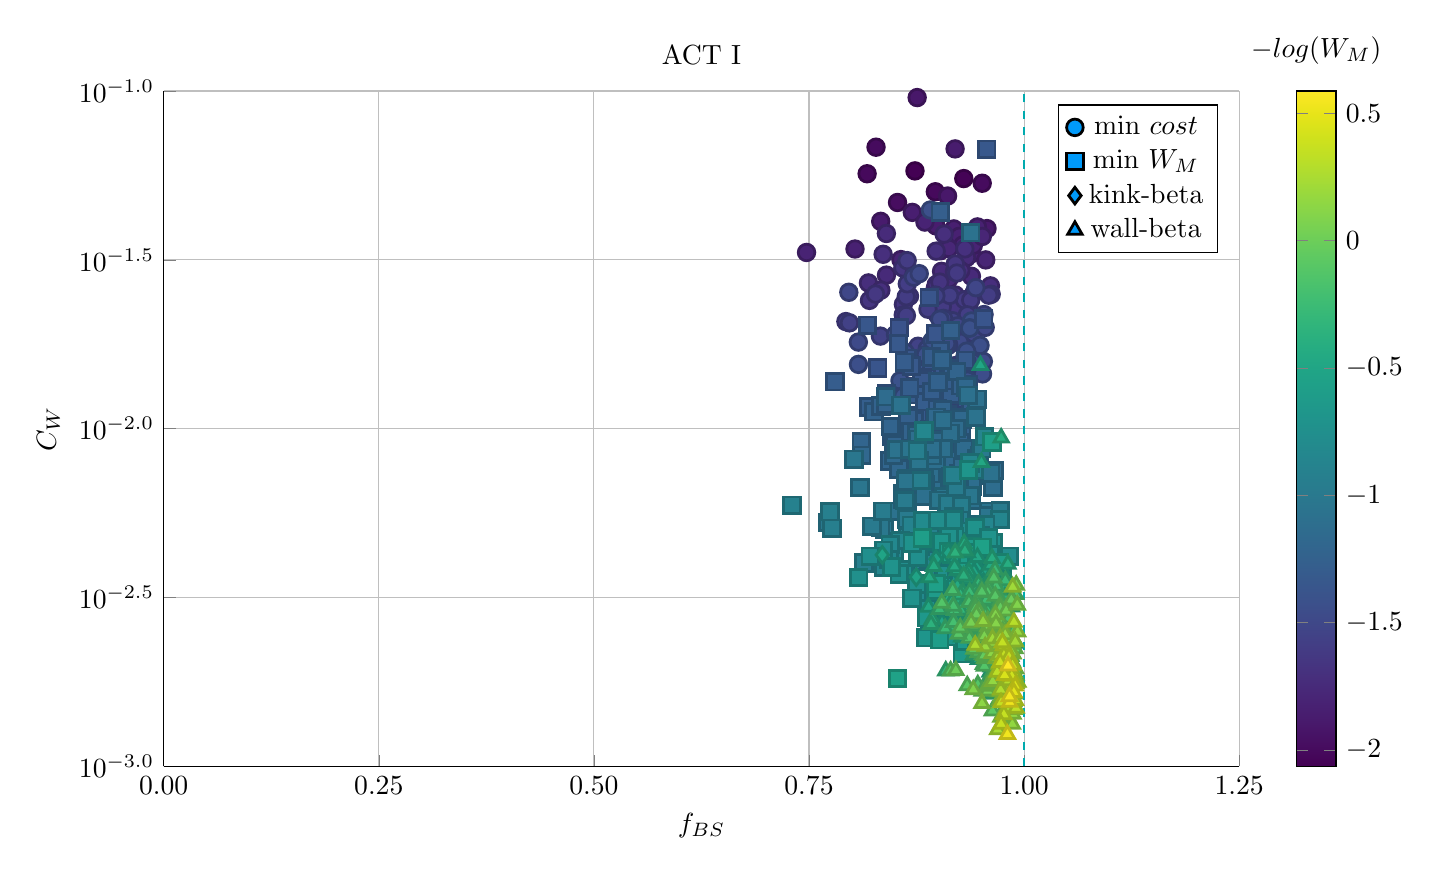
\begin{tikzpicture}[]
\begin{axis}[colorbar = {true}, height = {101.6mm}, ylabel = {${C}_{W}$}, title = {ACT I}, xmin = {0.0}, xmax = {1.25}, ymax = {0.1}, ymode = {log}, xlabel = {${f}_{BS}$}, {unbounded coords=jump, scaled x ticks = false, xticklabel style={rotate = 0}, xmajorgrids = true, xtick = {0.0,0.25,0.5,0.75,1.0,1.25}, xticklabels = {0.00,0.25,0.50,0.75,1.00,1.25}, xtick align = inside, axis lines* = left, scaled y ticks = false, yticklabel style={rotate = 0}, log basis y=10, ymajorgrids = true, ytick = {0.001,0.0031622776601683794,0.01,0.03162277660168379,0.1}, yticklabels = {$10^{-3.0}$,$10^{-2.5}$,$10^{-2.0}$,$10^{-1.5}$,$10^{-1.0}$}, ytick align = inside, axis lines* = left,     xshift = 0.0mm,
    yshift = 0.0mm,
    axis background/.style={fill={rgb,1:red,1.00000000;green,1.00000000;blue,1.00000000}}
, colormap={plots}{rgb=(0.26700400,0.00487400,0.32941500), rgb=(0.27794100,0.05632400,0.38119100), rgb=(0.28291000,0.10539300,0.42690200), rgb=(0.28229000,0.14591200,0.46151000), rgb=(0.27619400,0.19007400,0.49300100), rgb=(0.26514500,0.23295600,0.51659900), rgb=(0.25042500,0.27429000,0.53310300), rgb=(0.23360300,0.31382800,0.54391400), rgb=(0.21813000,0.34743200,0.55003800), rgb=(0.20123900,0.38367000,0.55429400), rgb=(0.18555600,0.41857000,0.55675300), rgb=(0.17117600,0.45253000,0.55796500), rgb=(0.15772900,0.48593200,0.55801300), rgb=(0.14618000,0.51541300,0.55682300), rgb=(0.13374300,0.54853500,0.55354100), rgb=(0.12346300,0.58168700,0.54744500), rgb=(0.11948300,0.61481700,0.53769200), rgb=(0.12632600,0.64410700,0.52531100), rgb=(0.15014800,0.67663100,0.50658900), rgb=(0.19109000,0.70836600,0.48228400), rgb=(0.24607000,0.73891000,0.45202400), rgb=(0.31192500,0.76782200,0.41558600), rgb=(0.37777900,0.79178100,0.37793900), rgb=(0.45867400,0.81636300,0.32972700), rgb=(0.54552400,0.83803900,0.27562600), rgb=(0.63690200,0.85654200,0.21662000), rgb=(0.73088900,0.87191600,0.15602900), rgb=(0.81457600,0.88339300,0.11034700), rgb=(0.90631100,0.89485500,0.09812500), rgb=(0.99324800,0.90615700,0.14393600)}, colorbar style={title=$-log( W_M )$}}, ymin = {0.001}, width = {152.4mm}]\addplot+[scatter, scatter src=explicit, only marks = {true}, color = {rgb,1:red,0.00000000;green,0.60560316;blue,0.97868012},
draw opacity=1,
line width=0,
solid,mark = *,
mark size = 3.0,
mark options = {
    color = {rgb,1:red,0.00000000;green,0.00000000;blue,0.00000000}, draw opacity = 1.0,
    fill = {rgb,1:red,0.00000000;green,0.60560316;blue,0.97868012}, fill opacity = 1,
    line width = 1,
    rotate = 0,
    solid
}] coordinates {
(0.8731583161087341, 0.057989258974827255) [-2.064962192389615]
(0.9298987639499251, 0.05502891594035146) [-2.050664082112704]
(0.8175467269590015, 0.05687405434298921) [-2.011767848487962]
(0.8968400727254129, 0.050297633592903325) [-2.009622310352661]
(0.8278998542362663, 0.06815552403146177) [-1.9979243426522733]
(0.9513172575512551, 0.0533071875450231) [-1.994929116630603]
(0.8528960525907812, 0.0467551640065516) [-1.9816591878685617]
(0.9110472238863242, 0.048856385398415615) [-1.9009357710890913]
(0.8756963278874996, 0.0955979106687745) [-1.9008410294477762]
(0.9568899267308207, 0.03913936102967274) [-1.8936707664226742]
(0.9038182735666613, 0.1016010514296217) [-1.88521103333311]
(0.8333207346473064, 0.04110929026091933) [-1.880964135698036]
(0.9197980139432043, 0.06737330593861776) [-1.8704830664747163]
(0.8974258881767438, 0.039880718652559814) [-1.8671602945516401]
(0.9272334069505606, 0.03552984785224197) [-1.8618595778785045]
(0.8700423982602555, 0.04370244723091091) [-1.8536550241998961]
(0.896264080513227, 0.04394725128364261) [-1.847107537048139]
(0.9182912055110312, 0.03904834505521419) [-1.845402906369208]
(0.9387755804676575, 0.03298266782702717) [-1.8299247064069584]
(0.9457850749264366, 0.03958498907028018) [-1.829338701662785]
(0.8034547513068042, 0.03404367677522339) [-1.8264739776199668]
(0.9246342918025143, 0.03712165869616768) [-1.8254736433338]
(0.9287361879267101, 0.03498163225660961) [-1.8213905780263324]
(0.8847474436704043, 0.04090408182009932) [-1.8110274827797526]
(0.856795859521427, 0.03167659938041034) [-1.8095831862560878]
(0.7471314354367964, 0.0332541407704371) [-1.8081577018045512]
(0.9410251229466832, 0.034919301353402016) [-1.8052282629113163]
(0.9553924992121228, 0.03160954199142242) [-1.794038121640695]
(0.9027109137951399, 0.03363661760525415) [-1.7922769049476923]
(0.9514525624218795, 0.03709266074378335) [-1.7862000983802733]
(0.9257525573046983, 0.03034628787303085) [-1.7852152332211932]
(0.9126142462724679, 0.03418438821960477) [-1.7772380652900426]
(0.9137711281814827, 0.028893150793615218) [-1.762233286346124]
(0.9229419485607372, 0.029679536940788936) [-1.757619916562725]
(0.9387544327064793, 0.028272317581563573) [-1.7541482977205345]
(0.8399908446535905, 0.028494444671935192) [-1.74919856251915]
(0.9330063198718748, 0.032094980075716116) [-1.747084370881807]
(0.9063829544808711, 0.027966816127232584) [-1.7470546081344984]
(0.8399078918577088, 0.03785249464890645) [-1.7442108348393488]
(0.9126714878088179, 0.027768727927201312) [-1.7420526933193456]
(0.9040493373469549, 0.029239023742660956) [-1.7395327755770893]
(0.9263873900569953, 0.02939344172802083) [-1.7194177486385185]
(0.8190620873895971, 0.027016419839008144) [-1.719386672725069]
(0.9608485147869371, 0.026478979134740822) [-1.7169068826642142]
(0.89672100112121, 0.02601353823911718) [-1.7158560236705473]
(0.8335103664153296, 0.025717415997762467) [-1.7110377836485957]
(0.8361586338341608, 0.032841764983913675) [-1.7108276685719623]
(0.9070013488697205, 0.03768314208183477) [-1.709665884336222]
(0.9311210648665087, 0.03408240796385454) [-1.6986723169730482]
(0.8977814047825817, 0.033552619629254835) [-1.6917720816198454]
(0.8979339043288382, 0.026734133388752808) [-1.6830702313615284]
(0.920096146584318, 0.024877717887061637) [-1.6818639287776478]
(0.9190311076672922, 0.02919080947335078) [-1.667258093217262]
(0.902083744032784, 0.027165378557205796) [-1.665200843447988]
(0.8202655212580311, 0.023985969206987357) [-1.66217138739501]
(0.9379149059771016, 0.024369099798012727) [-1.6616987570129709]
(0.8590574607971557, 0.029926873126084393) [-1.6608624949428865]
(0.8597162435331946, 0.023350604040071967) [-1.6542636311884442]
(0.9185584139892619, 0.022733615388835223) [-1.65363376409944]
(0.9200377378936719, 0.03074573955404929) [-1.6499261984079694]
(0.8989974045287558, 0.021769443299714454) [-1.6484233463349593]
(0.8718753959829374, 0.02860848134593445) [-1.6470118901263007]
(0.9418850072877972, 0.025250245321948275) [-1.6438624547347034]
(0.9366435359764497, 0.022365397187800617) [-1.6410421830745392]
(0.8272649318479791, 0.02504410573519034) [-1.6395041975177727]
(0.8668228410582832, 0.024666593634892982) [-1.6243573447802595]
(0.9217351814736208, 0.028901356853889247) [-1.6188313334564102]
(0.8968900959049646, 0.024870707244338257) [-1.6157329420330897]
(0.9049171939361385, 0.022969634317882806) [-1.6146571362099007]
(0.9307115846083037, 0.024077156878874784) [-1.614148731181496]
(0.9379312484272587, 0.02402881672676728) [-1.6095005691221438]
(0.9477409900819321, 0.0213102395674736) [-1.6092867324036153]
(0.9128640642999587, 0.020843342235322113) [-1.606635632554758]
(0.9617530768801122, 0.025003512509316483) [-1.606526739230697]
(0.8641075780272186, 0.03145376067268257) [-1.6054664027569479]
(0.7928641998948353, 0.020759493215449603) [-1.6036698390910544]
(0.8630240833375084, 0.024586269311698983) [-1.6025929165372244]
(0.8899699098575933, 0.02396900141580778) [-1.601873650665826]
(0.8595397653225256, 0.02173039511371947) [-1.6001281654735064]
(0.9588881971051215, 0.024851813061130205) [-1.5927988322260167]
(0.8642522328187694, 0.026860543755753686) [-1.5904529771214546]
(0.9134881848837252, 0.024815855265830314) [-1.58811206678891]
(0.8882619509730663, 0.022585530362625818) [-1.5852343487621334]
(0.8631856102877079, 0.02162169573243782) [-1.582687569840729]
(0.934056025980493, 0.02173125537760968) [-1.5805683995222133]
(0.7970138681074869, 0.020578686019115836) [-1.5616593837754646]
(0.8974438078752208, 0.0247399675666878) [-1.5545497681585543]
(0.9168089411359047, 0.02087834014908712) [-1.5504546678365727]
(0.8766721420501833, 0.01754547485137827) [-1.5489678431306624]
(0.8329698462406033, 0.01880088916330476) [-1.547222990629499]
(0.9313401534450555, 0.017954533760819902) [-1.5437410994768777]
(0.9063113702518492, 0.021211686613504643) [-1.5255698667472164]
(0.871445793631103, 0.028101067905464787) [-1.5206640942520917]
(0.9397631726706575, 0.018515106277898145) [-1.520578888956828]
(0.9077584139943392, 0.018879475562532277) [-1.5201607060653763]
(0.9227664842238432, 0.020162124791840028) [-1.517243514284296]
(0.9412253367039378, 0.01912604393689236) [-1.516001511335505]
(0.953452460582578, 0.02177699641289885) [-1.5127243295363797]
(0.9438615045031515, 0.02615640746740752) [-1.511222347964319]
(0.7962888966851867, 0.025345623651159097) [-1.502701591213217]
(0.9547380811291167, 0.019956615828691068) [-1.4983595788523634]
(0.8505719985854386, 0.01901365472017092) [-1.4975433274881913]
(0.899430644463361, 0.01625632266260828) [-1.4955435878672778]
(0.9201283417538595, 0.01537976653434252) [-1.4952511123493635]
(0.9309774985170253, 0.01624903115292776) [-1.4946977016701204]
(0.9376439198751291, 0.01616057272154418) [-1.491361147189787]
(0.9048534492341767, 0.016312938747661723) [-1.4862110854022101]
(0.925277958000399, 0.018052944734037228) [-1.481891473964466]
(0.9003094838292903, 0.017937749457507764) [-1.4799320170752728]
(0.8781116629474472, 0.028777552856445426) [-1.4795268228707887]
(0.9124042050421236, 0.017703624284785665) [-1.4795161068178337]
(0.8874100536029459, 0.017229927300776254) [-1.478794127235364]
(0.9299945195152068, 0.015225640153675678) [-1.4782749606324128]
(0.9161525972420332, 0.01946493284584485) [-1.4776976554667125]
(0.807334203101037, 0.018049212942760347) [-1.4759943912462838]
(0.9526456571529169, 0.015822574957211174) [-1.4744008984669785]
(0.9020920748075824, 0.021091946279007116) [-1.4733664186274853]
(0.921096776641852, 0.014982074855591734) [-1.470256415712286]
(0.9197524753995123, 0.014601174892861163) [-1.4657264924078404]
(0.9100402267973169, 0.017519770324100396) [-1.4622648103665985]
(0.9105130508409129, 0.01870406946961632) [-1.460868219021949]
(0.9204517436104007, 0.014392434992574372) [-1.4591279030736708]
(0.9032916286327085, 0.015543275856823037) [-1.4545703062138304]
(0.9098830294136144, 0.0178630357754997) [-1.4542955403831663]
(0.8618675014440598, 0.016835249428121063) [-1.4541997747641515]
(0.9516794080259597, 0.014530439682258098) [-1.4536072075076547]
(0.8074486816468343, 0.015504579589192491) [-1.4354993828498328]
(0.8773929747525714, 0.01586953423288717) [-1.4354866486000943]
(0.9487796918474358, 0.01764532719276209) [-1.4338583259741084]
(0.8951064297729344, 0.014716680911382386) [-1.4312674151204707]
(0.9387703969701673, 0.020843842366528337) [-1.4287189021457418]
(0.9331988731571469, 0.01696521637728643) [-1.4273925553382794]
(0.8670248952645595, 0.013340097264397483) [-1.4261610258499517]
(0.8911158581027104, 0.04442496675209589) [-1.4254440140277673]
(0.8854310169804341, 0.016560321493328565) [-1.42482226273413]
(0.9402601091187515, 0.015724531625960336) [-1.4225696979479532]
(0.9366331162927167, 0.019897722591771878) [-1.4120206972836251]
(0.9367488229696038, 0.01984475440507257) [-1.4098371032229988]
(0.8557087953810512, 0.013870037469952114) [-1.405975517390751]
(0.9336191151312027, 0.01581527557473546) [-1.4043018072199474]
(0.8931481570105053, 0.018214076204701567) [-1.4008019722945715]
(0.934367626111147, 0.013913111202702319) [-1.4005031963379073]
(0.9006796543319567, 0.015224038090080667) [-1.3999492210183218]
(0.8593933801817952, 0.012496931004535753) [-1.395557363349914]
};
\addlegendentry{min $cost$}
\addlegendentry{min $W_M$}
\addlegendentry{kink-beta}
\addlegendentry{wall-beta}
\addplot+[scatter, scatter src=explicit, only marks = {true}, color = {rgb,1:red,0.00000000;green,0.60560316;blue,0.97868012},
draw opacity=1,
line width=0,
solid,mark = square*,
mark size = 3.0,
mark options = {
    color = {rgb,1:red,0.00000000;green,0.00000000;blue,0.00000000}, draw opacity = 1.0,
    fill = {rgb,1:red,0.00000000;green,0.60560316;blue,0.97868012}, fill opacity = 1,
    line width = 1,
    rotate = 0,
    solid
}] coordinates {
(0.9271167760173109, 0.012445200437289321) [-1.3948646368052584]
(0.8549191496769539, 0.019927789901543477) [-1.3939537522252607]
(0.8799693920666783, 0.01314653896174034) [-1.392720101640072]
(0.8840883019018607, 0.014634720837625735) [-1.3866843034020317]
(0.9282463743720426, 0.013531122619790758) [-1.3787415633888773]
(0.8297318245194182, 0.015141818780145063) [-1.3757535398176242]
(0.8899071840495214, 0.024471157047317834) [-1.3752064107168462]
(0.9035475853680445, 0.014228443732750187) [-1.3749098088959892]
(0.9529741929254569, 0.02110676259399258) [-1.3739849131883028]
(0.93235118554593, 0.012256911562073732) [-1.3738531102934994]
(0.9014172243392794, 0.01330678684829131) [-1.3663541792461127]
(0.8778691210417414, 0.012962838848090586) [-1.3656599999201575]
(0.8969519049829034, 0.019050032640328597) [-1.3610117218468736]
(0.921562044788768, 0.01466611566297692) [-1.3573180864248318]
(0.864127365726556, 0.01616266376516514) [-1.3539978288520549]
(0.8180300548996796, 0.02022915729296448) [-1.3526036033103022]
(0.892574653228103, 0.014902347651238618) [-1.3518512539407643]
(0.8859492948655946, 0.01417644155990844) [-1.3492681452505735]
(0.8815164284149091, 0.013855965560709034) [-1.3352848695692758]
(0.956613991688453, 0.06723687686431194) [-1.33496858373192]
(0.8690737446612168, 0.015329274535082153) [-1.3328072948817369]
(0.8539133069876077, 0.01784511293289267) [-1.3313031998767464]
(0.8979877157834256, 0.011330055498166416) [-1.322748849742168]
(0.8397096010237105, 0.012679730072722432) [-1.3201016347693193]
(0.9215237604303135, 0.010156176015821517) [-1.315112649155682]
(0.9318984227066295, 0.01595337289689437) [-1.3137236413304165]
(0.8968767088385567, 0.012247545212491192) [-1.3091528292933776]
(0.876709873475441, 0.010892962462246563) [-1.3069473000965746]
(0.8735967833955901, 0.012601150633741464) [-1.3031541960229396]
(0.9025134685769323, 0.01697434802243184) [-1.2931806668520078]
(0.78038272871762, 0.013783864423757071) [-1.292511856848582]
(0.9350737398239659, 0.013475298350403871) [-1.291824809841371]
(0.8849689255593775, 0.012027127277753598) [-1.2898768957519178]
(0.860694823617397, 0.01571361767672998) [-1.2891587449819788]
(0.8926973187110631, 0.016322351172723598) [-1.285228192005334]
(0.8670116920112156, 0.013183257245795298) [-1.2828328944136962]
(0.9150950258835746, 0.012671641181110452) [-1.2825421072988568]
(0.9105634519289036, 0.010985300395990126) [-1.2800431569731807]
(0.9383400775725146, 0.011814811005805458) [-1.2782446441540516]
(0.913996516900395, 0.013863201694102639) [-1.2775473203773224]
(0.9121820439610082, 0.015027301664507256) [-1.2767406237155188]
(0.8723989867889326, 0.010547820414817374) [-1.2761629204758234]
(0.8902896550731525, 0.009931862296416103) [-1.2758557981370644]
(0.9158421037667931, 0.009498142916512152) [-1.2757288295353457]
(0.8925383407041332, 0.012893329705558294) [-1.2744847837776876]
(0.8192563180348535, 0.011606796760736388) [-1.2735549705057247]
(0.9161057579223539, 0.01475971281582095) [-1.2726652036752184]
(0.9025687723545689, 0.04385064317226166) [-1.2725563531490864]
(0.9176423466313344, 0.00956494266353577) [-1.2722662263080966]
(0.8991796141625694, 0.01145377372543799) [-1.2700642653169505]
(0.920538508471723, 0.010133330755881341) [-1.2679487567038392]
(0.9165797234269246, 0.009123134682627944) [-1.2616514169448798]
(0.8634478673767971, 0.009795622872305737) [-1.2594613969180772]
(0.8652451113775445, 0.01079410220229538) [-1.2586087657706206]
(0.8974734735996593, 0.0088934936775186) [-1.2559318752922384]
(0.8972097836781053, 0.00878637495619299) [-1.2524032337696909]
(0.9146956817162654, 0.01954536936309829) [-1.2500915845956104]
(0.9266577237247744, 0.013401347258256273) [-1.2491939573401372]
(0.9060566912781703, 0.009287974505863453) [-1.2465820537241712]
(0.8461463841435856, 0.009508338508488968) [-1.243935477994714]
(0.9180394857798562, 0.009032887794110376) [-1.240347841326793]
(0.8562897903410046, 0.008840699433936929) [-1.2384200469490936]
(0.9157222626166746, 0.008939458902182977) [-1.2370382372338191]
(0.8774564802835889, 0.009500681442262262) [-1.234594616796923]
(0.8997140678463201, 0.013750191876996646) [-1.2345143468522275]
(0.8255430755693288, 0.011226325606846698) [-1.2333943003160397]
(0.8338112522107382, 0.011680936250442807) [-1.2317476546541377]
(0.8685627242411781, 0.009765734724622308) [-1.2309520865359098]
(0.8971615157301666, 0.010568167602651573) [-1.230822839476929]
(0.838843805052853, 0.011811831633915183) [-1.2301871906487212]
(0.8789107801666443, 0.00916985873364138) [-1.2298215185804844]
(0.8919234914358547, 0.008206632432567867) [-1.2262871207474173]
(0.9214414379326734, 0.008184707349761693) [-1.2251252918595636]
(0.9275904428089702, 0.009543389942473697) [-1.2247092653793519]
(0.9143231802086956, 0.008412326051837992) [-1.2226672824447191]
(0.9216123853497962, 0.014763516356953353) [-1.2220223430792259]
(0.9044002301485325, 0.01597138256674089) [-1.219978616872189]
(0.9027130017667216, 0.00839744989573872) [-1.219457473300232]
(0.9211645176611111, 0.010746093594156849) [-1.2188777190787354]
(0.8786258539538101, 0.008033832445301942) [-1.2169302951859435]
(0.8494484079850726, 0.008975990584934701) [-1.21686127758645]
(0.9221310289995527, 0.009398677017548424) [-1.2167616565149533]
(0.84466182771518, 0.010149128207773273) [-1.2150613565699149]
(0.9208861119140008, 0.008396583729988576) [-1.2136335595316654]
(0.9053639683207135, 0.01140115444851449) [-1.213449396676557]
(0.9018392826470298, 0.00807858566271283) [-1.2090424219749658]
(0.8107793492157458, 0.009150247244763429) [-1.2068811791719494]
(0.9260034079845344, 0.00910352225246922) [-1.2043566377787012]
(0.8442941324782789, 0.008030436201599676) [-1.203115426690566]
(0.8621899253038897, 0.00829525893430832) [-1.2026712887263624]
(0.9475382029731105, 0.0076660148584983805) [-1.1966917975345508]
(0.9152752571057894, 0.010646380662135389) [-1.1947338618724224]
(0.8593153099539642, 0.008370016806452012) [-1.1927672386559536]
(0.8544491568392304, 0.007597051992083297) [-1.1848263349710841]
(0.8757227850487023, 0.009575551810758922) [-1.1808013668049147]
(0.9251889351463798, 0.007741558979980694) [-1.1794231767577772]
(0.811212783417515, 0.008342037909753687) [-1.178329489639351]
(0.9043967242186975, 0.01061614690368138) [-1.1776120518997013]
(0.9187473583725516, 0.008028594314197455) [-1.1770966259473905]
(0.9325685727720403, 0.013299033663900294) [-1.1736537021823468]
(0.8904003702289742, 0.008292790623650929) [-1.1709553925305785]
(0.8482856059746025, 0.008348409776511478) [-1.1702773251540795]
(0.9134364460032778, 0.008067808434749702) [-1.167112460757148]
(0.9244771021986321, 0.007367175811164478) [-1.1651375230967302]
(0.9279526851295172, 0.010664194028670942) [-1.164965492702215]
(0.8973994172179647, 0.010811857237065516) [-1.16397652023692]
(0.9394191821156371, 0.007049158619545943) [-1.160208221592745]
(0.9265691326442036, 0.007024176248113807) [-1.1587174467250145]
(0.9280658506320641, 0.007717544771526665) [-1.1570209420480233]
(0.9303231791026377, 0.008736514143459023) [-1.1478957642324041]
(0.9006608632246583, 0.009218200163918491) [-1.1469002727681683]
(0.9411405362226928, 0.007253865516894526) [-1.1400875045234886]
(0.9650109382613667, 0.007524944567097975) [-1.1391691710531666]
(0.8391428834450059, 0.012439153670574864) [-1.1379833555384578]
(0.9262309554101665, 0.0069967893818347416) [-1.1377170826120309]
(0.9208209619324543, 0.010002872629106504) [-1.1340145582937184]
(0.9637544328450613, 0.006715015712432569) [-1.121639283140209]
(0.9400709731105008, 0.006729229846129435) [-1.119539806519794]
(0.9014204193264993, 0.00641032554112888) [-1.1190022218812188]
(0.8923890653126869, 0.0073365166963547295) [-1.1185629451884402]
(0.882251161202865, 0.009102128960090845) [-1.1149656449984597]
(0.9018049683243878, 0.006567068570130298) [-1.112782188839356]
(0.8853454131125228, 0.006812914645648147) [-1.1117603631555923]
(0.9391048518724179, 0.006254604192766126) [-1.1083219728450635]
(0.87681385329431, 0.009301357270274212) [-1.1068629047281389]
(0.9244645109147069, 0.006851310091732623) [-1.1063474773659798]
(0.9141312650810365, 0.009696451234501371) [-1.1001422615629064]
(0.8978057921219315, 0.008046176359548657) [-1.0997982629203031]
(0.9209594912343368, 0.0061171437643153005) [-1.098670828295362]
(0.9054893907504951, 0.010596545096731845) [-1.0986241378865482]
(0.8877315508685263, 0.008577289597829926) [-1.0966387184251443]
(0.9452449245553554, 0.008169596287759642) [-1.0964883993749868]
(0.9132214581978662, 0.007121767916062895) [-1.0945790180182455]
(0.9150525541207138, 0.007187659319073351) [-1.0926081998530923]
(0.9058219953417993, 0.008724343791351657) [-1.0921043707901013]
(0.947802134523662, 0.008329953635747183) [-1.0913882990792323]
(0.8933038303627091, 0.008322658254688352) [-1.0910813694377977]
(0.8833011988886175, 0.006304319577189367) [-1.0901679951720686]
(0.8929811603643258, 0.008690684170777426) [-1.089367091074117]
(0.9145080171681728, 0.006583412820443741) [-1.0891727565542524]
(0.9453955802025471, 0.012211134116054666) [-1.0880555961261078]
(0.9350836555291349, 0.012548811552576346) [-1.086936622940194]
(0.8589137292175502, 0.0064141553047330985) [-1.0863825614156546]
(0.8836849391290048, 0.0071097507635516565) [-1.0751044594117714]
(0.9610484127018367, 0.007374731494224653) [-1.0737380492352289]
(0.9389985571359603, 0.006145695209859947) [-1.070616517292677]
(0.9379977248665374, 0.03802674603286673) [-1.069913767001807]
(0.9213417260466619, 0.005970957417198659) [-1.0690750828665614]
(0.8548598275117848, 0.005698307632946107) [-1.0678680329287458]
(0.8522098522639113, 0.008661247168726348) [-1.0674080884082333]
(0.9439305152507809, 0.010817648781713476) [-1.0654260064541108]
(0.8567559640448742, 0.011722467292523471) [-1.065193792118979]
(0.920196530172107, 0.005714167148636787) [-1.0629774807936423]
(0.8640983076229167, 0.00711622998416048) [-1.0618319340909603]
(0.8592709820297094, 0.006173537615536586) [-1.0600703364411528]
(0.8583017671103392, 0.006233626320552047) [-1.0598646582955382]
(0.8841777194347801, 0.009626390481863662) [-1.0577742882294356]
(0.9122660365302591, 0.005936752040130104) [-1.0548470198030315]
(0.9587389518915752, 0.0056904737038728165) [-1.0541768592648042]
(0.9108628990594947, 0.006032343424076769) [-1.0487285499150356]
(0.9584682101650461, 0.005521470027251347) [-1.0462570464475487]
(0.9173449278328639, 0.0070995694405497235) [-1.0460234006078977]
(0.8628552558040238, 0.007007981654725635) [-1.0452759731087355]
(0.8668509459578728, 0.008683290730999459) [-1.0445119467109005]
(0.9105499342272777, 0.0055299967565469975) [-1.0384000215358105]
(0.8638198429570266, 0.005998532550171044) [-1.038305441802928]
(0.9208568729989152, 0.00528018761380554) [-1.0347714947666997]
(0.8093436631281515, 0.0066967057377454575) [-1.0308440378796533]
(0.8779579874197121, 0.008036724741540775) [-1.0305940259463149]
(0.906869624199176, 0.0062926123227946265) [-1.025221203256898]
(0.900789950373511, 0.0061379044438670954) [-1.0179285117664867]
(0.9375398126250842, 0.006334972879805434) [-1.0176162076457083]
(0.8024708047377667, 0.008112959181062486) [-1.0169975029536151]
(0.8375801334207545, 0.005049047597761542) [-1.0141985821053012]
(0.9324121317714827, 0.005064450169828918) [-1.0124724404696706]
(0.833350555301248, 0.005088814715939496) [-1.0103391716309778]
(0.9513980291319009, 0.004962576605235948) [-1.001427881081934]
(0.9271181895900452, 0.005884671104664021) [-0.9993824808081277]
(0.9099503941424658, 0.005418776785282774) [-0.9941634259261274]
(0.7720181731709707, 0.005280889139989257) [-0.9936318009336389]
(0.9505960598919263, 0.008723874856120134) [-0.9908776434018548]
(0.8943895369875628, 0.00491490634866398) [-0.9892483689799706]
(0.9417125317554466, 0.004961736780563244) [-0.9883704068819422]
(0.8233418299878267, 0.005137841489967903) [-0.9826953741849849]
(0.8934787894059866, 0.004754734001145322) [-0.9811279654336956]
(0.9403526918266536, 0.004647560340984803) [-0.9793471772630553]
(0.9723583859212274, 0.005703060525950649) [-0.9776886993834442]
(0.8611589318505539, 0.006131488667777248) [-0.9769724317666026]
(0.9410654966962836, 0.004745131633522655) [-0.9769267723302241]
(0.9399901789088603, 0.005212687153670182) [-0.976835072767447]
(0.9567462107415136, 0.0046034051010616075) [-0.9752013352458598]
(0.8636848687114632, 0.005388412680270176) [-0.9746899157531883]
(0.9075358432123548, 0.0045774223618013105) [-0.9727431242330735]
(0.9447314559272533, 0.004552413603526284) [-0.9703638528440552]
(0.9414650087723526, 0.004525683131963228) [-0.9678062840180223]
(0.8357492652861911, 0.005692276004720247) [-0.9676725483675591]
(0.9005181216481226, 0.004498229501695765) [-0.9651637505902915]
(0.9206601577164616, 0.0067323238980037245) [-0.961259110326393]
(0.9083905113541957, 0.004736392493078221) [-0.9563360314157324]
(0.9301172641173069, 0.004854184151533866) [-0.9558845590306136]
(0.9194947604180831, 0.004573806166601441) [-0.9532763546481751]
(0.941953192362469, 0.004793440229443098) [-0.9511957035164516]
(0.8806212569679992, 0.004877743614014347) [-0.9508596108314747]
(0.9329503575731299, 0.004350998493140003) [-0.9507110729257874]
(0.911454495262883, 0.006001608290604688) [-0.949683613164744]
(0.8879558751803653, 0.004290521076860756) [-0.944632180714094]
(0.9184319984465406, 0.0043767749507575135) [-0.9438112967734156]
(0.9271750473353343, 0.005920276984804288) [-0.943373672256531]
(0.9105611701686498, 0.005363684807666859) [-0.940593168106771]
(0.7767420971999245, 0.005068452256325543) [-0.9348384496596517]
(0.9038987139905713, 0.0049263739241811695) [-0.9347532688355591]
(0.8759023691861031, 0.008601524715605227) [-0.9342019527454238]
(0.8549702147859954, 0.004640144515353838) [-0.9329513708540818]
(0.8803983184588043, 0.0070257271621669455) [-0.9316183752161744]
(0.9259016565967537, 0.005358998371858679) [-0.9286370269103483]
(0.9616193719002063, 0.00413086470485901) [-0.9281631121842467]
(0.8741693390281038, 0.004765635288464319) [-0.9277381641373396]
(0.8490865721871718, 0.0040620137628436526) [-0.9208635313499342]
(0.8814246252669371, 0.0040488305993979234) [-0.9194517468501666]
(0.7743381134865549, 0.005678582545669974) [-0.919260894818004]
(0.8140652070684143, 0.0040019705744028635) [-0.9143960307834678]
(0.8956167430991006, 0.005105193674380799) [-0.9143339304202898]
(0.923307386920103, 0.004202079139621733) [-0.9117699942132877]
(0.9090872570665293, 0.004239308070694324) [-0.9111513250328139]
(0.9186515311897197, 0.005481038677141083) [-0.9106272870974846]
(0.8651143294304927, 0.004774812507931078) [-0.9099002226686804]
(0.9212576993079015, 0.003944067969601837) [-0.9080665243282653]
(0.9288275574225838, 0.004788438955058866) [-0.9070188756981697]
(0.9170518000340987, 0.007279773971914604) [-0.9043577198452432]
(0.9063089707483508, 0.004734796732954004) [-0.9038476343568516]
(0.9417824172363041, 0.007562673512498189) [-0.8994655785667166]
(0.7301551050698963, 0.005931441653675227) [-0.8989662338456113]
(0.9221426597591885, 0.003977844960348454) [-0.8984429206195617]
(0.924185246169707, 0.003852765847835788) [-0.8978947560680902]
(0.9113180230450746, 0.003844792233549059) [-0.8969950165065196]
(0.915991064143121, 0.0038178462182025725) [-0.8939405705697983]
(0.9184306750512461, 0.004330108994839308) [-0.8939109716982566]
(0.8906172680403811, 0.004992871742589902) [-0.8925148817167516]
(0.8413904437613173, 0.003881299542388103) [-0.8913217265447397]
(0.9127227138669043, 0.003772719391214399) [-0.8887766390600081]
(0.908016086635955, 0.003988034719656209) [-0.8874455768491046]
(0.9229973452568307, 0.003741945120882656) [-0.8852195535706585]
(0.9042193119427263, 0.0039058028277476073) [-0.8842325860222515]
(0.9626746195716175, 0.0037216011971632503) [-0.882851972521222]
(0.9136705428571793, 0.005315372520692716) [-0.8819881369375219]
(0.9255182413778642, 0.004466619068705632) [-0.8808109550697729]
(0.9332929151781738, 0.004730802817477606) [-0.8806633070174894]
(0.9455320084521668, 0.005113228457075696) [-0.8805814649771261]
(0.9059749221374921, 0.004582507032171267) [-0.8799678258438864]
(0.8687604466888538, 0.005177586923248842) [-0.8768550082578233]
(0.906638161832524, 0.0037611740992579295) [-0.8726983150888058]
(0.9142503324644239, 0.003993806119831429) [-0.8703497234695906]
(0.9005945327194729, 0.0045270286179628335) [-0.8696853700725911]
(0.9125504162559055, 0.004726535412937384) [-0.8641851323647479]
(0.8894648886019335, 0.004089711851258383) [-0.8640642580417203]
(0.84906414633368, 0.004221088787393515) [-0.8560530688301973]
(0.9539183047560731, 0.009465725470453552) [-0.8558368077947285]
(0.8365167684350138, 0.003886605388747585) [-0.8512125553695333]
(0.9717681447799739, 0.005381883944145375) [-0.8506650866802525]
(0.9413045252603143, 0.0034368070052375275) [-0.8482772851581519]
(0.9371247405745184, 0.007913375166879979) [-0.8464932034376795]
(0.9553776236479619, 0.005205559212542438) [-0.8445031740165281]
(0.9335984452174588, 0.003401911815632122) [-0.8438451898892435]
(0.899362439922284, 0.0036969679593135867) [-0.8422027975238203]
(0.9073351601479548, 0.003987547217632283) [-0.8387200271046066]
(0.8562092207533517, 0.004668264864015146) [-0.8364691763469672]
(0.8837759321999247, 0.009844996004785781) [-0.8348845112947673]
(0.9527366094531792, 0.0042937690240102055) [-0.8334732362359846]
(0.9489776318197072, 0.004829578534215681) [-0.8314604487141729]
(0.9406793011442216, 0.0033045292752156012) [-0.8312317421172319]
(0.9066275099303774, 0.003944865613295989) [-0.8300993342247266]
(0.9525847470320502, 0.0036964164829665054) [-0.8257124339268005]
(0.8444119719816215, 0.004543282198622211) [-0.8240402889058517]
(0.8428732433620125, 0.004091458079546767) [-0.8237101255156289]
(0.8792038820199741, 0.0044798519520400275) [-0.8212814607963961]
(0.9128010485164441, 0.003865354216978021) [-0.8184309573457651]
(0.9408107529966464, 0.003517618433797349) [-0.8179460037153172]
(0.907201661370005, 0.004172133397045878) [-0.8177471845862596]
(0.9147419729006552, 0.0032035011715418273) [-0.8177470190925474]
(0.9341737972997356, 0.00486116253252262) [-0.8115196740923352]
(0.880427881452171, 0.003291086034139362) [-0.8109601097483452]
(0.9369616057293777, 0.003137434005415254) [-0.8086967395269018]
(0.9368507058055328, 0.004970208362256673) [-0.7960351903235757]
(0.8759951589174462, 0.004399209393210064) [-0.7927306784842179]
(0.8824674295611945, 0.0053371866278534704) [-0.7914765499147394]
(0.9379258499987612, 0.003498945953927069) [-0.789558366829936]
(0.9198630378378857, 0.0036511274139089086) [-0.7884146729758114]
(0.8944594126549716, 0.003059756391991388) [-0.780563955995713]
(0.8365394691215563, 0.004362695965775012) [-0.7773019949176746]
(0.9490480155902238, 0.0033800793800363477) [-0.7771403289080958]
(0.9131766240023282, 0.0038433908405004595) [-0.7759893078752428]
(0.9174522110836529, 0.005361590568500423) [-0.7757750986160458]
(0.9828063504707286, 0.004188332285621625) [-0.773903866721892]
(0.860373325745603, 0.003814507127921371) [-0.7720119659547495]
(0.916412698271093, 0.004563472793394545) [-0.7712260807781841]
(0.8993603428221363, 0.005353933823001906) [-0.763713355476829]
(0.9229671461890366, 0.00443577956251074) [-0.7611487713118793]
(0.9135746793667092, 0.0035425697821227136) [-0.7583244805207935]
(0.910163554471783, 0.004316533455984555) [-0.75431667125663]
(0.9530775482444933, 0.004013911959896482) [-0.7523987856492388]
(0.8765992248443446, 0.004167145198855743) [-0.7521837169110341]
(0.8211767177946366, 0.00419041579250737) [-0.7520281092582939]
(0.899188988809008, 0.004640432958808489) [-0.7480037221630257]
(0.9196475384979264, 0.004637571540936418) [-0.7479709949279421]
(0.941544518760215, 0.0029690205808463126) [-0.7433492218430673]
(0.8548068550317491, 0.00371133233538681) [-0.7429682997042104]
(0.9076295967230273, 0.0037176890833071395) [-0.742916937139166]
(0.9629606418977977, 0.003573548669295098) [-0.742391688221943]
(0.9132986441445263, 0.004342699202151464) [-0.7387214685527604]
(0.9425549117040624, 0.004120352722007335) [-0.7376833551276831]
(0.8876167102132334, 0.0029344519800280494) [-0.7361332571045444]
(0.9192007895561155, 0.0026407580062505036) [-0.7338507300143334]
(0.9190838352844859, 0.004642553663675521) [-0.7338020684083535]
(0.8076734375543824, 0.003625959959243182) [-0.7337899099402782]
(0.8755348906962087, 0.003471864499773886) [-0.7327475728465653]
(0.9192982155145527, 0.004787324827841368) [-0.7317731615704781]
(0.9128657943764739, 0.0032492446650530782) [-0.7295946657832332]
(0.9643502521670281, 0.004590135412859294) [-0.7278656799085517]
(0.9436063499469458, 0.002781573765952152) [-0.7275349704092896]
(0.9124911104830998, 0.004786847520366514) [-0.7260638209608133]
(0.8701208160624356, 0.0045831738993045434) [-0.7223530950014921]
(0.8903186381182336, 0.002706327638391427) [-0.7222465976506431]
(0.9221605488926754, 0.0038384358624846005) [-0.7206838995228373]
(0.8697565045491886, 0.0031485580487720824) [-0.7200286244342213]
(0.9304077214790845, 0.0025439466913436885) [-0.7176301464195668]
(0.9277282929298999, 0.0032994837811560433) [-0.7172574131133485]
(0.9083357619132455, 0.0029608346461731517) [-0.7146734939586027]
(0.9386095594667047, 0.0038416894509805963) [-0.7135338154993714]
(0.9622893760246558, 0.003978944435631734) [-0.7134219342397831]
(0.9244732248388806, 0.00294062590420396) [-0.7111824287105687]
(0.9074754137233341, 0.002616774757125684) [-0.7110478679106434]
(0.9283660526071763, 0.002703036682855945) [-0.7101349740556314]
(0.9333747341388989, 0.0038042134944218514) [-0.708793386355897]
(0.9430505809327492, 0.005100030907026268) [-0.7086868054853989]
(0.9427900983410764, 0.0029638877995658438) [-0.7060021380009439]
(0.9398200782334812, 0.00420966050281472) [-0.7051679285913526]
(0.9604861518997936, 0.004243872080162761) [-0.7047135863350958]
(0.9589708628544776, 0.004746158897630676) [-0.7042552774527877]
(0.8457887824363216, 0.0038984799726810644) [-0.7040543449813873]
(0.9446655949709295, 0.003681874907434521) [-0.7029065147187739]
(0.9255802437476592, 0.003518446922920876) [-0.7024908064183792]
(0.9430578726532933, 0.0031358132900712187) [-0.7020173640529951]
(0.9358114830098702, 0.0034846556769238916) [-0.7002858883929466]
(0.9154923073284251, 0.002420499336307095) [-0.6886136022852183]
(0.9487125552664237, 0.0030008632151973602) [-0.6883840449068117]
(0.9749351638619993, 0.0036390786158231932) [-0.6856303672495035]
(0.9354490208131545, 0.0075440190367227515) [-0.683929391159688]
(0.8861740952059259, 0.0024047709432785456) [-0.6820666452179769]
(0.9399550230633152, 0.003179486303873929) [-0.677506260008208]
(0.9172222823672502, 0.002743556277657468) [-0.6766480250628556]
(0.8971448208467913, 0.0033449553430014638) [-0.6742373084561588]
(0.9498796899572547, 0.003589950489194691) [-0.6693580918378859]
(0.9614003416076418, 0.0027885517140979043) [-0.6663261681981373]
(0.904051942834427, 0.004612234783079175) [-0.6640820182002938]
(0.8870769402218344, 0.002756794030954554) [-0.654540142215377]
(0.9145144637231343, 0.003011986481013787) [-0.6541170476368723]
(0.9386740677642995, 0.0023920692653461198) [-0.6479269306921259]
(0.9272166472611978, 0.002907917303840169) [-0.6474513086378696]
(0.9652245577162768, 0.003970372686667843) [-0.6471618340133566]
(0.9361938078592776, 0.004183393535167865) [-0.6464557691155365]
(0.9282205063877679, 0.0021562827004047414) [-0.645827839166682]
(0.9428246002353234, 0.003935863383612764) [-0.6392562670118296]
(0.9332729807874064, 0.0033071434441903505) [-0.6390324015661447]
(0.965299692734038, 0.0029382720604000773) [-0.6356690770784437]
(0.9307544297265398, 0.003213331172803855) [-0.6356557512792106]
(0.9020078833291566, 0.0034338634182182544) [-0.6319127156425483]
(0.9637226872809501, 0.0026258384701233024) [-0.6311782107023105]
(0.9311304196250344, 0.002344563264707828) [-0.6306618545653738]
(0.9362327301699095, 0.0043309424812136305) [-0.6294646208449958]
(0.9571595789927293, 0.0035648943963739244) [-0.6281694872206178]
(0.9373951586764807, 0.004473909353971782) [-0.623997332545462]
(0.9246735358540317, 0.003055298672515709) [-0.6239428210926011]
(0.9604091908555257, 0.0033667157021052925) [-0.6220841804266346]
(0.8970165492513017, 0.003322033041865016) [-0.6194634144361497]
(0.9463845319434011, 0.0026017333836386653) [-0.6157020019788386]
(0.963381254766795, 0.002981595770740583) [-0.6128668873662166]
(0.9386459319770583, 0.0029654442870923124) [-0.6087223349615605]
(0.9378475201084454, 0.0027835646988952733) [-0.6079986647506345]
(0.9662961539484464, 0.0035338295468618167) [-0.607409669430742]
(0.9676799600416237, 0.003208776600520151) [-0.6057755138787592]
(0.9548162111293393, 0.0024649747969395317) [-0.6023349029229402]
(0.9437686876752717, 0.00428654565390444) [-0.6021966320137805]
(0.9313542688063162, 0.0036421375219878684) [-0.601256050165278]
(0.9810116318859735, 0.0032082112461564497) [-0.6004710736804056]
(0.9210211525451228, 0.0033480033632593445) [-0.5989376185886022]
(0.9261414327388798, 0.004184088897695592) [-0.5988379503314065]
(0.9451747550689351, 0.0021588377429705994) [-0.5983904370889932]
(0.9603531355012247, 0.002371262429759035) [-0.5972702626291994]
(0.9145691707746888, 0.003153537233065522) [-0.5971677630195633]
(0.9332687303609898, 0.002738950954618617) [-0.5943817111698461]
(0.9017811764393036, 0.002374076549827175) [-0.5925805266117682]
(0.9529087666605505, 0.0035156750139523495) [-0.5892976849983818]
(0.8818050628541011, 0.004748358787901646) [-0.5871411238278668]
(0.9410709712036359, 0.0028576481981739026) [-0.5871026900807895]
(0.9118739529147474, 0.004310975115774645) [-0.5855555754858193]
(0.9270393774931934, 0.002622282088332502) [-0.582078933118425]
(0.9471345660347393, 0.0027290583320010026) [-0.5810302095860215]
(0.9709522317939191, 0.004011340237339877) [-0.5752080843644548]
(0.9373730580166739, 0.003188972111543657) [-0.5747894604151379]
(0.9625216290079742, 0.009121559432388153) [-0.5726182655122839]
(0.9328769641864062, 0.003781132407311784) [-0.5681761634850476]
(0.9477741047064356, 0.0035193905138756446) [-0.5675125713590323]
(0.897813303968198, 0.003476123369301586) [-0.563542896843953]
(0.9444020460316636, 0.003526213328274809) [-0.5617459654165032]
(0.9367882704708124, 0.0030283854486626957) [-0.5606455598520448]
(0.9591748673290499, 0.003698026746714474) [-0.5561768160153511]
(0.9161540099636023, 0.003037543717331452) [-0.5554794435604244]
(0.9544577117139241, 0.003123058961705477) [-0.5527929477248187]
(0.949948991371526, 0.003063222342257361) [-0.5501170234905265]
(0.9512932862322991, 0.004453634731593786) [-0.549388250021666]
(0.9704366682428202, 0.002634748468893335) [-0.5492540867532439]
(0.9706397193138688, 0.0029729026877479644) [-0.5480705365568839]
(0.9209369867443455, 0.002890688526532444) [-0.545336361217705]
(0.9727226532153145, 0.0029512333115660695) [-0.5441402349163921]
(0.9654875864077215, 0.0033237315785907802) [-0.5415522046162035]
(0.9153924411701821, 0.004254172680928966) [-0.5404988012673853]
(0.9438711844295444, 0.0028783860919469858) [-0.5391201246551751]
(0.8528119086554116, 0.0018217622549288588) [-0.5378589410507132]
(0.9399210599276655, 0.0029280615221428286) [-0.5375464729950068]
(0.9656845492175761, 0.003605866681887626) [-0.5363826507452838]
};
\addlegendentry{min $cost$}
\addlegendentry{min $W_M$}
\addlegendentry{kink-beta}
\addlegendentry{wall-beta}
\addplot+[scatter, scatter src=explicit, only marks = {true}, color = {rgb,1:red,0.00000000;green,0.60560316;blue,0.97868012},
draw opacity=1,
line width=0,
solid,mark = diamond*,
mark size = 3.0,
mark options = {
    color = {rgb,1:red,0.00000000;green,0.00000000;blue,0.00000000}, draw opacity = 1.0,
    fill = {rgb,1:red,0.00000000;green,0.60560316;blue,0.97868012}, fill opacity = 1,
    line width = 1,
    rotate = 0,
    solid
}] coordinates {
(0.9387315044574429, 0.0026801888273270944) [-0.5362477970958698]
(0.9188676920673408, 0.003015899524278956) [-0.5319316345767685]
(0.9402750910418581, 0.003937320309019732) [-0.5311726618261826]
(0.9497566997238739, 0.002676245927362068) [-0.5263288636267944]
(0.9578205337936164, 0.002870837451508785) [-0.5247247581053419]
(0.9377452621123799, 0.0036932959279301603) [-0.5234426911679817]
(0.9236521135109587, 0.0037417097390243918) [-0.5218292719861799]
(0.8746520089629003, 0.0036365094358458082) [-0.521460274671524]
(0.9465267456827315, 0.003836260132829497) [-0.5210413145984053]
(0.9414429637766969, 0.0035893000080833405) [-0.5203271708770874]
(0.8975678911738616, 0.004109858290155805) [-0.5199020238276453]
(0.95491686971008, 0.0037200592776891026) [-0.5183158834743817]
(0.9759243558794375, 0.0028015521912634306) [-0.5173345034609598]
(0.8351619950547207, 0.004230376861424109) [-0.515292403587272]
(0.911974433569001, 0.004287050052594506) [-0.512831160599956]
(0.9451890358998748, 0.00385875121306247) [-0.5125342981633305]
(0.9573604100369881, 0.0024821104525564698) [-0.5110529951676259]
(0.9255709718590797, 0.002644344245828979) [-0.5107257930504342]
(0.9014823759874409, 0.002951817009326848) [-0.5100450482708185]
(0.9342743233933991, 0.0036294488088753976) [-0.50815885357027]
(0.9386447741605193, 0.00293906318241377) [-0.5068673822722911]
(0.9434533574756855, 0.0033114367041341864) [-0.5065015706006631]
(0.9645103989085381, 0.00315022051140993) [-0.5028304672765428]
(0.965810101196494, 0.003265777243065683) [-0.5020774334996001]
(0.940852716473451, 0.002195233443131404) [-0.5006102606405294]
(0.9269508172989578, 0.0029561853413927267) [-0.4999881748262777]
};
\addlegendentry{min $cost$}
\addlegendentry{min $W_M$}
\addlegendentry{kink-beta}
\addlegendentry{wall-beta}
\addplot+[scatter, scatter src=explicit, only marks = {true}, color = {rgb,1:red,0.00000000;green,0.60560316;blue,0.97868012},
draw opacity=1,
line width=0,
solid,mark = triangle*,
mark size = 3.0,
mark options = {
    color = {rgb,1:red,0.00000000;green,0.00000000;blue,0.00000000}, draw opacity = 1.0,
    fill = {rgb,1:red,0.00000000;green,0.60560316;blue,0.97868012}, fill opacity = 1,
    line width = 1,
    rotate = 0,
    solid
}] coordinates {
(0.9637825785469384, 0.002418031031362927) [-0.498048892810302]
(0.9828868114547558, 0.0034404977503060406) [-0.4963542958643768]
(0.9417630512196451, 0.003776085604922812) [-0.49628974660312986]
(0.9492250000053065, 0.01540146473031375) [-0.4934359099515097]
(0.9528731459467576, 0.0035153091327000956) [-0.49249004910762223]
(0.9423833026459857, 0.002494247580013818) [-0.49140410679398333]
(0.9457792108846419, 0.00416125103061467) [-0.4852361666757575]
(0.9881577775397556, 0.0023204725608605052) [-0.4804115307603524]
(0.9684130895026871, 0.002093548495356325) [-0.4801206531671318]
(0.9317207652243386, 0.00284573975236386) [-0.47768993884134897]
(0.9045268350433837, 0.002672085055478309) [-0.47763997399503283]
(0.934107896081881, 0.0042968350893615405) [-0.47748483227356914]
(0.956153940041833, 0.0027283486462771588) [-0.47710934625073764]
(0.9504424943308272, 0.007954298543771714) [-0.47443162890256063]
(0.9653194212047426, 0.0034997930230070513) [-0.4730103351970393]
(0.9485975480554657, 0.003084116536456388) [-0.46957975685881903]
(0.8888799663257206, 0.002965009685568973) [-0.46566614748110147]
(0.9486063771337456, 0.0033818570105314436) [-0.4649012306603411]
(0.9370503936999514, 0.0027326785960835984) [-0.46367023078588027]
(0.9751148974972959, 0.0021589205831240984) [-0.4608405143654578]
(0.9674139205875375, 0.002909388047886919) [-0.4559980166467371]
(0.922320661557035, 0.003804219838416559) [-0.4557530150298407]
(0.9617531036033169, 0.0019740686546661367) [-0.4531031573331743]
(0.9720919152815786, 0.002865519155805154) [-0.45102557337314547]
(0.980962555274262, 0.0035904404442790834) [-0.4498801205421611]
(0.946983470396084, 0.0020770215253626836) [-0.44934749702523663]
(0.9611200201095378, 0.003946973381825038) [-0.44691387139898353]
(0.9423559591891613, 0.0021324454337363157) [-0.4467784211878218]
(0.9722802466644753, 0.0034454822663482288) [-0.44543367276420787]
(0.9783180452946528, 0.002782106060611568) [-0.4452644336485217]
(0.9196744854606606, 0.002683981555832874) [-0.4442292803657962]
(0.919083328393837, 0.003903022328021505) [-0.443911172249478]
(0.8898006726939861, 0.003625566982744672) [-0.4436886749023339]
(0.92242541783831, 0.0034353021273270624) [-0.4428673152256711]
(0.9431609264388685, 0.0029639232525875054) [-0.442238228799892]
(0.9358243168882298, 0.0037655549686147634) [-0.43652345648336177]
(0.9503286495330018, 0.00316522398873329) [-0.43264010832961963]
(0.9207873219189756, 0.0030700324868674126) [-0.4320972745079676]
(0.9377557419395087, 0.003176641543542351) [-0.42987155892029094]
(0.8949789010922767, 0.003915956445463101) [-0.4296439742036936]
(0.9759525328731052, 0.002390393629432453) [-0.4247534556148279]
(0.9356006610018043, 0.0036007806434798697) [-0.424149565057673]
(0.9574249801685056, 0.003539095491390182) [-0.4205236931986052]
(0.9275740991213478, 0.0024211809823555977) [-0.42019149809413414]
(0.9302760961483995, 0.004563891593018241) [-0.4197034422744706]
(0.9425672326920357, 0.0032856394117234847) [-0.41794543148337715]
(0.9760510560418263, 0.0027967003623514523) [-0.41678804196626223]
(0.9733626734052071, 0.00939464568044268) [-0.4165344070166825]
(0.9667677622156696, 0.0023850426517976657) [-0.41610390181296675]
(0.9811161937084777, 0.003976369722968889) [-0.41504401225288956]
(0.9627875479660791, 0.004131558509006773) [-0.4123238967763576]
(0.9682163110315346, 0.002480526294810785) [-0.41152198567356807]
(0.9213450026541719, 0.0027953596024665873) [-0.4112038942283755]
(0.948003368809075, 0.002908194002865418) [-0.40443861763435524]
(0.970824830278417, 0.0031509219796267978) [-0.40439477308945854]
(0.978413175175616, 0.00339721031225261) [-0.40338973957807817]
(0.9311897624930034, 0.004349911096016139) [-0.4030415600388741]
(0.9496201135347039, 0.003290400715978174) [-0.40289755527840704]
(0.9683050960972667, 0.0028030854340314122) [-0.4014505433547788]
(0.9584415756432187, 0.0034529644355774437) [-0.4001808646663969]
(0.9467228957774027, 0.003146073711407124) [-0.39739544195307136]
(0.966212109881682, 0.0022106236218850106) [-0.39694963709739944]
(0.9604928388260168, 0.0019035407229546452) [-0.3963062967743845]
(0.8932484709144216, 0.0027278955338643357) [-0.39516887549856156]
(0.9774347337184184, 0.0029116530286545247) [-0.3951332072545033]
(0.9619965305624404, 0.0021685930793473884) [-0.3941022330693172]
(0.9300294057368946, 0.0024151906231217376) [-0.3907955867090377]
(0.9672161397751312, 0.002518216932252145) [-0.38953420209200085]
(0.9199593546698408, 0.0027251737271486174) [-0.38868299787281246]
(0.9642814816569392, 0.002183317183672608) [-0.3871061422148591]
(0.9754991993658442, 0.0029833969525940494) [-0.38501115835920763]
(0.9530920288221355, 0.0026684516909069264) [-0.3845328258663582]
(0.9443562367823123, 0.0024879890917625298) [-0.3834242121013558]
(0.9623765466518088, 0.003655954697826326) [-0.3819367797682986]
(0.9326447166989683, 0.002488879500771219) [-0.37899373798674496]
(0.9720816671195145, 0.0020666968280716653) [-0.37516416142339837]
(0.9622052566843505, 0.0024395821599044053) [-0.375129987767684]
(0.9297444601862986, 0.0036644341203870955) [-0.3748382854290722]
(0.9150566655713741, 0.0030586381806454337) [-0.3745507229538232]
(0.9133610337183463, 0.003179187242845302) [-0.37093215507637706]
(0.972096763982525, 0.0031181483696268095) [-0.370860683821838]
(0.9225670639714466, 0.0030883227329530187) [-0.3692883055721877]
(0.9853971063017231, 0.002966478815919587) [-0.36760154394371947]
(0.9510518950173066, 0.0029570580142845608) [-0.36524383683968237]
(0.9599750204360344, 0.0029852251639127586) [-0.3638482043566207]
(0.9427119251480792, 0.0030358174867236025) [-0.36231450019402767]
(0.891877408125153, 0.0026328945605836366) [-0.3621858165203833]
(0.9429590278442413, 0.0022148975823869073) [-0.3619585856255774]
(0.9198483370442592, 0.004291203531154024) [-0.3568831232112342]
(0.9776462700668251, 0.003175703167915062) [-0.3556754323430047]
(0.9288618433276212, 0.0032779409029994335) [-0.35567331892297693]
(0.9155425638925508, 0.0030644415650614406) [-0.3556670724429746]
(0.9686835520078774, 0.00259187780750135) [-0.35479411799238875]
(0.9783503097383198, 0.0025253231097666683) [-0.34792123903872263]
(0.9841819381719665, 0.002766906309717226) [-0.3475887133765248]
(0.9781478278916914, 0.0025842746240436363) [-0.3471120773494338]
(0.9648009062110531, 0.002577394603124822) [-0.34328896209876775]
(0.9642379937189014, 0.0030886999739549196) [-0.33932041284082726]
(0.9260563141569522, 0.003223857461754199) [-0.3374421655936082]
(0.9341458008628171, 0.0028893452926402946) [-0.33703298479531296]
(0.9611868445919979, 0.0031359326991707193) [-0.33479947008780186]
(0.9674567888213536, 0.002401766168637323) [-0.33282535558534737]
(0.9412841289647799, 0.0021401413509209953) [-0.32867611704736716]
(0.9468854156876246, 0.0024221764613484194) [-0.3281938994980089]
(0.9828603784879738, 0.002409036976182426) [-0.32613779656790104]
(0.9463408643029921, 0.002792839399411325) [-0.3260484574903376]
(0.9718108314557059, 0.0023011616817359038) [-0.3231449708318324]
(0.9657373036683132, 0.003344652050554178) [-0.3226169265470922]
(0.9495303612286113, 0.003096272473787435) [-0.32252451914998254]
(0.9534780870904124, 0.002084179676703066) [-0.32198128026628525]
(0.972982856630189, 0.0022290225743271702) [-0.3171435707807322]
(0.9639293279355846, 0.00302215835060811) [-0.31639356754105835]
(0.9598183345007985, 0.0029737725217830655) [-0.31473912876874727]
(0.9395976542406091, 0.0025100985854714123) [-0.31472052189851046]
(0.92608427329217, 0.0029095926034887116) [-0.3146762490366152]
(0.9469197875863078, 0.0024766048975689904) [-0.31095438280643983]
(0.9613944113080214, 0.002731067820589479) [-0.30908386654674097]
(0.9581821408782994, 0.0025131018973431245) [-0.30906623334553796]
(0.9585874600750244, 0.003404917132826377) [-0.30565460683498497]
(0.951976063665898, 0.00286931910817907) [-0.3049177166009599]
(0.9089288169075519, 0.0019186501134558103) [-0.3043143925210263]
(0.965972597265275, 0.002901348329904656) [-0.303883585777675]
(0.9470525164643718, 0.0034760880745023765) [-0.3038268718598005]
(0.9676899172391555, 0.0030303327882392705) [-0.30283802543717314]
(0.9528539568510388, 0.0030392798008905195) [-0.29990122647555106]
(0.9048035148171504, 0.0029429378139929885) [-0.2985064970897343]
(0.9724557211969483, 0.0023614888879795186) [-0.2982550296076076]
(0.9494968110608784, 0.0026149093195393623) [-0.2975448257295623]
(0.943198302264652, 0.0032786568619946315) [-0.29728863827701546]
(0.9194787946841737, 0.002590688048235836) [-0.28960170444931554]
(0.9709958612249958, 0.0021868227968150264) [-0.28925283012838215]
(0.9485033514901418, 0.002550389077767697) [-0.28921401237569716]
(0.9521765650599248, 0.002864123883190375) [-0.28329685676202926]
(0.9686168162329691, 0.002744550207726235) [-0.2829964042001405]
(0.9739036920972487, 0.002232291378813165) [-0.2820016654873647]
(0.9631123527144966, 0.0016390564716328372) [-0.280458855264254]
(0.9831481032181402, 0.002611870268696698) [-0.2786408314702858]
(0.9645054678582284, 0.0022216285178908736) [-0.2768552155041899]
(0.9778869111165756, 0.0022080244113996065) [-0.27621380807501555]
(0.943892250645066, 0.0022699161922005782) [-0.2739076773074268]
(0.9016559674055623, 0.0029188057178885576) [-0.2717163548443835]
(0.9499508382579094, 0.0033425380514317737) [-0.2709731353544864]
(0.9411308198005988, 0.0025361002288903554) [-0.270447550572453]
(0.9367402811374104, 0.0032816012977964345) [-0.2652358661223484]
(0.9781900657023064, 0.00355167551851219) [-0.2641421986438745]
(0.9755807600696951, 0.0021660054976683383) [-0.2628859454720707]
(0.9585856352652004, 0.002988537821044881) [-0.26237715826579344]
(0.9789862322268544, 0.0026031392637285863) [-0.2609295912915398]
(0.9543265963583982, 0.0031893658909068015) [-0.2602151793555287]
(0.9529720488052196, 0.0025489691648708) [-0.2601420196804739]
(0.9662095744969388, 0.003813873574975074) [-0.25945693809779474]
(0.9668376044977935, 0.0025672293093058256) [-0.25884728115160527]
(0.9576397976247968, 0.002601656861472998) [-0.2586354578198001]
(0.9082795367043592, 0.002559937229450157) [-0.2552860730909287]
(0.9654322956266803, 0.003155154175518159) [-0.25520631929322996]
(0.9765573713934409, 0.0021318524203922068) [-0.25223212641014764]
(0.9384696858890026, 0.0026763058970362035) [-0.2493204602990467]
(0.9416610727331767, 0.0025634197989095066) [-0.24773887061359193]
(0.9702201461716866, 0.002922710293582878) [-0.24668194877056843]
(0.9441958671664368, 0.0030220467420415493) [-0.2451971621092015]
(0.9699151775543388, 0.003325518182059952) [-0.24202673414440606]
(0.9743959709184197, 0.0017933686529350889) [-0.2407450197649217]
(0.9633945395058285, 0.0022588694004041167) [-0.240531238847603]
(0.9574080104069508, 0.003077509539698712) [-0.23997131712746392]
(0.9578915398847445, 0.0028785674477583016) [-0.23505558809823676]
(0.9722638247687286, 0.002630639208558469) [-0.2324725312663406]
(0.9190082900253707, 0.002899260032557514) [-0.23242669817788525]
(0.9787056806276898, 0.002066267571362357) [-0.23174480377840362]
(0.9561432151478088, 0.0031138982024476076) [-0.23164829408990684]
(0.9586674735807372, 0.002639605888654429) [-0.229518084896658]
(0.9425263169432151, 0.0029624916237195875) [-0.22458607417453766]
(0.9535235344686551, 0.0023349238700664365) [-0.22438927012805587]
(0.9761212926998424, 0.0027415105948681287) [-0.22361036657428038]
(0.9782032746856834, 0.002019045131536658) [-0.22201289528068435]
(0.9749108983533905, 0.0028705028872218407) [-0.22138101332386798]
(0.9779927366371471, 0.0027656544519622573) [-0.22125930162899238]
(0.9587404039941579, 0.0020868024195798466) [-0.22011960954751292]
(0.9561544813031303, 0.002763081140135438) [-0.21752363529904803]
(0.9745348946583029, 0.002411943893380267) [-0.21701568075723218]
(0.9649374122278729, 0.002069662048624762) [-0.2085455340852163]
(0.9461356833553618, 0.002454991958710448) [-0.2062422464120848]
(0.948346610354497, 0.002433966357212983) [-0.2058947721650836]
(0.9179684217907718, 0.0026694968414961127) [-0.20309179243612238]
(0.9688046526772326, 0.0021512224383383235) [-0.2022277104198636]
(0.9682736751472067, 0.0020295336367934687) [-0.2015796490108759]
(0.9719719752200847, 0.0018105418291575232) [-0.20060636186993597]
(0.9674479747753998, 0.0034212647220798406) [-0.19842878871677896]
(0.9177962986546013, 0.0029814444469800448) [-0.19839968604858108]
(0.9498894868917844, 0.002591519798644135) [-0.19537876709866525]
(0.9698203042293749, 0.0021416172280508323) [-0.19303596481997465]
(0.9727499536825135, 0.0018665014443788703) [-0.19300823738173115]
(0.9746327872184698, 0.0021742190085236174) [-0.1904617218688305]
(0.9168719856109088, 0.0033239261154829358) [-0.18933928978816245]
(0.9637908990501863, 0.0025615303410036847) [-0.1886354190278565]
(0.9786708164677742, 0.0029275470508017265) [-0.18688661140378465]
(0.9614839358866832, 0.0020450490122796896) [-0.18684784978252275]
(0.9602253573661388, 0.0018491992198515178) [-0.18528829360964047]
(0.9774144941936239, 0.0019252347481005755) [-0.1851480864256199]
(0.9586939021962232, 0.003373218375964766) [-0.1848509611214805]
(0.9357347407504358, 0.0027021026650632337) [-0.17761126742568076]
(0.9358643528853412, 0.0030607944198098188) [-0.17593360231903984]
(0.9544538010815303, 0.0028157887008228386) [-0.17494915133168618]
(0.9449322205995047, 0.0030799121077330484) [-0.17382665743128084]
(0.9687632504261612, 0.002295923134311095) [-0.17090833853290727]
(0.9401058722719934, 0.0026090626523716837) [-0.1684964947265009]
(0.9633449593075294, 0.0022316955959719035) [-0.16838823846336964]
(0.9784689073057771, 0.0020012954509739988) [-0.1643594739398149]
(0.9606276300419065, 0.0023420109613805366) [-0.16374170455488357]
(0.9714527175302838, 0.00277929556269723) [-0.1634714253146212]
(0.9687508665181339, 0.0025336844902875888) [-0.16100057858928238]
(0.9770789766720448, 0.001988375439942092) [-0.15775586567848673]
(0.972707218396767, 0.0030989792089112264) [-0.15661154644093767]
(0.9527878532065908, 0.002005902243410825) [-0.15577729653627176]
(0.9900873892574361, 0.003233337450920763) [-0.1541622419471505]
(0.9541705674938175, 0.0023440583417166567) [-0.15304537787326095]
(0.9725470038049857, 0.002618640853819898) [-0.15212073195184284]
(0.9802273422695043, 0.0019049994229494724) [-0.14934771955273538]
(0.9826250934882146, 0.0018952688386218363) [-0.14917022026255328]
(0.9656153357822518, 0.002668431268731279) [-0.14714217366442287]
(0.9434660462962985, 0.0030001955295247927) [-0.14481689794822417]
(0.978602618266723, 0.0027381154062280535) [-0.14401687753397918]
(0.988850655070431, 0.0023620728581970484) [-0.14349815184998113]
(0.985977921668728, 0.002314264726775312) [-0.14119507029526965]
(0.9575914109408049, 0.00327516992802533) [-0.14091660755558377]
(0.9822144139188993, 0.002747019469980524) [-0.14069235197292068]
(0.9677642934029475, 0.0022201692102598895) [-0.14005062298712614]
(0.9682689259394598, 0.002599491425321744) [-0.13758550106741183]
(0.9647110334783473, 0.003616280282174012) [-0.13673292183455776]
(0.9409313946486061, 0.0026127445546365565) [-0.13472616467953277]
(0.9517946860600498, 0.002149107422596656) [-0.13381998273921553]
(0.9687720221379101, 0.0029336517169612835) [-0.1281663643835741]
(0.9886415069032191, 0.0025431765094207563) [-0.1261435772906832]
(0.9836670754745531, 0.0021378487242193957) [-0.12483896284246795]
(0.9508730923954861, 0.0032855018802870526) [-0.12479159942693763]
(0.9043795684682808, 0.0030459441117015977) [-0.12290560376805092]
(0.9538722393918251, 0.001981112371205534) [-0.12157438146163871]
(0.9363902588316463, 0.0023977066152774122) [-0.11858713018458314]
(0.9461485558613296, 0.0017457057289905658) [-0.11779237997960348]
(0.9579651593538905, 0.0021944853120308373) [-0.11063307967133379]
(0.9236619536104491, 0.002465483617005592) [-0.11028906092937224]
(0.9434005864333586, 0.0029291221181677305) [-0.10752603411672178]
(0.9741116152166922, 0.0022365609729155015) [-0.10737067242320587]
(0.9742229062626672, 0.0025232515115150202) [-0.1063486408031249]
(0.9714368553042172, 0.002387073141189216) [-0.10557448309734392]
(0.9533038156651426, 0.002470153835103682) [-0.1053158209404088]
(0.966487908559761, 0.0031942486210342395) [-0.10340521942415716]
(0.9646822825125034, 0.00264061835446683) [-0.10264713099257568]
(0.9466960905249953, 0.00217424552673813) [-0.10200233241377374]
(0.9821182306597097, 0.001578224123008697) [-0.09952506026224961]
(0.9649681621343936, 0.0018946140121033352) [-0.09814495818686551]
(0.9661058388692525, 0.002219530340126265) [-0.09541193296629244]
(0.9541654333340863, 0.0021467182615348746) [-0.09463497512450911]
(0.9795245238567091, 0.0024449716349027734) [-0.09440908827252867]
(0.9663215699992677, 0.0021889067172849016) [-0.09208190911836922]
(0.9885211768278661, 0.0030380979037215685) [-0.09066034148949968]
(0.9865084657907205, 0.0019005763803193981) [-0.08551200658511057]
(0.9145653555154544, 0.0019192932426724016) [-0.08325277219827396]
(0.960610665383151, 0.002318578627897815) [-0.07988671643419942]
(0.9816382298792, 0.0019346533461097974) [-0.07760705086668258]
(0.9603777134261468, 0.0025259985030120723) [-0.07699441326271607]
(0.93392636731011, 0.0017340906061019152) [-0.07630965200682523]
(0.9752752540977626, 0.0021628600856233777) [-0.07057499833721415]
(0.9827765542208814, 0.0022049857365871836) [-0.07027502974910159]
(0.9257811771758221, 0.002572802063540905) [-0.06946579823970572]
(0.9631242693143864, 0.0014609795711325723) [-0.0670619311012525]
(0.9763553486563019, 0.0016780185120804899) [-0.06599321948404174]
(0.9795231329369718, 0.001522829660283931) [-0.06522264546168806]
(0.9687348114608918, 0.002267370858372295) [-0.06454404775330601]
(0.9494000051535315, 0.0027612863728862956) [-0.06071062292317681]
(0.9513270173889129, 0.0016712526941429745) [-0.05830229686674786]
(0.9712051842093736, 0.0026063194347859626) [-0.057773936240513114]
(0.9728747273009406, 0.0016646030874063443) [-0.05621402873794189]
(0.9856878938105665, 0.0017559271814185018) [-0.05408345235489356]
(0.9650792056956763, 0.002623948312554099) [-0.051873444757720745]
(0.98424488524882, 0.002238802190702388) [-0.049441687609037485]
(0.9792186116020746, 0.0019396059885642464) [-0.04799550917525649]
(0.9706401117171012, 0.002951871242674294) [-0.03988771380343469]
(0.9543542276844175, 0.0020904999364302537) [-0.03959652690352173]
(0.986607146094904, 0.0018861814213313568) [-0.0375508128560957]
(0.9416726375605102, 0.002224305453167942) [-0.03728680364671008]
(0.967028565387035, 0.0022684295264713246) [-0.036899357762078]
(0.9534281850831148, 0.002128764827445813) [-0.03656009113612318]
(0.9684101903193203, 0.002555758611250922) [-0.03632457523678053]
(0.9616932499608458, 0.0026537688447189813) [-0.035010374837464685]
(0.9724558883065039, 0.0029491285533203757) [-0.033762542633891786]
(0.9866852602157177, 0.002159253053297961) [-0.03167170957285212]
(0.9690516397270517, 0.0024868758790989676) [-0.029918699940402964]
(0.9742287063839911, 0.0026403513731933356) [-0.028568106245342808]
(0.9473524932830862, 0.0028684268857860355) [-0.028000578730933413]
(0.9726843578763525, 0.0015698802909987904) [-0.02301360306208399]
(0.991643551875436, 0.0017809628908916654) [-0.022728811731675746]
(0.9578066071103375, 0.0027012556748646443) [-0.02106034465641123]
(0.978156199891205, 0.002120054878183802) [-0.021042968473212076]
(0.9804309539549672, 0.0021868611283929924) [-0.018315934238432283]
(0.9753158223124374, 0.002195253707190186) [-0.017828955019773378]
(0.9636425701248095, 0.0022475930532019008) [-0.017334147859922003]
(0.9857094374652755, 0.0020499486294243297) [-0.016969173507305854]
(0.9766536863392974, 0.002025370185284237) [-0.016378041068684065]
(0.9672030986963334, 0.002455853375489892) [-0.015137268812427468]
(0.973036376196266, 0.0026810432782696) [-0.013248772861082123]
(0.9826089902844041, 0.002144487230699294) [-0.012084595685356803]
(0.9446242815306948, 0.0028175469851872133) [-0.01190846010995078]
(0.9824680942963107, 0.0016886657977458952) [-0.010524460371417372]
(0.9851625776792012, 0.003113836981191581) [-0.009695085955875041]
(0.9206249109125048, 0.001924425754816775) [-0.006277646730278532]
(0.974170595718454, 0.001761192112847157) [-0.0037971097147457456]
(0.9750958238339612, 0.0025188018742081765) [-0.0010238618099429279]
(0.9701747277952119, 0.0016672080317219836) [0.0031396620432002685]
(0.9659715767657013, 0.0017595365370960785) [0.004553637223152645]
(0.9873756325083021, 0.0015594635970892189) [0.004555988813425542]
(0.9761884521765707, 0.0024510321194689297) [0.007268391459956431]
(0.9731958779525286, 0.0017811587382416904) [0.00806325341872171]
(0.9708874692528705, 0.001770139113766471) [0.014342467015660488]
(0.9765153594191679, 0.0022530233450923595) [0.01918112285296815]
(0.976782865807895, 0.001619261341214227) [0.0197835912141383]
(0.9763944333341328, 0.0020640116757842048) [0.02527934168195441]
(0.9893064722055411, 0.0022332971471521476) [0.02759736079168437]
(0.9793134933534312, 0.002062434721925797) [0.02784303360796758]
(0.9610463811053734, 0.0023638248672139674) [0.02854998214821346]
(0.9865813648350823, 0.001932771719365799) [0.029775815505223357]
(0.9790698353337005, 0.0028880858559464507) [0.03305330443527238]
(0.9844556836701438, 0.002117704390257735) [0.037783882629921176]
(0.9577900079220516, 0.001675204189138898) [0.03813766992589298]
(0.9903776758145918, 0.001863620495813046) [0.0386008568756455]
(0.973332644943312, 0.0017797115608332065) [0.04312438467719357]
(0.9707559330605546, 0.0022236336981303687) [0.04816742261505014]
(0.9702165537747197, 0.002137356883179287) [0.04899890944545531]
(0.9837381557825091, 0.0016059233796246754) [0.04928450734693228]
(0.9383392303059246, 0.0026628051997313515) [0.05026518074338368]
(0.982759738364862, 0.0021395952826888972) [0.05112981165259892]
(0.9821996907382865, 0.0023874540951332726) [0.05339336728078196]
(0.9727883407548473, 0.002460651537183975) [0.053475496911630754]
(0.9814891947102021, 0.0016344052472937148) [0.054762440268909786]
(0.981793382785217, 0.0018599999221151418) [0.05579473896924954]
(0.9818733774142459, 0.0013929967009039493) [0.05878545382651089]
(0.957581156105411, 0.0017308611634730296) [0.060632172386635125]
(0.9580318362282421, 0.002597481533728884) [0.06308476767307408]
(0.982139882472519, 0.0023795484262587926) [0.06526063935191082]
(0.953762900747891, 0.002428491863693886) [0.06534952285738409]
(0.9789965905751457, 0.0019358277654092288) [0.07063963159062032]
(0.9600450289992802, 0.0017610666210679) [0.07145250092952722]
(0.975194564800875, 0.002471662316872003) [0.074235393197449]
(0.9802417928061607, 0.002130686975405416) [0.07446258566519694]
(0.9763004312959234, 0.0014438286404303202) [0.07509291090854137]
(0.9900047480390619, 0.0019463396716687604) [0.08328979507829753]
(0.972357464470561, 0.0020858996288256027) [0.08330120001177589]
(0.9408975390550443, 0.0016882564784660452) [0.08653720296622679]
(0.9908159050177825, 0.0034438836366643545) [0.08769822464821429]
(0.9920642847841146, 0.00300513242030019) [0.09053421595453588]
(0.9776640198095375, 0.0016973160243349745) [0.09146855872960734]
(0.9863947555995298, 0.0020294508834727484) [0.09261272742780105]
(0.9854501859211502, 0.0018346310038922621) [0.0932736162421019]
(0.9676405689390702, 0.002335710796509191) [0.09327982355424508]
(0.9666775892462974, 0.0028118840854947096) [0.09348676017598805]
(0.9803075696373689, 0.002450391874851529) [0.09841709808751378]
(0.9640184832457752, 0.002247316681236876) [0.10034925661539265]
(0.9841072537705143, 0.0023250308240431346) [0.10124542527799883]
(0.98034212853014, 0.0016991839285371993) [0.1016736852286843]
(0.9673188661043335, 0.0026458300460331045) [0.10663248634200377]
(0.9763862600134234, 0.0018568151696525942) [0.11181077869423939]
(0.9865965342036438, 0.002302171031073287) [0.11226413639620023]
(0.9839049038396112, 0.0017754957233916185) [0.11356500893554862]
(0.970956541547513, 0.0018559255324930727) [0.12180059660084375]
(0.9715590100128796, 0.0020028288267802683) [0.12456585773376834]
(0.9730879926646779, 0.0014007885491171639) [0.12913962679687457]
(0.9841498062185599, 0.0020124154420974186) [0.1295218076742869]
(0.972186348402045, 0.0015692909232167187) [0.13589959334457452]
(0.9628047043059568, 0.0021626802302155304) [0.13759955430971388]
(0.9678547775629269, 0.002090337087041296) [0.13846836128085724]
(0.9510426741528965, 0.001536479950308474) [0.13909150650632227]
(0.9808184627864622, 0.0023382558477391168) [0.14074610126969558]
(0.9860402876706587, 0.0015579016860376876) [0.1407870261904915]
(0.9701537016047003, 0.001950338641011368) [0.14201267110373733]
(0.9767459142650472, 0.002206214225088389) [0.14252416969075518]
(0.9848421367664967, 0.0017382727941389086) [0.1440426604680784]
(0.968410000929987, 0.0022789017396974594) [0.14556340930515188]
(0.9760051281565866, 0.001950212127552271) [0.15010755294668615]
(0.9523023053787961, 0.00268934567056859) [0.15018832406049556]
(0.9770362648832412, 0.0016672834680763662) [0.15100132595275784]
(0.9644820991334162, 0.0023238733331631106) [0.1518946136841619]
(0.9863260472826535, 0.0013341568368537354) [0.15606108055598206]
(0.9870291871704062, 0.0014295145394596367) [0.15623320467416868]
(0.973917572014615, 0.001612961635199721) [0.1565729949994726]
(0.9634785804804389, 0.001785223105984563) [0.15818983392063612]
(0.986870602893204, 0.0021528930666433856) [0.16225171637369334]
(0.9924237763553789, 0.0025031657620638) [0.17316544919464305]
(0.9834451501537976, 0.0019178255676750686) [0.17675369766893517]
(0.9851967053789976, 0.0021829005558289707) [0.1772121463849045]
(0.973341874516969, 0.0016710716796015028) [0.17934043412055153]
(0.9780127706246758, 0.0024566920132349174) [0.17972538244110495]
(0.9879380335179251, 0.0016398825698253768) [0.1816205172212116]
(0.9769729952679612, 0.0016360955381268347) [0.18598416650663213]
(0.9547535490850613, 0.0022622256954250883) [0.18721558713325517]
(0.9863880736748705, 0.0015520381259979052) [0.1894881244035288]
(0.9870081539932107, 0.0017873121885814513) [0.1993792790178268]
(0.9879848779571333, 0.0014751700996498646) [0.20167401643918142]
(0.9632799340938556, 0.002386694254724105) [0.21128696537021951]
(0.9867223139956045, 0.0033974912364222076) [0.21252817487212058]
(0.97228654175043, 0.002396703443056079) [0.21728132973552403]
(0.9860740511203081, 0.001813383720654865) [0.227958124788829]
(0.9897516360173072, 0.002339461463500103) [0.22834345562087538]
(0.9709380335186751, 0.002138087135085322) [0.238346088998087]
(0.9693617014893096, 0.001285845641794026) [0.24301496534613204]
(0.9799457670858501, 0.0018280822356935122) [0.24599343914035462]
(0.976727434380344, 0.001923473362794582) [0.2541603742221788]
(0.99260137512373, 0.0017780264071907003) [0.26261676255219657]
(0.9714134939695385, 0.002012525751139404) [0.2655063818485309]
(0.9780284644964989, 0.0022327798704545785) [0.26839924867347]
(0.9431266708730565, 0.0022858602667532486) [0.27110877231111197]
(0.9821783041450465, 0.001691534230276681) [0.2718742490176357]
(0.9727184317458678, 0.0016861573675460227) [0.2755055299171136]
(0.9823328074622969, 0.0021199435191663484) [0.2788827225254113]
(0.9799630729449357, 0.001486710527931535) [0.2812475251528383]
(0.981928661280293, 0.001795006425935071) [0.2884882463972585]
(0.9873886531363841, 0.0019004071809910774) [0.2912927221139578]
(0.9902359257545634, 0.0017611884381872746) [0.3002516878581944]
(0.988200039129964, 0.0026745476360810804) [0.30219196068973603]
(0.9687440572997053, 0.001903077874142885) [0.3197560155933751]
(0.9906644056965975, 0.0014888924625026828) [0.32920581411105426]
(0.9830646840295901, 0.001956239475177925) [0.338091665217787]
(0.9760933089859003, 0.0022808394940456987) [0.3389718604849345]
(0.9865936896476603, 0.002003258549558986) [0.34015801588561495]
(0.9765867568971485, 0.0021318123282037587) [0.3507736129001245]
(0.9747996479293284, 0.002325820147399286) [0.35328804873308256]
(0.9897246514674399, 0.0015701897005726837) [0.35579234216713335]
(0.9765210590658654, 0.0014239105488563085) [0.3582793311014721]
(0.9731875925387841, 0.0015451143929897924) [0.3582805190070871]
(0.9824520427334876, 0.002111302545967261) [0.3654037692174868]
(0.9732706030665436, 0.0013348504522774402) [0.3676040250562554]
(0.9864403788021939, 0.0019973771019411095) [0.3683600257190736]
(0.9720878480862464, 0.002034466309506443) [0.38331630608775763]
(0.9856752283421809, 0.001852037110178584) [0.3933552866270357]
(0.9773540375693937, 0.001861503954011223) [0.4406674902620917]
(0.9896146633548573, 0.0017312477003224244) [0.4554218566657434]
(0.9881392667538137, 0.0016563270190866788) [0.48513982050793186]
(0.983219978188849, 0.0015502027002495386) [0.5284874373574076]
(0.9806312296619673, 0.0012449111655146975) [0.5375864681763587]
(0.9829522531947876, 0.0016105617221175651) [0.5484511621688624]
(0.9812392405568485, 0.001986200870793504) [0.5882283507035705]
};
\addlegendentry{min $cost$}
\addlegendentry{min $W_M$}
\addlegendentry{kink-beta}
\addlegendentry{wall-beta}
\addplot+ [color = {rgb,1:red,0.00000048;green,0.66575898;blue,0.68099695},
draw opacity=1.0,
line width=1,
dashed,mark = none,
mark size = 2.0,
mark options = {
    color = {rgb,1:red,0.00000000;green,0.00000000;blue,0.00000000}, draw opacity = 1.0,
    fill = {rgb,1:red,0.00000048;green,0.66575898;blue,0.68099695}, fill opacity = 1.0,
    line width = 1,
    rotate = 0,
    solid
},forget plot]coordinates {
(1.0, 0.001)
(1.0, 0.1)
};
\end{axis}

\end{tikzpicture}

		\end{adjustbox}
        \caption{Act I $l_i$ Sampling}
    \end{subfigure}
    \hfill
    \begin{subfigure}[t]{0.45\textwidth}
        \centering
		\begin{adjustbox}{width=\textwidth}
			\Large
			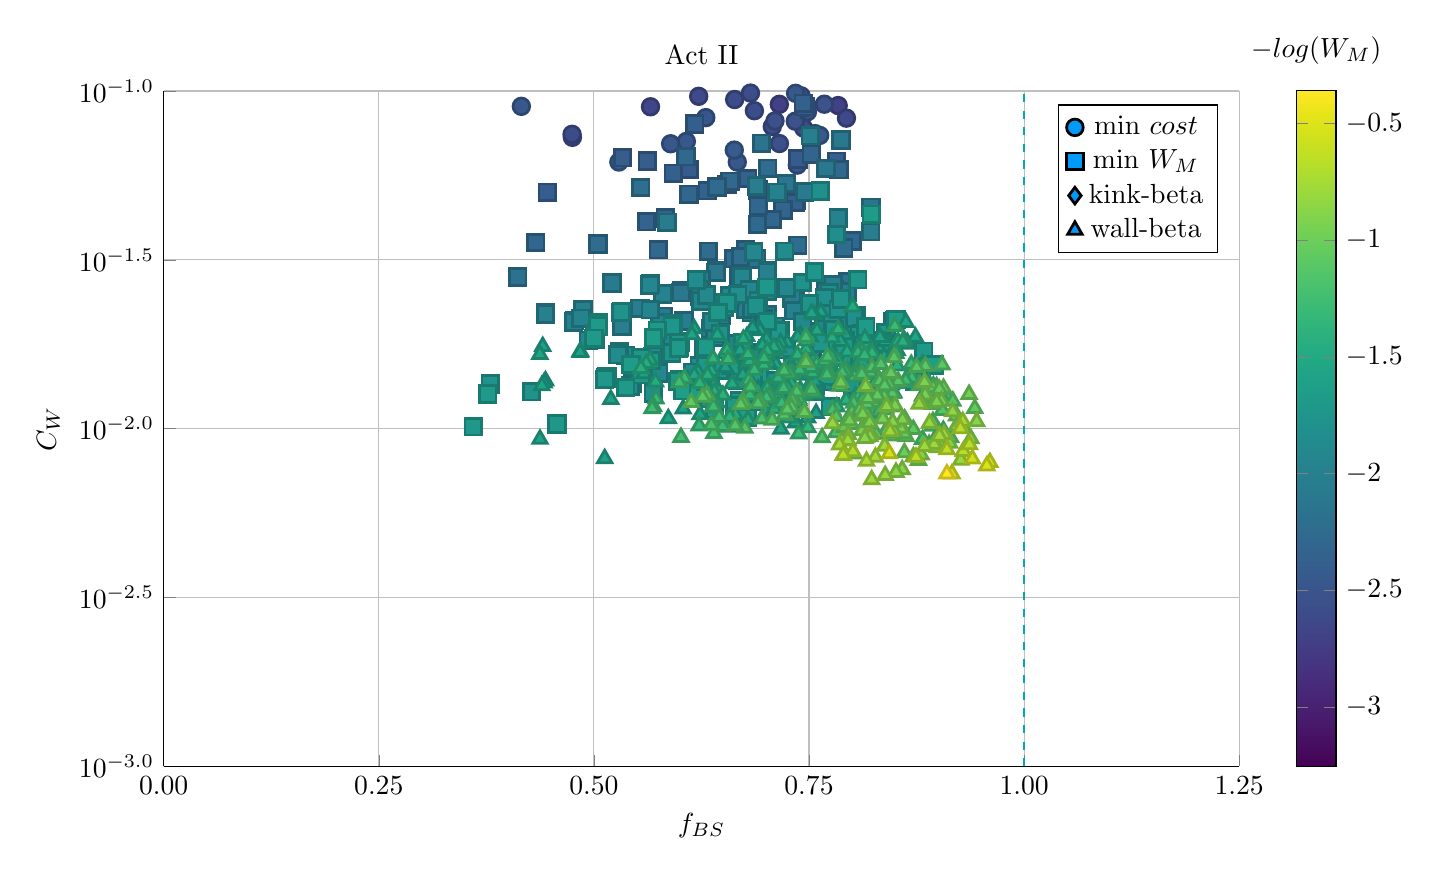
\begin{tikzpicture}[]
\begin{axis}[colorbar = {true}, height = {101.6mm}, ylabel = {${C}_{W}$}, title = {Act II}, xmin = {0.0}, xmax = {1.25}, ymax = {0.1}, ymode = {log}, xlabel = {${f}_{BS}$}, {unbounded coords=jump, scaled x ticks = false, xticklabel style={rotate = 0}, xmajorgrids = true, xtick = {0.0,0.25,0.5,0.75,1.0,1.25}, xticklabels = {0.00,0.25,0.50,0.75,1.00,1.25}, xtick align = inside, axis lines* = left, scaled y ticks = false, yticklabel style={rotate = 0}, log basis y=10, ymajorgrids = true, ytick = {0.001,0.0031622776601683794,0.01,0.03162277660168379,0.1}, yticklabels = {$10^{-3.0}$,$10^{-2.5}$,$10^{-2.0}$,$10^{-1.5}$,$10^{-1.0}$}, ytick align = inside, axis lines* = left,     xshift = 0.0mm,
    yshift = 0.0mm,
    axis background/.style={fill={rgb,1:red,1.00000000;green,1.00000000;blue,1.00000000}}
, colormap={plots}{rgb=(0.26700400,0.00487400,0.32941500), rgb=(0.27794100,0.05632400,0.38119100), rgb=(0.28291000,0.10539300,0.42690200), rgb=(0.28229000,0.14591200,0.46151000), rgb=(0.27619400,0.19007400,0.49300100), rgb=(0.26514500,0.23295600,0.51659900), rgb=(0.25042500,0.27429000,0.53310300), rgb=(0.23360300,0.31382800,0.54391400), rgb=(0.21813000,0.34743200,0.55003800), rgb=(0.20123900,0.38367000,0.55429400), rgb=(0.18555600,0.41857000,0.55675300), rgb=(0.17117600,0.45253000,0.55796500), rgb=(0.15772900,0.48593200,0.55801300), rgb=(0.14618000,0.51541300,0.55682300), rgb=(0.13374300,0.54853500,0.55354100), rgb=(0.12346300,0.58168700,0.54744500), rgb=(0.11948300,0.61481700,0.53769200), rgb=(0.12632600,0.64410700,0.52531100), rgb=(0.15014800,0.67663100,0.50658900), rgb=(0.19109000,0.70836600,0.48228400), rgb=(0.24607000,0.73891000,0.45202400), rgb=(0.31192500,0.76782200,0.41558600), rgb=(0.37777900,0.79178100,0.37793900), rgb=(0.45867400,0.81636300,0.32972700), rgb=(0.54552400,0.83803900,0.27562600), rgb=(0.63690200,0.85654200,0.21662000), rgb=(0.73088900,0.87191600,0.15602900), rgb=(0.81457600,0.88339300,0.11034700), rgb=(0.90631100,0.89485500,0.09812500), rgb=(0.99324800,0.90615700,0.14393600)}, colorbar style={title=$-log( W_M )$}}, ymin = {0.001}, width = {152.4mm}]\addplot+[scatter, scatter src=explicit, only marks = {true}, color = {rgb,1:red,0.00000000;green,0.60560316;blue,0.97868012},
draw opacity=1,
line width=0,
solid,mark = *,
mark size = 3.0,
mark options = {
    color = {rgb,1:red,0.00000000;green,0.00000000;blue,0.00000000}, draw opacity = 1.0,
    fill = {rgb,1:red,0.00000000;green,0.60560316;blue,0.97868012}, fill opacity = 1,
    line width = 1,
    rotate = 0,
    solid
}] coordinates {
(0.7979189762117018, 0.3525334463506062) [-3.255509616138261]
(0.6508511545785957, 0.32947614433956524) [-3.216252832590707]
(0.6207384309764692, 0.3207996295573022) [-3.193009746949994]
(0.7167613746331214, 0.3195481651386946) [-3.177336917116179]
(0.5465767979417996, 0.2581946115377663) [-3.163082372497818]
(0.5529193823663706, 0.2556016866474049) [-3.1626898499465734]
(0.6258847920796543, 0.2803637294509153) [-3.131636779049092]
(0.7917064562365171, 0.251684341414183) [-3.128608643733907]
(0.6571540834017132, 0.2347670840515791) [-3.119490221134428]
(0.7078850901696574, 0.2531440976749766) [-3.109013706519167]
(0.6481638127586685, 0.24990475647251612) [-3.0723306681647147]
(0.6001738293431487, 0.25149441927577304) [-3.052997592637265]
(0.6187389242723457, 0.19130437039826143) [-2.985459255755186]
(0.8495051628857725, 0.18734420194272688) [-2.972314680603446]
(0.7513839499901442, 0.23636228370087514) [-2.944203488565631]
(0.6267065904748437, 0.20245309053686275) [-2.939426129442136]
(0.7241045938835861, 0.20206452850935733) [-2.9330649613663526]
(0.5997525648188614, 0.22794890538650692) [-2.9086175714766993]
(0.7608981275848871, 0.2572349061533023) [-2.883358537184045]
(0.6729097143836795, 0.15434188617247882) [-2.869587308706841]
(0.8757746521895015, 0.16503500153487385) [-2.8642959019839966]
(0.43708561978268146, 0.1540027626199074) [-2.863135499604444]
(0.7737427190330176, 0.1308567738252286) [-2.8571208829882417]
(0.6363044108947997, 0.14971122500360737) [-2.847665218291671]
(0.6336775044410045, 0.16717090103553298) [-2.828598673427815]
(0.6300615768846511, 0.16494453147496302) [-2.828596956391912]
(0.7408717404157776, 0.15144342387609486) [-2.814759126159071]
(0.7973215927503069, 0.1332740186775533) [-2.8111020272923937]
(0.5865353617625098, 0.14502808357996907) [-2.807494730604305]
(0.8920229985384143, 0.18346224251646642) [-2.7988840198100475]
(0.7123981171757686, 0.17577648532919513) [-2.7958756446562494]
(0.8827741971891491, 0.18905695463469122) [-2.7895857162205058]
(0.7770104327826911, 0.15749740379751354) [-2.788746180881234]
(0.6668890153048119, 0.10825265856197185) [-2.7747968746529765]
(0.6418342507827607, 0.11040113988842348) [-2.7708483682382896]
(0.5360832780210509, 0.13338372498410395) [-2.765381217832583]
(0.48591301415870997, 0.1262635120681312) [-2.750591284495743]
(0.8208893899246482, 0.13112338682847605) [-2.7496570559943283]
(0.6826862875440329, 0.15471664525360293) [-2.7416893322109965]
(0.7295311602634156, 0.1412848303800151) [-2.7407501785088124]
(0.7886146632293054, 0.15992855848243978) [-2.7279128729627558]
(0.4222211709016993, 0.10205386518632108) [-2.7258832880958646]
(0.8041946444067724, 0.1537674142036653) [-2.722669285884286]
(0.797307871709929, 0.20286098967446037) [-2.7137612752545364]
(0.7155219569163337, 0.09129627993779868) [-2.7058415620165075]
(0.7839209589323894, 0.09053072224482875) [-2.7028513112666714]
(0.6735514367003905, 0.12001928383918958) [-2.702539859226739]
(0.7781218488522512, 0.1493905369137678) [-2.7023314979575495]
(0.7010648820342178, 0.1037888693016025) [-2.6986339494848854]
(0.7760129209173986, 0.1282449221971978) [-2.6945131020122393]
(0.6990844832209311, 0.1518494521129543) [-2.6791898144381876]
(0.5157995903181049, 0.11667660417497452) [-2.667221125879658]
(0.5823914406465404, 0.10123661778358888) [-2.662660388533524]
(0.5657679431897674, 0.08978187897561334) [-2.6592104485205015]
(0.44749693388894063, 0.13184100351151226) [-2.659078095692512]
(0.5932639482079353, 0.12126631960090636) [-2.65417483710913]
(0.6006546652483065, 0.14162272300343587) [-2.6465645182344044]
(0.5611592944763378, 0.12406919888964466) [-2.6439079819500275]
(0.6911007545926149, 0.11077301491166988) [-2.643696606760721]
(0.7190952149198193, 0.14136171690241212) [-2.640274953402133]
(0.7935005089048651, 0.08309177436606868) [-2.6389176247261594]
(0.7569727025172034, 0.10438808420307069) [-2.6348583782850965]
(0.8024172249496806, 0.15506968293946363) [-2.633251362205558]
(0.8044844370549882, 0.14568324029420993) [-2.628616217379343]
(0.6501793067445676, 0.12693953041669434) [-2.6221141400359933]
(0.7482240633816143, 0.12915735993257627) [-2.6219701923903314]
(0.621764694236391, 0.09641540752157231) [-2.62021595668027]
(0.6592084591590777, 0.12425057651658952) [-2.6147786924049647]
(0.47498517192921386, 0.07289575931420596) [-2.6108221310142987]
(0.4746073853690456, 0.07442364358441783) [-2.605977496081299]
(0.7073486888992542, 0.07847755818800044) [-2.6059699936470437]
(0.6635802472556908, 0.09433825212721927) [-2.5991149525328985]
(0.850954226108881, 0.16713897953620743) [-2.596522935029069]
(0.7438077003960138, 0.0776034126835965) [-2.5952895440733643]
(0.740832976025679, 0.09674674961871782) [-2.585009715337299]
(0.6819729090898469, 0.09857346802331704) [-2.5726509401256643]
(0.686543708388746, 0.08741170684272051) [-2.5725206056757606]
(0.7429105107513022, 0.12936480365836264) [-2.5712497358357154]
(0.6843380338837277, 0.10827230865818141) [-2.564546384231115]
(0.710461808472579, 0.08152119828768783) [-2.5611558991442283]
(0.6762974928856863, 0.1552147025888255) [-2.560527472693454]
(0.715586258869275, 0.06987831618306047) [-2.5592296059708355]
(0.5597844872639409, 0.14085121588272498) [-2.5566843195594604]
(0.7243901373741771, 0.13500017083551635) [-2.5535065866374245]
(0.7280931433532607, 0.12696411777102987) [-2.550740759147308]
(0.6605309873109939, 0.13658873076312603) [-2.5470898857164714]
(0.8355860723725822, 0.11941141738168941) [-2.546206356047881]
(0.7570790485303656, 0.07474738776803291) [-2.5448929680999894]
(0.6786596326251756, 0.10737232651542196) [-2.541474413454408]
(0.7340894798757129, 0.08137452488442802) [-2.537514922795527]
(0.7678322508114538, 0.09136972215165017) [-2.530396423439506]
(0.47114566159008625, 0.1241862768299083) [-2.5150281080837993]
(0.7172945176883795, 0.10923926788923422) [-2.504401804188623]
(0.7481719873715575, 0.08676712224154062) [-2.5023742525367814]
(0.6300392398845994, 0.08338877273150372) [-2.4922625920325645]
(0.6128808203114678, 0.11753681347905565) [-2.487389630851791]
(0.8071640262672946, 0.13435566502497315) [-2.4844945253254624]
(0.7364372722040354, 0.060332641073069196) [-2.4805830368264354]
(0.6074404065469607, 0.07088351332761872) [-2.4785378260843847]
(0.745394573778061, 0.08924008056477738) [-2.472802645920396]
(0.5891419046048868, 0.06977660511757817) [-2.4674178083837037]
(0.5128334577016697, 0.11312298793095699) [-2.466421064277025]
(0.6666521590485631, 0.061573035953788734) [-2.4661166441626214]
(0.41567510391015144, 0.09005659645562718) [-2.462349221395808]
(0.7343893549709765, 0.0984035005548994) [-2.4580995195017694]
(0.7624709680270455, 0.07386191484198576) [-2.452107085174769]
(0.5289955984608532, 0.061603010938046245) [-2.439581368097774]
(0.6631653996596117, 0.0668165076127358) [-2.43556616415459]
};
\addlegendentry{min $cost$}
\addlegendentry{min $W_M$}
\addlegendentry{kink-beta}
\addlegendentry{wall-beta}
\addplot+[scatter, scatter src=explicit, only marks = {true}, color = {rgb,1:red,0.00000000;green,0.60560316;blue,0.97868012},
draw opacity=1,
line width=0,
solid,mark = square*,
mark size = 3.0,
mark options = {
    color = {rgb,1:red,0.00000000;green,0.00000000;blue,0.00000000}, draw opacity = 1.0,
    fill = {rgb,1:red,0.00000000;green,0.60560316;blue,0.97868012}, fill opacity = 1,
    line width = 1,
    rotate = 0,
    solid
}] coordinates {
(0.661464986212126, 0.10974281066537613) [-2.4306307415017843]
(0.7370157733118908, 0.06290604980372316) [-2.424503848137307]
(0.690598661244174, 0.05091548186645167) [-2.420755581201114]
(0.6110332541653926, 0.05858792284393493) [-2.42029590337962]
(0.6501673609257999, 0.11549844358820005) [-2.4141790371623215]
(0.44587667440612394, 0.050141893810974954) [-2.405601237337489]
(0.5620376604250926, 0.06198098521320176) [-2.4024504686412866]
(0.5331847803427727, 0.06341629334440174) [-2.4008644769598204]
(0.74550979710501, 0.08986704512841737) [-2.385303932466634]
(0.6170840429656683, 0.07975071269614381) [-2.3823606631180922]
(0.7351913096719348, 0.0474340690264479) [-2.3815657465744873]
(0.7434927105437699, 0.09186053798374796) [-2.3807722033222922]
(0.6547142049783566, 0.05291391783764062) [-2.379361711103625]
(0.5923718590259175, 0.057089449850007606) [-2.376710844371153]
(0.7339386170283714, 0.04672513349204677) [-2.374327117562279]
(0.7818639646250091, 0.06187465275821013) [-2.3669163111549576]
(0.6786561652806867, 0.05507510194286022) [-2.3631562063698692]
(0.6318904696378785, 0.050697785929454287) [-2.3524541321467844]
(0.7968514952930517, 0.11484809509830482) [-2.344395998367181]
(0.5611693136528799, 0.04103096851706722) [-2.3330913745161674]
(0.7526465794695323, 0.06492210862375562) [-2.3308494031705096]
(0.583020991258734, 0.04209512316597471) [-2.3243681014773663]
(0.719598350762157, 0.0444701106192048) [-2.321057354229076]
(0.7075416069600512, 0.041611663804789) [-2.3099860750527217]
(0.6911305744202555, 0.04576911614498876) [-2.309856205567148]
(0.43244129149250926, 0.03558731274537493) [-2.296581994258459]
(0.6106466677783976, 0.049435012836320257) [-2.2936628719119274]
(0.7849852290380233, 0.05841718863942089) [-2.2871388438649003]
(0.6581369952431696, 0.05397945676504642) [-2.28620876350506]
(0.5748621068441041, 0.03390346024106417) [-2.284352778580142]
(0.6068241978195111, 0.06389678262807066) [-2.275569346907024]
(0.8483848256259394, 0.11453427689842018) [-2.2719687954516363]
(0.8005542007676206, 0.035944140990222695) [-2.270834259062699]
(0.6762652074135871, 0.033926880980726694) [-2.265316297870996]
(0.6430487911671428, 0.052019271065142814) [-2.261664374153362]
(0.690176556067605, 0.040301090484386695) [-2.259848997689232]
(0.6332086139166538, 0.03350083776877989) [-2.2468563010632123]
(0.6624227293490839, 0.031855163498655414) [-2.2457344778364328]
(0.6718053831064826, 0.03090828675529357) [-2.2389914823826476]
(0.5048186250214238, 0.0352012784627346) [-2.2377802921083663]
(0.7019734125243335, 0.05903385354600774) [-2.2342380240743074]
(0.8121176305574418, 0.10969210605285884) [-2.231882297590924]
(0.7903734546200499, 0.034242231307391666) [-2.2294360395026733]
(0.7367663862417018, 0.034924411585111115) [-2.228035836657154]
(0.6704124708860207, 0.032282610822604835) [-2.2174424846206926]
(0.5543099820057378, 0.05175689825632595) [-2.2004811397983373]
(0.6682687098778607, 0.028546322131979412) [-2.185139746320853]
(0.4115404116505872, 0.02810331475808988) [-2.168617871701111]
(0.7950065526437716, 0.0272165314482977) [-2.1647004422479483]
(0.6892985130606427, 0.0317981754636441) [-2.1625687401622105]
(0.694751362041878, 0.06994869676451551) [-2.158758527339496]
(0.7795431083671721, 0.025736452853010065) [-2.1515824844406435]
(0.8218667610241887, 0.04521704877276718) [-2.121990629237416]
(0.7234788593078672, 0.05319946560770676) [-2.120883978806128]
(0.601727381132028, 0.025603626969486912) [-2.1207524337948858]
(0.6423299242995562, 0.029306143991929875) [-2.1201230360983208]
(0.6419300631478283, 0.02906168667526003) [-2.110957023317937]
(0.7504505045074754, 0.022736616298764143) [-2.110380035626549]
(0.6007928001001274, 0.025269195546582173) [-2.1081798456926863]
(0.7697749457010993, 0.05897628607425957) [-2.1067343696105527]
(0.7873060088473159, 0.07161891533416112) [-2.1044579025353145]
(0.6912549105855668, 0.023056958298379608) [-2.101566916256625]
(0.7336421240137444, 0.02613053987073653) [-2.0955802379813457]
(0.7451074741194247, 0.05023579454817505) [-2.084973796814333]
(0.5804505005130721, 0.02151331900190502) [-2.076661850227192]
(0.6242581356920376, 0.027638229223194255) [-2.071490832126067]
(0.6046723929311217, 0.02085479165741199) [-2.069941543407263]
(0.769788121302985, 0.025476612815906984) [-2.0677398411602286]
(0.7635268313674726, 0.022934435495967638) [-2.067409046634433]
(0.5211801885121364, 0.02696996832903912) [-2.064269413912341]
(0.6480874108866086, 0.021601312621323646) [-2.0630315311568608]
(0.6899660212605968, 0.023028993425581536) [-2.0626720924750783]
(0.5850517516052548, 0.04087236955903056) [-2.0538004833692094]
(0.8216243545301457, 0.03829236070332894) [-2.0478939607487705]
(0.7628280730392782, 0.022450092513324634) [-2.0465869927525664]
(0.5324798814823938, 0.020104032121128417) [-2.043557674536744]
(0.6890536830365273, 0.052306726953055445) [-2.0428854364599407]
(0.7788478296863959, 0.02012731448362406) [-2.0423563845025035]
(0.6224577485166921, 0.02464476744428728) [-2.0409243426100203]
(0.7307979150077781, 0.024747950913845577) [-2.040046916152514]
(0.7942304799588185, 0.02537901959969792) [-2.034992533530133]
(0.577461080103995, 0.020640091953131344) [-2.033682476525125]
(0.7779284015524115, 0.026740305901528618) [-2.0310047462120218]
(0.6769291261483851, 0.022560855578882422) [-2.030140567625061]
(0.6353273376932878, 0.019730894484219712) [-2.0274539708881183]
(0.7299639789020798, 0.02440441251419844) [-2.0254028188959325]
(0.5537276388202754, 0.02274030826812891) [-2.0250296365608]
(0.7013111433063811, 0.021697132785661457) [-2.0235785655390583]
(0.5813909087320678, 0.019249263390753116) [-2.0214640585606505]
(0.48743762693577436, 0.02244283453693701) [-2.0200629502616403]
(0.6828397406261851, 0.02203814594228242) [-2.0178425392087607]
(0.4440730615508788, 0.022035211829585857) [-2.0138571764634126]
(0.7515258162028294, 0.07369952986440338) [-2.0135845232118634]
(0.5806654687052556, 0.01907300472793101) [-2.0116905759590398]
(0.6498383055715868, 0.023599926592991906) [-2.010149141557996]
(0.44363452928466746, 0.021831211029723768) [-2.0041930594629993]
(0.7018838410995365, 0.02927306927657322) [-2.0033873272588893]
(0.6972347311275683, 0.021201286808730763) [-2.0011427851405754]
(0.7015769145098381, 0.02913494556354498) [-1.9980234867666669]
(0.6645178610845728, 0.01783938814428187) [-1.9974121702726013]
(0.7321316198336201, 0.02235619021006874) [-1.9950019275945676]
(0.4771771833688903, 0.020886434957250323) [-1.9916414351920695]
(0.6236343599349558, 0.025741017212500165) [-1.990564180292392]
(0.712727225994588, 0.05013311589865279) [-1.9874677312101774]
(0.47652497084149686, 0.020706550326060617) [-1.9837289345498252]
(0.5799439056403491, 0.025041858971509973) [-1.9821147432630368]
(0.6409047748223142, 0.01861582974219078) [-1.9801214965101408]
(0.7541332326057676, 0.01655332174813224) [-1.9749621477739816]
(0.6939183808542294, 0.016797358420123053) [-1.9742296307534244]
(0.5795647235017277, 0.017651648294396863) [-1.9730322510376286]
(0.7841082850109605, 0.042042427337200795) [-1.971389529347601]
(0.6833451595878389, 0.02258381532739581) [-1.9690801869137136]
(0.4846778071403146, 0.021238808369931157) [-1.9626226567046496]
(0.6909628962455928, 0.016548416960404565) [-1.9596270004025225]
(0.5767303440630349, 0.020608512142775547) [-1.958566257945259]
(0.7862802971578733, 0.020599779821979403) [-1.9584820738977198]
(0.7162305112239143, 0.0195177718557608) [-1.954614699115696]
(0.7010347667205691, 0.017040782196874372) [-1.9516708088965276]
(0.6722985157734648, 0.02820222474619141) [-1.9442417891089077]
(0.5656138444137282, 0.02250903467289796) [-1.943873015227273]
(0.565536588821747, 0.026960735925007598) [-1.9427336840285732]
(0.7500685041488271, 0.019332240169876686) [-1.9412579214168701]
(0.7947273212404282, 0.020235695016080246) [-1.9405216947536645]
(0.6805355911014854, 0.025742640357107202) [-1.9325487809339823]
(0.5648058072642934, 0.026603852920062725) [-1.9300873432572263]
(0.8496698518990481, 0.020950775799135048) [-1.9278968643333516]
(0.6579807735398269, 0.024732267535457635) [-1.9276877476527245]
(0.6858091765949128, 0.033391572860488994) [-1.9253231269259206]
(0.5708861139178157, 0.01542840036873154) [-1.9241573414037796]
(0.5910559087252202, 0.01840617725809541) [-1.9233406525196413]
(0.49355969243905806, 0.018260636567552755) [-1.921724789293247]
(0.575157090796294, 0.014637866122214844) [-1.920961736713682]
(0.6934701122157155, 0.01617866914900222) [-1.9187786672199458]
(0.8474953908053612, 0.02070784723390955) [-1.9179865476163513]
(0.7238644822140956, 0.026116835664069596) [-1.9161243062954265]
(0.5363647024122804, 0.016498478570976718) [-1.9143735660644603]
(0.6245725978051111, 0.023866125977571147) [-1.9129187582920881]
(0.7700840154529631, 0.020055932556902554) [-1.9103813974649502]
(0.5018333880946574, 0.018413360294461657) [-1.9088564479888415]
(0.6225054382029354, 0.015368891923046057) [-1.9071998823783851]
(0.6367376179047646, 0.02068382408350092) [-1.9071726014562609]
(0.5295894358084615, 0.016880442428434343) [-1.897974050231251]
(0.6960934824057288, 0.01612411954699371) [-1.8952146302298467]
(0.7426902749138502, 0.02075365260121706) [-1.8938471256212772]
(0.568704237775972, 0.016379710518860197) [-1.8923800441580798]
(0.8036907192437505, 0.014426095962196493) [-1.8897323461694462]
(0.7013203697502467, 0.025505940183094107) [-1.8896025003898504]
(0.5446910677261172, 0.013606302736985727) [-1.8892656634711473]
(0.630889496009857, 0.024905237287315165) [-1.8867582855849152]
(0.6279587919746425, 0.01715148775139446) [-1.882347291055687]
(0.5279648780253892, 0.016558367422903602) [-1.878514829400224]
(0.7105538194684243, 0.02009945768197721) [-1.8778787042091885]
(0.6746951647117155, 0.014479760535701483) [-1.8775947409001372]
(0.542293043100309, 0.01339420829636863) [-1.8732552921128083]
(0.6193122034603253, 0.02767015607394487) [-1.8697993694586394]
(0.7839885834596628, 0.023049355770092206) [-1.8683750435163595]
(0.7216732534757493, 0.033509656125841565) [-1.8677696545788083]
(0.6190250817058932, 0.02748742676505846) [-1.8624097136249032]
(0.5689129347612959, 0.012767822498015982) [-1.8583802932715203]
(0.6151530785874423, 0.014683666893368951) [-1.8574631662150787]
(0.7057769613785234, 0.01751499395644414) [-1.8572895827474112]
(0.6844810134469411, 0.016472273945645852) [-1.8524141700254084]
(0.773635434589481, 0.025198327774631348) [-1.8455171374668375]
(0.792654261453748, 0.013681807567042396) [-1.8385336896572113]
(0.6671435051365248, 0.02496879653899852) [-1.8379981866098642]
(0.5904604397426086, 0.01673941961670631) [-1.8377604849672826]
(0.7666802979827171, 0.02215780908994168) [-1.8334504894389683]
(0.6668097092658632, 0.013870599133405456) [-1.8310127021619171]
(0.7098608245796145, 0.013838791381864052) [-1.8303193689631094]
(0.8054238157512907, 0.021595741757864245) [-1.8289967987219982]
(0.7777188217260086, 0.01376995330170414) [-1.8289040844482014]
(0.781906417020649, 0.03757949039374782) [-1.827554309315621]
(0.6911195041881739, 0.023936582407024766) [-1.8273285755235564]
(0.8048325389616982, 0.021407108284845194) [-1.827200804312974]
(0.7677142381343021, 0.02446003238954006) [-1.8175659191037286]
(0.7152695002223722, 0.019200426003813362) [-1.8168268682337156]
(0.8028502273539799, 0.021283453714909327) [-1.815450986387065]
(0.6836350870936511, 0.012041095014908928) [-1.8126910051980765]
(0.628592104107572, 0.01291346412914029) [-1.8084880440443398]
(0.7631468014994672, 0.050527733393898) [-1.8047994300965564]
(0.7148425638701482, 0.018906858129500544) [-1.8021401154097612]
(0.6470132237632268, 0.01912270586218771) [-1.797704376803326]
(0.5317120643017875, 0.02226583104331943) [-1.7942097853667236]
(0.7424444946037219, 0.027087223311014125) [-1.793491055375234]
(0.6891835376450286, 0.023141087842830272) [-1.7932717403517806]
(0.7770891459148613, 0.020401627221198242) [-1.7894175042201266]
(0.5905174304523498, 0.016723645051687296) [-1.7890530467236028]
(0.5483986928561851, 0.015408130045209871) [-1.7888243529988825]
(0.688859366048084, 0.02301891335039678) [-1.7877136731744465]
(0.5314455106348428, 0.022118529472878953) [-1.7875074347787134]
(0.4274446154942061, 0.012870248723292016) [-1.7837527102877537]
(0.6245047084878231, 0.01260435562894728) [-1.782541611849789]
(0.3796873559941388, 0.013575300034685508) [-1.7790464912523964]
(0.7506208119684119, 0.02342349126521232) [-1.778895445154011]
(0.7233252623099441, 0.017144106473549164) [-1.7714741418782838]
(0.6514218007653796, 0.022914510362698183) [-1.7658936547639612]
(0.8066387483299897, 0.013754397713078726) [-1.764468261837453]
(0.8114336067278799, 0.019143363101630503) [-1.7608302881276638]
(0.7840203897719732, 0.022549750581146864) [-1.758602667193809]
(0.5927329634497353, 0.020422010382537395) [-1.7585010879819967]
(0.6003833781806555, 0.018074242861441603) [-1.756996605404297]
(0.8083920156696353, 0.0189766549148386) [-1.7542805597559368]
(0.6255893892908847, 0.014118662086227647) [-1.7505582033578162]
(0.5988087822527128, 0.017939619250896526) [-1.7500934973153621]
(0.5920216272278206, 0.020256759791424363) [-1.7500334399560231]
(0.7569256367502607, 0.013405307478597901) [-1.7472261906643993]
(0.7874126209259023, 0.02419388957884314) [-1.746682083554902]
(0.8002082164139681, 0.013486675525972136) [-1.746096349326717]
(0.6546258711019086, 0.02357220774846327) [-1.7447580338123476]
(0.5152727776002618, 0.014218446038373668) [-1.744312789986098]
(0.5912172153380305, 0.02010433034226924) [-1.7417418377451568]
(0.7564620723123564, 0.029104896727906955) [-1.7415250046665096]
(0.6457219777667617, 0.014894957040775453) [-1.7412238353155394]
(0.7637505468474293, 0.017939449851622418) [-1.7411299185628226]
(0.5997719558533602, 0.013974274248041367) [-1.738180908045962]
(0.5141931481275667, 0.014117636537660166) [-1.7379493752882689]
(0.6688681240713672, 0.012065781098155766) [-1.7355996958629567]
(0.7794327952990046, 0.019580500348777397) [-1.7326337893718133]
(0.5055186591086885, 0.02066626323270659) [-1.7298549153551994]
(0.6443431702836002, 0.02207237227490677) [-1.7290376820854896]
(0.5124731011428076, 0.013995232804540202) [-1.7282495483556752]
(0.597730217611765, 0.013821785168088184) [-1.727660935507992]
(0.6291789447530073, 0.0136582368693206) [-1.7267105597212837]
(0.45724678194324825, 0.010322088549041144) [-1.725259302096351]
(0.5009956048947217, 0.019077601745993645) [-1.7252009536194264]
(0.8067076340494599, 0.027596176543065832) [-1.7247724234149295]
(0.7144607193282578, 0.0194618140438115) [-1.7238452093782186]
(0.8394015176351165, 0.019251366017915536) [-1.7233992414036838]
(0.566727654847354, 0.01592545730334687) [-1.721095646599682]
(0.7008193261928308, 0.026214129309446717) [-1.7197879690571987]
(0.6301590679475084, 0.015317758062376783) [-1.7194261647044857]
(0.5569499754769649, 0.014599569603833174) [-1.7176951138074539]
(0.5548737682185445, 0.01622912438695158) [-1.7159212174046297]
(0.749938416506126, 0.015548141668362832) [-1.7154343910199206]
(0.805077876563099, 0.016511487187904156) [-1.7152364100930921]
(0.505081072851444, 0.02034931573615192) [-1.7137146048461926]
(0.8832703789161188, 0.01694314067471596) [-1.7130697923553257]
(0.5994765669956786, 0.017414449586085994) [-1.7113330264584932]
(0.8123329425752991, 0.01759386845400357) [-1.711008311762398]
(0.35990367859365535, 0.010137795303924007) [-1.7110001128600978]
(0.7212984156407557, 0.012377995228641003) [-1.7086397826249196]
(0.554696990662245, 0.014458097812438845) [-1.7084719105024766]
(0.6300399549338288, 0.017425831129038206) [-1.7064544131254253]
(0.598355593571199, 0.017308190087748174) [-1.7046060908643599]
(0.3766710822431675, 0.012653057489209665) [-1.7040675703047592]
(0.6638485228747999, 0.0117059662403124) [-1.703202134356769]
(0.7016388084887906, 0.02075998777434103) [-1.7030757309309679]
(0.5735590098298153, 0.019554234789839017) [-1.702622521361834]
(0.504616008782472, 0.020086633015094994) [-1.6997645477508523]
(0.83469594139174, 0.0181903627108964) [-1.696851904940144]
(0.7748772568245458, 0.011615967203161676) [-1.6960415495347418]
(0.6916881185314842, 0.014521159855979892) [-1.6953208270444688]
(0.7986395194652386, 0.016132360346757284) [-1.69504975679679]
(0.5001349243569534, 0.01851904560954049) [-1.6950374418108667]
(0.6402173982163226, 0.011401764722293923) [-1.6889601462509058]
(0.7916321819646072, 0.018187989568727594) [-1.6880264634485147]
(0.5368604078760845, 0.013239606119546703) [-1.6851700918160517]
(0.8159023915755333, 0.020028858328755644) [-1.6835087760477487]
(0.8224969978479914, 0.04313848285475978) [-1.6744813433688244]
(0.6850134649994303, 0.014199586136017074) [-1.6738729070205243]
(0.6732450581236977, 0.017940534735604526) [-1.6717642597891038]
(0.8805571687824683, 0.014044218308111731) [-1.67133201545491]
(0.8510549564630846, 0.021018410614982816) [-1.669280148123924]
(0.6594032075614399, 0.015369545974667817) [-1.6687112321335544]
(0.543104788329551, 0.01549104846164413) [-1.666883215596056]
(0.7829757106136712, 0.01774072617859006) [-1.6662111057335172]
(0.7020803126598293, 0.017288637325639455) [-1.6620335489482105]
(0.8724826946771909, 0.013823569918908126) [-1.6604710222785115]
(0.6032235716053207, 0.012965386105559244) [-1.6601208098191504]
(0.8419078770811601, 0.017125705760294884) [-1.6600202948828224]
(0.6782873077769153, 0.01078451988007799) [-1.6592676966433364]
(0.7322305471022669, 0.015475684627675663) [-1.6587659909376915]
(0.8089032593356332, 0.015516606724815942) [-1.6575006537213521]
(0.8950867510581765, 0.015448369789043721) [-1.6565537181077967]
(0.6213987423559226, 0.012777059141344142) [-1.6557076455143553]
(0.8362668825798195, 0.017802949265934568) [-1.6551218389287718]
(0.7724482845925338, 0.01427965541476533) [-1.6549253512903646]
(0.7561305278900777, 0.012875417406428637) [-1.6533491185988054]
(0.7315646205429555, 0.015371333842334689) [-1.6510880916655832]
(0.6348672268694433, 0.013950721195708211) [-1.6507819655378744]
(0.5692481507228967, 0.018576023932282013) [-1.6487396862283223]
};
\addlegendentry{min $cost$}
\addlegendentry{min $W_M$}
\addlegendentry{kink-beta}
\addlegendentry{wall-beta}
\addplot+[scatter, scatter src=explicit, only marks = {true}, color = {rgb,1:red,0.00000000;green,0.60560316;blue,0.97868012},
draw opacity=1,
line width=0,
solid,mark = diamond*,
mark size = 3.0,
mark options = {
    color = {rgb,1:red,0.00000000;green,0.00000000;blue,0.00000000}, draw opacity = 1.0,
    fill = {rgb,1:red,0.00000000;green,0.60560316;blue,0.97868012}, fill opacity = 1,
    line width = 1,
    rotate = 0,
    solid
}] coordinates {
(0.7185000747593917, 0.01422515042763289) [-1.646438736811751]
};
\addlegendentry{min $cost$}
\addlegendentry{min $W_M$}
\addlegendentry{kink-beta}
\addlegendentry{wall-beta}
\addplot+[scatter, scatter src=explicit, only marks = {true}, color = {rgb,1:red,0.00000000;green,0.60560316;blue,0.97868012},
draw opacity=1,
line width=0,
solid,mark = triangle*,
mark size = 3.0,
mark options = {
    color = {rgb,1:red,0.00000000;green,0.00000000;blue,0.00000000}, draw opacity = 1.0,
    fill = {rgb,1:red,0.00000000;green,0.60560316;blue,0.97868012}, fill opacity = 1,
    line width = 1,
    rotate = 0,
    solid
}] coordinates {
(0.6311197958817455, 0.011957380345402484) [-1.643042565808283]
(0.7582441653604353, 0.011108467862856556) [-1.6423319534513396]
(0.6931064907917183, 0.019535815244331765) [-1.640777244754808]
(0.8300836193269945, 0.017487263260373368) [-1.639221876284111]
(0.6037181675223692, 0.011442088566307322) [-1.6333133834684435]
(0.6872236704168008, 0.01236017109437429) [-1.632965171465297]
(0.7401375444502246, 0.018903756827728994) [-1.6315939840817788]
(0.6844738325068446, 0.019850203149887533) [-1.6312146651728654]
(0.6908969583189651, 0.013104716382950417) [-1.6280817950792132]
(0.44371763261023844, 0.013868549703083988) [-1.6241595906556447]
(0.7574137692390281, 0.01375096435798323) [-1.6236013622276577]
(0.6529161403918602, 0.015182530991955082) [-1.6228047710962017]
(0.7368322785041793, 0.018706655276352954) [-1.6220666148078193]
(0.5580431469661301, 0.014556976982034783) [-1.621952251890808]
(0.7367375521343846, 0.014403289577337152) [-1.6215920184178423]
(0.512526386622637, 0.008161329762295352) [-1.6210091931126354]
(0.6782577239800752, 0.01432854450008374) [-1.618927798748872]
(0.8384377659407821, 0.018146714775031252) [-1.6170623169314409]
(0.48422645670683806, 0.016958271228531874) [-1.616382019877173]
(0.7266472036438298, 0.014563498414899205) [-1.6161622453478632]
(0.6166818733877115, 0.01974854179439184) [-1.6161570213800949]
(0.7247638994629263, 0.017971212251721488) [-1.614542692980794]
(0.44049476009554833, 0.017522649292804678) [-1.6145209017409743]
(0.6292971460452397, 0.013445926670462191) [-1.6116048581596103]
(0.7482933110299739, 0.010771368239357053) [-1.611534614569856]
(0.763658522020206, 0.022148385119972545) [-1.6111378951415813]
(0.7925109151284998, 0.018988318454185676) [-1.610149674607234]
(0.44201361517895554, 0.013672235563415623) [-1.6099909886091608]
(0.48392882775626395, 0.016819394857412875) [-1.6078917791615435]
(0.43733130069402604, 0.009310807818968229) [-1.607743543820338]
(0.864305230174445, 0.01800025118991833) [-1.6036602029724008]
(0.8285261026135398, 0.016454525606269164) [-1.6020241393785943]
(0.7355201630583571, 0.012785938400356595) [-1.5999225299582958]
(0.5196453285989356, 0.012211963891429607) [-1.5991723646523734]
(0.7006220673225357, 0.018397839481491554) [-1.5977458918232372]
(0.7562839792579852, 0.021740628999940625) [-1.5974016193528744]
(0.8620266871415313, 0.01780524184403982) [-1.594452410520862]
(0.7116653004812366, 0.015513011034140182) [-1.593994194232442]
(0.7343913447835282, 0.010444278055928029) [-1.5936858060919608]
(0.6555144127716128, 0.01011718374306493) [-1.591397922325545]
(0.439416009095898, 0.013413579761554176) [-1.5889500828796077]
(0.844780682700243, 0.016637848986608337) [-1.5876067848734392]
(0.6399729359263495, 0.01358109270638293) [-1.5851721171486621]
(0.7791719025737752, 0.016595558848056784) [-1.584524510420682]
(0.7169308474455603, 0.017986619528064067) [-1.5837605102664487]
(0.759653671827968, 0.012669794334412328) [-1.583431339878637]
(0.6796226878396112, 0.01598437293116136) [-1.582579661814279]
(0.6698682770649632, 0.01704223090004215) [-1.58254824230054]
(0.7866687489301921, 0.01813561795940901) [-1.5782874231799235]
(0.6519494273366689, 0.01666388876908953) [-1.5775603382208592]
(0.6810774645893191, 0.012481041135650815) [-1.57691182446182]
(0.6138891419459702, 0.018996299920836554) [-1.576414236089486]
(0.6703307473871568, 0.011717309015560342) [-1.5751504846718982]
(0.8372814378046771, 0.016333627906911542) [-1.5724782812607778]
(0.7766142762619312, 0.016384123578811645) [-1.5724775050016113]
(0.8324306669394973, 0.018651698074430414) [-1.5709179439563137]
(0.6777831213235018, 0.018730631836117465) [-1.5704090936997153]
(0.7530106962183227, 0.021954111137064247) [-1.5702206629127438]
(0.6944921740783251, 0.015799833666457246) [-1.5673098902214302]
(0.5864762498294772, 0.010716322214688368) [-1.565071208714134]
(0.862644544730601, 0.0206551437356325) [-1.5633715250188638]
(0.7002477414970433, 0.011241326563817782) [-1.562850398324037]
(0.6769428405948807, 0.015671331358834917) [-1.5622598064556534]
(0.8737486870967232, 0.01866713656983572) [-1.562193357859922]
(0.845429653689547, 0.013495053157351401) [-1.5609006122749491]
(0.6936663282425067, 0.015665240713829985) [-1.5581504760319127]
(0.437139597354088, 0.016608501930922365) [-1.5581002477100843]
(0.7515605955388661, 0.01869971493207412) [-1.5570326447083804]
(0.6209674005547403, 0.014698104172115228) [-1.5565979804719317]
(0.6730053086177847, 0.014432359414128331) [-1.5554082919617958]
(0.6957698896909281, 0.01765502828342102) [-1.554945197373983]
(0.6233558745289712, 0.01100161562477409) [-1.5547596129791712]
(0.798058696817344, 0.014298720832390546) [-1.5535625342786037]
(0.7306655275003455, 0.013131538889864906) [-1.5534039971370353]
(0.7866695548793657, 0.013546876773104444) [-1.5501529255911566]
(0.7029232410198644, 0.015658705784582727) [-1.549445596593962]
(0.6434881016939706, 0.01896761035049055) [-1.5489435238065508]
(0.8397620904125087, 0.013284856210484001) [-1.5471797462188024]
(0.717359496715404, 0.009969248576619828) [-1.5446347894377386]
(0.7332485919620294, 0.015826339234998477) [-1.541266077478649]
(0.7159117274318698, 0.012014186806033491) [-1.5403018643869486]
(0.7835915318890174, 0.01339409704832976) [-1.5389703051646737]
(0.6166741280693453, 0.01439840233559954) [-1.5350573568418904]
(0.633821998112911, 0.012941961678745326) [-1.5339340799637358]
(0.7591704113820822, 0.019513163303461797) [-1.5312117683334996]
(0.7761504418209141, 0.014559343972861842) [-1.5307460877402002]
(0.6587324098757158, 0.016256389571880216) [-1.5228978664376092]
(0.7301852628673831, 0.015514236909604552) [-1.521832921489891]
(0.6576978830852115, 0.016145546425161975) [-1.515729771633405]
(0.81499015390891, 0.01778179036363044) [-1.513630959409841]
(0.7548783435217022, 0.015911171465456474) [-1.5125041225683304]
(0.7357285740087037, 0.015438155452338993) [-1.5111101431337597]
(0.8914592312756313, 0.013048230181507922) [-1.5092434361014522]
(0.8042266379693425, 0.015165123622893035) [-1.5081635187775795]
(0.7143429209371238, 0.017396326182720072) [-1.5079004665032858]
(0.7106546049776539, 0.01705902254823231) [-1.5062535250464817]
(0.8149595888592437, 0.018516065442475586) [-1.5055927645098854]
(0.6790675991569898, 0.010620725637609863) [-1.5036473207553296]
(0.7263021314438379, 0.01276400588366559) [-1.5023132270207713]
(0.8082959854970523, 0.017501115262627605) [-1.5014348012362577]
(0.644206353529444, 0.012999780153019941) [-1.4991576938374862]
(0.5652726268599519, 0.01595250490442865) [-1.4985359535035265]
(0.7409028369333873, 0.011379775042071525) [-1.4976140962554152]
(0.8525936649214375, 0.017022722224714085) [-1.4966256535092697]
(0.6731323800031858, 0.012123937149914889) [-1.4963366486664067]
(0.794258081171785, 0.016884645135495764) [-1.4932940887021753]
(0.8491221320594042, 0.016877705453300775) [-1.490769198863134]
(0.6606221553518741, 0.013572712784142016) [-1.4903066150781474]
(0.6365115908671835, 0.014812366066278766) [-1.4902753978181227]
(0.698025206737869, 0.011892686690958403) [-1.4902098128895507]
(0.8006325924553926, 0.02294946865378379) [-1.4879353610493]
(0.7312473471464312, 0.0150296355931279) [-1.4839560120603044]
(0.7296317461824722, 0.013588436152737218) [-1.4820439420749398]
(0.6643927224965965, 0.010988676561320621) [-1.4818245705240802]
(0.8818746609117645, 0.015512663790347407) [-1.4812846326350237]
(0.5716681209951134, 0.013758306799242856) [-1.47918844752837]
(0.7019016191748508, 0.016586825363563623) [-1.4784093458682719]
(0.7179877169479433, 0.012454067343383328) [-1.475450492500311]
(0.5608429523532796, 0.015605815957211158) [-1.4747283010824395]
(0.8254737179943745, 0.010706316235513463) [-1.4743446333247474]
(0.7134949866519656, 0.01252952023915475) [-1.4724402875849865]
(0.6386442082590895, 0.012661010708688341) [-1.4715722989768207]
(0.7091780944446543, 0.017420462601206436) [-1.4714857974824802]
(0.7768799795283793, 0.018599806875752512) [-1.4660769216335126]
(0.7138679431480269, 0.011637136699450157) [-1.4647393485582307]
(0.7889526984947632, 0.014453602820187388) [-1.4642398928207598]
(0.7514593158363027, 0.014646400327190036) [-1.4632475994695588]
(0.7483748365137632, 0.013188028157014645) [-1.4627570960518173]
(0.7689030913378709, 0.014992017306240162) [-1.4621262258605858]
(0.9086160751395228, 0.012610442551457213) [-1.4608331013284017]
(0.6736319882181669, 0.018386297428673846) [-1.4592047090200009]
(0.8602710040539581, 0.018375289881343824) [-1.456062319781608]
(0.7158536251686359, 0.013065858856265105) [-1.455536606674486]
(0.6312034180253293, 0.014338289857539464) [-1.4551441312477937]
(0.6842107362565554, 0.016011133350273567) [-1.4550264491991063]
(0.8166413778963588, 0.010490717152993295) [-1.4546079058245875]
(0.8038946210110074, 0.012512538511187441) [-1.4524216104529217]
(0.7253970128236559, 0.013190416768742712) [-1.4512894176116071]
(0.7398530148610076, 0.013058079009232629) [-1.4485556211690722]
(0.8683275099870394, 0.01445380766187149) [-1.4484048810658854]
(0.7757049470190662, 0.01583738294537185) [-1.447827893323938]
(0.6320986387822952, 0.014401012305676196) [-1.4477911002710917]
(0.7095700740504097, 0.011451078951374274) [-1.447547252872805]
(0.8533320108358273, 0.018134028893536453) [-1.447064327609177]
(0.7015808745937036, 0.01701016840471858) [-1.446962882224679]
(0.6809011183945177, 0.015814283798342453) [-1.442801635336501]
(0.7468618453563519, 0.017210162525073) [-1.4427665962214753]
(0.7029265516085115, 0.01341861759657511) [-1.4419746962975288]
(0.7729447381807139, 0.0154167939345581) [-1.4418202869361083]
(0.6401490678816055, 0.012843047050616951) [-1.4414408507394698]
(0.5546511921489885, 0.015092203097265616) [-1.4401670821315686]
(0.8369189847406674, 0.012370078016864275) [-1.4365005858604962]
(0.7271601504533461, 0.010764605563431043) [-1.4362852674891815]
(0.6545941973821089, 0.017113829277376466) [-1.4353336748637542]
(0.83730799707553, 0.01230542875790783) [-1.4335960181347085]
(0.8642748554140802, 0.014217115467473167) [-1.4332076772103557]
(0.8591177437883227, 0.018069625347707154) [-1.4325360351804108]
(0.744692114902789, 0.01254039299533034) [-1.4303317803109008]
(0.7720825896422514, 0.015512017231569421) [-1.427501567848664]
(0.6450976591307117, 0.01041563985641259) [-1.4253033245677857]
(0.7016106537013979, 0.013199067210748885) [-1.424467730606251]
(0.7932422842928847, 0.01214961570743756) [-1.4231002906450272]
(0.8486206904022962, 0.012759691542513012) [-1.4216781469070137]
(0.7651277077779999, 0.015052401942199202) [-1.4189001751593049]
(0.6499004776672259, 0.012568476484747054) [-1.41833361018015]
(0.7468441851636304, 0.018208203061754368) [-1.4162329987544118]
(0.8413757646253268, 0.013515995366956494) [-1.4155721639276562]
(0.8821002961530937, 0.012494038607562102) [-1.4145515245289384]
(0.7371647066538344, 0.012537101480623952) [-1.4108365583003502]
(0.8268385428230587, 0.012002609348078582) [-1.409076294613873]
(0.8524220663316042, 0.015361827479679138) [-1.4090326650511302]
(0.7493488209028417, 0.013020667893253115) [-1.406373031288638]
(0.8369740252258785, 0.013343011801627355) [-1.4049560262744434]
(0.736467741023487, 0.016549665055312992) [-1.4047563528081177]
(0.8437902621307617, 0.01252803721391313) [-1.4043895092023018]
(0.7831971648694067, 0.015932800392846988) [-1.404173626898408]
(0.7760277514230873, 0.016358179284748888) [-1.4023686733295546]
(0.6429968433643665, 0.011931124436664475) [-1.4016206637129285]
(0.7539989813901147, 0.01461149790895501) [-1.397024818172782]
(0.7706190351786399, 0.015159329466703213) [-1.3968614152904222]
(0.7379542397898925, 0.012137377239591915) [-1.3959029594514516]
(0.8198710015233398, 0.016699637953468287) [-1.3916598265412876]
(0.714247100531362, 0.014143727996921667) [-1.3883633874448145]
(0.6578918394886474, 0.010825087435484135) [-1.3880312315362853]
(0.6229039606005311, 0.013613598975867376) [-1.3874617218511183]
(0.7839060606196045, 0.019672506399601233) [-1.3872036434806692]
(0.8945411124249156, 0.013375238696701344) [-1.38697901214861]
(0.8316532620823853, 0.013740114048392838) [-1.3846957819945453]
(0.8105344848695942, 0.01698568487596307) [-1.383828835169896]
(0.678944589993957, 0.016594904366226446) [-1.381775324953039]
(0.8894270189848091, 0.013219706975820847) [-1.3771633347087096]
(0.6384680312659078, 0.016113769323901628) [-1.375512459911651]
(0.8067981871905224, 0.016802690162302802) [-1.3746205580618287]
(0.6378407699069514, 0.012071770627017805) [-1.3743315638371858]
(0.8232503375360749, 0.016757270866106865) [-1.3740148263309282]
(0.8253044011164942, 0.013536984996237456) [-1.3716792526349624]
(0.6377791354466593, 0.011581084185020055) [-1.3700923688132394]
(0.7823161396481406, 0.011606882955578083) [-1.3681667330136331]
(0.6976354608832781, 0.015444033047224012) [-1.3666052322916116]
(0.8256444150010732, 0.011863036441000719) [-1.3649829382620662]
(0.7301576843737896, 0.01456775118335594) [-1.3640705189379334]
(0.7947228629990066, 0.01489280763586952) [-1.3585198589250538]
(0.8852608877000995, 0.012729066389646266) [-1.3565935204567006]
(0.8070688860788532, 0.012400260538805654) [-1.3564751262763801]
(0.8509507442511094, 0.0167128384735583) [-1.351473954153016]
(0.697815302091973, 0.016152303702228896) [-1.3481682159134525]
(0.8322374860885978, 0.011538085240067051) [-1.346993116922072]
(0.812678770383777, 0.011581081741012196) [-1.3435894913269941]
(0.8563585452182935, 0.010097073390939305) [-1.3435331149154779]
(0.7486239762475406, 0.010078781618252586) [-1.3430159394185939]
(0.7586902644694065, 0.015506706786710447) [-1.3398586060696667]
(0.8145940205282202, 0.016490665665914745) [-1.3368201025766182]
(0.8083920408390057, 0.01101776478903974) [-1.3315809886184231]
(0.6865273689258738, 0.014908051955135768) [-1.3309045298779927]
(0.6559187677173682, 0.016046275220657998) [-1.3260036261258312]
(0.8128220992833043, 0.014544434136943774) [-1.3238401611536983]
(0.5721463613293154, 0.012253477656543462) [-1.321256802912694]
(0.75235005778488, 0.015202785039761827) [-1.3206093712463856]
(0.6811784408647148, 0.012588656633960502) [-1.3194256187810434]
(0.88887269591947, 0.013684122702504908) [-1.318071599420516]
(0.8055383651287182, 0.01483503144817611) [-1.3179670437742086]
(0.8369403720951931, 0.012288984556921678) [-1.317828353466683]
(0.7718362914284145, 0.016019467052707494) [-1.3161349019359834]
(0.8228528332017351, 0.011189072959651254) [-1.315933603421898]
(0.6796269178591329, 0.013888279137749418) [-1.3141790233841646]
(0.6222992763725705, 0.010202068294731984) [-1.313144542266674]
(0.7390471882477437, 0.014941236051144027) [-1.3113682925171615]
(0.8038171567694445, 0.014717282341574163) [-1.3109429979139129]
(0.7183921211325701, 0.011910085556243278) [-1.309372125511862]
(0.7684466145126639, 0.015864544513062098) [-1.3071691357120685]
(0.8029734776003514, 0.014248737417105705) [-1.3046977784814981]
(0.7457541419263942, 0.016056591774270774) [-1.3025703125445802]
(0.8422841323050287, 0.013203970264066311) [-1.3005616871122994]
(0.840265556253404, 0.012615186453809279) [-1.3002921900442928]
(0.8303189972786346, 0.012026649703891017) [-1.2988472650706806]
(0.7379824629166711, 0.009652456232370694) [-1.2982796492460857]
(0.8688631987936926, 0.015513448728613892) [-1.2955194103267933]
(0.7553174074604612, 0.012769810565269588) [-1.2945248417209707]
(0.8497311199265203, 0.020110766489847675) [-1.292867454032078]
(0.6051497200603236, 0.014113307404692856) [-1.2908922794934181]
(0.7204536437204339, 0.01317698597914337) [-1.2858788776424053]
(0.7037236784205013, 0.0125261535324546) [-1.2845182494342804]
(0.7276603676026377, 0.014530903531332639) [-1.284181082895186]
(0.8694257292987653, 0.01413859199435929) [-1.2817763493361751]
(0.5693856623324954, 0.011617943765812587) [-1.2788311426055003]
(0.9122738286938411, 0.012303290690253826) [-1.2732310666997158]
(0.8969480471013183, 0.012321239987320123) [-1.272942333188413]
(0.6494823903516777, 0.01015398058126053) [-1.272670278921937]
(0.6388629279464566, 0.011613733735744184) [-1.2718919889201332]
(0.7922783211254797, 0.014799421740279664) [-1.2717012372720022]
(0.7005910682746495, 0.012359217604213728) [-1.2709635745412124]
(0.8623099581829817, 0.013888905579139396) [-1.266888963610956]
(0.5676421853341262, 0.011477750564731057) [-1.2667925209334823]
(0.7884778728955592, 0.014657143187487561) [-1.263414273706133]
(0.8946060241138036, 0.012645106884096416) [-1.2623978734750432]
(0.9061243941401732, 0.009889861997959708) [-1.2609268559147524]
(0.889009728059008, 0.012120958998293596) [-1.2603486826728139]
(0.9023451890438121, 0.01256010485796388) [-1.2603387143491278]
(0.773400562339612, 0.01461415726329041) [-1.2591135123566226]
(0.5991020009858513, 0.01369237968282258) [-1.2586437273293951]
(0.8899703330660784, 0.012541527523495959) [-1.257653219851325]
(0.7376230224097893, 0.012286926968559252) [-1.2561210915813497]
(0.8517469553571062, 0.0136337642943094) [-1.255368451886125]
(0.8310600091864557, 0.01121214505467198) [-1.2548793145438668]
(0.7463767079119895, 0.018674483010578485) [-1.2512638217028496]
(0.9010953161455407, 0.00977433077244536) [-1.2508797544185108]
(0.7708084845070091, 0.01445226067935465) [-1.2483881975700346]
(0.8255911895303738, 0.014810410864156564) [-1.2472111495180525]
(0.6456889630234938, 0.010801319399384545) [-1.2461997489620957]
(0.7211206255852547, 0.014822874842934698) [-1.2418625029140806]
(0.8212435765459043, 0.01465291764892327) [-1.2379995353756044]
(0.8124106215521333, 0.012184198873488754) [-1.237493864731498]
(0.7773617952030372, 0.011365478091521037) [-1.234135730311014]
(0.6012269905062186, 0.00943024217488651) [-1.2290480585366261]
(0.6822646003191638, 0.013294538688928005) [-1.226535075176338]
(0.7715760698999713, 0.016313912238560754) [-1.2245765023063588]
(0.6394599559527891, 0.009692623044267795) [-1.2205912294761325]
(0.8778575910479186, 0.013424043119551074) [-1.2202282901047126]
(0.8019239914949399, 0.011910043296521748) [-1.2162624283663717]
(0.6952679442175284, 0.010687666973582014) [-1.216086509297852]
(0.7317625637140489, 0.012330739546211958) [-1.21390928237209]
(0.842755408696742, 0.01215930137847683) [-1.2049966301404438]
(0.8389669084464072, 0.01150325833203817) [-1.2028519625289822]
(0.7530473416398337, 0.013035397004774626) [-1.2017262807398885]
(0.8820785476236526, 0.009301145332038834) [-1.2014767991416744]
(0.8343149074377907, 0.012419137314354196) [-1.1974933870834255]
(0.7357075286074418, 0.012866951754200074) [-1.1902268010386523]
(0.6363750412326489, 0.010250374516218385) [-1.1897384323587963]
(0.8393687651664384, 0.01265322941070475) [-1.184690201740547]
(0.69353160604751, 0.012043129558995997) [-1.1824787036075495]
(0.7813811749481642, 0.009737455861362002) [-1.1808858550280483]
(0.82312990693351, 0.015201335495023468) [-1.1781326616624272]
(0.8230125850446273, 0.012111892614755496) [-1.1777544033937284]
(0.8113330722036027, 0.014497113124643852) [-1.1767713500639074]
(0.8151433740010974, 0.011360692844488932) [-1.1763851472141231]
(0.7212726504485895, 0.010993209125132675) [-1.1710046722732435]
(0.6906836593755131, 0.011873108025089065) [-1.168064001469266]
(0.8335582258475951, 0.01551684893294213) [-1.1641390547368031]
(0.8397877730881088, 0.014435683021864657) [-1.1590154051437593]
(0.8077889232819103, 0.011133219242928594) [-1.156719055806647]
(0.8457004982517811, 0.011598274765611892) [-1.153859959499507]
(0.7997486547078345, 0.011195300959476255) [-1.1511509149367658]
(0.6754638865508275, 0.010035803760267933) [-1.1483727579139014]
(0.7651889142799113, 0.0094080192606344) [-1.147105832517893]
(0.8245678050026981, 0.011995225527156074) [-1.1453947736271883]
(0.7859979698894712, 0.013365277618352068) [-1.1452404623261505]
(0.893299490957302, 0.010186035899141098) [-1.1451816190996513]
(0.9050526879154615, 0.011334530949821734) [-1.1446532223243113]
(0.6642394260086819, 0.01021123269482473) [-1.1400919625251364]
(0.672416445613222, 0.01195592909100127) [-1.1390956800435426]
(0.8469029397972263, 0.012735988750448667) [-1.1386372425544071]
(0.8378925522661699, 0.011373713628310371) [-1.1358940070608368]
(0.8390207981736643, 0.00982386795341639) [-1.135681514185642]
(0.7072454567231232, 0.010610674356319873) [-1.135165267470295]
(0.8537078011785187, 0.013810994201479724) [-1.1332899010842914]
(0.8176502578366862, 0.011837559393240335) [-1.13313920209278]
(0.7303730036989917, 0.012096251950497844) [-1.1307498874595736]
(0.894013996908693, 0.010497513784941466) [-1.127968963904733]
(0.7816453004288693, 0.010834008197391748) [-1.12386756745346]
(0.8374212130377817, 0.012467361173172) [-1.1215587926222255]
(0.8427999604173193, 0.013535996445327877) [-1.121496864445471]
(0.8282914956410142, 0.009646722759962213) [-1.120489276300089]
(0.7297691603664651, 0.011569661309773186) [-1.1184055953309242]
(0.8320705165048677, 0.013807513435897366) [-1.1181592404462695]
(0.8896163477116564, 0.00899022314859978) [-1.11727638544861]
(0.8488615529169612, 0.016244323813180382) [-1.1157863931853709]
(0.917135410698358, 0.012075661203497881) [-1.1152893394825385]
(0.8379419053360844, 0.013415311693851309) [-1.1147254655918233]
(0.6312043050337759, 0.01260299051150895) [-1.1110721919268842]
(0.8983105025174212, 0.01332771142026984) [-1.110900623566253]
(0.885351265072503, 0.015330361242962491) [-1.1102178959125066]
(0.8087211722311475, 0.011352559077866435) [-1.1065637050760246]
(0.8943370090651046, 0.01322563487331611) [-1.1055185111305836]
(0.9047382401512668, 0.015443585785573642) [-1.104513956272333]
(0.7246235014150954, 0.011397535860200515) [-1.1032817598575653]
(0.8750741551870631, 0.015180088195150168) [-1.102413872968577]
(0.8790731029814186, 0.0134320665083267) [-1.0976081941747866]
(0.6262877505019419, 0.012410135763042724) [-1.0960422057486803]
(0.74647209508259, 0.015710188085172192) [-1.0908223470837244]
(0.9145445175929484, 0.009416494887639834) [-1.0901798613450124]
(0.6739379291616313, 0.011950330291897161) [-1.0895239334380136]
(0.798713588111754, 0.010302183604603485) [-1.0819707722700944]
(0.6705941774315217, 0.011781112313774076) [-1.074757862571252]
(0.8712568609040067, 0.009953672306844926) [-1.0646247705781775]
(0.8293776375253815, 0.012529471726161237) [-1.061634359556082]
(0.7905572156565129, 0.010083847832352364) [-1.0600956611746053]
(0.8593725840136144, 0.009928133893917744) [-1.0596254236181546]
(0.6129308097183813, 0.011966322509718732) [-1.057368504037735]
(0.8573442630715564, 0.009681667371421088) [-1.0565554871926919]
(0.8611676740206385, 0.010691691035459546) [-1.0537891320708912]
(0.9426739289422088, 0.011486077050440274) [-1.04986917283876]
(0.8185235390136167, 0.012292882091147163) [-1.0455609247586943]
(0.8460752873247276, 0.009530561897370601) [-1.0452172255175898]
(0.8482858666033886, 0.009729002321664978) [-1.0428358674069769]
(0.8451724979224685, 0.014575387501866556) [-1.039901763406582]
(0.8628054828549602, 0.00947356502622826) [-1.0389907356074144]
(0.8608227332547408, 0.009674610417963237) [-1.0385143992937391]
(0.8931149172988149, 0.011807111154597752) [-1.0342806593516065]
(0.7446465532782998, 0.011176208487319431) [-1.0342733550292629]
(0.9063469500741413, 0.013180443572509375) [-1.0277452020904507]
(0.9015425066983972, 0.013079381492890091) [-1.0231184927600263]
(0.8868548323368646, 0.012467541057991872) [-1.014480859446761]
(0.7869791979733861, 0.01369139591582246) [-1.0143022984006733]
(0.8133076369841958, 0.010906621011059782) [-1.0119941373404269]
(0.8608478207457898, 0.008491096978099041) [-1.0018416320745183]
(0.9215695881050738, 0.010922748298841226) [-0.9929535525024817]
(0.8025151408671897, 0.00841789073748284) [-0.9894291146448607]
(0.9360622329224974, 0.012640368074675423) [-0.9863753440678572]
(0.7971178835760543, 0.010560312689328725) [-0.984748777374235]
(0.8772406259344445, 0.008060111656535808) [-0.9828312076920769]
(0.8124276875467605, 0.011043921456953326) [-0.9671614250059299]
(0.9302857302897223, 0.010049939978986342) [-0.9588341781257976]
(0.8849557090540082, 0.012587255211307845) [-0.9559077487615911]
(0.8357770277720186, 0.010692244192616846) [-0.9550279719211583]
(0.9020594673841236, 0.009394203027706034) [-0.9530739329383017]
(0.8812729705330123, 0.011875902168419222) [-0.9523094842842953]
(0.9041870110761893, 0.00886218364662139) [-0.9443733077337034]
(0.8500366352517474, 0.011692840854153322) [-0.9389066887263714]
(0.9039162498590035, 0.012088768216592539) [-0.938718731273603]
(0.8116200312519593, 0.009873846925000044) [-0.9368220763401279]
(0.8983774109908026, 0.011985445552666077) [-0.9338499055050675]
(0.820464847854049, 0.010417116602885905) [-0.9320199493225862]
(0.8843133057410291, 0.013724205308149058) [-0.9299360593988208]
(0.8563674650178192, 0.010039835769091158) [-0.9254830601542069]
(0.8586449265826853, 0.010632326673406257) [-0.9177947234167438]
(0.7955837503816072, 0.009618156275270644) [-0.9110248491185311]
(0.9216137886121949, 0.010202468666222132) [-0.910255608760031]
(0.8485781402839475, 0.009862813893055277) [-0.9087309290200033]
(0.8226633013231592, 0.009617356766200968) [-0.9071167674774879]
(0.8472170390833825, 0.010459816469032294) [-0.9069228085429362]
(0.8158631361456505, 0.013336941021222104) [-0.9012193459269542]
(0.7881487533500626, 0.009211323142223135) [-0.8955780050272362]
(0.9381999951129822, 0.009343910498799778) [-0.8933161335121345]
(0.8803401921411356, 0.008372851970004534) [-0.8930419732360771]
(0.9133927793035722, 0.00907072512178995) [-0.8918346519545955]
(0.9067663787137008, 0.009623400857030357) [-0.89144729138945]
(0.816256836915202, 0.009443043533545779) [-0.888899846836759]
(0.8208847736701266, 0.009473962015038109) [-0.8855085355474239]
(0.8713135819539694, 0.008266202480666536) [-0.8847739413810434]
(0.840183845958757, 0.011644648814523576) [-0.8844033061643041]
(0.8582829008420433, 0.007565406000956704) [-0.8757064563443095]
(0.8148734133865592, 0.009364903942846628) [-0.8752130243312761]
(0.9447921539123566, 0.010497601675246136) [-0.8735123104376383]
(0.8510933760061492, 0.007432232654899479) [-0.857777575430145]
(0.9169530110018537, 0.01122792294531789) [-0.8521104842000996]
(0.7771638249759684, 0.010360618428916071) [-0.8317136706966171]
(0.8780027063131941, 0.011829183524206692) [-0.8282322662317392]
(0.8900989858251497, 0.010386187143878832) [-0.8236382617419924]
(0.8385657406662046, 0.007274304586793455) [-0.8182707043090822]
(0.8994170598745475, 0.008796601702267225) [-0.816574798417258]
(0.9264691512067383, 0.008077559702919766) [-0.8017991777009724]
(0.8953674722871903, 0.008984149049243224) [-0.7963475526884611]
(0.8228638598364941, 0.007065713081305555) [-0.792512235520203]
(0.8843519513605289, 0.008863210685214288) [-0.7886491137533254]
(0.9068434829587347, 0.009614384932251367) [-0.7859589112061925]
(0.8441936870918764, 0.009803091719826367) [-0.7855587468920852]
(0.795195330186583, 0.009233251065538626) [-0.7846782722559245]
(0.8379259727633699, 0.008882362960772126) [-0.7789165425502128]
(0.9015492919799136, 0.009511474877739953) [-0.7767397769810044]
(0.827186368518997, 0.008236835640706432) [-0.7659728569178655]
(0.9286980581689553, 0.010513825095306002) [-0.7612366628570103]
(0.7855196102124484, 0.008951530949801032) [-0.7509876539770305]
(0.8168180745109146, 0.008011940841449515) [-0.7391271780145358]
(0.8010536666905443, 0.00855489391676945) [-0.7054527932453033]
(0.9259588799167481, 0.010008848514648037) [-0.6848908242429158]
(0.7897320855863864, 0.00834551568243046) [-0.6812678712644065]
(0.9292483679059809, 0.008576192775533141) [-0.6756061545310171]
(0.8743266272501374, 0.008241144070801919) [-0.6739602998385263]
(0.9365046535466279, 0.00897130340792402) [-0.6642851794810503]
(0.910279153280067, 0.008668304282515152) [-0.6535759824011087]
(0.9602367452182844, 0.007951334012599445) [-0.5746045676839148]
(0.9161618961363623, 0.0073565768554252) [-0.5618173228824405]
(0.9398958911545593, 0.008137722391679258) [-0.5591823521052834]
(0.8433586013356281, 0.00843813948044561) [-0.5508144644637797]
(0.9566973138966702, 0.007769849764460444) [-0.5201034007347762]
(0.9102893107680471, 0.007355361549158748) [-0.3603172686032916]
};
\addlegendentry{min $cost$}
\addlegendentry{min $W_M$}
\addlegendentry{kink-beta}
\addlegendentry{wall-beta}
\addplot+ [color = {rgb,1:red,0.00000048;green,0.66575898;blue,0.68099695},
draw opacity=1.0,
line width=1,
dashed,mark = none,
mark size = 2.0,
mark options = {
    color = {rgb,1:red,0.00000000;green,0.00000000;blue,0.00000000}, draw opacity = 1.0,
    fill = {rgb,1:red,0.00000048;green,0.66575898;blue,0.68099695}, fill opacity = 1.0,
    line width = 1,
    rotate = 0,
    solid
},forget plot]coordinates {
(1.0, 0.001)
(1.0, 0.1)
};
\end{axis}

\end{tikzpicture}

		\end{adjustbox}
        \caption{Act II $l_i$ Sampling}
    \end{subfigure}	
    \hfill \hfill ~\\ ~\\ ~\\
    \caption{Bootstrap Current Monte Carlo Sampling}
    \label{fig:bootstrap_samplings}
\end{figure*}

The next plot is the parameter that determines a current profile's peak radius: $l_i$. As can be seen, the current peak approaches the outer edge of the plasma as $l_i$ decreases. This in turn boosts the bootstrap fraction closer to one -- leading to inexpensive reactors.

\begin{figure*}
    \centering
    \hfill 
    \begin{subfigure}[t]{0.45\textwidth}
        \centering
		\begin{adjustbox}{width=\textwidth}
			\Large
			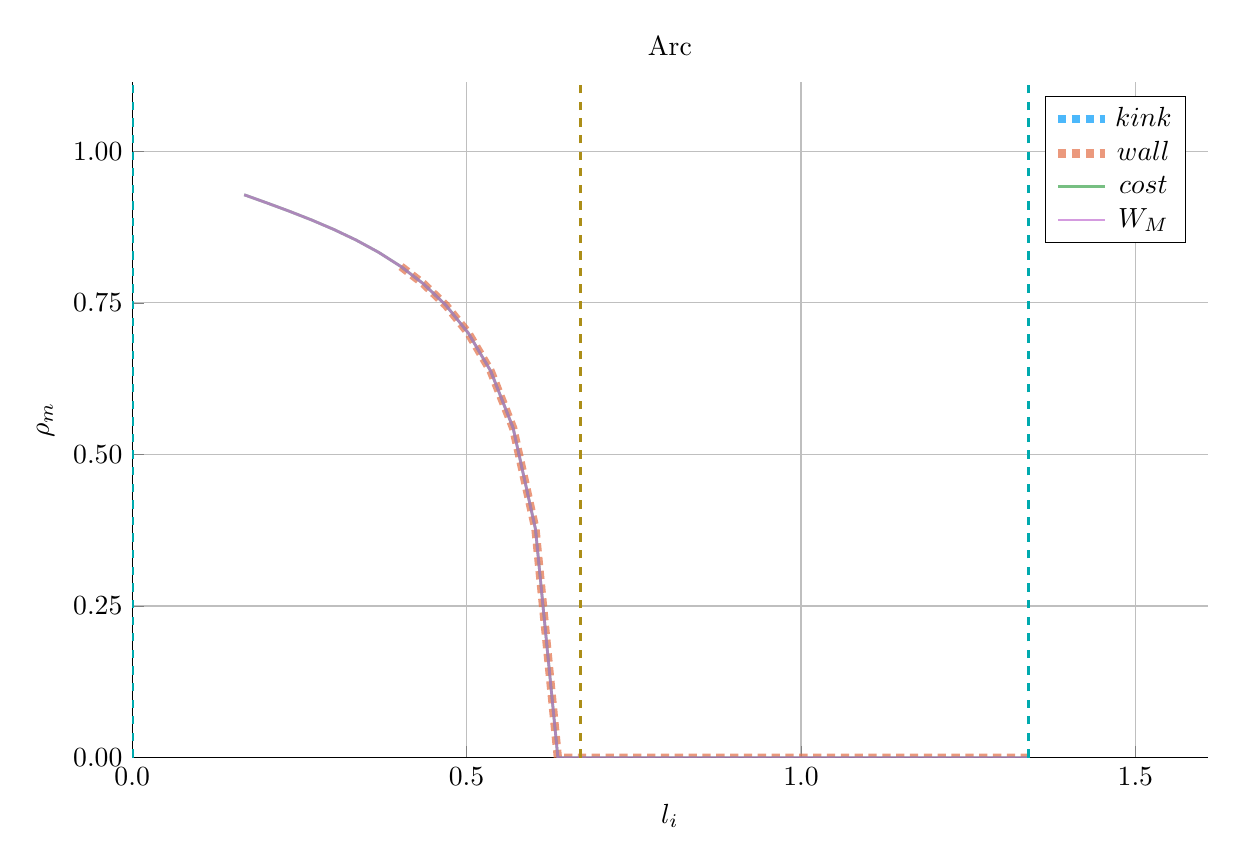
\begin{tikzpicture}[]
\begin{axis}[height = {101.6mm}, ylabel = {${\rho}_{m}$}, title = {Arc}, xmin = {0.0}, xmax = {1.608}, ymax = {1.1138397976901306}, xlabel = {${l}_{i}$}, {unbounded coords=jump, scaled x ticks = false, xticklabel style={rotate = 0}, xmajorgrids = true, xtick = {0.0,0.5,1.0,1.5}, xticklabels = {0.0,0.5,1.0,1.5}, xtick align = inside, axis lines* = left, scaled y ticks = false, yticklabel style={rotate = 0}, ymajorgrids = true, ytick = {0.0,0.25,0.5,0.75,1.0}, yticklabels = {0.00,0.25,0.50,0.75,1.00}, ytick align = inside, axis lines* = left,     xshift = 0.0mm,
    yshift = 0.0mm,
    axis background/.style={fill={rgb,1:red,1.00000000;green,1.00000000;blue,1.00000000}}
, colorbar style={title=}}, ymin = {0.0}, width = {152.4mm}]\addplot+ [color = {rgb,1:red,0.00000000;green,0.60560316;blue,0.97868012},
draw opacity=0.7,
line width=3,
dotted,mark = none,
mark size = 2.0,
mark options = {
    color = {rgb,1:red,0.00000000;green,0.00000000;blue,0.00000000}, draw opacity = 0.7,
    fill = {rgb,1:red,0.00000000;green,0.60560316;blue,0.97868012}, fill opacity = 0.7,
    line width = 1,
    rotate = 0,
    solid
}]coordinates {
(0.2345, 0.9012554395329321)
};
\addlegendentry{$kink$}
\addplot+ [color = {rgb,1:red,0.88887350;green,0.43564919;blue,0.27812294},
draw opacity=0.7,
line width=3,
dotted,mark = none,
mark size = 2.0,
mark options = {
    color = {rgb,1:red,0.00000000;green,0.00000000;blue,0.00000000}, draw opacity = 0.7,
    fill = {rgb,1:red,0.88887350;green,0.43564919;blue,0.27812294}, fill opacity = 0.7,
    line width = 1,
    rotate = 0,
    solid
}]coordinates {
(0.402, 0.8097578932696892)
(0.4355, 0.7813881988360357)
(0.469, 0.7460807709758508)
(0.5025, 0.7003128400554752)
(0.536, 0.6375996141396295)
(0.5695, 0.5439347841396138)
(0.603, 0.3769651924898696)
(0.6365, 0.0)
(0.67, 0.0)
(0.7035, 0.0)
(0.737, 0.0)
(0.804, 0.0)
(0.8375, 0.0)
(0.871, 0.0)
(0.9045, 0.0)
(0.938, 0.0)
(0.9715, 0.0)
(1.005, 0.0)
(1.0385, 0.0)
(1.072, 0.0)
(1.1055, 0.0)
(1.139, 0.0)
(1.1725, 0.0)
(1.206, 0.0)
(1.2395, 0.0)
(1.273, 0.0)
(1.3065, 0.0)
(1.34, 0.0)
};
\addlegendentry{$wall$}
\addplot+ [color = {rgb,1:red,0.24222430;green,0.64327509;blue,0.30444865},
draw opacity=0.7,
line width=1,
solid,mark = none,
mark size = 2.0,
mark options = {
    color = {rgb,1:red,0.00000000;green,0.00000000;blue,0.00000000}, draw opacity = 0.7,
    fill = {rgb,1:red,0.24222430;green,0.64327509;blue,0.30444865}, fill opacity = 0.7,
    line width = 1,
    rotate = 0,
    solid
}]coordinates {
(0.1675, 0.9281998314084423)
(0.201, 0.9149279593755997)
(0.2345, 0.9012554395329321)
(0.268, 0.8867623689514805)
(0.3015, 0.8709916945680435)
(0.335, 0.8534031690137241)
(0.3685, 0.83330636296198)
(0.402, 0.8097578932696893)
(0.4355, 0.7813881988360357)
(0.469, 0.7460807709758508)
(0.5025, 0.7003128400554761)
(0.536, 0.6375996141396301)
(0.5695, 0.5439347841396126)
(0.603, 0.3769651924898652)
(0.6365, 0.0)
(0.67, 0.0)
(0.7035, 0.0)
(0.737, 0.0)
(0.804, 0.0)
(0.8375, 0.0)
(0.871, 0.0)
(0.9045, 0.0)
(0.938, 0.0)
(0.9715, 0.0)
(1.005, 0.0)
(1.0385, 0.0)
(1.072, 0.0)
(1.1055, 0.0)
(1.139, 0.0)
(1.1725, 0.0)
(1.206, 0.0)
(1.2395, 0.0)
(1.273, 0.0)
(1.3065, 0.0)
(1.34, 0.0)
};
\addlegendentry{$cost$}
\addplot+ [color = {rgb,1:red,0.76444018;green,0.44411178;blue,0.82429754},
draw opacity=0.7,
line width=1,
solid,mark = none,
mark size = 2.0,
mark options = {
    color = {rgb,1:red,0.00000000;green,0.00000000;blue,0.00000000}, draw opacity = 0.7,
    fill = {rgb,1:red,0.76444018;green,0.44411178;blue,0.82429754}, fill opacity = 0.7,
    line width = 1,
    rotate = 0,
    solid
}]coordinates {
(0.1675, 0.9281998314084423)
(0.201, 0.9149279593755996)
(0.2345, 0.9012554395329321)
(0.268, 0.8867623689514806)
(0.3015, 0.8709916945680435)
(0.335, 0.8534031690137243)
(0.3685, 0.8333063629619801)
(0.402, 0.8097578932696893)
(0.4355, 0.7813881988360356)
(0.469, 0.7460807709758505)
(0.5025, 0.7003128400554756)
(0.536, 0.6375996141396283)
(0.5695, 0.5439347841396114)
(0.603, 0.3769651924898696)
(0.6365, 0.0)
(0.67, 0.0)
(0.7035, 0.0)
(0.737, 0.0)
(0.804, 0.0)
(0.8375, 0.0)
(0.871, 0.0)
(0.9045, 0.0)
(0.938, 0.0)
(0.9715, 0.0)
(1.005, 0.0)
(1.0385, 0.0)
(1.072, 0.0)
(1.1055, 0.0)
(1.139, 0.0)
(1.1725, 0.0)
(1.206, 0.0)
(1.2395, 0.0)
(1.273, 0.0)
(1.3065, 0.0)
(1.34, 0.0)
};
\addlegendentry{$W_M$}
\addplot+ [color = {rgb,1:red,0.67554396;green,0.55566233;blue,0.09423434},
draw opacity=1.0,
line width=1,
dashed,mark = none,
mark size = 2.0,
mark options = {
    color = {rgb,1:red,0.00000000;green,0.00000000;blue,0.00000000}, draw opacity = 1.0,
    fill = {rgb,1:red,0.67554396;green,0.55566233;blue,0.09423434}, fill opacity = 1.0,
    line width = 1,
    rotate = 0,
    solid
},forget plot]coordinates {
(0.67, 0.0)
(0.67, 1.1138397976901306)
};
\addplot+ [color = {rgb,1:red,0.00000048;green,0.66575898;blue,0.68099695},
draw opacity=1.0,
line width=1,
dashed,mark = none,
mark size = 2.0,
mark options = {
    color = {rgb,1:red,0.00000000;green,0.00000000;blue,0.00000000}, draw opacity = 1.0,
    fill = {rgb,1:red,0.00000048;green,0.66575898;blue,0.68099695}, fill opacity = 1.0,
    line width = 1,
    rotate = 0,
    solid
},forget plot]coordinates {
(0.0, 0.0)
(0.0, 1.1138397976901306)
};
\addplot+ [color = {rgb,1:red,0.00000048;green,0.66575898;blue,0.68099695},
draw opacity=1.0,
line width=1,
dashed,mark = none,
mark size = 2.0,
mark options = {
    color = {rgb,1:red,0.00000000;green,0.00000000;blue,0.00000000}, draw opacity = 1.0,
    fill = {rgb,1:red,0.00000048;green,0.66575898;blue,0.68099695}, fill opacity = 1.0,
    line width = 1,
    rotate = 0,
    solid
},forget plot]coordinates {
(1.34, 0.0)
(1.34, 1.1138397976901306)
};
\end{axis}

\end{tikzpicture}

		\end{adjustbox}
        \caption{Arc Peak Radius}
    \end{subfigure}
    \hfill
    \begin{subfigure}[t]{0.45\textwidth}
        \centering
		\begin{adjustbox}{width=\textwidth}
			\Large
			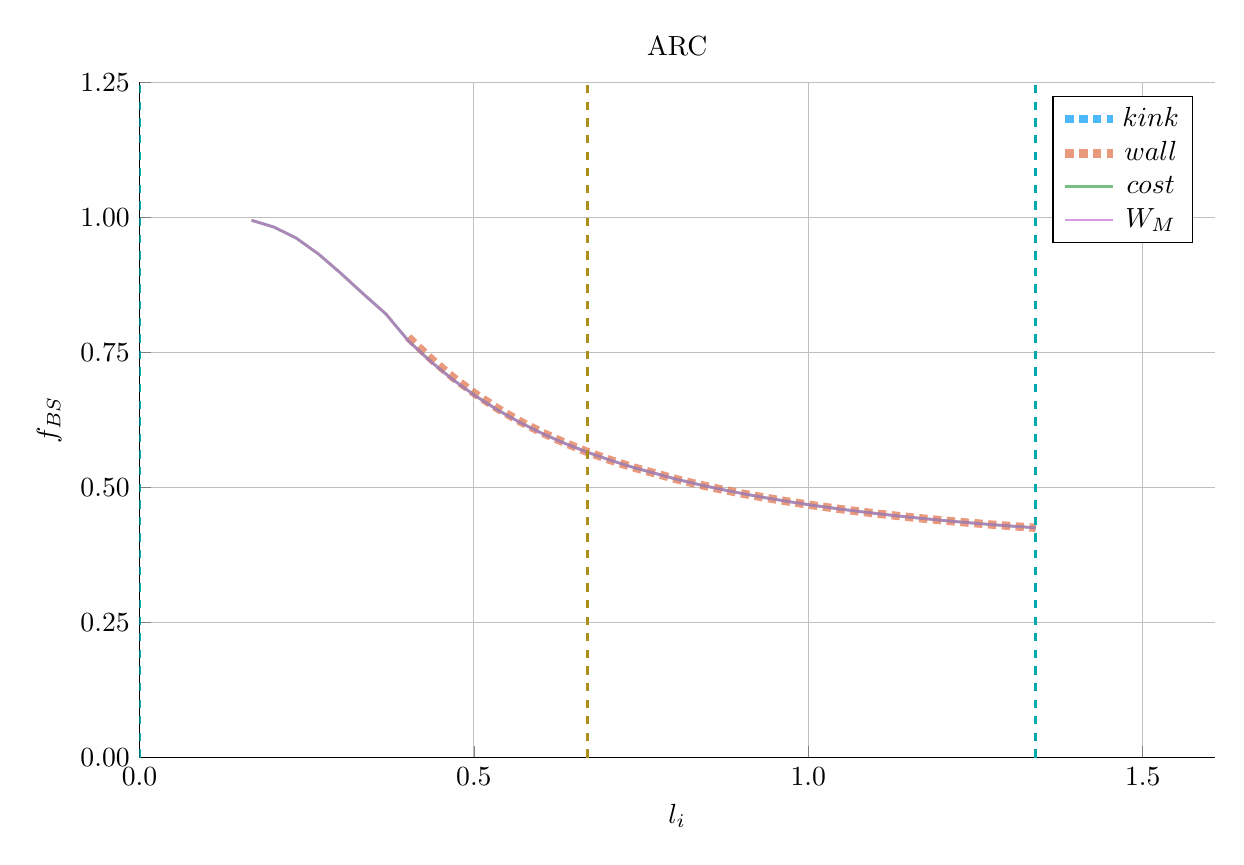
\begin{tikzpicture}[]
\begin{axis}[height = {101.6mm}, ylabel = {${f}_{BS}$}, title = {ARC}, xmin = {0.0}, xmax = {1.608}, ymax = {1.25}, xlabel = {${l}_{i}$}, {unbounded coords=jump, scaled x ticks = false, xticklabel style={rotate = 0}, xmajorgrids = true, xtick = {0.0,0.5,1.0,1.5}, xticklabels = {0.0,0.5,1.0,1.5}, xtick align = inside, axis lines* = left, scaled y ticks = false, yticklabel style={rotate = 0}, ymajorgrids = true, ytick = {0.0,0.25,0.5,0.75,1.0,1.25}, yticklabels = {0.00,0.25,0.50,0.75,1.00,1.25}, ytick align = inside, axis lines* = left,     xshift = 0.0mm,
    yshift = 0.0mm,
    axis background/.style={fill={rgb,1:red,1.00000000;green,1.00000000;blue,1.00000000}}
, colorbar style={title=}}, ymin = {0.0}, width = {152.4mm}]\addplot+ [color = {rgb,1:red,0.00000000;green,0.60560316;blue,0.97868012},
draw opacity=0.7,
line width=3,
dotted,mark = none,
mark size = 2.0,
mark options = {
    color = {rgb,1:red,0.00000000;green,0.00000000;blue,0.00000000}, draw opacity = 0.7,
    fill = {rgb,1:red,0.00000000;green,0.60560316;blue,0.97868012}, fill opacity = 0.7,
    line width = 1,
    rotate = 0,
    solid
}]coordinates {
(0.2345, 0.8373605572700633)
};
\addlegendentry{$kink$}
\addplot+ [color = {rgb,1:red,0.88887350;green,0.43564919;blue,0.27812294},
draw opacity=0.7,
line width=3,
dotted,mark = none,
mark size = 2.0,
mark options = {
    color = {rgb,1:red,0.00000000;green,0.00000000;blue,0.00000000}, draw opacity = 0.7,
    fill = {rgb,1:red,0.88887350;green,0.43564919;blue,0.27812294}, fill opacity = 0.7,
    line width = 1,
    rotate = 0,
    solid
}]coordinates {
(0.402, 0.7778429668023923)
(0.4355, 0.7385456499366047)
(0.469, 0.7035984194176615)
(0.5025, 0.6728143818043109)
(0.536, 0.6457593330895538)
(0.5695, 0.6219484162933255)
(0.603, 0.6009247321658296)
(0.6365, 0.5822863164959389)
(0.67, 0.5656903971194747)
(0.7035, 0.550848767765784)
(0.737, 0.5375653627640481)
(0.804, 0.5148461106446713)
(0.8375, 0.505044282258706)
(0.871, 0.49611561283989136)
(0.9045, 0.48795965835495697)
(0.938, 0.4804907656131146)
(0.9715, 0.4736355956555263)
(1.005, 0.46733119931176653)
(1.0385, 0.4615225695777275)
(1.072, 0.4561624108775711)
(1.1055, 0.45120926331567796)
(1.139, 0.4466270062945045)
(1.1725, 0.44238296127016713)
(1.206, 0.4384493652480151)
(1.2395, 0.4348007432883604)
(1.273, 0.4314145815305194)
(1.3065, 0.42827069893599723)
(1.34, 0.4253509307508245)
};
\addlegendentry{$wall$}
\addplot+ [color = {rgb,1:red,0.24222430;green,0.64327509;blue,0.30444865},
draw opacity=0.7,
line width=1,
solid,mark = none,
mark size = 2.0,
mark options = {
    color = {rgb,1:red,0.00000000;green,0.00000000;blue,0.00000000}, draw opacity = 0.7,
    fill = {rgb,1:red,0.24222430;green,0.64327509;blue,0.30444865}, fill opacity = 0.7,
    line width = 1,
    rotate = 0,
    solid
}]coordinates {
(0.1675, 0.994394175560277)
(0.201, 0.9818529707000287)
(0.2345, 0.9613934936186131)
(0.268, 0.931686215541755)
(0.3015, 0.8957867379388088)
(0.335, 0.8578289978814656)
(0.3685, 0.8209553526132518)
(0.402, 0.7715734138747784)
(0.4355, 0.7332039696170186)
(0.469, 0.6992332814159262)
(0.5025, 0.6693544241975884)
(0.536, 0.6430950331641413)
(0.5695, 0.6199563362679248)
(0.603, 0.599496486020824)
(0.6365, 0.5813285590613185)
(0.67, 0.5651250207534905)
(0.7035, 0.5506108564381363)
(0.737, 0.5375193454901965)
(0.804, 0.5148981203267973)
(0.8375, 0.5050933952221953)
(0.871, 0.49616207070012264)
(0.9045, 0.4880037042617222)
(0.938, 0.4805326246409504)
(0.9715, 0.47367547557737566)
(1.005, 0.4673692879298085)
(1.0385, 0.4615590325049926)
(1.072, 0.456197404935721)
(1.1055, 0.4512429285562491)
(1.139, 0.4466593026245695)
(1.1725, 0.4424144315184798)
(1.206, 0.43847985875616463)
(1.2395, 0.43483035315026786)
(1.273, 0.431443390848523)
(1.3065, 0.4282987834096123)
(1.34, 0.42537835835741883)
};
\addlegendentry{$cost$}
\addplot+ [color = {rgb,1:red,0.76444018;green,0.44411178;blue,0.82429754},
draw opacity=0.7,
line width=1,
solid,mark = none,
mark size = 2.0,
mark options = {
    color = {rgb,1:red,0.00000000;green,0.00000000;blue,0.00000000}, draw opacity = 0.7,
    fill = {rgb,1:red,0.76444018;green,0.44411178;blue,0.82429754}, fill opacity = 0.7,
    line width = 1,
    rotate = 0,
    solid
}]coordinates {
(0.1675, 0.9944198627863302)
(0.201, 0.9819059074378215)
(0.2345, 0.9613842169518296)
(0.268, 0.9316593404170291)
(0.3015, 0.8957878194011487)
(0.335, 0.8578987517843718)
(0.3685, 0.8210596679790136)
(0.402, 0.7712064797892098)
(0.4355, 0.7329323556741948)
(0.469, 0.6990422667149186)
(0.5025, 0.6692223879065246)
(0.536, 0.6430003916909991)
(0.5695, 0.619891974054685)
(0.603, 0.5994542678490119)
(0.6365, 0.5813027169320684)
(0.67, 0.5651118564352317)
(0.7035, 0.5506062484282669)
(0.737, 0.537622027431239)
(0.804, 0.5148886625905493)
(0.8375, 0.505080624165798)
(0.871, 0.49614628893372903)
(0.9045, 0.48798521446567283)
(0.938, 0.48051170555863815)
(0.9715, 0.47365238323435893)
(1.005, 0.4673442475211828)
(1.0385, 0.46153224797239606)
(1.072, 0.45616906244759703)
(1.1055, 0.45121323699556887)
(1.139, 0.44662845604624607)
(1.1725, 0.44238249177665445)
(1.206, 0.4384469450989514)
(1.2395, 0.4347965721118043)
(1.273, 0.43140883828356774)
(1.3065, 0.4282633280545119)
(1.34, 0.4253422943441257)
};
\addlegendentry{$W_M$}
\addplot+ [color = {rgb,1:red,0.67554396;green,0.55566233;blue,0.09423434},
draw opacity=1.0,
line width=1,
dashed,mark = none,
mark size = 2.0,
mark options = {
    color = {rgb,1:red,0.00000000;green,0.00000000;blue,0.00000000}, draw opacity = 1.0,
    fill = {rgb,1:red,0.67554396;green,0.55566233;blue,0.09423434}, fill opacity = 1.0,
    line width = 1,
    rotate = 0,
    solid
},forget plot]coordinates {
(0.67, 0.0)
(0.67, 1.25)
};
\addplot+ [color = {rgb,1:red,0.00000048;green,0.66575898;blue,0.68099695},
draw opacity=1.0,
line width=1,
dashed,mark = none,
mark size = 2.0,
mark options = {
    color = {rgb,1:red,0.00000000;green,0.00000000;blue,0.00000000}, draw opacity = 1.0,
    fill = {rgb,1:red,0.00000048;green,0.66575898;blue,0.68099695}, fill opacity = 1.0,
    line width = 1,
    rotate = 0,
    solid
},forget plot]coordinates {
(0.0, 0.0)
(0.0, 1.25)
};
\addplot+ [color = {rgb,1:red,0.00000048;green,0.66575898;blue,0.68099695},
draw opacity=1.0,
line width=1,
dashed,mark = none,
mark size = 2.0,
mark options = {
    color = {rgb,1:red,0.00000000;green,0.00000000;blue,0.00000000}, draw opacity = 1.0,
    fill = {rgb,1:red,0.00000048;green,0.66575898;blue,0.68099695}, fill opacity = 1.0,
    line width = 1,
    rotate = 0,
    solid
},forget plot]coordinates {
(1.34, 0.0)
(1.34, 1.25)
};
\end{axis}

\end{tikzpicture}

		\end{adjustbox}
        \caption{Arc Bootstrap Fraction}
    \end{subfigure}
    \hfill \hfill ~\\ ~\\ ~\\ ~\\
    \hfill 
    \begin{subfigure}[t]{0.45\textwidth}
        \centering
		\begin{adjustbox}{width=\textwidth}
			\Large
			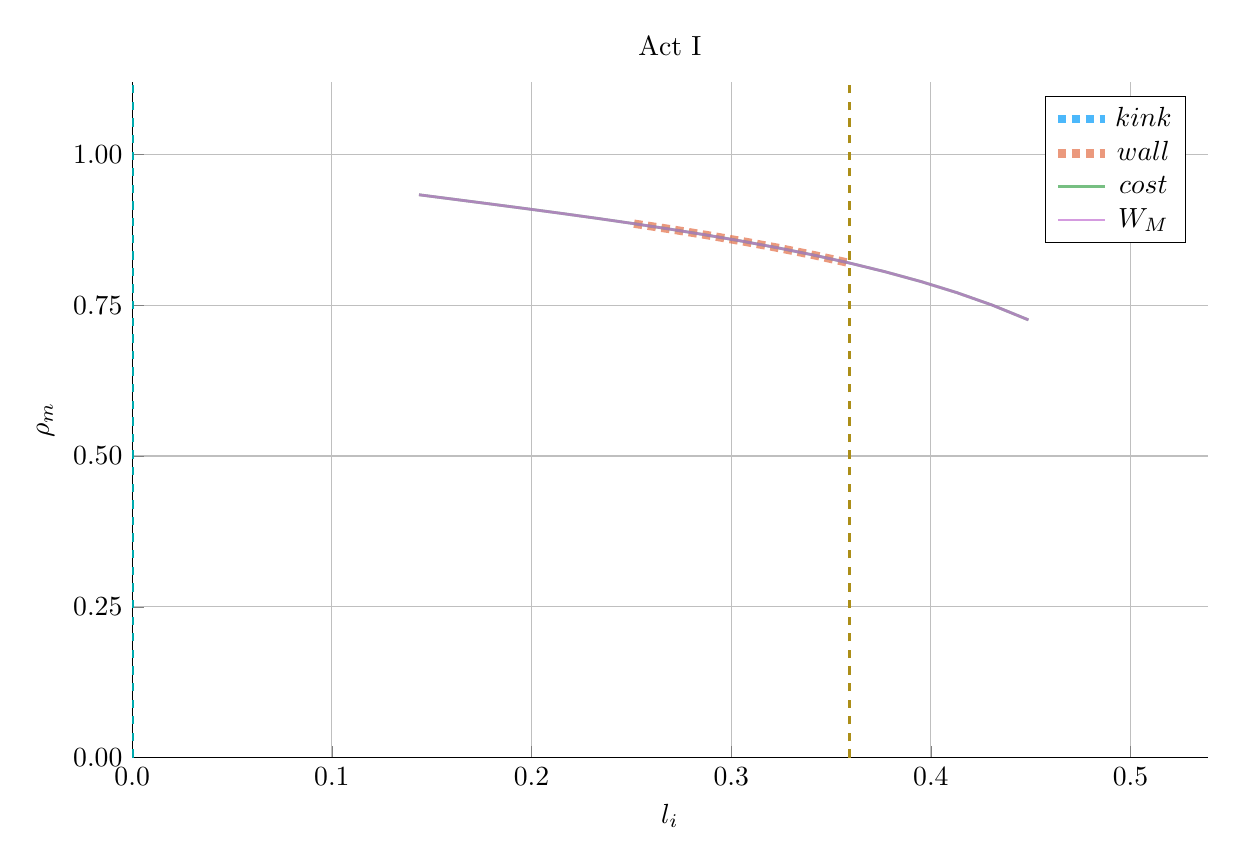
\begin{tikzpicture}[]
\begin{axis}[height = {101.6mm}, ylabel = {${\rho}_{m}$}, title = {Act I}, xmin = {0.0}, xmax = {0.5385899999999999}, ymax = {1.119646537068762}, xlabel = {${l}_{i}$}, {unbounded coords=jump, scaled x ticks = false, xticklabel style={rotate = 0}, xmajorgrids = true, xtick = {0.0,0.1,0.2,0.30000000000000004,0.4,0.5}, xticklabels = {0.0,0.1,0.2,0.3,0.4,0.5}, xtick align = inside, axis lines* = left, scaled y ticks = false, yticklabel style={rotate = 0}, ymajorgrids = true, ytick = {0.0,0.25,0.5,0.75,1.0}, yticklabels = {0.00,0.25,0.50,0.75,1.00}, ytick align = inside, axis lines* = left,     xshift = 0.0mm,
    yshift = 0.0mm,
    axis background/.style={fill={rgb,1:red,1.00000000;green,1.00000000;blue,1.00000000}}
, colorbar style={title=}}, ymin = {0.0}, width = {152.4mm}]\addplot+ [color = {rgb,1:red,0.00000000;green,0.60560316;blue,0.97868012},
draw opacity=0.7,
line width=3,
dotted,mark = none,
mark size = 2.0,
mark options = {
    color = {rgb,1:red,0.00000000;green,0.00000000;blue,0.00000000}, draw opacity = 0.7,
    fill = {rgb,1:red,0.00000000;green,0.60560316;blue,0.97868012}, fill opacity = 0.7,
    line width = 1,
    rotate = 0,
    solid
}]coordinates {
(0.251342, 0.8851086012444654)
};
\addlegendentry{$kink$}
\addplot+ [color = {rgb,1:red,0.88887350;green,0.43564919;blue,0.27812294},
draw opacity=0.7,
line width=3,
dotted,mark = none,
mark size = 2.0,
mark options = {
    color = {rgb,1:red,0.00000000;green,0.00000000;blue,0.00000000}, draw opacity = 0.7,
    fill = {rgb,1:red,0.88887350;green,0.43564919;blue,0.27812294}, fill opacity = 0.7,
    line width = 1,
    rotate = 0,
    solid
}]coordinates {
(0.251342, 0.8851086012444652)
(0.269295, 0.87606986359606)
(0.287248, 0.8664841109943121)
(0.305201, 0.8562356045511645)
(0.323154, 0.8451895999929044)
(0.341107, 0.8331857572197536)
(0.35906, 0.8200293573708509)
};
\addlegendentry{$wall$}
\addplot+ [color = {rgb,1:red,0.24222430;green,0.64327509;blue,0.30444865},
draw opacity=0.7,
line width=1,
solid,mark = none,
mark size = 2.0,
mark options = {
    color = {rgb,1:red,0.00000000;green,0.00000000;blue,0.00000000}, draw opacity = 0.7,
    fill = {rgb,1:red,0.24222430;green,0.64327509;blue,0.30444865}, fill opacity = 0.7,
    line width = 1,
    rotate = 0,
    solid
}]coordinates {
(0.143624, 0.9330387808906351)
(0.161577, 0.9253838422375279)
(0.17953, 0.917702462935453)
(0.197483, 0.9099154043022427)
(0.215436, 0.9019425781129675)
(0.233389, 0.8937021639390689)
(0.251342, 0.8851086012444653)
(0.269295, 0.8760698635960599)
(0.287248, 0.8664841109943121)
(0.305201, 0.8562356045511645)
(0.323154, 0.8451895999929047)
(0.341107, 0.8331857572197536)
(0.35906, 0.820029357370851)
(0.377013, 0.8054792350807263)
(0.394966, 0.7892306944297426)
(0.412919, 0.7708905627422878)
(0.430872, 0.7499395022888798)
(0.448825, 0.7256727825282991)
};
\addlegendentry{$cost$}
\addplot+ [color = {rgb,1:red,0.76444018;green,0.44411178;blue,0.82429754},
draw opacity=0.7,
line width=1,
solid,mark = none,
mark size = 2.0,
mark options = {
    color = {rgb,1:red,0.00000000;green,0.00000000;blue,0.00000000}, draw opacity = 0.7,
    fill = {rgb,1:red,0.76444018;green,0.44411178;blue,0.82429754}, fill opacity = 0.7,
    line width = 1,
    rotate = 0,
    solid
}]coordinates {
(0.143624, 0.933038780890635)
(0.161577, 0.925383842237528)
(0.17953, 0.9177024629354528)
(0.197483, 0.9099154043022427)
(0.215436, 0.9019425781129675)
(0.233389, 0.8937021639390689)
(0.251342, 0.8851086012444654)
(0.269295, 0.8760698635960601)
(0.287248, 0.8664841109943121)
(0.305201, 0.8562356045511644)
(0.323154, 0.8451895999929045)
(0.341107, 0.8331857572197536)
(0.35906, 0.8200293573708509)
(0.377013, 0.8054792350807263)
(0.394966, 0.7892306944297426)
(0.412919, 0.7708905627422878)
(0.430872, 0.74993950228888)
(0.448825, 0.7256727825282994)
};
\addlegendentry{$W_M$}
\addplot+ [color = {rgb,1:red,0.67554396;green,0.55566233;blue,0.09423434},
draw opacity=1.0,
line width=1,
dashed,mark = none,
mark size = 2.0,
mark options = {
    color = {rgb,1:red,0.00000000;green,0.00000000;blue,0.00000000}, draw opacity = 1.0,
    fill = {rgb,1:red,0.67554396;green,0.55566233;blue,0.09423434}, fill opacity = 1.0,
    line width = 1,
    rotate = 0,
    solid
},forget plot]coordinates {
(0.35906, 0.0)
(0.35906, 1.119646537068762)
};
\addplot+ [color = {rgb,1:red,0.00000048;green,0.66575898;blue,0.68099695},
draw opacity=1.0,
line width=1,
dashed,mark = none,
mark size = 2.0,
mark options = {
    color = {rgb,1:red,0.00000000;green,0.00000000;blue,0.00000000}, draw opacity = 1.0,
    fill = {rgb,1:red,0.00000048;green,0.66575898;blue,0.68099695}, fill opacity = 1.0,
    line width = 1,
    rotate = 0,
    solid
},forget plot]coordinates {
(0.0, 0.0)
(0.0, 1.119646537068762)
};
\addplot+ [color = {rgb,1:red,0.00000048;green,0.66575898;blue,0.68099695},
draw opacity=1.0,
line width=1,
dashed,mark = none,
mark size = 2.0,
mark options = {
    color = {rgb,1:red,0.00000000;green,0.00000000;blue,0.00000000}, draw opacity = 1.0,
    fill = {rgb,1:red,0.00000048;green,0.66575898;blue,0.68099695}, fill opacity = 1.0,
    line width = 1,
    rotate = 0,
    solid
},forget plot]coordinates {
(0.71812, 0.0)
(0.71812, 1.119646537068762)
};
\end{axis}

\end{tikzpicture}

		\end{adjustbox}
        \caption{Act I Peak Radius}
    \end{subfigure}
    \hfill
    \begin{subfigure}[t]{0.45\textwidth}
        \centering
		\begin{adjustbox}{width=\textwidth}
			\Large
			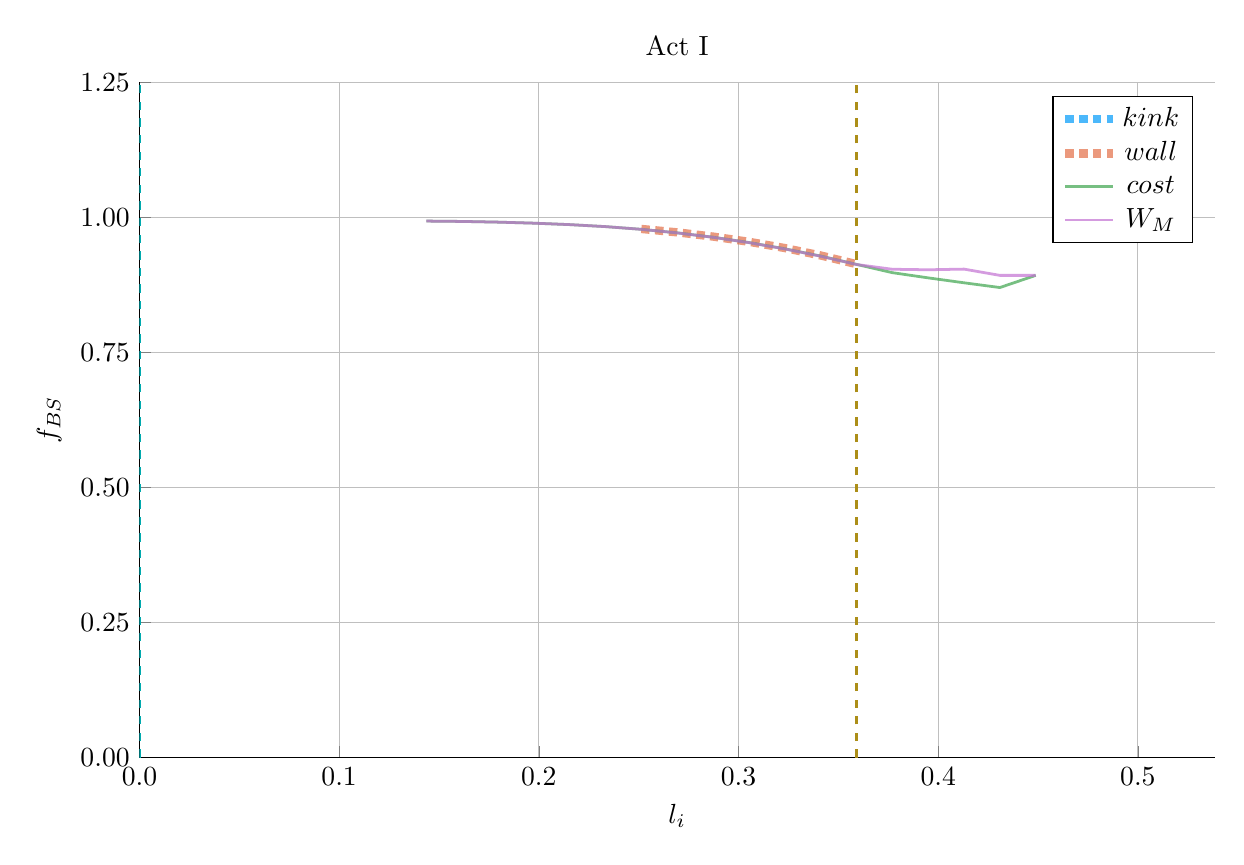
\begin{tikzpicture}[]
\begin{axis}[height = {101.6mm}, ylabel = {${f}_{BS}$}, title = {Act I}, xmin = {0.0}, xmax = {0.5385899999999999}, ymax = {1.25}, xlabel = {${l}_{i}$}, {unbounded coords=jump, scaled x ticks = false, xticklabel style={rotate = 0}, xmajorgrids = true, xtick = {0.0,0.1,0.2,0.30000000000000004,0.4,0.5}, xticklabels = {0.0,0.1,0.2,0.3,0.4,0.5}, xtick align = inside, axis lines* = left, scaled y ticks = false, yticklabel style={rotate = 0}, ymajorgrids = true, ytick = {0.0,0.25,0.5,0.75,1.0,1.25}, yticklabels = {0.00,0.25,0.50,0.75,1.00,1.25}, ytick align = inside, axis lines* = left,     xshift = 0.0mm,
    yshift = 0.0mm,
    axis background/.style={fill={rgb,1:red,1.00000000;green,1.00000000;blue,1.00000000}}
, colorbar style={title=}}, ymin = {0.0}, width = {152.4mm}]\addplot+ [color = {rgb,1:red,0.00000000;green,0.60560316;blue,0.97868012},
draw opacity=0.7,
line width=3,
dotted,mark = none,
mark size = 2.0,
mark options = {
    color = {rgb,1:red,0.00000000;green,0.00000000;blue,0.00000000}, draw opacity = 0.7,
    fill = {rgb,1:red,0.00000000;green,0.60560316;blue,0.97868012}, fill opacity = 0.7,
    line width = 1,
    rotate = 0,
    solid
}]coordinates {
(0.251342, 0.9696030028328079)
};
\addlegendentry{$kink$}
\addplot+ [color = {rgb,1:red,0.88887350;green,0.43564919;blue,0.27812294},
draw opacity=0.7,
line width=3,
dotted,mark = none,
mark size = 2.0,
mark options = {
    color = {rgb,1:red,0.00000000;green,0.00000000;blue,0.00000000}, draw opacity = 0.7,
    fill = {rgb,1:red,0.88887350;green,0.43564919;blue,0.27812294}, fill opacity = 0.7,
    line width = 1,
    rotate = 0,
    solid
}]coordinates {
(0.251342, 0.978390751679801)
(0.269295, 0.9720986271034725)
(0.287248, 0.9642571574237495)
(0.305201, 0.9546457701988796)
(0.323154, 0.9430671446437034)
(0.341107, 0.9293485896194813)
(0.35906, 0.9133153826691774)
};
\addlegendentry{$wall$}
\addplot+ [color = {rgb,1:red,0.24222430;green,0.64327509;blue,0.30444865},
draw opacity=0.7,
line width=1,
solid,mark = none,
mark size = 2.0,
mark options = {
    color = {rgb,1:red,0.00000000;green,0.00000000;blue,0.00000000}, draw opacity = 0.7,
    fill = {rgb,1:red,0.24222430;green,0.64327509;blue,0.30444865}, fill opacity = 0.7,
    line width = 1,
    rotate = 0,
    solid
}]coordinates {
(0.143624, 0.9929804464046398)
(0.161577, 0.9923030142510472)
(0.17953, 0.991015050866744)
(0.197483, 0.9890965947845473)
(0.215436, 0.9864075747184604)
(0.233389, 0.9827200373518228)
(0.251342, 0.9777143624359533)
(0.269295, 0.9711704934003316)
(0.287248, 0.9630778239630123)
(0.305201, 0.9532824413525581)
(0.323154, 0.9416818430664083)
(0.341107, 0.9282170879023031)
(0.35906, 0.9128235165006966)
(0.377013, 0.897511189122376)
(0.394966, 0.8878778890807072)
(0.412919, 0.8787493121917717)
(0.430872, 0.8699777046780948)
(0.448825, 0.8924895907906419)
};
\addlegendentry{$cost$}
\addplot+ [color = {rgb,1:red,0.76444018;green,0.44411178;blue,0.82429754},
draw opacity=0.7,
line width=1,
solid,mark = none,
mark size = 2.0,
mark options = {
    color = {rgb,1:red,0.00000000;green,0.00000000;blue,0.00000000}, draw opacity = 0.7,
    fill = {rgb,1:red,0.76444018;green,0.44411178;blue,0.82429754}, fill opacity = 0.7,
    line width = 1,
    rotate = 0,
    solid
}]coordinates {
(0.143624, 0.9929810667704344)
(0.161577, 0.9923050590584696)
(0.17953, 0.99101779250524)
(0.197483, 0.9890988108125024)
(0.215436, 0.9864065443793834)
(0.233389, 0.9827091710899777)
(0.251342, 0.9776791928925961)
(0.269295, 0.9710989320429835)
(0.287248, 0.9629528965707805)
(0.305201, 0.9530910256378358)
(0.323154, 0.9414257974679184)
(0.341107, 0.9279315661369091)
(0.35906, 0.912636558725213)
(0.377013, 0.903811645293124)
(0.394966, 0.9028566905661166)
(0.412919, 0.9040751250575536)
(0.430872, 0.892489590790642)
(0.448825, 0.8924895907906422)
};
\addlegendentry{$W_M$}
\addplot+ [color = {rgb,1:red,0.67554396;green,0.55566233;blue,0.09423434},
draw opacity=1.0,
line width=1,
dashed,mark = none,
mark size = 2.0,
mark options = {
    color = {rgb,1:red,0.00000000;green,0.00000000;blue,0.00000000}, draw opacity = 1.0,
    fill = {rgb,1:red,0.67554396;green,0.55566233;blue,0.09423434}, fill opacity = 1.0,
    line width = 1,
    rotate = 0,
    solid
},forget plot]coordinates {
(0.35906, 0.0)
(0.35906, 1.25)
};
\addplot+ [color = {rgb,1:red,0.00000048;green,0.66575898;blue,0.68099695},
draw opacity=1.0,
line width=1,
dashed,mark = none,
mark size = 2.0,
mark options = {
    color = {rgb,1:red,0.00000000;green,0.00000000;blue,0.00000000}, draw opacity = 1.0,
    fill = {rgb,1:red,0.00000048;green,0.66575898;blue,0.68099695}, fill opacity = 1.0,
    line width = 1,
    rotate = 0,
    solid
},forget plot]coordinates {
(0.0, 0.0)
(0.0, 1.25)
};
\addplot+ [color = {rgb,1:red,0.00000048;green,0.66575898;blue,0.68099695},
draw opacity=1.0,
line width=1,
dashed,mark = none,
mark size = 2.0,
mark options = {
    color = {rgb,1:red,0.00000000;green,0.00000000;blue,0.00000000}, draw opacity = 1.0,
    fill = {rgb,1:red,0.00000048;green,0.66575898;blue,0.68099695}, fill opacity = 1.0,
    line width = 1,
    rotate = 0,
    solid
},forget plot]coordinates {
(0.71812, 0.0)
(0.71812, 1.25)
};
\end{axis}

\end{tikzpicture}

		\end{adjustbox}
        \caption{Act I Bootstrap Fraction}
    \end{subfigure}
    \hfill \hfill ~\\ ~\\ ~\\ ~\\
    \hfill 
    \begin{subfigure}[t]{0.45\textwidth}
        \centering
		\begin{adjustbox}{width=\textwidth}
			\Large
			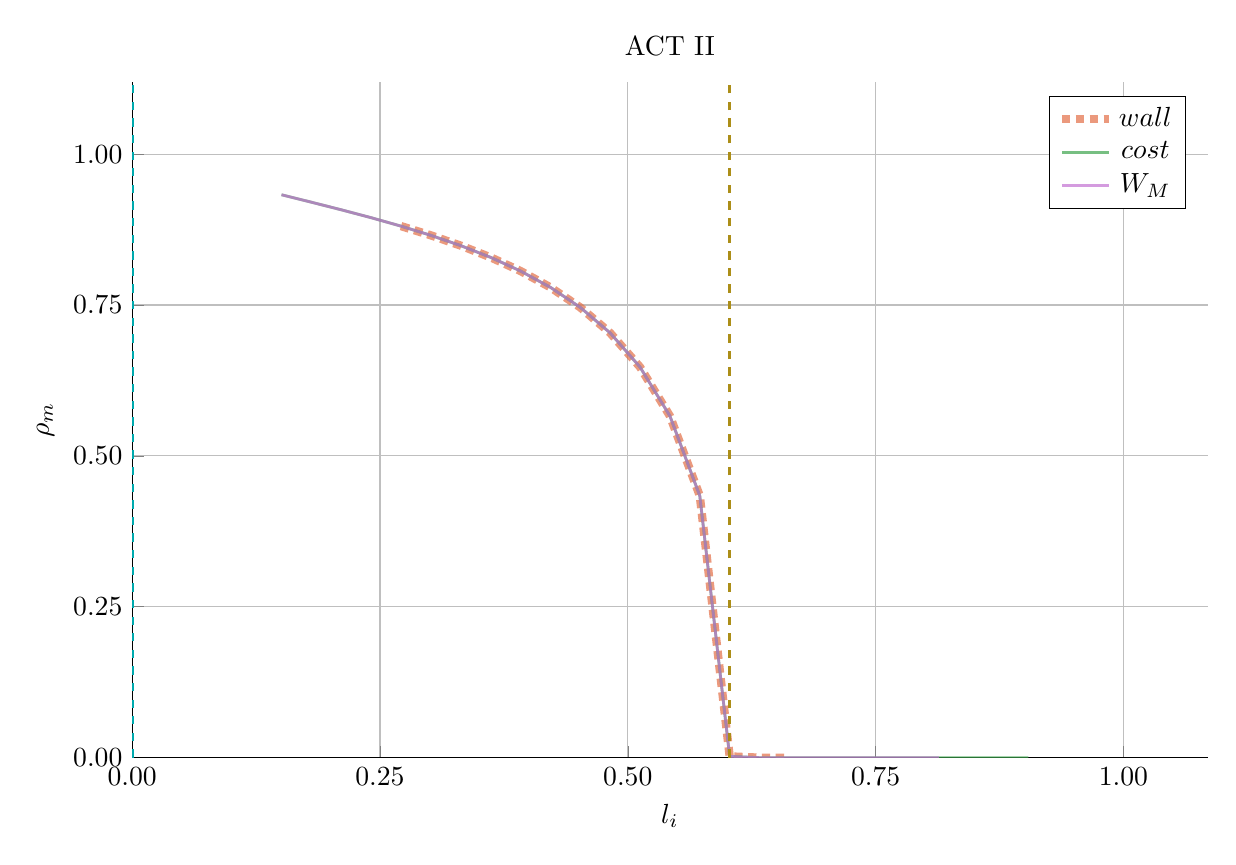
\begin{tikzpicture}[]
\begin{axis}[height = {101.6mm}, ylabel = {${\rho}_{m}$}, title = {ACT II}, xmin = {0.0}, xmax = {1.0849499999999999}, ymax = {1.1191149984068893}, xlabel = {${l}_{i}$}, {unbounded coords=jump, scaled x ticks = false, xticklabel style={rotate = 0}, xmajorgrids = true, xtick = {0.0,0.25,0.5,0.75,1.0}, xticklabels = {0.00,0.25,0.50,0.75,1.00}, xtick align = inside, axis lines* = left, scaled y ticks = false, yticklabel style={rotate = 0}, ymajorgrids = true, ytick = {0.0,0.25,0.5,0.75,1.0}, yticklabels = {0.00,0.25,0.50,0.75,1.00}, ytick align = inside, axis lines* = left,     xshift = 0.0mm,
    yshift = 0.0mm,
    axis background/.style={fill={rgb,1:red,1.00000000;green,1.00000000;blue,1.00000000}}
, colorbar style={title=}}, ymin = {0.0}, width = {152.4mm}]\addplot+ [color = {rgb,1:red,0.88887350;green,0.43564919;blue,0.27812294},
draw opacity=0.7,
line width=3,
dotted,mark = none,
mark size = 2.0,
mark options = {
    color = {rgb,1:red,0.00000000;green,0.00000000;blue,0.00000000}, draw opacity = 0.7,
    fill = {rgb,1:red,0.88887350;green,0.43564919;blue,0.27812294}, fill opacity = 0.7,
    line width = 1,
    rotate = 0,
    solid
}]coordinates {
(0.2712375, 0.8806148204118965)
(0.301375, 0.8653360652102908)
(0.3315125, 0.8482916552470681)
(0.36165, 0.8288701250926883)
(0.3917875, 0.8062408264324945)
(0.421925, 0.7792148539986927)
(0.4520625, 0.7459941408070427)
(0.4822, 0.7036750754408452)
(0.5123375, 0.6471402309036279)
(0.542475, 0.5660883461899422)
(0.5726125, 0.43389574174946466)
(0.60275, 0.002161634542349489)
(0.6328875, 0.0)
(0.663025, 0.0)
};
\addlegendentry{$wall$}
\addplot+ [color = {rgb,1:red,0.24222430;green,0.64327509;blue,0.30444865},
draw opacity=0.7,
line width=1,
solid,mark = none,
mark size = 2.0,
mark options = {
    color = {rgb,1:red,0.00000000;green,0.00000000;blue,0.00000000}, draw opacity = 0.7,
    fill = {rgb,1:red,0.24222430;green,0.64327509;blue,0.30444865}, fill opacity = 0.7,
    line width = 1,
    rotate = 0,
    solid
}]coordinates {
(0.1506875, 0.9325958320057411)
(0.180825, 0.9202502226250152)
(0.2109625, 0.9076981644853267)
(0.2411, 0.8946038489442804)
(0.2712375, 0.8806148204118966)
(0.301375, 0.8653360652102907)
(0.3315125, 0.848291655247068)
(0.36165, 0.8288701250926882)
(0.3917875, 0.8062408264324945)
(0.421925, 0.7792148539986927)
(0.4520625, 0.7459941408070427)
(0.4822, 0.7036750754408454)
(0.5123375, 0.6471402309036269)
(0.542475, 0.5660883461899405)
(0.5726125, 0.43389574174946843)
(0.60275, 0.00216163454214405)
(0.6328875, 0.0)
(0.663025, 0.0)
(0.7233, 0.0)
(0.7534375, 0.0)
(0.783575, 0.0)
(0.8137125, 0.0)
(0.84385, 0.0)
(0.8739875, 0.0)
(0.904125, 0.0)
};
\addlegendentry{$cost$}
\addplot+ [color = {rgb,1:red,0.76444018;green,0.44411178;blue,0.82429754},
draw opacity=0.7,
line width=1,
solid,mark = none,
mark size = 2.0,
mark options = {
    color = {rgb,1:red,0.00000000;green,0.00000000;blue,0.00000000}, draw opacity = 0.7,
    fill = {rgb,1:red,0.76444018;green,0.44411178;blue,0.82429754}, fill opacity = 0.7,
    line width = 1,
    rotate = 0,
    solid
}]coordinates {
(0.1506875, 0.9325958320057409)
(0.180825, 0.9202502226250147)
(0.2109625, 0.9076981644853267)
(0.2411, 0.8946038489442804)
(0.2712375, 0.8806148204118963)
(0.301375, 0.8653360652102908)
(0.3315125, 0.8482916552470682)
(0.36165, 0.8288701250926886)
(0.3917875, 0.8062408264324947)
(0.421925, 0.779214853998693)
(0.4520625, 0.7459941408070427)
(0.4822, 0.7036750754408455)
(0.5123375, 0.6471402309036273)
(0.542475, 0.5660883461899405)
(0.5726125, 0.43389574174946755)
(0.60275, 0.0021616345408086934)
(0.6328875, 0.0)
(0.663025, 0.0)
(0.7233, 0.0)
(0.7534375, 0.0)
(0.783575, 0.0)
(0.8137125, 0.0)
};
\addlegendentry{$W_M$}
\addplot+ [color = {rgb,1:red,0.67554396;green,0.55566233;blue,0.09423434},
draw opacity=1.0,
line width=1,
dashed,mark = none,
mark size = 2.0,
mark options = {
    color = {rgb,1:red,0.00000000;green,0.00000000;blue,0.00000000}, draw opacity = 1.0,
    fill = {rgb,1:red,0.67554396;green,0.55566233;blue,0.09423434}, fill opacity = 1.0,
    line width = 1,
    rotate = 0,
    solid
},forget plot]coordinates {
(0.60275, 0.0)
(0.60275, 1.1191149984068893)
};
\addplot+ [color = {rgb,1:red,0.00000048;green,0.66575898;blue,0.68099695},
draw opacity=1.0,
line width=1,
dashed,mark = none,
mark size = 2.0,
mark options = {
    color = {rgb,1:red,0.00000000;green,0.00000000;blue,0.00000000}, draw opacity = 1.0,
    fill = {rgb,1:red,0.00000048;green,0.66575898;blue,0.68099695}, fill opacity = 1.0,
    line width = 1,
    rotate = 0,
    solid
},forget plot]coordinates {
(0.0, 0.0)
(0.0, 1.1191149984068893)
};
\addplot+ [color = {rgb,1:red,0.00000048;green,0.66575898;blue,0.68099695},
draw opacity=1.0,
line width=1,
dashed,mark = none,
mark size = 2.0,
mark options = {
    color = {rgb,1:red,0.00000000;green,0.00000000;blue,0.00000000}, draw opacity = 1.0,
    fill = {rgb,1:red,0.00000048;green,0.66575898;blue,0.68099695}, fill opacity = 1.0,
    line width = 1,
    rotate = 0,
    solid
},forget plot]coordinates {
(1.2055, 0.0)
(1.2055, 1.1191149984068893)
};
\end{axis}

\end{tikzpicture}

		\end{adjustbox}
        \caption{Act II Peak Radius}
    \end{subfigure}
    \hfill
    \begin{subfigure}[t]{0.45\textwidth}
        \centering
		\begin{adjustbox}{width=\textwidth}
			\Large
			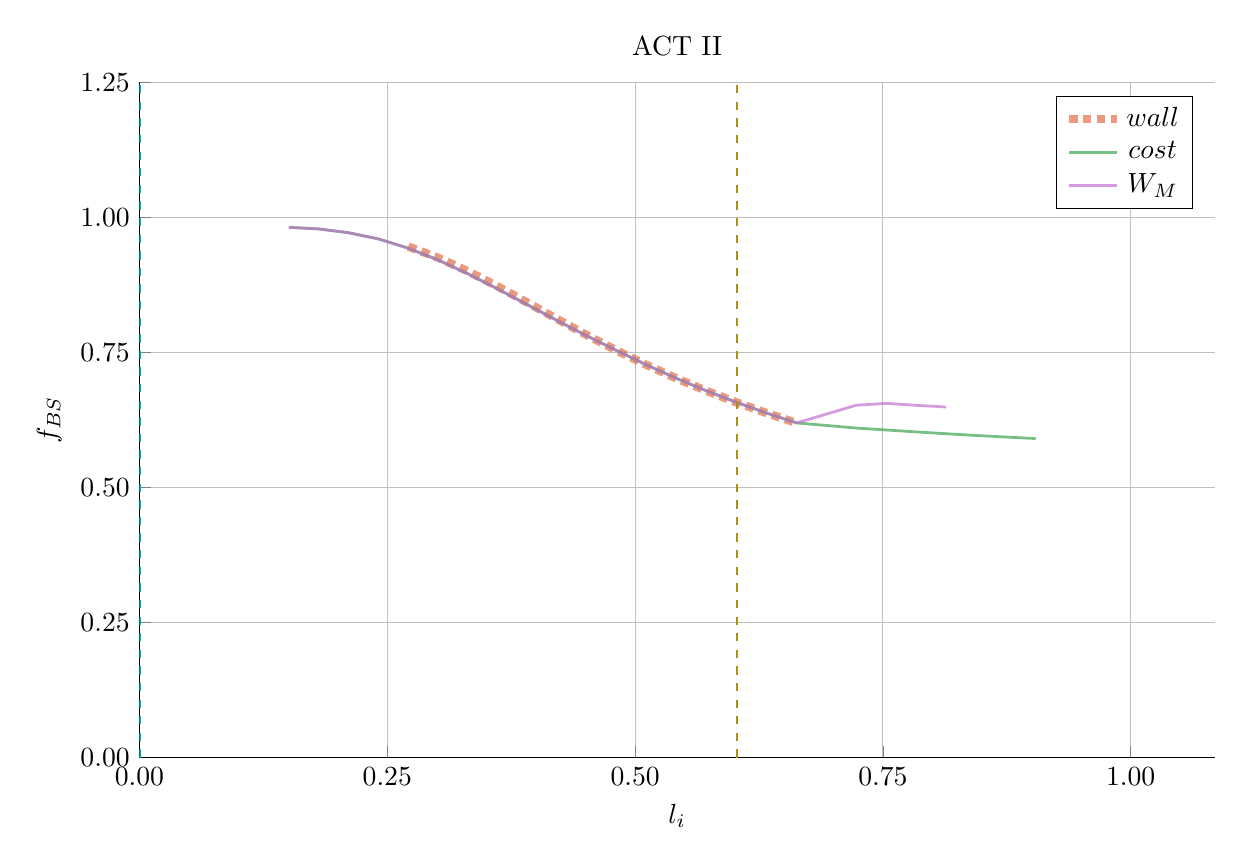
\begin{tikzpicture}[]
\begin{axis}[height = {101.6mm}, ylabel = {${f}_{BS}$}, title = {ACT II}, xmin = {0.0}, xmax = {1.0849499999999999}, ymax = {1.25}, xlabel = {${l}_{i}$}, {unbounded coords=jump, scaled x ticks = false, xticklabel style={rotate = 0}, xmajorgrids = true, xtick = {0.0,0.25,0.5,0.75,1.0}, xticklabels = {0.00,0.25,0.50,0.75,1.00}, xtick align = inside, axis lines* = left, scaled y ticks = false, yticklabel style={rotate = 0}, ymajorgrids = true, ytick = {0.0,0.25,0.5,0.75,1.0,1.25}, yticklabels = {0.00,0.25,0.50,0.75,1.00,1.25}, ytick align = inside, axis lines* = left,     xshift = 0.0mm,
    yshift = 0.0mm,
    axis background/.style={fill={rgb,1:red,1.00000000;green,1.00000000;blue,1.00000000}}
, colorbar style={title=}}, ymin = {0.0}, width = {152.4mm}]\addplot+ [color = {rgb,1:red,0.88887350;green,0.43564919;blue,0.27812294},
draw opacity=0.7,
line width=3,
dotted,mark = none,
mark size = 2.0,
mark options = {
    color = {rgb,1:red,0.00000000;green,0.00000000;blue,0.00000000}, draw opacity = 0.7,
    fill = {rgb,1:red,0.88887350;green,0.43564919;blue,0.27812294}, fill opacity = 0.7,
    line width = 1,
    rotate = 0,
    solid
}]coordinates {
(0.2712375, 0.945768815749713)
(0.301375, 0.9250106384697369)
(0.3315125, 0.8999898310074997)
(0.36165, 0.8717362821014283)
(0.3917875, 0.8416501471992826)
(0.421925, 0.811099919466637)
(0.4520625, 0.7811575032095794)
(0.4822, 0.7525898335408499)
(0.5123375, 0.7259971657203301)
(0.542475, 0.7012410038364986)
(0.5726125, 0.6783088266487727)
(0.60275, 0.6571060030654019)
(0.6328875, 0.6375068757553635)
(0.663025, 0.6193632746844691)
};
\addlegendentry{$wall$}
\addplot+ [color = {rgb,1:red,0.24222430;green,0.64327509;blue,0.30444865},
draw opacity=0.7,
line width=1,
solid,mark = none,
mark size = 2.0,
mark options = {
    color = {rgb,1:red,0.00000000;green,0.00000000;blue,0.00000000}, draw opacity = 0.7,
    fill = {rgb,1:red,0.24222430;green,0.64327509;blue,0.30444865}, fill opacity = 0.7,
    line width = 1,
    rotate = 0,
    solid
}]coordinates {
(0.1506875, 0.981343377436681)
(0.180825, 0.978396601376748)
(0.2109625, 0.9714184274346895)
(0.2411, 0.9599381301711771)
(0.2712375, 0.9427525343273128)
(0.301375, 0.9210032370912685)
(0.3315125, 0.8954095126207788)
(0.36165, 0.8672317152489013)
(0.3917875, 0.837863200045813)
(0.421925, 0.8084884612310679)
(0.4520625, 0.7799401100642639)
(0.4822, 0.7526478350077306)
(0.5123375, 0.7260661853694742)
(0.542475, 0.7013162910532953)
(0.5726125, 0.678387389033931)
(0.60275, 0.6571862028703379)
(0.6328875, 0.637588501426561)
(0.663025, 0.6194476020408427)
(0.7233, 0.6099474641801359)
(0.7534375, 0.6063857323409275)
(0.783575, 0.6028283872308784)
(0.8137125, 0.5994402215386627)
(0.84385, 0.5962607663212237)
(0.8739875, 0.593292640311373)
(0.904125, 0.5905270970377445)
};
\addlegendentry{$cost$}
\addplot+ [color = {rgb,1:red,0.76444018;green,0.44411178;blue,0.82429754},
draw opacity=0.7,
line width=1,
solid,mark = none,
mark size = 2.0,
mark options = {
    color = {rgb,1:red,0.00000000;green,0.00000000;blue,0.00000000}, draw opacity = 0.7,
    fill = {rgb,1:red,0.76444018;green,0.44411178;blue,0.82429754}, fill opacity = 0.7,
    line width = 1,
    rotate = 0,
    solid
}]coordinates {
(0.1506875, 0.9813536850683049)
(0.180825, 0.9784148538314168)
(0.2109625, 0.971433828275815)
(0.2411, 0.9599201850896092)
(0.2712375, 0.9426621091385493)
(0.301375, 0.9208121727384578)
(0.3315125, 0.8951317092257599)
(0.36165, 0.8669198983037378)
(0.3917875, 0.8375793628181188)
(0.421925, 0.8082860600578722)
(0.4520625, 0.7798449919220848)
(0.4822, 0.7526503453313852)
(0.5123375, 0.7260740832005117)
(0.542475, 0.7013272369810847)
(0.5726125, 0.678398847271037)
(0.60275, 0.657196611307558)
(0.6328875, 0.6375969323800256)
(0.663025, 0.6194546402361586)
(0.7233, 0.6522504808869147)
(0.7534375, 0.6556416125520123)
(0.783575, 0.6519819046272082)
(0.8137125, 0.6489284946814213)
};
\addlegendentry{$W_M$}
\addplot+ [color = {rgb,1:red,0.67554396;green,0.55566233;blue,0.09423434},
draw opacity=1.0,
line width=1,
dashed,mark = none,
mark size = 2.0,
mark options = {
    color = {rgb,1:red,0.00000000;green,0.00000000;blue,0.00000000}, draw opacity = 1.0,
    fill = {rgb,1:red,0.67554396;green,0.55566233;blue,0.09423434}, fill opacity = 1.0,
    line width = 1,
    rotate = 0,
    solid
},forget plot]coordinates {
(0.60275, 0.0)
(0.60275, 1.25)
};
\addplot+ [color = {rgb,1:red,0.00000048;green,0.66575898;blue,0.68099695},
draw opacity=1.0,
line width=1,
dashed,mark = none,
mark size = 2.0,
mark options = {
    color = {rgb,1:red,0.00000000;green,0.00000000;blue,0.00000000}, draw opacity = 1.0,
    fill = {rgb,1:red,0.00000048;green,0.66575898;blue,0.68099695}, fill opacity = 1.0,
    line width = 1,
    rotate = 0,
    solid
},forget plot]coordinates {
(0.0, 0.0)
(0.0, 1.25)
};
\addplot+ [color = {rgb,1:red,0.00000048;green,0.66575898;blue,0.68099695},
draw opacity=1.0,
line width=1,
dashed,mark = none,
mark size = 2.0,
mark options = {
    color = {rgb,1:red,0.00000000;green,0.00000000;blue,0.00000000}, draw opacity = 1.0,
    fill = {rgb,1:red,0.00000048;green,0.66575898;blue,0.68099695}, fill opacity = 1.0,
    line width = 1,
    rotate = 0,
    solid
},forget plot]coordinates {
(1.2055, 0.0)
(1.2055, 1.25)
};
\end{axis}

\end{tikzpicture}

		\end{adjustbox}
        \caption{Act II Bootstrap Fraction}
    \end{subfigure}
    \hfill \hfill ~\\ ~\\ ~\\ ~\\
    \caption{Internal Inductance Sensitivities}
    \label{fig:inductance_sensitivities}
\end{figure*}

\subsubsection{Contextualizing the H-Factor}

From before, increasing the H-factor always led to more cost effective steady-state reactors. This is because the enhanced confinement allows for smaller machines. This was already heavily explored in \cref{fig:act_h_cost}. These plots also show that steady state reactors would not be physically possible using a default H factor of one! In other words, steady-state tokamaks require some technical advancement before they can ever be used as fusion reactors. The same cannot be said for pulsed machines.

For pulsed reactors, increasing H always reduces capital cost, but may actually increase the cost-per-watt. The reason for this is because fusion powers are much smaller in pulsed machines. This interesting result demonstrates the unusual behaviors of highly non-linear systems: masterclass intuition may not match model results.

\begin{figure*}
    \centering
    \hfill 
    \begin{subfigure}[t]{0.45\textwidth}
        \centering
		\begin{adjustbox}{width=\textwidth}
			\Large
			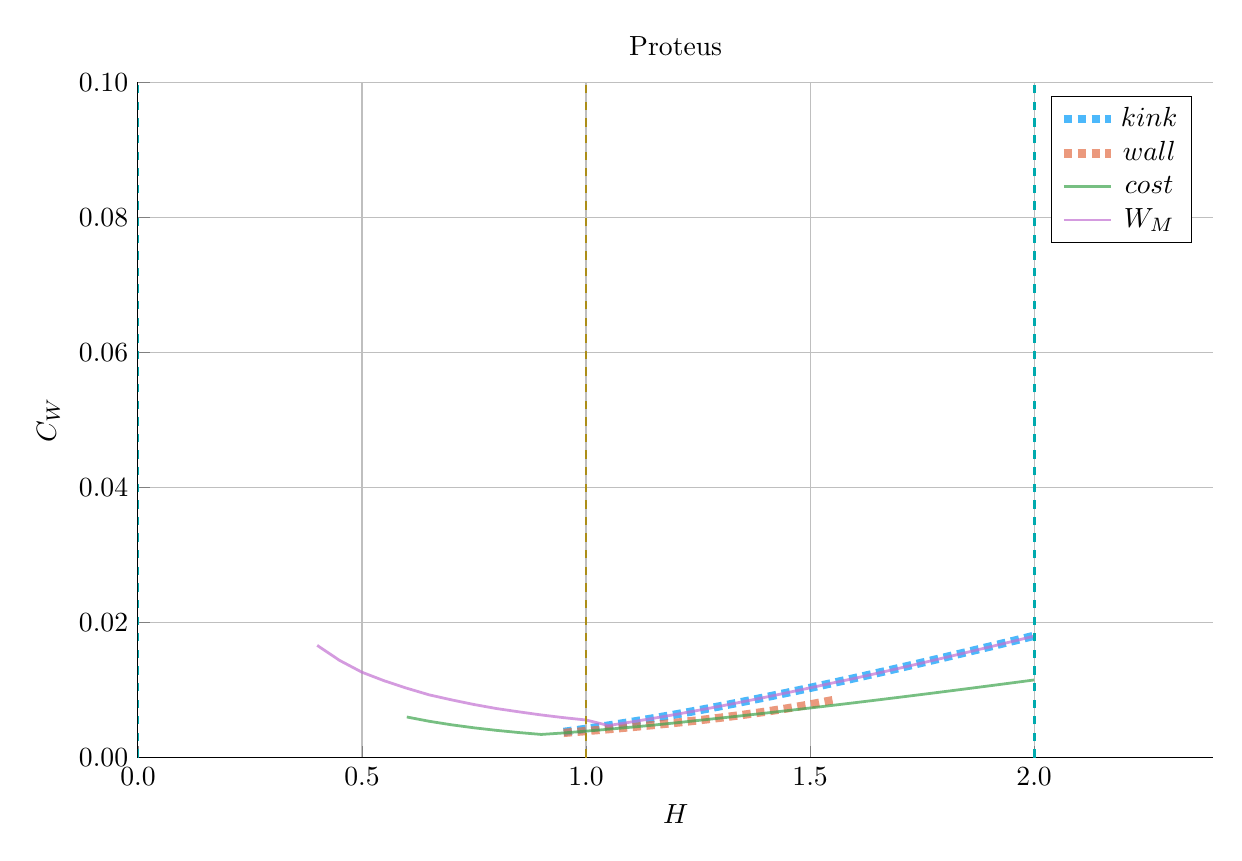
\begin{tikzpicture}[]
\begin{axis}[height = {101.6mm}, ylabel = {${C}_{W}$}, title = {Proteus}, xmin = {0.0}, xmax = {2.4}, ymax = {0.1}, xlabel = {${H}$}, {unbounded coords=jump, scaled x ticks = false, xticklabel style={rotate = 0}, xmajorgrids = true, xtick = {0.0,0.5,1.0,1.5,2.0}, xticklabels = {0.0,0.5,1.0,1.5,2.0}, xtick align = inside, axis lines* = left, scaled y ticks = false, yticklabel style={rotate = 0}, ymajorgrids = true, ytick = {0.0,0.02,0.04,0.06,0.08,0.1}, yticklabels = {0.00,0.02,0.04,0.06,0.08,0.10}, ytick align = inside, axis lines* = left,     xshift = 0.0mm,
    yshift = 0.0mm,
    axis background/.style={fill={rgb,1:red,1.00000000;green,1.00000000;blue,1.00000000}}
, colorbar style={title=}}, ymin = {0.0}, width = {152.4mm}]\addplot+ [color = {rgb,1:red,0.00000000;green,0.60560316;blue,0.97868012},
draw opacity=0.7,
line width=3,
dotted,mark = none,
mark size = 2.0,
mark options = {
    color = {rgb,1:red,0.00000000;green,0.00000000;blue,0.00000000}, draw opacity = 0.7,
    fill = {rgb,1:red,0.00000000;green,0.60560316;blue,0.97868012}, fill opacity = 0.7,
    line width = 1,
    rotate = 0,
    solid
}]coordinates {
(0.95, 0.003813408855944681)
(1.0, 0.004265648977267023)
(1.05, 0.004752668146662768)
(1.1, 0.005271613491882024)
(1.15, 0.0058201404107927224)
(1.2, 0.006396183772570443)
(1.25, 0.006997835782236724)
(1.3, 0.0076232953530691394)
(1.35, 0.008270841443829582)
(1.4, 0.008938822056036154)
(1.45, 0.009625650669899507)
(1.5, 0.010329806212420205)
(1.55, 0.011049834442804687)
(1.6, 0.01178434962200705)
(1.65, 0.012532035875733484)
(1.7, 0.013291647978620374)
(1.75, 0.014062011464491491)
(1.8, 0.014842022069343515)
(1.85, 0.015630644567704882)
(1.9, 0.016426911088780652)
(1.95, 0.01722991900758117)
(2.0, 0.018038828505044485)
};
\addlegendentry{$kink$}
\addplot+ [color = {rgb,1:red,0.88887350;green,0.43564919;blue,0.27812294},
draw opacity=0.7,
line width=3,
dotted,mark = none,
mark size = 2.0,
mark options = {
    color = {rgb,1:red,0.00000000;green,0.00000000;blue,0.00000000}, draw opacity = 0.7,
    fill = {rgb,1:red,0.88887350;green,0.43564919;blue,0.27812294}, fill opacity = 0.7,
    line width = 1,
    rotate = 0,
    solid
}]coordinates {
(0.95, 0.003666946839795346)
(1.0, 0.0039361219986185116)
(1.05, 0.004218135275999639)
(1.1, 0.004515096432908966)
(1.15, 0.004829564370185442)
(1.2, 0.005164630631420896)
(1.25, 0.005524018627298141)
(1.3, 0.005912200100926477)
(1.35, 0.006334527895446957)
(1.4, 0.0067973755206943215)
(1.45, 0.007308245119986767)
(1.5, 0.00787570051155573)
(1.55, 0.008508529553855641)
};
\addlegendentry{$wall$}
\addplot+ [color = {rgb,1:red,0.24222430;green,0.64327509;blue,0.30444865},
draw opacity=0.7,
line width=1,
solid,mark = none,
mark size = 2.0,
mark options = {
    color = {rgb,1:red,0.00000000;green,0.00000000;blue,0.00000000}, draw opacity = 0.7,
    fill = {rgb,1:red,0.24222430;green,0.64327509;blue,0.30444865}, fill opacity = 0.7,
    line width = 1,
    rotate = 0,
    solid
}]coordinates {
(0.6, 0.006019077014978464)
(0.65, 0.005385886897052109)
(0.7, 0.004860407749972578)
(0.75, 0.004418196734456711)
(0.8, 0.004041544969852703)
(0.85, 0.003717336065565805)
(0.9, 0.0034356659911458534)
(0.95, 0.00365825706976454)
(1.0, 0.0039266466317365994)
(1.05, 0.004207796818733193)
(1.1, 0.004503801283721318)
(1.15, 0.004817199216122392)
(1.2, 0.005151057850506862)
(1.25, 0.005509070949676484)
(1.3, 0.005863026988877018)
(1.35, 0.006224389157755859)
(1.4, 0.006593207598014843)
(1.45, 0.006969199536400499)
(1.5, 0.007352115069518713)
(1.55, 0.007741609312154366)
(1.6, 0.00813752027135465)
(1.65, 0.008539562167230447)
(1.7, 0.008947416585436338)
(1.75, 0.009360876610350743)
(1.8, 0.009779664536750452)
(1.85, 0.010203472803315714)
(1.9, 0.010632108441138773)
(1.95, 0.011065202739676538)
(2.0, 0.011502557051621561)
};
\addlegendentry{$cost$}
\addplot+ [color = {rgb,1:red,0.76444018;green,0.44411178;blue,0.82429754},
draw opacity=0.7,
line width=1,
solid,mark = none,
mark size = 2.0,
mark options = {
    color = {rgb,1:red,0.00000000;green,0.00000000;blue,0.00000000}, draw opacity = 0.7,
    fill = {rgb,1:red,0.76444018;green,0.44411178;blue,0.82429754}, fill opacity = 0.7,
    line width = 1,
    rotate = 0,
    solid
}]coordinates {
(0.4, 0.016624506347810413)
(0.45, 0.01439742578556475)
(0.5, 0.012644217189325842)
(0.55, 0.011371080089774575)
(0.6, 0.010278715067173667)
(0.65, 0.009296214397712091)
(0.7, 0.008552733752259851)
(0.75, 0.0078672896176646)
(0.8, 0.007271126613604533)
(0.85, 0.0067844273503643825)
(0.9, 0.00632204592081946)
(0.95, 0.0059213060667176)
(1.0, 0.005573526121297312)
(1.05, 0.0047558341929866445)
(1.1, 0.005275181950267517)
(1.15, 0.005824086044617991)
(1.2, 0.006400480635204526)
(1.25, 0.007002459241165188)
(1.3, 0.007628220586818361)
(1.35, 0.008276043128948368)
(1.4, 0.008944274286954117)
(1.45, 0.009631327032234294)
(1.5, 0.01033567995641998)
(1.55, 0.011055878583326427)
(1.6, 0.011750726400721365)
(1.65, 0.012496629078464067)
(1.7, 0.013254462253826522)
(1.75, 0.014023053840465982)
(1.8, 0.014801301333054103)
(1.85, 0.015588171303544868)
(1.9, 0.016382696875007947)
(1.95, 0.017183976997357922)
(2.0, 0.01799117249644402)
};
\addlegendentry{$W_M$}
\addplot+ [color = {rgb,1:red,0.67554396;green,0.55566233;blue,0.09423434},
draw opacity=1.0,
line width=1,
dashed,mark = none,
mark size = 2.0,
mark options = {
    color = {rgb,1:red,0.00000000;green,0.00000000;blue,0.00000000}, draw opacity = 1.0,
    fill = {rgb,1:red,0.67554396;green,0.55566233;blue,0.09423434}, fill opacity = 1.0,
    line width = 1,
    rotate = 0,
    solid
},forget plot]coordinates {
(1.0, 0.0)
(1.0, 0.1)
};
\addplot+ [color = {rgb,1:red,0.00000048;green,0.66575898;blue,0.68099695},
draw opacity=1.0,
line width=1,
dashed,mark = none,
mark size = 2.0,
mark options = {
    color = {rgb,1:red,0.00000000;green,0.00000000;blue,0.00000000}, draw opacity = 1.0,
    fill = {rgb,1:red,0.00000048;green,0.66575898;blue,0.68099695}, fill opacity = 1.0,
    line width = 1,
    rotate = 0,
    solid
},forget plot]coordinates {
(0.0, 0.0)
(0.0, 0.1)
};
\addplot+ [color = {rgb,1:red,0.00000048;green,0.66575898;blue,0.68099695},
draw opacity=1.0,
line width=1,
dashed,mark = none,
mark size = 2.0,
mark options = {
    color = {rgb,1:red,0.00000000;green,0.00000000;blue,0.00000000}, draw opacity = 1.0,
    fill = {rgb,1:red,0.00000048;green,0.66575898;blue,0.68099695}, fill opacity = 1.0,
    line width = 1,
    rotate = 0,
    solid
},forget plot]coordinates {
(2.0, 0.0)
(2.0, 0.1)
};
\end{axis}

\end{tikzpicture}

		\end{adjustbox}
        \caption{Proteus Cost-per-Watt}
    \end{subfigure}
    \hfill
    \begin{subfigure}[t]{0.45\textwidth}
        \centering
		\begin{adjustbox}{width=\textwidth}
			\Large
			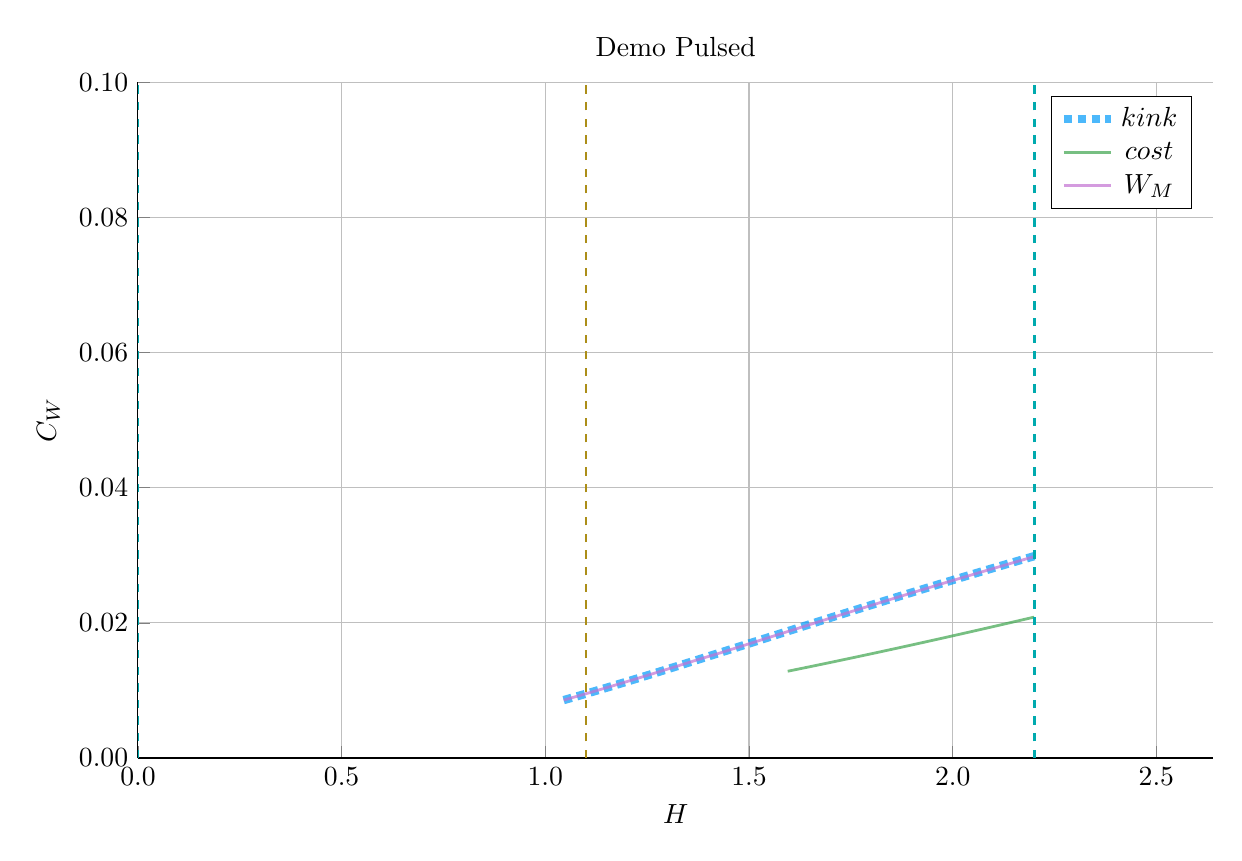
\begin{tikzpicture}[]
\begin{axis}[height = {101.6mm}, ylabel = {${C}_{W}$}, title = {Demo Pulsed}, xmin = {0.0}, xmax = {2.64}, ymax = {0.1}, xlabel = {${H}$}, {unbounded coords=jump, scaled x ticks = false, xticklabel style={rotate = 0}, xmajorgrids = true, xtick = {0.0,0.5,1.0,1.5,2.0,2.5}, xticklabels = {0.0,0.5,1.0,1.5,2.0,2.5}, xtick align = inside, axis lines* = left, scaled y ticks = false, yticklabel style={rotate = 0}, ymajorgrids = true, ytick = {0.0,0.02,0.04,0.06,0.08,0.1}, yticklabels = {0.00,0.02,0.04,0.06,0.08,0.10}, ytick align = inside, axis lines* = left,     xshift = 0.0mm,
    yshift = 0.0mm,
    axis background/.style={fill={rgb,1:red,1.00000000;green,1.00000000;blue,1.00000000}}
, colorbar style={title=}}, ymin = {0.0}, width = {152.4mm}]\addplot+ [color = {rgb,1:red,0.00000000;green,0.60560316;blue,0.97868012},
draw opacity=0.7,
line width=3,
dotted,mark = none,
mark size = 2.0,
mark options = {
    color = {rgb,1:red,0.00000000;green,0.00000000;blue,0.00000000}, draw opacity = 0.7,
    fill = {rgb,1:red,0.00000000;green,0.60560316;blue,0.97868012}, fill opacity = 0.7,
    line width = 1,
    rotate = 0,
    solid
}]coordinates {
(1.045, 0.008562900525474038)
(1.1, 0.009508186007059894)
(1.155, 0.010481303686531522)
(1.21, 0.011477221559201868)
(1.265, 0.012491405352808934)
(1.32, 0.013519771604802265)
(1.375, 0.01455865347279675)
(1.43, 0.01560476996557831)
(1.485, 0.01665520307882568)
(1.54, 0.01770736668237151)
(1.595, 0.018758981919712155)
(1.65, 0.019808050448382786)
(1.705, 0.020852828872326035)
(1.76, 0.02189180427909744)
(1.815, 0.022923671140831523)
(1.87, 0.023947309749696298)
(1.925, 0.024961766278888086)
(1.98, 0.0259662344951517)
(2.035, 0.02696003909922041)
(2.09, 0.02794262063490018)
(2.145, 0.028913521883941425)
(2.2, 0.029872378263278255)
};
\addlegendentry{$kink$}
\addplot+ [color = {rgb,1:red,0.24222430;green,0.64327509;blue,0.30444865},
draw opacity=0.7,
line width=1,
solid,mark = none,
mark size = 2.0,
mark options = {
    color = {rgb,1:red,0.00000000;green,0.00000000;blue,0.00000000}, draw opacity = 0.7,
    fill = {rgb,1:red,0.24222430;green,0.64327509;blue,0.30444865}, fill opacity = 0.7,
    line width = 1,
    rotate = 0,
    solid
}]coordinates {
(1.595, 0.012837618472183183)
(1.65, 0.01351605589807452)
(1.705, 0.014205803608469922)
(1.76, 0.014906425135137746)
(1.815, 0.015617503524478405)
(1.87, 0.016338645399656185)
(1.925, 0.01706942648235716)
(1.98, 0.017809426151890045)
(2.035, 0.018558272861644666)
(2.09, 0.019315572142598544)
(2.145, 0.02008091818544739)
(2.2, 0.02085393261082531)
};
\addlegendentry{$cost$}
\addplot+ [color = {rgb,1:red,0.76444018;green,0.44411178;blue,0.82429754},
draw opacity=0.7,
line width=1,
solid,mark = none,
mark size = 2.0,
mark options = {
    color = {rgb,1:red,0.00000000;green,0.00000000;blue,0.00000000}, draw opacity = 0.7,
    fill = {rgb,1:red,0.76444018;green,0.44411178;blue,0.82429754}, fill opacity = 0.7,
    line width = 1,
    rotate = 0,
    solid
}]coordinates {
(1.045, 0.008567863214519583)
(1.1, 0.009513323042301788)
(1.155, 0.010486539256799338)
(1.21, 0.011482480931373953)
(1.265, 0.012496617059929858)
(1.32, 0.013524867014744198)
(1.375, 0.014563566741331857)
(1.43, 0.015564622420606586)
(1.485, 0.01661309026146188)
(1.54, 0.01766334833375915)
(1.595, 0.01871311887654211)
(1.65, 0.019760403448633695)
(1.705, 0.020803458139051708)
(1.76, 0.02184076903618252)
(1.815, 0.022871029910387922)
(1.87, 0.023893118992242245)
(1.925, 0.024906081344326696)
(1.98, 0.025909109004890754)
(2.035, 0.02690152473392302)
(2.09, 0.027882767406153194)
(2.145, 0.02885237787071432)
(2.2, 0.029809986950531903)
};
\addlegendentry{$W_M$}
\addplot+ [color = {rgb,1:red,0.67554396;green,0.55566233;blue,0.09423434},
draw opacity=1.0,
line width=1,
dashed,mark = none,
mark size = 2.0,
mark options = {
    color = {rgb,1:red,0.00000000;green,0.00000000;blue,0.00000000}, draw opacity = 1.0,
    fill = {rgb,1:red,0.67554396;green,0.55566233;blue,0.09423434}, fill opacity = 1.0,
    line width = 1,
    rotate = 0,
    solid
},forget plot]coordinates {
(1.1, 0.0)
(1.1, 0.1)
};
\addplot+ [color = {rgb,1:red,0.00000048;green,0.66575898;blue,0.68099695},
draw opacity=1.0,
line width=1,
dashed,mark = none,
mark size = 2.0,
mark options = {
    color = {rgb,1:red,0.00000000;green,0.00000000;blue,0.00000000}, draw opacity = 1.0,
    fill = {rgb,1:red,0.00000048;green,0.66575898;blue,0.68099695}, fill opacity = 1.0,
    line width = 1,
    rotate = 0,
    solid
},forget plot]coordinates {
(0.0, 0.0)
(0.0, 0.1)
};
\addplot+ [color = {rgb,1:red,0.00000048;green,0.66575898;blue,0.68099695},
draw opacity=1.0,
line width=1,
dashed,mark = none,
mark size = 2.0,
mark options = {
    color = {rgb,1:red,0.00000000;green,0.00000000;blue,0.00000000}, draw opacity = 1.0,
    fill = {rgb,1:red,0.00000048;green,0.66575898;blue,0.68099695}, fill opacity = 1.0,
    line width = 1,
    rotate = 0,
    solid
},forget plot]coordinates {
(2.2, 0.0)
(2.2, 0.1)
};
\end{axis}

\end{tikzpicture}

		\end{adjustbox}
        \caption{Demo Pulsed Cost-per-Watt}
    \end{subfigure}
    \hfill \hfill ~\\ ~\\ ~\\ ~\\
    \hfill 
    \begin{subfigure}[t]{0.45\textwidth}
        \centering
		\begin{adjustbox}{width=\textwidth}
			\Large
			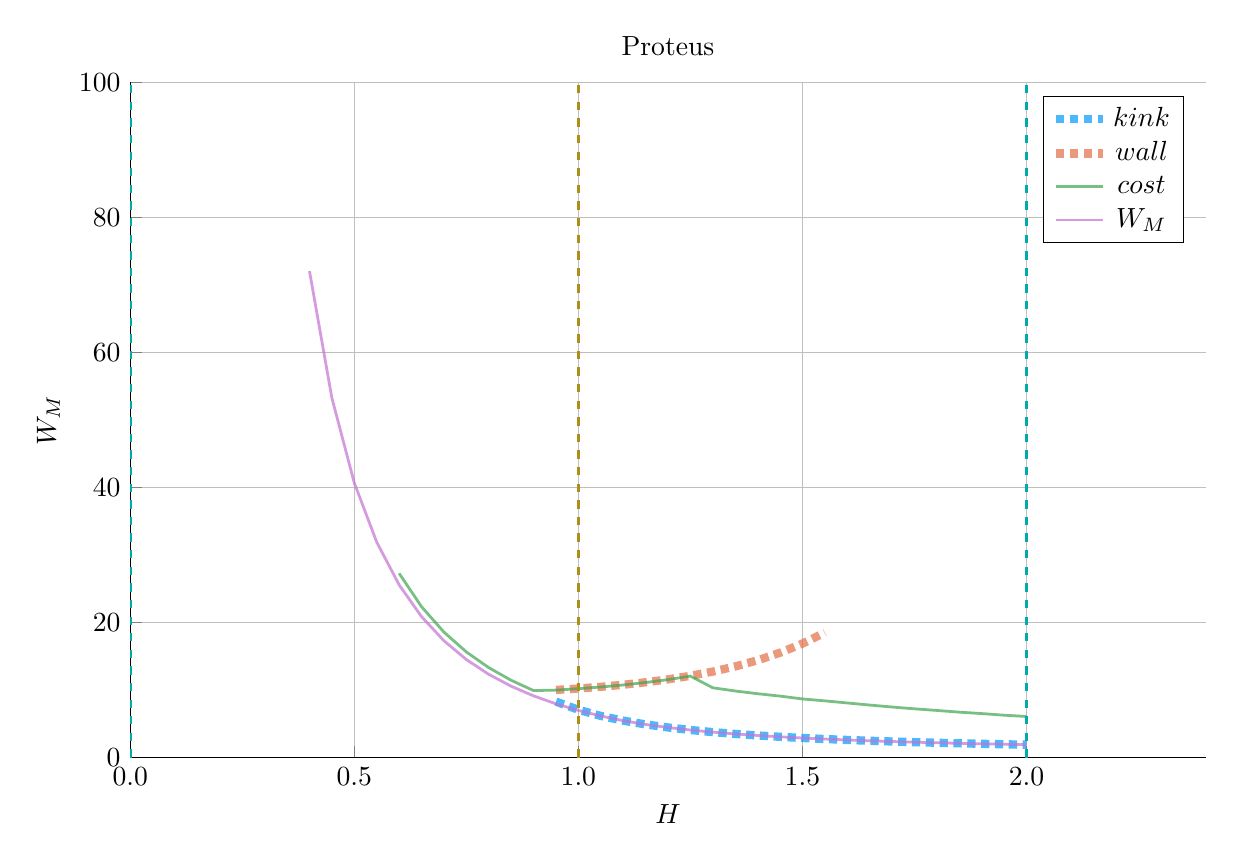
\begin{tikzpicture}[]
\begin{axis}[height = {101.6mm}, ylabel = {${W}_{M}$}, title = {Proteus}, xmin = {0.0}, xmax = {2.4}, ymax = {100.0}, xlabel = {${H}$}, {unbounded coords=jump, scaled x ticks = false, xticklabel style={rotate = 0}, xmajorgrids = true, xtick = {0.0,0.5,1.0,1.5,2.0}, xticklabels = {0.0,0.5,1.0,1.5,2.0}, xtick align = inside, axis lines* = left, scaled y ticks = false, yticklabel style={rotate = 0}, ymajorgrids = true, ytick = {0.0,20.0,40.0,60.0,80.0,100.0}, yticklabels = {0,20,40,60,80,100}, ytick align = inside, axis lines* = left,     xshift = 0.0mm,
    yshift = 0.0mm,
    axis background/.style={fill={rgb,1:red,1.00000000;green,1.00000000;blue,1.00000000}}
, colorbar style={title=}}, ymin = {0.0}, width = {152.4mm}]\addplot+ [color = {rgb,1:red,0.00000000;green,0.60560316;blue,0.97868012},
draw opacity=0.7,
line width=3,
dotted,mark = none,
mark size = 2.0,
mark options = {
    color = {rgb,1:red,0.00000000;green,0.00000000;blue,0.00000000}, draw opacity = 0.7,
    fill = {rgb,1:red,0.00000000;green,0.60560316;blue,0.97868012}, fill opacity = 0.7,
    line width = 1,
    rotate = 0,
    solid
}]coordinates {
(0.95, 8.296183844039575)
(1.0, 7.086769144908002)
(1.05, 6.181775721785971)
(1.1, 5.480949366373466)
(1.15, 4.923567135900637)
(1.2, 4.470692462177921)
(1.25, 4.096203887561972)
(1.3, 3.781933899884536)
(1.35, 3.5148629760075054)
(1.4, 3.2854236582043734)
(1.45, 3.086433169755101)
(1.5, 2.9123984603325805)
(1.55, 2.7590503991858912)
(1.6, 2.623023575982203)
(1.65, 2.5016312892415593)
(1.7, 2.392704302243594)
(1.75, 2.294473270577388)
(1.8, 2.2054816662324273)
(1.85, 2.1245203747463592)
(1.9, 2.050577940627468)
(1.95, 1.9828022746721614)
(2.0, 1.9204708676110047)
};
\addlegendentry{$kink$}
\addplot+ [color = {rgb,1:red,0.88887350;green,0.43564919;blue,0.27812294},
draw opacity=0.7,
line width=3,
dotted,mark = none,
mark size = 2.0,
mark options = {
    color = {rgb,1:red,0.00000000;green,0.00000000;blue,0.00000000}, draw opacity = 0.7,
    fill = {rgb,1:red,0.88887350;green,0.43564919;blue,0.27812294}, fill opacity = 0.7,
    line width = 1,
    rotate = 0,
    solid
}]coordinates {
(0.95, 10.024797897545305)
(1.0, 10.235766195929495)
(1.05, 10.488899487146755)
(1.1, 10.792220508626738)
(1.15, 11.155583907507257)
(1.2, 11.59113518979512)
(1.25, 12.11390937209129)
(1.3, 12.7426069957449)
(1.35, 13.500585565271978)
(1.4, 14.41707662205331)
(1.45, 15.528503875992053)
(1.5, 16.879217126464745)
(1.55, 18.518391800244235)
};
\addlegendentry{$wall$}
\addplot+ [color = {rgb,1:red,0.24222430;green,0.64327509;blue,0.30444865},
draw opacity=0.7,
line width=1,
solid,mark = none,
mark size = 2.0,
mark options = {
    color = {rgb,1:red,0.00000000;green,0.00000000;blue,0.00000000}, draw opacity = 0.7,
    fill = {rgb,1:red,0.24222430;green,0.64327509;blue,0.30444865}, fill opacity = 0.7,
    line width = 1,
    rotate = 0,
    solid
}]coordinates {
(0.6, 27.288407387481286)
(0.65, 22.353214318264936)
(0.7, 18.58662099411197)
(0.75, 15.652775301870053)
(0.8, 13.327232992105616)
(0.85, 11.455653248049614)
(0.9, 9.929237961369754)
(0.95, 9.999829968313627)
(1.0, 10.209283873179677)
(1.05, 10.460586375883373)
(1.1, 10.761688822197176)
(1.15, 11.122355391106282)
(1.2, 11.554615652339638)
(1.25, 12.073355976030422)
(1.3, 10.344173940091109)
(1.35, 9.869323307746308)
(1.4, 9.46482276601677)
(1.45, 9.114978686182061)
(1.5, 8.691786747556352)
(1.55, 8.409278897807058)
(1.6, 8.096934466381395)
(1.65, 7.789975454077516)
(1.7, 7.4959456967285645)
(1.75, 7.230113816710395)
(1.8, 6.989817608716943)
(1.85, 6.739134070201202)
(1.9, 6.527265957329837)
(1.95, 6.2841346987171605)
(2.0, 6.0958161232525665)
};
\addlegendentry{$cost$}
\addplot+ [color = {rgb,1:red,0.76444018;green,0.44411178;blue,0.82429754},
draw opacity=0.7,
line width=1,
solid,mark = none,
mark size = 2.0,
mark options = {
    color = {rgb,1:red,0.00000000;green,0.00000000;blue,0.00000000}, draw opacity = 0.7,
    fill = {rgb,1:red,0.76444018;green,0.44411178;blue,0.82429754}, fill opacity = 0.7,
    line width = 1,
    rotate = 0,
    solid
}]coordinates {
(0.4, 72.03178052102763)
(0.45, 53.23576620731215)
(0.5, 40.673388569316366)
(0.55, 31.91045571415749)
(0.6, 25.583005245105895)
(0.65, 20.881993779606706)
(0.7, 17.30564486911384)
(0.75, 14.528953468426364)
(0.8, 12.335297009669484)
(0.85, 10.575816011821674)
(0.9, 9.145463815576935)
(0.95, 7.969061443373584)
(1.0, 6.991275094865506)
(1.05, 6.170456951860706)
(1.1, 5.471837294898814)
(1.15, 4.916064964372644)
(1.2, 4.464401308044445)
(1.25, 4.090848888293192)
(1.3, 3.7773186041717763)
(1.35, 3.5108430536736326)
(1.4, 3.281890559671486)
(1.45, 3.083303583025399)
(1.5, 2.909607292188191)
(1.55, 2.756546032188435)
(1.6, 2.620573165427533)
(1.65, 2.4991743461601748)
(1.7, 2.390247946407766)
(1.75, 2.292022826965956)
(1.8, 2.2030410998030234)
(1.85, 2.1220926426292905)
(1.9, 2.048165205240727)
(1.95, 1.980406132168879)
(2.0, 1.918092444652833)
};
\addlegendentry{$W_M$}
\addplot+ [color = {rgb,1:red,0.67554396;green,0.55566233;blue,0.09423434},
draw opacity=1.0,
line width=1,
dashed,mark = none,
mark size = 2.0,
mark options = {
    color = {rgb,1:red,0.00000000;green,0.00000000;blue,0.00000000}, draw opacity = 1.0,
    fill = {rgb,1:red,0.67554396;green,0.55566233;blue,0.09423434}, fill opacity = 1.0,
    line width = 1,
    rotate = 0,
    solid
},forget plot]coordinates {
(1.0, 0.0)
(1.0, 100.0)
};
\addplot+ [color = {rgb,1:red,0.00000048;green,0.66575898;blue,0.68099695},
draw opacity=1.0,
line width=1,
dashed,mark = none,
mark size = 2.0,
mark options = {
    color = {rgb,1:red,0.00000000;green,0.00000000;blue,0.00000000}, draw opacity = 1.0,
    fill = {rgb,1:red,0.00000048;green,0.66575898;blue,0.68099695}, fill opacity = 1.0,
    line width = 1,
    rotate = 0,
    solid
},forget plot]coordinates {
(0.0, 0.0)
(0.0, 100.0)
};
\addplot+ [color = {rgb,1:red,0.00000048;green,0.66575898;blue,0.68099695},
draw opacity=1.0,
line width=1,
dashed,mark = none,
mark size = 2.0,
mark options = {
    color = {rgb,1:red,0.00000000;green,0.00000000;blue,0.00000000}, draw opacity = 1.0,
    fill = {rgb,1:red,0.00000048;green,0.66575898;blue,0.68099695}, fill opacity = 1.0,
    line width = 1,
    rotate = 0,
    solid
},forget plot]coordinates {
(2.0, 0.0)
(2.0, 100.0)
};
\end{axis}

\end{tikzpicture}

		\end{adjustbox}
        \caption{Proteus Capital Cost}
    \end{subfigure}
    \hfill
    \begin{subfigure}[t]{0.45\textwidth}
        \centering
		\begin{adjustbox}{width=\textwidth}
			\Large
			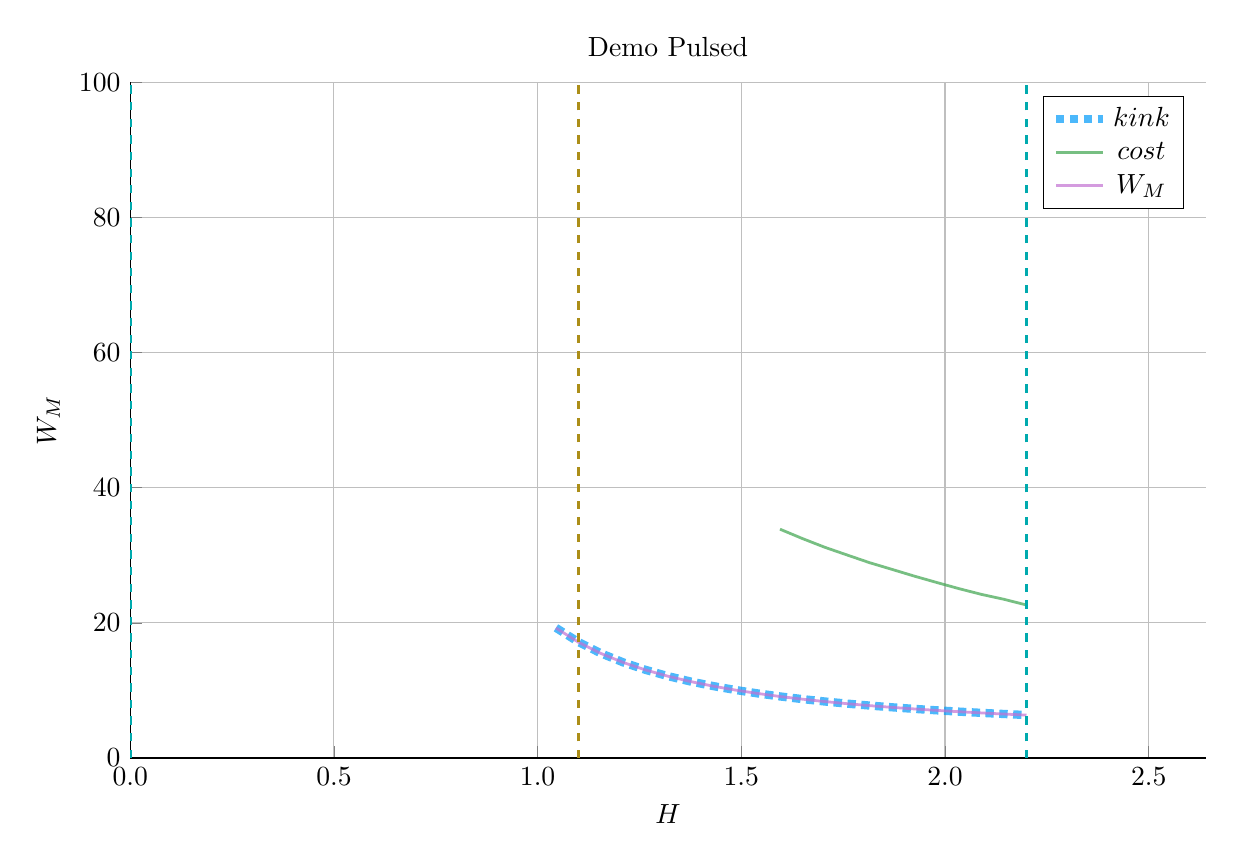
\begin{tikzpicture}[]
\begin{axis}[height = {101.6mm}, ylabel = {${W}_{M}$}, title = {Demo Pulsed}, xmin = {0.0}, xmax = {2.64}, ymax = {100.0}, xlabel = {${H}$}, {unbounded coords=jump, scaled x ticks = false, xticklabel style={rotate = 0}, xmajorgrids = true, xtick = {0.0,0.5,1.0,1.5,2.0,2.5}, xticklabels = {0.0,0.5,1.0,1.5,2.0,2.5}, xtick align = inside, axis lines* = left, scaled y ticks = false, yticklabel style={rotate = 0}, ymajorgrids = true, ytick = {0.0,20.0,40.0,60.0,80.0,100.0}, yticklabels = {0,20,40,60,80,100}, ytick align = inside, axis lines* = left,     xshift = 0.0mm,
    yshift = 0.0mm,
    axis background/.style={fill={rgb,1:red,1.00000000;green,1.00000000;blue,1.00000000}}
, colorbar style={title=}}, ymin = {0.0}, width = {152.4mm}]\addplot+ [color = {rgb,1:red,0.00000000;green,0.60560316;blue,0.97868012},
draw opacity=0.7,
line width=3,
dotted,mark = none,
mark size = 2.0,
mark options = {
    color = {rgb,1:red,0.00000000;green,0.00000000;blue,0.00000000}, draw opacity = 0.7,
    fill = {rgb,1:red,0.00000000;green,0.60560316;blue,0.97868012}, fill opacity = 0.7,
    line width = 1,
    rotate = 0,
    solid
}]coordinates {
(1.045, 19.266036575091096)
(1.1, 17.166473566094577)
(1.155, 15.5019442407049)
(1.21, 14.153966782219351)
(1.265, 13.042936912510411)
(1.32, 12.113471642815448)
(1.375, 11.325909627415403)
(1.43, 10.651146390371457)
(1.485, 10.06737684757331)
(1.54, 9.55796365667095)
(1.595, 9.110010367825117)
(1.65, 8.713378468404333)
(1.705, 8.35999688264097)
(1.76, 8.043367452396877)
(1.815, 7.758204726005019)
(1.87, 7.500169552604314)
(1.925, 7.265669320970731)
(1.98, 7.051706282910641)
(2.035, 6.855761060829623)
(2.09, 6.675702232904676)
(2.145, 6.509715475260026)
(2.2, 6.356247978269343)
};
\addlegendentry{$kink$}
\addplot+ [color = {rgb,1:red,0.24222430;green,0.64327509;blue,0.30444865},
draw opacity=0.7,
line width=1,
solid,mark = none,
mark size = 2.0,
mark options = {
    color = {rgb,1:red,0.00000000;green,0.00000000;blue,0.00000000}, draw opacity = 0.7,
    fill = {rgb,1:red,0.24222430;green,0.64327509;blue,0.30444865}, fill opacity = 0.7,
    line width = 1,
    rotate = 0,
    solid
}]coordinates {
(1.595, 33.86772395124183)
(1.65, 32.48229097350921)
(1.705, 31.188301761541396)
(1.76, 30.042407894531546)
(1.815, 28.907311828796562)
(1.87, 27.917272999401945)
(1.925, 26.914825706659318)
(1.98, 25.973854740340027)
(2.035, 25.055352661147893)
(2.09, 24.20869371627589)
(2.145, 23.486616271247453)
(2.2, 22.643825907165436)
};
\addlegendentry{$cost$}
\addplot+ [color = {rgb,1:red,0.76444018;green,0.44411178;blue,0.82429754},
draw opacity=0.7,
line width=1,
solid,mark = none,
mark size = 2.0,
mark options = {
    color = {rgb,1:red,0.00000000;green,0.00000000;blue,0.00000000}, draw opacity = 0.7,
    fill = {rgb,1:red,0.76444018;green,0.44411178;blue,0.82429754}, fill opacity = 0.7,
    line width = 1,
    rotate = 0,
    solid
}]coordinates {
(1.045, 19.237500181392328)
(1.1, 17.143413996744133)
(1.155, 15.482916466996478)
(1.21, 14.1379978901947)
(1.265, 13.029348174735949)
(1.32, 12.101773846314275)
(1.375, 11.315740182760772)
(1.43, 10.641073307955129)
(1.485, 10.057210081145517)
(1.54, 9.547752855086221)
(1.595, 9.09979093866626)
(1.65, 8.703175655201754)
(1.705, 8.349828669604108)
(1.76, 8.03324655329132)
(1.815, 7.748140118900301)
(1.87, 7.490167271524911)
(1.925, 7.255733405969062)
(1.98, 7.0418392185328775)
(2.035, 6.845964150321039)
(2.09, 6.665975947441873)
(2.145, 6.500059632778603)
(2.2, 6.346661457133039)
};
\addlegendentry{$W_M$}
\addplot+ [color = {rgb,1:red,0.67554396;green,0.55566233;blue,0.09423434},
draw opacity=1.0,
line width=1,
dashed,mark = none,
mark size = 2.0,
mark options = {
    color = {rgb,1:red,0.00000000;green,0.00000000;blue,0.00000000}, draw opacity = 1.0,
    fill = {rgb,1:red,0.67554396;green,0.55566233;blue,0.09423434}, fill opacity = 1.0,
    line width = 1,
    rotate = 0,
    solid
},forget plot]coordinates {
(1.1, 0.0)
(1.1, 100.0)
};
\addplot+ [color = {rgb,1:red,0.00000048;green,0.66575898;blue,0.68099695},
draw opacity=1.0,
line width=1,
dashed,mark = none,
mark size = 2.0,
mark options = {
    color = {rgb,1:red,0.00000000;green,0.00000000;blue,0.00000000}, draw opacity = 1.0,
    fill = {rgb,1:red,0.00000048;green,0.66575898;blue,0.68099695}, fill opacity = 1.0,
    line width = 1,
    rotate = 0,
    solid
},forget plot]coordinates {
(0.0, 0.0)
(0.0, 100.0)
};
\addplot+ [color = {rgb,1:red,0.00000048;green,0.66575898;blue,0.68099695},
draw opacity=1.0,
line width=1,
dashed,mark = none,
mark size = 2.0,
mark options = {
    color = {rgb,1:red,0.00000000;green,0.00000000;blue,0.00000000}, draw opacity = 1.0,
    fill = {rgb,1:red,0.00000048;green,0.66575898;blue,0.68099695}, fill opacity = 1.0,
    line width = 1,
    rotate = 0,
    solid
},forget plot]coordinates {
(2.2, 0.0)
(2.2, 100.0)
};
\end{axis}

\end{tikzpicture}

		\end{adjustbox}
        \caption{Demo Pulsed Capital Cost}
    \end{subfigure}	
    \hfill \hfill ~\\ ~\\ ~\\
    \hfill 
    \begin{subfigure}[t]{0.45\textwidth}
        \centering
		\begin{adjustbox}{width=\textwidth}
			\Large
			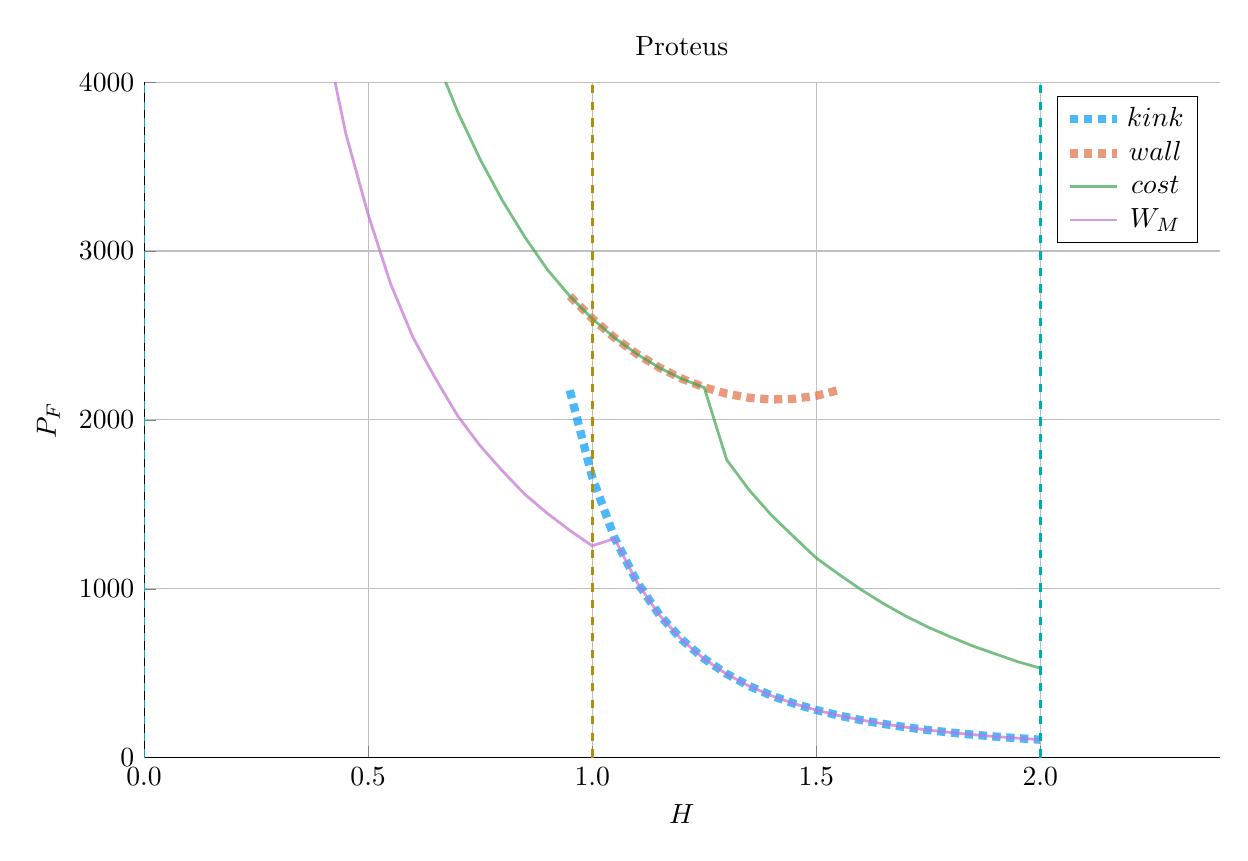
\begin{tikzpicture}[]
\begin{axis}[height = {101.6mm}, ylabel = {${P}_{F}$}, title = {Proteus}, xmin = {0.0}, xmax = {2.4}, ymax = {4000.0}, xlabel = {${H}$}, {unbounded coords=jump, scaled x ticks = false, xticklabel style={rotate = 0}, xmajorgrids = true, xtick = {0.0,0.5,1.0,1.5,2.0}, xticklabels = {0.0,0.5,1.0,1.5,2.0}, xtick align = inside, axis lines* = left, scaled y ticks = false, yticklabel style={rotate = 0}, ymajorgrids = true, ytick = {0.0,1000.0,2000.0,3000.0,4000.0}, yticklabels = {0,1000,2000,3000,4000}, ytick align = inside, axis lines* = left,     xshift = 0.0mm,
    yshift = 0.0mm,
    axis background/.style={fill={rgb,1:red,1.00000000;green,1.00000000;blue,1.00000000}}
, colorbar style={title=}}, ymin = {0.0}, width = {152.4mm}]\addplot+ [color = {rgb,1:red,0.00000000;green,0.60560316;blue,0.97868012},
draw opacity=0.7,
line width=3,
dotted,mark = none,
mark size = 2.0,
mark options = {
    color = {rgb,1:red,0.00000000;green,0.00000000;blue,0.00000000}, draw opacity = 0.7,
    fill = {rgb,1:red,0.00000000;green,0.60560316;blue,0.97868012}, fill opacity = 0.7,
    line width = 1,
    rotate = 0,
    solid
}]coordinates {
(0.95, 2175.5296002700434)
(1.0, 1661.3577869805065)
(1.05, 1300.6958472635408)
(1.1, 1039.7100194871657)
(1.15, 845.9533255882448)
(1.2, 698.9624784313035)
(1.25, 585.3529598336329)
(1.3, 496.1022398747714)
(1.35, 424.9704216769565)
(1.4, 367.5454816762811)
(1.45, 320.6467048930754)
(1.5, 281.9412485038502)
(1.55, 249.6915599475339)
(1.6, 222.5853492231558)
(1.65, 199.61890582244618)
(1.7, 180.0156238031778)
(1.75, 163.1682121986067)
(1.8, 148.59711540167376)
(1.85, 135.9202024934991)
(1.9, 124.83040357039394)
(1.95, 115.07902467792957)
(2.0, 106.46317010408701)
};
\addlegendentry{$kink$}
\addplot+ [color = {rgb,1:red,0.88887350;green,0.43564919;blue,0.27812294},
draw opacity=0.7,
line width=3,
dotted,mark = none,
mark size = 2.0,
mark options = {
    color = {rgb,1:red,0.00000000;green,0.00000000;blue,0.00000000}, draw opacity = 0.7,
    fill = {rgb,1:red,0.88887350;green,0.43564919;blue,0.27812294}, fill opacity = 0.7,
    line width = 1,
    rotate = 0,
    solid
}]coordinates {
(0.95, 2733.826896193781)
(1.0, 2600.4697515783337)
(1.05, 2486.619987468522)
(1.1, 2390.252493826267)
(1.15, 2309.8530327858357)
(1.2, 2244.329946710276)
(1.25, 2192.9523032793136)
(1.3, 2155.3071239500264)
(1.35, 2131.2694155117288)
(1.4, 2120.9769238379035)
(1.45, 2124.7924256842894)
(1.5, 2143.202004913529)
(1.55, 2176.450311775978)
};
\addlegendentry{$wall$}
\addplot+ [color = {rgb,1:red,0.24222430;green,0.64327509;blue,0.30444865},
draw opacity=0.7,
line width=1,
solid,mark = none,
mark size = 2.0,
mark options = {
    color = {rgb,1:red,0.00000000;green,0.00000000;blue,0.00000000}, draw opacity = 0.7,
    fill = {rgb,1:red,0.24222430;green,0.64327509;blue,0.30444865}, fill opacity = 0.7,
    line width = 1,
    rotate = 0,
    solid
}]coordinates {
(0.6, 4533.65313644835)
(0.65, 4150.331179531389)
(0.7, 3824.0867742458104)
(0.75, 3542.797263824155)
(0.8, 3297.559000708419)
(0.85, 3081.683508296413)
(0.9, 2890.0475153750854)
(0.95, 2733.495699622131)
(1.0, 2600.0006699519377)
(1.05, 2486.0008281085816)
(1.1, 2389.4679503499774)
(1.15, 2308.8842483162302)
(1.2, 2243.1539283144857)
(1.25, 2191.54120292087)
(1.3, 1764.3060418646296)
(1.35, 1585.5890526138944)
(1.4, 1435.5414455426135)
(1.45, 1307.8946353270621)
(1.5, 1182.2158202599155)
(1.55, 1086.2442883296173)
(1.6, 995.0125095090548)
(1.65, 912.221879942583)
(1.7, 837.7776562823368)
(1.75, 772.3757205298201)
(1.8, 714.7297928727821)
(1.85, 660.4745462751914)
(1.9, 613.9201827620487)
(1.95, 567.9186226009322)
(2.0, 529.9531309338922)
};
\addlegendentry{$cost$}
\addplot+ [color = {rgb,1:red,0.76444018;green,0.44411178;blue,0.82429754},
draw opacity=0.7,
line width=1,
solid,mark = none,
mark size = 2.0,
mark options = {
    color = {rgb,1:red,0.00000000;green,0.00000000;blue,0.00000000}, draw opacity = 0.7,
    fill = {rgb,1:red,0.76444018;green,0.44411178;blue,0.82429754}, fill opacity = 0.7,
    line width = 1,
    rotate = 0,
    solid
}]coordinates {
(0.4, 4332.867335366913)
(0.45, 3697.5892079740934)
(0.5, 3216.758140128481)
(0.55, 2806.281853810256)
(0.6, 2488.9302872893472)
(0.65, 2246.2900365923156)
(0.7, 2023.4050737919029)
(0.75, 1846.7546225582166)
(0.8, 1696.4767174580222)
(0.85, 1558.8369460915019)
(0.9, 1446.598764089886)
(0.95, 1345.8283280045227)
(1.0, 1254.3719976750003)
(1.05, 1297.4499743830818)
(1.1, 1037.2793481789427)
(1.15, 844.092090451781)
(1.2, 697.5103218794108)
(1.25, 584.2017421885754)
(1.3, 495.17689757150174)
(1.35, 424.21758791870303)
(1.4, 366.926421795714)
(1.45, 320.1327888364858)
(1.5, 281.5109701980368)
(1.55, 249.32853697811342)
(1.6, 223.01371643430133)
(1.65, 199.98787916871922)
(1.7, 180.33533919625512)
(1.75, 163.44676794664525)
(1.8, 148.8410410835442)
(1.85, 136.13480383980067)
(1.9, 125.02002697524327)
(1.95, 115.24725227887417)
(2.0, 106.61297617106092)
};
\addlegendentry{$W_M$}
\addplot+ [color = {rgb,1:red,0.67554396;green,0.55566233;blue,0.09423434},
draw opacity=1.0,
line width=1,
dashed,mark = none,
mark size = 2.0,
mark options = {
    color = {rgb,1:red,0.00000000;green,0.00000000;blue,0.00000000}, draw opacity = 1.0,
    fill = {rgb,1:red,0.67554396;green,0.55566233;blue,0.09423434}, fill opacity = 1.0,
    line width = 1,
    rotate = 0,
    solid
},forget plot]coordinates {
(1.0, 0.0)
(1.0, 4000.0)
};
\addplot+ [color = {rgb,1:red,0.00000048;green,0.66575898;blue,0.68099695},
draw opacity=1.0,
line width=1,
dashed,mark = none,
mark size = 2.0,
mark options = {
    color = {rgb,1:red,0.00000000;green,0.00000000;blue,0.00000000}, draw opacity = 1.0,
    fill = {rgb,1:red,0.00000048;green,0.66575898;blue,0.68099695}, fill opacity = 1.0,
    line width = 1,
    rotate = 0,
    solid
},forget plot]coordinates {
(0.0, 0.0)
(0.0, 4000.0)
};
\addplot+ [color = {rgb,1:red,0.00000048;green,0.66575898;blue,0.68099695},
draw opacity=1.0,
line width=1,
dashed,mark = none,
mark size = 2.0,
mark options = {
    color = {rgb,1:red,0.00000000;green,0.00000000;blue,0.00000000}, draw opacity = 1.0,
    fill = {rgb,1:red,0.00000048;green,0.66575898;blue,0.68099695}, fill opacity = 1.0,
    line width = 1,
    rotate = 0,
    solid
},forget plot]coordinates {
(2.0, 0.0)
(2.0, 4000.0)
};
\end{axis}

\end{tikzpicture}

		\end{adjustbox}
        \caption{Proteus Fusion Power}
    \end{subfigure}
    \hfill
    \begin{subfigure}[t]{0.45\textwidth}
        \centering
		\begin{adjustbox}{width=\textwidth}
			\Large
			\begin{tikzpicture}[]
\begin{axis}[height = {101.6mm}, ylabel = {${P}_{F}$}, title = {Demo Pulsed}, xmin = {0.0}, xmax = {2.64}, ymax = {4000.0}, xlabel = {${H}$}, {unbounded coords=jump, scaled x ticks = false, xticklabel style={rotate = 0}, xmajorgrids = true, xtick = {0.0,0.5,1.0,1.5,2.0,2.5}, xticklabels = {0.0,0.5,1.0,1.5,2.0,2.5}, xtick align = inside, axis lines* = left, scaled y ticks = false, yticklabel style={rotate = 0}, ymajorgrids = true, ytick = {0.0,1000.0,2000.0,3000.0,4000.0}, yticklabels = {0,1000,2000,3000,4000}, ytick align = inside, axis lines* = left,     xshift = 0.0mm,
    yshift = 0.0mm,
    axis background/.style={fill={rgb,1:red,1.00000000;green,1.00000000;blue,1.00000000}}
, colorbar style={title=}}, ymin = {0.0}, width = {152.4mm}]\addplot+ [color = {rgb,1:red,0.00000000;green,0.60560316;blue,0.97868012},
draw opacity=0.7,
line width=3,
dotted,mark = none,
mark size = 2.0,
mark options = {
    color = {rgb,1:red,0.00000000;green,0.00000000;blue,0.00000000}, draw opacity = 0.7,
    fill = {rgb,1:red,0.00000000;green,0.60560316;blue,0.97868012}, fill opacity = 0.7,
    line width = 1,
    rotate = 0,
    solid
}]coordinates {
(1.045, 2249.942822268689)
(1.1, 1805.4414957120475)
(1.155, 1479.009167592854)
(1.21, 1233.2224057199105)
(1.265, 1044.1528830523025)
(1.32, 895.9819734316151)
(1.375, 777.9503543083968)
(1.43, 682.5570908040443)
(1.485, 604.458366549268)
(1.54, 539.7732948166899)
(1.595, 485.63458330604885)
(1.65, 439.8907651770308)
(1.705, 400.90468942252687)
(1.76, 367.41455157612484)
(1.815, 338.4363995776464)
(1.87, 313.1946607363456)
(1.925, 291.0719233484618)
(1.98, 271.5721559176131)
(2.035, 254.29343910068246)
(2.09, 238.9075212425409)
(2.145, 225.1443287120108)
(2.2, 212.78011152138495)
};
\addlegendentry{$kink$}
\addplot+ [color = {rgb,1:red,0.24222430;green,0.64327509;blue,0.30444865},
draw opacity=0.7,
line width=1,
solid,mark = none,
mark size = 2.0,
mark options = {
    color = {rgb,1:red,0.00000000;green,0.00000000;blue,0.00000000}, draw opacity = 0.7,
    fill = {rgb,1:red,0.24222430;green,0.64327509;blue,0.30444865}, fill opacity = 0.7,
    line width = 1,
    rotate = 0,
    solid
}]coordinates {
(1.595, 2638.1625240403514)
(1.65, 2403.2373954695313)
(1.705, 2195.461983083168)
(1.76, 2015.3999112580614)
(1.815, 1850.9559984083314)
(1.87, 1708.6650892117048)
(1.925, 1576.7855899832543)
(1.98, 1458.4329960335933)
(2.035, 1350.0907572563542)
(2.09, 1253.3252205812769)
(2.145, 1169.598723243052)
(2.2, 1085.8300124845991)
};
\addlegendentry{$cost$}
\addplot+ [color = {rgb,1:red,0.76444018;green,0.44411178;blue,0.82429754},
draw opacity=0.7,
line width=1,
solid,mark = none,
mark size = 2.0,
mark options = {
    color = {rgb,1:red,0.00000000;green,0.00000000;blue,0.00000000}, draw opacity = 0.7,
    fill = {rgb,1:red,0.76444018;green,0.44411178;blue,0.82429754}, fill opacity = 0.7,
    line width = 1,
    rotate = 0,
    solid
}]coordinates {
(1.045, 2245.3089760806847)
(1.1, 1802.042663800494)
(1.155, 1476.4562538549171)
(1.21, 1231.266829415322)
(1.265, 1042.6300263704393)
(1.32, 894.7795074895353)
(1.375, 776.9896196270621)
(1.43, 683.670507410897)
(1.485, 605.3786455657603)
(1.54, 540.5403706407146)
(1.595, 486.27869029749667)
(1.65, 440.4351195472946)
(1.705, 401.3673406504483)
(1.76, 367.80969296378885)
(1.815, 338.77530435921165)
(1.87, 313.48637546888966)
(1.925, 291.32376569635795)
(1.98, 271.7900958000377)
(2.035, 254.48238410398454)
(2.09, 239.07153297741957)
(2.145, 225.28679133154847)
(2.2, 212.90386566304065)
};
\addlegendentry{$W_M$}
\addplot+ [color = {rgb,1:red,0.67554396;green,0.55566233;blue,0.09423434},
draw opacity=1.0,
line width=1,
dashed,mark = none,
mark size = 2.0,
mark options = {
    color = {rgb,1:red,0.00000000;green,0.00000000;blue,0.00000000}, draw opacity = 1.0,
    fill = {rgb,1:red,0.67554396;green,0.55566233;blue,0.09423434}, fill opacity = 1.0,
    line width = 1,
    rotate = 0,
    solid
},forget plot]coordinates {
(1.1, 0.0)
(1.1, 4000.0)
};
\addplot+ [color = {rgb,1:red,0.00000048;green,0.66575898;blue,0.68099695},
draw opacity=1.0,
line width=1,
dashed,mark = none,
mark size = 2.0,
mark options = {
    color = {rgb,1:red,0.00000000;green,0.00000000;blue,0.00000000}, draw opacity = 1.0,
    fill = {rgb,1:red,0.00000048;green,0.66575898;blue,0.68099695}, fill opacity = 1.0,
    line width = 1,
    rotate = 0,
    solid
},forget plot]coordinates {
(0.0, 0.0)
(0.0, 4000.0)
};
\addplot+ [color = {rgb,1:red,0.00000048;green,0.66575898;blue,0.68099695},
draw opacity=1.0,
line width=1,
dashed,mark = none,
mark size = 2.0,
mark options = {
    color = {rgb,1:red,0.00000000;green,0.00000000;blue,0.00000000}, draw opacity = 1.0,
    fill = {rgb,1:red,0.00000048;green,0.66575898;blue,0.68099695}, fill opacity = 1.0,
    line width = 1,
    rotate = 0,
    solid
},forget plot]coordinates {
(2.2, 0.0)
(2.2, 4000.0)
};
\end{axis}

\end{tikzpicture}

		\end{adjustbox}
        \caption{Demo Pulsed Fusion Power}
    \end{subfigure}	
    \hfill \hfill ~\\ ~\\ ~\\
    \caption{Pulsed H Sensitivities}
    \label{fig:pulsed_h}
\end{figure*}

\subsubsection{Showcasing the Current Drive Efficiency}

The last exploration is less about building an efficient machine and more about understanding the self-consistent current drive efficiency in steady-state tokamaks. Using the Ehst-Karney model \cite{ehstkarney} coupled with Jeff's textbook \cite{jeff} leads to a remarkably simple and accurate solver. The model captures the physics almost spot on for the different designs.\footnote{ It did, however, not converge for the DEMO steady reactor. This is probably due to lack of self-consistency for $\eta_{CD}$ in their systems framework. }

\begin{figure*}
    \centering
    \hfill 
    \begin{subfigure}[t]{0.45\textwidth}
        \centering
		\begin{adjustbox}{width=\textwidth}
			\Large
			\begin{tikzpicture}[]
\begin{axis}[height = {101.6mm}, ylabel = {${\eta}_{CD}$}, title = {Charybdis}, xmin = {0.0}, xmax = {20.0}, ymax = {0.4}, xlabel = {${B}_{0}$}, {unbounded coords=jump, scaled x ticks = false, xticklabel style={rotate = 0}, xmajorgrids = true, xtick = {0.0,5.0,10.0,15.0,20.0}, xticklabels = {0,5,10,15,20}, xtick align = inside, axis lines* = left, scaled y ticks = false, yticklabel style={rotate = 0}, ymajorgrids = true, ytick = {0.0,0.1,0.2,0.30000000000000004,0.4}, yticklabels = {0.0,0.1,0.2,0.3,0.4}, ytick align = inside, axis lines* = left,     xshift = 0.0mm,
    yshift = 0.0mm,
    axis background/.style={fill={rgb,1:red,1.00000000;green,1.00000000;blue,1.00000000}}
, colorbar style={title=}}, ymin = {0.0}, width = {152.4mm}]\addplot+ [color = {rgb,1:red,0.00000000;green,0.60560316;blue,0.97868012},
draw opacity=1.0,
line width=1,
solid,mark = none,
mark size = 2.0,
mark options = {
    color = {rgb,1:red,0.00000000;green,0.00000000;blue,0.00000000}, draw opacity = 1.0,
    fill = {rgb,1:red,0.00000000;green,0.60560316;blue,0.97868012}, fill opacity = 1.0,
    line width = 1,
    rotate = 0,
    solid
}]coordinates {
(10.112818033153026, 0.2890124001708679)
(9.722156888543116, 0.2890934058074779)
(9.357875603858393, 0.28916957864023385)
(9.017653755630063, 0.289241971718532)
(8.6995124437054, 0.2893093526110478)
(8.401566530516865, 0.28937346296062694)
(8.122163706328223, 0.2894349713924345)
(7.859819415455661, 0.28949448265460487)
(7.613196557650265, 0.28955254309932243)
(7.381088038653343, 0.2896096457184144)
(7.162401716104116, 0.28966623476343445)
(6.956147367527331, 0.2897227099799709)
(6.761425371986388, 0.28977943048511107)
(6.577416849463348, 0.28983671831577723)
(6.403375044688587, 0.28989486167423906)
(6.2386177769852695, 0.2899541178955051)
(6.0825208065966905, 0.2900147161612859)
(5.934511989185341, 0.2900768599723193)
(5.794066116682695, 0.29014072942323216)
(5.660700347012839, 0.29020648326562526)
(5.533970150598111, 0.2902742608008287)
(5.413465705416883, 0.2903441836068744)
(5.298808685607224, 0.2904163571218577)
(5.189649392059402, 0.29049087208037166)
(5.085664187259174, 0.2905678058370994)
(4.986553195072601, 0.29064722357133665)
(4.892038235455667, 0.29072917938928644)
(4.801860966679364, 0.29081371733194217)
(4.7157812114040425, 0.2909008722967884)
(4.633575445956479, 0.2909906708807873)
(4.5550354347559185, 0.29108313215149306)
(4.479966994069385, 0.29117826835249444)
(4.408188871204256, 0.29127608554886664)
(4.33953172691477, 0.2913765842177861)
(4.273837210246432, 0.2914797597890203)
(4.210957116299974, 0.2915856031395779)
(4.15075261849161, 0.2916941010464348)
(4.0930935678432965, 0.2918052366009017)
(4.037857852672517, 0.29191898958788354)
(3.9849308127842145, 0.29203533683300315)
(3.9342047029103653, 0.29215425252029686)
(3.8855782007091695, 0.2922757084829535)
(3.838955955133626, 0.2923996744693585)
(3.7942481714200484, 0.29252611838650283)
(3.7513702293348077, 0.29265500652264587)
(3.710242331663442, 0.29278630375095266)
(3.6707891802306123, 0.2929199737156832)
(3.6329396770109583, 0.2930559790023756)
(3.5966266481325166, 0.2931942812933425)
(3.5617865887889004, 0.2933348415096877)
(3.5283594272686503, 0.29347761994094823)
(3.496288306480746, 0.2936225763633821)
(3.465519381509793, 0.2937696701478163)
(3.4360016318699595, 0.2939188603579226)
(3.4076866872513096, 0.29407010583968624)
(3.380528665662031, 0.2942233653027989)
(3.3544840229690007, 0.2943785973946173)
(3.3295114129297314, 0.29453576076730204)
(3.3055715568879336, 0.2946948141386861)
(3.2826271223788512, 0.2948557163473816)
(3.260642607548369, 0.29501842638145964)
(3.239584247604666, 0.29518290352905774)
(3.2194198921826622, 0.29534910720753893)
(3.2001189373344725, 0.29551699721118)
(3.181652227422265, 0.2956865336381098)
(3.163991977015565, 0.2958576769405733)
(3.1471116955378684, 0.29603038795087755)
(3.130986116696265, 0.2962046279044162)
(3.115591132350856, 0.2963803584600108)
(3.1009037305081053, 0.29655754171778737)
(3.0869019371473265, 0.2967361402347924)
(3.0735647616124355, 0.2969161170385373)
(3.0608721453218655, 0.2970974356386405)
};
\addlegendentry{Steady - Beta}
\addplot+ [color = {rgb,1:red,0.88887350;green,0.43564919;blue,0.27812294},
draw opacity=1.0,
line width=1,
solid,mark = none,
mark size = 2.0,
mark options = {
    color = {rgb,1:red,0.00000000;green,0.00000000;blue,0.00000000}, draw opacity = 1.0,
    fill = {rgb,1:red,0.88887350;green,0.43564919;blue,0.27812294}, fill opacity = 1.0,
    line width = 1,
    rotate = 0,
    solid
}]coordinates {
(20.758867641064707, 0.550619788361201)
(20.346250098246923, 0.5079685190808274)
(19.57104597888471, 0.47503902985770124)
(18.681781921115476, 0.44813959090357636)
(17.775790175980152, 0.4255015286239918)
(16.896654716492492, 0.406077367741247)
(16.063927450323227, 0.3891772930411093)
(15.285557510665852, 0.3743136422319958)
(14.563500533069154, 0.36112607873138414)
(13.896568848875791, 0.349339912602884)
(13.281970890030232, 0.33874072709065145)
(12.716170469467318, 0.32915795214509086)
(12.195372283741088, 0.32045374568641577)
(11.715794270833433, 0.3125152089271154)
(11.273815669498969, 0.3052487883586615)
(10.866051794088186, 0.29857616101982265)
(10.489365023931143, 0.2924314183330621)
};
\addlegendentry{Steady - Wall}
\addplot+ [color = {rgb,1:red,0.24222430;green,0.64327509;blue,0.30444865},
draw opacity=1.0,
line width=1,
dashed,mark = none,
mark size = 2.0,
mark options = {
    color = {rgb,1:red,0.00000000;green,0.00000000;blue,0.00000000}, draw opacity = 1.0,
    fill = {rgb,1:red,0.24222430;green,0.64327509;blue,0.30444865}, fill opacity = 1.0,
    line width = 1,
    rotate = 0,
    solid
}]coordinates {
(10.26788634689966, 0.29282)
(9.953967652326213, 0.29282)
(9.567926244368271, 0.29282)
(9.207974394987358, 0.29282)
(8.871841888699304, 0.29282)
(8.557505525932248, 0.29282)
(8.263156925406376, 0.29282)
(7.9871752024348766, 0.29282)
(7.728103682045175, 0.29282)
(7.484629973620137, 0.29282)
(7.255568856523303, 0.29282)
(7.039847526735421, 0.29282)
(6.836492834698909, 0.29282)
(6.644620209081183, 0.29282)
(6.463424013335149, 0.29282)
(6.2921691243175495, 0.29282)
(6.13018355681404, 0.29282)
(5.97685198655569, 0.29282)
(5.831610044919842, 0.29282)
(5.693939286027163, 0.29282)
(5.563362729090489, 0.29282)
(5.439440906144732, 0.29282)
(5.321768347746793, 0.29282)
(5.209970453003084, 0.29282)
(5.103700692769835, 0.29282)
(5.002638109938164, 0.29282)
(4.906485077678376, 0.29282)
(4.814965286571576, 0.29282)
(4.727821933804548, 0.29282)
(4.644816091323922, 0.29282)
(4.565725232806084, 0.29282)
(4.490341901840154, 0.29282)
(4.418472505906755, 0.29282)
(4.349936222622964, 0.29282)
(4.284564006352339, 0.29282)
(4.222197684694192, 0.29282)
(4.162689135592264, 0.29282)
(4.105899536872315, 0.29282)
(4.051698680949713, 0.29282)
(3.9999643482627323, 0.29282)
(3.9505817337017928, 0.29282)
(3.903442920928527, 0.29282)
(3.858446400032002, 0.29282)
(3.8154966244515616, 0.29282)
(3.7745036035252744, 0.29282)
(3.7353825273991994, 0.29282)
(3.6980534213689746, 0.29282)
(3.6624408270205375, 0.29282)
(3.62847350780097, 0.29282)
(3.5960841768845415, 0.29282)
(3.565209245407392, 0.29282)
(3.5357885893311605, 0.29282)
(3.5077653333614305, 0.29282)
(3.4810856504959875, 0.29282)
(3.4556985759109375, 0.29282)
(3.4315558340122845, 0.29282)
(3.408611677587535, 0.29282)
(3.3868227380888998, 0.29282)
(3.36614788616562, 0.29282)
(3.3465481016421226, 0.29282)
(3.327986352208224, 0.29282)
(3.3104274769652595, 0.29282)
(3.2938380965241474, 0.29282)
(3.278186482171801, 0.29282)
(3.263442495132517, 0.29282)
(3.2495774839156075, 0.29282)
(3.236564206241785, 0.29282)
(3.224376752844934, 0.29282)
(3.212990475972638, 0.29282)
(3.2023819222517877, 0.29282)
(3.192528769611062, 0.29282)
(3.1834097679780142, 0.29282)
(3.1750046834890777, 0.29282)
(3.1672942459724482, 0.29282)
};
\addlegendentry{Pulsed - Beta}
\addplot+ [color = {rgb,1:red,0.76444018;green,0.44411178;blue,0.82429754},
draw opacity=1.0,
line width=1,
dashed,mark = none,
mark size = 2.0,
mark options = {
    color = {rgb,1:red,0.00000000;green,0.00000000;blue,0.00000000}, draw opacity = 1.0,
    fill = {rgb,1:red,0.76444018;green,0.44411178;blue,0.82429754}, fill opacity = 1.0,
    line width = 1,
    rotate = 0,
    solid
}]coordinates {
(48.990476413653056, 0.29282)
(42.83950920694117, 0.29282)
(37.687790427214495, 0.29282)
(33.33937742845888, 0.29282)
(29.64296398154308, 0.29282)
(26.48039367255613, 0.29282)
(23.758442882319894, 0.29282)
(21.402860298405816, 0.29282)
(19.353987387634486, 0.29282)
(17.563502020363714, 0.29282)
(15.991970371213752, 0.29282)
(14.606987499719377, 0.29282)
(13.381751501116137, 0.29282)
(12.293960329570087, 0.29282)
(11.32495111804522, 0.29282)
(10.459023415380802, 0.29282)
(10.26788634689966, 0.29282)
};
\addlegendentry{Pulsed - Wall}
\end{axis}

\end{tikzpicture}

		\end{adjustbox}
        \caption{Charybdis}
    \end{subfigure}
    \hfill
    \begin{subfigure}[t]{0.45\textwidth}
        \centering
		\begin{adjustbox}{width=\textwidth}
			\Large
			\begin{tikzpicture}[]
\begin{axis}[height = {101.6mm}, ylabel = {${\eta}_{CD}$}, title = {Arc}, xmin = {0.0}, xmax = {20.0}, ymax = {0.75}, xlabel = {${B}_{0}$}, {unbounded coords=jump, scaled x ticks = false, xticklabel style={rotate = 0}, xmajorgrids = true, xtick = {0.0,5.0,10.0,15.0,20.0}, xticklabels = {0,5,10,15,20}, xtick align = inside, axis lines* = left, scaled y ticks = false, yticklabel style={rotate = 0}, ymajorgrids = true, ytick = {0.0,0.25,0.5,0.75}, yticklabels = {0.00,0.25,0.50,0.75}, ytick align = inside, axis lines* = left,     xshift = 0.0mm,
    yshift = 0.0mm,
    axis background/.style={fill={rgb,1:red,1.00000000;green,1.00000000;blue,1.00000000}}
, colorbar style={title=}}, ymin = {0.0}, width = {152.4mm}]\addplot+ [color = {rgb,1:red,0.00000000;green,0.60560316;blue,0.97868012},
draw opacity=1.0,
line width=1,
solid,mark = none,
mark size = 2.0,
mark options = {
    color = {rgb,1:red,0.00000000;green,0.00000000;blue,0.00000000}, draw opacity = 1.0,
    fill = {rgb,1:red,0.00000000;green,0.60560316;blue,0.97868012}, fill opacity = 1.0,
    line width = 1,
    rotate = 0,
    solid
}]coordinates {
(9.701206080853105, 0.31678518115648574)
(9.162315904693079, 0.31583089394216074)
(8.664301107137337, 0.3149011884023737)
(8.203576462497304, 0.31399350083262684)
(7.776718537485166, 0.3131085665987562)
(7.380720231870917, 0.312246226189249)
(7.012886014999712, 0.3114062859136451)
(6.670795005901889, 0.3105885224708399)
(6.352268997292712, 0.30979268706272084)
(6.055344682097163, 0.3090185090895425)
(5.778249464564785, 0.308265699462471)
(5.519380338856715, 0.30753395356715885)
(5.2772854007125325, 0.3068229539102666)
(5.050647625972996, 0.3061323724787059)
(4.838270606140816, 0.3054618728391684)
(4.639065978019038, 0.3048111120033003)
(4.4520423235376105, 0.3041797420817258)
(4.276295348572609, 0.3035674117480987)
(4.110999177018484, 0.302973767532411)
(3.9553986195015125, 0.3023984549610117)
(3.8088022956698633, 0.30184111955911525)
(3.6705765055641186, 0.30130140773005787)
(3.54013975965751, 0.30077896752416283)
(3.4169578891619192, 0.3002734493087987)
(3.30053966845824, 0.29978450635006315)
(3.1904328903033052, 0.2993117953154708)
(3.086220842019516, 0.2988549767060812)
(2.9875191373772063, 0.29841371522564203)
(2.8939728644914635, 0.29798768009355203)
(2.8052540149097247, 0.2975765453077553)
(2.7210591632720242, 0.2971799898630477)
(2.6411073705789065, 0.29679769792971905)
(2.565138287279709, 0.29642935899694256)
(2.492910435164382, 0.29607466798487375)
(2.4241996494611984, 0.29573332532900987)
(2.3587976646588236, 0.2954050370399923)
(2.296510829425685, 0.29508951474171063)
(2.237158937627476, 0.2947864756902631)
(2.180574163874242, 0.29449564277607226)
(2.126600093288366, 0.2942167445112054)
(2.075090836295778, 0.29394951500374616)
(2.0259102202234582, 0.2936936939208607)
(1.978931050353818, 0.2934490264420379)
(1.9340344338545452, 0.29321526320382335)
(1.8911091606836798, 0.2929921602372276)
(1.8500511361739687, 0.2927794788988655)
(1.8107628605384507, 0.29257698579677005)
(1.773152951016952, 0.29238445271172375)
(1.7371357028100902, 0.29220165651485824)
(1.7026306853269466, 0.29202837908219315)
(1.6695623706125668, 0.2918644072067112)
(1.6378597911249178, 0.29170953250849796)
(1.607456224302725, 0.29156355134342243)
(1.5782889016090462, 0.29142626471077193)
(1.5502987399539199, 0.2912974781602151)
(1.5234300935954943, 0.29117700169841804)
(1.4976305247952577, 0.29106464969560597)
(1.4728505916614916, 0.29096024079231986)
(1.4490436517578602, 0.29086359780659643)
(1.4261656801829077, 0.29077454764176025)
};
\addlegendentry{Steady - Beta}
\addplot+ [color = {rgb,1:red,0.88887350;green,0.43564919;blue,0.27812294},
draw opacity=1.0,
line width=1,
solid,mark = none,
mark size = 2.0,
mark options = {
    color = {rgb,1:red,0.00000000;green,0.00000000;blue,0.00000000}, draw opacity = 1.0,
    fill = {rgb,1:red,0.88887350;green,0.43564919;blue,0.27812294}, fill opacity = 1.0,
    line width = 1,
    rotate = 0,
    solid
}]coordinates {
(19.394007482712425, 0.5634549799653227)
(18.932196567189358, 0.5307387645778467)
(18.296989378345195, 0.502932838538793)
(17.587029315408756, 0.4788538284858783)
(16.847882407994106, 0.45777559766527154)
(16.111374502564406, 0.43913697422784204)
(15.396027314547156, 0.4225189070778569)
(14.710952688793137, 0.4076075232878504)
(14.06168447794857, 0.39414824695195777)
(13.450465418483889, 0.3819378378662276)
(12.877644538645335, 0.370810567048703)
(12.342394470642008, 0.36062970930202726)
(11.843182246608265, 0.35128131489391323)
(11.376441269625893, 0.34268105839610163)
(10.944966372727551, 0.3347131725686331)
(10.541663878705513, 0.32734277008606677)
(10.165908182236457, 0.320499462119806)
};
\addlegendentry{Steady - Wall}
\addplot+ [color = {rgb,1:red,0.24222430;green,0.64327509;blue,0.30444865},
draw opacity=1.0,
line width=1,
dashed,mark = none,
mark size = 2.0,
mark options = {
    color = {rgb,1:red,0.00000000;green,0.00000000;blue,0.00000000}, draw opacity = 1.0,
    fill = {rgb,1:red,0.24222430;green,0.64327509;blue,0.30444865}, fill opacity = 1.0,
    line width = 1,
    rotate = 0,
    solid
}]coordinates {
(9.980483622051658, 0.321)
(9.392786903460065, 0.321)
(8.79273598103983, 0.321)
(8.23820290909994, 0.321)
(7.725182218401588, 0.321)
(7.250078106370205, 0.321)
(6.80965553466646, 0.321)
(6.400998063035608, 0.321)
(6.0214713600430425, 0.321)
(5.668691517461799, 0.321)
(5.340497445229901, 0.321)
(5.034926745580058, 0.321)
(4.750194564008521, 0.321)
(4.484674995755211, 0.321)
(4.236884692979903, 0.321)
(4.00546837264544, 0.321)
(3.7891859704718387, 0.321)
(3.5869012239550364, 0.321)
(3.3975714987448393, 0.321)
(3.2202386987489797, 0.321)
(3.0540211220494466, 0.321)
(2.8981061427709687, 0.321)
(2.7517436139566023, 0.321)
(2.6142398986781377, 0.321)
(2.4849524463010138, 0.321)
(2.363284838174807, 0.321)
(2.248682232019848, 0.321)
(2.140627136740878, 0.321)
(2.038635448877246, 0.321)
(1.9422526775794744, 0.321)
(1.8510502754751532, 0.321)
(1.7646219756564088, 0.321)
(1.6825800061969869, 0.321)
(1.6045510059627948, 0.321)
(1.53017138625397, 0.321)
(1.4590817483192686, 0.321)
(1.3909197311384796, 0.321)
(1.3253102336217724, 0.321)
(1.261851128383913, 0.321)
(1.20009089049112, 0.321)
(1.1394908096975784, 0.321)
};
\addlegendentry{Pulsed - Beta}
\addplot+ [color = {rgb,1:red,0.76444018;green,0.44411178;blue,0.82429754},
draw opacity=1.0,
line width=1,
dashed,mark = none,
mark size = 2.0,
mark options = {
    color = {rgb,1:red,0.00000000;green,0.00000000;blue,0.00000000}, draw opacity = 1.0,
    fill = {rgb,1:red,0.76444018;green,0.44411178;blue,0.82429754}, fill opacity = 1.0,
    line width = 1,
    rotate = 0,
    solid
}]coordinates {
(29.27715761652869, 0.321)
(25.4410619834368, 0.321)
(22.158819835998365, 0.321)
(19.342453256965573, 0.321)
(16.919364280634177, 0.321)
(14.829378672669455, 0.321)
(13.022412368922526, 0.321)
(11.456617692058645, 0.321)
(10.096901921254785, 0.321)
(9.980483622051658, 0.321)
};
\addlegendentry{Pulsed - Wall}
\addplot+ [color = {rgb,1:red,0.00000000;green,0.00000000;blue,0.00000000},
draw opacity=0.5,
line width=2,
dotted,mark = none,
mark size = 2.0,
mark options = {
    color = {rgb,1:red,0.00000000;green,0.00000000;blue,0.00000000}, draw opacity = 0.5,
    fill = {rgb,1:red,0.00000000;green,0.00000000;blue,0.00000000}, fill opacity = 0.5,
    line width = 1,
    rotate = 0,
    solid
},forget plot]coordinates {
(0.0, 0.321)
(20.0, 0.321)
};
\addplot+ [color = {rgb,1:red,0.00000000;green,0.00000000;blue,0.00000000},
draw opacity=0.5,
line width=2,
dotted,mark = none,
mark size = 2.0,
mark options = {
    color = {rgb,1:red,0.00000000;green,0.00000000;blue,0.00000000}, draw opacity = 0.5,
    fill = {rgb,1:red,0.00000000;green,0.00000000;blue,0.00000000}, fill opacity = 0.5,
    line width = 1,
    rotate = 0,
    solid
},forget plot]coordinates {
(9.2, 0.0)
(9.2, 0.75)
};
\addplot+[draw=none, color = {rgb,1:red,0.00000000;green,0.00000000;blue,0.00000000},
draw opacity=0.5,
line width=0,
solid,mark = *,
mark size = 2.0,
mark options = {
    color = {rgb,1:red,0.00000000;green,0.00000000;blue,0.00000000}, draw opacity = 0.5,
    fill = {rgb,1:red,0.00000000;green,0.00000000;blue,0.00000000}, fill opacity = 0.5,
    line width = 1,
    rotate = 0,
    solid
},forget plot] coordinates {
(9.2, 0.321)
};
\end{axis}

\end{tikzpicture}

		\end{adjustbox}
        \caption{Arc}
    \end{subfigure}
    \hfill \hfill ~\\ ~\\ ~\\ ~\\
    \hfill 
    \begin{subfigure}[t]{0.45\textwidth}
        \centering
		\begin{adjustbox}{width=\textwidth}
			\Large
			\begin{tikzpicture}[]
\begin{axis}[height = {101.6mm}, ylabel = {${\eta}_{CD}$}, title = {Act I}, xmin = {0.0}, xmax = {20.0}, ymax = {0.4}, xlabel = {${B}_{0}$}, {unbounded coords=jump, scaled x ticks = false, xticklabel style={rotate = 0}, xmajorgrids = true, xtick = {0.0,5.0,10.0,15.0,20.0}, xticklabels = {0,5,10,15,20}, xtick align = inside, axis lines* = left, scaled y ticks = false, yticklabel style={rotate = 0}, ymajorgrids = true, ytick = {0.0,0.1,0.2,0.30000000000000004,0.4}, yticklabels = {0.0,0.1,0.2,0.3,0.4}, ytick align = inside, axis lines* = left,     xshift = 0.0mm,
    yshift = 0.0mm,
    axis background/.style={fill={rgb,1:red,1.00000000;green,1.00000000;blue,1.00000000}}
, colorbar style={title=}}, ymin = {0.0}, width = {152.4mm}]\addplot+ [color = {rgb,1:red,0.00000000;green,0.60560316;blue,0.97868012},
draw opacity=1.0,
line width=1,
solid,mark = none,
mark size = 2.0,
mark options = {
    color = {rgb,1:red,0.00000000;green,0.00000000;blue,0.00000000}, draw opacity = 1.0,
    fill = {rgb,1:red,0.00000000;green,0.60560316;blue,0.97868012}, fill opacity = 1.0,
    line width = 1,
    rotate = 0,
    solid
}]coordinates {
(6.30336807958207, 0.1823561352356704)
(6.162193069273141, 0.1835100392239879)
(6.030717178404645, 0.18464133914026942)
(5.908065509576601, 0.18575084586057625)
(5.793464904530972, 0.18683932522483726)
(5.686229631357383, 0.18790751323540555)
(5.585749511271037, 0.18895611587938982)
};
\addlegendentry{Steady - Beta}
\addplot+ [color = {rgb,1:red,0.88887350;green,0.43564919;blue,0.27812294},
draw opacity=1.0,
line width=1,
solid,mark = none,
mark size = 2.0,
mark options = {
    color = {rgb,1:red,0.00000000;green,0.00000000;blue,0.00000000}, draw opacity = 1.0,
    fill = {rgb,1:red,0.88887350;green,0.43564919;blue,0.27812294}, fill opacity = 1.0,
    line width = 1,
    rotate = 0,
    solid
}]coordinates {
(12.549536249695134, 0.2910608626327861)
(11.658754653696462, 0.27535234723802104)
(10.883719833507003, 0.2617365572638159)
(10.206258129789394, 0.24982583018256505)
(9.611335769312953, 0.23932460746277257)
(9.086446934250878, 0.23000733607526727)
(8.62129895070743, 0.2216938630555514)
(8.207216040989662, 0.21424667065579228)
(7.837119555085499, 0.20754757687479983)
(7.505047858717157, 0.20150165571841783)
(7.20604322925957, 0.196027716416671)
(6.935884710193303, 0.19105965902449665)
(6.691016583192173, 0.1865405392519257)
(6.468415485086983, 0.1824216502403495)
};
\addlegendentry{Steady - Wall}
\addplot+ [color = {rgb,1:red,0.24222430;green,0.64327509;blue,0.30444865},
draw opacity=1.0,
line width=1,
dashed,mark = none,
mark size = 2.0,
mark options = {
    color = {rgb,1:red,0.00000000;green,0.00000000;blue,0.00000000}, draw opacity = 1.0,
    fill = {rgb,1:red,0.24222430;green,0.64327509;blue,0.30444865}, fill opacity = 1.0,
    line width = 1,
    rotate = 0,
    solid
}]coordinates {
(6.408263337806559, 0.188)
(6.408263337806564, 0.188)
(6.385466513301022, 0.188)
(6.245492502072912, 0.188)
(6.116010320461132, 0.188)
(5.9960421481916395, 0.188)
(5.884727159112828, 0.188)
(5.781304768121868, 0.188)
(5.685100648450046, 0.188)
(5.595515000321003, 0.188)
};
\addlegendentry{Pulsed - Beta}
\addplot+ [color = {rgb,1:red,0.76444018;green,0.44411178;blue,0.82429754},
draw opacity=1.0,
line width=1,
dashed,mark = none,
mark size = 2.0,
mark options = {
    color = {rgb,1:red,0.00000000;green,0.00000000;blue,0.00000000}, draw opacity = 1.0,
    fill = {rgb,1:red,0.76444018;green,0.44411178;blue,0.82429754}, fill opacity = 1.0,
    line width = 1,
    rotate = 0,
    solid
}]coordinates {
(12.684248532650473, 0.188)
(11.66307871570063, 0.188)
(10.781888309639141, 0.188)
(10.016282491385791, 0.188)
(9.346943280276514, 0.188)
(8.758420158941194, 0.188)
(8.238241792953433, 0.188)
(7.776255600865612, 0.188)
(7.364131118520045, 0.188)
(6.994982564641668, 0.188)
(6.66307916140573, 0.188)
(6.408263337806559, 0.188)
(6.408263337806564, 0.188)
};
\addlegendentry{Pulsed - Wall}
\addplot+ [color = {rgb,1:red,0.00000000;green,0.00000000;blue,0.00000000},
draw opacity=0.5,
line width=2,
dotted,mark = none,
mark size = 2.0,
mark options = {
    color = {rgb,1:red,0.00000000;green,0.00000000;blue,0.00000000}, draw opacity = 0.5,
    fill = {rgb,1:red,0.00000000;green,0.00000000;blue,0.00000000}, fill opacity = 0.5,
    line width = 1,
    rotate = 0,
    solid
},forget plot]coordinates {
(0.0, 0.188)
(20.0, 0.188)
};
\addplot+ [color = {rgb,1:red,0.00000000;green,0.00000000;blue,0.00000000},
draw opacity=0.5,
line width=2,
dotted,mark = none,
mark size = 2.0,
mark options = {
    color = {rgb,1:red,0.00000000;green,0.00000000;blue,0.00000000}, draw opacity = 0.5,
    fill = {rgb,1:red,0.00000000;green,0.00000000;blue,0.00000000}, fill opacity = 0.5,
    line width = 1,
    rotate = 0,
    solid
},forget plot]coordinates {
(6.0, 0.0)
(6.0, 0.4)
};
\addplot+[draw=none, color = {rgb,1:red,0.00000000;green,0.00000000;blue,0.00000000},
draw opacity=0.5,
line width=0,
solid,mark = *,
mark size = 2.0,
mark options = {
    color = {rgb,1:red,0.00000000;green,0.00000000;blue,0.00000000}, draw opacity = 0.5,
    fill = {rgb,1:red,0.00000000;green,0.00000000;blue,0.00000000}, fill opacity = 0.5,
    line width = 1,
    rotate = 0,
    solid
},forget plot] coordinates {
(6.0, 0.188)
};
\end{axis}

\end{tikzpicture}

		\end{adjustbox}
        \caption{Act I}
    \end{subfigure}
    \hfill
    \begin{subfigure}[t]{0.45\textwidth}
        \centering
		\begin{adjustbox}{width=\textwidth}
			\Large
			\begin{tikzpicture}[]
\begin{axis}[height = {101.6mm}, ylabel = {${\eta}_{CD}$}, title = {ACT II}, xmin = {0.0}, xmax = {20.0}, ymax = {0.4}, xlabel = {${B}_{0}$}, {unbounded coords=jump, scaled x ticks = false, xticklabel style={rotate = 0}, xmajorgrids = true, xtick = {0.0,5.0,10.0,15.0,20.0}, xticklabels = {0,5,10,15,20}, xtick align = inside, axis lines* = left, scaled y ticks = false, yticklabel style={rotate = 0}, ymajorgrids = true, ytick = {0.0,0.1,0.2,0.30000000000000004,0.4}, yticklabels = {0.0,0.1,0.2,0.3,0.4}, ytick align = inside, axis lines* = left,     xshift = 0.0mm,
    yshift = 0.0mm,
    axis background/.style={fill={rgb,1:red,1.00000000;green,1.00000000;blue,1.00000000}}
, colorbar style={title=}}, ymin = {0.0}, width = {152.4mm}]\addplot+ [color = {rgb,1:red,0.00000000;green,0.60560316;blue,0.97868012},
draw opacity=1.0,
line width=1,
solid,mark = none,
mark size = 2.0,
mark options = {
    color = {rgb,1:red,0.00000000;green,0.00000000;blue,0.00000000}, draw opacity = 1.0,
    fill = {rgb,1:red,0.00000000;green,0.60560316;blue,0.97868012}, fill opacity = 1.0,
    line width = 1,
    rotate = 0,
    solid
}]coordinates {
(7.810935944285959, 0.28278385416666674)
(7.57736049850867, 0.2827941507289973)
(7.354864292609041, 0.2828656869521074)
(7.145167234136329, 0.28293815875959166)
(6.9473303865083675, 0.2830117965664356)
(6.760499508614096, 0.2830868321928946)
(6.583897990324067, 0.2831634492975429)
(6.416817229618043, 0.28324181802286813)
(6.258609820663305, 0.2833220889583183)
(6.108683264880386, 0.28340439476492124)
(5.966494431410919, 0.2834888516761452)
(5.831544666176381, 0.2835755608862115)
(5.703375459679132, 0.28366460981555924)
(5.581564609582325, 0.2837560733063697)
(5.465722802994068, 0.28385001469534027)
(5.355490573482678, 0.2839464868119591)
(5.25053558682053, 0.2840455329111322)
(5.1505502068221745, 0.2841471874988046)
(5.0552493196883175, 0.28425147712316096)
};
\addlegendentry{Steady - Beta}
\addplot+ [color = {rgb,1:red,0.88887350;green,0.43564919;blue,0.27812294},
draw opacity=1.0,
line width=1,
solid,mark = none,
mark size = 2.0,
mark options = {
    color = {rgb,1:red,0.00000000;green,0.00000000;blue,0.00000000}, draw opacity = 1.0,
    fill = {rgb,1:red,0.88887350;green,0.43564919;blue,0.27812294}, fill opacity = 1.0,
    line width = 1,
    rotate = 0,
    solid
}]coordinates {
(17.25550839059296, 0.5164283784311735)
(16.594334962335296, 0.4898264674989419)
(15.9071755430688, 0.46692073063071027)
(15.233983138507648, 0.4468729633343918)
(14.594239858921854, 0.429110728237219)
(13.989673082630297, 0.4132921762874863)
(13.414782495717416, 0.399196773362045)
(12.872659546281994, 0.38655780777936233)
(12.364365715508608, 0.37516094244872894)
(11.889507953196574, 0.36483372494514577)
(11.44685939646348, 0.3554353741300471)
(11.034739998180656, 0.3468495700179973)
(10.651252523287319, 0.338979205266383)
(10.294428800132035, 0.3317424739147248)
(9.962319203963213, 0.32506990173948963)
(9.653045819449929, 0.3189020565125925)
(9.364832254395445, 0.3131877592521041)
(9.096018465506306, 0.3078826708262386)
(8.844373144802077, 0.3029561686837293)
(8.61055754360846, 0.2983504136707035)
(8.391192178573277, 0.2940596608531839)
(8.18577947665566, 0.29004960653622697)
(7.99323348423048, 0.28629689545530235)
(7.812301489248497, 0.2827838541666666)
};
\addlegendentry{Steady - Wall}
\addplot+ [color = {rgb,1:red,0.24222430;green,0.64327509;blue,0.30444865},
draw opacity=1.0,
line width=1,
dashed,mark = none,
mark size = 2.0,
mark options = {
    color = {rgb,1:red,0.00000000;green,0.00000000;blue,0.00000000}, draw opacity = 1.0,
    fill = {rgb,1:red,0.24222430;green,0.64327509;blue,0.30444865}, fill opacity = 1.0,
    line width = 1,
    rotate = 0,
    solid
}]coordinates {
(7.923668284887995, 0.256)
(7.923668284887995, 0.256)
(7.836759696043437, 0.256)
(7.6662731560983355, 0.256)
(7.50499428233835, 0.256)
(7.35232773269976, 0.256)
(7.207727224738343, 0.256)
(7.070690693175276, 0.256)
(6.940756001029682, 0.256)
(6.817497143644154, 0.256)
};
\addlegendentry{Pulsed - Beta}
\addplot+ [color = {rgb,1:red,0.76444018;green,0.44411178;blue,0.82429754},
draw opacity=1.0,
line width=1,
dashed,mark = none,
mark size = 2.0,
mark options = {
    color = {rgb,1:red,0.00000000;green,0.00000000;blue,0.00000000}, draw opacity = 1.0,
    fill = {rgb,1:red,0.76444018;green,0.44411178;blue,0.82429754}, fill opacity = 1.0,
    line width = 1,
    rotate = 0,
    solid
}]coordinates {
(22.56106430311702, 0.256)
(20.85607192394036, 0.256)
(19.335265246056654, 0.256)
(17.974121547130903, 0.256)
(16.751976718553127, 0.256)
(15.651329744019142, 0.256)
(14.65728744097675, 0.256)
(13.757118584462601, 0.256)
(12.939893642194303, 0.256)
(12.196191964860315, 0.256)
(11.517862472405039, 0.256)
(10.897827027335556, 0.256)
(10.329918077124672, 0.256)
(9.808743940706389, 0.256)
(9.329576544487265, 0.256)
(8.888257451278507, 0.256)
(8.481118883411932, 0.256)
(8.10491708701527, 0.256)
(7.923668284887995, 0.256)
(7.923668284887995, 0.256)
};
\addlegendentry{Pulsed - Wall}
\addplot+ [color = {rgb,1:red,0.00000000;green,0.00000000;blue,0.00000000},
draw opacity=0.5,
line width=2,
dotted,mark = none,
mark size = 2.0,
mark options = {
    color = {rgb,1:red,0.00000000;green,0.00000000;blue,0.00000000}, draw opacity = 0.5,
    fill = {rgb,1:red,0.00000000;green,0.00000000;blue,0.00000000}, fill opacity = 0.5,
    line width = 1,
    rotate = 0,
    solid
},forget plot]coordinates {
(0.0, 0.256)
(20.0, 0.256)
};
\addplot+ [color = {rgb,1:red,0.00000000;green,0.00000000;blue,0.00000000},
draw opacity=0.5,
line width=2,
dotted,mark = none,
mark size = 2.0,
mark options = {
    color = {rgb,1:red,0.00000000;green,0.00000000;blue,0.00000000}, draw opacity = 0.5,
    fill = {rgb,1:red,0.00000000;green,0.00000000;blue,0.00000000}, fill opacity = 0.5,
    line width = 1,
    rotate = 0,
    solid
},forget plot]coordinates {
(8.75, 0.0)
(8.75, 0.4)
};
\addplot+[draw=none, color = {rgb,1:red,0.00000000;green,0.00000000;blue,0.00000000},
draw opacity=0.5,
line width=0,
solid,mark = *,
mark size = 2.0,
mark options = {
    color = {rgb,1:red,0.00000000;green,0.00000000;blue,0.00000000}, draw opacity = 0.5,
    fill = {rgb,1:red,0.00000000;green,0.00000000;blue,0.00000000}, fill opacity = 0.5,
    line width = 1,
    rotate = 0,
    solid
},forget plot] coordinates {
(8.75, 0.256)
};
\end{axis}

\end{tikzpicture}

		\end{adjustbox}
        \caption{Act II}
    \end{subfigure}
    \hfill \hfill ~\\ ~\\ ~\\
    \caption{Steady State Current Drive Efficiency}
    \label{fig:steady_eta_CD}
\end{figure*}

In a similar fashion as the bootstrap fraction results, the variable that most captures how to directly maximize $\eta_{CD}$ is the LHCD laser launch angle, $\theta_{wave}$. When below $90 ^{\circ}$ it is considered outside launch, whereas up to $135 ^{\circ}$ it is considered inside launch. Notably, these curves are not monotonic, there is an optimum launching angle.

\begin{figure*}[h!]
    \centering
    \hfill 
    \begin{subfigure}[t]{0.4\textwidth}
        \centering
    \begin{adjustbox}{width=\textwidth}
      \Large
      \begin{tikzpicture}[]
\begin{axis}[height = {101.6mm}, ylabel = {${\eta}_{CD}$}, title = {ACT I}, xmin = {0.0}, xmax = {324.0}, ymax = {0.4}, xlabel = {${\theta}_{wave}$}, {unbounded coords=jump, scaled x ticks = false, xticklabel style={rotate = 0}, xmajorgrids = true, xtick = {0.0,100.0,200.0,300.0}, xticklabels = {0,100,200,300}, xtick align = inside, axis lines* = left, scaled y ticks = false, yticklabel style={rotate = 0}, ymajorgrids = true, ytick = {0.0,0.1,0.2,0.30000000000000004,0.4}, yticklabels = {0.0,0.1,0.2,0.3,0.4}, ytick align = inside, axis lines* = left,     xshift = 0.0mm,
    yshift = 0.0mm,
    axis background/.style={fill={rgb,1:red,1.00000000;green,1.00000000;blue,1.00000000}}
, colorbar style={title=}}, ymin = {0.0}, width = {152.4mm}]\addplot+ [color = {rgb,1:red,0.88887350;green,0.43564919;blue,0.27812294},
draw opacity=0.7,
line width=3,
dotted,mark = none,
mark size = 2.0,
mark options = {
    color = {rgb,1:red,0.00000000;green,0.00000000;blue,0.00000000}, draw opacity = 0.7,
    fill = {rgb,1:red,0.88887350;green,0.43564919;blue,0.27812294}, fill opacity = 0.7,
    line width = 1,
    rotate = 0,
    solid
}]coordinates {
(0.0, 0.15979908396000186)
(6.75, 0.15988157711752177)
(13.5, 0.16012867164232575)
(20.25, 0.16053918526237831)
(27.0, 0.1611110569976169)
(33.75, 0.1618412146433213)
(40.5, 0.1627253961878554)
(47.25, 0.16375793295897068)
(54.0, 0.1649315055624643)
(60.75, 0.16623688741251097)
(67.5, 0.16766269460235356)
(74.25, 0.16919516457934297)
(81.0, 0.17081798893887878)
(87.75, 0.17251222688849283)
(94.5, 0.17425632481240436)
(101.25, 0.17602626332633525)
(108.0, 0.17779584606688115)
(114.75, 0.1795371345593671)
(121.5, 0.18122102179330657)
(128.25, 0.18281792503798497)
(135.0, 0.18429856761856228)
(141.75, 0.1856348113806811)
(148.5, 0.1868004974374905)
(155.25, 0.18777225281246798)
(162.0, 0.1885016008040123)
(168.75, 0.18900151355096856)
(175.5, 0.189265625)
(182.25, 0.1893129592589125)
(189.0, 0.18911796390305338)
(195.75, 0.18869791666666666)
(202.5, 0.18805924479166666)
(209.25, 0.18714702312143328)
(216.0, 0.18604354322983366)
(222.75, 0.18476136701624427)
(229.5, 0.18332581150689248)
(236.25, 0.18176444768310657)
(243.0, 0.1801062665077665)
(249.75, 0.17838083890512108)
(256.5, 0.17661751254622268)
(263.25, 0.17484468554997779)
(270.0, 0.17308919042146306)
};
\addlegendentry{$wall$}
\addplot+ [color = {rgb,1:red,0.24222430;green,0.64327509;blue,0.30444865},
draw opacity=0.7,
line width=1,
solid,mark = none,
mark size = 2.0,
mark options = {
    color = {rgb,1:red,0.00000000;green,0.00000000;blue,0.00000000}, draw opacity = 0.7,
    fill = {rgb,1:red,0.24222430;green,0.64327509;blue,0.30444865}, fill opacity = 0.7,
    line width = 1,
    rotate = 0,
    solid
}]coordinates {
(0.0, 0.1698633311305615)
(6.75, 0.1699171109710401)
(13.5, 0.17007812639466374)
(20.25, 0.17034539412774247)
(27.0, 0.17071723588120183)
(33.75, 0.17119122156109268)
(40.5, 0.17176621488700722)
(47.25, 0.1724338236324415)
(54.0, 0.17319092286817817)
(60.75, 0.17403115193336383)
(67.5, 0.17494689226136892)
(74.25, 0.17592916280556803)
(81.0, 0.17696753762090384)
(87.75, 0.1780500944137582)
(94.5, 0.17916342552381673)
(101.25, 0.18029262326630371)
(108.0, 0.1814215164314773)
(114.75, 0.18253317531225516)
(121.5, 0.1836087231435913)
(128.25, 0.18462947566983362)
(135.0, 0.18557763603024927)
(141.75, 0.18642708333333333)
(148.5, 0.18718358126690662)
(155.25, 0.18780885500689407)
(162.0, 0.1884851161389179)
(168.75, 0.18897801350811666)
(175.5, 0.189265625)
(182.25, 0.189265625)
(189.0, 0.18909283296389484)
(195.75, 0.18869791666666666)
(202.5, 0.18798828125)
(209.25, 0.18740644594804434)
(216.0, 0.1866972219285597)
(222.75, 0.1858744289152573)
(229.5, 0.18495454908907188)
(236.25, 0.18395616674974472)
(243.0, 0.1828963087792586)
(249.75, 0.1817947842986713)
(256.5, 0.18066978656753274)
(263.25, 0.1795388345343148)
(270.0, 0.17842122029139507)
};
\addlegendentry{$cost$}
\addplot+ [color = {rgb,1:red,0.76444018;green,0.44411178;blue,0.82429754},
draw opacity=0.7,
line width=1,
solid,mark = none,
mark size = 2.0,
mark options = {
    color = {rgb,1:red,0.00000000;green,0.00000000;blue,0.00000000}, draw opacity = 0.7,
    fill = {rgb,1:red,0.76444018;green,0.44411178;blue,0.82429754}, fill opacity = 0.7,
    line width = 1,
    rotate = 0,
    solid
}]coordinates {
(0.0, 0.17381632695407)
(6.75, 0.17385879637318002)
(13.5, 0.17398564517490345)
(20.25, 0.17419616457676748)
(27.0, 0.17448897987694345)
(33.75, 0.17486210398301175)
(40.5, 0.17531288087689506)
(47.25, 0.1758379095695336)
(54.0, 0.1764329674978672)
(60.75, 0.17709292590235182)
(67.5, 0.1778116700134802)
(74.25, 0.17858202234318163)
(81.0, 0.17939569003147493)
(87.75, 0.180243235859261)
(94.5, 0.1811140806703902)
(101.25, 0.18199655825482997)
(108.0, 0.1828780116016261)
(114.75, 0.18374496018204156)
(121.5, 0.1845833193568363)
(128.25, 0.1853786888685301)
(135.0, 0.1861166939970445)
(141.75, 0.1867834461383504)
(148.5, 0.18736559694830685)
(155.25, 0.18776822868530638)
(162.0, 0.1884803479264492)
(168.75, 0.18896837752721624)
(175.5, 0.189265625)
(182.25, 0.189265625)
(189.0, 0.189082066225226)
(195.75, 0.18869791666666666)
(202.5, 0.18805924479166666)
(209.25, 0.1875625)
(216.0, 0.18698753127004358)
(222.75, 0.18634751489007584)
(229.5, 0.18563176622912175)
(236.25, 0.18485393307307824)
(243.0, 0.18402829782002067)
(249.75, 0.18316929190431847)
(256.5, 0.1822911405965787)
(263.25, 0.181407553400871)
(270.0, 0.1805314828594719)
};
\addlegendentry{$W_M$}
\addplot+ [color = {rgb,1:red,0.67554396;green,0.55566233;blue,0.09423434},
draw opacity=1.0,
line width=1,
dashed,mark = none,
mark size = 2.0,
mark options = {
    color = {rgb,1:red,0.00000000;green,0.00000000;blue,0.00000000}, draw opacity = 1.0,
    fill = {rgb,1:red,0.67554396;green,0.55566233;blue,0.09423434}, fill opacity = 1.0,
    line width = 1,
    rotate = 0,
    solid
},forget plot]coordinates {
(135.0, 0.0)
(135.0, 0.4)
};
\addplot+ [color = {rgb,1:red,0.00000048;green,0.66575898;blue,0.68099695},
draw opacity=1.0,
line width=1,
dashed,mark = none,
mark size = 2.0,
mark options = {
    color = {rgb,1:red,0.00000000;green,0.00000000;blue,0.00000000}, draw opacity = 1.0,
    fill = {rgb,1:red,0.00000048;green,0.66575898;blue,0.68099695}, fill opacity = 1.0,
    line width = 1,
    rotate = 0,
    solid
},forget plot]coordinates {
(0.0, 0.0)
(0.0, 0.4)
};
\addplot+ [color = {rgb,1:red,0.00000048;green,0.66575898;blue,0.68099695},
draw opacity=1.0,
line width=1,
dashed,mark = none,
mark size = 2.0,
mark options = {
    color = {rgb,1:red,0.00000000;green,0.00000000;blue,0.00000000}, draw opacity = 1.0,
    fill = {rgb,1:red,0.00000048;green,0.66575898;blue,0.68099695}, fill opacity = 1.0,
    line width = 1,
    rotate = 0,
    solid
},forget plot]coordinates {
(270.0, 0.0)
(270.0, 0.4)
};
\end{axis}

\end{tikzpicture}

    \end{adjustbox}
        \caption{Charybdis}
    \end{subfigure}
    \hfill
    \begin{subfigure}[t]{0.4\textwidth}
        \centering
    \begin{adjustbox}{width=\textwidth}
      \Large
      \begin{tikzpicture}[]
\begin{axis}[height = {101.6mm}, ylabel = {${\eta}_{CD}$}, title = {Act II}, xmin = {0.0}, xmax = {324.0}, ymax = {0.4}, xlabel = {${wave}_{\theta}$}, {unbounded coords=jump, scaled x ticks = false, xticklabel style={rotate = 0}, xmajorgrids = true, xtick = {0.0,100.0,200.0,300.0}, xticklabels = {0,100,200,300}, xtick align = inside, axis lines* = left, scaled y ticks = false, yticklabel style={rotate = 0}, ymajorgrids = true, ytick = {0.0,0.1,0.2,0.30000000000000004,0.4}, yticklabels = {0.0,0.1,0.2,0.3,0.4}, ytick align = inside, axis lines* = left,     xshift = 0.0mm,
    yshift = 0.0mm,
    axis background/.style={fill={rgb,1:red,1.00000000;green,1.00000000;blue,1.00000000}}
, colorbar style={title=}}, ymin = {0.0}, width = {152.4mm}]\addplot+ [color = {rgb,1:red,0.88887350;green,0.43564919;blue,0.27812294},
draw opacity=0.7,
line width=3,
dotted,mark = none,
mark size = 2.0,
mark options = {
    color = {rgb,1:red,0.00000000;green,0.00000000;blue,0.00000000}, draw opacity = 0.7,
    fill = {rgb,1:red,0.88887350;green,0.43564919;blue,0.27812294}, fill opacity = 0.7,
    line width = 1,
    rotate = 0,
    solid
}]coordinates {
(0.0, 0.2563202566982104)
(6.75, 0.25636550801482394)
(13.5, 0.2564765625)
(20.25, 0.2567604166666667)
(27.0, 0.2570393824586814)
(33.75, 0.2574390309784566)
(40.5, 0.2578958333333333)
(47.25, 0.2584861813794699)
(54.0, 0.25912602455787115)
(60.75, 0.2598364913482825)
(67.5, 0.2606110812328607)
(74.25, 0.2614420214369275)
(81.0, 0.26232020699807207)
(87.75, 0.26323523759253464)
(94.5, 0.26417542387539705)
(101.25, 0.2651229095060339)
(108.0, 0.2660740046104108)
(114.75, 0.2670091096332475)
(121.5, 0.26791286070746206)
(128.25, 0.2687696352378679)
(135.0, 0.2695624368630785)
(141.75, 0.2702758451339622)
(148.5, 0.2708982638076728)
(155.25, 0.27141723926266675)
(162.0, 0.2718221381569233)
(168.75, 0.2721045092631751)
(175.5, 0.27225837923528107)
(182.25, 0.27228046577858395)
(189.0, 0.2721702961786773)
(195.75, 0.2719302244514332)
(202.5, 0.2715653461374318)
(209.25, 0.271083315589049)
(216.0, 0.27049407610008264)
(222.75, 0.2698095180251646)
(229.5, 0.26904209756305386)
(236.25, 0.2682044436035685)
(243.0, 0.26731461343363855)
(249.75, 0.2663882324321545)
(256.5, 0.2654407906310915)
(263.25, 0.2644922135405231)
(270.0, 0.2635464509636391)
};
\addlegendentry{$wall$}
\addplot+ [color = {rgb,1:red,0.24222430;green,0.64327509;blue,0.30444865},
draw opacity=0.7,
line width=1,
solid,mark = none,
mark size = 2.0,
mark options = {
    color = {rgb,1:red,0.00000000;green,0.00000000;blue,0.00000000}, draw opacity = 0.7,
    fill = {rgb,1:red,0.24222430;green,0.64327509;blue,0.30444865}, fill opacity = 0.7,
    line width = 1,
    rotate = 0,
    solid
}]coordinates {
(0.0, 0.2563120578730272)
(6.75, 0.2563566240870875)
(13.5, 0.2564765625)
(20.25, 0.25671192367680207)
(27.0, 0.2570208988490322)
(33.75, 0.25741537521491914)
(40.5, 0.2578958333333333)
(47.25, 0.25845077620770057)
(54.0, 0.25908454671955994)
(60.75, 0.2597893224805849)
(67.5, 0.2605588618363521)
(74.25, 0.2613856550882664)
(81.0, 0.262260808909885)
(87.75, 0.26317407479367716)
(94.5, 0.26411384267904414)
(101.25, 0.26506241436622374)
(108.0, 0.2660156804689699)
(114.75, 0.26695406095270147)
(121.5, 0.26786197816392654)
(128.25, 0.26872354717227087)
(135.0, 0.2695217283886807)
(141.75, 0.27024042362583583)
(148.5, 0.2708678459068733)
(155.25, 0.27139125632189065)
(162.0, 0.2717997732634822)
(168.75, 0.2720847462484022)
(175.5, 0.2722400604872131)
(182.25, 0.2722623558487447)
(189.0, 0.27215114840262866)
(195.75, 0.2719088479991608)
(202.5, 0.27154067092377904)
(209.25, 0.27105445234092557)
(216.0, 0.2704603686436143)
(222.75, 0.2697705846511518)
(229.5, 0.2689976970537818)
(236.25, 0.268155103445722)
(243.0, 0.26726086661396264)
(249.75, 0.2663308867806936)
(256.5, 0.2653808856971985)
(263.25, 0.2644307945730149)
(270.0, 0.26348499742033055)
};
\addlegendentry{$cost$}
\addplot+ [color = {rgb,1:red,0.76444018;green,0.44411178;blue,0.82429754},
draw opacity=0.7,
line width=1,
solid,mark = none,
mark size = 2.0,
mark options = {
    color = {rgb,1:red,0.00000000;green,0.00000000;blue,0.00000000}, draw opacity = 0.7,
    fill = {rgb,1:red,0.76444018;green,0.44411178;blue,0.82429754}, fill opacity = 0.7,
    line width = 1,
    rotate = 0,
    solid
}]coordinates {
(0.0, 0.2563079903528001)
(6.75, 0.25635199239324735)
(13.5, 0.2564765625)
(20.25, 0.2567029417646779)
(27.0, 0.25700834342849466)
(33.75, 0.25739853528141116)
(40.5, 0.2578958333333333)
(47.25, 0.25842410729688825)
(54.0, 0.25903125000000005)
(60.75, 0.25975282099365593)
(67.5, 0.2605180748093935)
(74.25, 0.261341312826751)
(81.0, 0.26221382356869893)
(87.75, 0.2631254920701008)
(94.5, 0.2640647822089431)
(101.25, 0.2650141302571822)
(108.0, 0.26596909664925905)
(114.75, 0.2669101154622874)
(121.5, 0.2678214335057033)
(128.25, 0.2686869475436986)
(135.0, 0.2694900901085456)
(141.75, 0.2702146153600733)
(148.5, 0.2708472574427756)
(155.25, 0.2713750977746196)
(162.0, 0.2717858123509884)
(168.75, 0.2720732987138535)
(175.5, 0.27223000571331113)
(182.25, 0.2722525023103275)
(189.0, 0.2721402943663226)
(195.75, 0.27189584258390176)
(202.5, 0.2715244733001537)
(209.25, 0.2710354361325661)
(216.0, 0.270436377703007)
(222.75, 0.2697409450185683)
(229.5, 0.2689624912588978)
(236.25, 0.2681158250699759)
(243.0, 0.2672179800369648)
(249.75, 0.2662850858230794)
(256.5, 0.2653330554229735)
(263.25, 0.2643818271248729)
(270.0, 0.2634361292267131)
};
\addlegendentry{$W_M$}
\addplot+ [color = {rgb,1:red,0.67554396;green,0.55566233;blue,0.09423434},
draw opacity=1.0,
line width=1,
dashed,mark = none,
mark size = 2.0,
mark options = {
    color = {rgb,1:red,0.00000000;green,0.00000000;blue,0.00000000}, draw opacity = 1.0,
    fill = {rgb,1:red,0.67554396;green,0.55566233;blue,0.09423434}, fill opacity = 1.0,
    line width = 1,
    rotate = 0,
    solid
},forget plot]coordinates {
(135.0, 0.0)
(135.0, 0.4)
};
\addplot+ [color = {rgb,1:red,0.00000048;green,0.66575898;blue,0.68099695},
draw opacity=1.0,
line width=1,
dashed,mark = none,
mark size = 2.0,
mark options = {
    color = {rgb,1:red,0.00000000;green,0.00000000;blue,0.00000000}, draw opacity = 1.0,
    fill = {rgb,1:red,0.00000048;green,0.66575898;blue,0.68099695}, fill opacity = 1.0,
    line width = 1,
    rotate = 0,
    solid
},forget plot]coordinates {
(0.0, 0.0)
(0.0, 0.4)
};
\addplot+ [color = {rgb,1:red,0.00000048;green,0.66575898;blue,0.68099695},
draw opacity=1.0,
line width=1,
dashed,mark = none,
mark size = 2.0,
mark options = {
    color = {rgb,1:red,0.00000000;green,0.00000000;blue,0.00000000}, draw opacity = 1.0,
    fill = {rgb,1:red,0.00000048;green,0.66575898;blue,0.68099695}, fill opacity = 1.0,
    line width = 1,
    rotate = 0,
    solid
},forget plot]coordinates {
(270.0, 0.0)
(270.0, 0.4)
};
\end{axis}

\end{tikzpicture}

    \end{adjustbox}
        \caption{Arc}
    \end{subfigure}
    \hfill \hfill ~\\ ~\\ ~\\
    \hfill 
    \begin{subfigure}[t]{0.4\textwidth}
        \centering
    \begin{adjustbox}{width=\textwidth}
      \Large
      \begin{tikzpicture}[]
\begin{axis}[height = {101.6mm}, ylabel = {${\eta}_{CD}$}, title = {ACT I}, xmin = {0.0}, xmax = {324.0}, ymax = {0.4}, xlabel = {${\theta}_{wave}$}, {unbounded coords=jump, scaled x ticks = false, xticklabel style={rotate = 0}, xmajorgrids = true, xtick = {0.0,100.0,200.0,300.0}, xticklabels = {0,100,200,300}, xtick align = inside, axis lines* = left, scaled y ticks = false, yticklabel style={rotate = 0}, ymajorgrids = true, ytick = {0.0,0.1,0.2,0.30000000000000004,0.4}, yticklabels = {0.0,0.1,0.2,0.3,0.4}, ytick align = inside, axis lines* = left,     xshift = 0.0mm,
    yshift = 0.0mm,
    axis background/.style={fill={rgb,1:red,1.00000000;green,1.00000000;blue,1.00000000}}
, colorbar style={title=}}, ymin = {0.0}, width = {152.4mm}]\addplot+ [color = {rgb,1:red,0.88887350;green,0.43564919;blue,0.27812294},
draw opacity=0.7,
line width=3,
dotted,mark = none,
mark size = 2.0,
mark options = {
    color = {rgb,1:red,0.00000000;green,0.00000000;blue,0.00000000}, draw opacity = 0.7,
    fill = {rgb,1:red,0.88887350;green,0.43564919;blue,0.27812294}, fill opacity = 0.7,
    line width = 1,
    rotate = 0,
    solid
}]coordinates {
(0.0, 0.15979908396000186)
(6.75, 0.15988157711752177)
(13.5, 0.16012867164232575)
(20.25, 0.16053918526237831)
(27.0, 0.1611110569976169)
(33.75, 0.1618412146433213)
(40.5, 0.1627253961878554)
(47.25, 0.16375793295897068)
(54.0, 0.1649315055624643)
(60.75, 0.16623688741251097)
(67.5, 0.16766269460235356)
(74.25, 0.16919516457934297)
(81.0, 0.17081798893887878)
(87.75, 0.17251222688849283)
(94.5, 0.17425632481240436)
(101.25, 0.17602626332633525)
(108.0, 0.17779584606688115)
(114.75, 0.1795371345593671)
(121.5, 0.18122102179330657)
(128.25, 0.18281792503798497)
(135.0, 0.18429856761856228)
(141.75, 0.1856348113806811)
(148.5, 0.1868004974374905)
(155.25, 0.18777225281246798)
(162.0, 0.1885016008040123)
(168.75, 0.18900151355096856)
(175.5, 0.189265625)
(182.25, 0.1893129592589125)
(189.0, 0.18911796390305338)
(195.75, 0.18869791666666666)
(202.5, 0.18805924479166666)
(209.25, 0.18714702312143328)
(216.0, 0.18604354322983366)
(222.75, 0.18476136701624427)
(229.5, 0.18332581150689248)
(236.25, 0.18176444768310657)
(243.0, 0.1801062665077665)
(249.75, 0.17838083890512108)
(256.5, 0.17661751254622268)
(263.25, 0.17484468554997779)
(270.0, 0.17308919042146306)
};
\addlegendentry{$wall$}
\addplot+ [color = {rgb,1:red,0.24222430;green,0.64327509;blue,0.30444865},
draw opacity=0.7,
line width=1,
solid,mark = none,
mark size = 2.0,
mark options = {
    color = {rgb,1:red,0.00000000;green,0.00000000;blue,0.00000000}, draw opacity = 0.7,
    fill = {rgb,1:red,0.24222430;green,0.64327509;blue,0.30444865}, fill opacity = 0.7,
    line width = 1,
    rotate = 0,
    solid
}]coordinates {
(0.0, 0.1698633311305615)
(6.75, 0.1699171109710401)
(13.5, 0.17007812639466374)
(20.25, 0.17034539412774247)
(27.0, 0.17071723588120183)
(33.75, 0.17119122156109268)
(40.5, 0.17176621488700722)
(47.25, 0.1724338236324415)
(54.0, 0.17319092286817817)
(60.75, 0.17403115193336383)
(67.5, 0.17494689226136892)
(74.25, 0.17592916280556803)
(81.0, 0.17696753762090384)
(87.75, 0.1780500944137582)
(94.5, 0.17916342552381673)
(101.25, 0.18029262326630371)
(108.0, 0.1814215164314773)
(114.75, 0.18253317531225516)
(121.5, 0.1836087231435913)
(128.25, 0.18462947566983362)
(135.0, 0.18557763603024927)
(141.75, 0.18642708333333333)
(148.5, 0.18718358126690662)
(155.25, 0.18780885500689407)
(162.0, 0.1884851161389179)
(168.75, 0.18897801350811666)
(175.5, 0.189265625)
(182.25, 0.189265625)
(189.0, 0.18909283296389484)
(195.75, 0.18869791666666666)
(202.5, 0.18798828125)
(209.25, 0.18740644594804434)
(216.0, 0.1866972219285597)
(222.75, 0.1858744289152573)
(229.5, 0.18495454908907188)
(236.25, 0.18395616674974472)
(243.0, 0.1828963087792586)
(249.75, 0.1817947842986713)
(256.5, 0.18066978656753274)
(263.25, 0.1795388345343148)
(270.0, 0.17842122029139507)
};
\addlegendentry{$cost$}
\addplot+ [color = {rgb,1:red,0.76444018;green,0.44411178;blue,0.82429754},
draw opacity=0.7,
line width=1,
solid,mark = none,
mark size = 2.0,
mark options = {
    color = {rgb,1:red,0.00000000;green,0.00000000;blue,0.00000000}, draw opacity = 0.7,
    fill = {rgb,1:red,0.76444018;green,0.44411178;blue,0.82429754}, fill opacity = 0.7,
    line width = 1,
    rotate = 0,
    solid
}]coordinates {
(0.0, 0.17381632695407)
(6.75, 0.17385879637318002)
(13.5, 0.17398564517490345)
(20.25, 0.17419616457676748)
(27.0, 0.17448897987694345)
(33.75, 0.17486210398301175)
(40.5, 0.17531288087689506)
(47.25, 0.1758379095695336)
(54.0, 0.1764329674978672)
(60.75, 0.17709292590235182)
(67.5, 0.1778116700134802)
(74.25, 0.17858202234318163)
(81.0, 0.17939569003147493)
(87.75, 0.180243235859261)
(94.5, 0.1811140806703902)
(101.25, 0.18199655825482997)
(108.0, 0.1828780116016261)
(114.75, 0.18374496018204156)
(121.5, 0.1845833193568363)
(128.25, 0.1853786888685301)
(135.0, 0.1861166939970445)
(141.75, 0.1867834461383504)
(148.5, 0.18736559694830685)
(155.25, 0.18776822868530638)
(162.0, 0.1884803479264492)
(168.75, 0.18896837752721624)
(175.5, 0.189265625)
(182.25, 0.189265625)
(189.0, 0.189082066225226)
(195.75, 0.18869791666666666)
(202.5, 0.18805924479166666)
(209.25, 0.1875625)
(216.0, 0.18698753127004358)
(222.75, 0.18634751489007584)
(229.5, 0.18563176622912175)
(236.25, 0.18485393307307824)
(243.0, 0.18402829782002067)
(249.75, 0.18316929190431847)
(256.5, 0.1822911405965787)
(263.25, 0.181407553400871)
(270.0, 0.1805314828594719)
};
\addlegendentry{$W_M$}
\addplot+ [color = {rgb,1:red,0.67554396;green,0.55566233;blue,0.09423434},
draw opacity=1.0,
line width=1,
dashed,mark = none,
mark size = 2.0,
mark options = {
    color = {rgb,1:red,0.00000000;green,0.00000000;blue,0.00000000}, draw opacity = 1.0,
    fill = {rgb,1:red,0.67554396;green,0.55566233;blue,0.09423434}, fill opacity = 1.0,
    line width = 1,
    rotate = 0,
    solid
},forget plot]coordinates {
(135.0, 0.0)
(135.0, 0.4)
};
\addplot+ [color = {rgb,1:red,0.00000048;green,0.66575898;blue,0.68099695},
draw opacity=1.0,
line width=1,
dashed,mark = none,
mark size = 2.0,
mark options = {
    color = {rgb,1:red,0.00000000;green,0.00000000;blue,0.00000000}, draw opacity = 1.0,
    fill = {rgb,1:red,0.00000048;green,0.66575898;blue,0.68099695}, fill opacity = 1.0,
    line width = 1,
    rotate = 0,
    solid
},forget plot]coordinates {
(0.0, 0.0)
(0.0, 0.4)
};
\addplot+ [color = {rgb,1:red,0.00000048;green,0.66575898;blue,0.68099695},
draw opacity=1.0,
line width=1,
dashed,mark = none,
mark size = 2.0,
mark options = {
    color = {rgb,1:red,0.00000000;green,0.00000000;blue,0.00000000}, draw opacity = 1.0,
    fill = {rgb,1:red,0.00000048;green,0.66575898;blue,0.68099695}, fill opacity = 1.0,
    line width = 1,
    rotate = 0,
    solid
},forget plot]coordinates {
(270.0, 0.0)
(270.0, 0.4)
};
\end{axis}

\end{tikzpicture}

    \end{adjustbox}
        \caption{Act I}
    \end{subfigure}
    \hfill
    \begin{subfigure}[t]{0.4\textwidth}
        \centering
    \begin{adjustbox}{width=\textwidth}
      \Large
      \begin{tikzpicture}[]
\begin{axis}[height = {101.6mm}, ylabel = {${\eta}_{CD}$}, title = {Act II}, xmin = {0.0}, xmax = {324.0}, ymax = {0.4}, xlabel = {${wave}_{\theta}$}, {unbounded coords=jump, scaled x ticks = false, xticklabel style={rotate = 0}, xmajorgrids = true, xtick = {0.0,100.0,200.0,300.0}, xticklabels = {0,100,200,300}, xtick align = inside, axis lines* = left, scaled y ticks = false, yticklabel style={rotate = 0}, ymajorgrids = true, ytick = {0.0,0.1,0.2,0.30000000000000004,0.4}, yticklabels = {0.0,0.1,0.2,0.3,0.4}, ytick align = inside, axis lines* = left,     xshift = 0.0mm,
    yshift = 0.0mm,
    axis background/.style={fill={rgb,1:red,1.00000000;green,1.00000000;blue,1.00000000}}
, colorbar style={title=}}, ymin = {0.0}, width = {152.4mm}]\addplot+ [color = {rgb,1:red,0.88887350;green,0.43564919;blue,0.27812294},
draw opacity=0.7,
line width=3,
dotted,mark = none,
mark size = 2.0,
mark options = {
    color = {rgb,1:red,0.00000000;green,0.00000000;blue,0.00000000}, draw opacity = 0.7,
    fill = {rgb,1:red,0.88887350;green,0.43564919;blue,0.27812294}, fill opacity = 0.7,
    line width = 1,
    rotate = 0,
    solid
}]coordinates {
(0.0, 0.2563202566982104)
(6.75, 0.25636550801482394)
(13.5, 0.2564765625)
(20.25, 0.2567604166666667)
(27.0, 0.2570393824586814)
(33.75, 0.2574390309784566)
(40.5, 0.2578958333333333)
(47.25, 0.2584861813794699)
(54.0, 0.25912602455787115)
(60.75, 0.2598364913482825)
(67.5, 0.2606110812328607)
(74.25, 0.2614420214369275)
(81.0, 0.26232020699807207)
(87.75, 0.26323523759253464)
(94.5, 0.26417542387539705)
(101.25, 0.2651229095060339)
(108.0, 0.2660740046104108)
(114.75, 0.2670091096332475)
(121.5, 0.26791286070746206)
(128.25, 0.2687696352378679)
(135.0, 0.2695624368630785)
(141.75, 0.2702758451339622)
(148.5, 0.2708982638076728)
(155.25, 0.27141723926266675)
(162.0, 0.2718221381569233)
(168.75, 0.2721045092631751)
(175.5, 0.27225837923528107)
(182.25, 0.27228046577858395)
(189.0, 0.2721702961786773)
(195.75, 0.2719302244514332)
(202.5, 0.2715653461374318)
(209.25, 0.271083315589049)
(216.0, 0.27049407610008264)
(222.75, 0.2698095180251646)
(229.5, 0.26904209756305386)
(236.25, 0.2682044436035685)
(243.0, 0.26731461343363855)
(249.75, 0.2663882324321545)
(256.5, 0.2654407906310915)
(263.25, 0.2644922135405231)
(270.0, 0.2635464509636391)
};
\addlegendentry{$wall$}
\addplot+ [color = {rgb,1:red,0.24222430;green,0.64327509;blue,0.30444865},
draw opacity=0.7,
line width=1,
solid,mark = none,
mark size = 2.0,
mark options = {
    color = {rgb,1:red,0.00000000;green,0.00000000;blue,0.00000000}, draw opacity = 0.7,
    fill = {rgb,1:red,0.24222430;green,0.64327509;blue,0.30444865}, fill opacity = 0.7,
    line width = 1,
    rotate = 0,
    solid
}]coordinates {
(0.0, 0.2563120578730272)
(6.75, 0.2563566240870875)
(13.5, 0.2564765625)
(20.25, 0.25671192367680207)
(27.0, 0.2570208988490322)
(33.75, 0.25741537521491914)
(40.5, 0.2578958333333333)
(47.25, 0.25845077620770057)
(54.0, 0.25908454671955994)
(60.75, 0.2597893224805849)
(67.5, 0.2605588618363521)
(74.25, 0.2613856550882664)
(81.0, 0.262260808909885)
(87.75, 0.26317407479367716)
(94.5, 0.26411384267904414)
(101.25, 0.26506241436622374)
(108.0, 0.2660156804689699)
(114.75, 0.26695406095270147)
(121.5, 0.26786197816392654)
(128.25, 0.26872354717227087)
(135.0, 0.2695217283886807)
(141.75, 0.27024042362583583)
(148.5, 0.2708678459068733)
(155.25, 0.27139125632189065)
(162.0, 0.2717997732634822)
(168.75, 0.2720847462484022)
(175.5, 0.2722400604872131)
(182.25, 0.2722623558487447)
(189.0, 0.27215114840262866)
(195.75, 0.2719088479991608)
(202.5, 0.27154067092377904)
(209.25, 0.27105445234092557)
(216.0, 0.2704603686436143)
(222.75, 0.2697705846511518)
(229.5, 0.2689976970537818)
(236.25, 0.268155103445722)
(243.0, 0.26726086661396264)
(249.75, 0.2663308867806936)
(256.5, 0.2653808856971985)
(263.25, 0.2644307945730149)
(270.0, 0.26348499742033055)
};
\addlegendentry{$cost$}
\addplot+ [color = {rgb,1:red,0.76444018;green,0.44411178;blue,0.82429754},
draw opacity=0.7,
line width=1,
solid,mark = none,
mark size = 2.0,
mark options = {
    color = {rgb,1:red,0.00000000;green,0.00000000;blue,0.00000000}, draw opacity = 0.7,
    fill = {rgb,1:red,0.76444018;green,0.44411178;blue,0.82429754}, fill opacity = 0.7,
    line width = 1,
    rotate = 0,
    solid
}]coordinates {
(0.0, 0.2563079903528001)
(6.75, 0.25635199239324735)
(13.5, 0.2564765625)
(20.25, 0.2567029417646779)
(27.0, 0.25700834342849466)
(33.75, 0.25739853528141116)
(40.5, 0.2578958333333333)
(47.25, 0.25842410729688825)
(54.0, 0.25903125000000005)
(60.75, 0.25975282099365593)
(67.5, 0.2605180748093935)
(74.25, 0.261341312826751)
(81.0, 0.26221382356869893)
(87.75, 0.2631254920701008)
(94.5, 0.2640647822089431)
(101.25, 0.2650141302571822)
(108.0, 0.26596909664925905)
(114.75, 0.2669101154622874)
(121.5, 0.2678214335057033)
(128.25, 0.2686869475436986)
(135.0, 0.2694900901085456)
(141.75, 0.2702146153600733)
(148.5, 0.2708472574427756)
(155.25, 0.2713750977746196)
(162.0, 0.2717858123509884)
(168.75, 0.2720732987138535)
(175.5, 0.27223000571331113)
(182.25, 0.2722525023103275)
(189.0, 0.2721402943663226)
(195.75, 0.27189584258390176)
(202.5, 0.2715244733001537)
(209.25, 0.2710354361325661)
(216.0, 0.270436377703007)
(222.75, 0.2697409450185683)
(229.5, 0.2689624912588978)
(236.25, 0.2681158250699759)
(243.0, 0.2672179800369648)
(249.75, 0.2662850858230794)
(256.5, 0.2653330554229735)
(263.25, 0.2643818271248729)
(270.0, 0.2634361292267131)
};
\addlegendentry{$W_M$}
\addplot+ [color = {rgb,1:red,0.67554396;green,0.55566233;blue,0.09423434},
draw opacity=1.0,
line width=1,
dashed,mark = none,
mark size = 2.0,
mark options = {
    color = {rgb,1:red,0.00000000;green,0.00000000;blue,0.00000000}, draw opacity = 1.0,
    fill = {rgb,1:red,0.67554396;green,0.55566233;blue,0.09423434}, fill opacity = 1.0,
    line width = 1,
    rotate = 0,
    solid
},forget plot]coordinates {
(135.0, 0.0)
(135.0, 0.4)
};
\addplot+ [color = {rgb,1:red,0.00000048;green,0.66575898;blue,0.68099695},
draw opacity=1.0,
line width=1,
dashed,mark = none,
mark size = 2.0,
mark options = {
    color = {rgb,1:red,0.00000000;green,0.00000000;blue,0.00000000}, draw opacity = 1.0,
    fill = {rgb,1:red,0.00000048;green,0.66575898;blue,0.68099695}, fill opacity = 1.0,
    line width = 1,
    rotate = 0,
    solid
},forget plot]coordinates {
(0.0, 0.0)
(0.0, 0.4)
};
\addplot+ [color = {rgb,1:red,0.00000048;green,0.66575898;blue,0.68099695},
draw opacity=1.0,
line width=1,
dashed,mark = none,
mark size = 2.0,
mark options = {
    color = {rgb,1:red,0.00000000;green,0.00000000;blue,0.00000000}, draw opacity = 1.0,
    fill = {rgb,1:red,0.00000048;green,0.66575898;blue,0.68099695}, fill opacity = 1.0,
    line width = 1,
    rotate = 0,
    solid
},forget plot]coordinates {
(270.0, 0.0)
(270.0, 0.4)
};
\end{axis}

\end{tikzpicture}

    \end{adjustbox}
        \caption{Act II}
    \end{subfigure}
    \hfill \hfill ~\\ ~\\ ~\\
    \caption{Current Drive Efficiency vs Launch Angle}
\end{figure*}

It should be noted that the launch angle was not found to have a major impact. This may be a due to an oversimplification of the model.

%\end{document}
